% =============================================================================
% Serving the Frontier at Home
% A Technical Handbook of Production LLM Inference on 2x NVIDIA DGX Spark
% -----------------------------------------------------------------------------
% Isham Rashik brand edition (brand.sty). Build: tectonic main.tex
% Source repository: MiaAI-Lab/DeepSeek-v4-Flash-DSpark-2x-DGX-Spark @ f5665e8
% =============================================================================
\documentclass[11pt,a4paper,openany]{book}
% =============================================================================
% preamble.tex — Isham Rashik brand edition (book-class port of brand.sty)
% Compile with XeLaTeX/Tectonic. The hb* layer maps this handbook's existing
% macros, colors, TikZ styles, and callouts onto the brand design system, so
% the chapter files compile unchanged.
% =============================================================================

% ---- Brand design system ----------------------------------------------------
\PassOptionsToPackage{obeyspaces}{url}% spaces inside \code{...} must render
% Never strand a section heading (or its title rule) at a page bottom.
\PassOptionsToPackage{nobottomtitles*}{titlesec}
\usepackage{brand}
\renewcommand{\bottomtitlespace}{0.1\textheight}

% Extra TikZ libraries used by the handbook's figures (brand loads
% positioning, calc, arrows.meta, fit).
\usetikzlibrary{shapes.geometric,backgrounds,chains,matrix,
  decorations.pathreplacing,shadows.blur}

% Extra packages the handbook needs beyond brand.sty
\usepackage{multirow}
\usepackage{siunitx}
\sisetup{group-separator={,},detect-all}
\usepackage{emptypage}
\usepackage{needspace}
\usepackage{adjustbox}
\usepackage{placeins}% \FloatBarrier: keep chapter floats inside the chapter body

% ---- End-of-chapter transition ("story" bridge to the next chapter) ---------
% The rule and its paragraph must never split across a page boundary.
\newcommand{\chaptertransition}[1]{%
  \par\bigskip\needspace{5\baselineskip}%
  \noindent{\color{teal}\rule{2.2cm}{1.6pt}}\nopagebreak\par\smallskip
  \nopagebreak\noindent{\color{brandgray}\itshape #1}\par}
\usepackage[nameinlink,noabbrev]{cleveref} % after hyperref (loaded by brand)

% ---- Book-class headers/footers (brand identity, on every page) -------------
% Header: current section (sub-chapter) left, brand slogan right.
% Footer: "Created by Isham Rashik" left on ALL pages, page counter right.
\fancyhf{}
\renewcommand{\headrulewidth}{0.4pt}
\renewcommand{\footrulewidth}{0.4pt}
\fancyhead[L]{\small\color{brandgray}\itshape\nouppercase{\rightmark}}
\fancyhead[R]{\small\color{brandgray}\brandslogan}
\fancyfoot[L]{\small\color{brandgray}Created by \brandname}
\fancyfoot[R]{\small\color{brandgray}Page \thepage\ / \pageref*{LastPage}}
% Chapter openers and front-matter pages use the plain style: no header,
% but the brand footer still appears so every page carries the byline.
\fancypagestyle{plain}{%
  \fancyhf{}%
  \renewcommand{\headrulewidth}{0pt}%
  \renewcommand{\footrulewidth}{0.4pt}%
  \fancyfoot[L]{\small\color{brandgray}Created by \brandname}%
  \fancyfoot[R]{\small\color{brandgray}Page \thepage\ / \pageref*{LastPage}}%
}
% In front matter \rightmark is empty; fall back gracefully (book sets
% \rightmark via \sectionmark in main matter only).

% ---- Branded part pages (book class) ----------------------------------------
\titleformat{\part}[display]
  {\normalfont\filcenter}
  {\badge{Part \thepart}}
  {3ex}
  {\fontsize{26}{32}\selectfont\bfseries\color{navy}}
  [\vspace{3ex}{\color{teal}\rule{0.45\textwidth}{2pt}}]
\titlespacing*{\part}{0pt}{0.28\textheight}{0pt}

% ---- Branded chapter headings (book class; brand.sty styles sections only) --
\titleformat{\chapter}[display]
  {\normalfont\huge\bfseries\color{navy}}
  {\filleft\badge{Chapter \thechapter}}
  {1.2ex}
  {\vspace{0.6ex}\filright}
  [\vspace{1ex}{\color{teal}\titlerule[2pt]}]
\titlespacing*{\chapter}{0pt}{-10pt}{28pt}

% ---- hb color layer: alias the handbook palette onto the brand palette ------
% Every TikZ figure and macro below rebrands automatically through these.
\colorlet{hbBlue}{navy}
\colorlet{hbSteel}{brandgray}
\colorlet{hbAccent}{clueerror}
\colorlet{hbGreen}{brandgreen}
\colorlet{hbAmber}{amber}
\colorlet{hbGray}{ice}
\colorlet{hbCode}{mist}
\colorlet{hbKw}{brandcyan}
\colorlet{hbStr}{mist}
\colorlet{hbCom}{brandgray}

% ---- Listings: branded dark code panels for the handbook's raw lstlistings --
\lstdefinestyle{hb}{
  basicstyle=\ttfamily\footnotesize\color{mist},
  backgroundcolor=\color{navy},
  keywordstyle=\color{brandcyan}\bfseries,
  stringstyle=\color{mist},
  commentstyle=\color{brandgray}\itshape,
  identifierstyle=\color{mist},
  numbers=none,
  breaklines=true,
  breakatwhitespace=true,
  postbreak=\mbox{\textcolor{brandcyan}{$\hookrightarrow$}\space},
  frame=single,
  rulecolor=\color{codestroke},
  framesep=5pt,
  framerule=0.6pt,
  xleftmargin=6pt,
  xrightmargin=6pt,
  aboveskip=1.0em,
  belowskip=1.0em,
  columns=fullflexible,
  keepspaces=true,
  upquote=true,
  showstringspaces=false,
  literate={│}{|}1 {—}{--}1 {≈}{\ensuremath{\approx}}1 {≥}{\ensuremath{\geq}}1
           {≤}{\ensuremath{\leq}}1 {×}{\ensuremath{\times}}1 {→}{\ensuremath{\rightarrow}}1
           {∞}{\ensuremath{\infty}}1 {…}{...}3 {’}{'}1 {‘}{'}1 {“}{"}1 {”}{"}1,
}
\lstset{style=hb}
\lstdefinelanguage{jsonhb}{
  morestring=[b]",
  morecomment=[l]{//},
  literate={:}{{:}}1 {,}{{,}}1,
}

% ---- hb TikZ styles, recolored through the brand palette --------------------
\tikzset{
  hbnode/.style={draw=brandgray,thick,rounded corners=3pt,fill=white,
    align=center,font=\small,inner sep=5pt,minimum height=8mm},
  hbbox/.style={hbnode,fill=ice,draw=teal},
  hbgpu/.style={hbnode,fill=brandgreen!12,draw=brandgreen!70!black},
  hbhost/.style={hbnode,fill=lightgray!45},
  hbpatch/.style={hbnode,fill=amber!15,draw=amber!80!black},
  hbwarn/.style={hbnode,fill=clueerror!10,draw=clueerror!70!black},
  hbfaint/.style={hbnode,dashed,draw=brandgray!70},
  hbgroup/.style={draw=brandgray!60,dashed,rounded corners=4pt,inner sep=8pt},
  hbarrow/.style={-{Stealth[length=2.4mm]},thick,color=brandgray},
  hbflow/.style={hbarrow,color=navy},
  hbfail/.style={hbarrow,color=clueerror},
  hbok/.style={hbarrow,color=brandgreen!70!black},
  hblabel/.style={font=\scriptsize\itshape,color=brandgray},
  hbtitle/.style={font=\small\bfseries,color=navy},
  every picture/.style={>={Stealth}},
}

% ---- Callout layer: handbook boxes mapped onto the brand clue set -----------
\newenvironment{hbnote}{\begin{info}[Note]}{\end{info}}
\newenvironment{hbwarning}{\begin{warningbox}[Hazard]}{\end{warningbox}}
\newenvironment{hblesson}{\begin{tip}[Field lesson]}{\end{tip}}
\newenvironment{hbwarstory}{\begin{example}[War story]}{\end{example}}

% ---- Semantic macros (breakable code tokens; punctuation-only breaks) -------
\def\UrlBreaks{\do\/\do\.\do\-\do\_\do\:\do\=\do\,\do\;\do\@\do\+}%
\def\UrlBigBreaks{}%
\DeclareUrlCommand\hburl{\urlstyle{tt}\small}
\DeclareRobustCommand{\hbtok}[1]{\hburl{#1}}
\newcommand{\repofile}[1]{\hbtok{#1}}
\newcommand{\envvar}[1]{\hbtok{#1}}
\newcommand{\code}[1]{\hbtok{#1}}
\newcommand{\ghissue}[1]{\textcolor{brandblue}{\##1}}
\newcommand{\tokspersec}{tok/s}
\newcommand{\defon}{\textcolor{brandgreen!60!black}{\textbf{default on}}}
\newcommand{\defoff}{\textcolor{amber!80!black}{\textbf{opt-in}}}
\emergencystretch=1.5em

% ---- Float placement tuning -------------------------------------------------
\renewcommand{\topfraction}{0.85}
\renewcommand{\bottomfraction}{0.6}
\renewcommand{\textfraction}{0.1}
\renewcommand{\floatpagefraction}{0.8}
\setlength{\floatsep}{10pt plus 4pt minus 2pt}
\setlength{\textfloatsep}{14pt plus 6pt minus 4pt}

% ---- Cross-reference link color (brand) -------------------------------------
\hypersetup{linkcolor=brandblue,urlcolor=brandblue,citecolor=brandblue}


\title{Serving the Frontier at Home}

\begin{document}

\frontmatter

% ---- Branded cover ----------------------------------------------------------
\thispagestyle{empty}
\vspace*{\fill}
\noindent\badge{From Scratch}\\[12pt]
{\fontsize{30}{37}\selectfont\bfseries\color{navy}Serving the Frontier at Home\par}
\vspace{6pt}
{\Large\color{teal}A Technical Handbook of Production LLM Inference\\
on Two NVIDIA DGX Sparks\par}
\vspace{18pt}
{\color{teal}\rule{0.6\textwidth}{2pt}}\par
\vspace{18pt}
{\color{navy}\textbf{\brandname} \textperiodcentered{} \brandtitle\\
\brandslogan\\
\branddescriptor\par}
\vspace{8pt}
{\small\color{brandgray}Version: v4.0 \textperiodcentered{} September 2026\\
Source systems: \hburl{MiaAI-Lab/DeepSeek-v4-Flash-DSpark-2x-DGX-Spark} @ \hburl{f5665e8}\\
\hphantom{Source systems: }\hburl{MiaAI-Lab/GLM-5.3-Flash-EXL3-2x-DGX-Sparks} @ \hburl{3021f24}\par}
\vspace*{\fill}
{\small\color{brandgray}%
\brandgithub{} \textperiodcentered{} \brandhuggingface\\
\brandlinkedin\\
\brandlocation\par}
\clearpage

\chapter*{Preface}
\addcontentsline{toc}{chapter}{Preface}
\markboth{Preface}{Preface}

This handbook is a complete engineering account of one real system: the
recipe from Mia's AI Lab that serves \textbf{DeepSeek-V4-Flash} --- a frontier-class,
million-token-context, mixture-of-experts language model with native vision
input --- on \textbf{two NVIDIA DGX Spark} desktop machines connected by a
single 200\,Gb RoCE cable. The system is public: it lives in the repository
\repofile{MiaAI-Lab/DeepSeek-v4-Flash-DSpark-2x-DGX-Spark}, together with
every patch, benchmark, retraction, and dated changelog entry this book draws
on. Nothing here is invented; where the repository itself marks evidence as
partial or pending, this book says so.

Why write it down at all? Because the hard part of this work is no longer
getting the hardware. Two DGX Sparks fit on a desk, and the weights are a
download away. The hard part is knowing which of a hundred flags actually
matter, which innocuous-looking defaults encode an incident somebody already
survived, and what a given measured number is evidence \emph{of}. That
knowledge exists here in full --- but it exists as 42 patch sources, 66
scripts, a changelog, and several hundred issue comments. That is the shape
evidence takes, not the shape understanding takes. Reading it in order of
commit is not the same as learning it.

This book is the assembly. Same facts, reordered until they teach: mechanism
before configuration, the incident before the flag that now prevents it,
and every number still carrying the date and lane it was measured on. If it
succeeds, a reader finishes able to reason about a serving stack they have
never seen --- because the constraints that shaped this one are not
peculiar to it.

The book is organized in two parts. \textbf{Part I} (Chapters 1--13) is the
DeepSeek recipe, told end to end. \textbf{Part II} (Chapters 14--17) studies
the lab's sibling recipe, \repofile{MiaAI-Lab/GLM-5.3-Flash-EXL3-2x-DGX-Sparks},
which serves \textbf{GLM-5.3-Flash} on the same two-Spark kit but makes the
opposite bet at nearly every layer: community-quantized EXL3 weights instead
of native NVFP4, a DFlash2 drafter instead of DSpark, and purpose-built CUDA
kernels where Part I leaned on the stock stack. Part II covers only what
Part I does not --- the concepts that appear when the same hardware is pushed
down a different road --- so the two parts together form one comparative
study rather than two summaries.

\section*{Who this book is for}

The primary audience is \textbf{AI architect engineers} and \textbf{inference
engineers}: people who design, deploy, and debug LLM serving systems and want
to see, at full resolution, what it takes to run a frontier model outside a
hyperscaler datacenter. The secondary audience is any strong technical reader.
No prior knowledge of vLLM internals, RoCE networking, or speculative decoding
is assumed --- each is taught from its mechanism before its configuration.

Why study this particular system? Three reasons. First, it is
\emph{small enough to understand completely}: two nodes, one model, one
repository --- yet it exercises nearly every hard problem in modern inference:
tensor parallelism over a real fabric, paged and quantized KV caches, sparse
attention, speculative decoding under continuous batching, CUDA-graph capture,
structured output grammars, multimodal input, and multi-week production
operation. Second, it is \emph{unusually honest}: benchmark tables carry
dates and noise bands, defaults are flipped back when new evidence arrives,
and at least one published safety claim is formally retracted in-tree. Third,
its engineering method --- digest-pinned images modified by fail-closed,
source-locked boot-time patches --- is a transferable discipline that this
book treats as a first-class subject.

\section*{Prerequisites}

The book assumes a practitioner's working knowledge of transformer inference
rather than a researcher's: what a token is, why a KV cache exists, and why
prefill and decode have different cost profiles. It assumes comfort on a
Linux host --- shell, containers, service supervision --- and enough Python
to read a patch, since patch sources are quoted throughout. It does not
assume any ability to derive attention, train a model, or write CUDA.

Everything specific to this system is taught before it is used. vLLM's
scheduler and paged KV allocator, multi-head latent attention, sparse
attention indexing, speculative decoding, CUDA-graph capture, RoCE and NCCL
device selection, and Part~II's quantization formats each get their mechanism
explained before any flag that configures them appears. A reader who has
never opened a serving engine's source can follow the argument end to end.

Reproducing the system, as opposed to reading about it, needs the hardware it
was measured on:

\begin{itemize}
  \item \textbf{Two NVIDIA DGX Spark machines} (GB10, 128\,GB unified
    LPDDR5X each). One node cannot hold the checkpoint: roughly 79\,GiB of
    weights land on each rank, leaving 15--17\,GiB for KV.
  \item \textbf{A direct ConnectX-7 link} --- the 200\,Gb QSFP ports cabled
    between the two machines, with RoCEv2 reachable on both, plus a
    management LAN for SSH and client traffic.
  \item \textbf{Docker with Compose on both hosts}, passwordless SSH from
    head to worker, and a Hugging Face token for the gated checkpoint.
\end{itemize}

That kit is where these numbers were measured, not what the book requires to
be useful. The cost models, the failure modes, and the method transfer to any
stack facing the same constraints --- a bandwidth-bound accelerator, a fabric
between ranks, a pinned image that has to be patched rather than forked ---
and the chapters are written so that each argument stands on its own
reasoning, with the hardware supplying the evidence rather than the premise.

\section*{Using this book to teach}

The material is arranged for a course, not only for reference. Every chapter
opens on a concrete failure or measurement, teaches the mechanism that
explains it, and closes with takeaways that state a transferable rule. The
callout boxes keep the four registers separate --- context
(\textbf{Note}), footguns (\textbf{Hazard}), principles (\textbf{Field
lesson}), narrative (\textbf{War story}) --- so any of them can be lifted for
a slide without dragging the surrounding prose along.

Seven modules group the chapters into teachable sessions:

\begin{center}\small
  \begin{tabular}{@{}ll>{\raggedright\arraybackslash}p{68mm}@{}}
    \toprule
    Module & Chapters & The question it answers \\
    \midrule
    1. Foundations & 1--3 & What is the machine, and what is the model? \\
    2. Configuration and fabric & 4--5 & How is it launched, and how do the ranks talk? \\
    3. Change control & 6--7 & How do you modify a pinned system without breaking it? \\
    4. Throughput & 8--9 & Where does decode time go, and what actually moves it? \\
    5. Evidence and operations & 10--11 & How do you know a number is real, and how is this run daily? \\
    6. Scale and synthesis & 12--13 & What lies beyond two nodes, and what generalizes? \\
    7. Comparative study & 14--17 & What changes when the same hardware takes the opposite bet? \\
    \bottomrule
  \end{tabular}
\end{center}

Two properties make this corpus unusually teachable. First, the evidence is
public: every claim traces back to a patch, a script, or a dated benchmark
file a student can open in a browser. Second, the sources record their own
mistakes --- a retracted safety matrix, a default flipped and flipped back, a
benchmark disowned as an artifact of a pathological prompt. Systems that
publish only their successes teach facts; systems that publish their
reversals teach judgment. Exercises follow almost for free: hand students the
symptom and the repository, and ask them to reach the diagnosis the chapter
reaches --- then compare their reasoning to the one the maintainers actually
used, which is also on record.

\section*{A living document}

This is an edition of a system still in motion, and the book is versioned
accordingly. Two revisions are planned rather than merely hoped for.

The larger one is \textbf{four Sparks}. \Cref{ch:transplants} closes on
\repofile{start-tp4.sh}, a TP=4 launcher shipped honestly unmeasured --- its
own header reads ``untested here (no 4-Spark kit).'' That is the frontier of
this material, and the one place where the book documents a configuration
nobody has yet run. When a four-node kit exists, the TP=4 lane will get what
\Cref{ch:scaling} gave the third Spark: a measured ledger, a fabric census,
and a verdict. The interesting question is already framed. Adding a third
node cut the bytes each rank must stream and moved the end metric by nothing,
because fixed per-step cost ate the entire bandwidth gain. Whether a fourth
node repeats that result, or finds a different wall, is not something the
byte model of \Cref{ch:perf} can settle by arithmetic. It has to be measured.

The second is \textbf{heavier models}. Both recipes here serve at the edge of
what two 128\,GB nodes hold. A larger checkpoint, or the same one at higher
precision, changes the weights-versus-KV split that \Cref{ch:profile} treats
as a fixed premise --- and every capacity figure in this book sits downstream
of that split. Those chapters will be re-derived rather than patched.

Until then, the honest scope of this edition is two nodes. Where the book
looks past that boundary it says so plainly, because
\Cref{ch:transplants} is explicit that a claim about hardware nobody has
measured is not a claim its own authors are willing to make. This book holds
itself to the same standard.

\section*{How this book was built}

The text was produced from an exhaustive read of the repository at commit
\code{f5665e8} (September 2026): all documentation, the complete changelog,
all 42 patch sources (14{,}443 lines), all 66 scripts (19{,}154 lines), the
launcher, the Compose files, the test suites, the source overlays, and every
results file. Measured numbers are quoted from the repository's own dated
records and are labeled with their measurement date and lane, because the
repository itself insists on that discipline. Part II was produced the same
way from an exhaustive read of the GLM repository (September 2026): both
launchers, all 21 overlay sources including the CUDA kernels, the full test
and bench suites, the abliteration pipeline, the design documents, and all
125 commits of its history.

\section*{Conventions}

File paths appear as \repofile{docker-compose.dspark.yml}, environment
variables as \envvar{DSPARK_MAX_INFLIGHT_PREFILLS}, code identifiers as
\code{max_num_partial_prefills}, and GitHub issues in the repository's tracker
as \ghissue{27}. Throughput is written in tokens per second (\tokspersec{}).
Four kinds of callout boxes recur:

\begin{hbnote}
\textbf{Note} boxes add context or point to related sections.
\end{hbnote}

\begin{hbwarning}
\textbf{Hazard} boxes mark footguns that have actually fired --- configuration
traps, silent failure modes, and irreversible operations.
\end{hbwarning}

\begin{hblesson}
\textbf{Field lesson} boxes distill a transferable engineering principle from
a concrete incident in this system.
\end{hblesson}

\begin{hbwarstory}
\textbf{War story} boxes recount a real incident, in the order it unfolded,
including the wrong turns.
\end{hbwarstory}

\section*{Acknowledgements}

This book exists because \textbf{Mia's AI Lab} does its engineering in the
open. Both recipes, and every number quoted here, are public because the lab
publishes its patches, its benchmarks, its dated changelogs --- and, more
unusually, its retractions and its unexplained results. A handbook of this
kind cannot be written about a system whose evidence is private. My thanks to
the lab for the work and for the openness:
\href{https://github.com/MiaAI-Lab}{github.com/MiaAI-Lab} and
\href{https://x.com/MiaAI_lab}{@MiaAI\_lab}.

The system documented here is the work of a community: Mia's AI Lab, who
packaged and operate the recipe; \emph{drowzeys} (``Keys''), whose concurrency
patches made batched DSpark correct; the Anemll project, whose prebuilt GB10
vLLM image is the runtime foundation; Rafael Caricio and tonyd2wild, whose
replicas established the reproduction baseline; \emph{localaiguyy}, whose
attention-group padding enabled the three-node lane; and the many issue
reporters whose numbered bugs structure half of this book. Their full credits
live in \repofile{CREDITS.md}.


\tableofcontents

\mainmatter

\part{The DeepSeek Recipe}

% ---- Frontispiece plate (unnumbered; not a float, not in the figure list) ----
\thispagestyle{empty}
\vspace*{\fill}
\begin{center}

\includegraphics[width=0.92\textwidth]{figures/toon-frontispiece.png}\\[14pt]
{\itshape\color{brandgray}Two small machines, one cable, and a model that fits on neither.}
\end{center}
\vspace*{\fill}
\clearpage

\chapter{The Problem and the Hardware}
\label{ch:problem}

While this system decodes tokens from a frontier-class model, its GPU rail
draws about $\sim$26\,W --- the chip barely warms. That is not efficiency;
it is a symptom. Each decode step at TP=2 must stream roughly
16.5--17\,GB of weights per rank through LPDDR5X memory that moves about
230--250\,GB/s in practice. At 250\,GB/s that is $\sim$68\,ms of mandatory
reading before any computation or communication happens. The GPU spends the
step waiting on memory, and that single piece of arithmetic shapes nearly
every design decision in this book.

Every serving system is shaped by one dominant constraint. In a hyperscaler
datacenter that constraint is usually cost per token at enormous scale; on
the system in this book it is far more concrete: \emph{how do you fit a
frontier mixture-of-experts model, a million-token KV cache, and a
speculative-decoding drafter into two desktop machines that share their GPU
memory with their operating system --- and still serve agents at interactive
speed?} This chapter establishes the mission, the hardware, and the physical
budgets that every later chapter negotiates with --- and resets the
datacenter instincts that would misjudge this platform twice before any
code is touched.

\section{The mission}
\label{sec:problem:mission}

The recipe's goal, stated in its own README, is to serve
\textbf{\code{deepseek-ai/DeepSeek-V4-Flash-Vision-Exp}} --- a
mixture-of-experts causal language model with multi-head latent attention
(MLA), a sparse attention indexer, native image input, and a built-in
speculative-decoding drafter called \textbf{DSpark}. The envelope below is
not a datasheet; it is a set of demands that collide --- a million-token
ceiling, times six concurrent sequences, inside 128\,GB of memory the
operating system also lives in:

\begin{itemize}
  \item a \textbf{1{,}048{,}576-token} (1M) per-request context ceiling;
  \item \textbf{six concurrent sequences}, aimed at agent workloads
    (long-lived coding and tool-use sessions, occasionally very deep);
  \item an OpenAI-compatible API on port 8888, complete with streaming, tool
    calling, reasoning control, and image input;
  \item \textbf{interactive decode speed}: roughly 62--83\,\tokspersec{} for a
    single stream, and 160--190\,\tokspersec{} aggregate across six short chats
    (measured August 2026; \Cref{ch:perf} discusses the later, lower band);
  \item multi-week uptime on hardware the operators own outright.
\end{itemize}

The serving engine is \textbf{vLLM} --- specifically a pinned, prebuilt fork
(the Anemll \repofile{dspark-vllm-gx10:0.1.1} image, examined in
\Cref{ch:architecture}) --- running \textbf{tensor parallelism of degree two
(TP=2)} across the two machines, with the model's own DSpark drafter
providing multi-token-prediction speculative decoding.

\begin{hbnote}
``1M context'' is a \emph{ceiling}, not a reservation. The KV pool is a
shared pool of about 2.33 million tokens on this build; any one request may
grow toward 1M, but six simultaneous full-1M requests cannot coexist ---
extras queue. \Cref{ch:profile} does this arithmetic in full.
\end{hbnote}

\section{The machine: NVIDIA DGX Spark}
\label{sec:problem:spark}

Every line of that envelope must be paid for out of a specific machine's
physical budgets, so the machine deserves a close reading before anything
else. A DGX Spark is a desktop machine built around the \textbf{GB10
Grace--Blackwell superchip}: a 20-core Arm Grace CPU and a Blackwell GPU
(compute capability \code{SM121}, targeted by kernels as \code{sm_121a}) that
share a single pool of \textbf{128\,GB unified LPDDR5X memory}. Each unit
also carries a \textbf{ConnectX-7} NIC whose 200\,Gb QSFP port --- a detail
that will matter greatly in \Cref{ch:fabric} --- enumerates as \emph{two}
PCIe Gen5~$\times$4 functions of roughly 126\,Gb/s each. \Cref{tab:problem:specs}
summarizes the platform as the repository's own audits observed it.

\begin{table}[htbp]
\centering\small
\caption{The serving platform, as observed live by the repository's audits
(September 2026).}
\label{tab:problem:specs}
\begin{tabular}{@{}l>{\raggedright\arraybackslash}p{5.6cm}>{\raggedright\arraybackslash}p{4.6cm}@{}}
\toprule
\textbf{Component} & \textbf{Per node} & \textbf{Consequence} \\
\midrule
CPU & 20-core Grace (Arm), performance governor & patch/orchestration side \\
GPU & Blackwell, SM121 (\code{sm_121a}) & consumer Blackwell kernel paths \\
Memory & 128\,GB unified LPDDR5X & GPU and OS share one pool \\
Mem.\ bandwidth & $\sim$230--250\,GB/s effective & \emph{the} decode constraint \\
NIC & ConnectX-7, 200\,Gb port as 2$\times$ Gen5 x4 PFs & fabric ceiling per PF \\
Software & CUDA 13.0, torch 2.11, driver 580.x & pinned in the image \\
Cluster & 2 nodes (default), optional 3rd & TP=2 default, TP=3 lane \\
\bottomrule
\end{tabular}
\end{table}

Two properties of this platform drive nearly every design decision in the
book, and they are worth internalizing now. One concerns who else is
spending the memory; the other concerns how quickly that memory can be
read. Both reduce to arithmetic the later chapters keep re-deriving.

\subsection{Unified memory: the OS lives inside your GPU budget}
\label{sec:problem:unified}

On a datacenter GPU, host RAM and HBM are separate worlds; an OS daemon
leaking memory cannot evict your KV cache. On GB10 they are the same
128\,GB. The consequence is that \emph{host-side} memory pressure is a
\emph{GPU-side} serving hazard:

\begin{itemize}
  \item vLLM's \code{--gpu-memory-utilization} budget (0.835 here) governs
    weights plus KV pool, but activation workspaces, JIT compiler caches,
    NCCL buffers, and every host process draw from the same physical pool
    \emph{outside} that budget;
  \item two prefill-tuning experiments that were perfectly sound as GPU
    changes were \emph{rejected purely on host memory}: raising the prefill
    chunk cap cost 1.5\,GB of head-node \code{MemAvailable} and started
    swap growth (\Cref{ch:perf}).
\end{itemize}

The repository's September 2026 audit caught this hazard live. Both nodes
were exhausting memory at boot --- kernel logs full of
\code{NV_ERR_NO_MEMORY}, 10.4\,GB of swap in use on the worker. The cause
was pure desktop software on a headless serving node: a 3.1\,GB
\code{polkitd} leak and a GNOME session (Xorg plus gnome-shell) still
holding GPU contexts.

Because vLLM sizes the KV pool from the \emph{minimum} across ranks, the
worker's bloat was costing cache on both nodes. The audit ranked reclaiming
that memory --- an estimated 5--8\,GB, worth +20--35\,\% KV tokens at a
raised utilization --- the single highest-value fix available
(\Cref{ch:perf}). The follow-up confirmed it: switching the worker to
\code{multi-user.target} zeroed its swap and evicted the leak (and promptly
surfaced the next one, a 3.8\,GB \code{wireplumber} process). A desktop
daemon had been quietly shrinking a frontier model's KV pool. Generalized:
on unified memory the KV pool is a residual --- whatever the two operating
systems have not already spent --- so capacity work starts with host
hygiene rather than with the engine's flags. \Cref{fig:problem:pool} shows
who else is spending the pool.

\begin{figure}[htbp]
\centering
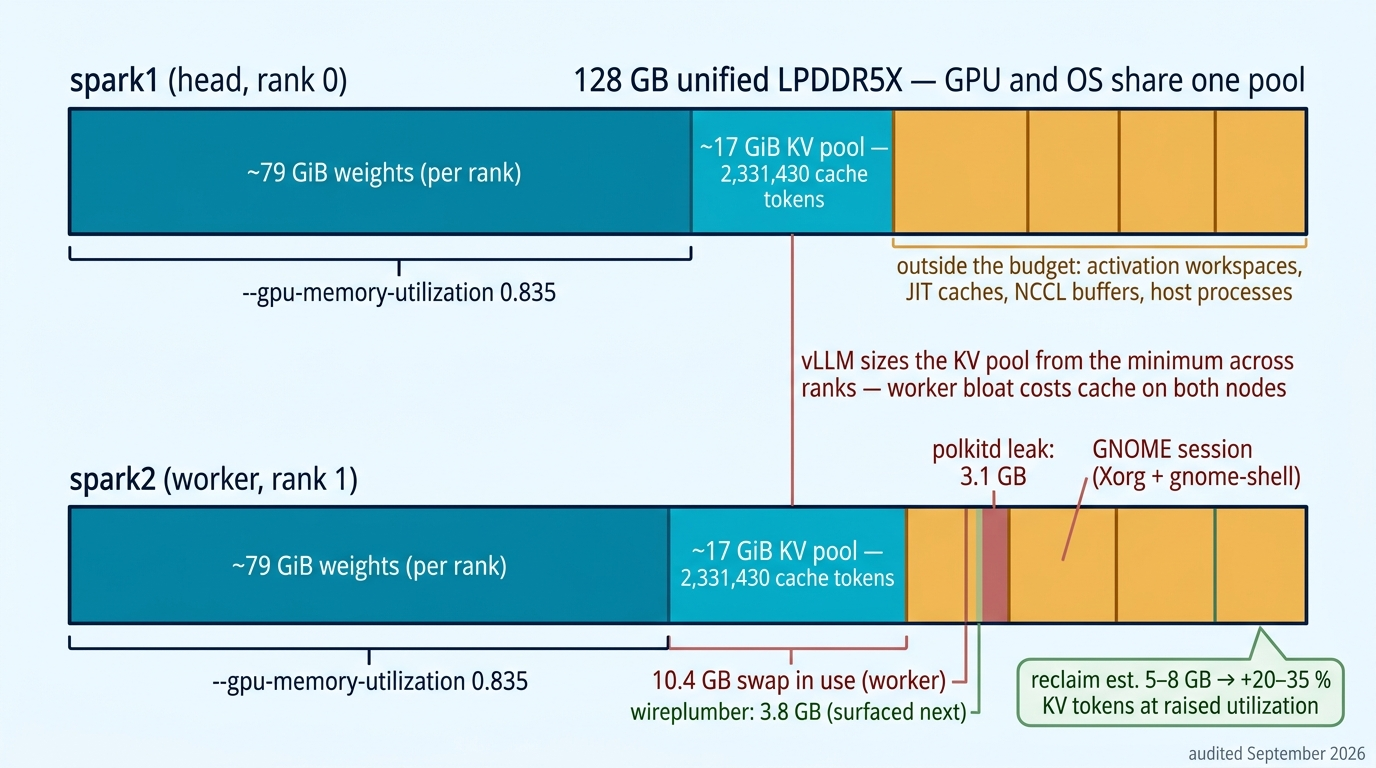
\includegraphics[width=\textwidth]{figures/ch01-128gb-pool.png}
\caption{Unified memory as a contested budget. The utilization target
governs only weights plus KV pool; activation workspaces, JIT caches, NCCL
buffers and every host process spend the same 128\,GB from outside it.
Because vLLM sizes the pool from the \emph{minimum} across ranks, the
worker's 3.1\,GB \code{polkitd} leak and desktop session were shrinking the
KV cache on both nodes (September 2026 audit).}
\label{fig:problem:pool}
\end{figure}

\begin{hbwarning}
The stock \code{earlyoom} daemon on DGX Spark hosts \emph{can} kill vLLM under
deep-context load --- the repository's quick start instructs disabling it on
both hosts. On unified memory, an out-of-memory killer
tuned for desktops is pointed straight at your inference engine.
\end{hbwarning}

\subsection{Bandwidth: decode is a streaming problem}
\label{sec:problem:bandwidth}

Sharing the pool is only half of the platform's tax; the other half is how
slowly the pool moves. LPDDR5X moves roughly 230--250\,GB/s in practice --- an order of magnitude
below datacenter HBM. The 16.5--17\,GB each rank must stream per decode
step is dominated by the touched subset of 256 routed experts across 43
layers, plus attention weights, the drafter, and the language-model head
(\Cref{ch:perf} derives the budget line by line). The arithmetic from the
opening page turns those bytes into $\sim$68\,ms of mandatory reading: a
single stream simply cannot exceed a few dozen steps per second, no matter
how clever the kernels are. Everything that makes this system fast follows
from that arithmetic:

\begin{itemize}
  \item \textbf{speculative decoding} (DSpark, \Cref{ch:specdecode}) makes
    each expensive step emit $\sim$3--4 accepted tokens instead of one;
  \item \textbf{concurrency} amortizes the same weight stream across six
    requests, which is why c=6 aggregate throughput is $\sim$2.2$\times$ a
    single stream;
  \item \textbf{quantization} (FP8 weights, MXFP4 experts, FP8-enveloped KV)
    shrinks the bytes that must move.
\end{itemize}

One lever conspicuously fails: a third machine \emph{does not} speed up a
single stream. The TP=3 experiment cut bytes per rank by a third yet
decoded no faster, because fixed per-step costs --- about 108 NCCL
collectives per decode step --- filled the gap. More hardware is not a
lever here, and \Cref{ch:scaling} proves it the hard way.
\Cref{fig:problem:bytes} puts the bytes, the reading floor, and the three
levers on one page.

\begin{figure}[htbp]
\centering
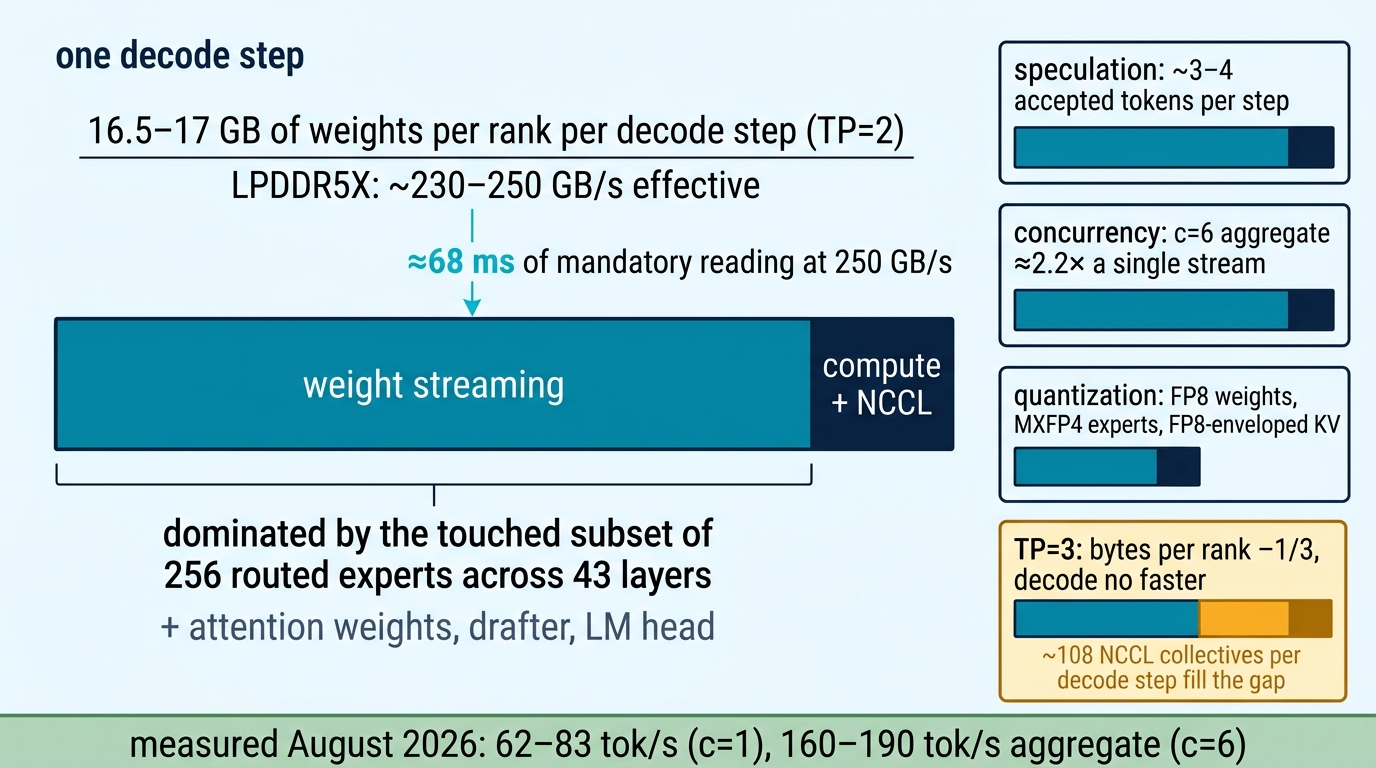
\includegraphics[width=\textwidth]{figures/ch01-decode-step-bytes.png}
\caption{Decode as a streaming problem. Each step must read
16.5--17\,GB of weights per rank through 230--250\,GB/s of LPDDR5X ---
68--74\,ms of mandatory reading before any compute or collective. Only
levers that change the bytes (quantization) or the accepted tokens per step
(speculation, concurrency) move the result; a third machine shrinks the
bytes but refunds the saving in fixed per-step collectives.}
\label{fig:problem:bytes}
\end{figure}

\begin{hblesson}
Before tuning anything, write down the bytes your decode step must stream
and divide by your measured memory bandwidth. If the answer is close to your
observed step time, you are streaming-bound: only fewer bytes per accepted
token (quantization, better draft acceptance) or more tokens per step
(concurrency, speculation) can help. Kernel micro-optimizations cannot.
\end{hblesson}

\section{Two machines, one engine}
\label{sec:problem:twonodes}

The byte budget claims its first casualty before a single request arrives.
The FP8 checkpoint is roughly 157\,GB --- it does not fit in one 128\,GB
node alongside a useful KV cache. The model is therefore sharded with tensor
parallelism across the pair: every layer's weights are split between the two
GPUs, and every decode step synchronizes them over the RoCE link. At TP=2
each rank holds $\sim$79\,GiB of weights, leaving about \textbf{17\,GiB of
KV pool} per rank at the default utilization --- 2{,}331{,}430 cache tokens,
which is what makes the 1M ceiling with multi-session concurrency workable.
Tensor parallelism is doing capacity work here rather than speed work: the
second machine buys the memory to hold the checkpoint, and every decode step
pays for that purchase in synchronization.

\Cref{fig:problem:topology} shows the physical arrangement. One node is the
\emph{head}: it runs rank~0, serves the HTTP API, and orchestrates
everything. The other is the \emph{worker}: rank~1, headless, reached by the
head over SSH for lifecycle operations and over the ConnectX fabric for
NCCL collectives, TCP bootstrap, the scheduler's ZeroMQ broadcasts, and
(optionally) NFS-shared model weights.

\begin{figure}[htbp]
\centering
\begin{tikzpicture}[node distance=6mm and 10mm]
  % Head node
  \node[hbhost, minimum width=52mm, minimum height=42mm] (head) {};
  \node[hbtitle, anchor=north] at ($(head.north)+(0,-1.5mm)$) {spark1 (head, rank 0)};
  \node[hbnode, below=7mm of head.north, minimum width=40mm] (hcpu) {Grace CPU\\\scriptsize launcher, Docker, API};
  \node[hbgpu, below=3mm of hcpu, minimum width=40mm] (hgpu) {Blackwell GPU\\\scriptsize 79 GiB weights + 17 GiB KV};
  \node[hbfaint, below=3mm of hgpu, minimum width=40mm, minimum height=7mm] (hmem) {\scriptsize 128 GB unified LPDDR5X};
  % Worker node
  \node[hbhost, minimum width=52mm, minimum height=42mm, right=34mm of head] (wrk) {};
  \node[hbtitle, anchor=north] at ($(wrk.north)+(0,-1.5mm)$) {spark2 (worker, rank 1)};
  \node[hbnode, below=7mm of wrk.north, minimum width=40mm] (wcpu) {Grace CPU\\\scriptsize headless container};
  \node[hbgpu, below=3mm of wcpu, minimum width=40mm] (wgpu) {Blackwell GPU\\\scriptsize 79 GiB weights + 15--17 GiB KV};
  \node[hbfaint, below=3mm of wgpu, minimum width=40mm, minimum height=7mm] (wmem) {\scriptsize 128 GB unified LPDDR5X};
  % NICs
  \node[hbbox, below=4mm of head, minimum width=40mm] (hnic) {ConnectX-7\\\scriptsize 2 PFs, Gen5 x4 each};
  \node[hbbox, below=4mm of wrk, minimum width=40mm] (wnic) {ConnectX-7\\\scriptsize 2 PFs, Gen5 x4 each};
  \draw[hbflow, very thick] (hnic) -- node[hblabel, above]{200 Gb QSFP (RoCE v2)}
    node[hblabel, below]{NCCL / bootstrap / ZMQ / NFS} (wnic);
  % LAN
  \node[hbfaint, below=9mm of $(hnic.south)!0.5!(wnic.south)$, minimum width=60mm, minimum height=6mm] (lan) {\scriptsize LAN (RJ45): SSH control plane, clients};
  \draw[hbarrow, dashed] (hnic.south) to[out=-90,in=90] (lan.north west);
  \draw[hbarrow, dashed] (wnic.south) to[out=-90,in=90] (lan.north east);
  % Client
  \node[hbnode, left=9mm of head, minimum width=16mm] (client) {clients\\\scriptsize :8888};
  \draw[hbarrow] (client) -- (head.west);
\end{tikzpicture}
\caption{The two-node serving cluster. The model is sharded TP=2 across the
GPUs; every decode step synchronizes over the direct 200\,Gb RoCE link, while
lifecycle control (SSH) and client traffic ride the ordinary LAN.}
\label{fig:problem:topology}
\end{figure}

Splitting one engine across two commodity hosts buys the memory the model
needs, but it also buys a distributed-systems tax that recurs throughout
this book: the pair fails \emph{as a pair}. A rank stalled in a mid-serve
JIT compilation leaves its peer blocked in a collective until the torch NCCL
watchdog kills it after 600 seconds (\ghissue{117}). A reboot can resurrect
one rank but not the other. A patch applied to one writable container layer
but not the other produces divergent engines. Much of the operational
discipline in \Cref{ch:patches,ch:operations} exists precisely to keep two
loosely coupled machines behaving like one engine.

\section{The economics, briefly}
\label{sec:problem:econ}

After a chapter spent pricing constraints --- shared memory,
streaming-bound decode, a pair that fails as a pair --- it is worth naming
what they buy: why this configuration is interesting beyond its own
walls. Two DGX Sparks cost on the order of a used car, sit under a desk, and
draw the modest power that opened this chapter. For that, the operators get a private frontier-class model with a million
tokens of context, native vision, tool calling, and $\sim$190\,\tokspersec{}
aggregate throughput --- enough to run a small team's agents with no per-token
bill and no data leaving the room. The price is paid in engineering instead:
the roughly forty runtime patches, the measurement rigs, and the operational
doctrine that the rest of this handbook documents. Whether that trade is
right for any given team is situational; what this system demonstrates is
that the trade is \emph{available}, and what it actually costs.

\FloatBarrier
The 26 watts on the opening page are no longer a puzzle. A decode step on
this cluster is not a computation with a memory cost; it is a memory read
--- 16.5--17\,GB per rank through 230--250\,GB/s, 68--74\,ms of it ---
with a computation attached, and the second machine is there to hold the
checkpoint rather than to go faster. The 128\,GB is not a GPU budget either:
it is a budget two operating systems are already spending from, which makes
the KV pool a residual rather than an allocation.

\section*{Takeaways}
\begin{itemize}
  \item The mission: DeepSeek-V4-Flash (MoE + MLA + sparse indexer + DSpark
    drafter + vision) at a 1M-token ceiling and six concurrent agent
    sessions, on two GB10 DGX Sparks with vLLM at TP=2 --- where the second
    machine buys the memory for a $\sim$157\,GB checkpoint, not speed, and
    every decode step pays for that purchase in synchronization.
  \item Unified memory makes host RAM part of the GPU budget: OS daemons,
    JIT caches, activation workspaces and NCCL buffers spend the same
    128\,GB from \emph{outside} the utilization target, an OOM killer tuned
    for desktops targets the engine, and because vLLM sizes the pool from
    the minimum across ranks, one node's leak shrinks the cache on both.
    Capacity work therefore starts with host hygiene --- the audit put the
    reclaimable 5--8\,GB at +20--35\,\% KV tokens at a raised utilization.
  \item Decode is weight-streaming-bound: only fewer bytes per accepted
    token (quantization, better acceptance) or more tokens per step
    (speculation, concurrency) move it at c=1. A third machine does not:
    TP=3 cut bytes per rank by a third and decoded no faster, because the
    $\sim$108 fixed collectives per step refunded the saving.
  \item A TP pair fails as a pair: a rank stalled in mid-serve JIT leaves
    its peer blocked until the 600-second NCCL watchdog fires
    (\ghissue{117}), reboots can resurrect one rank and not the other, and
    a patch applied to one container layer produces divergent engines ---
    the pair-level hazards that shape the operational doctrine of later
    chapters.
\end{itemize}

\chaptertransition{Constraints this tight leave no room for an engine you
cannot account for. If the KV pool is whatever two operating systems have
not already spent, and if the two machines fail as a unit, then ``which
bytes are actually running, on both ranks?'' stops being a hygiene question
and becomes a capacity and reliability question --- one that has to be
answered by construction rather than by inspection after the fact. The next
chapter opens a stack whose answer is deliberately strange: about forty
source patches applied to the inference engine at every container start,
each chained with \code{|| exit 1}, on top of a prebuilt image the
repository refuses to rebuild. A serving stack built to fail its own boot
--- why would anyone run a frontier model that way?}

\chapter{Architecture Overview}
\label{ch:architecture}

This serving stack is built to fail its own boot. About forty source
patches are applied to the inference engine at container start, each one
validated against pinned bytes and chained with \code{|| exit 1}. If a
single patch no longer applies cleanly, the container dies before
\code{exec vllm} ever runs --- a failed patch is a failed boot, never a
silently stock server. The engine itself is a prebuilt image that the
repository never rebuilds, pinned by manifest digest; the checkpoint is
pinned by revision. Why would anyone run a heavily modified engine this way
instead of maintaining a fork?

That question is the key to the whole design. Most serving stacks are
described by what they contain; this one is better described by what it
\emph{refuses to do}. It refuses to fork and rebuild its inference engine,
refuses to run unpinned artifacts, and refuses to boot if any of its
runtime modifications cannot be proven to apply cleanly. The result is a
layered architecture in which every layer is either pinned by cryptographic
digest or applied fail-closed at boot. This chapter walks the layers top to
bottom, follows one request through the running system, and introduces the
community lineage that produced it --- the map the remaining chapters fill
in.

For an inference engineer, the practical stakes are provenance and
rollback: when a two-node engine misbehaves, the first question is always
\emph{which bytes are actually running}. This architecture is arranged so
that the question has a checkable answer. Understanding what is pinned,
what is patched, and what fails closed is prerequisite to every debugging,
patching, and operations chapter that follows --- and it is the reason
fixes made here are portable to anyone else running the same pinned image.

\section{The layer cake}
\label{sec:architecture:layers}

\Cref{fig:architecture:stack} shows the stack. Rather than walking it as an
inventory, read it through the three refusals --- every layer exists to
enforce one of them.

\paragraph{What is pinned.} Two layers answer ``which bytes are running.''
The checkpoint, \code{deepseek-ai/DeepSeek-V4-Flash-Vision-Exp}, is pinned
to revision \code{86f746b3}\ldots{} in the HuggingFace cache, and it
supplies not only weights but executable behavior. Its
\repofile{encoding/encoding_dsv4.py} package replaces the usual Jinja chat
template: message rendering, reasoning-effort control, and DSML tool-call
parsing are all checkpoint Python that the runtime installs into vLLM at
boot (\Cref{ch:model}). Above it sits the runtime image, the prebuilt
Anemll \repofile{ghcr.io/anemll/dspark-vllm-gx10:0.1.1}, pinned by
manifest digest (\code{sha256:a8394849}\ldots) in
\repofile{.env.dspark.example} --- a vLLM fork
(\code{0.25.2.dev0+g752a3a504}) with GB10 kernels: the B12X MoE backend,
FlashInfer's SM120 sparse-MLA family, DeepGEMM, Triton, and TileLang. The
repository never rebuilds this image; it \emph{patches} it.

\paragraph{What is patched.} The patch train: about forty source patches,
mounted read-only into the container and applied by the Compose entrypoint
\emph{before} \code{exec vllm} --- the fail-closed mechanism from the
opening page, formalized and enforced in \Cref{ch:patches}. The
orchestration around the train is what keeps two machines applying it
identically. The Compose entrypoint \emph{is} the patch orchestrator; the
launcher, \repofile{start-deepseek-v4-flash-dspark.sh}, normalizes
configuration, validates the fabric, syncs patches to the worker over SSH,
runs patcher preflights on both ranks, starts worker-first, then
health-polls, smokes, and warms the JIT caches (\Cref{ch:operations}).

\paragraph{What is proven.} Configuration is one file,
\repofile{.env.dspark}, sourced through a normalizing snapshot (BOM/CRLF
stripped, atomically published to the worker with mode 0600). Every switch
is documented in a three-lane matrix --- registered on this image,
Stage-C-only no-op, or launcher-side --- in \repofile{docs/ENVS.md}
(\Cref{ch:profile}). The whole assembly is then verified twice. A CPU-only
CI gate (\repofile{scripts/ci-validate.sh}) locks wiring, defaults, and
fail-closed behavior on every push, while a live audit suite ---
throughput, speculative-decode health, long-context retrieval, tool
batteries, garble sweeps --- answers ``is this deployment actually good?''
on the real pair (\Cref{ch:measurement}).

Taken together the three refusals produce one property worth naming: at any
moment the running system reduces to a short checkable list --- a checkpoint
revision, an image digest, a set of per-patch byte hashes, and one normalized
configuration snapshot.

\begin{figure}[htbp]
\centering
\begin{tikzpicture}[node distance=3.2mm]
  \node[hbbox, text width=118mm] (verify) {\textbf{Verification} --- CPU CI gates (wiring, defaults) + live audit suite (tok/s, RULER, tools, garble)};
  \node[hbbox, text width=118mm, below=of verify] (ops) {\textbf{Orchestration} --- launcher (fabric validation, worker sync, preflights, worker-first boot, warmup) + ops scripts};
  \node[hbnode, text width=118mm, below=of ops] (cfg) {\textbf{Configuration} --- \detokenize{.env.dspark} snapshot $\rightarrow$ Compose interpolation $\rightarrow$ container env};
  \node[hbpatch, text width=118mm, below=of cfg] (patch) {\textbf{Patch train} --- $\sim$40 fail-closed, source-locked boot-time patches (\detokenize{|| exit 1})};
  \node[hbgpu, text width=118mm, below=of patch] (image) {\textbf{Runtime image} --- Anemll dspark-vllm-gx10:0.1.1, digest-pinned (vLLM fork + GB10 kernels)};
  \node[hbnode, text width=118mm, below=of image] (ckpt) {\textbf{Checkpoint} --- DeepSeek-V4-Flash-Vision-Exp @ pinned revision (weights + encoding\_dsv4.py)};
  \node[hbhost, text width=118mm, below=of ckpt] (hw) {\textbf{Hardware} --- 2$\times$ DGX Spark (GB10, 128 GB unified) + 200 Gb RoCE};
  \draw[hbarrow] (verify.south) -- (ops.north);
  \draw[hbarrow] (ops.south) -- (cfg.north);
  \draw[hbarrow] (cfg.south) -- (patch.north);
  \draw[hbarrow] (patch.south) -- (image.north);
  \draw[hbarrow] (image.south) -- (ckpt.north);
  \draw[hbarrow] (ckpt.south) -- (hw.north);
\end{tikzpicture}
\caption{The layer cake. Every layer is pinned (digest, revision, byte hash)
or applied fail-closed at boot; nothing is rebuilt, and nothing unproven is
allowed to serve. None of this is small machinery: the Compose file runs
463 lines and the launcher 1{,}753.}
\label{fig:architecture:stack}
\end{figure}

\begin{hblesson}
The central architectural bet: \emph{pin a prebuilt image and patch it at
boot} rather than maintaining a fork.
\end{hblesson}

That bet is the answer to the opening question. The pin gives byte-exact
provenance and trivially reproducible bug reports. Boot-time patching keeps
every local change a small, reviewable, individually revertable diff, and
container recreation is a guaranteed rollback to pristine upstream bytes
--- together, three properties a privately maintained fork surrenders.
\Cref{ch:patches} examines what this discipline costs and how it is
enforced, and \Cref{fig:architecture:bet} sets the two options side by side.

\begin{figure}[htbp]
\centering
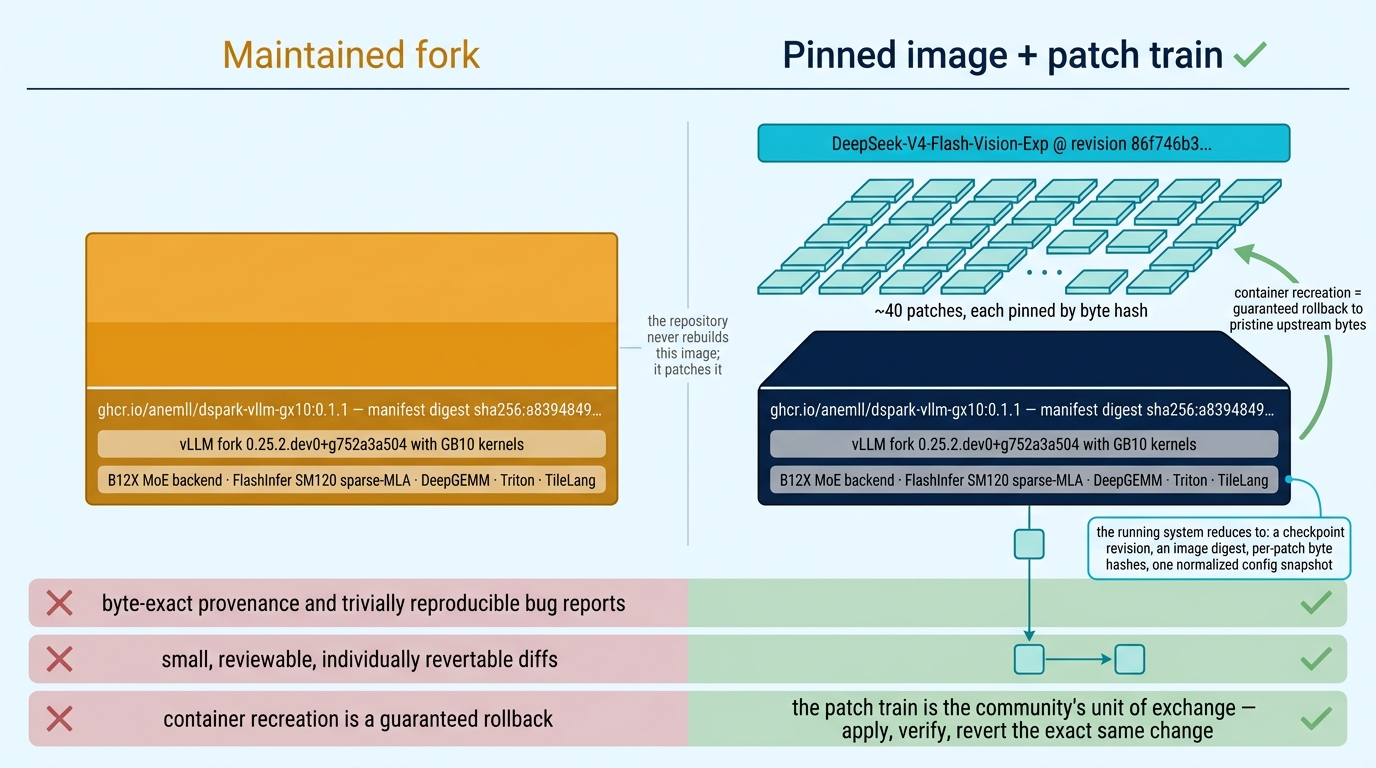
\includegraphics[width=\textwidth]{figures/ch02-central-bet.png}
\caption{The architectural bet. A maintained fork fuses local changes into
rebuilt bytes; pinning a prebuilt image and applying the patch train at boot
keeps every modification a separable, hash-pinned diff on top of bytes anyone
else can obtain. The three properties on the right are exactly what a private
fork surrenders --- and they are what makes a fix here portable to another
operator of the same image.}
\label{fig:architecture:bet}
\end{figure}

\section{The life of a request}
\label{sec:architecture:request}

The path below repays two readings: one for the sequence, one for how many
of its steps are behavior this repository added rather than inherited. To
see the layers in motion, follow one chat completion through the running
system (\Cref{fig:architecture:request}):

\begin{enumerate}
  \item A client POSTs an OpenAI-style request to
    \code{http://head:8888/v1/chat/completions} --- messages, optional
    images, tools, sampling parameters, and per-request
    \code{chat_template_kwargs} controlling thinking effort.
  \item vLLM's API layer validates it. Several of this system's patches
    live here: image parts are rejected outside \code{user} turns, truncated
    tool calls will later be re-labeled, and (opt-in) named-tool responses
    are contract-checked before returning.
  \item The \emph{checkpoint's own encoder} --- installed at boot as
    \repofile{vllm/tokenizers/deepseek_v4_encoding.py} --- renders messages
    into token IDs: role headers, \code{<think>} markers, DSML tool-result
    encoding, image placeholder tokens.
  \item The scheduler admits the request into continuous batching. Long
    prompts are \emph{chunk-prefilled} 1{,}024 tokens at a time, with an
    admission cap on concurrent partial prefills so decoding requests are
    never starved --- the hardest-won scheduler behavior in the repository
    (\ghissue{27}, \ghissue{43}; \Cref{ch:bugs}).
  \item Each engine step runs on both ranks: the head broadcasts the step
    plan to the worker over ZeroMQ; each rank streams its weight shard,
    computes, and synchronizes through $\sim$108 NCCL collectives per decode
    step over the RoCE link.
  \item The DSpark drafter proposes a block of six tokens; the target model
    verifies them in one pass; accepted tokens (typically 3--4) are appended.
    Prefix caching stores computed KV so a follow-up turn reuses the
    conversation's prefix (\Cref{ch:specdecode}).
  \item The detokenizer streams text out --- with client \code{stop} strings
    held dormant inside \code{<think>} (a patch) --- and the reasoning and
    tool-call parsers split the stream into \code{reasoning}, \code{content},
    and structured \code{tool_calls} for the response.
\end{enumerate}

\begin{figure}[htbp]
\centering
\adjustbox{max width=\textwidth}{%
\begin{tikzpicture}[node distance=4mm and 7mm]
  \node[hbnode] (cli) {client};
  \node[hbbox, right=of cli] (api) {API layer\\\scriptsize validation,\\\scriptsize contracts};
  \node[hbbox, right=of api] (enc) {encoder\\\scriptsize encoding\_dsv4\\\scriptsize $\rightarrow$ token IDs};
  \node[hbbox, right=of enc] (sched) {scheduler\\\scriptsize chunked prefill,\\\scriptsize admission caps};
  \node[hbgpu, right=of sched] (eng) {TP=2 engine\\\scriptsize rank 0 + rank 1\\\scriptsize NCCL over RoCE};
  \node[hbbox, below=of eng] (spec) {DSpark\\\scriptsize draft 6, verify 1 pass};
  \node[hbbox, left=of spec] (detok) {detokenizer\\\scriptsize stop guard};
  \node[hbbox, left=of detok] (parse) {parsers\\\scriptsize reasoning / tools};
  \node[hbnode, left=of parse] (resp) {response\\\scriptsize SSE stream};
  \draw[hbflow] (cli) -- (api);
  \draw[hbflow] (api) -- (enc);
  \draw[hbflow] (enc) -- (sched);
  \draw[hbflow] (sched) -- (eng);
  \draw[hbflow] (eng) -- (spec);
  \draw[hbflow] (spec) -- (detok);
  \draw[hbflow] (detok) -- (parse);
  \draw[hbflow] (parse) -- (resp);
  \draw[hbarrow, dashed] (spec.east) to[out=0,in=-20] node[hblabel, right]{accepted tokens} (eng.east);
\end{tikzpicture}%
}
\caption{The life of a request. Patched behavior (validation contracts, the
checkpoint encoder, admission caps, the stop-string guard) sits at almost
every stage.}
\label{fig:architecture:request}
\end{figure}

\section{Head and worker: one engine, two roles}
\label{sec:architecture:roles}

The request walkthrough treated the two ranks as interchangeable halves of
one engine; keeping them that way is a design goal in its own right. The
two containers run the \emph{same} image, the same entrypoint, and the
same patch train --- divergence between ranks is itself a failure mode the
launcher works to prevent. They differ only in role variables:
\envvar{NODE_RANK=0} on the head, which binds the HTTP server; and
\envvar{NODE_RANK=1} with \envvar{HEADLESS=1} on the worker, whose
healthcheck short-circuits to success because there is no port to probe.
The launcher enforces \emph{worker-first} startup: rank~1 must be waiting
before rank~0 initializes its TCPStore. The converse holds too --- stopping
is always pairwise, because a surviving lone rank is stale, not healthy
(\Cref{ch:operations}). \Cref{fig:architecture:boot} walks the ordering and
the hazard beside it.

\begin{hbwarning}
Docker's \code{restart: unless-stopped} policy can resurrect the two ranks
\emph{independently} after host reboots --- a split-brain hazard where one
rank is fresh and the other stale. The launcher detects an already-running
head and exits with code 3 (``already up, not an error''), and the
documentation is explicit that exit 3 is \emph{not} a health claim.
Supervised deployments set \envvar{DSPARK_RESTART_POLICY=no} and let the
unit own the lifecycle.
\end{hbwarning}

\begin{figure}[htbp]
\centering
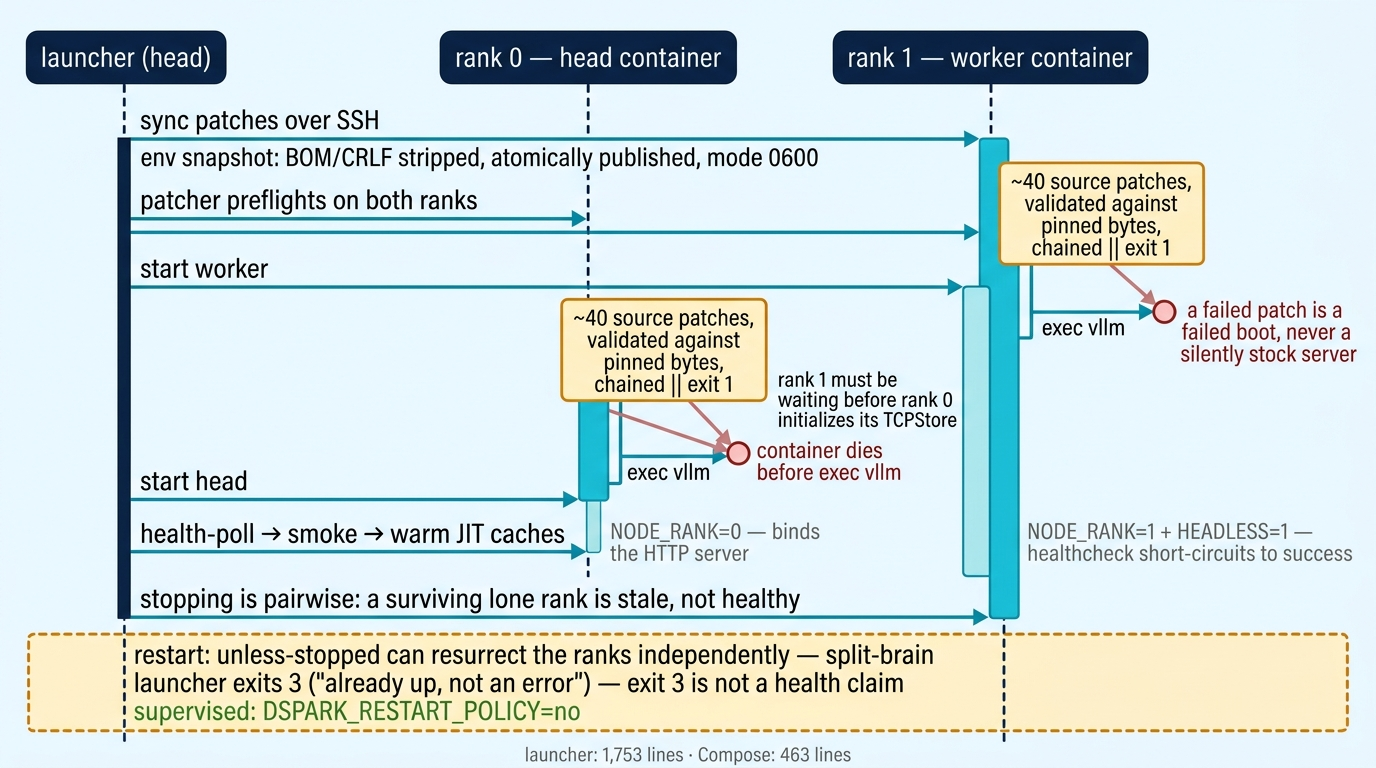
\includegraphics[width=\textwidth]{figures/ch02-boot-gate.png}
\caption{Boot, in order. The launcher normalizes configuration, validates the
fabric, syncs patches over SSH and preflights both ranks, then starts the
worker first so rank~1 is waiting before rank~0 initializes its TCPStore.
Inside each container the patch train runs before \code{exec vllm} and any
failure kills the container rather than serving stock bytes; the hazard lane
shows the converse, an unsupervised restart policy resurrecting the two ranks
independently.}
\label{fig:architecture:boot}
\end{figure}

\section{Provenance and lineage}
\label{sec:architecture:lineage}

Fail-closed patching earns its keep at boot; the pinning half of the bet
pays off somewhere less obvious. Because the runtime is a \emph{pinned
communal image} rather than a private fork, every fix in \Cref{ch:bugs} exists as a portable patch against known
bytes --- other operators of the same image can apply, verify, and revert
the exact same change. The patch train is not just a deployment mechanism;
it is the community's unit of exchange. And the community is real: this
system is the fourth generation of a lineage recorded in
\repofile{docs/SETUP.md} and \repofile{CREDITS.md}. The chain that follows
is operational information rather than courtesy: each generation owns a
distinct layer of what runs today, so placing a behavior in the lineage
narrows where its patches and its documentation live.

The chain runs from \textbf{Rafael Caricio}, who built the original
DSpark--vLLM integration and the control replica (single-stream,
unpatched), through \textbf{tonyd2wild}, who packaged the reproducible
two-node recipe --- self-contained Compose, a direct \code{vllm serve} launch,
and the worker-first start script from Mia's AI Lab --- that this repository descends
from. \textbf{drowzeys (``Keys'')} wrote the
concurrency patches that made batched DSpark \emph{correct} ---
request-stable KV slots and the ragged context path (\Cref{ch:specdecode})
--- plus the abliterated checkpoint variants.

\textbf{Anemll} ships the prebuilt GB10 image that became the pinned
runtime, replacing an earlier locally built ``Stage-C'' overlay stack that
survives as an optional lane (\Cref{ch:scaling}).
\textbf{localaiguyy} contributed the attention-group padding that unlocks a
third node (TP=3). \textbf{Mia's AI Lab} operates the cluster and maintains
the repository --- including the issue tracker whose numbered incidents
(\ghissue{21} through \ghissue{211}) structure \Cref{ch:bugs}.

\section{A map of this book}
\label{sec:architecture:map}

The remaining chapters follow the layers. \Cref{ch:model} descends into the
model itself; \Cref{ch:profile} reads the serving configuration flag by
flag; \Cref{ch:fabric} covers the network layer beneath TP.
\Cref{ch:patches} formalizes the patch discipline and \Cref{ch:bugs}
chronicles the bugs it exists to fix. \Cref{ch:specdecode} treats
speculative decoding in production depth, \Cref{ch:perf} builds the
performance model and recounts the tuning campaigns, and
\Cref{ch:measurement} documents the benchmarking doctrine that keeps the
numbers honest. \Cref{ch:operations} is the runbook; \Cref{ch:scaling}
surveys the paths beyond two nodes; \Cref{ch:lessons} distills what
transfers to any inference deployment.

\FloatBarrier
The stack is no longer software that was installed; it is a short list of
pins plus a diff applied at boot. Ask which bytes are serving and the answer
is enumerable --- one checkpoint revision, one image digest, a set of
per-patch byte hashes, one normalized configuration snapshot --- and
anything that cannot be proven against that list kills the container instead
of quietly serving stock behavior. The patch train from the opening page is
not debt owed to a fork nobody wrote; its diffs are the unit in which this
system is modified, exchanged with other operators, and rolled back.

\section*{Takeaways}

\begin{itemize}
  \item The architecture is defined by pins: checkpoint revision, image
    manifest digest, and per-patch byte hashes --- plus fail-closed
    boot-time patching instead of a forked rebuild.
  \item That bet buys three properties a private fork surrenders:
    byte-exact provenance and reproducible bug reports, local changes that
    stay small and individually revertable, and rollback by container
    recreation to pristine upstream bytes --- which is also what makes a
    fix here portable to anyone running the same pinned image.
  \item A request crosses patched behavior at nearly every stage: API
    contracts, the checkpoint's own encoder, scheduler admission caps, the
    draft/verify loop, and the stop-string-aware detokenizer.
  \item Divergence is failure: head and worker run identical bytes with
    different role variables, boot worker-first, and stop pairwise ---
    and exit 3 (``already up'') is explicitly not a health claim.
\end{itemize}

\chaptertransition{Pins and patches settle \emph{which} bytes are running;
they say nothing about what those bytes do once a request arrives. Much of
the patch train exists because some property of this particular checkpoint
--- a KV cache that tensor parallelism cannot shard, an FFN that routes on
raw token ids, a drafter whose state lives outside the engine's cache ---
made stock behavior wrong, so the train cannot be read, extended,
or safely reverted by anyone who does not know the model's anatomy. The next
chapter opens it, beginning with a configured KV dtype whose name is the
only thing separating it from another: identical bytes, different dispatch,
and one string comparison that quietly cost long-context decode a factor of
sixteen.}

% =============================================================================
% Chapter 3 — The Model: DeepSeek-V4-Flash Through a Serving Lens
% =============================================================================
\chapter{The Model: DeepSeek-V4-Flash Through a Serving Lens}
\label{ch:model}

A single string comparison once cost this stack a factor of
$\approx$16$\times$ on decode past 600K tokens. The configured KV dtype,
\code{nvfp4_ds_mla}, stores bytes identical to \code{fp8_ds_mla} --- the
name changes only kernel dispatch. But a dispatch check tested the string
rather than the layout, and \code{nvfp4_ds_mla} fell into the slow bf16-KV
decode path until a one-line fix widened the comparison (issue
\ghissue{22}). No amount of staring at the serving configuration diagnoses
that class of failure; it takes knowing what the model actually holds in
memory and moves every step.

That is the knowledge this chapter supplies. DeepSeek-V4-Flash is not a
generic dense transformer: it is a 43-layer MoE model with latent-KV attention
that every tensor-parallel rank replicates in full, a sparse-attention indexer
that selects which 512 compressed rows each query may read, a speculative
drafter grafted onto the target's own hidden states, and a checkpoint-supplied
Python encoder in place of a chat template. Each of those choices creates a
serving consequence --- a KV byte layout, a collective pattern, a failure mode
--- that later chapters measure, patch, and occasionally get burned by. This
chapter teaches the mechanism, assuming you have never opened the model's
\repofile{config.json}.

For an inference engineer, this chapter converts the model from a black box
into a set of budgets and invariants: why KV capacity quotes are per rank
and replicated, why the FFN forward needs raw token ids, why the drafter
keeps its state outside the vLLM KV cache, why the legal values of $k$
depend on the checkpoint lineage. The bugs, patches, and performance
ceilings in the rest of the book are downstream of these mechanisms, and
most are difficult even to describe without the vocabulary established
here.

\section{The shape of the network}
\label{sec:model-shape}

The checkpoint loads as \code{DeepseekV4ForCausalLM}. The load-bearing facts
from \repofile{config.json} and the model source
(\repofile{recipe/overlay/vllm/models/deepseek_v4/nvidia/model.py}) are
summarized in \Cref{tab:model-config} and drawn as a data-flow diagram in
\Cref{fig:model-block}.

\begin{table}[htbp]
  \centering\small
  \caption{DeepSeek-V4-Flash architecture facts that matter for serving.}
  \label{tab:model-config}
  \begin{tabular}{@{}l>{\raggedright\arraybackslash}p{5.4cm}>{\raggedright\arraybackslash}p{5.0cm}@{}}
    \toprule
    Property & Value & Serving consequence \\
    \midrule
    Decoder layers & 43 (+ MTP draft layers after) & 43 MoE gates per forward \\
    Hidden size & 4096 & mHC streams collapse to this \\
    Attention & MLA, 64 heads $\times$ head\_dim 512 & latent KV, replicated per rank \\
    RoPE dims & 64 (rest is NoPE) & bf16 RoPE slice in every KV row \\
    Routed experts & 256, top-6, + 1 shared & expert streaming dominates decode \\
    MoE layers 0--2 & hash-routed (\code{tid2eid}) & FFN needs raw \code{input_ids} \\
    Expert weights & \code{fp4_e8m0_k32} (MXFP4/E8M0) & no NVFP4 tensor-core path today \\
    Other linears & FP8, $128\times128$ blocks & fp8 output pipeline end-to-end \\
    Indexer & 64 heads $\times$ 128 dims, top-512 & replicated across TP ranks \\
    Sliding window & 128 tokens & 3 SWA KV groups beside MLA \\
    Context & 1{,}048{,}576 (YaRN $\times$16 from 64K) & KV capacity is the ceiling \\
    \code{dspark_block_size} & 5 & drafter predicts a 5-token block \\
    \code{num_nextn_predict_layers} & 1 (0731) / 3 (Vision-Exp) & draft stage count; $k$ divisibility \\
    \bottomrule
  \end{tabular}
\end{table}

Three structural decisions deserve a mechanism-level explanation before
anything else in the stack is comprehensible.

\subsection{MLA: why every rank holds the whole KV cache}

Multi-head Latent Attention stores, per token, a single low-rank \emph{latent}
vector rather than per-head K and V tensors. The 64 attention heads are
projected out of that shared latent at read time through the fused
\code{wqa|wkv} projection (replicated) and a grouped
\code{wo_a}/\code{wo_b} output path (sharded, 8 output groups). Tensor
parallelism therefore shards the \emph{compute} --- heads, output groups,
expert slices --- but not the cache: there is no per-head axis in the stored
latent to cut. On the two-Spark TP=2 deployment both ranks hold the full KV
pool, byte for byte. The fable5-1 audit (\Cref{ch:perf}) states the
consequence plainly: with TP the whole KV is replicated on both ranks, and
only decode-context parallelism (not wired for the DSV4 sparse backends in the
pinned image) would ever shard it. When that chapter discusses capacity, ``17.04\,GiB of KV''
means 17.04\,GiB \emph{per rank}, twice. If you take one asymmetry from this
chapter, take that one: MLA shards compute and not cache, so every
KV capacity figure in this book is a per-rank figure the cluster pays for
on both ranks. \Cref{fig:tp2-split} draws where the TP=2 cut falls.

\begin{figure}[htbp]
\centering
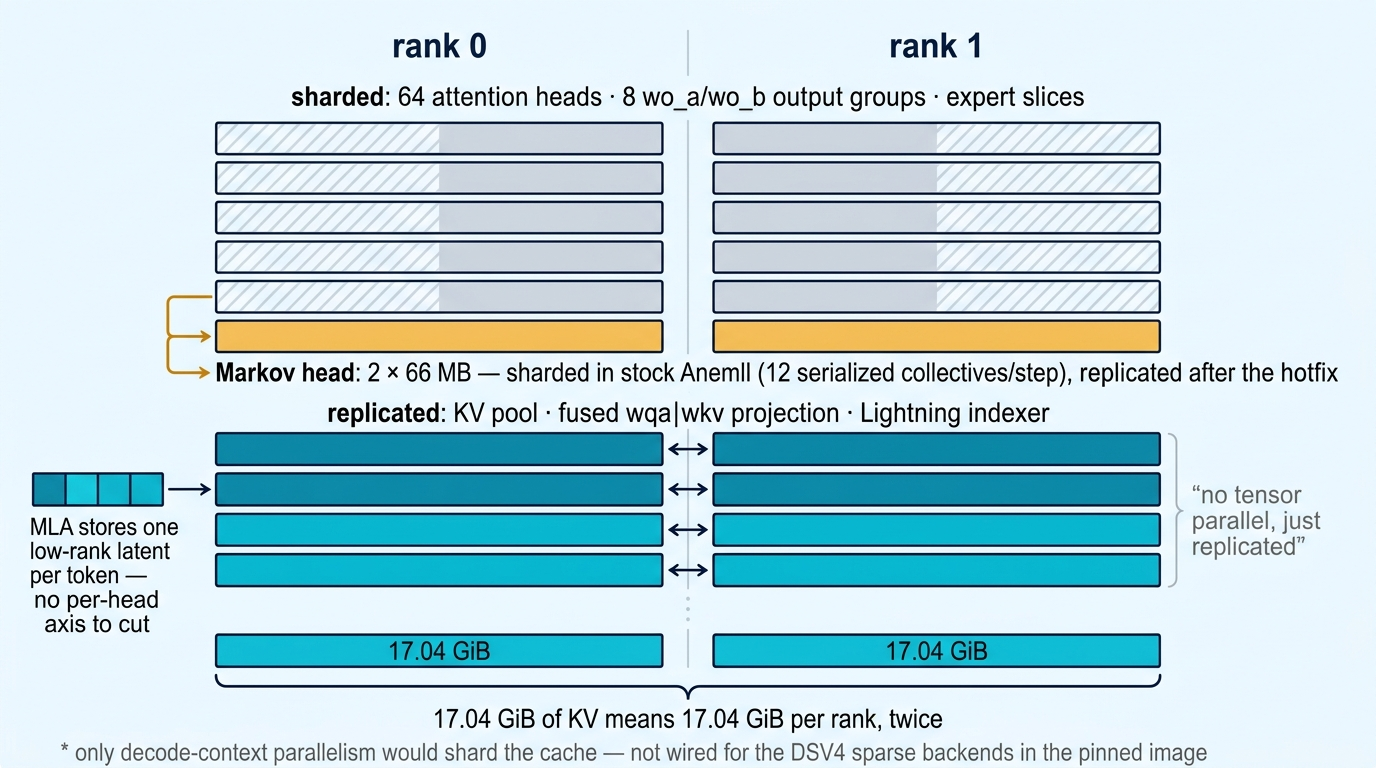
\includegraphics[width=\textwidth]{figures/ch03-tp2-split.png}
\caption{Tensor parallelism shards compute, not cache. Attention heads,
output groups and expert slices are split across the two ranks; the latent
KV pool, the fused projection and the Lightning indexer are held whole on
both, because MLA stores a single low-rank latent per token with no per-head
axis to cut. Every KV capacity figure in this book is therefore a per-rank
figure the cluster pays for twice.}
\label{fig:tp2-split}
\end{figure}

The layers are threaded together by hyper-connection (``mHC'') residual
streams: several parallel residual lanes with a pre/post mixing op around each
attention and FFN block, fused between layers. This detail matters to serving
because the DSpark drafter must capture per-layer features, and collapsing the
mHC streams early breaks the fused chain --- the origin of the deferred-capture
machinery described in \Cref{sec:model-dspark}.

\subsection{Hash-routed MoE on layers 0--2}

Layers 0--2 carry MoE blocks with \emph{no router GEMM}. Expert choice is a
pure table lookup, \code{gate.tid2eid[token_id]}: the token's vocabulary id
selects its experts. This is why the FFN forward signature takes
\code{input_ids} --- a fact that ripples surprisingly far. The multimodal
runner ordinarily drops \code{input_ids} once embeddings exist; Vision-Exp had
to force \code{requires_raw_input_tokens = True} to keep hash routing alive
(\Cref{sec:model-vision}). Every other MoE layer routes with a learned gate
plus a noaux-tc correction bias, top-6 of 256 routed experts, plus one shared
expert that always runs.

\subsection{Quantization: FP8 weights, MXFP4 experts}

The checkpoint metadata says FP8 weights, and the attention/dense linears are
FP8 with $128\times128$ block scales. The 256 routed experts, however, ship in
\code{fp4_e8m0_k32}: MXFP4 values with power-of-two E8M0 scales per 32-element
block. On the GB10 boards the b12x MoE backend consumes this as W4A16
(dequantize to bf16, then MMA) because its NVFP4 tensor-core path accepts only
\code{modelopt_nvfp4}-format weights --- a kernel-level gap
\Cref{ch:perf} quantifies for prefill. Expert scale tensors are loaded with
\code{view(uint8)} rather than numeric casts, because a dtype conversion would
destroy the raw exponent bytes.

\begin{figure}[htbp]
\centering
\begin{tikzpicture}[node distance=5mm and 15mm]
  % --- target stack (left column) ---
  \node[hbbox, minimum width=58mm] (embed)
    {Embedding (vocab 129{,}280)};
  \node[hbnode, minimum width=58mm, below=of embed] (early)
    {\textbf{Layers 0--2}\\[1pt]
     {\scriptsize MLA (layers 0--1 SWA-only)}\\
     {\scriptsize MoE hash-routed: tid2eid[token\_id]}};
  \node[hbnode, text width=56mm, below=of early] (mid)
    {\textbf{Layers 2--42} (alternating)\\[1pt]
     {\scriptsize 21$\times$ C4A: Lightning indexer $\to$ top-512 sparse MLA}\\
     {\scriptsize 20$\times$ C128A: coarse compressed MLA}\\
     {\scriptsize each + MoE: 256 routed top-6 + 1 shared}};
  \node[hbbox, text width=54mm, align=center, below=of mid] (lmhead)
    {hc\_head collapse $\to$ lm\_head\\{\scriptsize (bf16, sharded)}};
  \node[hbnode, minimum width=58mm, below=of lmhead] (verify)
    {sample + verify draft block\\{\scriptsize (rejection sampling)}};
  % --- drafter (right column) ---
  \node[hbfaint, minimum width=44mm, right=of mid] (capture)
    {feature capture at\\dspark\_target\_layer\_ids\\{\scriptsize mHC streams mean-pooled}};
  \node[hbpatch, minimum width=44mm, below=6mm of capture] (draft)
    {\textbf{DSpark draft block}\\[1pt]
     {\scriptsize stacked mtp stages (1 or 3)}\\
     {\scriptsize one non-causal parallel pass}\\
     {\scriptsize over [anchor $|$ noise $\times$ $k$]}};
  \node[hbpatch, minimum width=44mm, below=6mm of draft] (markov)
    {Markov head, rank 256\\{\scriptsize logits += W1[prev]\,W2$^{\top}$, left-to-right}};
  % --- arrows ---
  \draw[hbflow] (embed) -- (early);
  \draw[hbflow] (early) -- (mid);
  \draw[hbflow] (mid) -- (lmhead);
  \draw[hbflow] (lmhead) -- (verify);
  \draw[hbarrow, dashed] (mid.east) -- (capture.west)
    node[hblabel, midway, font=\tiny, align=center, fill=white,
         inner sep=1pt] {stable\\buffers};
  \draw[hbarrow] (capture) -- (draft);
  \draw[hbarrow] (draft) -- (markov);
  \draw[hbok] (markov.south) -- ++(0,-4mm) -|
    node[hblabel, pos=0.25, below] {$k$ draft tokens} (verify.south);
  \draw[hbarrow, dashed] (verify.west) -- ++(-13mm,0) |- (embed.west)
    node[hblabel, pos=0.5, above=1mm, align=center] {accepted\\tokens};
  \begin{scope}[on background layer]
    \node[hbgroup, fit=(capture)(draft)(markov),
      label={[hbtitle]above:DSpark drafter (no vLLM KV)}] {};
  \end{scope}
\end{tikzpicture}
\caption{DeepSeek-V4-Flash as served: the 43-layer target stack (left) with the
DSpark drafter (right) hanging off captured target-layer features. The drafter
predicts a whole block in one non-causal pass and keeps its own sliding-window
state outside the vLLM KV cache.}
\label{fig:model-block}
\end{figure}

\section{The sparse attention stack}
\label{sec:model-sparse}

Full attention over a million tokens is not an option on this hardware, and
V4-Flash does not attempt it. Instead every layer carries one of three
attention flavors, scheduled across the stack: layers 0--1 are sliding-window
only (SWA, window 128); layers 2--42 alternate between 21 \emph{C4A} layers
and 20 \emph{C128A} layers. The ``C$n$'' names are compression ratios: a C4
layer maintains a compressed KV row for every 4 tokens, a C128 layer one per
128 tokens. All layers additionally keep the 128-token sliding window, so
recent context is always attended exactly. The whole stack is one bargain
repeated across 43 layers: recent tokens attended exactly, older tokens kept
only in compressed form at one of two ratios, and on the C4 layers only the
compressed rows a scoring module judges worth reading
(\Cref{fig:attention-flavors}).

\subsection{The Lightning indexer}

On the 21 C4A layers, a query does not attend to all compressed rows. A
separate scoring module --- the Lightning indexer --- selects the
\code{index_topk} = 512 compressed rows each query is allowed to read. It has
64 index heads of 128 dims and its own quantized K cache (132\,B per
compressed token per C4 layer). The module is also deliberately \emph{not}
tensor-parallel: the source comments read ``no tensor parallel, just
replicated,'' so \code{wq_b} and \code{weights_proj} are
\code{ReplicatedLinear} and every rank scores all 64 heads against the
entire compressed key range.

The consequence of that replication is quadratic scoring work that no rank
can share. At short context this is noise; at 900K tokens of prompt the
indexer is the dominant prefill cost --- about 875 prefill \tokspersec{} on a
899{,}994-token prompt versus 2{,}563 at 2K. That is why \Cref{ch:patches} ships an
opt-in sequence-parallel indexer prefill.

There is also a window in which the whole apparatus provably does nothing.
When $\text{max\_seq\_len} \le 512 \times 4 = 2048$ tokens, \emph{every}
compressed candidate fits in the top-512: score-and-select cannot change the
answer, so the entire pipeline is a no-op. That is not a curiosity --- it is
the trigger window for the upstream \ghissue{49486} shortcut backport, which
exists precisely because short-context requests were paying full price for a
selection that could not select.

C128A layers do not run the indexer; their candidate indices are computed at
metadata-build time. The compressed rows themselves are written by a
Python-side CuTeDSL kernel
(\code{SparseAttnCompressNormRopeStoreC4Kernel}, with a Triton fallback),
while the sliding-window rows are written by a compiled C++ op inside vLLM's
\code{_C} extension. That split matters when you contemplate changing the
row format: only one of the two writers is modifiable without rebuilding
vLLM.

\begin{figure}[htbp]
\centering
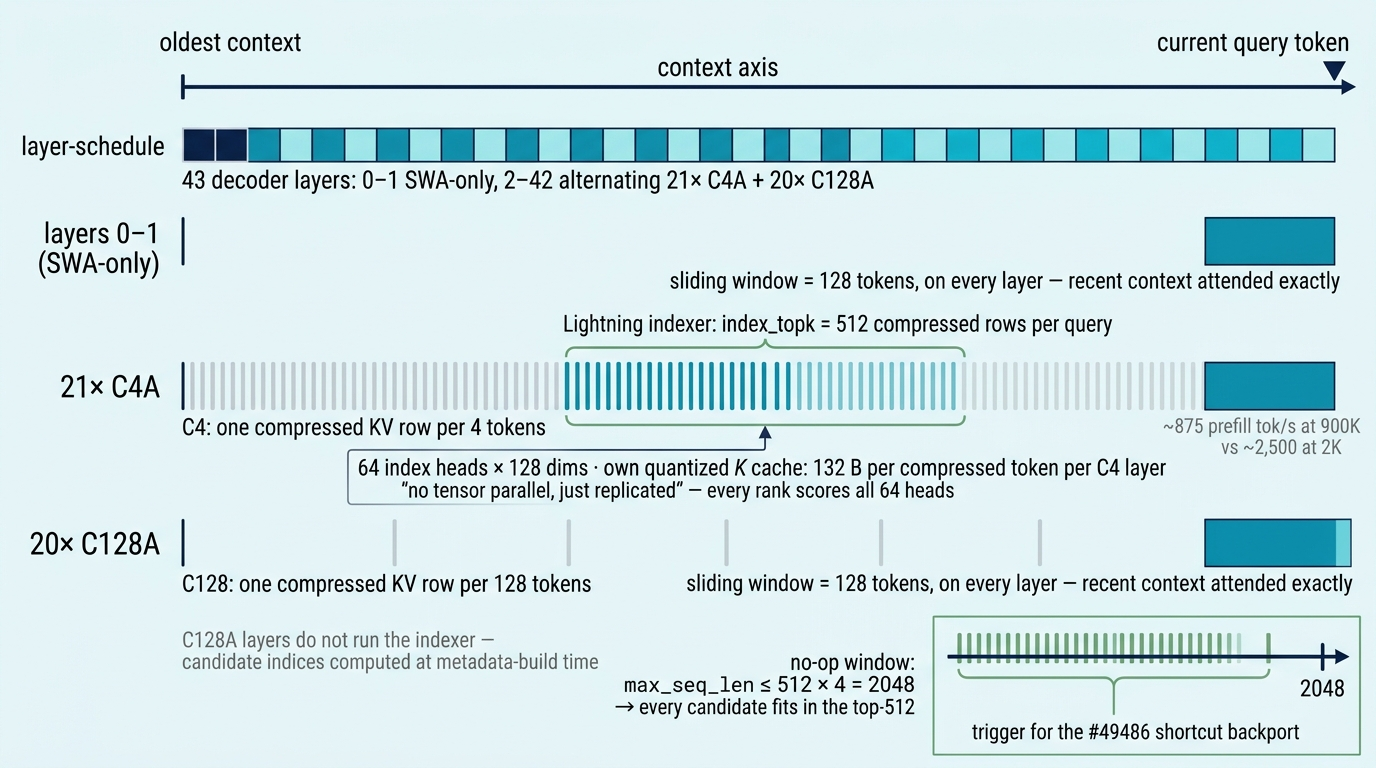
\includegraphics[width=\textwidth]{figures/ch03-attention-flavors.png}
\caption{One bargain, repeated 43 times. Every layer attends the most recent
128 tokens exactly; older context survives only as compressed rows --- one
per 4 tokens on the 21 C4A layers, one per 128 on the 20 C128A layers ---
and on C4A layers a query may read only the 512 rows the Lightning indexer
selects. Below 2{,}048 tokens every candidate already fits in the top-512,
so the selection provably cannot change the answer.}
\label{fig:attention-flavors}
\end{figure}

\subsection{The 584-byte KV row}
\label{sec:model-kvrow}

Every stored token row --- compressed or sliding-window --- occupies exactly
584 bytes, fixed by FlashInfer's \code{KVCacheTraits<DSV4>}
(\code{KV_GMEM_STRIDE = 584}). \Cref{fig:kv-row} maps the bytes.

\begin{figure}[htbp]
\centering
\begin{tikzpicture}[x=0.0235cm, y=1cm]
  % main bar
  \draw[draw=hbSteel, thick, fill=hbGreen!12] (0,0) rectangle (448,0.95);
  \draw[draw=hbSteel, thick, fill=hbBlue!8]   (448,0) rectangle (576,0.95);
  \draw[draw=hbSteel, thick, fill=hbAmber!25] (576,0) rectangle (584,0.95);
  % quant tile ticks inside NoPE region (every 64 values)
  \foreach \xx in {64,128,192,256,320,384} {
    \draw[hbSteel!50, dash pattern=on 1pt off 1pt] (\xx,0) -- (\xx,0.95);
  }
  \node at (224,0.475) {\small 448\,B NoPE: 448 $\times$ fp8 e4m3};
  \node[align=center, font=\scriptsize] at (512,0.475) {128\,B RoPE:\\64 $\times$ bf16};
  % byte offsets
  \node[hblabel, below] at (0,-0.05) {0};
  \node[hblabel, below] at (448,-0.05) {448};
  \node[hblabel, below] at (566,-0.05) {576};
  \node[hblabel, below] at (596,-0.05) {584};
  % tile brace
  \draw[decorate, decoration={brace, amplitude=4pt}, hbSteel]
    (0,1.05) -- (448,1.05)
    node[hblabel, midway, above=4pt]
    {7 quant tiles of 64 values, one UE8M0 scale each (scales live in the footer)};
  % footer zoom
  \draw[hbSteel!70] (576,0) -- (300,-1.5);
  \draw[hbSteel!70] (584,0) -- (584,-1.5);
  \draw[draw=hbSteel, thick, fill=hbAmber!25] (300,-2.3) rectangle (584,-1.5);
  \foreach \i in {1,...,6} {
    \draw[hbSteel] ({300+\i*35.5},-2.3) -- ({300+\i*35.5},-1.5);
  }
  \draw[hbSteel, thick] ({300+7*35.5},-2.3) -- ({300+7*35.5},-1.5);
  \foreach \i/\lbl in {0/S0,1/S1,2/S2,3/S3,4/S4,5/S5,6/S6} {
    \node[font=\scriptsize] at ({300+\i*35.5+17.7},-1.9) {\lbl};
  }
  \node[font=\scriptsize] at ({300+7*35.5+17.7},-1.9) {pad};
  \node[hblabel, below] at (442,-2.4)
    {8\,B footer: 7 UE8M0 scales (uint8, exponent+127) + 1 pad byte};
\end{tikzpicture}
\caption{The 584-byte per-token KV row used by both \code{fp8_ds_mla} and
\code{nvfp4_ds_mla}: 448 fp8 e4m3 NoPE values in seven 64-value quant tiles,
64 bf16 RoPE values kept at full precision, and an 8-byte footer holding the
seven power-of-two UE8M0 tile scales plus one pad byte.}
\label{fig:kv-row}
\end{figure}

The design encodes two numerics decisions. First, only the NoPE (non-rotary)
dimensions are quantized to fp8; the 64 RoPE dimensions stay bf16, because
positional phase at million-token context is the last thing you want to
degrade. Second, the scales are UE8M0 --- pure powers of two, computed as
$2^{\lceil \log_2(\mathrm{absmax}/448) \rceil}$ and stored as
$\mathrm{exponent}+127$ in a uint8 --- so dequantization is an exponent add,
not a multiply.

\begin{hblesson}
This row is what the \ghissue{22} incident from the chapter opening was
about: \code{nvfp4_ds_mla} and \code{fp8_ds_mla} store these same 584 bytes,
and there is no 4-bit KV cache in this stack today. The lesson generalizes:
when two configuration strings are documented as byte-identical, audit every
string comparison that treats them differently. A genuine 4-bit row
($\approx$292--390\,B) is a designed-but-unbuilt future
(\repofile{docs/CLAUDE/item8-fp4-kv-design.md}); it would buy roughly
+50\,\% KV tokens.
\end{hblesson}

\subsection{Per-token byte accounting and KV groups}

This subsection is the byte ledger --- reference material, not narrative.
Skim it on first read and return when you need to size a deployment.

Because C4 layers store one row per 4 tokens and C128 one per 128, the
\emph{amortized} physical cost per context token is far below 584\,B per layer
(\Cref{tab:kv-bytes}). The allocator sees something different. vLLM's hybrid
allocator requires every KV group to use the same page size in bytes, and all
four groups land on $64 \times 584 = 37{,}376$\,B pages: one
\code{MLAAttentionSpec} group (block 256 tokens) plus three
\code{SlidingWindowMLASpec} groups (blocks 64/4/8, the latter two serving the
draft layers). The published headline ``2.33\,M tokens in 17.04\,GiB''
($\approx$7.8\,KB/token) is allocator accounting across those groups, not
physical row cost.

\begin{table}[htbp]
  \centering\small
  \caption{Physical KV bytes per context token at long context (per rank;
  TP=2 replicates everything on both ranks).}
  \label{tab:kv-bytes}
  \begin{tabular}{@{}lrl@{}}
    \toprule
    Component & Bytes/token & Derivation \\
    \midrule
    C4 compressed rows & $\approx$3.07\,KB & 21 layers $\times$ 584/4 \\
    C128 compressed rows & $\approx$0.09\,KB & 20 layers $\times$ 584/128 \\
    Indexer K cache & $\approx$0.69\,KB & 21 layers $\times$ 132/4 \\
    SWA windows & --- & per-sequence constant, $\approx$3.4\,MB/seq \\
    \bottomrule
  \end{tabular}
\end{table}

\section{DSpark speculative decoding at the model level}
\label{sec:model-dspark}

Everything to this point has described what the target stack stores and
reads; the other half of every decode step is the passenger grafted onto
it. DSpark is the checkpoint's built-in speculative decoder. Mechanically it is a
descendant of MTP (multi-token prediction), but with a twist that reshapes the
serving math. The \code{mtp.N.*} draft stages are \emph{stacked} into one
non-causal draft backbone that predicts a whole \code{dspark_block_size} = 5
token block in a single parallel pass, rather than re-running one MTP layer
per drafted token. The scheduler-facing details live in \Cref{ch:specdecode};
here is the model anatomy. That anatomy has four pieces: where the drafter's
input comes from, how many stages it actually has, what a single block pass
computes, and where its state lives. The last is the one later bugs turn on,
because that state sits outside the KV cache the engine knows how to manage.

Two of the design decisions read best as reasoning rather than inventory.
The drafter's \emph{input} is not the target's final hidden state. During
the target forward, the mHC stream state after each layer listed in
\code{dspark_target_layer_ids} is collapsed (mean over streams) and copied
into a stable-address buffer allocated outside the CUDA-graph pool, so that
captured graphs refresh it at replay; the drafter reads that concatenated
mid-stack feature buffer. And the drafter's \emph{depth} is not taken on
faith. 0731 declares \code{num_nextn_predict_layers} = 1 where Vision-Exp
declares 3, but the overlay's \code{DSparkModelSpec.from_hf_config} does
not take that field on trust: it infers the true stage count from the
contiguous \code{mtp.N.*} weight namespace, its source comment noting that
DSpark releases still report \code{num_nextn_predict_layers=1}, ``so the
weight map is the reliable source for the DSpark draft depth.'' The
transferable rule: count the
weights, not the config's claims --- a checkpoint's tensors cannot lie
about their own existence.

\begin{description}
  \item[The block pass.] \code{draft()} builds a $[B, \mathrm{block}]$ input:
  the anchor token (last accepted token) first, then noise tokens, at
  positions $\mathrm{anchor} + [0, k)$. One forward of the stacked draft
  layers produces features for every position at once.
  \item[The Markov head.] Decoding the block is left-to-right, but cheap: at
  each position the base draft logits get a low-rank bias
  $W_1[\mathrm{prev\_token}] \, W_2^{\top}$ with rank
  \code{dspark_markov_rank} = 256 --- a learned bigram correction. Both
  matrices are $129{,}280 \times 256$ bf16, 66\,MB each. Stock Anemll shards
  them tensor-parallel, which costs 12 serialized collectives per decode step
  in the six-step draft loop. The replicate-Markov-head hotfix
  (\Cref{ch:patches}) makes them plain replicated modules, because 66\,MB is
  trivially affordable next to a 128\,GB unified board.
  \item[Draft state.] The drafter's KV is \emph{not} vLLM KV cache. Each draft
  layer owns a per-request sliding window of projected target features
  (\code{main_kv_cache}); the proposer registers no KV layers and sets
  \code{block_size = 1}. This design is what made the batch-condensation bug
  of the Keys concurrency patch possible --- state keyed by batch row rather
  than request id --- covered in \Cref{ch:bugs}.
\end{description}

The launcher serves this with $k=5$ or $k=6$ speculative tokens
(\code{MTP_NUM_TOKENS}, default 6). Vision-Exp exposes a config trap.
vLLM's \code{SpeculativeConfig} requires $k$ divisible by the draft stage
count ``for MTP module reuse'' --- a rule that is meaningless for DSpark's
stacked block, but with 3 stages it forces $k = 6$, one more noise query
than the 5-token block was trained with. The opt-in, SHA-pinned
\repofile{patches/hotfix-vllm-dspark-block-k.py} exempts
\code{method="dspark"} from the rule.

\begin{lstlisting}[language=bash]
# compose argv (TP=2 lane), the model-level spec-decode knobs:
--speculative-config '{"method":"dspark",
                       "num_speculative_tokens":6,
                       "draft_sample_method":"probabilistic"}'
\end{lstlisting}

Acceptance behavior is strongly prompt-dependent, and the repository measured it
honestly. On numbered-word probes the audited healthy curve is per-position
acceptance 0.92 / 0.74 / 0.60 / 0.41 / 0.28 / 0.21 --- about 48\,\% of drafted
tokens accepted, $\approx$3.9 tokens per step at $k=6$. On natural prose the
same stack accepts only $\approx$25\,\% with position-0 agreement
0.66--0.69, and a vision-lane \code{/metrics} snapshot showed 23.7\,\%
acceptance with positions 2--5 nearly dead. Drafts are verified by the target
with rejection sampling, so acceptance moves throughput, never correctness.
\Cref{fig:dspark-block} draws one block and the decay along it.

\begin{figure}[htbp]
\centering
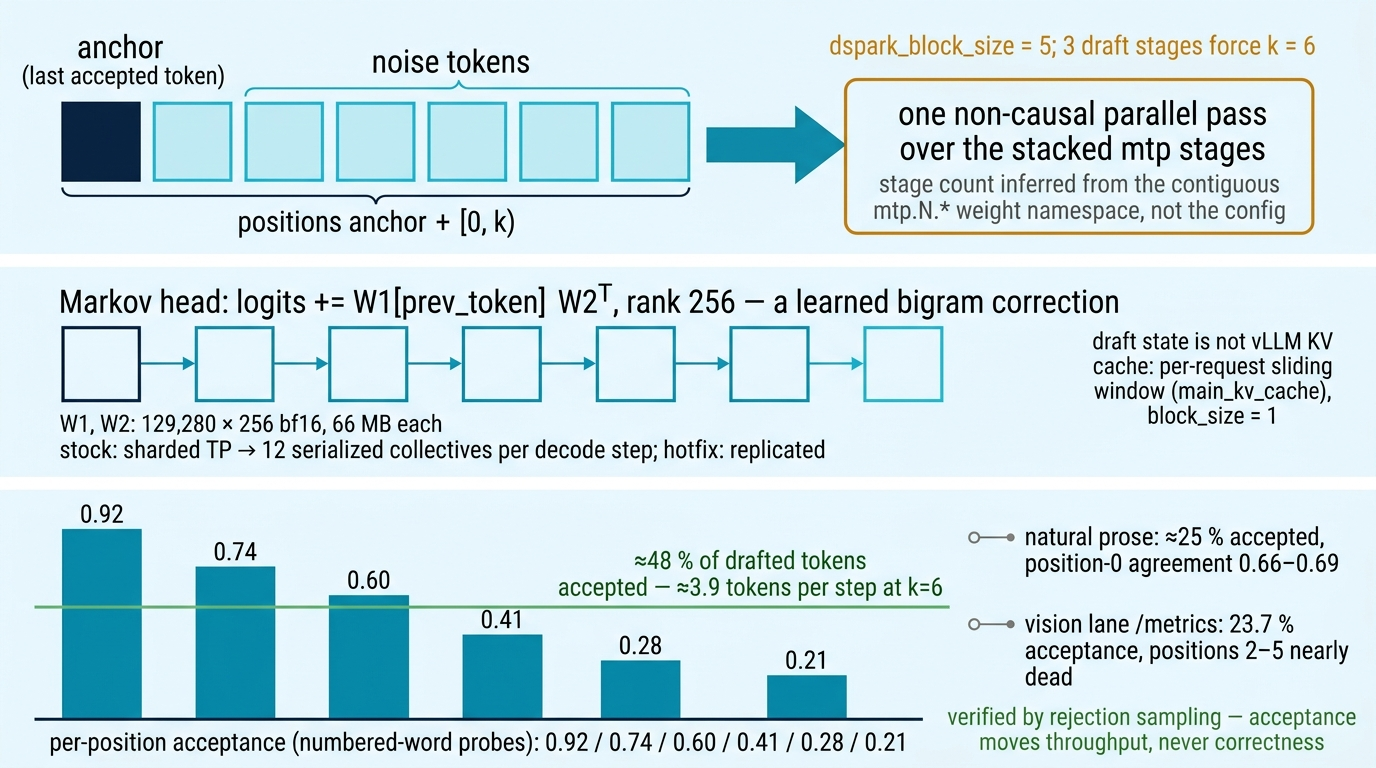
\includegraphics[width=\textwidth]{figures/ch03-dspark-block.png}
\caption{One DSpark block. The drafter builds an anchor token plus $k$ noise
tokens, produces features for all of them in a single non-causal pass, and
decodes them left-to-right through a rank-256 bigram bias; the target then
verifies the whole block in one pass. Acceptance decays steeply with position
and depends heavily on the workload --- the audited healthy curve yields
roughly 3.9 tokens per step, while natural prose and the vision lane accept
about a quarter of what is drafted.}
\label{fig:dspark-block}
\end{figure}

\section{Vision-Exp: a vision tower by startup hotfix}
\label{sec:model-vision}

The weakest of those acceptance numbers came from the vision lane --- a
lane this stack was never originally built to have.
The published 0731 checkpoint is text-only: no vision processor, projector, or
tower. DeepSeek-V4-Flash-\emph{Vision-Exp} ships a 32-layer ViT plus an
Aligner (a $3\times$ spatial downsample-and-project into the 4096-dim LLM
hidden size) and an in-vocabulary image placeholder token,
\code{<|deepseek_image|>} (token id 129{,}264).

The pinned Anemll image knows nothing about any of this, so the repository adds
vision \emph{at container start}.
\repofile{patches/hotfix-dsv4-vision-exp.py} appends a fail-closed import hook
to the stock model file, which pulls in the \repofile{patches/vision_exp/}
package and monkey-patches the three stock classes --- tower construction,
weight-name mapping, the multimodal processor, and MoE routing --- without
editing their source. Two limits are worth separating. The processor advertises support for 16
images per request, but the shipped serve flag admits only 8
(\code{--limit-mm-per-prompt} \code{{"image":8}}, \Cref{ch:profile}), so 8
is the number a client actually meets. The rest of the envelope: at most
384 LLM tokens per image (\code{vision_max_n_token}), images in \code{user}
messages only --- \code{system} and \code{assistant} return HTTP 400 --- and
no video, because the official weights have no video encoder and a GIF
decodes as a single still frame.

Two model-level mechanisms in this overlay are worth teaching, and both
follow from that bolt-on construction: the runtime underneath does not know
images exist, so each is a place where image rows must behave differently
from text rows without the surrounding machinery noticing --- the second of
them drawn in \Cref{fig:image-cache}.

\paragraph{\code{bias_vl} routing for image tokens (issue \ghissue{175}).}
Vision-Exp ships a second MoE correction bias,
\code{e_score_correction_bias_vl}, for image rows --- and image rows must skip
the hash table (an image placeholder is a real vocabulary id; looking up
\code{tid2eid[129264]} would route it like a text token). The naive
implementation scans token ids at each of the 43 gates, a GPU$\to$CPU sync per
gate. The shipped design classifies the batch once per forward (text / image /
mixed, derived from a sum the multimodal merge already reads), publishes the
verdict through the forward context, and splits mixed batches so each
partition routes with its own bias. A hard rule protects CUDA graphs: while
stream capture is active the wrapper always takes the original path, because a
captured graph must never resolve a routing kind.

\begin{hbwarstory}
\textbf{Issue \ghissue{172}: the position-dependent image block.} Vision-Exp
pads every image block so it starts on a 4-token boundary:
$4 - 1 - (\mathrm{start\_pos} \bmod 4)$ pad tokens are prepended, so the
\emph{total} block length depends on where in the prompt the image lands. A
$40\times19$ ViT grid becomes 122 core tokens plus 0--3 pad --- 122 to 125
tokens for the same pixels. vLLM's encoder cache, however, keyed entries by
content hash alone. An image first encoded at one alignment could be reused at
another, yielding ``125 placeholders vs 124 embeds'' and a scatter mismatch.
The fix salts the multimodal hash with the block's token count
(\code{salt_mm_image_hash}), bypasses the content-only processor cache for
image requests, and leaves a runtime tripwire: whenever placeholder and
embedding counts disagree, the embedding merge raises with the
\ghissue{172} explanation attached. Positional context changing the \emph{size} of an
embedded object is exactly the kind of invariant a generic cache will violate
silently.
\end{hbwarstory}

\begin{figure}[htbp]
\centering
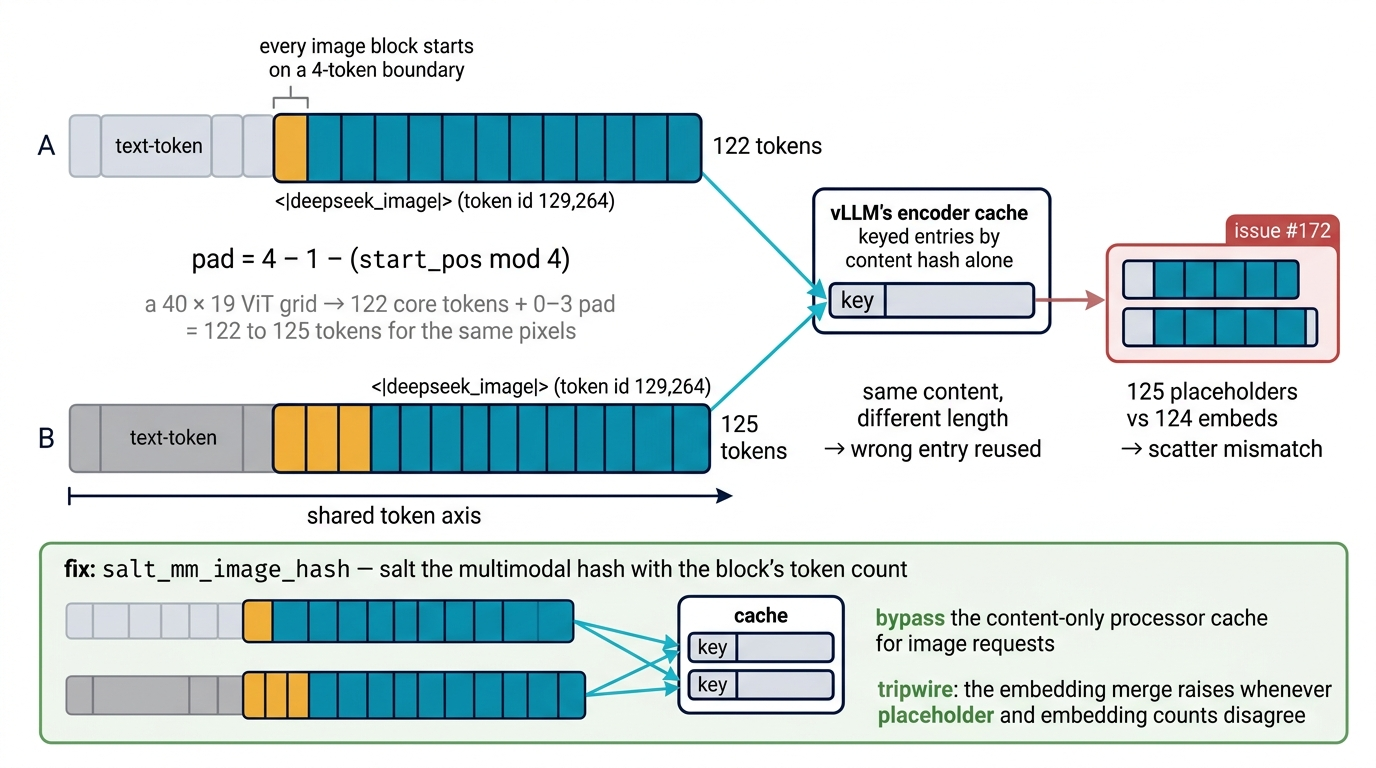
\includegraphics[width=\textwidth]{figures/ch03-image-block-cache.png}
\caption{Positional context changing the size of an embedded object.
Vision-Exp pads each image block to a 4-token boundary, so identical pixels
occupy 122 to 125 tokens depending on where the image lands in the prompt ---
while vLLM's encoder cache keyed entries by content hash alone and happily
reused an entry across alignments. Salting the hash with the block's token
count (\code{salt_mm_image_hash}) separates the two, and a runtime tripwire
catches any residual placeholder/embedding disagreement (\ghissue{172}).}
\label{fig:image-cache}
\end{figure}

\section{The encoding layer: a Python encoder instead of a chat template}
\label{sec:model-encoding}

Images, tool calls, and thinking controls all cross into and out of the
model through one last checkpoint-supplied mechanism.
The model card ships no Jinja chat template. Instead the checkpoint carries an
\code{encoding} package --- \repofile{encoding/encoding_dsv4.py} --- that
defines message rendering \emph{and} output parsing. The launcher sets
\envvar{DSPARK_ENCODING_FILE} to that file inside the container and installs
it into vLLM before import on both ranks (\code{--tokenizer-mode deepseek_v4});
request controls such as \code{chat_template_kwargs.thinking} flow through
vLLM's custom tokenizer wrapper into the Python encoder. The install also
repairs two encoder bugs: pre-0731 wrappers that mapped \code{low} reasoning
effort to \code{high}, and issue \ghissue{21}, where
\code{encode_arguments_to_dsml} only accepted JSON \emph{strings} for tool
arguments. Under \ghissue{21}, a replayed history with dict-typed arguments
was silently wrapped as \code{{"arguments": ...}}, poisoning every later
tool turn.
\Cref{fig:dsml-flow} traces the round trip.

\begin{figure}[htbp]
\centering
\adjustbox{max width=\textwidth}{%
\begin{tikzpicture}[node distance=4mm and 7mm]
  \node[hbhost, minimum width=30mm] (msgs)
    {messages JSON\\{\scriptsize roles, tools, thinking kwarg}};
  \node[hbbox, minimum width=34mm, right=of msgs] (enc)
    {encoding\_dsv4.py\\{\scriptsize renders DSML + <think>}};
  \node[hbgpu, minimum width=26mm, right=of enc] (engine)
    {vLLM engine\\{\scriptsize token ids in/out}};
  \node[hbbox, minimum width=34mm, right=of engine] (parse)
    {deepseek\_v4 parsers\\{\scriptsize reasoning + tool-call}};
  \node[hbhost, minimum width=28mm, below=8mm of parse] (out)
    {reasoning\_content\\+ tool\_calls[]};
  \draw[hbflow] (msgs) -- (enc);
  \draw[hbflow] (enc) -- (engine);
  \draw[hbflow] (engine) -- (parse);
  \draw[hbok] (parse) -- (out);
  \node[hblabel, align=center, anchor=north east]
    (dsmlfail) at ([xshift=-2mm,yshift=-8mm]parse.south west)
    {malformed DSML syntax\\$\to$ parse fails $\to$ no tool\_calls};
  \draw[hbfail] ([yshift=-1mm]parse.south west) to[bend right=15] (dsmlfail.north);
\end{tikzpicture}%
}
\caption{The encoding round trip: a checkpoint-supplied Python encoder renders
messages into DSML-marked tokens, and the paired \code{deepseek_v4} parsers
must recover structure from the output. Any syntax corruption breaks the
structured \code{tool_calls} field even when the payload was right.}
\label{fig:dsml-flow}
\end{figure}

\subsection{Thinking modes}

Reasoning effort accepts \code{off}, \code{low}, \code{high}, or \code{max};
the recipe defaults \envvar{DEFAULT_THINKING} to \code{low}, which opens a
\code{<think>} block but adds no effort instruction (matching the model's
intended base mode). \code{high}/\code{max} add instruction prefixes.

\begin{hbwarning}
\code{max_tokens} counts \emph{think plus answer}. Reasoning is generated
inside the same completion as the visible reply, so a request with
\code{DEFAULT_THINKING=max} and a small \code{max_tokens} spends the whole
window inside \code{<think>} and returns an empty-looking answer. The repository's
own benchmark notes flag this: \repofile{scripts/benchmark-0731.py} uses
natural completions without forcing \code{thinking=false}, and its numbers are
not comparable to the capped, thinking-off matrix for exactly this reason.
Budget reasoning explicitly (the per-request \code{thinking_token_budget}
parameter exists for this) rather than trusting \code{max_tokens} to bound the
visible answer.
\end{hbwarning}

\subsection{DSML tool calls and the temperature asymmetry}

Tool calls are emitted as DSML markup inside the token stream (shown here with
ASCII pipes; the real markers use a wide-bar glyph):

\begin{lstlisting}
<|DSML|tool_calls>
  <|DSML|invoke name="get_weather">
    <|DSML|parameter name="city">Paris</|DSML|parameter>
  </|DSML|invoke>
</|DSML|tool_calls>
\end{lstlisting}

The \code{deepseek_v4} tool-call parser turns this into the structured
\code{tool_calls} field of the Chat Completions response --- and it is here
that a benchmark can tell you the model got worse when it hadn't. On tool
benchmarks at temperature 1.0, the same weights score lower under this vLLM
profile than under ds4, the sibling single-Spark engine. Part of that loss is
a mechanical serving artifact rather than a model-quality signal, and
\repofile{docs/DSML_SYNTAX_TEMP_ASYMMETRY.md} documents the mechanism ---
while proposing a temperature-0 rerun to establish how much of the gap it
actually accounts for.

The asymmetry: ds4 forces \code{temperature=0} while the model emits DSML
\emph{syntax} tokens --- tags, invoke headers, JSON punctuation --- and
applies the request's sampling parameters only to argument \emph{payloads}.
vLLM has no per-region temperature mechanism: at \code{temperature=1.0}
every structural token is a full-temperature sample. A single derailed
structural token anywhere in the call makes the DSML unparseable. The
response then carries no \code{tool_calls}, and a benchmark that reads only
the structured field scores it as ``no tool call.''

The document earns its verdict by ruling out the tempting alternative
explanations (KV precision, spec decode, weight format), then lists
mitigations from cheapest to hardest. The cheapest: run tool benchmarks at
temperature 0 as a diagnostic. At the far end sit a DSML structural-tag
grammar, or a logits processor that forces argmax inside syntax regions ---
effectively porting ds4's hand-written C logic.

The generalization outlives DSML. When structure and payload are sampled at
one temperature, a benchmark that reads only the structured field is partly
scoring the decoder's syntax rather than the model's judgment.

\section{Checkpoint variants}
\label{sec:model-variants}

Like the byte ledger, this short section is reference rather than
narrative; return to it whenever two measurements disagree and you suspect
the checkpoints differ. Three checkpoint lineages appear throughout this
book; conflating them invalidates comparisons, so the repository pins them
explicitly (\Cref{tab:checkpoints}).

\begin{table}[htbp]
  \centering\footnotesize
  \caption{Checkpoint lineages served by the repository.}
  \label{tab:checkpoints}
  \begin{tabular}{@{}>{\raggedright\arraybackslash}p{3.4cm}>{\raggedright\arraybackslash}p{4.6cm}>{\raggedright\arraybackslash}p{5.6cm}@{}}
    \toprule
    Lineage & Pin & Notes \\
    \midrule
    0731 (text-only) &
    \code{deepseek-ai/DeepSeek-V4-Flash-0731} @ \code{9e165c30}\ldots &
    default \envvar{DSPARK_REVISION}; supersedes the preview
    \code{DeepSeek-V4-Flash-DSpark} checkpoint; 1 draft stage; the published
    two-Spark benchmark lane \\
    Vision-Exp (official) &
    \code{deepseek-ai/DeepSeek-V4-Flash-Vision-Exp} @ \code{86f746b3}\ldots &
    ViT + Aligner; 3 draft stages; served via the vision patch train \\
    Vision-Exp (Keys abliterated) &
    \code{drowzeys/keys-DeepSeekV4Flash-Vision-EXP-ablit}, unpinned by default
    (\envvar{DSPARK_REVISION_ABLITERATED}) &
    HF-gated; selected with \envvar{ABLITERATED}=1; applied as a 26-shard
    delta overlay onto the official snapshot \\
    \bottomrule
  \end{tabular}
\end{table}

The prepare script resolves official versus abliterated from a CLI flag, an
environment variable, or an interactive prompt, then records the choice back
into \repofile{.env.dspark}. It also guards the operational footgun: if a
pinned revision is not already in the HF cache on \emph{both} nodes, a
restart quietly becomes a $\approx$155\,GB download. Everything else in this chapter ---
architecture, KV layout, DSpark structure, encoder --- is common across the
three; what changes is the draft stage count, the vision tower, and the
weights themselves.

\FloatBarrier
The checkpoint is no longer a thing that gets loaded; it is a set of budgets
and invariants the rest of the stack negotiates with. ``17\,GiB of KV'' is a
per-rank figure the cluster pays for twice, because MLA leaves tensor
parallelism no per-head axis to cut --- the cache replicates while the
compute shards. And the names attached to those budgets are not evidence:
two KV dtypes that share every one of their 584 bytes, a config field that
misreports the drafter's stage count, a top-512 selection that provably
cannot select below 2{,}048 tokens, and a benchmark score that was partly
measuring DSML syntax rather than the model's judgment.

\section*{Takeaways}

\begin{itemize}
  \item MLA shards compute, not cache: every TP rank holds the full KV pool,
  so capacity quotes are per rank, replicated.
  \item The KV row is 584 bytes, and \code{nvfp4_ds_mla} is byte-identical
  to \code{fp8_ds_mla} --- when two config strings share bytes, audit every
  comparison that treats them differently (\ghissue{22}).
  \item DSpark predicts a whole block in one non-causal pass over
  anchor-plus-noise, decoded through a rank-256 Markov bias, with its draft
  state outside the vLLM KV cache.
  \item Layers 0--2 route MoE by token-id hash, which is why the FFN needs
  raw \code{input_ids} and image tokens need \code{bias_vl} routing that
  skips the table.
  \item Checkpoint lineage changes the draft-stage count, and the stage
  count alone changes the legal values of $k$ --- so count the weights, not
  the config's claims.
\end{itemize}

\chaptertransition{Every mechanism in this chapter reaches the running
engine as a single number or string in the launch command: the KV dtype
whose name selects a kernel, the block size the row layout implies, the
speculative $k$ the stage count constrains, the sequence count the shared
pool must absorb. None of those values is independent of the others: the
draft stage count fixes the legal $k$, and $k$ fixes the shape of every
decode step the engine has to capture. The next chapter reads
the entire \code{vllm serve} argv in that light --- the ceilings, the
KV-pool arithmetic behind the 1M claim, the thinking budgets that decide
whether an answer arrives at all --- and it opens on the smallest possible
mistake: a flag set to 42, the exactly correct product of six sequences and
$k+1$ tokens, which cost 12\,\% of six-stream throughput precisely because
nobody rounded it up.}

% =============================================================================
% Chapter 4 — The Serving Profile: Every Flag, Explained
% =============================================================================

\chapter{The Serving Profile: Every Flag, Explained}
\label{ch:profile}

The difference between passing 42 and 48 as one CUDA-graph flag was a
measured 12\,\% of six-stream throughput on this cluster: 122 versus
139~\tokspersec{} aggregate decode in an isolated A/B (2026-09-02). The
number 42 was not a mistake --- it is exactly the largest uniform decode
step at the default profile --- but unrounded it fell off the engine's
capture stride and left the busiest step running fully eager, silently.

That flag is not an outlier. A serving stack lives or dies by its launch
configuration, and this recipe's configuration is unusually load-bearing:
an empty-but-defined environment variable can silently select the wrong
RoCE GID, and a mis-set memory-utilization knob desynchronizes the two
ranks. This chapter walks through the entire profile --- every flag in the
\code{vllm serve} command that \repofile{docker-compose.dspark.yml} builds, the
KV-pool arithmetic behind the ``1M context with concurrency'' claim, the
thinking-token economy, the multimodal request contract, the three-lane
environment-variable surface, the measured workload profiles, and the API
authentication scheme.

For an inference engineer, the profile is where nearly every day-to-day
intervention happens: capacity, fairness, speculation depth, and
authentication are all set here. Several of the shipped defaults encode
hard-won fixes whose absence is invisible until load arrives. If you
operate this stack, this is the chapter to annotate.

\section{Anatomy of the vllm serve command}
\label{sec:profile-anatomy}

Both ranks run the same container command. The compose entrypoint applies the
patch train (\Cref{ch:patches}), validates a handful of inputs, then
\code{exec}s vLLM. Stripped of the shell plumbing, the effective argv at the
shipped defaults is:

\begin{lstlisting}[language=bash]
exec /usr/local/bin/vllm serve deepseek-ai/DeepSeek-V4-Flash-Vision-Exp
  --revision 86f746b36186f0e567729a5c06a8c918caba82a9
  --served-model-name deepseek-v4-flash-vision-exp
  --host 0.0.0.0 --port 8888 --trust-remote-code
  --tensor-parallel-size 2 --pipeline-parallel-size 1
  --kv-cache-dtype nvfp4_ds_mla --block-size 256
  --max-model-len 1048576 --max-num-seqs 6 --max-num-batched-tokens 8192
  --long-prefill-token-threshold 1024
  --max-cudagraph-capture-size $(( (6*(6+1)+7)/8*8 ))   # = 48
  --gpu-memory-utilization 0.835
  --enable-prefix-caching --enable-prompt-tokens-details
  --async-scheduling --enable-chunked-prefill
  --speculative-config '{"method":"dspark","num_speculative_tokens":6,"draft_sample_method":"probabilistic"}'
  --tokenizer-mode deepseek_v4 --limit-mm-per-prompt '{"image":8}'
  --distributed-executor-backend mp --moe-backend flashinfer_b12x
  --tool-call-parser deepseek_v4 --enable-auto-tool-choice
  --reasoning-parser deepseek_v4
  --default-chat-template-kwargs '{"thinking":true,"reasoning_effort":"low"}'
  --generation-config vllm --enable-flashinfer-autotune
  --nnodes 2 --node-rank 0 --master-addr <head-roce-ip> --master-port 25000
\end{lstlisting}

The worker rank runs the identical command with \code{--node-rank 1} plus
\code{--headless} (the compose template appends it via
\code{HEADLESS} expansion). Only rank~0 opens the HTTP listener on
\code{:8888}, and the container healthcheck short-circuits to success on the
headless rank, so the worker is never marked unhealthy for lacking a port.
The groups below take the flags in turn. Few of these values are free
choices: several are derived from others (the capture size from the sequence
count and $k$), several are constrained by the checkpoint ($k$ itself), and
several are the residue of an incident (the long-prefill threshold).

\subsection{Parallelism and topology}

\code{--tensor-parallel-size 2} with \code{--pipeline-parallel-size 1} shards
every layer across the two DGX Sparks; \code{--nnodes 2},
\code{--node-rank}, \code{--master-addr}, and \code{--master-port} wire the
two-process group. \code{--distributed-executor-backend mp} keeps the
in-node executor on multiprocessing. The physical NCCL/RoCE wiring underneath
is the subject of \Cref{ch:fabric}; what matters here is that the argv on both
ranks must match exactly --- the launcher syncs its private env snapshot to the
worker precisely so that both sides render the same numbers.

\subsection{KV dtype and block size}

\code{--kv-cache-dtype nvfp4_ds_mla} selects the Stage-C \emph{padded} NVFP4
sparse-MLA envelope: 584 bytes per cached row (448 fp8 NoPE + 128 bf16 RoPE +
8 scale). Despite the name, the bytes are identical to \code{fp8_ds_mla} ---
this is not the abandoned 416-byte ``true layout'' experiment, and there is no
4-bit KV saving today (\Cref{ch:patches} covers the \ghissue{22} routing fix
that exists because the two formats share bytes). \code{--block-size 256} sets
the paged-KV granularity; the separate
\envvar{VLLM_PREFIX_CACHE_RETENTION_INTERVAL} setting of 4096 is the
\ghissue{26} SWA prefix-cache spacing --- one retained window tail per
4096-token segment, plus the replay boundary.

\subsection{The three ceilings}

\code{--max-model-len 1048576} is the per-request context ceiling (1M tokens),
\code{--max-num-seqs 6} the count of simultaneously \emph{active} sequences,
and \code{--max-num-batched-tokens 8192} the prefill token budget per engine
step. All three are admission-control ceilings, not memory reservations ---
\Cref{sec:profile-kvpool} does the arithmetic. The example file's alternate
values encode the tested lanes: \code{200000} is the historical
high-concurrency profile, \code{16384} batched tokens is the big-prompt coding
profile, and \code{MAX_NUM_SEQS=16} belongs only to the Stage-C 200K path or
the TP=3 launcher.

\subsection{Chunked prefill and the long-prefill threshold}

Ceilings decide how much work is admitted; this pair decides how admitted
work shares each engine step. \code{--enable-chunked-prefill} plus
\code{--long-prefill-token-threshold 1024} is the \ghissue{27}
decode-fairness fix, and the default encodes an incident. Stock vLLM 0.25.2
defines but never enforces \code{max_num_partial_prefills}, so several
admitted-but-still-prefilling requests could each eat the full 8192-token
step budget while decode-active requests were skipped with zero new tokens
--- starvation without a single preemption. Capping each chunk at 1024
keeps every prefill chunk well under the step budget. Paired with the
\ghissue{27} hotfix that actually enforces the partial-prefill cap, it
collapsed the measured eight-stream fairness spread from ${\approx}46\times$
to ${\approx}1.05\times$; worst-case inter-token latency fell from
2{,}790\,ms to 67\,ms.

The knobs around the fix are reference matter. The companion
\envvar{DSPARK_MAX_INFLIGHT_PREFILLS} (read once by the hotfix at scheduler
construction, because Anemll 0.1.1 rejects the native CLI flag) defaults to
\code{1}: strictly serialized prefills, live-qualified after the
\ghissue{211} exact-counting fix at fairness spreads of 1.60--1.76$\times$
with zero preemptions. Values 2--3 are explicit opt-ins, and the 2026-09-02
A/B that favored 2 predates the counting fix. \code{--async-scheduling}
overlaps CPU scheduling with GPU steps and stays on by default;
\envvar{DSPARK_ASYNC_SCHEDULING}\code{=0} removes it on both ranks for the
\ghissue{191} A/B at a ${\sim}4$\,\% single-stream cost. Two settings are
forbidden:
\begin{itemize}
  \item \code{LONG_PREFILL_TOKEN_THRESHOLD=0} --- one prefill eats the
    whole batch and decode starves;
  \item \code{LONG_PREFILL_TOKEN_THRESHOLD=2048} --- measured to cost
    ${\sim}1.5$\,GB of head-node host RAM on GB10 (2026-09-02).
\end{itemize}

\subsection{The CUDA-graph capture size, and the cost of not rounding}
\label{sec:profile-capture}

The strangest-looking flag is the arithmetic one:

\begin{center}
\code{--max-cudagraph-capture-size} $=\left\lceil \frac{N_{\mathrm{seqs}}\,(k+1)}{8} \right\rceil \times 8 = 48$ \quad at $6\times(6{+}1)$.
\end{center}

A speculative decode step processes $k+1$ query tokens per sequence (six
draft positions plus the verified target token), so the largest uniform
decode step at the default profile is $6\times 7 = 42$ tokens --- the
number the opening of this chapter watched fall off the capture stride.
What the opening did not give is the mechanism. 42 is not on vLLM's default
capture stride \code{[1,2,4,8,16,24,32,40]}, so the boot log printed the
verbatim line \code{Truncating max_cudagraph_capture_size to 40}. The
spec-decode adjustment then rounded every retained size \emph{up} to a
multiple of the uniform decode query length 7 and dropped anything above
40, leaving FULL graphs \code{[7,14,21,28,35]} --- so a six-request decode
step of 42 tokens dispatched to \code{CUDAGraphMode.NONE}: fully eager,
roughly 1{,}500--1{,}800 Python-launched kernels per step. Rounding the
requested size up to a multiple of 8 yields 48. The capture list gains 48,
the rounded FULL set becomes \code{[7,14,21,28,35,42]}, and the c=6 step
replays a graph --- at the cost of about 0.1\,GiB for one extra graph
(\Cref{fig:profile-capture}).

\begin{hblesson}
The capture-size defect ran through a complete predict--fix--verify arc. A
static audit predicted the eager c=6 step from the truncation log line
alone, and the fix was a one-line compose expression. An isolated reversal
A/B (2026-09-02) measured c=6 aggregate decode at 122~\tokspersec{} with plain 42 versus
139~\tokspersec{} with padded 48 --- the truncation was costing about 12\,\%. An
earlier A/B that ``found no c=6 lift'' from capture tuning had run $k{=}5$
with a cap of 32, a configuration whose c=6 shape (36 tokens) was \emph{also}
uncaptured in both arms --- it never tested the question. Verify the boot log,
not the intention: after any change here, grep for the absence of
\code{Truncating} and for a full FULL-graph count.
\end{hblesson}

\begin{figure}[htbp]
\centering
\begin{tikzpicture}[font=\scriptsize]
  % 6x7 token grid: column 0 = verified target token, 1..6 = draft positions
  \foreach \r in {0,...,5} {
    \fill[hbGreen!35] (0,-0.45*\r) rectangle (0.38,-0.45*\r-0.38);
    \foreach \c in {1,...,6} {
      \fill[hbBlue!20] (0.45*\c,-0.45*\r) rectangle (0.45*\c+0.38,-0.45*\r-0.38);
    }
  }
  \draw[hbSteel!60] (-0.02,0.02) rectangle (3.12,-2.66);
  % braces
  \draw[decorate,decoration={brace,amplitude=4pt},color=hbSteel]
    (0,0.12) -- (3.10,0.12) node[midway,above=5pt,hblabel]
    {$k+1=7$ tokens/seq (1 verified + 6 draft)};
  \draw[decorate,decoration={brace,amplitude=4pt},color=hbSteel]
    (3.24,-2.66) -- (3.24,0.02) node[midway,right=5pt,hblabel,align=left]
    {MAX\_NUM\_SEQS\\= 6 sequences};
  % capture-size bar: 42 live + 6 pad = 48
  \fill[hbBlue!25]  (0,-3.55) rectangle (4.2,-3.15);
  \fill[hbSteel!30] (4.2,-3.55) rectangle (4.8,-3.15);
  \draw[hbSteel] (0,-3.55) rectangle (4.8,-3.15);
  \node at (2.1,-3.35) {42 live step tokens};
  \node[hblabel,anchor=north] at (2.4,-3.62) {+6 pad $\rightarrow$ capture size 48 (multiple of 8)};
  % outcomes
  \node[hbnode,fill=hbGreen!12,draw=hbGreen!70!black,align=left,anchor=north west,
        text width=6.6cm] (ok) at (7.4,0.0)
    {\textbf{Padded 48:} capture list gains 48; FULL graphs
     rounded to multiples of 7: [7,14,21,28,35,42];
     the c=6 step replays a graph.};
  \node[hbwarn,align=left,anchor=north west,text width=6.6cm]
        (bad) at ($(ok.south west)+(0,-0.3)$)
    {\textbf{Plain 42:} ``Truncating max\_cudagraph\_capture\_size to 40''
     $\rightarrow$ FULL graphs [7,14,21,28,35]; the 42-token step runs
     eager: c=6 aggregate 122 vs 139 tok/s ($-12\%$).};
  \draw[hbok]   (4.8,-3.2) .. controls (7.1,-3.0) and (7.3,-1.2) .. (ok.west);
  \draw[hbfail] (4.2,-3.5) .. controls (6.4,-3.9) and (7.0,-2.9) .. (bad.west);
\end{tikzpicture}
\caption{The uniform decode step at the default profile:
$6$ sequences $\times$ $(k{+}1)=7$ tokens $=42$ live tokens per step. Passing
the plain product as the capture size loses the shape to truncation and
rounding; padding to the next multiple of 8 keeps the c=6 step on a FULL CUDA
graph.}
\label{fig:profile-capture}
\end{figure}

\subsection{The speculative config}

The $k$ that shaped the capture arithmetic is set here --- and it is less
free to vary than it looks.
\code{--speculative-config} carries a JSON blob assembled by the entrypoint:

\begin{lstlisting}[language=jsonhb]
{"method":"dspark","num_speculative_tokens":6,"draft_sample_method":"probabilistic"}
\end{lstlisting}

\envvar{MTP_NUM_TOKENS} (default 6) becomes \code{num_speculative_tokens},
and Vision-Exp constrains it twice. The checkpoint's
\code{dspark_block_size} is 5, and $k<5$ silently truncates draft blocks on
the pinned Anemll image; with \code{num_nextn_predict_layers}\,$=3$,
vLLM's MTP module-reuse rule additionally requires $k$ divisible by 3. The
smallest legal $k$ is therefore 6 --- the trap being that the 0731 text
checkpoint (\code{n_predict}\,$=1$) happily booted the trained $k{=}5$. The
opt-in \envvar{DSPARK_ENABLE_DSPARK_BLOCK_K} hotfix drops the divisibility
rule so $k{=}5$ can run (capture $6\times 6 \rightarrow 40$).

\envvar{DRAFT_SAMPLE_METHOD} defaults to \code{probabilistic}, the value
this compose historically hardcoded; the official model cards pair
\code{greedy} with $k{=}7$ (\ghissue{84}), which also fails the Vision-Exp
divisibility check. The entrypoint accepts exactly \code{probabilistic} or
\code{greedy} and exits 2 on anything else, so an unvalidated string can
never reach the JSON. \Cref{ch:specdecode} covers what DSpark does with
these tokens.

\subsection{Binding the model: parsers, backend, generation config}

The remaining flags are flag-to-effect reference.
\code{--tokenizer-mode deepseek_v4} selects the custom tokenizer (whose
\repofile{encoding/encoding_dsv4.py} the entrypoint copies out of the
checkpoint snapshot at boot); \code{--tool-call-parser deepseek_v4} with
\code{--enable-auto-tool-choice} turns DSML tool markup into OpenAI
\code{tool_calls}; \code{--reasoning-parser deepseek_v4} plus the
\code{--reasoning-config} JSON (\code{<think>}\,/\,\code{</think>}
delimiters) separates reasoning from visible content.
\code{--default-chat-template-kwargs} is rendered from
\envvar{DEFAULT_THINKING} (\Cref{sec:profile-thinking}); a request-level
\code{chat_template_kwargs} still wins.

\code{--moe-backend flashinfer_b12x} routes the 256-expert MoE through the
B12X kernels (W4A16 on this checkpoint; \Cref{ch:perf}), with
\code{--enable-flashinfer-autotune} running the tactic search at boot
against a persisted cache. \code{--generation-config vllm} is deliberate
minimalism --- no sampling override, so vLLM's neutral defaults apply and
explicit client parameters always win. \code{--enable-prefix-caching}
plus \code{--enable-prompt-tokens-details} turn on prefix reuse and the
\code{cached_tokens} usage field that lets clients observe it.

\section{KV pool arithmetic: ceilings versus reservations}
\label{sec:profile-kvpool}

Not every default encodes an incident; some encode arithmetic --- and the
KV pool's is the arithmetic most often gotten wrong. The headline ``1M
context, six concurrent sequences'' invites a wrong mental
model: six reservations of 1M tokens each. Nothing is reserved.
After weights load, vLLM sizes one shared pool of 256-token KV blocks from
what remains under the memory-utilization target, and both
\code{max_model_len} and \code{max_num_seqs} are pure admission ceilings. The
only hard constraint is
$\sum(\text{live tokens}) \le \text{KV pool}$, enforced block-by-block as
sequences grow; when the pool runs out, new work queues and running sequences
can be preempted. The distinction worth carrying out of this chapter is
between the flags and the pool: the capacity flags are admission ceilings,
and the pool is the only thing actually spent --- one shared allocation of
blocks, drawn down by whatever happens to be live. \Cref{fig:profile-kvpool} and
\Cref{tab:profile-kvmath} give the shipped cluster's numbers.

\begin{figure}[htbp]
\centering
\begin{tikzpicture}[font=\small]
  \node[hbtitle] at (5.5,3.85) {Shared KV pool: 2{,}331{,}430 tokens (17.04 GiB, util 0.83)};
  % ceiling bracket (1,048,576 of 2,331,430 ~ 4.95cm of 11cm)
  \draw[decorate,decoration={brace,amplitude=4pt},color=hbAmber!80!black]
    (0,2.55) -- (4.95,2.55) node[midway,above=5pt,hblabel,align=center]
    {per-request \emph{ceiling}: max\_model\_len = 1{,}048{,}576\\a limit, not a reservation};
  % pool
  \draw[draw=hbSteel,thick,rounded corners=2pt] (0,1.2) rectangle (11,2.0);
  \fill[hbBlue!30]   (0.05,1.25) rectangle (2.85,1.95);
  \fill[hbGreen!30]  (2.90,1.25) rectangle (4.30,1.95);
  \fill[hbAmber!35]  (4.35,1.25) rectangle (4.90,1.95);
  \fill[hbAccent!25] (4.95,1.25) rectangle (5.20,1.95);
  \node at (1.45,1.6) {\scriptsize seq 1: 600K};
  \node at (3.60,1.6) {\scriptsize seq 2: 300K};
  \node[hblabel,anchor=north] at (4.62,1.18) {seq 3: 120K};
  \node[hblabel,anchor=south] at (5.35,2.02) {seq 4: 50K};
  \node[hblabel] at (8.1,1.6) {free 256-token blocks};
  % queued request
  \node[hbfaint,anchor=west,font=\scriptsize] (q) at (8.0,0.45) {seq 7: waiting (max\_num\_seqs = 6 active)};
  \draw[hbfail,dashed] (q.west) -- (7.6,1.25);
  \node[hblabel,anchor=west,align=left,text width=7.2cm] at (0,0.35)
    {admission rule: $\sum(\text{live tokens}) \leq$ pool; sequences grow block-by-block and queue when blocks run out};
\end{tikzpicture}
\caption{Ceilings versus reservations. Live sequences of very different
lengths draw blocks from one shared pool; \code{max_model_len} bounds any one
of them and \code{max_num_seqs} bounds how many are active, but neither
reserves memory.}
\label{fig:profile-kvpool}
\end{figure}

\begin{table}[htbp]
\centering\small
\caption{Six concurrent sequences against the 2{,}331{,}430-token pool.}
\label{tab:profile-kvmath}
\begin{tabular}{@{}lrl@{}}
\toprule
Scenario & Total live tokens & Verdict \\
\midrule
$6 \times 50\mathrm{K}$  & 300K & easy \\
$6 \times 200\mathrm{K}$ & 1.2M & fits \\
$6 \times 500\mathrm{K}$ & 3.0M & near/over pool --- some queue \\
$6 \times 1\mathrm{M}$   & 6.0M & impossible --- extras queue \\
\bottomrule
\end{tabular}
\end{table}

The numbers to trust are the ones the engine prints at boot, on this cluster:

\begin{lstlisting}
Available KV cache memory: 17.04 GiB
GPU KV cache size: 2,331,430 tokens
Maximum concurrency for 1,048,576 tokens per request: 2.22x
\end{lstlisting}

The \code{2.22x} line answers only one narrow question --- how many
\emph{simultaneous full-1M} requests fit --- and is not a concurrency limit
for normal traffic. Note also that these numbers are per-deployment facts, not
constants: the text-only 0731 checkpoint boots at 18.08\,GiB /
2{,}493{,}464 tokens / 2.38$\times$ (that boot recorded at
\envvar{GPU_MEMORY_UTILIZATION_TEXT}\,=\,0.835 against the reference boot's
0.83), because the Vision-Exp ViT and aligner consume more weight memory. And because vLLM sizes
the pool from the \emph{minimum} across ranks, host-memory bloat on the worker
alone shrinks the pool on both nodes (\Cref{ch:operations}).

\begin{hbwarning}
Never set \envvar{GPU_MEMORY_UTILIZATION} by hand. The launcher exports it
from \envvar{GPU_MEMORY_UTILIZATION_TEXT} (shipped default 0.835; the
reference boot above was recorded at 0.83), and the same derived value is
written into the env snapshot the worker consumes. A hand-set value on one
node desynchronizes the ranks or silently overrides the profile. The same
rule applies to \envvar{DSPARK_MODEL}, which start and prepare resolve from
the \envvar{ABLITERATED} flag. If CUDA-graph capture OOMs, lower
\envvar{GPU_MEMORY_UTILIZATION_TEXT} toward ${\sim}0.78$; raising it grows
the KV pool at roughly $+1.2$\,GiB (${\approx}165$K tokens) per $+0.01$, but
only after host memory pressure is dealt with.
\end{hbwarning}

\section{Thinking and token budgets}
\label{sec:profile-thinking}

The thinking defaults encode a support-ticket shape: an answer that comes
back empty because reasoning silently ate the budget. Reasoning is best
treated as spending rather than as a mode: it draws on the same
\code{max_tokens} the visible answer needs, and only
\code{thinking_token_budget} divides the two.
\envvar{DEFAULT_THINKING} sets the server-wide default reasoning mode; the
entrypoint maps it onto \code{--default-chat-template-kwargs}
(\Cref{tab:profile-thinking}), any other value exits 2, and a request-level
\code{chat_template_kwargs} always overrides.

\begin{table}[htbp]
\centering\footnotesize
\caption{\envvar{DEFAULT_THINKING} levels and their rendered template kwargs.}
\label{tab:profile-thinking}
\begin{tabular}{@{}ll>{\raggedright\arraybackslash}p{4.2cm}@{}}
\toprule
Level & Rendered kwargs & Notes \\
\midrule
\code{off}  & \code{{"thinking":false}} & no \code{<think>} block \\
\code{low}  & \code{{"thinking":true,"reasoning_effort":"low"}} & shipped default \\
\code{high} & \code{{"thinking":true,"reasoning_effort":"high"}} & \\
\code{max}  & \code{{"thinking":true,"reasoning_effort":"max"}} & ${\sim}3\times$ per-request latency vs \code{low} (measured) \\
\bottomrule
\end{tabular}
\end{table}

The economic fact clients must internalize: \code{max_tokens} counts
\emph{think plus answer} --- reasoning, visible response, and tool markup all
draw from one budget. At \code{DEFAULT_THINKING=max} the checkpoint ships a
directive not to stop reasoning until ``no error remains undiscovered,'' and
live measurement on a moderate prompt produced roughly 50{,}000 reasoning
characters (${\approx}12{,}500$ tokens). A harness cap of 256/512/800 tokens
therefore commonly returns \code{content: null} with
\code{finish_reason: length}, because reasoning ate the entire budget before
the answer began. ``Size \code{max_tokens} accordingly'' means tens of
thousands of tokens, not a small bump. Inspect \code{finish_reason} and
\code{completion_tokens} on every response: \code{length} plus null content
means think ate the cap (\Cref{fig:profile-tokenbudget}).

The precise tool for this problem is \code{thinking_token_budget}, which caps
only the reasoning portion, forces a single \code{</think>} at the boundary,
and leaves the rest of \code{max_tokens} for the visible answer (a budget of
0 disables reasoning for that request). But the field is \defoff{} twice over
(\ghissue{31}, \ghissue{66}). Stock V2 rejects it with HTTP~400, so the
server must boot with \envvar{DSPARK_ENABLE_ISSUE31_GPU_HOTFIX}\code{=1}
(fail-closed patch, containers recreated); even then the server injects no
default --- each request must send the field explicitly. Leave the flag at 0
unless a client actually sends the field; \ghissue{66} documents a decode
cliff risk for omit-field traffic with the patch enabled. A typical
budgeted request:

\needspace{5\baselineskip}
\begin{lstlisting}[language=jsonhb]
{
  "max_tokens": 4096,
  "thinking_token_budget": 1024,
  "temperature": 0.6, "top_p": 0.95,
  "chat_template_kwargs": {"thinking": true, "reasoning_effort": "high"}
}
\end{lstlisting}

\begin{figure}[htbp]
\centering
\adjustbox{max width=\textwidth}{%
\begin{tikzpicture}[font=\scriptsize]
  % ============ heading ============
  \node[hbtitle, anchor=west] at (0,9.40)
    {\texttt{max\_tokens} counts think plus answer};

  % ============ bar 1 : no budget, reasoning overruns ============
  \node[anchor=south west, font=\scriptsize] at (0,8.52)
    {harness cap of 256 / 512 / 800 tokens};
  \fill[amber!45] (0,7.90) rectangle (1.95,8.45);
  \draw[navy, thick] (0,7.90) rectangle (1.95,8.45);
  \draw[hbfail, line width=1pt] (1.95,8.175) -- (4.80,8.175);
  \node[hbwarn, anchor=west, font=\scriptsize, inner sep=4pt] at (5.05,8.175)
    {content: null $\cdot$ finish\_reason: length};
  \node[hblabel, anchor=north west, align=left, text width=11.3cm] at (0,7.70)
    {\texttt{DEFAULT\_THINKING=max}: ``no error remains undiscovered''\\
     measured on a moderate prompt: \textasciitilde50{,}000 reasoning
     characters ($\approx$12{,}500 tokens)};

  % ============ bar 2 : budgeted split ============
  \node[anchor=south west, font=\scriptsize] at (0,6.28)
    {\texttt{max\_tokens: 4096} $\cdot$ \texttt{thinking\_token\_budget: 1024}};
  \fill[amber!45] (0,5.62) rectangle (2.50,6.17);
  \fill[teal!25]  (2.50,5.62) rectangle (10.0,6.17);
  \draw[navy, thick] (0,5.62) rectangle (10.0,6.17);
  \draw[navy, line width=1.4pt] (2.50,5.30) -- (2.50,6.17);
  \node[hblabel, anchor=north west] at (2.66,5.38)
    {forces a single \texttt{\textless/think\textgreater} at the boundary};

  % ============ bar 3 : budget 0 ============
  \node[anchor=south west, font=\scriptsize] at (0,4.38)
    {budget 0 disables reasoning for that request};
  \fill[teal!25] (0,3.72) rectangle (10.0,4.27);
  \draw[navy, thick] (0,3.72) rectangle (10.0,4.27);

  % ============ gating strip ============
  \node[hbpatch, anchor=north west, align=left, font=\scriptsize,
        text width=6.0cm] (gate) at (0,3.28)
    {doubly opt-in: \texttt{DSPARK\_ENABLE\_ISSUE31\_GPU\_HOTFIX=1} (\#31)
     AND the per-request field};
  \node[hbwarn, anchor=north west, align=left, font=\scriptsize,
        text width=6.4cm] (nA) at (8.0,3.28)
    {stock V2 rejects the field with HTTP 400};
  \node[hbwarn, anchor=north west, align=left, font=\scriptsize,
        text width=6.4cm] (nB) at (8.0,2.36)
    {mismatch: ``\texttt{thinking\_token\_budget} is not yet supported by
     the V2 model runner''};
  \draw[hbfail] (gate.east) to[out=25,in=180] (nA.west);
  \draw[hbfail] (gate.east) to[out=-25,in=180] (nB.west);

  % ============ side panel ============
  \node[hbfaint, anchor=north west, align=left, font=\scriptsize,
        text width=4.6cm] at (10.7,9.30)
    {pi defaults: minimal 1024 / low 2048 / medium 8192 / high 16384};
  \node[hbfaint, anchor=north west, align=left, font=\scriptsize,
        text width=4.6cm] at (10.7,6.30)
    {max $\approx$3$\times$ per-request latency vs low (measured)};

  % ============ bottom markers ============
  \node[hbpatch, anchor=north west, align=left, font=\scriptsize,
        text width=6.6cm] at (0,1.12)
    {stop strings stay dormant inside \texttt{\textless think\textgreater}
     (\texttt{DSPARK\_SUPPRESS\_STOPS\_IN\_REASONING=1})};
  \node[hbpatch, anchor=north west, align=left, font=\scriptsize,
        text width=6.4cm] at (8.0,1.12)
    {\#66: decode cliff risk for omit-field traffic with the patch enabled};
\end{tikzpicture}%
}
\caption{One budget, two consumers. Reasoning and the visible answer are
generated inside the same completion and drawn from the same
\code{max_tokens}: at \code{DEFAULT_THINKING=max} a moderate prompt produced
roughly 12{,}500 tokens of reasoning, so a harness cap of a few hundred
returns \code{content: null} with \code{finish_reason: length}.
\code{thinking_token_budget} is the only mechanism that divides the two ---
and it is opt-in at boot and again per request.}
\label{fig:profile-tokenbudget}
\end{figure}

\begin{hbnote}
The boot flag pairs with a client capability. The shipped
\repofile{pi-models.dspark.example.json} sets
\code{supportsThinkingTokenBudget: false} to match the server default; once
the boot flag is 1, flipping that capability makes the pi client attach a
\code{thinking_token_budget} whenever thinking is enabled, sized from
per-level defaults (\code{minimal} 1024 / \code{low} 2048 / \code{medium}
8192 / \code{high} 16384) and always leaving room for the answer. Mismatched
halves fail loudly: capability \code{true} against boot flag 0 makes every pi
request fail with ``\code{thinking_token_budget} is not yet supported by the
V2 model runner.''
\end{hbnote}

Two related guards from the patch train complete the picture. Client
\code{stop} strings stay dormant inside \code{<think>} until \code{</think>}
(\envvar{DSPARK_SUPPRESS_STOPS_IN_REASONING}\code{=1} by default --- without
it, a stop string firing mid-reason yields blank \code{content}). And a tool
call truncated by \code{max_tokens} reports \code{finish_reason: "length"}
with non-parseable arguments dropped, instead of poisoning the transcript
with invalid JSON under \code{finish_reason: "tool_calls"} (\ghissue{55},
\Cref{ch:patches}).

\section{Multimodal request rules}
\label{sec:profile-multimodal}

The multimodal rules encode an incident too: one misplaced image can poison
an entire agent session. Vision-Exp accepts OpenAI \code{image_url} parts
(JPEG/PNG/GIF/WebP; GIF is a still frame, and there is no video encoder in
the official weights) --- but only on \code{user} messages. A structured \code{image}\,/\,\code{image_url}
part, or the raw image token, on a \code{system}, \code{assistant},
\code{tool}, or \code{function} message returns HTTP~400. Tool \emph{text}
that merely quotes \code{<image>} tags is allowed; a vision-tool result
delivered as \code{image_url} on \code{role: "tool"} is not. Put screenshots
on a \code{user} turn.

\begin{hbwarstory}
The 400 is worse than a failed request (\ghissue{178}). Typical OpenAI
clients do not retry a 400, and --- crucially --- the rejected turn stays in
the client's conversation history. Every subsequent request replays the same
malformed tool message and fails the same way: one misplaced screenshot
converts an agent session into a permanent failure loop until the offending
tool message is dropped from history. The trap earns its own defensive rule
in harness design: validate where images land \emph{before} appending them to
the transcript.
\end{hbwarstory}

The per-request cap is \envvar{LIMIT_MM_PER_PROMPT}, default
\code{{"image":8}}. Anemll's argparse accepts only JSON here
(\code{json.loads}), so the entrypoint converts the friendlier
\code{image=N} spelling to \code{{"image":N}} and exits 2 if $N$ is not a
plain integer --- a small example of the profile's general pattern of
normalizing operator input before it reaches vLLM.

\section{The environment-variable surface: three lanes}
\label{sec:profile-envs}

In the environment surface the incidents are subtler: variables that do
nothing while looking load-bearing, and one that does the wrong thing while
looking absent. The repository carries dozens of environment variables, and
\repofile{docs/ENVS.md} sorts them into three lanes by an audited criterion:
whether the key is registered in \code{vllm.envs.environment_variables}
inside the default Anemll 0.1.1 image (audit date 2026-07-29, re-run the
in-container snippet after image bumps).

\begin{table}[htbp]
\centering\footnotesize
\caption{The three environment-variable lanes of \repofile{docs/ENVS.md}.}
\label{tab:profile-envlanes}
\begin{tabular}{@{}>{\raggedright\arraybackslash}p{3.4cm}>{\raggedright\arraybackslash}p{5.4cm}>{\raggedright\arraybackslash}p{5.6cm}@{}}
\toprule
Lane & Examples & Behavior on Anemll 0.1.1 \\
\midrule
A. Anemll-safe (registered \code{VLLM_*} or non-\code{VLLM_} runtime) &
\envvar{VLLM_USE_BREAKABLE_CUDAGRAPH}, \envvar{VLLM_EXECUTE_MODEL_TIMEOUT_SECONDS}, \envvar{CUTE_DSL_ARCH}, \envvar{TRITON_CACHE_DIR}, \envvar{NCCL_*} &
Consumed as intended by vLLM or the runtime libraries. \\
\addlinespace
B. Stage-C-only &
\envvar{VLLM_DSPARK_GPU_REJECTED_CONTEXT_MASK}, \envvar{VLLM_DSPARK_LOCAL_ARGMAX}, \envvar{VLLM_DSV4_B12X_COMPRESSED_MLA} &
Warn-and-ignore no-ops; meaningful only on the Stage-C image with \repofile{docker-compose.stage-c.override.yml} merged. \\
\addlinespace
C. Launcher / compose only &
\envvar{DSPARK_MODEL}, \envvar{DSPARK_REVISION}, \envvar{DSPARK_VLLM_IMAGE}, \envvar{VLLM_HOST}, \envvar{VLLM_PORT}, \envvar{DSPARK_BOOT_SHAPE_WARMUP}, \envvar{DSPARK_WORKER_HF_NFS}, \envvar{HF_TOKEN} &
Consumed by start scripts or compose substitution, never by the serving process (\envvar{HF_TOKEN} reaches only the prepare container). \\
\bottomrule
\end{tabular}
\end{table}

The warning semantics matter for debugging. vLLM validates any process env key
starting with \code{VLLM_}; an unknown key logs
\code{Unknown vLLM environment variable detected: VLLM_...} and is
\emph{ignored} --- the serve still starts. Two inferences are therefore
invalid. An unknown-env warning does not mean the corresponding logic is
absent (DSpark and the Keys concurrency work may be baked into the image
without exposing every Stage-C kill-switch), and setting a Stage-C-only key on
Anemll does not enable anything. Setting
\envvar{VLLM_DSPARK_GPU_REJECTED_CONTEXT_MASK}\code{=1} on the default image
is a documented no-op --- which is exactly why the published 315/205~\tokspersec{}
200K-16 numbers cannot be reproduced by flipping envs on the Anemll lane
(\Cref{ch:measurement}).

\Cref{fig:profile-configflow} traces how a value travels from the operator's
file to the serving argv, and where each normalization happens. The
defined-empty contract in the entrypoint deserves its own explanation. A
compose \code{environment:} map cannot conditionally omit a key, so every
mapped knob arrives in the container \emph{defined}, possibly empty. For
most variables that is harmless; for the NCCL passthrough keys it is not,
because NCCL loads config-file values (\repofile{/etc/nccl.conf},
\envvar{NCCL_CONF_FILE}) with overwrite disabled --- a defined-but-empty
process variable would silently mask them.

One key hides the chapter's nastiest trap, so state the rule first: to
NCCL, \emph{defined-empty is not absent --- it is a value}.
\envvar{NCCL_IB_GID_INDEX} parses a defined-empty setting as GID index 0,
the \code{fe80} link-local entry --- precisely when the launcher's GID auto
mode deliberately leaves the variable empty so that NCCL selects the
RoCEv2/IPv4 GID per HCA. An empty variable that was meant to mean ``choose
well'' would instead silently select the one GID nobody wants.

The entrypoint therefore \code{unset}s every empty passthrough key
(\envvar{NCCL_IB_MERGE_NICS}, \envvar{NCCL_IB_SUBNET_AWARE_ROUTING},
\envvar{NCCL_IB_SUBNET_PREFIX_LEN}, \envvar{NCCL_NET_GDR_LEVEL},
\envvar{NCCL_NET_GDR_READ}, \envvar{NCCL_DMABUF_ENABLE},
\envvar{NCCL_IB_GID_INDEX}) before \code{exec}. Configured non-empty values
pass through unchanged, and an empty value is normalized to truly absent ---
by design, the mechanism cannot be used to force an empty setting.

\begin{figure}[htbp]
\centering
\begin{tikzpicture}[node distance=5.5mm,font=\small]
  \node[hbhost,text width=11.6cm,align=left] (env)
    {\textbf{1. \texttt{.env.dspark}} --- operator intent: MAX\_NUM\_SEQS,
     MTP\_NUM\_TOKENS, GPU\_MEMORY\_UTILIZATION\_TEXT, NCCL\_* wiring,
     ABLITERATED, auth keys};
  \node[hbbox,below=of env,text width=11.6cm,align=left] (launcher)
    {\textbf{2. Launcher \texttt{start-deepseek-v4-flash-dspark.sh}} ---
     sources the file; validates the numeric knobs (integer, bounded, decimal-normalized);
     derives GPU\_MEMORY\_UTILIZATION from \_TEXT and DSPARK\_MODEL from
     ABLITERATED; resolves GIDs; syncs one normalized env snapshot to the worker};
  \node[hbbox,below=of launcher,text width=11.6cm,align=left] (compose)
    {\textbf{3. Compose interpolation} (\texttt{docker-compose.dspark.yml}) ---
     \$\{VAR:-default\} fills defaults; every mapped key is \emph{defined} in
     the container, so unconfigured knobs arrive empty rather than absent};
  \node[hbpatch,below=of compose,text width=11.6cm,align=left] (entry)
    {\textbf{4. Container entrypoint} --- unsets defined-empty NCCL passthrough
     keys; validates DRAFT\_SAMPLE\_METHOD and the API-key variables (exit 2);
     builds the speculative-config and limit-mm JSON; computes the padded
     capture size; applies the patch train fail-closed};
  \node[hbgpu,below=of entry,text width=11.6cm,align=left] (vllm)
    {\textbf{5. \texttt{exec /usr/local/bin/vllm serve} argv} --- identical on
     both ranks; rank 1 adds \texttt{--headless}};
  \draw[hbflow] (env) -- (launcher);
  \draw[hbflow] (launcher) -- (compose);
  \draw[hbflow] (compose) -- (entry);
  \draw[hbflow] (entry) -- (vllm);
\end{tikzpicture}
\caption{The configuration pipeline. Each stage normalizes what the next
consumes; the entrypoint's unset-if-empty pass exists because compose cannot
omit a mapped key and NCCL treats defined-empty differently from absent.}
\label{fig:profile-configflow}
\end{figure}

\section{Workload profiles}
\label{sec:profile-workloads}

The profiles are where ``defaults encode incidents'' becomes literal: every
row of the table below is a tested configuration, and one carries an
unresolved stall. Three tuned profiles cover the tested workload space
(\Cref{tab:profile-workloads}); everything else in the example file is either
cluster wiring or an opt-in hotfix.

\begin{table}[htbp]
\centering\footnotesize
\caption{Tuned serving profiles. All keep the 1M context ceiling.}
\label{tab:profile-workloads}
\footnotesize
\begin{tabular}{@{}lrrr>{\raggedright\arraybackslash}p{4.6cm}@{}}
\toprule
Profile & seqs & batched tok & util & Measured character \\
\midrule
Default agent (shipped) & 6 & 8{,}192 & 0.835 & 62--83 \tokspersec{} c=1; ${\sim}$160--190 agg.\ at c=6 short \\
Big-prompt coding & 4 & 16{,}384 & 0.87 & larger prefill chunks per step \\
Raised admission & 32 & 12{,}288 & 0.835 & c=32 325 agg.\ --- see stability caveats \\
\bottomrule
\end{tabular}
\end{table}

The raised-admission block in \repofile{.env.dspark.example} is a model of
the repository's honesty discipline, and the honesty is operationally load-bearing.
The performance side, measured at 2$\times$ DGX Spark TP=2 on bursts that
completed (short prompts, thinking low, 500-token generations):
c=1 47--54 \tokspersec{}, c=8 154, c=16 213, c=32 \textbf{325 aggregate}, versus a
baseline where c=8 queued above the admission cap at ${\sim}108$. Two knobs
move together: at $k{=}6$, raised admission consumes the 8192 budget with
draft slots (the engine warns \code{max_num_scheduled_tokens is set to ...}),
costing single-stream decode; 12{,}288 recovers it fully. And raising
admission does \emph{not} require dropping the context ceiling: the KV pool is
nearly \code{MAX_NUM_SEQS}-invariant (${\sim}2.1\times$ concurrent full-1M
requests at $N{=}32$ versus ${\sim}2.6\times$ at $N{=}4$). The older
``drop to 200K to get concurrency'' advice overstated the context cost.

What follows those numbers is a statistical argument rather than a
configuration recipe. The failure it describes is stochastic per burst, so
the useful output is a posture toward evidence --- what a clean run is worth
--- rather than a safe value for \envvar{MAX_NUM_SEQS}.

The same file then refuses to bless its own numbers, and the refusal is the
story. The \ghissue{141} stalls are \emph{stochastic per burst}: the pair
wedges inside sparse-MLA decode (${\sim}$706--899\,s wall, no NCCL error,
no OOM), so a clean burst cannot distinguish a safe configuration from a
lucky one. $N{=}32$/c=32 ran three clean bursts and died on burst four on
one pair --- and on a fresh-boot \emph{first} burst on another. The
\ghissue{143} ``16 bad / 32 safe'' admission-cap matrix was retracted
(every cell was $n{=}1$), and the file's own capitals stand in its place:
``NO TESTED MAX\_NUM\_SEQS VALUE IS ESTABLISHED AS GENERALLY SAFE.''
Changing the value may change incidence; it is not a fix.

The best current hypothesis is geometric: failure probability appears to
rise with verify rows (\code{MAX_NUM_SEQS} $\times\,(k{+}1)$) times stream
lifetime, and possibly admission-cap saturation --- the same row count with
short generations has come back clean where long generations
faulted. Everything tested above ${\sim}$91--96 rows has died somewhere,
and nothing above 64 rows is established clean. The only clean kernel-path
localizer is chunk-64 (survives 3{,}145{,}728 tokens) versus chunk-65 (dies
in round one); PR \ghissue{151} ships that default-off 64-row chunk
mitigation. The stability block quotes 36 rows for the shipped default
(written against the $k{=}5$ lane); at the Vision-Exp default $k{=}6$ the
figure is 42 rows ($N{=}6\times 7$) --- still below the 64-row boundary,
which is consistent with the hypothesis but not a verified safety property.
One reporter runs $N{=}13$ (91 rows) in production as an interim, with no
claim it is proven safe (\Cref{fig:profile-verifyrows}).

\begin{figure}[htbp]
\centering
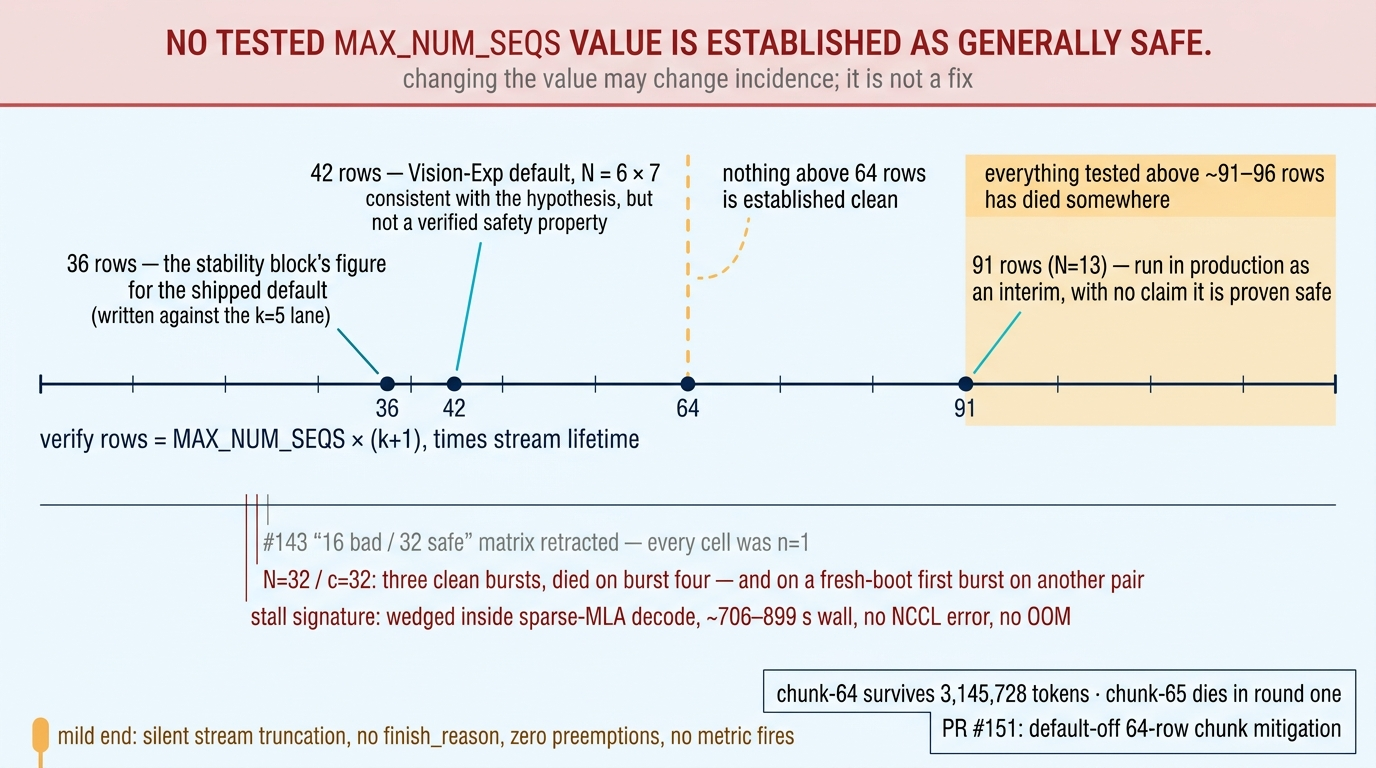
\includegraphics[width=\textwidth]{figures/ch04-verify-rows-141.png}
\caption{The \ghissue{141} evidence on one axis. The best current hypothesis
is geometric --- failure probability rising with verify rows
(\code{MAX_NUM_SEQS} $\times\,(k{+}1)$) times stream lifetime --- but the
evidence is deliberately thin: a retracted $n{=}1$ matrix, stochastic
per-burst stalls, and a production interim its own reporter declines to call
safe. The dashed boundary marks what is not established clean, not a safe
region.}
\label{fig:profile-verifyrows}
\end{figure}

The mild end of the severity spectrum is the dangerous one, because it is
invisible: a short stall cancels the batch, and the result is \emph{silent
stream truncation with no \code{finish_reason}} --- zero preemptions, no
metric fires. \Cref{ch:bugs} follows the full investigation.

\begin{hbwarning}
Two operational rules survive the retraction. No tested
\envvar{MAX_NUM_SEQS} value is established as generally safe under
\ghissue{141}. And if you raise admission, watch for missing
\code{finish_reason} --- it is the earliest signal, well before a watchdog
kill.
\end{hbwarning}

Whatever the profile, concurrent heavy \emph{prefills} remain
scheduler-bound (issues \ghissue{80}/\ghissue{140}): admission tuning raises
decode throughput; it does not fix TTFT contention when several large cold
prompts arrive together.

\section{API authentication}
\label{sec:profile-auth}

Even authentication encodes an incident: the redaction hotfix below is
mandatory and fail-closed because upstream printed keys verbatim. Auth is
optional and enforced by vLLM itself, not a proxy, through two
mutually exclusive variables. \envvar{VLLM_API_KEY} is vLLM's native
single-key env: one bearer key, empty by default (no auth).
\envvar{DSPARK_API_KEYS} is the multi-key form: a single-line,
space/tab-separated list flattened into \emph{one} \code{--api-key} flag ---
the flag is an \code{nargs} list, so repeating it would overwrite rather than
append --- giving each caller an independently revocable key.

If both variables are meaningful, the entrypoint \emph{and} the
start/smoke/status scripts exit 2 naming both, so neither the server nor a
probe ever silently guesses which one applies. Parsing is strict: CR/LF/VT/FF,
backslashes, and any token beginning with \code{-} (which argparse would take
for a vLLM flag) are all rejected with exit 2. The value must live in
\repofile{.env.dspark} --- the launcher sources the file, so an unquoted list
would execute the second key as a command.

Three caveats bound what this auth buys. First, scope: only the prefixes
\code{/v1}, \code{/v2}, and \code{/inference} are guarded. On the pinned
runtime, \code{POST /invocations} and \code{POST /generative_scoring}
\emph{run inference unauthenticated}, and \code{/tokenize},
\code{/detokenize}, \code{/health}, \code{/metrics}, \code{/version}, and
\code{/ping} are likewise keyless --- a keyed deployment still needs
network-level access control on the port (\Cref{fig:profile-apisurface}).

Second, exposure: keys are container argv and environment by design,
readable via host \code{ps} and \code{docker inspect}. Rotation means
editing the line and a full stop/start (no hot reload), and vLLM does not
attribute requests to a key --- this is revocation and blast-radius
control, not per-user logging.

Third, the log channel: upstream's \code{log_non_default_args()} prints
every \code{--api-key} value verbatim at startup. Whenever either variable
is set, the entrypoint therefore requires
\repofile{patches/hotfix-vllm-redact-api-key-log.sh} to apply and verify
(\code{--status}), and fails the container before \code{exec vllm} on any
error --- with no \envvar{DSPARK_SKIP_HOTFIX} bypass. The startup log then
shows \code{'api_key': ['<redacted:N value(s)>']}, preserving the count but
not the bytes.

\begin{figure}[htbp]
\centering
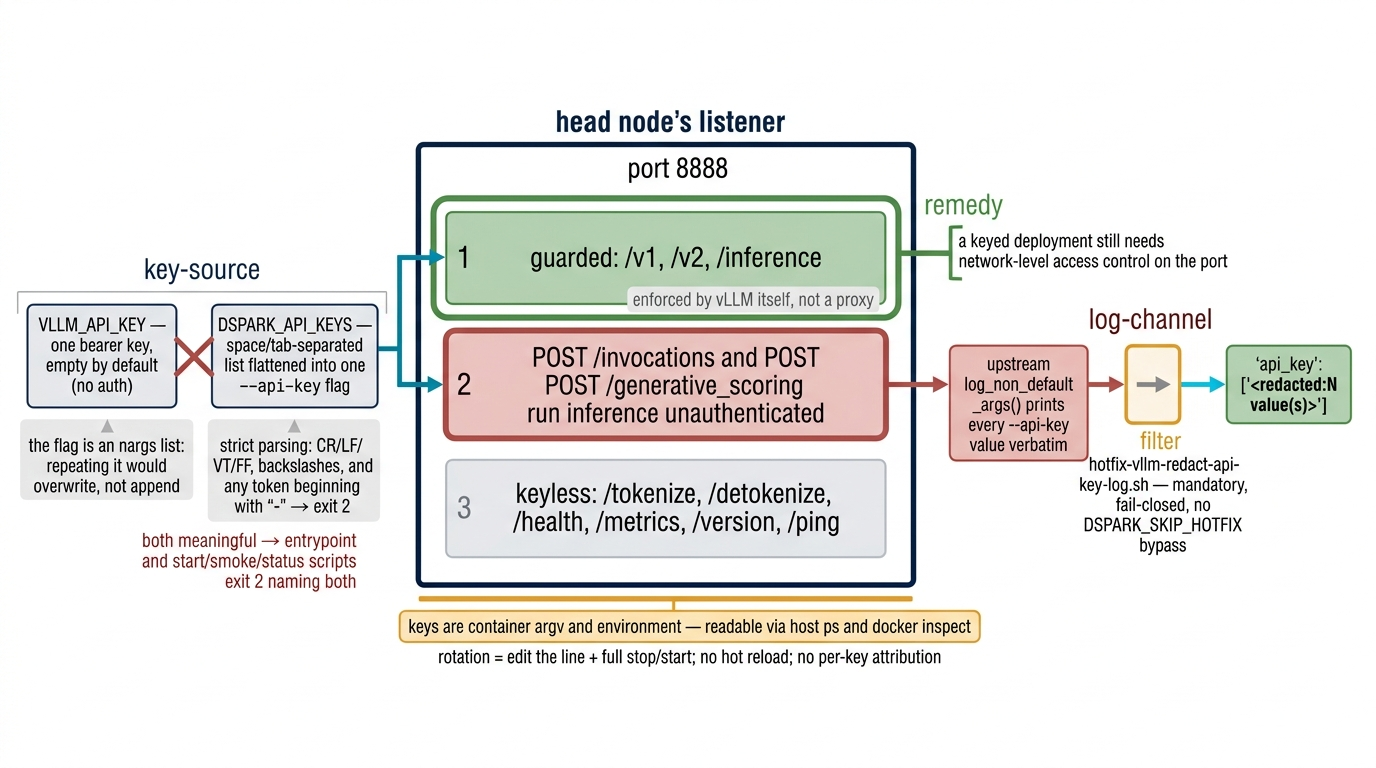
\includegraphics[width=\textwidth]{figures/ch04-api-surface.png}
\caption{What a key buys, and what it does not. vLLM enforces the key on the
\code{/v1}, \code{/v2} and \code{/inference} prefixes only --- two
\code{POST} routes still run inference unauthenticated and six more are
keyless, so network-level access control on the port remains mandatory. The
redaction hotfix is fail-closed with no bypass because upstream prints every
key verbatim at startup.}
\label{fig:profile-apisurface}
\end{figure}

\FloatBarrier
A serving profile stops reading like a list of preferences here. Almost
every value in this argv is either derived from another --- the capture size
from the sequence count and $k$, the utilization from
\envvar{GPU_MEMORY_UTILIZATION_TEXT}, the model from \envvar{ABLITERATED}
--- or the residue of a numbered incident, which is why hand-editing one of
them is how two ranks stop agreeing. And the failures these defaults hold
back are uniformly the quiet kind: a
decode step that silently runs eager, a GID nobody wanted, an answer that
returns null because reasoning spent the budget, a stream that simply stops
with no \code{finish_reason} at all. The flags are the incident log, written
in the only place the engine reads.

\section*{Takeaways}

\begin{itemize}
  \item The serve command is generated, validated, and normalized in stages
    (\repofile{.env.dspark} $\rightarrow$ launcher $\rightarrow$ compose
    $\rightarrow$ entrypoint $\rightarrow$ argv); change knobs at the top and
    never hand-set derived values. \envvar{GPU_MEMORY_UTILIZATION} set by
    hand desynchronizes the ranks, and the CUDA-graph capture size passed
    unrounded --- the arithmetically correct 42 rather than the padded 48
    --- dropped the c=6 step to fully eager at a measured 12\,\% cost
    (122 versus 139~\tokspersec{}). Verify the boot log, not the intention.
  \item Capacity flags are admission ceilings, not reservations: one shared
    pool of 2{,}331{,}430 tokens (17.04\,GiB) is the only thing actually
    spent, the \code{2.22x} boot line answers only the full-1M question, and
    the pool is sized from the minimum across ranks.
  \item \code{max_tokens} counts think plus answer;
    \code{thinking_token_budget} is the precise tool and is doubly opt-in
    (boot flag \ghissue{31} + per-request field), with \ghissue{66} noting a
    decode-cliff risk for omit-field traffic.
  \item To NCCL, defined-empty is not absent: the entrypoint unsets empty
    passthrough keys so config files and per-HCA GID selection are never
    masked --- and on this image a Stage-C-only key is a warn-and-ignore
    no-op, so an unknown-env warning proves nothing either way.
  \item Two things a tuned profile does not buy. Raised admission delivers
    real aggregate throughput (325 \tokspersec{} at c=32), yet no tested
    \code{MAX_NUM_SEQS} is established as generally safe under
    \ghissue{141} --- watch for missing \code{finish_reason}. And an API key
    guards only \code{/v1}, \code{/v2}, and \code{/inference}: two inference
    routes stay open, so network-level access control remains mandatory, as
    does the fail-closed log-redaction hotfix whenever auth is on.
\end{itemize}

\chaptertransition{One rule in this chapter already pointed below the
configuration file. The entrypoint unsets \envvar{NCCL_IB_GID_INDEX}
precisely so that something further down --- NCCL, per HCA --- can make a
choice the profile is not qualified to make, and every number in the profile
assumes that choice comes out right, because both ranks only render the same
argv if the wire between them behaves. That wire carries roughly 108
collectives per decode step and hundreds of megabytes per prefill chunk, and
its arithmetic is uncomfortable the moment you look: each machine advertises
a 200\,Gb QSFP port, and no single PCIe function behind that port can carry
it.}

% =============================================================================
% Chapter 5 — The Fabric: RoCE, NCCL, and the Art of Not Pinning
% =============================================================================
\chapter{The Fabric: RoCE, NCCL, and the Art of Not Pinning}
\label{ch:fabric}

Each DGX Spark in this deployment advertises a 200\,Gb/s QSFP port --- and no
single PCIe function behind that port can carry it. Why that is true, how an
audit proved it, and what it demands of every layer above it is where this
chapter begins (\Cref{sec:fabric-physical}).

The stakes are concrete: every decode step moves roughly 108 NCCL
collectives across the direct QSFP cable between the two machines. Every
prefill chunk pushes hundreds of megabytes of all-reduce traffic over the
same link that also carries the worker's model weights at boot. This chapter
is the fabric layer of the handbook --- how one ConnectX-7 ASIC turns into
four PCIe functions, how NCCL actually parses the device selector you hand
it, why this repository stopped pinning RoCEv2 GID indexes and started validating
them instead, and what evidence a frozen tensor-parallel pair leaves behind
when the forensics were wired in advance. The habits transfer to any
multi-node serving stack, whatever the NIC vendor: verify the PCIe topology
before tuning the network, validate rather than pin, treat defined-empty
environment variables as a distinct hazard, instrument before the incident.

\section{The physical layer: one ASIC, four functions}
\label{sec:fabric-physical}

Each DGX Spark exposes its 200\,Gb/s QSFP networking through a single
ConnectX-7 (CX7) ASIC. The surprise, confirmed during the fable5-1 audit of
2026-09-02 by matching \code{sys_image_guid} across devices, is that this one
ASIC presents \emph{four} PCIe functions to the host: two physical ports, and
\emph{two PCIe functions per port} --- a socket-direct layout. Each physical
function (PF) is wired PCIe Gen5 $\times$4, which is about 15.7\,GB/s
$\approx$ 126\,Gb/s of raw PCIe bandwidth (the launcher's comments call it
``$\sim$100G each'' in practice). The arithmetic is unforgiving: a single PF
cannot carry the port's 200\,Gb/s. Reaching full port rate requires NCCL to
drive \emph{both} PFs of the port at once --- which is exactly what the
dual-HCA configuration in \Cref{sec:fabric-measured} does.

\begin{figure}[htbp]
\centering
\begin{tikzpicture}[font=\small]
  % ---- Spark 1 (head) ----
  \node[hbgpu,minimum width=32mm] (gpu0) {GB10 GPU\\rank 0 (head)};
  \node[hbnode,below=10mm of gpu0.south west,anchor=north west,
        font=\scriptsize] (pf00) {PF f0\\Gen5 $\times$4};
  \node[hbnode,right=3mm of pf00,font=\scriptsize] (pf01) {PF f1\\Gen5 $\times$4};
  \begin{scope}[on background layer]
    \node[hbgroup,fit=(pf00)(pf01),
          label={[hblabel]below:{CX7 ASIC, one QSFP port}}] (cx0) {};
  \end{scope}
  \draw[hbarrow,<->] (gpu0.south) -- (cx0.north);
  % ---- Spark 2 (worker) ----
  \node[hbgpu,minimum width=32mm,right=62mm of gpu0] (gpu1)
        {GB10 GPU\\rank 1 (worker)};
  \node[hbnode,below=10mm of gpu1.south west,anchor=north west,
        font=\scriptsize] (pf10) {PF f0\\Gen5 $\times$4};
  \node[hbnode,right=3mm of pf10,font=\scriptsize] (pf11) {PF f1\\Gen5 $\times$4};
  \begin{scope}[on background layer]
    \node[hbgroup,fit=(pf10)(pf11),
          label={[hblabel]below:{CX7 ASIC, one QSFP port}}] (cx1) {};
  \end{scope}
  \draw[hbarrow,<->] (gpu1.south) -- (cx1.north);
  % ---- RoCE link ----
  \draw[hbflow,<->,very thick] (cx0.east) -- (cx1.west)
    node[midway,above=1mm,align=center,font=\scriptsize,fill=white,
         inner sep=1.5pt]
    {direct QSFP, 200 Gb/s RoCEv2\\NCCL collectives (RDMA)\\
     Gloo/TCPStore bootstrap, ZMQ scheduler (TCP)\\NFS weight reads (TCP)};
  % ---- LAN ----
  \node[hbfaint,below=31mm of gpu0,minimum width=30mm,font=\scriptsize]
        (lan0) {mgmt LAN port};
  \node[hbfaint,below=31mm of gpu1,minimum width=30mm,font=\scriptsize]
        (lan1) {mgmt LAN port};
  \draw[hbarrow,dashed,<->] (lan0.east) -- (lan1.west)
    node[midway,below=6mm,align=center,font=\scriptsize,fill=white,
         inner xsep=4pt,inner ysep=1.5pt]
    {management LAN: SSH orchestration, client API traffic};
  \draw[hbarrow,dashed] (gpu0.west) to[out=180,in=180] (lan0.west);
  \draw[hbarrow,dashed] (gpu1.east) to[out=0,in=0] (lan1.east);
\end{tikzpicture}
\caption{Two-node topology. Each Spark's 200\,Gb/s QSFP port is backed by one
CX7 ASIC exposing two PCIe functions, each Gen5 $\times$4
($\approx$126\,Gb/s), so full port rate needs both PFs. NCCL RDMA, the
Gloo/TCPStore bootstrap, the per-step ZMQ scheduler broadcast, and optional
NFS weight loading all ride the CX7 link (via its IP interfaces); the
launcher's SSH control plane and client API traffic use the management LAN.}
\label{fig:fabric-topology}
\end{figure}

The fable5-1 audit (finding 3, priority P1) inspected both hosts read-only and
found the fabric healthy at the RDMA layer but mistuned at almost every layer
beneath it. \Cref{tab:fabric-health} summarizes the evidence.

\begin{table}[htbp]
\centering\small
\caption{Fabric health snapshot from the fable5-1 audit (2026-09-02, both
nodes, read-only inspection).}
\label{tab:fabric-health}
\begin{tabular}{l>{\raggedright\arraybackslash}p{5.0cm}>{\raggedright\arraybackslash}p{5.2cm}}
\toprule
Observable & Measured & Implication \\
\midrule
RoCE \code{active_mtu} & 1024 (max 4096) & Ethernet MTU 1500 caps IB MTU \\
Ethernet MTU & 1500 (max 9978) & RoCE 4096 needs Ethernet $\geq$ 4200 \\
NIC rings & 1024 (max 8192) & buffer-limited bursts \\
RoCE hw retransmits & 0 & link itself is clean \\
Pause frames & both directions; 1.7\,s tx (head) & global pauses stall NCCL too \\
\code{rx_out_of_buffer} & 13{,}071 (worker) & bursts overflow 1024-slot rings \\
FEC-corrected lane errors & tens of millions & absorbed by RS-FEC; check cable \\
Second-PF subnet & duplicate 10.0.22.0/24 & ARP flux; RTT 0.70 vs.\ 0.33\,ms \\
\bottomrule
\end{tabular}
\end{table}

Three of these deserve unpacking for a reader who has not wired RoCE before.
First, RoCE derives its InfiniBand-side MTU from the Ethernet netdev MTU: with
the stock Ethernet 1500, the RoCE \code{active_mtu} settles at 1024 bytes, and
every RDMA message fragments accordingly. Getting RoCE to its 4096 maximum
requires Ethernet at 4200 or more --- which is why the tuning work in
\Cref{sec:fabric-measured} jumps straight to 9000.

Second, the pause frames
observed here are \emph{global} Ethernet pauses, not priority flow control ---
when the receiver's 1024-entry rings overflow during a burst (the audit
suspected the NFS weight load sharing the link), the pause stalls
\emph{everything} on the wire, NCCL included.

Third, the second PF on each
node carried addresses \code{10.0.22.101}/\code{.102} on the same wire as
\code{10.0.22.1}/\code{.2}. Linux answers ARP for any local address on any
interface, so a duplicate subnet on two interfaces produces textbook ARP flux,
visible as the doubled RTT through the second PF. The audit flagged
de-duplicating that subnet before trusting any dual-PF configuration.

The consequences are asymmetric. Decode collectives are small
($\sim$344\,KB at concurrency 6) and latency-bound, so link bandwidth barely
touches them. Prefill is another story: each 1024-token chunk performs 86
all-reduces of $\sim$8\,MB ($\approx$690\,MB per chunk per rank) plus a
10.9\,MB logits all-gather. At $\sim$11\,GB/s on a single PF that is
$\sim$60\,ms per chunk --- around 15\,\% of a short-context chunk's step time.
This is why the fabric findings promise ``prefill comm bandwidth up to
$\sim$2$\times$; decode $\approx$ unchanged.'' Claiming that 2$\times$,
though, first requires naming the right devices to NCCL --- which is where
the launcher's troubles begin.

\section{Device selection: the NCCL\_IB\_HCA grammar}
\label{sec:fabric-selector}

The launcher must answer a question NCCL never has to: \emph{before}
starting either container, do all the devices this selector will pick
actually have usable RoCEv2 addressing? Answering it requires knowing
exactly what the selector means --- and \envvar{NCCL_IB_HCA} looks like a
device name but is actually a small language. NCCL's \code{parseStringList}
(in \code{src/misc/utils.cc}) accepts an optional leading \code{^} meaning
\emph{exclude the matches}, then an optional \code{=} meaning \emph{exact
name match} instead of the default prefix match, then a comma-separated list
of \code{name[:port[:rail[:plane]]]} tokens. The fine print matters
operationally:

\begin{itemize}
  \item Empty names are dropped, only the first 32 non-empty entries
        (\code{MAX_IB_DEVS}) are stored --- later entries are silently
        ignored --- and each stored name is truncated to the 63-byte payload
        of \code{netIf::prefix} before matching.
  \item An absent \emph{or empty} port field means $-1$, ``any port'':
        \code{devA} and \code{devA:} select exactly the same thing.
  \item A non-empty port field goes through \code{atoi()} --- optional
        whitespace and sign, then leading decimal digits, stopping at the
        first non-digit --- so \code{:08} is decimal port 8 (never octal),
        and \code{:abc} is port 0, which matches no real port.
\end{itemize}

Rail and plane fields are parsed off and ignored for matching here.

Just as important is \emph{what the selector is applied to}. NCCL's
\code{ncclIbInit} builds a candidate universe first: only ports that are
\code{ACTIVE} and whose link layer is Ethernet or InfiniBand, capped again at
32 entries --- and both filters run \emph{before} \envvar{NCCL_IB_HCA} is
consulted. A \code{DOWN} sibling port, common on these dual-port cards, is
simply never a candidate: it cannot fail a match, and NCCL never opens it. A
plain prefix selector like \code{roce} therefore works even on a node where
half the ports are unused. Selection is therefore two filters in series ---
the universe NCCL builds, then the selector the operator writes --- and a
tool that models only the second one will happily validate devices NCCL was
never going to open (\Cref{fig:fabric-hca-selector}).

\subsection{Why the launcher mirrors the grammar byte-for-byte}

To answer the question that opened this section, the start script carries a
shell reimplementation of the selector grammar --- the
\envvar{NCCL_HCA_RESOLVER_BODY} heredoc in
\repofile{start-deepseek-v4-flash-dspark.sh}. The script ships it over SSH
to run \emph{on the node that owns the sysfs tree}, because
\repofile{/sys/class/infiniband} is only meaningful locally. The body is a
quoted heredoc (nothing expands at definition time), and
\code{resolve_rocev2_gid_index} prepends the inputs as \texttt{printf \%q}
assignments so selector tokens travel literally. The resolver runs under
\code{set -f} so a token like \code{roce*} can never glob-expand against the
remote filesystem.

The original version of this resolver, fixed in the 2026-08-20 changelog
entry, used the raw \envvar{NCCL_IB_HCA} value as a sysfs directory name.
Any selector syntax at all --- including the recommended deterministic exact
list \code{=devA,devB} --- produced a path like
\repofile{/sys/class/infiniband/=devA,devB/ports/1/gids} that matched
nothing, and the launcher exited before starting either rank. The rewrite
mirrors NCCL's semantics exactly: \code{^} exclusion, \code{=} exact
matching, the 32-entry cap, the 63-byte name truncation (via a
byte-oriented \texttt{LC\_ALL=C printf '\%.63s'}), and one \code{atoi}-style
conversion per port field.

The subtlest bug in that mirroring is worth a war story.

\begin{hbwarstory}
NCCL's \code{atoi()} happily reads a port number of any width; shell
arithmetic does not. Evaluating an arbitrary-width digit string with
\texttt{\$(( ))} wraps modulo $2^{64}$ --- and one specific input,
\num{18446744073709551615}, wraps to exactly $-1$. In this resolver $-1$ is
not an error value: it is the ``any port'' wildcard. An unrepresentably huge
port field would therefore have silently \emph{widened} the selection to
every port of the device instead of matching nothing. The fix refuses to
evaluate anything wider than a conservative nine digits and clamps it to a
port number no sysfs tree can contain, so the token matches nothing and the
resolve fails closed.
\end{hbwarstory}

The guard in the resolver:

\begin{lstlisting}[language=bash]
if [ -z "$mag" ]; then
  port=0
elif [ ${#mag} -gt 9 ]; then
  # Outside the conservative nine-digit bound. Evaluating arbitrary-width
  # text with $(( )) can wrap the value modulo 2^64 - and
  # 18446744073709551615 wraps to exactly -1, which is the "any port"
  # wildcard - so an unrepresentable port would silently *widen* the
  # selection. Clamp to a value no sysfs port can have: the token then
  # matches nothing and the resolve fails closed.
  port=${sign}999999999
else
  port=$(( 10#$mag ))
  [ -z "$sign" ] || port=$(( 0 - port ))
fi
\end{lstlisting}

The resolver also reproduces the candidate-universe rules: it walks
\repofile{/sys/class/infiniband}, keeps only \code{ACTIVE} ports with an
Ethernet or InfiniBand link layer, treats an \emph{unreadable} attribute as
``still a candidate'' (absence of evidence is not evidence of a down port),
applies the selector, and caps the result at 32, noting on stderr anything
NCCL would ignore. The whole construction is gated by
\repofile{scripts/test-nccl-ib-hca-gid-resolve.sh}, a 72-check suite that
runs the launcher's own generated script against fake sysfs trees ---
covering the 32/33 entry boundary, 63-byte truncation, the leading-zero and
overflow port forms, exclusions, prefix collisions, and DOWN-port handling
--- and fails behaviorally on the pre-fix launcher.

\begin{figure}[htbp]
\centering
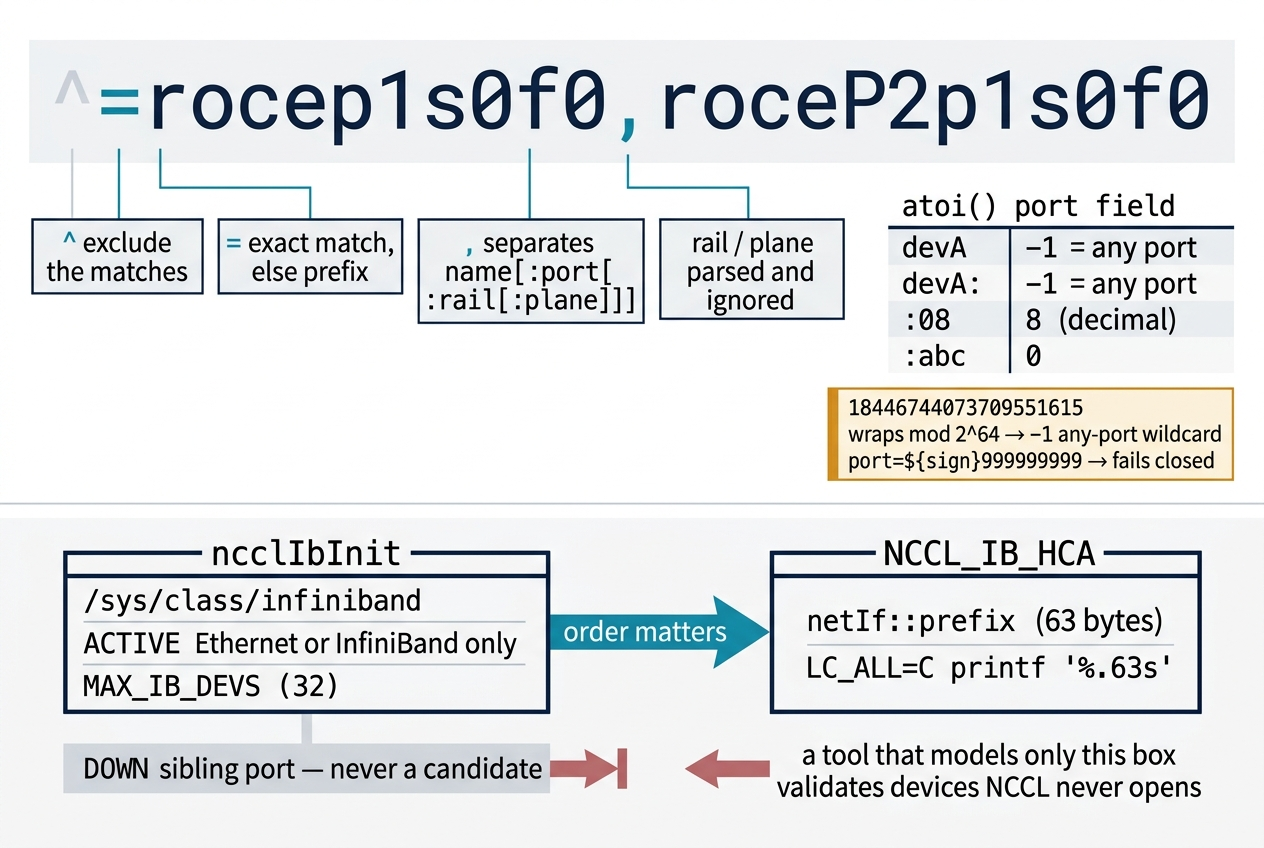
\includegraphics[width=\textwidth]{figures/ch05-hca-selector.png}
\caption{The \envvar{NCCL_IB_HCA} selector is a grammar applied to a universe
NCCL has already built. Top: token anatomy --- optional \code{^} exclusion,
optional \code{=} exact match, comma-separated
\code{name[:port[:rail[:plane]]]} --- with \code{atoi} port semantics, where
\code{devA} and \code{devA:} are both the $-1$ any-port wildcard, \code{:08}
is decimal 8 and \code{:abc} is port 0, and the nine-digit clamp that stops
\num{18446744073709551615} from wrapping to the wildcard. Bottom: selection
is two filters in series. \code{ncclIbInit} keeps only \code{ACTIVE}
Ethernet or InfiniBand ports, capped at 32, before the selector is consulted,
so a \code{DOWN} sibling port can never fail a match --- and a validator that
models only the selector checks devices NCCL was never going to open.}
\label{fig:fabric-hca-selector}
\end{figure}

\section{GID resolution: validate and leave unset}
\label{sec:fabric-gid}

The selector settles \emph{which} ports NCCL drives; addressing settles
whether it can reach anything through them. RoCEv2 identifies an endpoint by
a GID --- for IPv4-based RoCEv2, an
IPv4-mapped address ending in \code{ffff:aabb:ccdd} for \code{a.b.c.d} ---
and each HCA port exposes a small table of them, indexed by integer.
\envvar{NCCL_IB_GID_INDEX} tells NCCL which table entry to use. The trap is
that the usable index is a property of one port on one node at one moment:
it differs per HCA, differs per node, and drifts after reboots, firmware
updates, and link events, because the kernel rebuilds the GID table.

The repository's first answer (PR \ghissue{95} lineage) was to resolve a common
index across all selected members at launch and pin it. The 2026-08-20
resolver even reconciled members by \emph{intersecting} their usable index
sets, exiting with a distinct code when the intersection was empty --- since
\envvar{NCCL_IB_GID_INDEX} is one global value per rank, no single pin can
serve members that disagree. The 2026-09-02 change (credited to tonyd2wild
in issue \ghissue{38}) abandoned pinning entirely, and the reasoning is a
transferable lesson:

\begin{hblesson}
A pin is one global value per rank; the property it pins varies per HCA and
over time. Any pinned index --- including a correctly resolved intersection
--- can later wedge NCCL initialization (\code{ibv_modify_qp} error 61) on a
dual-HCA node after a link event moves the tables. When the underlying
system (NCCL selects the RoCEv2/IPv4 GID \emph{per HCA} whenever the
variable is absent) already does the right thing dynamically, the robust
launcher role is \emph{validation}, not \emph{configuration}: prove at start
time that every selected member has at least one usable GID, print the
evidence, and then leave the variable unset.
\end{hblesson}

Under the default \envvar{NCCL_IB_GID_AUTO}\code{=1}, the resolver therefore
runs in audit mode: for every selected HCA/port it collects \emph{all}
indexes whose GID type is \code{RoCE v2} and whose address matches either
the preferred match IP or an IPv4 on the member's own netdev. (One shared
match IP must not silently disqualify a member living on a different link
address.) Members with disjoint usable sets are fine --- nothing is being
reconciled.

A member with \emph{no} usable RoCEv2 GID is another matter: it aborts the
launch with per-member diagnostics (exit 1, fail closed), before any remote
side effect.

Match IPs come from \code{pick_gid_match_ip}, which prefers an explicit
\envvar{NCCL_IB_GID_MATCH_IP}, then the first IPv4 on the socket interface,
then the configured fabric IP, then the bare worker host address. Stale
\envvar{NCCL_IB_GID_INDEX} pins left in \repofile{.env.dspark} are reported
and ignored, and \envvar{NCCL_IB_GID_AUTO}\code{=0} restores verbatim
pinning for stacks where auto validation is unavailable.

\begin{figure}[htbp]
\centering
\begin{tikzpicture}[font=\small,node distance=5mm]
  \node[hbbox,text width=56mm] (sel) {NCCL\_IB\_HCA selector\\
    \texttt{[\^{}][=]name[:port],...}};
  \node[hbnode,below=of sel,text width=56mm] (parse)
    {Parse (mirrors \texttt{parseStringList}):\\
     32-entry cap, 63-byte names,\\ atoi ports, $2^{64}$-wrap clamp};
  \node[hbnode,below=of parse,text width=56mm] (univ)
    {Candidate universe from sysfs:\\ ACTIVE + Ethernet/InfiniBand\\
     link layer, cap 32 (as \texttt{ncclIbInit})};
  \node[hbnode,below=of univ,text width=56mm] (members)
    {Selected members (per node,\\ run over SSH on the sysfs owner)};
  \node[hbnode,below=of members,text width=56mm] (check)
    {Per member: any RoCE v2 GID\\ matching match-IP or an IPv4\\
     on the member's own netdev?};
  \node[hbwarn,below left=6mm and -22mm of check,text width=30mm]
    (fail) {FATAL, exit 1\\ (fail closed, per-member\\ diagnostics)};
  \node[hbgpu,below right=6mm and -22mm of check,text width=34mm]
    (ok) {Audit usable indexes\\ to stderr; leave\\
    NCCL\_IB\_GID\_INDEX\\ \emph{unset} on both ranks};
  \node[hbfaint,right=10mm of members,text width=26mm,font=\scriptsize]
    (pin) {AUTO=0:\\ pin env values\\ verbatim instead};
  \draw[hbflow] (sel) -- (parse);
  \draw[hbflow] (parse) -- (univ);
  \draw[hbflow] (univ) -- (members);
  \draw[hbflow] (members) -- (check);
  \draw[hbfail] (check.south) -- (fail.north)
    node[hblabel,midway,left=1mm] {none};
  \draw[hbok] (check.south) -- (ok.north)
    node[hblabel,midway,right=1mm] {$\geq 1$};
  \draw[hbarrow,dashed] (pin.west) -- (members.east);
\end{tikzpicture}
\caption{GID auto-resolution under \envvar{NCCL_IB_GID_AUTO}\code{=1}:
selector parse, NCCL-faithful candidate universe, per-member usable-GID
validation, then fail-closed abort or validate-and-leave-unset. NCCL itself
picks the RoCEv2/IPv4 GID per HCA when the index variable is absent.}
\label{fig:fabric-gid-flow}
\end{figure}

\begin{hbwarning}
For NCCL, \emph{empty is not absent}. A defined-but-empty
\envvar{NCCL_IB_GID_INDEX} parses as GID index 0, and because NCCL loads
\repofile{/etc/nccl.conf} (and \envvar{NCCL_CONF_FILE}) with
\code{overwrite=0}, a defined-empty environment variable also \emph{masks}
any config-file value. Compose makes this hazard structural: the compose
file necessarily defines the key. The stack defuses it in two places. The
launcher deliberately keeps emitting \envvar{NCCL_IB_GID_INDEX} --- empty
--- into the worker's SSH environment, so the empty process-level value
out-substitutes a stale pin in the worker's own \repofile{.env.dspark}. The
shared container entrypoint then \emph{unsets} every defined-empty
variable before \code{exec}, so what reaches NCCL is truly absent. Recreate
both ranks (stop then start) after switching modes, or the old in-container
pin survives in the writable layer.
\end{hbwarning}

\begin{figure}[htbp]
\centering
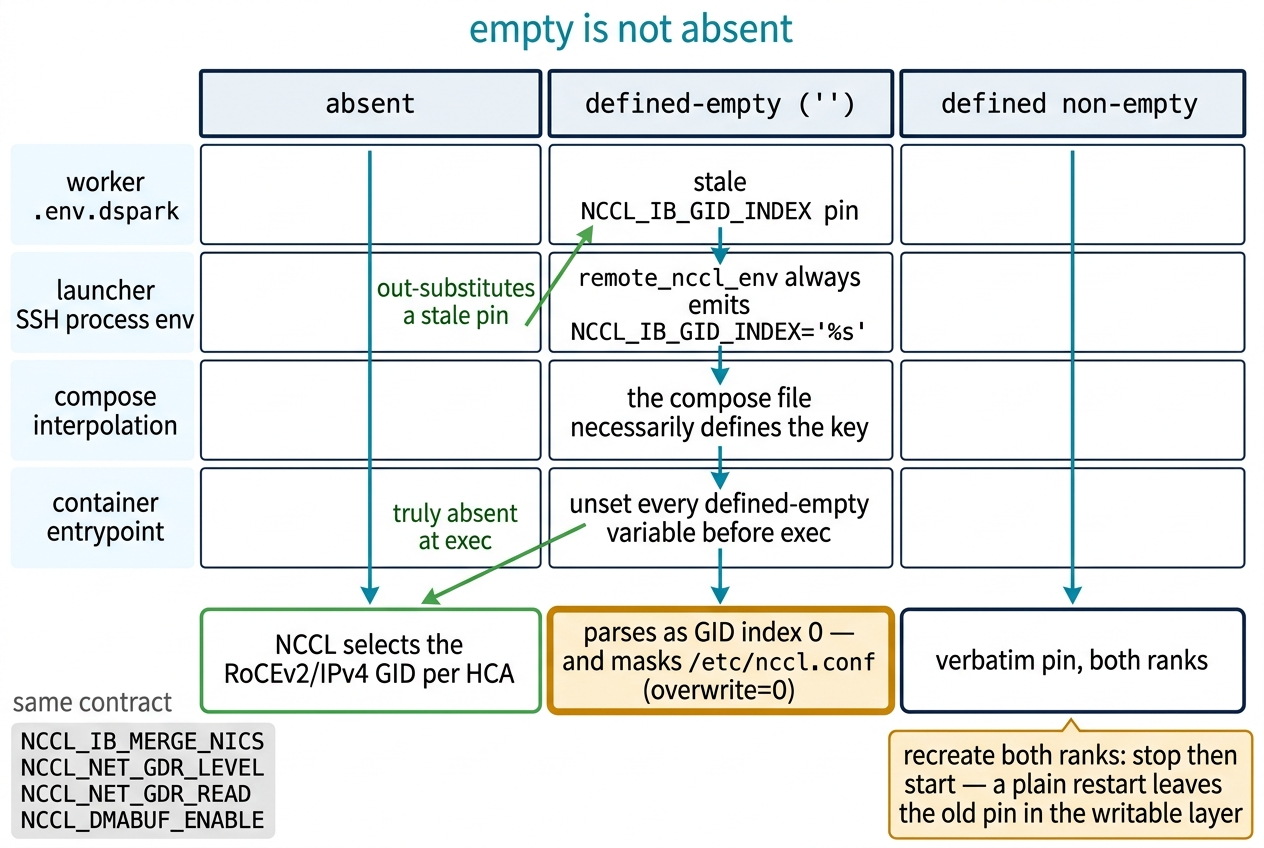
\includegraphics[width=\textwidth]{figures/ch05-empty-not-absent.png}
\caption{Absent, defined-empty, and defined are three different states to
NCCL. A defined-but-empty \envvar{NCCL_IB_GID_INDEX} parses as GID index 0
and, because NCCL loads \repofile{/etc/nccl.conf} with \code{overwrite=0},
also masks the config file --- a hazard Compose makes structural by always
defining the key. The stack defuses it twice: the launcher deliberately emits
the empty value so it out-substitutes a stale pin in the worker's own
\repofile{.env.dspark}, and the shared entrypoint unsets every defined-empty
variable before \code{exec}, so what reaches NCCL is truly absent. The same
contract governs the four fabric passthrough knobs.}
\label{fig:fabric-empty-not-absent}
\end{figure}

\section{Head/worker asymmetry: injecting the worker's view}
\label{sec:fabric-worker}

The warning above leaned on machinery this section owes an explanation: the
launcher deliberately injecting environment into the \emph{worker's} SSH
sessions. The reason is an asymmetry of naming. On a QSFP ring the worker's
port facing the head is often a
differently-named device than the head's port facing the worker, so one
shared \repofile{.env.dspark} cannot describe both nodes. Any mechanism that
feeds both ranks the same values points the worker's NCCL, Gloo, and
scheduler sockets at devices named for the head --- a misconfiguration made
at boot, before any collective can reveal it. The general form is worth
naming, because it recurs wherever a cluster is not symmetric: a setting
whose correct value differs per node cannot live in a file that every node
reads (\Cref{fig:fabric-worker-env}).

The repository's contract: set \envvar{WORKER_NCCL_IB_HCA},
\envvar{WORKER_NCCL_SOCKET_IFNAME}, \envvar{WORKER_TP_SOCKET_IFNAME}, and
\envvar{WORKER_GLOO_SOCKET_IFNAME} in the \emph{head's} env file, and the
launcher injects them into every remote \code{docker compose} invocation as
process environment over SSH. Docker Compose variable substitution is
explicitly ruled out for this job --- a \code{WORKER_*}-first default in the
compose file is not rank-aware, and a shared or scp'd env file would feed
both ranks the same values. Each worker variable defaults to its head
counterpart when unset, so single-name setups need nothing extra. The
injection point is \code{remote_nccl_env}:

\begin{lstlisting}[language=bash]
remote_nccl_env() {
  # Rebuild each call so GID resolve after early init is visible on the
  # worker. NCCL_IB_GID_INDEX is always emitted, even empty under
  # NCCL_IB_GID_AUTO=1: the empty process-env value overrides a stale
  # worker .env.dspark entry at compose interpolation, and the shared
  # entrypoint normalization makes the defined-empty variable truly
  # absent in the container (NCCL would parse a defined-empty value as
  # GID index 0).
  printf "NCCL_IB_HCA='%s' NCCL_SOCKET_IFNAME='%s' TP_SOCKET_IFNAME='%s' \
    GLOO_SOCKET_IFNAME='%s' NCCL_IB_GID_INDEX='%s' ..." \
    "$WORKER_NCCL_IB_HCA" "$WORKER_NCCL_SOCKET_IFNAME" \
    "$WORKER_TP_SOCKET_IFNAME" "$WORKER_GLOO_SOCKET_IFNAME" \
    "$WORKER_NCCL_IB_GID_INDEX"
}
\end{lstlisting}

Two properties of this function are load-bearing. It is rebuilt on every
call, so a GID resolution that happens after early initialization is still
visible to later remote compose commands. And it always emits
\envvar{NCCL_IB_GID_INDEX}, even empty, for exactly the masking reason
described in the hazard box above. The same pattern extends to a third node:
\code{remote_nccl_env2} emits the \envvar{WORKER2_NCCL_*} family for the
optional TP=3 lane (\Cref{ch:scaling}).

\begin{figure}[htbp]
\centering
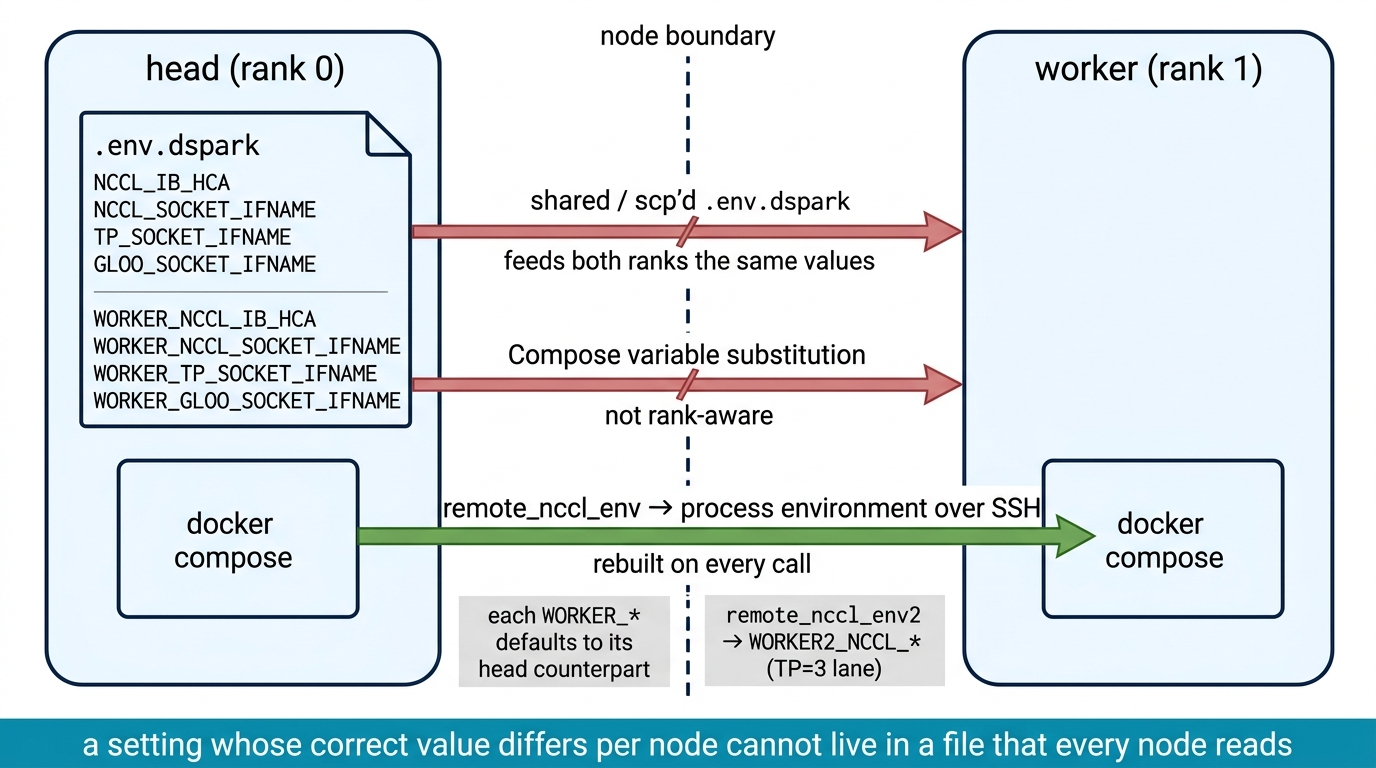
\includegraphics[width=\textwidth]{figures/ch05-worker-env-ssh.png}
\caption{Head/worker asymmetry. The worker's port facing the head is often a
differently named device than the head's port facing the worker, so one
shared \repofile{.env.dspark} cannot describe both nodes. Two plausible
mechanisms are ruled out --- a shared or \code{scp}'d env file and Compose
variable substitution both feed the worker values named for the head --- and
the launcher instead injects the \code{WORKER_*} family as process
environment into every remote \code{docker compose} call, rebuilding it per
call so a GID resolve after early init is still visible. Each
\code{WORKER_*} defaults to its head counterpart, and
\code{remote_nccl_env2} extends the pattern to the optional TP=3 lane.}
\label{fig:fabric-worker-env}
\end{figure}

\section{Measured fabric tuning: dual HCA and MTU 9000}
\label{sec:fabric-measured}

With both ranks guaranteed to address their own devices, the socket-direct
implication of \Cref{sec:fabric-physical} could finally be put to the test.
It was confirmed by measurement on 2026-08-21, on two independent
2$\times$\,GB10 TP=2 pairs with a direct QSFP cable. With only one PF in \envvar{NCCL_IB_HCA}, the link
runs at half the port. The measured configuration listed both controllers
with the deterministic exact-selector form (NIC merging is NCCL's default
behavior) and set MTU 9000 on both controller interfaces at both endpoints:

\begin{lstlisting}[language=bash]
NCCL_IB_HCA==rocep1s0f0,roceP2p1s0f0   # map names: ibdev2netdev
\end{lstlisting}

The results, exactly as the repository records them: pair 1 measured 1311 \tokspersec{}
at MTU 1500 with one HCA, 1343 \tokspersec{} at MTU 9000 with one HCA, and 1410
\tokspersec{} with both HCAs --- \textbf{+7.6\,\%} end-to-end from its own
baseline. Pair 2 reproduced a 1422 \tokspersec{} dual-HCA final rate but has no
same-pair single-HCA baseline, so the repository explicitly declines to quote an
uplift percentage for it --- a small but characteristic act of measurement
hygiene.

Two prerequisites were recorded alongside the numbers. Both interfaces must
be UP with IPs in \emph{distinct} subnets: the duplicate subnet of
\Cref{sec:fabric-physical} had doubled the second PF's round-trip time,
0.70 versus 0.33\,ms, so de-duplicating it is what makes the second PF
worth driving at all. And per-controller PCIe width must be verified
$\times$4 in sysfs (\code{current_link_width}) --- early BIOS revisions wire
the second controller $\times$2. On switched paths, jumbo frames are only safe when
every endpoint and intervening L2 hop is verified at the same MTU.

\begin{hbnote}
Do not transfer microbenchmark deltas to serving throughput. The same
dual-HCA change moved \code{nccl-tests} bus bandwidth by +64\,\% while
end-to-end throughput moved +7.6\,\%: the all-reduce is only a slice of
prefill step time. Engine-counter probes on the measured stack found no
material decode change (code 76.0 \tokspersec{} at 73.3\,\% draft acceptance,
prose 37.3 at 25.7\,\%, 14--15 steps/s) and an unchanged KV pool ---
consistent with decode collectives being latency-bound. The contrast case
is instructive too: an earlier \emph{unmerged} dual-HCA attempt
(2026-08-06), which split channels across two logical NICs instead of
merging both PFs into one, cost KV buffer memory for a +3\,\% result.
\end{hbnote}

Two more findings shape what the defaults do \emph{not} contain. First, no
GPUDirect RDMA was observed on the measured stack: on GB10 driver 580.173.02
the container reported \code{CU_DEVICE_ATTRIBUTE_DMA_BUF_SUPPORTED=0} and
boot logs showed host-staged transport (\code{via NET/IB/x}, no
\code{/GDRDMA}). Every collective therefore bounces through a host buffer,
which on unified memory is an extra GPU-side memcpy rather than a PCIe hop.
The repository is careful to scope this as a contributor-reported observation on
that stack only, not a claim about GDR in general.

Second, the four NCCL passthrough
knobs (\Cref{tab:fabric-passthrough}) all default to \emph{unset}, with a
precise absence contract. Compose necessarily defines each key, but the
entrypoint unsets empty definitions before \code{exec}, so NCCL's built-in
defaults and config-file values still apply and cannot be masked by a
defined-empty value. Configured non-empty values pass through unchanged on
both ranks (\Cref{fig:fabric-empty-not-absent}).

\begin{table}[htbp]
\centering\small
\caption{NCCL fabric passthrough knobs (all default unset; empty is
normalized to absent by the entrypoint).}
\label{tab:fabric-passthrough}
\begin{tabular}{lp{86mm}}
\toprule
Variable & Role \\
\midrule
\envvar{NCCL_IB_MERGE_NICS} & NCCL default is 1: \emph{permits} merging
compatible dual-port NICs into one logical device; it selects nothing and
forces nothing. The meaningful override is 0, to disable merging. \\
\envvar{NCCL_NET_GDR_LEVEL} & Upstream GPUDirect override; no effect
demonstrated on the submitted GB10 stack. \\
\envvar{NCCL_NET_GDR_READ} & Upstream GPUDirect override; same status. \\
\envvar{NCCL_DMABUF_ENABLE} & 0 disables DMA-BUF probing --- the meaningful
workaround control where probing misbehaves. \\
\bottomrule
\end{tabular}
\end{table}

Taken together, the tuning surface here is narrower than it looks. Two PFs
and MTU 9000 are the measured win; everything else in
\Cref{tab:fabric-passthrough} ships unset because nothing on this stack
demonstrated a reason to set it.

\section{Forensics: the flight recorder and the FIFO poke}
\label{sec:fabric-forensics}

A tuned and validated fabric can still freeze mid-collective --- and when it
does, what matters is the evidence it leaves behind. The mechanism below has
two halves, and both must be in place long before they are needed: a
recorder that runs on every boot, and a trigger an external watchdog can
pull on a rank that is frozen but has not yet timed out. Every tensor-parallel
pair loss in this deployment's history (the issue
\ghissue{117} class, and the stochastic \ghissue{141} stalls of
\Cref{ch:bugs}) ended the same way: the stalled rank logged nothing, and the
peer spun in a collective until torch's ProcessGroupNCCL watchdog killed it
at 600\,s. After the restart only coarse metrics remained --- zero
collective-level evidence. The issue \ghissue{117} disposition wired
PyTorch's flight recorder permanently into the compose environment:

\begin{lstlisting}
TORCH_FR_BUFFER_SIZE=2000
TORCH_NCCL_DUMP_ON_TIMEOUT=1
TORCH_NCCL_ENABLE_MONITORING=1
TORCH_FR_DUMP_TEMP_FILE=/cache/huggingface/nccl-fr/comm_lib_trace_rank_
TORCH_NCCL_DEBUG_INFO_PIPE_FILE=/tmp/fr_dump_pipe_
\end{lstlisting}

The three switches are pinned together deliberately: the torch header
documents that dump-on-timeout requires monitoring enabled \emph{and} a
nonzero ring-buffer size, so even though 2000/1/1 match torch 2.11 defaults,
all three are set explicitly. Dumps land on the persistent Hugging Face
cache volume, so a watchdog-killed pair still leaves per-rank evidence for
\code{torchfrtrace} --- which aligns both ranks' ring buffers to distinguish
a collective desynchronization from a rank that stalled before enqueuing its
next collective.

The pipe stem is the on-demand trigger, and its placement encodes a boot
constraint: torch \code{TORCH_CHECK}s the \code{mkfifo} at process-group
init, so the stem must never point into a directory that might not exist
(an unmounted volume path would fail the boot). Hence \repofile{/tmp} ---
which in this stack is \emph{not} container-local. It is the
\envvar{DSPARK_TMP_HOST} bind mount (host default
\repofile{~/.cache/dspark-tmp}), so the FIFO is host-visible there and
root-owned; host-side pokes need root, or use \code{docker exec}, and torch
unlinks and recreates a stale FIFO from a previous container. Writing
anything to \repofile{/tmp/fr_dump_pipe_<rank>.pipe} inside the container
requests an on-demand dump --- the hook an external watchdog uses to capture
evidence from a rank that is frozen but has not yet timed out.

\begin{figure}[htbp]
\centering
\begin{tikzpicture}[font=\small,node distance=4.5mm]
  \node[hbwarn,text width=98mm] (hang)
    {\textbf{t0} --- rank frozen mid-collective (peer spinning; torch 600\,s
     watchdog not yet fired)};
  \node[hbnode,below=of hang,text width=98mm] (poke)
    {\textbf{t1} --- watchdog script pokes the FIFO: write anything to
     \texttt{/tmp/fr\_dump\_pipe\_$<$rank$>$.pipe} (root or
     \texttt{docker exec})};
  \node[hbnode,below=of poke,text width=98mm] (wait)
    {\textbf{t2} --- torch dumps \emph{asynchronously} (\texttt{std::async},
     best-effort): wait for ``Finished writing Flight Recorder debug
     info'' in the log, or for the dump file size to settle};
  \node[hbnode,below=of wait,text width=98mm] (archive)
    {\textbf{t3} --- archive \texttt{comm\_lib\_trace\_rank\_*} from
     \emph{both} nodes together into one directory (filenames are static
     per rank; the next dump truncates them)};
  \node[hbgpu,below=of archive,text width=98mm] (restart)
    {\textbf{t4} --- only now restart the pair; run \texttt{torchfrtrace}
     offline over the complete rank set};
  \draw[hbflow] (hang) -- (poke);
  \draw[hbflow] (poke) -- (wait);
  \draw[hbflow] (wait) -- (archive);
  \draw[hbflow] (archive) -- (restart);
\end{tikzpicture}
\caption{Flight-recorder incident response for a frozen-but-not-timed-out
rank. Restarting before t2 completes can kill the writer mid-dump;
archiving one rank alone leaves \code{torchfrtrace} without the rank set it
needs. A watchdog timeout at 600\,s triggers t2 automatically.}
\label{fig:fabric-fr-timeline}
\end{figure}

Two operator rules are part of the documented contract, and both exist
because someone can otherwise destroy the evidence they just captured.
First, dump filenames are static per rank and torch \emph{truncates on every
dump}. Archive both ranks' \repofile{comm_lib_trace_rank_*} together
after each dump, before the next poke or timeout overwrites them ---
\code{torchfrtrace} needs the complete rank set in one directory, and each
node's volume holds only its own rank's file. Second, a poke only
\emph{requests} a dump: torch launches the write via \code{std::async} and
never waits, so an immediate restart can kill the writer mid-dump and leave
a truncated or missing file. Wait for the ``Finished writing Flight
Recorder debug info'' log line or a bounded file-size-settle check before
touching the pair.

The 200\,Gb/s printed on the QSFP port was never a property of the cable.
It is a claim about PCIe width, Ethernet MTU, ring depth, subnet layout and
device naming --- each of which can quietly halve it, and none of which
announces itself in a collective that merely runs slowly. What changed along
with that picture is the launcher's job on the fabric: it stopped
\emph{configuring} the network and started \emph{proving} it, because a pin
is one global value per rank while the property being pinned varies per HCA
and moves after every link event. The strongest fabric work in this chapter
is not a tuning value at all; it is a validator that refuses to boot, and a
recorder that was already running when the pair froze.

\FloatBarrier
\section*{Takeaways}
\begin{itemize}
  \item Know your PCIe topology before tuning the network: full port rate
        needs both Gen5 $\times$4 PFs in \envvar{NCCL_IB_HCA} with
        \code{current_link_width} verified $\times$4, and RoCE inherits its
        MTU from Ethernet --- netdev 1500 caps \code{active_mtu} at 1024, so
        the measured recipe is MTU 9000 at both endpoints with distinct
        subnets per PF.
  \item \envvar{NCCL_IB_HCA} is a grammar applied to a pre-built candidate
        universe of ACTIVE ports --- mirror it exactly or validate devices
        NCCL was never going to open. Mirror the arithmetic too: shell
        \texttt{\$(( ))} wraps modulo $2^{64}$ and $2^{64}{-}1$ wraps to the
        any-port wildcard $-1$, so clamp unrepresentable ports and let bad
        input narrow the selection instead of widening it.
  \item Validate, don't pin: GID indexes drift per HCA and over time, so
        prove a usable GID per member, fail closed otherwise, and leave the
        index unset --- remembering that defined-empty is not absent to
        NCCL, since an empty \envvar{NCCL_IB_GID_INDEX} parses as index 0
        and masks \repofile{/etc/nccl.conf}, which is why the entrypoint
        unsets defined-empty variables before \code{exec}.
  \item Microbenchmarks do not transfer: +64\,\% \code{nccl-tests} bus
        bandwidth became +7.6\,\% end-to-end, and pair 2's number ships
        without an uplift claim for want of a same-pair baseline.
  \item Wire forensics before the incident: flight recorder pinned on,
        dumps on a persistent volume, a FIFO poke for frozen ranks ---
        archive both ranks together and never restart mid-dump.
\end{itemize}

\chaptertransition{Everything validated here stops at the container door. The
launcher can prove that both ranks address their own HCAs and still hand them
a pinned third-party image whose serving code needs roughly forty corrections
before it is fit to run this model --- so the same fail-closed reasoning has
to go inside, rewriting the installed engine at every boot without ever
letting unverified code serve a request. The next chapter is that method, and
it opens where the method once failed: a boot sequence whose patchers were
separated by bare semicolons, so a missing file or a drifted anchor was
swallowed by the next successful command and the server came up looking
perfectly healthy on stale code.}

% =============================================================================
% Chapter 6 — The Patch Train: Fail-Closed Runtime Surgery
% Sources: book-notes/patches-digest.md, book-notes/scripts-digest.md,
%          repo docker-compose.dspark.yml (entrypoint), CHANGELOG.md,
%          docs/PATCHES.md
% =============================================================================

\chapter{The Patch Train: Fail-Closed Runtime Surgery}
\label{ch:patches}

Until the 2026-08-22 fail-closed conversion (issue \ghissue{107}), this
deployment's boot sequence contained a quiet trap: its default-on Python
patchers were separated by \emph{bare semicolons} in the container
entrypoint, so a missing patch file, an anchor drift, or a failed self-check
was masked by the next successful command. The server started anyway,
serving stale runtime code with every appearance of a clean boot. The
principle the fix encoded is the thesis of this chapter: \emph{an enabled
boot must never silently serve stock behavior.}

The trap existed because of a question every inference deployment that pins a
third-party runtime image eventually faces: the image has bugs, upstream has
fixes (or you have written your own), and the model must keep serving. This
repository's answer is a corpus of more than forty patch files that rewrite
the installed vLLM tree \emph{inside the container, at every boot, before}
\code{exec vllm serve} --- a ``patch train'' that either delivers a
byte-verified runtime or refuses to start at all. This chapter is about the
method, not the individual bugs (those are the subject of \Cref{ch:bugs}):
how the patchers are structured, how they are gated, how independent fixes
compose on the same files, and how a CPU-only CI gate keeps the whole
apparatus honest.

For an inference engineer, this is the most transferable material in the book
--- any team running a pinned engine image on hardware upstream does not test
will end up building something like it. This repository shows what the mature
form looks like: fail-closed gating, byte-exact provenance, and rollback by
recreation rather than by hope.

\section{The strategic choice: patch a pinned image at boot}
\label{sec:patches-strategy}

The deployment target throughout is one image, pinned by registry manifest
digest:

\begin{lstlisting}
ghcr.io/anemll/dspark-vllm-gx10:0.1.1
  @sha256:a83948492cf13df455170fb42885f5ef4db54fefe0feff0f841ecbff464ac9d8
  -> config/image ID sha256:3430d6614a8e2925f34d059af6caf05aff42387326db4d05639a60f10f2654d8
carrying vLLM 0.25.2.dev0+g752a3a504.d20260714
installed at /usr/local/lib/python3.12/dist-packages/vllm
\end{lstlisting}

The obvious alternative --- fork the image, apply the fixes at build time, and
ship a rebuilt image --- was rejected. Patch-at-boot buys three things the
fork cannot easily provide:

\begin{itemize}
\item \textbf{Byte-exact provenance.} The runtime tree at any moment is a pure
  function of two published artifacts: the pinned digest and the patch corpus.
  Several patchers make this literal, pinning the SHA-256 of the file they
  expect to find and of the file they leave behind, so ``what code is this
  rank actually running?'' has a checkable answer.
\item \textbf{Tiny, reviewable diffs.} Each fix is one file with its own
  docstring, evidence, marker, and \code{--status} mode --- not a commit
  buried in an image rebuild. The whole train is legible in the compose
  entrypoint.
\item \textbf{Rollback by recreation.} Because patches live only in the
  container's writable layer, discarding the container (\code{docker rm} and
  a fresh \code{create}) restores the pristine pinned image exactly. Turning
  a fix off is a flag flip plus a recreate --- no image rebuild, no registry
  round-trip.
\end{itemize}

The costs are real and the repository documents them bluntly. Patched bytes live in
the writable layer, so the layer becomes hidden state: a plain
\code{docker restart} \emph{keeps} whatever the previous boot wrote.
\repofile{docs/PATCHES.md} states the doctrine for the \ghissue{136}
patcher in one sentence: ``\code{docker restart} or restarting the process
reuses the patched writable layer and is \textbf{not} rollback.'' Every
flag change therefore requires a paired stop/remove/start on both nodes.
The patchers themselves must be engineered to meet a tree that some earlier
boot already modified --- which is why idempotence, drift detection, and
multi-pre-image pinning (\Cref{sec:patches-compose}) are first-class problems
here rather than afterthoughts (\Cref{fig:patch-writable-layer}).

\begin{hbwarstory}
The TP=3 patcher learned the writable-layer lesson ``the hard way.'' Its
idempotence markers were originally derived from each edit's description
alone, so when a patch \emph{body} changed, a container whose writable layer
held the \emph{old} body still looked ``already patched.'' The stale
code survived every compose restart, with the only symptom a shape assert on
rank 2. The fix: markers now embed a SHA-256 prefix of the replacement body.
A stale body yields a \code{STALE} verdict, which is a hard exit-1 failure
with explicit remediation --- \code{docker rm -f} on every node, because the
anchor has been consumed and the file cannot be re-anchored in place.
\end{hbwarstory}

\begin{figure}[htbp]
\centering
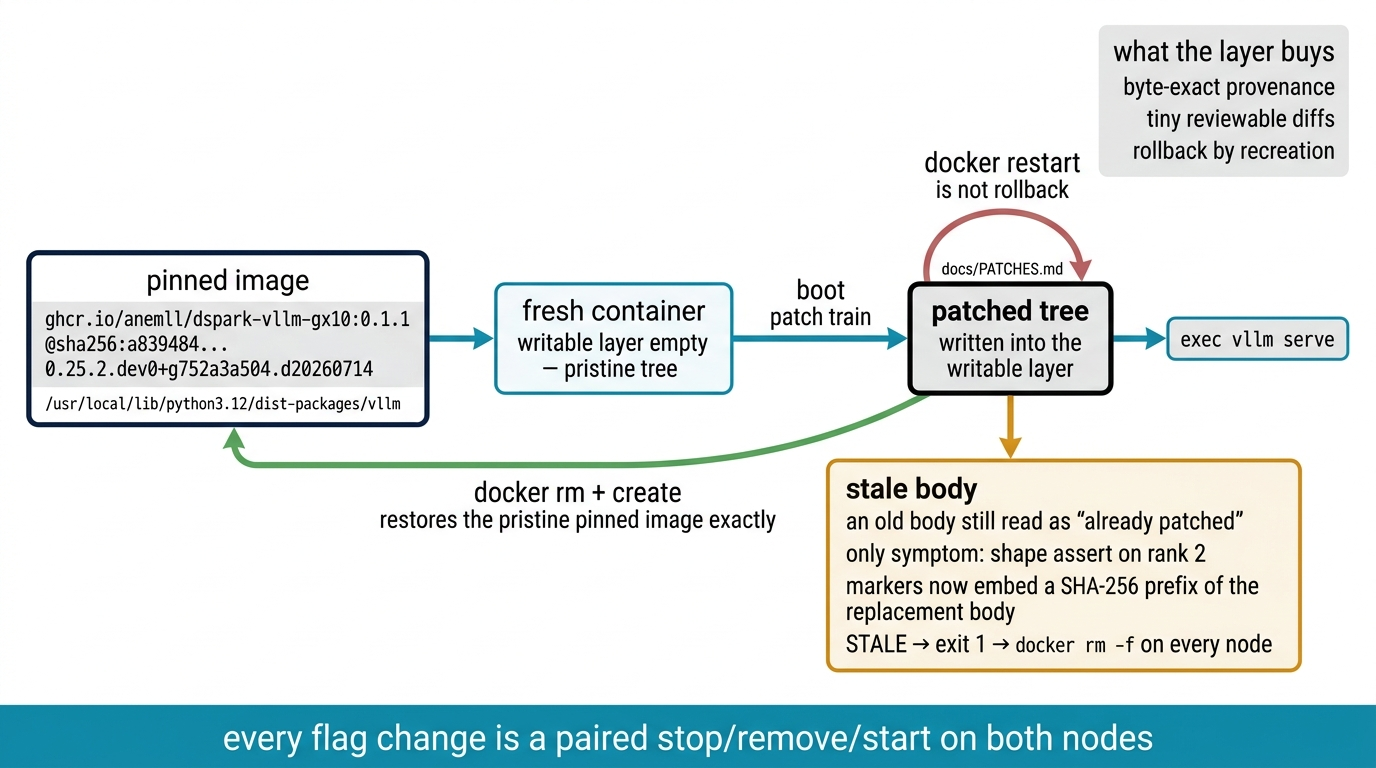
\includegraphics[width=\textwidth]{figures/ch06-restart-not-rollback.png}
\caption{Patched bytes live only in the container's writable layer. That is
what makes rollback a recreate rather than an image rebuild --- but it also
makes the layer hidden state: \code{docker restart} reuses whatever the
previous boot wrote and is not rollback, so every flag change is a paired
stop/remove/start on both nodes. The TP=3 patcher learned the corollary the
hard way: idempotence markers derived from an edit's description alone let a
stale body still read as ``already patched'', surviving every compose restart
with a shape assert on rank 2 as the only symptom. Markers now embed a
SHA-256 prefix of the replacement body, and a stale body is a hard
\code{STALE} exit 1 demanding \code{docker rm -f} on every node.}
\label{fig:patch-writable-layer}
\end{figure}

\section{Four patcher families}
\label{sec:patches-families}

The corpus that grew up under these constraints --- idempotence against a
dirty writable layer, drift detection, stale-body refusal --- is not
uniform: it shows an escalating ladder of verification rigor matched to
blast radius. \Cref{tab:patch-families} summarizes the four
recognizable families; the subsections that follow give one worked example of
each.

\begin{table}[htbp]
\centering
\small
\caption{The four patcher families, ordered by verification rigor.}
\label{tab:patch-families}
\begin{tabular}{>{\raggedright\arraybackslash}p{3.4cm}>{\raggedright\arraybackslash}p{4.3cm}>{\raggedright\arraybackslash}p{3.2cm}>{\raggedright\arraybackslash}p{3.2cm}}
\toprule
Family & Integrity mechanism & Failure handling & Examples \\
\midrule
Anchor+marker Python startup patchers & exact-anchor match, occurrence
  counts, \code{compile()} before write, marker comment & exit 1 on
  anchor drift; idempotent re-runs & \ghissue{27}, \ghissue{43},
  \ghissue{26} v2, \ghissue{133}, adaptive chunk \\
Transactional multi-hunk shell backports & staged in-memory view; all hunks
  validate before any write; atomic per-file rename & post-commit byte
  verify; reverse-order rollback of published files & upstream PRs
  \ghissue{48407}, \ghissue{48957}, \ghissue{49486}, \ghissue{50298},
  \ghissue{50312}, \ghissue{44993} \\
SHA-256 pre/post-image patchers & whole-file or AST-extracted-method hash
  pins; version pins; TOCTOU stat guards & staged rollback image; verified
  restore; loud exit 2 if restore fails & \ghissue{117}, \ghissue{136}/210,
  \ghissue{138}, codex, \ghissue{141}, block-k, responses store \\
Overlay packages and reference patches & normal Python import (via an
  appended hook) or plain unified diff & fail-closed installer; diffs
  are documentation or build-time & \repofile{vision_exp/}, \repofile{tp3/},
  three \code{.patch}/\code{.diff} files \\
\bottomrule
\end{tabular}
\end{table}

\subsection{Anchor+marker startup patchers}

The workhorse family: idempotent Python scripts that match \emph{exact stock
source text}, replace it once, syntax-check the result, and write back. The
shape, common to a dozen scripts, is:

\needspace{12\baselineskip}
\begin{lstlisting}[language=Python]
# representative shape (pseudocode distilled from the family)
src = target.read_text()
if MARKER in src:            # idempotent: an earlier boot already patched
    verify_and_exit(0)
assert src.count(OLD) == 1   # anchor drift or ambiguity -> SystemExit(1)
patched = src.replace(OLD, NEW_WITH_MARKER, 1)
compile(patched, str(target), "exec")   # syntax gate BEFORE any write
target.write_text(patched)
# every script also answers --status: APPLIED / NOT APPLIED / stale states
\end{lstlisting}

A representative member is
\repofile{patches/hotfix-dsv4-adaptive-prefill-chunk.py} (67 lines): it
anchors the two chunk-cap sites in the v1 scheduler, asserts both anchors are
present, widens the cap logic so a cold single-request prefill is not chunked,
compiles before writing, and tags its work with the marker comment
\code{[dspark-adaptive-chunk]}.

The family also supports \emph{revisioned}
patches: the \ghissue{27} scheduler patcher carries r3 markers and
refuses with exit 1 if it finds an older r2 application, because the r2
anchors were consumed and only a pristine file can be re-patched. It reports
\code{APPLIED (r2, stale)} rather than guessing. The most interesting member,
the \ghissue{26} hotfix, is a patcher that \emph{reverts its own v1}:
its \code{apply_text()} recognizes three file states (stock, v1-injected,
already-v2) and replaces an in-image v1 injection with the corrected v2
block, since v1 had caused warm-prefix garbage (\Cref{ch:bugs}).

\subsection{Transactional multi-hunk shell backports}

The upstream-PR backports (\ghissue{48407}, \ghissue{48957}, \ghissue{49486},
\ghissue{50298}, \ghissue{50312}, \ghissue{44993}) each change several hunks
across one to four files, and a partially applied backport would be worse than
none. The family's answer is to take the database vocabulary literally: a
backport is a transaction over files, and atomic per-file rename is enough
primitive to build one. Each is a bash wrapper around an embedded Python ``whole-script
transaction'': every hunk validates against an in-memory staged view of its
target, and nothing touches disk until \emph{all} hunks validate and compile.
Publication is per-file atomic (\code{mkstemp} in the same directory,
\code{fsync}, \code{os.replace}, directory \code{fsync}), and the committed
bytes are re-read and verified. Any failure rolls back every
already-published file in reverse order --- with a nonzero, loud exit if the
rollback itself fails. Per-hunk state is a
\code{count(old)}/\code{count(new)} machine: $(1,0)$ applies, $(0,1)$ is
already patched, anything else is refused as ambiguous. A
\code{_track_published} guard even covers the race where an interrupt lands
after the rename syscall but before bookkeeping. \Cref{fig:patch-transaction}
draws the state machine.

The worked example is
\repofile{patches/hotfix-dsv4-flashmla-workspace-50298.sh} (542 lines,
six hunks across two files): it backports upstream vLLM PR \ghissue{50298},
which removed a per-chunk \code{torch.full(-1)} allocation on the sparse
prefill path by reserving the two int32 index buffers in the capture-time
workspace and threading an \code{out=} parameter through
\code{combine_topk_swa_indices()}. Six edits, two files, one transaction:
either both files end up in the post-image state, or neither does.

\begin{figure}[htbp]
\centering
\begin{tikzpicture}[node distance=4.5mm and 8mm]
  % idempotent shortcut (left column)
  \node[hbfaint, text width=2.9cm] (idem)
    {already patched:\\ \scriptsize re-verify only,\\ \scriptsize no write};
  % main pipeline (center column)
  \node[hbnode, text width=4.4cm, right=16mm of idem] (val)
    {\textbf{1.\ validate pre-image}\\ \scriptsize SHA-256 / anchor-count state
     machine over a staged in-memory view; ambiguity refused};
  \node[hbnode, text width=4.4cm, below=of val] (build)
    {\textbf{2.\ build + compile}\\ \scriptsize all candidate files constructed
     and syntax-checked in memory; nothing written yet};
  \node[hbnode, text width=4.4cm, below=of build] (stage)
    {\textbf{3.\ stage}\\ \scriptsize same-directory temp file,
     mode preserved, fsync};
  \node[hbbox, text width=4.4cm, below=of stage] (rename)
    {\textbf{4.\ publish}\\ \scriptsize atomic os.replace + directory fsync,
     file by file in order};
  \node[hbnode, text width=4.4cm, below=of rename] (verify)
    {\textbf{5.\ re-verify}\\ \scriptsize re-read published bytes:
     hash, mode, compile};
  \node[hbgpu, text width=4.4cm, below=of verify] (ok)
    {\textbf{committed} --- exit 0};
  % rollback column (right)
  \node[hbwarn, text width=3.6cm, right=of rename] (rb)
    {\textbf{rollback}\\ \scriptsize restore every published file in
     \emph{reverse} order from staged rollback images};
  \node[hbwarn, text width=3.6cm, below=of rb] (rbver)
    {restore verified\\ \scriptsize exit 1 --- boot blocked};
  \node[hbwarn, text width=3.6cm, below=of rbver] (fatal)
    {rollback failed\\ \scriptsize loud FATAL --- exit 2};
  % flows
  \draw[hbflow] (val) -- (build);
  \draw[hbflow] (build) -- (stage);
  \draw[hbflow] (stage) -- (rename);
  \draw[hbflow] (rename) -- (verify);
  \draw[hbok]   (verify) -- (ok);
  \draw[hbarrow] (val) -- node[hblabel, above, font=\tiny]{post-image} (idem);
  \draw[hbok]   (idem.west) -- ++(-5mm,0) |- (ok.west);
  \draw[hbfail] (rename.east) -- node[hblabel, pos=0.4, above=0.5mm,
    font=\tiny, fill=white, inner sep=1pt]{publish fails} (rb.west);
  \draw[hbfail] (verify.east) -- (rb.south west);
  \draw[hbfail] (rb) -- (rbver);
  \draw[hbfail] (rbver) -- node[hblabel, right]{restore mismatch} (fatal);
  \node[hblabel, text width=2.6cm, align=center, below=4mm of idem] (drift)
    {drift / ambiguity:\\ exit 1, no write};
  \draw[hbfail] (val.south west) to[bend right=15] (drift.north);
\end{tikzpicture}
\caption{The transactional patcher state machine shared by the multi-hunk
backports and the SHA-pinned family. Failures in steps 1--2 exit before any
write; failures at publish or verification trigger a verified reverse-order
restore of everything already published. An already-patched target takes the
idempotent path: re-verify, never rewrite.}
\label{fig:patch-transaction}
\end{figure}

\subsection{SHA-256 pre/post-image patchers}

The strictest family locks the \emph{complete file} (or a complete
AST-extracted method) by SHA-256 pre-image and post-image, refuses any drift,
stages a rollback image before touching the target, and verifies bytes, mode,
and source state after publication. The bounded Responses-store patcher is the
canonical whole-file example. Its contract, published verbatim in
\repofile{docs/PATCHES.md}:

\needspace{6\baselineskip}
\begin{lstlisting}
/usr/local/lib/python3.12/dist-packages/vllm/entrypoints/openai/responses/serving.py
stock SHA-256   fe3a48ab09c516835ce6dd1471c06cc784ae7504eaa7af7f10574704106830d8
patched SHA-256 1b0033131a34e03a2e129743258f5da81b3e60e979072920153f6d09bf4e5d8f
\end{lstlisting}

Fourteen named anchor$\rightarrow$replacement pairs are applied in order, and
the result must hash to the pinned post-image before an atomic publish. The
transform turns vLLM's self-described leak (``may cause a memory leak since we
never remove responses from the store'') into an LRU-bounded store capped by
\envvar{DSPARK_RESPONSES_STORE_MAX_ENTRIES} (default 256). The extreme of
whole-file pinning is the \ghissue{117} patcher: four pinned
whole-file identities, a TOCTOU guard that \code{lstat}s the target before
and after reading it, a rename-race probe, and a rollback that re-verifies
bytes, metadata, state, and compilation.

The \ghissue{138} and codex patchers refine the granularity: rather
than pinning a whole file that other patches may legitimately touch, they use
\code{ast.parse} to extract the one \code{input_item_parsing} method from
\repofile{entrypoints/openai/responses/protocol.py}, require the extracted
text to occur exactly once, and pin \emph{that method's} SHA-256 (old
\code{2412484a...}, expected new \code{536f3a30...}) plus two ordered
outer guards --- a method-granular source lock that survives changes elsewhere
in the file.

Several members also pin the environment itself: the block-k patcher
requires the installed vLLM version string to equal
\code{0.25.2.dev0+g752a3a504.d20260714} via \code{importlib.metadata}, and
the \ghissue{136} chain pins the \code{xgrammar} version (0.2.3) as
well.

The \ghissue{141} workaround pushes pinning across a package
boundary. Its correctness argument rests on the pinned FlashInfer revision's
dispatch contract --- calls of at most 64 rows take the standalone DSv4
decode kernel. The patcher therefore pins exact guard fragments from FlashInfer
itself: the 64-row cutoff in the workspace helper, the
\code{_DECODE_MAX_TOKENS = 64} definition, the dispatch predicate, the
adapter call signature, and the custom-op \code{mutates_args} contract that
excludes both KV caches. Each fragment must occur exactly once \emph{and in
pinned relative order} --- the check verifies offset monotonicity, so even
guard \emph{reordering} counts as drift. The patcher thereby verifies not
just the code it rewrites but the code its justification depends on.

What escalates across this family is scope rather than strictness: from the
bytes of a whole file, to the bytes of one extracted method, to the installed
version string, to fragments of a different package whose behavior the fix's
correctness argument rests on.

\subsection{Overlay packages and reference patch files}

Not everything is an in-place rewrite. \repofile{patches/vision_exp/} is a
normal Python package (ViT + Aligner model, image processor, vLLM multimodal
processor, and a monkey-patch layer) that the installer
\repofile{patches/hotfix-dsv4-vision-exp.py} wires in by \emph{appending} a
fail-closed import hook to the stock \repofile{nvidia/model.py}. The stock
classes are passed into \code{apply_vision_exp()} and grafted, never edited
wholesale. \repofile{patches/tp3/apply_tp3_patch.py} is a self-contained
multi-edit patcher (741 lines, eleven edits plus a generated pad module) for
the optional three-node topology. And three plain \code{.patch}/\code{.diff}
files round out the corpus: a 22-line unified diff that is the documentation
twin of the executable \ghissue{22} hotfix, a git diff against the
recipe's own overlay (the draft-KV concurrency fix), and the large
upstream-facing diff carrying the \code{nvfp4_ds_mla} KV dtype and the B12X
MoE backend. Reference diffs matter in this method: they are the reviewable,
upstreamable statement of intent that the executable patchers implement.

\section{The gating doctrine}
\label{sec:patches-gating}

A rigorous patcher is still only as trustworthy as its invocation --- the
bare-semicolons trap that opened this chapter was an invocation failure, not
a patcher failure. \Cref{fig:patch-train} shows the boot sequence the
compose entrypoint actually runs. The governing rules are few and absolute.

\textbf{Exact-\code{"1"} opt-in.} Every gated patcher runs only when its
environment flag compares equal to the literal string \code{1}. Unset,
\code{0}, \code{true}, \code{yes}, or a stray space all mean \emph{stock
behavior} --- there is no truthiness parsing to get wrong:

\begin{lstlisting}[language=bash]
if [ "${DSPARK_ENABLE_ISSUE136_XGRAMMAR_HOTFIX:-0}" = "1" ]; then
  python3 /opt/hotfix-vllm-issue136-xgrammar-termination.py || exit 1;
fi
\end{lstlisting}

\textbf{Default-off for anything unproven.} The \ghissue{31} GPU
thinking-budget patch and the assistant-final continuation fix both started
life applied by default and were deliberately demoted to opt-in gates ---
the former because leaving it on reproduced a decode cliff for clients that
omit the field, the latter to restore stock rendering as the default. The
\ghissue{141} workaround ships default-\code{0} precisely because the
repository classifies it as ``a workaround, not a root-cause fix'' with live
validation still outstanding. Conversely, always-on fixes get \emph{skip}
switches (\envvar{DSPARK_SKIP_HOTFIX},
\envvar{DSPARK_SKIP_SPIN_WAIT_HOTFIX}), not enable flags. One patch,
the API-key log redaction, gets no bypass at all: keyed boots apply and
verify it outside the skippable loop, so \envvar{DSPARK_SKIP_HOTFIX}\code{=1}
can never expose keys in logs.

\textbf{Fail-closed chaining.} Every invocation is chained with
\code{|| exit 1}, and every missing patch file is a FATAL before the run:

\begin{lstlisting}[language=bash]
# always-on backport train (reformatted from docker-compose.dspark.yml)
if [ "${DSPARK_SKIP_HOTFIX:-0}" != "1" ]; then
  for _hf in hotfix-dsv4-mtp-buffer-50312.sh   hotfix-dsv4-skip-topk-49486.sh \
             hotfix-dsv4-dense-prefill-indexer-48407.sh \
             hotfix-dsv4-skip-empty-c128-48957.sh \
             hotfix-dsv4-flashmla-workspace-50298.sh \
             hotfix-dsv4-grammar-advance.sh; do
    if [ ! -f /opt/dspark-patches/${_hf} ]; then
      echo "FATAL: /opt/dspark-patches/${_hf} missing" >&2; exit 1;
    fi
    bash /opt/dspark-patches/${_hf} || exit 1
  done
fi
\end{lstlisting}

\begin{hbwarstory}
The bare-semicolons trap that opened this chapter (issue \ghissue{107}) is
worth revisiting at the level of its fix. Converting the chain to
\code{|| exit 1} was the visible change; the substance was making failure
\emph{reachable}: \ghissue{21} anchor drift and a missing
suppress-stops target were made to return nonzero in their own right.
CPU failure injection was added covering every step and every ordering, so
a masked failure cannot quietly return. The previous day's entry
(2026-08-21) had already completed the picture for the shell side: the
enabled hotfix train ``aborts before \code{vllm serve} when a script is
missing or exits nonzero,'' and all seven multi-hunk backports became
transactional.
\end{hbwarstory}

\textbf{Two-rank preflight.} For the SHA-pinned opt-ins, the launcher does
not trust boot-time discovery. It syncs the canonical patcher to the worker
over \code{scp} and runs \code{--check} on the \emph{worker, then the head,
before either rank's container starts}. An incompatible tree on either
node therefore aborts the launch while both ranks are still down, rather than
letting one rank boot patched and the other refuse. Each container then re-applies
and re-verifies fail-closed before its own \code{exec}.

\textbf{Truthful \code{--status}.} Nearly every patcher answers
\code{--status}, and the repository holds that output to an unusual standard.

\begin{hblesson}
The API-key redaction patch states the doctrine in its own source:
``a hotfix whose \code{--status} lies is worse than no hotfix.'' Its status
mode is therefore \emph{behavioral}, not textual: beyond checking markers and
asserting the pre-patch logging body is gone, it extracts the injected helper
from the installed bytes, executes it standalone, and proves it actually
redacts. A probe key must be absent from the output, the count-preserving
placeholder (\code{<redacted:2 value(s)>}) must be present, and the live
argument list must not have been mutated. Partial states --- redactor present
but a raw logger reintroduced --- are hard errors. A marker grep tells you a
patch was applied once; a behavioral probe tells you the protection holds
\emph{now}. When a patch guards something that matters (here: secrets in
\code{docker logs}), build the second kind.
\end{hblesson}

\begin{hbnote}
Fail-closed thinking also runs in the opposite direction: shipping machinery
that deliberately cannot fire. The \ghissue{48407} backport
(``skip indexer scoring on short dense prefills'') is installed
\emph{dormant} --- all eleven hunks are applied, but the layer-name binding
that arms the skip is the empty string, which the resolver treats as falsy.
The premise of the upstream fix (a dense-MHA route for short prefills) is
false on this fork, and enabling the skip would silently drop valid KV
selection. Staging the plumbing while pinning the gate shut keeps the diff
against upstream small without betting correctness on an assumption the fork
does not satisfy.
\end{hbnote}

\begin{figure}[htbp]
\centering
\begin{tikzpicture}[node distance=4.5mm and 9mm]
  \node[hbhost, text width=7.6cm] (start)
    {\textbf{container start} --- \mbox{compose} entrypoint (\texttt{bash -lc})};
  \node[hbnode, text width=7.6cm, below=of start] (env)
    {environment validation\\ \scriptsize API-key syntax, knob enums,
     empty NCCL knobs unset};
  \node[hbbox, text width=7.6cm, below=of env] (enc)
    {encoder install\\ \scriptsize copy \texttt{encoding\_dsv4.py},
     reasoning-effort map, issue \#21 patcher};
  \node[hbpatch, text width=7.6cm, below=of enc] (always)
    {always-on patchers (skip switches, not opt-ins)\\
     \scriptsize \#55 tool truncation, \#22 nvfp4 dispatch, spin-wait,
     \#117 ring buffer (+\,\texttt{--status}),\\
     \scriptsize six-script transactional backport train, \#27 / \#43 / \#26
     / \#133, suppress-stops,\\
     \scriptsize API-key log redaction on keyed boots (no skip switch)};
  \node[hbpatch, text width=7.6cm, below=of always] (gated)
    {gated patchers --- invoked only when the flag is exactly \texttt{"1"}\\
     \scriptsize \#31 GPU budget, responses store, \#138, codex,
     \#141, SP-indexer, sm121 alias,\\
     \scriptsize assistant-final, \#136 xgrammar chain, \#191 tool contract,
     block-k, TP3 pad (TP\_SIZE=3)};
  \node[hbgpu, text width=7.6cm, below=of gated] (exec)
    {\textbf{exec vllm serve} --- verified patched tree;
     stock wherever a flag is off};
  \node[hbwarn, text width=3.1cm] (fail)
    at ($(always.east)!0.5!(gated.east)+(2.85cm,0)$)
    {\textbf{fail-closed exit}\\ \scriptsize missing file, drift, failed
     self-check or \texttt{--status}: exit 1 --- the container stops before
     exec; no stale-code serve};
  \draw[hbflow] (start) -- (env);
  \draw[hbflow] (env) -- (enc);
  \draw[hbflow] (enc) -- (always);
  \draw[hbflow] (always) -- (gated);
  \draw[hbflow] (gated) -- (exec);
  \draw[hbfail] (env.east) -- node[hblabel, above, sloped]{exit 2} (fail.north);
  \draw[hbfail] (enc.east) -- (fail.north west);
  \draw[hbfail] (always.east) --
    node[hblabel, pos=0.45, font=\tiny, fill=white, inner sep=1pt]{\texttt{|| exit 1}} (fail.west);
  \draw[hbfail] (gated.east) -- (fail.south west);
\end{tikzpicture}
\caption{The boot patch train, condensed from the compose entrypoint
(\repofile{docker-compose.dspark.yml}). Every patch step is chained with
\code{|| exit 1}: any failure stops the container before
\code{exec vllm serve}, so a rank either runs the verified tree or does not
run at all.}
\label{fig:patch-train}
\end{figure}

\section{Composition: when independent opt-ins meet}
\label{sec:patches-compose}

Gating each fix independently has a combinatorial side effect, and it is the
next problem the corpus had to solve. The problem, in plain English: two
independent patches may each touch the
same file, and because each is separately gated, \emph{every reachable boot
order is a distinct legitimate pre-image}. Exact byte pinning collides with
that independence --- each patcher must recognize the file the other may
have left behind. The corpus solves this by pinning \emph{multiple
legitimate pre-images} per target, so the state machine covers every
reachable boot configuration.

The \ghissue{136} chain is the worked case. Its second target,
\repofile{v1/structured_output/__init__.py}, is also touched by the
always-on \ghissue{44993} grammar-advance backport --- which runs earlier in
the fixed compose order \emph{unless} the operator booted with
\envvar{DSPARK_SKIP_HOTFIX}\code{=1}. So the patcher pins both stock
identities with their respective post-images:

\begin{lstlisting}
backend_xgrammar.py   stock 231f6b9d... (12,699 B)  -> post 6c7e23c0... (12,983 B)
manager __init__.py   post-#44993  e782163b... (21,979 B) -> 3dff0e1e... (22,271 B)
                      pristine     fd23813a... (22,076 B) -> 53186ccf... (22,368 B)
\end{lstlisting}

The \ghissue{53046} anchor occurs exactly once in both variants, and the CI
suite proves constructively that applying the \ghissue{44993} hunks and the
\ghissue{53046} hunk in either order converges to the same bytes.

Because \ghissue{136} touches two files, it also shows what a multi-file
opt-in needs: a chain transaction. The patcher builds and compiles both
candidates before the first write, publishes backend-then-manager, and on a
manager failure rolls the backend back. Its restore step, though, \emph{refuses
to clobber a concurrent change}: the target must still hold byte-exactly the
candidate this chain just published, or the rollback stops and reports rather
than guessing. Its state machine even distinguishes \code{partial-legacy}
(backend patched, manager stock --- a valid pre-chain deployment it completes
by patching the manager only) from \code{partial-invalid} (the inverse,
``never a legitimate provenance; refusing to guess'').

The contrast case is ordering as a \emph{hard dependency} rather than an
option: the \ghissue{191} patcher's expected pre-image is the
\emph{post-\ghissue{55}} bytes of the chat-completion server, and
applying over pristine bytes is refused as a ``Compose ordering error''
(though \code{--check} accepts pristine bytes, so a fresh-container preflight
still passes).

The same multi-pre-image pattern recurs across the corpus. The
\ghissue{117} patcher pins four whole-file identities (stock and
patched, each with and without the independent \ghissue{79} spin-wait
edit); the \ghissue{138} and codex patchers each pin the other's
post-image as a legitimate pre-image, so the configured 138-then-codex order
is byte-idempotent on a second boot. \repofile{docs/PATCHES.md} catalogs the
pinned pre-image sets per patch.

The tension this section resolves is between two properties the corpus
refuses to trade against each other: byte-exact pinning and independent
gating. Enumerating every legitimate provenance keeps both, and the price is
paid in the state machine --- four pinned identities for the
\ghissue{117} target, two for the \ghissue{136} chain's manager file
(\Cref{fig:patch-multi-preimage}).

\begin{figure}[htbp]
\centering
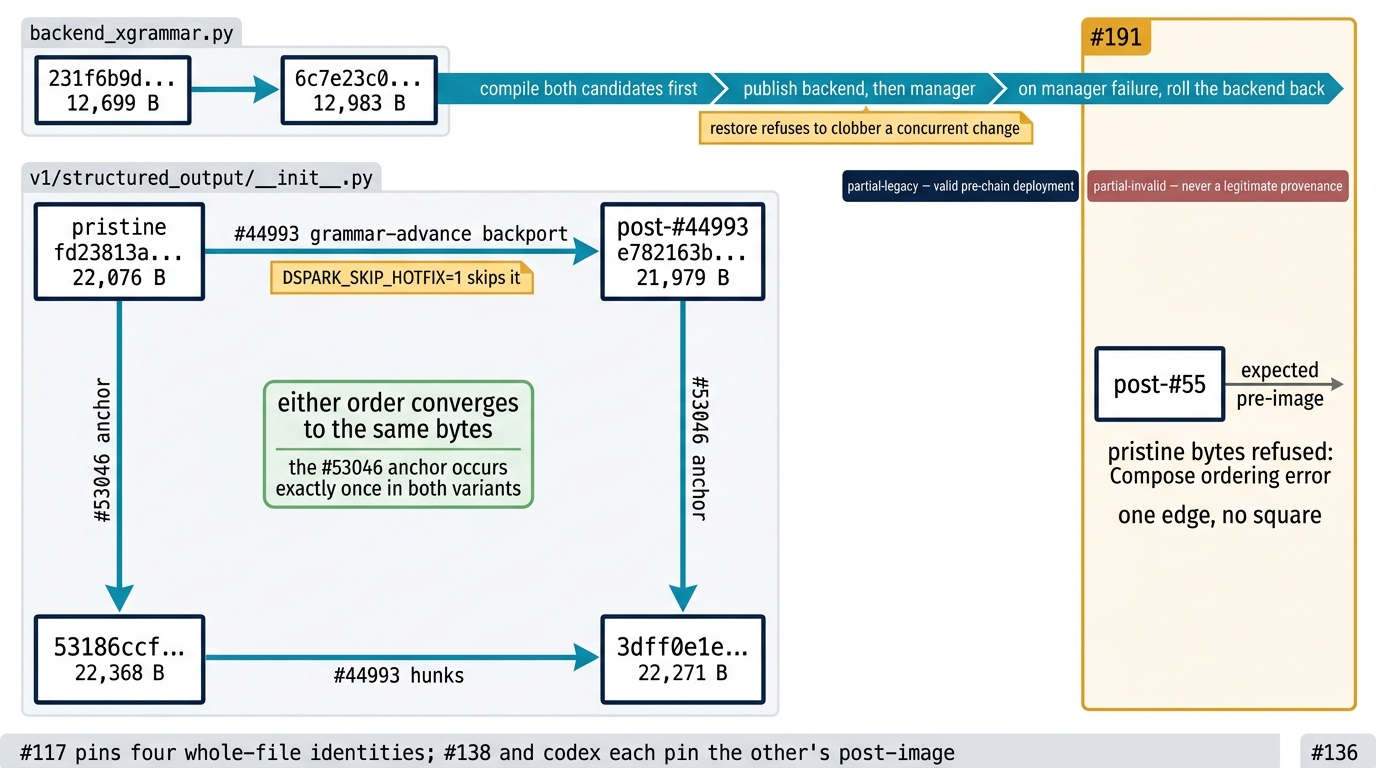
\includegraphics[width=\textwidth]{figures/ch06-multi-preimage.png}
\caption{Independent gating means every reachable boot order is a legitimate
pre-image. The \ghissue{136} chain's manager file can be met pristine
(\code{fd23813a}, 22{,}076\,B) or post-\ghissue{44993} (\code{e782163b},
21{,}979\,B) depending only on whether the operator booted with
\envvar{DSPARK_SKIP_HOTFIX}\code{=1}, so the patcher pins both with their
respective post-images, and CI proves constructively that applying the
\ghissue{44993} hunks and the \ghissue{53046} hunk in either order converges
to the same bytes. Because \ghissue{136} touches two files it also needs a
chain transaction: both candidates compiled before the first write, backend
published then manager, and a rollback that refuses to clobber a concurrent
change. Right: the contrast case --- issue \ghissue{191}'s pre-image is a
hard dependency, not a lattice.}
\label{fig:patch-multi-preimage}
\end{figure}

\section{Lifecycle: sync, recreate, upgrade}
\label{sec:patches-lifecycle}

Multiple pre-images cover what a patcher may meet on one machine --- but the
deployment runs two, and both ranks must run identical trains. The launcher
\code{scp}s every patcher
to the worker's canonical \repofile{patches/} path before starting anything.
The CI wiring gates check the worker sync list per patch, including one
sharp edge: the \repofile{vision_exp/} directory sync must
\code{rm -rf} the remote directory before \code{scp -r} so stale trees
cannot nest inside themselves.

Flag flips follow the recreate-versus-restart doctrine of
\Cref{sec:patches-strategy}: a real two-node stop/remove/start, never
\code{restart}.

The image-upgrade policy closes the loop. Because enabled mode pins exact
bytes, ``enabled mode intentionally rejects even a newer upstream file'' ---
a deliberate choice. On an image upgrade the operator leaves the flag off
until the pins are re-derived, rather than letting a patcher fuzzily apply to
code it has never seen. And when upstream merges the fix, the patch is
removed \emph{whole}: for \ghissue{136}, ``once the image incorporates
PR \ghissue{52805}, remove this patcher, flag, fixtures/tests,
sync/preflight, and documentation together.''

The repository has exercised this exit path end to end. When upstream reverted the
\ghissue{50004} adaptive-top-k backport (\ghissue{51318}, for the
capture-stride corruption told in \Cref{ch:bugs}), the fork removed its port
whole, giving back the claimed 1.0\,\% end-to-end gain. Because the
pinned image's stock code is exactly the pre-\ghissue{50004} state, removal
restored the upstream post-revert state precisely. Upstream later re-landed
the optimization capture-safely (\ghissue{52823}, 2026-08-21), but with no
capture-safe variant portable to this image, the fork stayed on stock. The
CI transaction inventory --- the frozen record of every production hunk ---
records the removal explicitly, so test coverage could not silently shrink
around the deleted patch.

\section{CI enforcement: the wiring gate and its honest limits}
\label{sec:patches-ci}

None of the above discipline survives contact with contributors unless it is
enforced mechanically. The gate that follows has two halves worth keeping
apart: what it proves about the recipe --- wiring, byte transformations,
transaction semantics, ordering --- and what it structurally cannot prove,
because it never executes a GPU kernel or runs on the arm64 platform the
patches ultimately land on. \repofile{scripts/ci-validate.sh} (562 lines, the same
script GitHub Actions runs) is that enforcement: shell syntax over every
script, \code{py_compile} over every patcher \emph{and} every test, roughly
33 hermetic CPU suites, and then a battery of regression-guard greps that
read like the project's institutional memory --- nearly every failure message
names the incident that created it.

The structural core is the four-part patch-governance invariant, demanded per
patch: \emph{default-off env gate, exact-\code{1} comparison,
\code{|| exit 1} fail-closed invocation, worker \code{scp} sync}. Each of
the four properties is independently grepped for every gated hotfix, plus
per-patch specifics (the \ghissue{138} worker env line must appear
exactly four times; the redaction patch must sit outside the skippable loop).
Greps are backed by behavior: the wiring suites extract the \emph{real}
compose entrypoint lines and execute them against recording \code{python3}
stubs, proving that enabled steps run in order, that any step's failure
blocks all later steps and the service \code{exec}, and that a flag value of
anything but exact \code{1} never invokes a gated patcher.

The strongest provenance claim in the repository anchors the hermetic patch
suites: the \ghissue{117} post-image fixture is verified equal, by Git
blob SHA-1, to the official upstream merge. Around that anchor, the suites
rest on fixture triangulation. Checked-in fixtures of the pinned vLLM
sources are locked by SHA-256 and byte length, and three independent legs
--- fixture hashes, the patcher's own pinned constants, and hunk literals
duplicated inside the test --- must agree. Replacing the test-local hunks in
the stock fixture must reproduce the post fixture byte-for-byte, so fixture,
patcher, and test check one another
(\Cref{fig:patch-fixture-triangulation}).

The transaction harness goes further. It parses the production \code{patch(...)}
calls out of each shell script's heredoc via AST, generates synthetic trees
from them, and pins every hunk in a frozen inventory (so deleting a production
hunk cannot shrink its own coverage). It then injects faults --- a
monkey-patched \code{os.replace} that fails at the $N$-th call, corrupted
re-reads, a \code{KeyboardInterrupt} mid-verification --- to prove rollback
restores bytes \emph{and} permission bits in reverse order.

The limits are stated as plainly as the guarantees. The gate is CPU-only:
``Does NOT run the live 2$\times$ Spark serve, decode bench, or
tool-eval-bench.'' It executes no GPU kernel and never touches the arm64
GB10 platform the patches ultimately run on, so it can prove the \emph{recipe}
--- wiring, byte transformations, transactions, fail-closed semantics ---
but not the runtime behavior of the patched kernels. The repository is careful not
to blur that line: the \ghissue{136} changelog entry explicitly ``does not
claim the live incident closed'' until a two-rank canary and log/health gate
pass, and the \ghissue{141} entry lists exactly which live validations remain
outstanding. Live evidence belongs to the verification scripts and canaries
of \Cref{ch:measurement}; CI's job is to make sure that what boots is exactly
what was reviewed.

\begin{figure}[htbp]
\centering
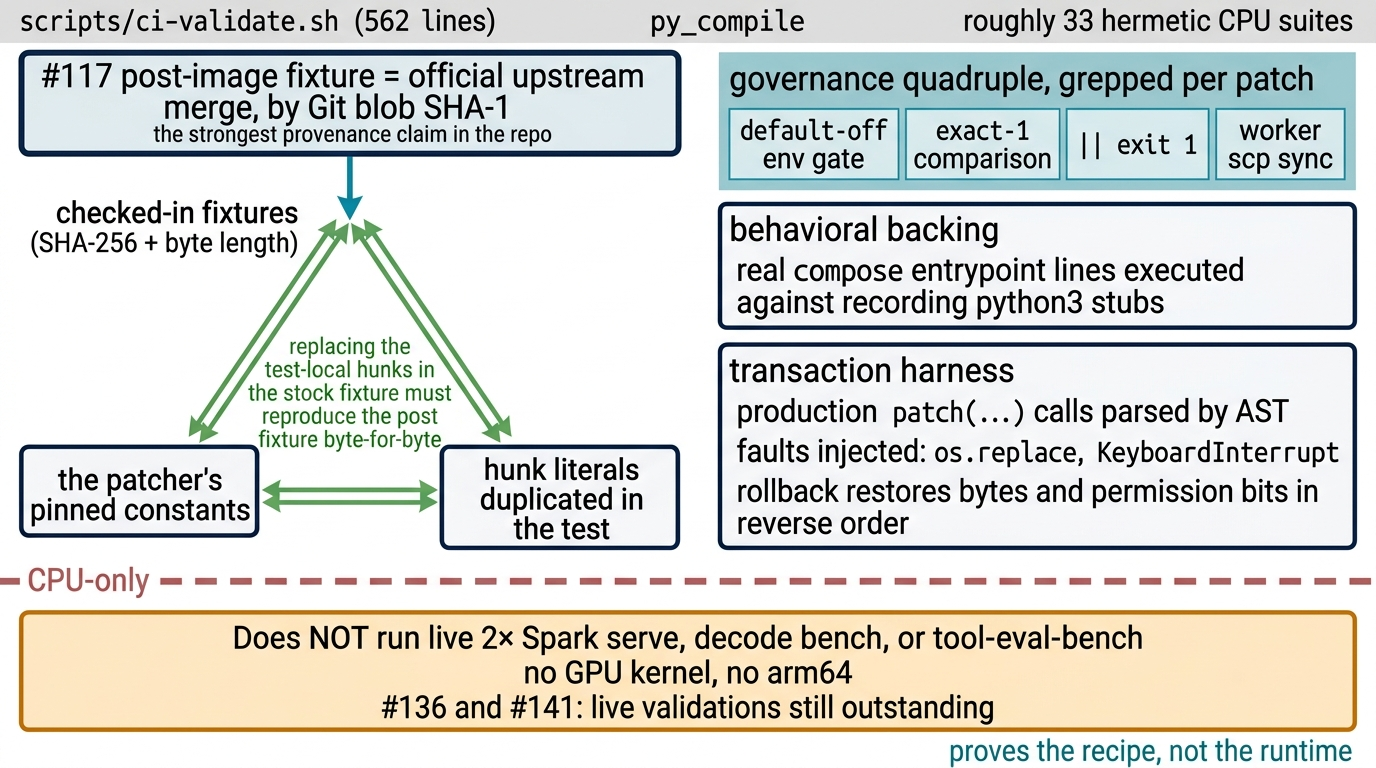
\includegraphics[width=\textwidth]{figures/ch06-fixture-triangulation.png}
\caption{The hermetic patch suites close on themselves: fixture hashes, the
patcher's pinned constants, and hunk literals duplicated inside the test must
all agree, and replacing the test-local hunks in the stock fixture must
reproduce the post fixture byte-for-byte --- anchored externally by the
\ghissue{117} post-image fixture verified equal by Git blob SHA-1 to the
official upstream merge. Around that core, the governance quadruple is
grepped per patch and backed behaviorally by executing the real compose
entrypoint lines against recording stubs, while the transaction harness
injects faults to prove reverse-order rollback of bytes and permission bits.
Below the dashed line is what a CPU-only gate structurally cannot reach: no
GPU kernel, no arm64 GB10, and no claim that a live incident is closed.}
\label{fig:patch-fixture-triangulation}
\end{figure}

A digest looked, at the start of this chapter, like the end of a provenance
question. It is the beginning of one. What a rank actually runs is that
digest plus a corpus of forty-odd transformations, applied in whatever order
the operator's flags select, into a writable layer that outlives every
\code{docker restart} --- which is why the hard engineering here lives in the
invocation and the pre-image sets rather than in the diffs. The unit of trust
shifted accordingly: not ``is this patch correct?'' but ``is every reachable
provenance enumerated, and is every failure of this patch reachable?'' A fix
nobody can prove was applied, and a failure nothing can surface, are the same
thing as no fix at all.

\FloatBarrier
\section*{Takeaways}
\begin{itemize}
\item Pinning an upstream image by manifest digest and patching it at
  container start buys byte-exact provenance, small reviewable diffs, and
  rollback-by-recreate --- at the price of writable-layer hidden state.
  Restart is not rollback; every flag change is a two-node recreate.
\item Match verification rigor to blast radius --- anchor+marker replaces for
  additive tweaks, whole-script transactions for multi-hunk backports, and
  SHA-256 pre/post-image (or AST-extracted-method) locks with version pins
  wherever drift could mean silent wrong behavior --- and give every family
  the same mechanics: never write before everything validates and compiles in
  memory, publish atomically, re-verify what you published, roll back in
  reverse order, and make a failed rollback loud, not quiet.
\item Gate opt-ins on the exact string \code{"1"}, default anything unproven
  to off, and chain every step with \code{|| exit 1}. Bare semicolons in an
  entrypoint are a latent incident (issue \ghissue{107}): a masked patch
  failure means serving stale code silently. And make \code{--status} tell
  the truth behaviorally, not by marker grep --- ``a hotfix whose
  \code{--status} lies is worse than no hotfix.''
\item Independent opt-ins that touch the same file must pin every legitimate
  pre-image (pristine \emph{and} post-sibling-patch) and prove order
  convergence; multi-file patches need chain transactions whose rollback
  refuses to clobber concurrent changes. Plan the exit on the way in, too:
  enabled mode rejects even a newer upstream file, and when upstream merges
  the fix, the patcher, flag, fixtures, tests, sync, and docs are removed
  together.
\item Enforce the governance quadruple --- default-off, exact-\code{1},
  fail-closed, worker-synced --- mechanically in CI, and be explicit about
  what a CPU-only gate cannot prove: no GPU, no arm64, no live incident
  closure.
\end{itemize}

\chaptertransition{A patch train is a machine for applying answers, and it
says nothing about the questions. Every one of those forty-odd corrections
was bought by an incident, and so was the machinery itself --- the byte pins,
the behavioral status checks, the refusal to guess at a pre-image are each
the scar of a specific failure that a looser method had already let through.
So the next chapter opens the museum: what actually went wrong, filed as
symptom, root cause, fix, and evidence. It begins with the incident that
gives the whole catalog its signature --- eight streams at 32K in which the
worst decode lane fell to 0.36 tokens per second while the preemption
counter, and every other counter an operator thinks to watch, read exactly
zero.}

% =============================================================================
% Chapter 7 — Bug Chronicles: A Field Guide to Production Failures
% Sources: repo docs/PATCHES.md, repo CHANGELOG.md, book-notes/patches-digest.md,
% book-notes/results-ops-digest.md
% =============================================================================

\chapter{Bug Chronicles: A Field Guide to Production Failures}
\label{ch:bugs}

At 32K prompts across 8 streams, the worst decode lane in this deployment
fell to 0.36~\tokspersec{} --- while the preemption counter stayed at exactly
zero. Nothing crashed, nothing was preempted, and every counter an operator
would normally watch reported a healthy scheduler; the starvation was real
and completely invisible. The root cause turned out to be a configuration
field that stock vLLM defines, documents, and defaults --- and that the
scheduler never reads. That incident (issue \ghissue{27}) is the first
exhibit in this chapter, and its shape --- a failure with no signal, traced
to an assumption nobody had verified --- recurs in almost every exhibit that
follows.

Every inference deployment eventually accumulates a private museum of
failure, and this repository's is unusually well curated: each incident filed
with a symptom, a root cause, a fix, and the measured evidence that the fix
worked --- or an honest admission that it has not yet been proven. This
chapter walks the museum thematically, but the point is never the individual
bug. Each one stands in for a general failure class --- a config field nobody
enforces, a cache keyed by the wrong identity, state frozen at CUDA-graph
capture time, an HTTP 400 that poisons a conversation forever --- that any
engineer serving large models will meet again under a different name. The
mechanics of \emph{how} these patches are applied safely is
\Cref{ch:patches}'s subject; here we study what went wrong and why, because
this catalog is the cheapest experience on offer.

\section{Scheduler starvation and fairness}
\label{sec:bugs-scheduler}

\subsection{Issue \ghissue{27}: a config field that nobody reads}

\textbf{Symptom.} With chunked prefill, async scheduling, and
\code{max_num_seqs} at 8, concurrent long prompts made already-decoding
requests crawl: at 32K prompts $\times$ 8 streams the worst decode lane fell to
0.36~\tokspersec{}, and at 8K to 2.07~\tokspersec{} --- while the preemption
counter stayed at exactly zero.

\textbf{Root cause.} Stock vLLM 0.25.2.dev0 \emph{defines}
\code{SchedulerConfig.max_num_partial_prefills} (default 1) --- but the v1
\code{Scheduler.schedule} admission loop never reads it. Multiple
admitted-but-still-prefilling requests at the front of \code{self.running} each
consume up to \code{max_num_batched_tokens} per step; decode-active requests
behind them compute \code{num_new_tokens == 0} and are skipped with
\code{continue}, not preempted. The starvation is cold-only, zero-preemption,
and grows with prompt length --- invisible to every counter an operator would
normally watch (\Cref{fig:bugs-starvation}).

\textbf{Fix.} Two coupled changes were required, and the recipe ships them
together:
\begin{itemize}
  \item \repofile{patches/hotfix-dsv4-issue27-partial-prefill-concurrency.py}
    breaks the waiting-admission loop once in-flight partial prefills reach a
    cap --- the image rejects \code{--max-num-partial-prefills}, so the cap
    arrives through \envvar{DSPARK_MAX_INFLIGHT_PREFILLS} (clamped 1--3);
  \item \envvar{LONG_PREFILL_TOKEN_THRESHOLD} is set to 1024 so each
    prefill chunk leaves budget for decode lanes.
\end{itemize}
Live evidence: 8K/16K/32K $\times$ 8 worst decode recovered to
${\sim}15$~\tokspersec{} with zero added preemptions and MTP acceptance
intact.

\begin{figure}[htbp]
\centering
\begin{tikzpicture}[node distance=3.5mm and 12mm,font=\small]
  \node[hbwarn,text width=74mm,align=left] (p1)
    {P1 --- prefill, 32K prompt, front of list:\\scheduled 8192 tokens (whole budget)};
  \node[hbfaint,text width=74mm,align=left,below=of p1] (p2)
    {P2 --- prefill: 0 tokens this step};
  \node[hbfaint,text width=74mm,align=left,below=of p2] (d1)
    {D5 --- decode-active: 0 tokens $\rightarrow$ \texttt{continue} (skipped)};
  \node[hbfaint,text width=74mm,align=left,below=of d1] (d2)
    {D6 --- decode-active: 0 tokens $\rightarrow$ \texttt{continue} (skipped)};
  \begin{scope}[on background layer]
    \node[hbgroup,fit=(p1)(d2)] (grp) {};
  \end{scope}
  \node[hblabel,anchor=south west] at (grp.north west)
    {\texttt{self.running} --- scheduled in list order};
  \node[hbbox,right=20mm of p1,text width=28mm,align=center] (bud)
    {token budget\\8192 per step};
  \draw[hbfail] (bud.west) -- node[hblabel,above=1.4mm,pos=0.5,font=\tiny]{drained by P1} (p1.east);
  \draw[hbarrow,dashed] (bud.south) |- node[hblabel,below=1mm,pos=0.6]
    {nothing left for decode lanes} (d1.east);
\end{tikzpicture}
\caption{Decode starvation under issue \ghissue{27}. One prefill at the front of
the running list consumes the entire per-step token budget; decode-active lanes
compute zero new tokens and are skipped without preemption, so no counter
records the starvation. The fix caps in-flight partial prefills at admission
and limits each prefill chunk to 1024 tokens.}
\label{fig:bugs-starvation}
\end{figure}

\subsection{Issue \ghissue{43}: the per-lane decode floor}

The \ghissue{27} cap cured per-step starvation (worst inter-token latency fell
from 2{,}790\,ms to 67\,ms), but the reporter's cold retest still showed a wide
\emph{whole-request} decode-rate spread. The follow-up patch
(\repofile{patches/hotfix-dsv4-issue43-decode-fairness-and-diag.py}) adds a
per-step service floor: when a prefill chunk is being sized, the scheduler
walks the rest of \code{self.running}, reserves
\code{num_sampled_tokens_per_step} tokens for every decode-active lane, and
caps the chunk at whatever budget remains --- dropping it to zero if the floor
cannot be met, so decodes run first. The same patch adds per-step scheduling
diagnostics behind \envvar{DSPARK_ISSUE43_SCHED_DIAG}, because the original
bug had demonstrated that this failure class produces no signal otherwise.

A
companion fix (\ghissue{105}) moved parsing of the cap's environment value out
of the admission loop and into scheduler construction, so a malformed value
warns once instead of crashing scheduling after traffic arrives.

\subsection{The default that flip-flopped: \#27 \texorpdfstring{$\rightarrow$}{->} \#154 \texorpdfstring{$\rightarrow$}{->} \#211}

The cap's \emph{value} became a saga of its own (\Cref{fig:bugs-flipflop};
the figure carries the numbers quoted at each flip). Four reversals follow,
spread over three weeks, each backed by a live A/B. The subject is not really
which cap value is right; it is what happens to a sequence of measurements
when the mechanism being measured is itself defective.

On 2026-08-19 the default went from 1 to 2 on the strength of a live A/B:
raising the cap roughly tripled 32K$\times$c4 per-stream decode with no
added preemptions --- a pure throughput argument.

On 2026-08-28, issue \ghissue{154} reversed it. A same-code fresh-boot A/B
measured four-lane 8K fairness spreads (fastest lane over slowest) two to
three times wider at cap 2 than at cap 1: the throughput had been bought
from the slowest stream.

On 2026-09-02 a more careful A/B harness flipped the default back to 2 ---
TTFT spread, worst-stream TTFT, and wave aggregate all favored the higher
cap --- an apparent reversal of \ghissue{154}'s verdict.

Then PR \ghissue{211} exposed why the evidence had been contradictory all
along: the r2 hotfix counted in-flight prefills from the stock
\code{_inflight_prefills} bookkeeping set, which could undercount, so the
``cap 2'' arms had sometimes admitted more overlap than their label claimed.
The r3 repair derives the count directly from \code{self.running} in exact
parity with the stock set's semantics: requests admitted in earlier steps
count while \code{num_computed_tokens < num_prompt_tokens}; requests
admitted this step count by the set's own add predicate; decoders can never
qualify; and a bounded tripwire logs if the stock set ever truly loses a
running partial prefill.

On 2026-09-04 the default returned to 1: all post-r3 live qualification ran
at cap 1, holding tight fairness spreads with zero preemptions across
repeated fresh-boot gate runs. The changelog explicitly notes that
the 2026-09-02 A/B favoring 2 ran on the pre-r3 \emph{undercounting}
scheduler and therefore establishes nothing about post-r3 behavior.

\begin{figure}[htbp]
\centering
\begin{tikzpicture}[font=\small]
  \draw[hbarrow,thick] (-0.4,0) -- (14.0,0);
  \foreach \x/\evtdate in {0.7/{Aug 12}, 3.9/{Aug 19}, 7.1/{Aug 28}, 10.3/{Sep 2}, 13.2/{Sep 4}} {
    \draw[hbSteel,thick] (\x,-0.09) -- (\x,0.09);
    \node[hblabel] at (\x,0.35) {\evtdate};
  }
  \node[hbnode,font=\scriptsize,text width=22mm,align=left,anchor=north] (e1) at (0.7,-0.5)
    {\ghissue{27} fix lands; cap = stock 1.\\32K$\times$8 worst decode 0.36 $\rightarrow$ 15 tok/s};
  \node[hbpatch,font=\scriptsize,text width=22mm,align=left,anchor=north] (e2) at (3.9,-0.5)
    {default $\rightarrow$ 2.\\32K$\times$c4 decode 8.2 $\rightarrow$ 24.6 tok/s};
  \node[hbgpu,font=\scriptsize,text width=22mm,align=left,anchor=north] (e3) at (7.1,-0.5)
    {default $\rightarrow$ 1 (\ghissue{154}).\\spread 3.7--5.1$\times$ at 2 vs 1.7--2.0$\times$ at 1};
  \node[hbpatch,font=\scriptsize,text width=22mm,align=left,anchor=north] (e4) at (10.3,-0.5)
    {default $\rightarrow$ 2.\\TTFT spread 9.1 vs 14.6 s, +12\,\% agg.\ (pre-r3 counter)};
  \node[hbgpu,font=\scriptsize,text width=22mm,align=left,anchor=north] (e5) at (13.2,-0.5)
    {default $\rightarrow$ 1 (\ghissue{211} r3 exact count).\\spread 1.60--1.76$\times$, 0 preempt.};
\end{tikzpicture}
\caption{The \envvar{DSPARK_MAX_INFLIGHT_PREFILLS} default flip-flops, with the
evidence quoted at each flip. Amber boxes raise the cap for throughput; green
boxes lower it for fairness. The final flip is the decisive one: \ghissue{211}
showed the earlier ``cap 2'' measurements ran on an undercounting admission
counter, so their labels did not describe the schedule actually executed.}
\label{fig:bugs-flipflop}
\end{figure}

\begin{hblesson}
Two lessons. A configuration field that exists but is never enforced is worse
than one that does not exist: operators tune it, document it, and A/B it, and
every conclusion is fiction --- verify enforcement by observing behavior.
And before trusting an A/B, verify the knob's \emph{mechanism} is intact:
every pre-r3 fairness measurement carried a silent confound, and the honest
response was to re-qualify from scratch, not average the old results.
\end{hblesson}

\section{Cache correctness}
\label{sec:bugs-cache}

Issue \ghissue{27} was a knob that steered nothing; the museum's next wing
holds the inverse hazard --- expressions that steered everything. The two
exhibits in this section share a shape: a single small expression
--- a dtype string compared against the wrong literal, a hit count reduced
with the wrong min --- silently steering the entire cache layer, correct on
every short test and wrong at scale.

\subsection{Issue \ghissue{22}: the sixteen-fold dispatch typo}

\textbf{Symptom.} With the recipe-default \code{--kv-cache-dtype nvfp4_ds_mla},
decode throughput at 600K+ context collapsed to ${\sim}1.0$~\tokspersec{}, while
\code{fp8_ds_mla} sustained ${\sim}17.3$~\tokspersec{} at the same length.
Short-context throughput was unaffected --- so every smoke test passed.

\textbf{Root cause.} A one-line dispatch condition:

\begin{lstlisting}[language=Python]
# flashmla_sparse.py, line ~880 -- the whole bug
use_fp8_cache = self.kv_cache_dtype == "fp8_ds_mla"
# nvfp4_ds_mla -> False -> slow _forward_bf16_kv  (~1 tok/s at 600K)
# fp8_ds_mla   -> True  -> fast _forward_fp8_kv   (~17 tok/s at 600K)

# fix
use_fp8_cache = self.kv_cache_dtype in ("fp8_ds_mla", "nvfp4_ds_mla")
\end{lstlisting}

On DSV4 the 584-byte-per-token KV layout is byte-identical for both dtypes;
only the kernel dispatch differed, so routing nvfp4 to the fp8 kernel is
exactly correct. The class: a ``supported'' dtype can be silently routed to a
fallback kernel, and the gap opens only where nobody benchmarks --- here, at
extreme context.

\subsection{Issues \ghissue{26} and \ghissue{36}: the hybrid-cache min, broken twice}

\textbf{Symptom (\ghissue{26}).} Warm repeats of 32K+ shared-prefix prompts
$\times$ 8 streams fully re-prefilled: \code{prefix_cache_hits_total} advanced
by zero and warm wall-clock equaled cold ($\sim$421\,s instead of $\sim$9\,s
at 32K).

\textbf{Root cause.} This model runs four KV-cache groups --- one
\code{MLAAttentionSpec} plus three \code{SlidingWindowMLASpec} --- and vLLM's
\code{HybridKVCacheCoordinator.find_longest_cache_hit} takes the \emph{minimum}
hit length across groups. A sliding-window group frees old blocks by design;
once the window has slid past the prefix start, its hit length at the prefix
is zero, and the min zeroes the common hit even though the MLA group holds the
entire history (\Cref{fig:bugs-hybridmin}).

\textbf{The overcorrection (\ghissue{36}).} The v1 fix skipped SWA groups in
the min, letting the long MLA hit survive. Hit \emph{rates} recovered ---
and then a 21K-token Hermes-style shared system prefix began decoding garbage:
leftover DSML fragments, Chinese characters, loops. The v1 patch had let the
engine report a 100\,\% hit, skip prefill entirely, and attach \emph{null} SWA
KV for a window position the cache genuinely no longer held. Different user
turns move the replay boundary, so the corruption was intermittent and warm-only.

\textbf{Fix (v2).} Restore the stock min semantics --- SWA may shrink the
common hit again --- and move the warm-hit win to a different mechanism.
\envvar{VLLM_PREFIX_CACHE_RETENTION_INTERVAL}\,=\,4096 keeps one sparse SWA
tail checkpoint per 4096-token segment, so the min lands on the last retained
tail instead of zero. The design note in the patch is the right mental model:
``a 21k prefix may cache ${\sim}$20k instead of 21k; that is correct.'' Live
evidence: warm $\times$8 runs at ${\sim}$22.8K/44.7K/88.4K tokens all 8/8 with
warm-to-cold ratios 0.9973--0.9996, and the 32K warm wall fell from
${\sim}$421\,s to ${\sim}$9\,s.

\begin{figure}[htbp]
\centering
\begin{tikzpicture}[font=\scriptsize]
  % MLA row
  \node[hblabel,anchor=east] at (-0.3,0) {MLA group};
  \foreach \i in {0,...,9} {
    \node[hbgpu,minimum width=6mm,minimum height=5mm,inner sep=0pt]
      at (\i*0.72,0) {};
  }
  \node[hblabel,anchor=west] at (7.1,0) {full 21k prefix retained};
  % SWA row
  \node[hblabel,anchor=east] at (-0.3,-0.9) {SWA groups};
  \foreach \i in {0,...,7} {
    \node[hbfaint,minimum width=6mm,minimum height=5mm,inner sep=0pt]
      at (\i*0.72,-0.9) {};
  }
  \foreach \i in {8,9} {
    \node[hbgpu,minimum width=6mm,minimum height=5mm,inner sep=0pt]
      at (\i*0.72,-0.9) {};
  }
  \node[hblabel,anchor=west] at (7.1,-0.9) {old blocks freed; only tail live};
  % outcomes
  \node[hbwarn,text width=124mm,align=left,anchor=north] at (5.0,-1.7)
    {stock: hit = min across groups = 0 $\rightarrow$ warm shared-prefix runs
     fully re-prefill; warm wall $\approx$ cold (\ghissue{26})};
  \node[hbwarn,text width=124mm,align=left,anchor=north] at (5.0,-2.75)
    {v1 fix: exempt SWA from the min $\rightarrow$ 21k ``hit'' with null SWA KV
     $\rightarrow$ DSML/CJK output salad on warm shared prefixes (\ghissue{36})};
  \node[hbgpu,text width=124mm,align=left,anchor=north] at (5.0,-3.85)
    {v2: restore the min + retention checkpoints every 4096 tokens
     $\rightarrow$ hit stops at the last retained SWA tail ($\sim$20k) --- correct
     and warm (ratios 0.997--0.9996)};
\end{tikzpicture}
\caption{Issue \ghissue{26}: hybrid prefix-cache hit computation across
heterogeneous KV groups. The MLA group retains everything; sliding-window
groups free blocks by design, so the min-across-groups hit collapses to zero
(stock), or --- if SWA is simply exempted --- reports a hit backed by KV that no
longer exists (v1, issue \ghissue{36}). The v2 design keeps the min honest and
retains sparse SWA tails so it lands somewhere useful.}
\label{fig:bugs-hybridmin}
\end{figure}


\begin{hbwarning}
When a cache-hit computation spans components with different retention
policies, the only safe answers are the honest minimum or a retention scheme
that guarantees the reported hit is materialized in \emph{every} component.
Reporting the optimistic maximum converts a performance bug into a
silent-correctness bug --- strictly worse.
\end{hbwarning}

\section{Rendering dead states}
\label{sec:bugs-render}

The cache exhibits corrupted what the engine remembered. Issue \ghissue{52}
corrupted what the model was asked to do next: it handed the generator a
prompt with nowhere legal to go. The class is coverage of transcript shapes:
an encoder has to yield a legal continuation point for every message sequence
a client may legally send, and any shape it leaves without a generation
header becomes a state the model cannot generate its way out of.

\textbf{Symptom (\ghissue{52}).} An agent harness got stuck emitting empty
turns: one or two generated tokens, \code{finish_reason: "stop"}, no tool
call, fragments of hallucinated markup. In one live incident, 6 of 37 requests
generated ${\leq}10$ tokens --- all \code{stop}, zero \code{length}.

\textbf{Root cause.} The checkpoint's encoder (\code{render_message()} in
\repofile{encoding/encoding_dsv4.py}) appends the generation header only when
the trailing message is \code{user} or \code{developer}. A request whose
\code{messages} array ends with an \emph{assistant} message is closed with EOS
and gets no header: the prompt ends on a bare EOS and the model generates from
a dead, turnless state. Worse, the failure is self-sustaining --- the harness
records the empty turn, so the next request is also assistant-final.

\textbf{Fix.} The opt-in patcher
\repofile{patches/hotfix-dsv4-assistant-final-continuation.py} --- gated by
\envvar{DSPARK_ENABLE_ASSISTANT_FINAL_HOTFIX} --- widens the transition condition:
a final assistant message keeps its EOS-closed turn and gains a fresh
generation header. The alternative --- reopening the turn without EOS --- was
measured and rejected: reopening a \emph{complete} turn just relocates the dead
state (a 1-token empty generation), while EOS-plus-header produced healthy
continuations for both partial and complete trailing turns.

Issue \ghissue{120}
later extended the same fix by exactly one clause: a harness retry can append a
trailing \code{latest_reminder} annotation after the re-sent assistant turn,
which again left the prompt headerless. A final reminder whose immediate
predecessor is an assistant message now also gains one header. Reminder tails
after \code{user}/\code{developer} already end inside the pending generation
slot and stay byte-identical; the patcher's post-write self-check fails closed
if a patched encoder ever double-headers that shape.

\textbf{Evidence --- including a failure of the fix itself.} The causal
evidence is a one-prompt A/B via \code{/v1/completions}: trailing turn left
open $\rightarrow$ 183 tokens of coherent continuation; closed with EOS
$\rightarrow$ 400 tokens of raw \code{<|DSML|tool_calls>} markup emitted as
text. The repository states plainly that there is \emph{no rescue claim}: the live
no-op loop did not reproduce in the test session, so no measured
stuck-harness recovery exists.

And the first gated-ON boot failed closed
before serving: a review-requested guard referenced a checkpoint variable
named \code{add_generation_prompt} that does not exist in this encoder, so the
patcher restored the original bytes and aborted. The corrected commit then
passed a serialized live OFF/ON proof on both ranks: OFF rendered stock EOS; ON
preserved all 98 stock token IDs and appended exactly the assistant-thinking
header, completed a live continuation, and verified idempotence on re-run. A
deliberate anchor-drift boot exited 1 on both ranks without ever serving.
The \ghissue{120} extension's evidence is CPU-only so far (a 16-case render
matrix on the real encoder snapshot); the docs demand the same two-rank boot
proof before relying on it.

\begin{hbwarstory}
The guard that named a nonexistent variable is the quiet hero here. A
conventional patch train would have served a corrupted encoder; the
fail-closed contract (verify, else restore bytes and refuse to boot) turned a
latent correctness bug into a loud startup failure. The repository's principle: an
enabled boot must never silently serve stock behavior --- and a failed patch
must never serve half-patched behavior.
\end{hbwarstory}

\begin{figure}[htbp]
\centering

\includegraphics[width=0.80\textwidth]{figures/toon-ch07-quiethero.png}
\caption{The smallest thing holding back the largest. The guard that named a nonexistent variable had no business working, and it is the reason a corrupted encoder never reached a user: the fail-closed contract turned a latent correctness bug into a loud startup failure. An enabled boot must never quietly serve stock behaviour, and a failed patch must never serve half-patched behaviour.}
\label{fig:toon-quiethero}
\end{figure}

\section{Tool-call integrity}
\label{sec:bugs-toolcalls}

The assistant-final loop was self-sustaining because the harness recorded
the empty turn and sent it back --- a first taste of the dynamic this wing
meets at full strength. Tool calling stresses the API layer harder than
plain chat, because clients
\emph{replay} what the server said: a single malformed response poisons every
subsequent turn of the conversation.

\subsection{Issue \ghissue{21}: dict arguments, double-encoded}

Multi-turn tool calling failed after the first successful tool turn: prior
assistant tool calls were re-encoded into the prompt with a single wrapped
\code{arguments} key instead of the real parameter keys, and the model then
imitated the corrupt history. Root cause, in the upstream HF checkpoint's
encoder: \code{encode_arguments_to_dsml} always calls \code{json.loads}
on \code{tool_call["arguments"]}. When \code{arguments} is already a
dict --- a legal shape in OpenAI-compatible replay --- \code{json.loads}
raises, and the blanket \code{except} wraps the dict as
\texttt{\{"arguments": <dict>\}}. The fix dispatches on type before parsing.
Notably, the bug lived in the checkpoint's own encoding file, not in vLLM or
the recipe weights.

\subsection{Issue \ghissue{55}: truncation that lies, and an enum that never matched}

Issue \ghissue{21} corrupted the replayed history by an accident of type
handling; issue \ghissue{55} did it by reporting a truncation as a success.

\textbf{Symptom.} When \code{max_tokens} cut a request mid-tool-call, stock
vLLM still reported a finish reason of \code{tool_calls}, and the streaming
flush delivered arguments that were not valid JSON:

\begin{lstlisting}
finish_reason: "tool_calls"      <- engine actually stopped on LENGTH
arguments: '{"path": "/tmp/log.txt", "content": "'   <- unterminated JSON
\end{lstlisting}

A harness that replayed the broken call had its whole transcript rejected with
HTTP 400 on every later turn --- the reporter's ``poisoned conversation''
chain. The hotfix reports finish reason \code{length} for truncated calls
(streaming and non-streaming) and drops tool calls whose arguments do not
parse; natural-stop calls are untouched. The live A/B confirmed every
truncation cell flipped from \code{tool_calls} to \code{length} while
non-truncated cells kept valid calls. Streamed argument fragments cannot be
recalled --- the OpenAI stream protocol is append-only --- so the protection is
the correct terminal signal, which spec-compliant clients use to discard the
in-flight call.

\begin{hbnote}
\textbf{Dead code since upstream: the comparison that never matched.} While
auditing for regressions, the author found that vLLM's \code{FinishReason}
is an \code{IntEnum}, not a \code{StrEnum} --- so the stock code comparing
\code{output.finish_reason} to \code{"stop"} at \repofile{serving.py}
line 961 had \emph{never} matched. The \code{tool_choice="required"}
natural-stop branch it guarded had been dead since the day upstream shipped
it. The same audit showed \code{FinishReason.ABORT} and \code{REPETITION}
would reach clients serialized as \code{'2'} and \code{'4'} rather than
their names; the hotfix's \code{str(...)} coercion fixed that latent bug
too.
\end{hbnote}

\subsection{Issue \ghissue{191}: the 142/145 that was not a grammar bug}

Truncation returns in this wing's last exhibit, disguised well enough to
implicate an entirely different subsystem.

\textbf{Symptom.} On the Vision-Exp lane (async scheduling, TP=2, MTP), the
145-case tool-calling gate scored 142/145 twice at concurrency 4: HTTP 200
responses with zero \code{tool_calls} in named and \code{required} lanes, or
arguments violating the \code{strict} schema. The failing labels changed
between runs, and every failed case replayed 18/18 clean --- the signature of a
concurrency-dependent leak, not a prompt problem.

\textbf{Root cause --- measured, and not the suspected one.} The obvious
suspect was the known fail-open hazard in structural-tag grammar masking under
speculative decoding plus async scheduling (the upstream \ghissue{49694}/%
\ghissue{54437} family). The 2026-09-03 measurement acquitted it: the
scheduler never logged a genuine grammar rejection; every
\code{Failed to advance FSM} line came from the \emph{tolerated} post-%
\code{</think>} draft check; and disabling async scheduling entirely
(a purpose-built knob, \envvar{DSPARK_ASYNC_SCHEDULING})
produced the same violation rate. The real cause: with thinking enabled at
\code{reasoning_effort=low}, a fraction of strict tool requests reason for
300--500 tokens --- non-deterministically across batches, even at temperature
0. The client's \code{max_tokens=512} therefore cut the reply before or inside
the DSML call (\code{finish_reason=length}, zero or a salvaged partial call).
Replaying the identical input mostly replays the problem.

\textbf{Fix.} An opt-in fail-closed contract layer at the serving boundary:
after generation, a named or \code{required} non-streaming response is checked
for cardinality, tool name, JSON-object arguments, and \code{strict}-schema
conformance. A violation logs a structured warning and regenerates with a
fresh engine request id, up to a bounded retry count, finally answering
HTTP 500 rather than a wrong 200. The last retry applies the
\emph{thinking-off fallback}: the prompt's trailing \code{<think>} token is
swapped for \code{</think>} --- byte-identical to rendering the chat with
thinking disabled --- so the grammar constrains the reply from its first token
and the call fits the client's budget. The acceptance bar is 145/145 on the
same gate, with the warning count in the logs as the measured raw violation
rate.

\section{Grammar meets speculative decoding}
\label{sec:bugs-grammar}

Issue \ghissue{191} acquitted the grammar stack; these two exhibits are the
cases where it was genuinely at fault --- though the guilt lies in how it
meets speculative decoding, not in the grammar engine itself. Constrained
decoding assumes the grammar FSM sees every emitted token exactly
once, in order. Speculative decoding violates that assumption in two ways this
repository hit separately.

\textbf{The \ghissue{44993} grammar-advance train (issue \ghissue{24}).}
\code{response_format json_schema} with thinking enabled produced duplicated
prefixes like \texttt{\{"city":"Paris\{"city":"Paris"\}}. Root cause:
\code{should_advance} returned False when reasoning ended mid-step for
JSON/regex/choice constraints, so the draft tokens produced right after the
reasoning-end marker never entered the grammar FSM --- and the model re-emitted
the opening token on the next step. The backported fix passes the exact
appended token ids to \code{should_advance} and records the reasoning-end
index for all constraint types.

\textbf{Issues \ghissue{136} and \ghissue{210}: tokens after termination.}
With DSpark MTP, \code{structural_tag} constraints, async scheduling, and
TP=2, one accepted draft batch can contain a terminating token \emph{followed
by} speculative tokens. The pinned vLLM passed those trailing tokens to an
already-terminated XGrammar matcher, with a characteristic log line:

\begin{lstlisting}
The matcher has terminated ... but is trying to accept new token
\end{lstlisting}

\noindent after which the request could stop progressing and eventually die in the
generic 1{,}800-second \code{sample_tokens} RPC timeout. Raising that deadline
cannot repair a desynchronized state machine.

\textbf{Fix.} The fix backports upstream
\ghissue{52805} (accept/validate stop at the terminating token, cache
termination, treat later acceptance as a no-op, clear everything on reset)
plus \ghissue{53046} (validate a post-reasoning draft before accepting it, so
a grammar-invalid draft that predates the bitmask is skipped instead of
tripping the spurious \code{Failed to advance FSM} error path). One flag
applies both as a single two-file transaction: both candidates are built and
compiled before either write, publication is per-file atomic in chain order,
and a second-file failure rolls the first back byte-exactly. Because the
\ghissue{44993} train touches the same manager file, the patcher pins both
legitimate stock identities (post-\ghissue{44993} and pristine), and the test
suite proves both application orders converge byte-exactly.

\textbf{Evidence.} The evidence status is stated with the repository's usual
discipline: no output corruption was
demonstrated for the prior code, the reporter measured their best tool-eval
result with both backports active --- and the issue is not to be claimed
closed until the two-rank live canary and log gate pass. Both fixes here are
backports of upstream corrections; the next wing inverts that relationship
--- upstream correcting this fork.

\section{Silent corruption under CUDA graphs}
\label{sec:bugs-cudagraph}

On 2026-08-22 the changelog records the most humbling entry in the museum:
upstream vLLM identified \emph{two of this repository's own performance
backports} as sources of intermittent silent output corruption under
MTP + prefix caching + CUDA graphs on 2$\times$ DGX Spark. The symptoms:
foreign-character bursts, token salad, corrupted tool calls after hours of
healthy serving, investigated publicly on the NVIDIA forums.

\textbf{The packed-stride revert (\ghissue{50004}).} The adaptive top-k-width
backport had the C128A metadata builder write packed rows at the \emph{live}
batch's stride, while FULL-graph consumers retain the \emph{capture-time}
stride. Every row beyond the first therefore read stale slot ids, and
attention landed on the wrong context slices. Upstream reverted the PR outright
(\ghissue{51318}); this fork dropped its backport from the patch train
entirely, giving back the claimed 1.0\,\% end-to-end gain, because the pinned
image's stock code is exactly the pre-\ghissue{50004} state.

\textbf{The capture-baked shortcut (\ghissue{49486}).} The short-context
indexer shortcut early-returns all candidates when the context is short enough
that top-k would select everything. This fork's port had asserted that ``the
branch is stable inside a capture.'' Upstream refuted it: a graph captured
against short \emph{dummy} metadata bakes the shortcut in, then replays it
against longer cached prefixes, returning candidates $0..\mathrm{topk}{-}1$
unscored --- wrong-context attention, intermittently, only under prefix caching
plus CUDA graphs. The port now carries upstream \ghissue{52492}'s guard
verbatim: the shortcut is barred while
\code{torch.cuda.is_current_stream_capturing()}; eager steps keep it.
\Cref{fig:bugs-capture-drift} puts the two incidents side by side.

\begin{hbwarstory}
Both corruptions share one mechanism: \emph{a decision made at capture time was
replayed against run-time state that had drifted}. A captured CUDA graph is a
recording --- every branch taken during capture is frozen, every stride and
shape baked in. The rule this repository now applies in four separate patches: no
captured path may depend on per-step CPU state, and any data-dependent
shortcut must be explicitly disabled during stream capture. The humility
lesson is real too: these were this fork's own performance patches, ported in
good faith with a written rationale --- and the rationale was wrong. Perf
backports onto a pinned image deserve the same
adversarial review as new kernels.
\end{hbwarstory}

\begin{figure}[htbp]
\centering
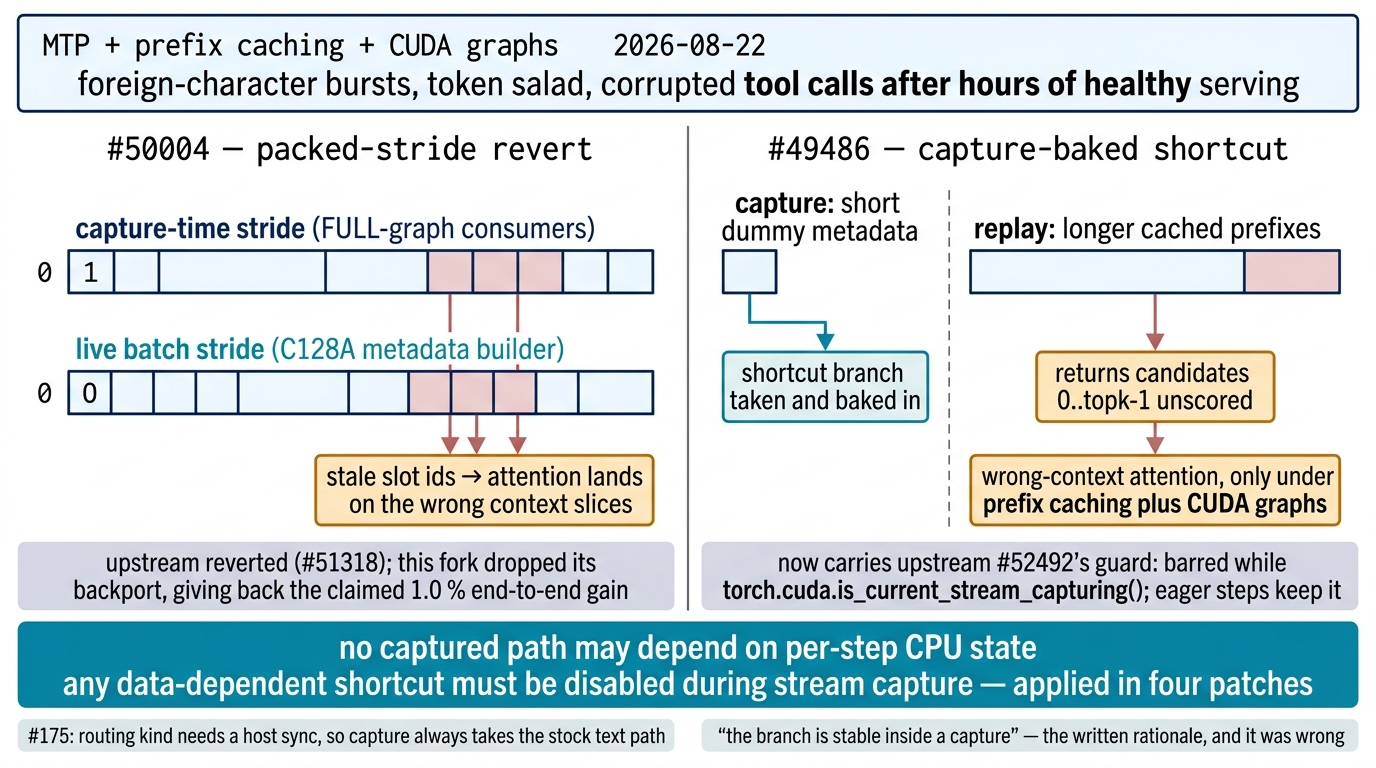
\includegraphics[width=\textwidth]{figures/ch07-capture-vs-runtime.png}
\caption{Both of 2026-08-22's silent-corruption incidents share one mechanism:
a decision made at capture time replayed against run-time state that had
drifted. Left: the adaptive top-$k$ backport (\ghissue{50004}) had the C128A
metadata builder write packed rows at the live batch's stride while FULL-graph
consumers retain the capture-time stride, so every row beyond the first read
stale slot ids --- upstream reverted it (\ghissue{51318}) and this fork dropped
its backport, giving back the claimed 1.0\,\% gain. Right: the short-context
indexer shortcut (\ghissue{49486}) is baked in by a capture against short dummy
metadata, then replayed against longer cached prefixes, returning candidates
\code{0..topk-1} unscored; the port now carries upstream \ghissue{52492}'s
guard, barring the shortcut while the stream is capturing. The rule, now
applied in four patches: no captured path may branch on per-step state.}
\label{fig:bugs-capture-drift}
\end{figure}

\section{The stochastic stall: issue \ghissue{141}}
\label{sec:bugs-stall}

The capture-time corruptions at least ended with mechanisms in hand. The
museum keeps one case that has not.

\textbf{Symptom.} A stochastic TP=2 engine death: generation silently
truncates mid-response with no terminal \code{finish_reason}, while
\code{/health} keeps returning 200. The missing \code{finish_reason} is the
earliest reliable signal --- an operator watching only health checks sees
nothing.

\textbf{What is actually known.} The failure samples inside FlashInfer's SM120
sparse-MLA paged-attention fallback. The pinned FlashInfer revision routes
calls of at most 64 rows to its standalone DSv4 decode kernel; larger calls go
to the paged/prefill orchestrator implicated in the stalls. On one reporting
pair of machines, splitting verify-decode calls at 64 rows survived
3{,}145{,}728 generated tokens, while a 65-row split failed in the first
comparison round. That is the entire causal evidence base: the second failing
pair has not repeated the A/B, and the live TP/stream mechanism remains
unknown.

\textbf{The retractions.} Issue \ghissue{143} initially blamed an
admission-cap interaction. The repository's own wording is unambiguous: the
\ghissue{143} ``\code{MAX_NUM_SEQS=16} bad / 32 safe'' admission-cap mechanism
is \textbf{RETRACTED} --- ``every cell in that matrix was $n{=}1$; per-burst
failure probability explains the whole table without an admission-cap
effect.'' The 2026-08-27 changelog records the same demotion (a single-run
hypothesis invalidated by repeated \ghissue{141} bursts), along with the
earlier framing of \code{MAX_NUM_SEQS=32} as a ``safety''
configuration. The docs now state that no tested \code{MAX_NUM_SEQS} is
generally safe and that configuration changes may alter \emph{incidence}
rather than fix the stall --- admission tuning is performance data, not a
safety recommendation.

\textbf{The workaround --- explicitly not a fix.} The default-off patcher
never makes a call larger than 64 rows (gate
\envvar{DSPARK_ENABLE_ISSUE141_SPARSE_MLA_CHUNK}): bigger calls become sequential disjoint 64-row slice views of
the same six row-coupled tensors, sharing caches, workspace, and output
allocation by identity. The fixed 64 is the pinned kernel-dispatch boundary,
not a deployment concurrency threshold. The patcher source-locks not only the
method it rewrites but also the FlashInfer fragments in a \emph{different
package} whose behavior justifies the constant. The docs enumerate the
still-open validation gates (SM121a numerical tests, a two-rank boot proof,
repeated stochastic soaks) and close with the doctrine this chapter keeps
returning to: one clean burst cannot close a stochastic issue.

\begin{hblesson}
For a stochastic failure, keep three columns: observed (a 64/65-row boundary
on one pair), inferred (path avoidance helps), and unknown (the mechanism,
and whether the second pair reproduces the boundary). Labeling the mitigation
``workaround, not root-cause fix'' in the patch itself, and retracting the
earlier hypothesis in the changelog, is the difference between a field guide
and folklore.
\end{hblesson}

\section{Infrastructure: caches, watchdogs, and spin-waits}
\label{sec:bugs-infra}

The \ghissue{141} stall is not the only way this deployment has lost a TP=2
pair mid-serve. The older way was mundane and --- unlike the stall --- was
chased to a complete root-cause chain. The three exhibits here share a
theme: work deferred until first use --- a kernel not yet compiled, a cache
not yet warm, a sleep path never taken --- costs nothing at boot and
everything under load.

\subsection{Issue \ghissue{117}: the JIT-cache death chain}

\textbf{Symptom.} Mid-serve, an entire TP=2 pair would die: one rank stalls,
the peer waits, and after ${\sim}$600 seconds torch's ProcessGroupNCCL
watchdog terminates the group. Post-mortems found zero collective-level
evidence --- the stalled rank logs nothing.

\textbf{Root cause.} A chain: the in-image Triton cache
(\repofile{~/.triton/cache}) lives in the container's writable layer and dies
on every container recreate; the next boot therefore re-JIT-compiles
already-known kernel shapes \emph{mid-serve} the first time traffic hits them;
a rank stalled in compilation leaves its TP peer parked in a collective; and
the 600-second watchdog --- a deadline that
\envvar{VLLM_EXECUTE_MODEL_TIMEOUT_SECONDS} does not extend --- kills the pair.
The field incident recorded exactly this chain from
\code{_prepare_dflash_inputs_kernel} (\Cref{fig:bugs-jit-chain}).

\textbf{Fixes, layered.}
\begin{enumerate}
  \item \emph{Persist the caches.} \envvar{TRITON_CACHE_DIR} moved onto the
    HF volume, mirroring the earlier \envvar{TILELANG_CACHE_DIR} fix from
    issue \ghissue{65}. A third cache was found later, when a validated boot
    still logged mid-serve CuTeDSL compilation --- the B12X MoE backend's
    own compile cache, now pinned via \envvar{B12X_CUTE_COMPILE_CACHE_DIR}.
    Caches that die with containers are a slow-burning fuse: everything
    works until the first recreate under load.
  \item \emph{Warm the shapes.} A post-ready boot sweep materializes the
    enumerable compile-key buckets before real traffic. It was later hardened
    into a deterministic bucket ladder of exact-token prompts mapped through
    the kernel's own \code{next_pow2} block-size formula onto all six live
    cache keys, after review showed the original concurrency-based arms
    could not reach the low buckets at all.
  \item \emph{Bound the damage.} The \ghissue{45224} backport caps an idle
    SHM ring-buffer reader's wait at 5{,}000\,ms so a missed notify
    self-recovers, and releases the reader slot in \code{finally} when a
    consumer raises.
  \item \emph{Instrument the next one.} The PyTorch flight recorder is
    pinned on, with dumps persisted to the HF volume and a named-pipe
    trigger, so a future frozen-but-not-timed-out pair can be poked for
    per-rank collective traces before restart (archive both ranks' dumps
    together --- the files truncate on every dump).
\end{enumerate}

\begin{figure}[htbp]
\centering
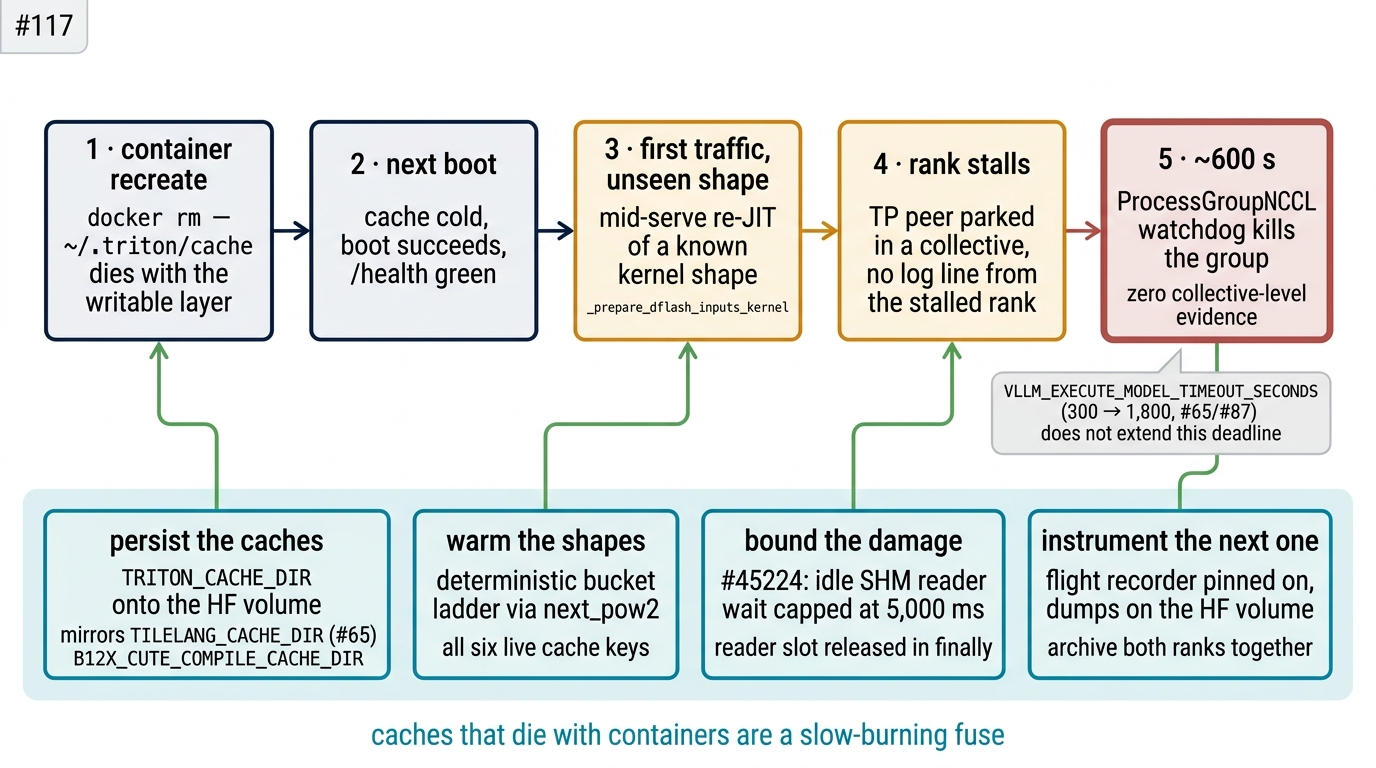
\includegraphics[width=\textwidth]{figures/ch07-jit-death-chain.png}
\caption{Issue \ghissue{117}'s chain. The in-image Triton cache lives in the
container's writable layer and dies on every recreate, so the next boot
re-JIT-compiles already-known kernel shapes mid-serve the first time traffic
reaches them --- the field incident was recorded from
\code{_prepare_dflash_inputs_kernel}. A rank stalled in compilation parks its
TP peer in a collective, and after roughly 600 seconds torch's
ProcessGroupNCCL watchdog kills the pair, leaving no collective-level
evidence; \envvar{VLLM_EXECUTE_MODEL_TIMEOUT_SECONDS} does not extend that
deadline. The four fixes each cut a different link: persist the caches, warm
the six enumerable compile keys at boot, bound the idle reader's wait at
5{,}000\,ms, and wire the flight recorder for the next one.}
\label{fig:bugs-jit-chain}
\end{figure}

\subsection{Issue \ghissue{133}: the compile-key explosion}

A subtler JIT hazard: mixed prefill slices two tensors at the same
traffic-dependent token offset, so Triton's automatic pointer-alignment
specialization produced three cache-key states for the global-top-k kernel.
Crossed with two effective block sizes, that meant six persistent-cache
entries --- and mid-serve compilation stalls whenever traffic found a new
combination. Both
pointers are scalar loads, so alignment specialization bought nothing. The fix
disables alignment specialization for exactly those two pointers and promotes
the stable strides and sizes to \code{tl.constexpr}, collapsing the family to
two deterministic variants, both compiled at boot. The class: a JIT compiler's
\emph{implicit} specialization axes (alignment, dtype, contiguity) multiply
against traffic patterns; enumerate them or they will enumerate themselves in
production.

\subsection{Issues \ghissue{79}, \ghissue{65}, and \ghissue{87}: the small stuff that compounds}

vLLM's cross-process IPC wait spun on \code{busy_loop_s = 1} before sleeping.
Under decode the message gap is always shorter, so the sleep path never
engaged and three to four Grace P-cores spun at max clock, stealing SoC power
budget from the GPU --- fixed by one value, 1\,s $\rightarrow$ 2\,ms
(\ghissue{79}). And \envvar{VLLM_EXECUTE_MODEL_TIMEOUT_SECONDS} was raised
from the stock 300 to 1{,}800 so a legitimate mid-serve TileLang/CuTeDSL JIT
does not get the engine killed while it compiles (\ghissue{65}/\ghissue{87})
--- a stopgap the persisted caches and warmup sweep then made mostly moot.

\section{Vision-Exp integration bugs}
\label{sec:bugs-vision}

The poisoned-transcript dynamic of \Cref{sec:bugs-toolcalls} returns for the
museum's final wing --- the same replay dynamic, in a new subsystem.
Grafting a vision tower onto a text-only serving stack produced its own bug
family --- almost entirely in \emph{validation and identity} logic, not in the
neural network.

\subsection{The image-tag false-positive saga: \ghissue{165}, \ghissue{167}, \ghissue{178}, \ghissue{181}}

The official rule is that images belong in \code{user} messages only;
\code{system}/\code{assistant} images are HTTP 400. The first implementation
scanned message \emph{text} for image markers --- and then spent four
iterations discovering all the ways legitimate text mentions images
(\Cref{tab:bugs-vision-400}). The compounding hazard is that a 400 does not
just fail one request: the offending message stays in the client's history,
so every subsequent request in that session fails too --- the same
poisoned-transcript dynamic as issue \ghissue{55}.

\begin{table}[htbp]
\centering\small
\caption{Four iterations of the Vision-Exp role-validation scan.
\ghissue{165}, \ghissue{167} and \ghissue{181} each narrowed what counts as
``an image'' in non-user roles, while \ghissue{178} instead documented a case
that stays 400 by design; \ghissue{181} closed the self-inflicted loop where
the server's own reply poisoned the session on replay.}
\label{tab:bugs-vision-400}
\begin{tabular}{l>{\raggedright\arraybackslash}p{0.34\textwidth}>{\raggedright\arraybackslash}p{0.42\textwidth}}
\toprule
Issue & False positive & Rule after the fix \\
\midrule
\ghissue{165} & agent system prompts \emph{mentioning} \code{<image>} &
only a paired \code{<image>...</image>} reference or a structured image part
counts \\
\ghissue{167} & a tool result containing \code{cat}/\code{grep} output of the
hotfix itself & \code{tool}/\code{function} \emph{text} is opaque --- never
scanned \\
\ghissue{178} & structured \code{image_url} on a \code{tool} turn &
stays 400 by design (documented): vision-tool results must be replayed on a
\code{user} turn \\
\ghissue{181} & an \emph{assistant reply} that documented the tag, replayed as
history & outside \code{user}, only a structured image part or the raw
placeholder token is an image \\
\bottomrule
\end{tabular}
\end{table}

\subsection{Issue \ghissue{172}: cache identity misses a positional input}

The scan saga was self-inflicted validation logic; the wing's other two
exhibits live deeper, in cache identity and expert routing.

\textbf{Symptom.} An image whose ViT patch grid came out 40$\times$19
intermittently killed EngineCore: 124 embeddings merged into 125 placeholder
slots.

\textbf{Root cause.} The image block's token count is
$122 + \mathrm{compress\_pad}$, and the pad depends on
$\mathrm{start\_pos} \bmod 4$ --- the block layout is a function of \emph{where
in the prompt the image lands}. vLLM's encoder cache hashed image \emph{bytes}
only, so the same photo at a shifted offset reused a block built for a
different pad. The fix salts the multimodal hash with the computed
\code{num_tokens}, and \code{embed_input_ids} now rejects a count mismatch
loudly instead of performing a strict index-put --- a permanent tripwire
against future cache-identity bugs.

\subsection{Issue \ghissue{175}: image tokens routed with text bias}

\textbf{Symptom.} Degraded image understanding with no crash at all.

\textbf{Root cause.} Vision-Exp ships a separate MoE routing bias
(\code{e_score_correction_bias_vl}) for image rows, and it was loaded on every
layer --- but \code{fused_topk_bias} always scored with the \emph{text} bias
plus the \code{tid2eid} hash table. The image placeholder id 129264 is
in-vocab, so the hash-routed layers 0--2 collapsed \emph{every image token}
onto \code{tid2eid[129264]}: one expert assignment for all image content. The
fix routes image rows with \code{bias_vl} and no hash table, leaves text rows
untouched, splits mixed batches --- and, applying the capture rule from
\Cref{sec:bugs-cudagraph}, lets CUDA-graph capture always take the stock text
path (resolving a routing kind needs a host sync, forbidden inside capture).

\section{Synthesis: the recurring failure classes}
\label{sec:bugs-synthesis}

Stripped of their local details, the museum's exhibits sort into six classes
an inference engineer should carry to any stack.

\textbf{Defined-but-unenforced configuration.} \code{max_num_partial_prefills}
existed, defaulted, and was documented --- and the scheduler never read it
(\ghissue{27}). The dead \code{tool_choice} branch guarded by an
enum-to-string comparison is the same class in miniature (\ghissue{55}). Trust
behavior, not schemas; prove a knob's mechanism before A/B-ing its values
(\ghissue{211}).

\textbf{Batch-row versus request identity.} The DSpark draft's persistent KV
was indexed by batch-row position, which vLLM condenses as requests finish, so
one request inherited another's draft state under concurrency (the
Patch~1 slot-map fix of \Cref{ch:specdecode}). The encoder cache keyed by image
bytes while the layout depended on prompt position is the same confusion
(\ghissue{172}). Any state that outlives one step must be keyed by a stable
request-scoped identity, never by position in a mutable batch.

\textbf{Capture-time versus run-time state.} Both silent-corruption incidents
(\ghissue{50004}, \ghissue{49486}), plus the guards independently added in
three other patches, reduce to one rule: a captured graph replays its
capture-time decisions, so no captured path may branch on per-step state.

\textbf{Caches that die with containers.} Triton, TileLang, and CuTeDSL
compile caches in the writable layer turned every container recreate into a
delayed-action TP outage (\ghissue{117}); the vendored DeepGEMM that compiles
only from a warm cache is the same fuse with a different detonator. Persist
JIT artifacts, warm the enumerable shapes at boot, and treat mid-serve
compilation as an incident signal.

\textbf{HTTP 400s that poison replayed history.} Truncated tool calls
(\ghissue{55}), double-encoded arguments (\ghissue{21}), and the vision role
scan (\ghissue{165}--\ghissue{181}) all fail \emph{forward}: the bad message
enters the client's transcript and every later request inherits it. Serving
layers must assume their outputs will be replayed verbatim as inputs.

\textbf{Stochastic bugs and $n{=}1$ evidence.} The \ghissue{141} stall, the
retracted \ghissue{143} hypothesis, the invalidated
\code{MAX_NUM_SEQS=32} safety framing, and the flip-flopping prefill cap all
teach the same statistics: one clean run closes nothing, one dirty run blames
nothing, and mitigations must be labeled as such until the mechanism is in
hand.

Almost nothing in this museum announced itself. The scheduler starved decode
lanes with the preemption counter at zero; the hybrid cache re-prefilled
while its hit rate looked healthy, and then reported hits backed by KV that
no longer existed; the drafter read another request's history; two of this
fork's own performance backports corrupted output after hours of clean
serving. Crashes turn out to be the cheap failures here, because they arrive
with a stack trace and a timestamp --- what costs weeks is a system every
counter reports as fine. That is why the ledger habits in these entries
(labeling the workaround, recording the retraction, keeping the ``no rescue
claim'' sentence) are not paperwork around the engineering; on failures with
no signal, the evidence trail \emph{is} the engineering.

\FloatBarrier
\section*{Takeaways}

\begin{itemize}
  \item Prompts must never end in a dead state: any transcript shape a
    client can legally send needs a defined generation header, and encoder
    patches need fail-closed self-checks (\ghissue{52}/\ghissue{120}).
  \item Trust behavior, not schemas: \code{max_num_partial_prefills} was
    defined, defaulted and documented while the scheduler never read it
    (\ghissue{27}), so prove a knob's mechanism before A/B-ing its values
    (\ghissue{211}). Report truncation truthfully, and measure before blaming
    the exotic subsystem --- \ghissue{191}'s ``grammar race'' was reasoning
    outrunning \code{max_tokens}.
  \item A captured graph replays its capture-time decisions, and any state
    that outlives a step must be keyed by a stable request identity rather
    than a batch row: both silent-corruption incidents
    (\ghissue{50004}, \ghissue{49486}), the drafter's ring buffers, and an
    encoder cache keyed by image bytes while the layout depended on prompt
    position (\ghissue{172}) are one rule seen four ways.
  \item Persist every JIT cache, warm every enumerable compile key at boot,
    and wire forensics before the next stochastic TP loss (\ghissue{117},
    \ghissue{133}, \ghissue{141}).
  \item Write the ledger honestly: label workarounds, record retractions,
    keep the ``no rescue claim'' sentences --- future operators debug with
    your evidence, not your optimism.
\end{itemize}

\chaptertransition{One subsystem keeps reappearing in these exhibits, and it
is not a peripheral one. The speculative drafter broke the batch-identity
rule, corrupted itself silently under concurrency, and took three patches to
make correct --- and it is also the only reason this hardware serves at a
usable rate, since on a machine that must stream sixteen-plus gigabytes of
weights per decode step, draft acceptance is the single lever that multiplies
throughput. The next chapter takes DSpark apart on both counts at once,
because the private state that makes the drafter fast is exactly the state
that made it fail. The uncomfortable part is how quietly it failed: nothing
crashed, nothing was logged, and the only witness was a number most operators
never chart.}

% =============================================================================
% Chapter 8 — Speculative Decoding in Production: DSpark
% =============================================================================
\chapter{Speculative Decoding in Production: DSpark}
\label{ch:specdecode}

On a DGX Spark, a single decode step must stream roughly 16.5--17\,GB of
weights per rank out of LPDDR5X --- and that cost is almost independent of
how many tokens the step processes. Streaming the weights once to score seven
query rows costs nearly the same as streaming them to score one. Speculative
decoding is the mechanism that exploits this asymmetry, and everything this
recipe achieves at decode time flows through it. At the measured
$\approx$4.15 accepted tokens per step, the same hardware that would
otherwise deliver roughly 15 \tokspersec{} serves 62--83 \tokspersec{}
on TP=2 in the published August 2026 results --- which is why the
repository's audit methodology calls acceptance rate ``THE lever for decode
speed.'' (\Cref{ch:perf} records the lower September numbers, and the failed
search for what explains them.)

The lever has teeth. The drafter carries cross-step mutable state that vLLM's
scheduler knows nothing about, and it worked flawlessly single-stream ---
then, at \code{max_num_seqs > 1}, draft acceptance silently collapsed toward
zero with nothing crashing at all. This chapter teaches DSpark ---
DeepSeek-V4-Flash's built-in block drafter --- from the practitioner's side:
how the draft block is built, where the drafter hides its state, why that
state silently corrupted under concurrency and how three patches fixed it,
what acceptance actually looks like on live traffic (and how easily a bad
probe lies about it), how to choose the draft length $k$, and what tensor
parallelism does to the draft loop.

For an inference engineer, this is the chapter where the repository's model
knowledge, scheduler patches, and measurement discipline all meet: on
bandwidth-bound hardware, no other subsystem multiplies throughput the way
acceptance does, no other subsystem hides correctness bugs as quietly, and
no other metric is as easy to measure wrong.

\section{Why speculation pays on bandwidth-bound hardware}
\label{sec:specdecode-economics}

Autoregressive decode on a GB10 is a memory-bandwidth problem, not a compute
problem. The repository's first-principles accounting
(\Cref{sec:perf-costmodel} derives the full budget) puts one
TP=2 decode step for DeepSeek-V4-Flash at roughly 16.5--17\,GB of weight
traffic per rank --- about 12\,GB of routed experts, 2.4\,GB of attention
weights, 1.06\,GB of \code{lm_head}, plus the draft stack. At the
230--250\,GB/s effectively achievable on LPDDR5X, that traffic costs
68--74\,ms before any compute happens.

Speculative decoding exploits exactly the asymmetry the opening described. A
cheap drafter guesses the next $k$ tokens; the expensive target model then
runs \emph{one} forward pass over all $k{+}1$ positions (the $k$ drafts plus
the bonus token sampled at the first rejection point) and verifies them in
parallel. Every accepted draft token is a token produced without a dedicated
weight-streaming pass. At the acceptance the opening quoted, the bandwidth
bound alone predicts 56--61 \tokspersec{} against the August-published
62--83 band.
The analysis concludes that single-stream decode on TP=2 is
$\approx$80\,\% weight streaming, with the residual 10--15\,ms being fixed
software cost.

\begin{hbnote}
The break-even logic differs from datacenter GPUs. On compute-rich hardware,
speculative decoding must justify the drafter's FLOPs; on a GB10, drafter
compute is nearly free (the weights are small and the step is
bandwidth-idle), so the only question is acceptance. That is why this recipe
runs speculation always-on, and why every serving audit measures acceptance
before anything else.
\end{hbnote}

\section{The DSpark drafter}
\label{sec:specdecode-design}

The subsystem that must deliver that acceptance is DSpark --- which is not a
separate draft model. The checkpoint ships
\code{dspark_block_size=5} (the trained block width $\gamma$), a small stack of
draft layers in the historical \code{mtp.N.*} namespace, and a rank-256 Markov
head. The vLLM overlay (\repofile{recipe/overlay/vllm/models/deepseek_v4/nvidia/dspark.py},
$\approx$1{,}200 lines) turns these into a block drafter that rides vLLM's
EAGLE-family speculative plumbing under \code{method="dspark"}.

\subsection{One non-causal pass per block}

Stock MTP spends its draft layers on depth, looping one layer per drafted
token; DSpark spends them on width instead. Where stock DeepSeek MTP re-runs
its single MTP layer once per drafted token,
DSpark \emph{stacks} its draft stages into one non-causal backbone and predicts
the whole block in a single parallel pass. The drafter builds a
$[B, \gamma]$ query block per request: the \emph{anchor} token (the last
accepted token) first, then $\gamma{-}1$ trained \emph{noise} queries, at
positions $\mathrm{anchor} + [0, \gamma)$. The draft layers consume
concatenated target-layer features: the target model captures the
hyper-connection stream state after each layer in
\code{dspark_target_layer_ids}, collapses it, and writes it into a
stable-address buffer outside the cudagraph pool. The drafter therefore sees
rich mid-network features, not just the final hidden state.

Decoding the block is then \emph{left-to-right but cheap}: for each position
the base logits get a low-rank Markov bias,
\code{base_logits}\,${} + W_1[\mathrm{tok}]\,W_2^{\top}$ with both matrices
$129{,}280 \times 256$ (66\,MB each), conditioning position $i{+}1$ on the
token just chosen at position $i$. How the argmax over those biased logits
is computed, and whether drafts are sampled or taken greedily, are
implementation and configuration choices summarized in
\Cref{tab:specdecode-samplers}.

\begin{table}[htbp]
\centering\small
\caption{Draft sampling knobs. The three greedy implementations compute the
same argmax; \code{draft_sample_method} selects how drafts are drawn.}
\label{tab:specdecode-samplers}
\begin{tabular}{l>{\raggedright\arraybackslash}p{72mm}}
\toprule
Knob / mode & Behavior \\
\midrule
(default greedy path) & full-logits argmax over the biased logits \\
\envvar{VLLM_DSPARK_LOCAL_ARGMAX} & vocab-parallel local max with a gathered
  (value,\,index) reduction \\
\envvar{VLLM_DSPARK_FUSED_MARKOV_ARGMAX} & fused Triton kernel that never
  materializes the Markov logit vector \\
\code{draft_sample_method} & \code{probabilistic} (compose default; needs
  full draft logits for rejection sampling) or \code{greedy} (pairs with the
  official model cards' $k{=}7$ recommendation,
  \Cref{sec:specdecode-choosing-k}) \\
\bottomrule
\end{tabular}
\end{table}

\begin{figure}[htbp]
\centering
\begin{tikzpicture}[node distance=8mm and 5mm]
  % --- Draft phase ---
  \node[hbtitle] (t1) {1.\ Draft: one non-causal pass ($\gamma=5$)};
  \node[hbbox, below=4mm of t1, minimum width=22mm] (anchor) {anchor\\token};
  \node[hbnode, right=3mm of anchor, minimum width=34mm] (noise) {noise queries\\$q_1 \dots q_4$};
  \node[hbnode, right=3mm of noise, minimum width=34mm] (markov) {Markov head\\left-to-right};
  \node[hbgpu, right=3mm of markov, minimum width=26mm] (draft) {drafts\\$d_1 \dots d_5$};
  \draw[hbflow] (anchor) -- (noise);
  \draw[hbflow] (noise) -- (markov);
  \draw[hbflow] (markov) -- (draft);
  % --- Verify phase ---
  \node[hbtitle, below=14mm of anchor.south west, anchor=west] (t2)
    {2.\ Verify: one target pass over $k{+}1$ rows};
  \node[hbbox, below=4mm of t2.south west, anchor=north west, minimum width=96mm]
    (verify) {target forward: $[\,t,\ d_1,\ d_2,\ d_3,\ d_4,\ d_5\,]$ --- weights streamed \textbf{once}};
  \draw[hbflow] (draft.south) to[out=-90,in=30] (verify.east);
  % --- Accept phase ---
  \node[hbtitle, below=6mm of verify.south west, anchor=north west] (t3)
    {3.\ Rejection sampling};
  \node[hbgpu, below=4mm of t3.south west, anchor=north west, minimum width=13mm] (a1) {$d_1$ \checkmark};
  \node[hbgpu, right=2.5mm of a1, minimum width=13mm] (a2) {$d_2$ \checkmark};
  \node[hbgpu, right=2.5mm of a2, minimum width=13mm] (a3) {$d_3$ \checkmark};
  \node[hbwarn, right=2.5mm of a3, minimum width=13mm] (r1) {$d_4$ $\times$};
  \node[hbfaint, right=2.5mm of r1, minimum width=13mm] (r2) {$d_5$};
  \node[hbbox, right=6mm of r2, minimum width=24mm] (bonus) {bonus token\\(target)};
  \draw[hbok] (verify.south -| a3) to[out=-90,in=90] (a3.north);
  \draw[hbarrow] (r1.north) to[out=60,in=120,looseness=0.9] (bonus.north);
  \node[hblabel, below=2mm of a2.south east] {accepted prefix kept: 3 drafts $+$ 1 bonus $=$ 4 tokens this step};
\end{tikzpicture}
\caption{One DSpark decode step. The drafter predicts a whole
$\gamma$-token block in a single non-causal pass (anchor plus noise
queries), samples it left-to-right through the rank-256 Markov head, and the
target verifies all $k{+}1$ positions in one forward pass. The accepted
prefix survives; the first rejection yields the target's own bonus token and
discards the rest.}
\label{fig:specdecode-timeline}
\end{figure}

\subsection{Private state: ring buffers outside the paged KV}

The design decision that dominates the rest of this chapter: the drafter's KV
is \emph{not} vLLM KV cache. \code{DSparkProposer.initialize_attn_backend} is
a no-op (\code{block_size = 1}, no KV layers registered). Instead, each draft
attention module owns a persistent tensor
\code{main_kv_cache[max_num_seqs, window, head_dim]} --- a per-request sliding
window of projected target features, written as a ring buffer
(\texttt{position \% window}) --- plus a scratch buffer for sparse attention
scores. Draft attention runs over
\code{[main-window | draft-block]} with an attention-sink term in the softmax
normalizer. This sidesteps the paged-KV allocator entirely
(\Cref{fig:specdecode-kv-layout}), but it also means
the drafter carries cross-step mutable state that vLLM's scheduler knows
nothing about. That is a loaded gun, and \Cref{sec:specdecode-keys} is the
story of it going off.

\begin{figure}[htbp]
\centering
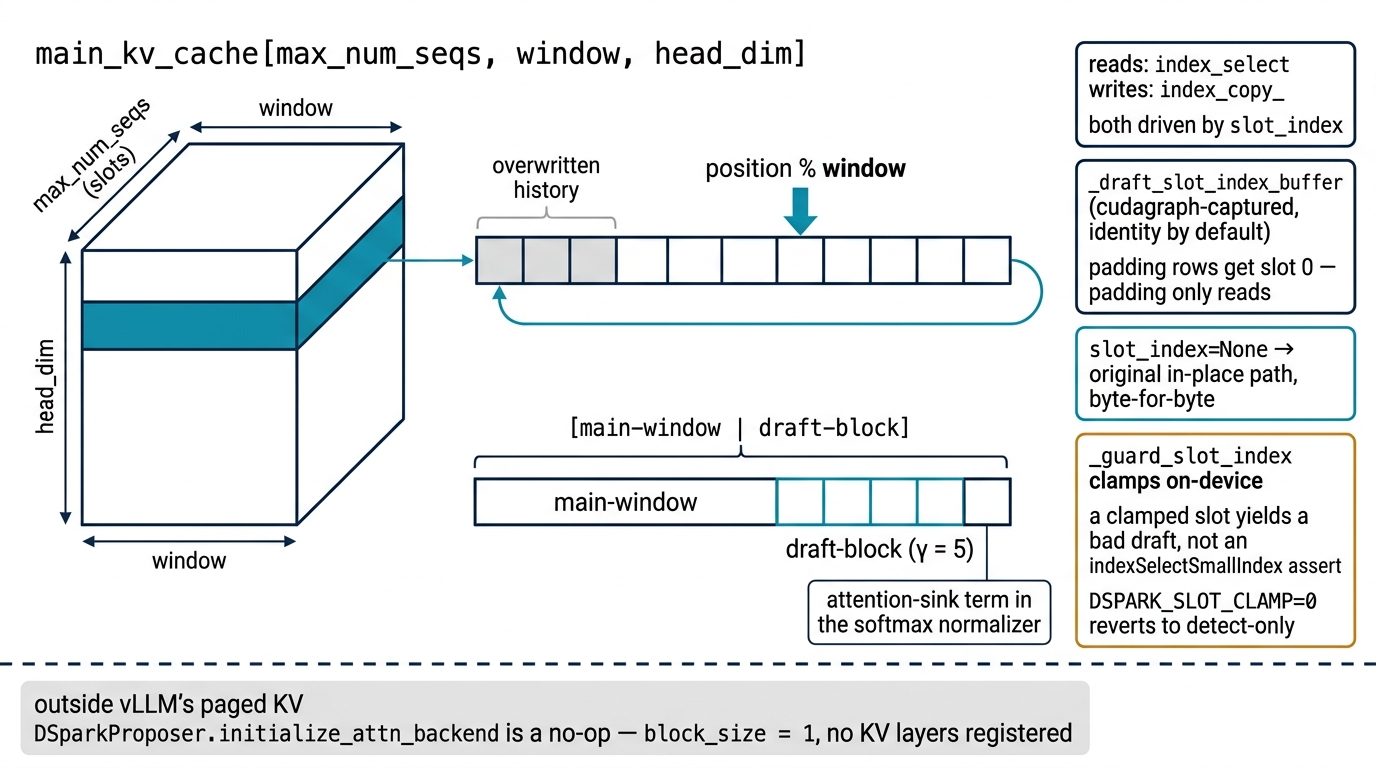
\includegraphics[width=\textwidth]{figures/ch08-drafter-kv-layout.png}
\caption{The drafter's only cross-step state. Each draft attention module
owns a persistent \code{main_kv_cache[max_num_seqs, window, head_dim]} --- a
per-request sliding window of projected target features written as a ring at
\texttt{position \% window} --- and draft attention runs over
\code{[main-window | draft-block]} with an attention-sink term in the softmax
normalizer. \code{initialize_attn_backend} is a no-op
(\code{block_size = 1}, no KV layers registered), so this sidesteps the
paged-KV allocator entirely. Reads gather and writes scatter through
\code{slot_index}; when the permutation is the identity the proposer passes
\code{slot_index=None} and the original in-place path runs byte-for-byte.}
\label{fig:specdecode-kv-layout}
\end{figure}

\section{The concurrency correctness saga}
\label{sec:specdecode-keys}

Single-stream, DSpark worked from day one. Turning up
\code{max_num_seqs} produced two distinct failures --- one silent, one loud
--- fixed by the ``Keys'' patch series
(\repofile{patches/keys-concurrency.patch}, documented as Patch~1, Patch~2,
and Patch~2b in \repofile{docs/PATCHES.md}). Together they are the best
worked example in the repository of a stateful component meeting a batch-condensing
scheduler.

\subsection{Patch 1: batch rows are not identities}

\textbf{Symptom.} At \code{max_num_seqs > 1}, draft acceptance collapsed
toward zero. Nothing crashed; the engine silently degraded to
verify-everything-reject-everything throughput.

\textbf{Root cause.} The ring buffers were indexed by \emph{batch-row
position} (\code{main_kv_cache[:batch_size]}), and the proposer carried no
request identity. vLLM v1's continuous batching \emph{condenses} the running
batch whenever a request finishes: a later request is moved into the freed
row. The model-side ring buffer row is not moved with it. After a condense,
a request reads a sliding-window history that belongs to a \emph{different}
request --- corrupted draft context, garbage drafts, acceptance collapse.
Single-stream never condenses row~0, which is exactly why the bug hid.

\textbf{Fix.} Key the state by a stable per-request slot. The proposer keeps
\code{_req_id_to_slot} and a free-slot pool: \code{_row_to_slot(req_ids)}
reclaims slots of finished requests, assigns free slots lowest-first, and
returns slots in batch-row order. The model runner threads
\code{req_ids=self.input_batch.req_ids} into \code{propose()} (a kwarg only
the DSpark proposer accepts). On the model side, \code{store_main_kv} and the
draft forward accept a \code{slot_index}: reads gather with
\code{index_select}, writes scatter with \code{index_copy_}, so the ring
follows the request id, not the row. A persistent cudagraph-captured
\code{_draft_slot_index_buffer} (identity by default) carries the slots into
the graphed draft path; padding rows get slot~0, which is safe because
padding only reads.

The elegant part is the escape hatch: when the resolved permutation is the
identity --- which a genuine single-request server always produces, since
lowest-first assignment keeps it on slot~0 --- the proposer passes
\code{slot_index=None} and the original in-place code path runs
\emph{byte-for-byte}. Warmup, capture, and single-stream serving are
provably unchanged. Gating on permutation identity rather than on
\code{batch == 1} also keeps the ``batch condensed down to one surviving
request holding a non-zero slot'' case correct.

One rule survives this whole chapter intact, and Patch~1 is where it is
written down: any state that outlives a single step must be keyed by a stable
request identity, never by a position in a batch the scheduler is free to
rearrange. The drafter's ring buffers broke that rule and degraded silently;
nothing crashed, and only acceptance recorded the damage.

\begin{figure}[htbp]
\centering
\begin{tikzpicture}[node distance=6mm and 8mm]
  % ---- LEFT: broken ----
  \node[hbtitle] (lt) {Batch-row indexing (broken)};
  \node[hbnode, below=4mm of lt, minimum width=30mm] (l0) {batch row 0: req A};
  \node[hbnode, below=3mm of l0, minimum width=30mm] (l1) {batch row 1: req B};
  \node[hbwarn, below=8mm of l1, minimum width=30mm] (lc0) {row 0: \textbf{req B}};
  \node[hblabel, align=left, right=2mm of l1.east, anchor=west] {A finishes,\\batch condenses};
  \draw[hbfail] (l1.south) -- (lc0.north);
  % ring buffers
  \node[hbhost, below=8mm of lc0, minimum width=30mm] (lr0) {ring 0: A's KV};
  \node[hbhost, below=3mm of lr0, minimum width=30mm] (lr1) {ring 1: B's KV};
  \draw[hbfail] (lc0.south) -- node[hblabel, left=1mm] {reads row 0} (lr0.north);
  \node[hblabel, below=2mm of lr1] {B drafts from A's history $\rightarrow$ acceptance $\rightarrow$ 0};
  % ---- RIGHT: fixed ----
  \node[hbtitle, right=42mm of lt] (rt) {Slot indexing (Patch 1)};
  \node[hbnode, below=4mm of rt, minimum width=34mm] (m0) {req A $\rightarrow$ slot 0};
  \node[hbnode, below=3mm of m0, minimum width=34mm] (m1) {req B $\rightarrow$ slot 1};
  \node[hbgpu, below=8mm of m1, minimum width=34mm] (rc0) {row 0: req B};
  \node[hblabel, align=left, right=2mm of m1.east, anchor=west] {condense;\\slots stable};
  \draw[hbok] (m1.south) -- (rc0.north);
  \node[hbhost, below=8mm of rc0, minimum width=34mm] (rr0) {ring 0: A's KV (freed)};
  \node[hbhost, below=3mm of rr0, minimum width=34mm] (rr1) {ring 1: B's KV};
  \draw[hbok] (rc0.east) to[out=-15,in=25]
    node[hblabel, pos=0.5, anchor=west, xshift=0.5mm, align=left, font=\tiny]
    {slot\_index\\gather} (rr1.east);
  \node[hblabel, below=2mm of rr1] {B always reads slot 1, wherever its row lands};
\end{tikzpicture}
\caption{Why acceptance collapsed under concurrency. Left: vLLM v1 condenses
the batch when request A finishes, moving request B to row 0 --- but the
drafter's persistent ring buffer stays put, so B drafts from A's
sliding-window history. Right: Patch 1 keys the ring by a stable per-request
slot; reads gather through \texttt{slot\_index}, and an identity permutation
falls back to the original in-place path byte-for-byte.}
\label{fig:specdecode-slots}
\end{figure}

\subsection{Patch 2: chunked prefill makes batches ragged}

\textbf{Symptom.} With slots fixed, realistic staggered arrivals produced
HTTP~500s:

\begin{lstlisting}
ValueError: DSpark currently requires uniform flattened per-request inputs;
got 41 rows for batch_size=2.   (dspark_proposer.py: _view_by_request)
\end{lstlisting}

\textbf{Root cause.} \code{prepare_context} reshaped the flat target hidden
states into a rectangular \code{[batch, seq, H]} view, asserting equal row
counts per request. With chunked prefill --- mandatory at long context, since
disabling it requires \code{max_num_batched_tokens >= max_model_len} --- a
single step mixes prefill and decode rows (``41 rows for batch\_size=2'' is
one request prefilling next to one decoding). The static benchmark had
passed only because all its prompts were identical length.

\textbf{Fix.} A ragged path keyed on \code{query_start_loc}: detect
non-uniform segment lengths, skip the rectangular view, compute each
request's draft anchor with a flat index
(\texttt{starts + clamp(len - rejected - 1, 0, len-1)}) and
\code{index_select} the per-request last hidden state. Storage never needed
uniformity in the first place --- it is position-addressed
(\texttt{position \% window}). A new \code{_store_main_kv_ragged} therefore
segments the flat rows, trims each segment to the window, applies the
rejected-suffix mask, and \code{index_copy_}s into each request's slot ring.
Ragged steps run eager, which is safe because mixed prefill/decode steps are
never cudagraph-captured; the uniform decode-only graphed path is untouched.
Only the \envvar{VLLM_DSPARK_GPU_REJECTED_CONTEXT_MASK=1} path was made
ragged, so serving must run with that flag set.

\subsection{Patch 2b: raggedness is not rejection}

A GSM8K quality eval --- not a benchmark --- found the last crack. A
prefill-heavy step with \emph{no} rejected tokens still crashed
(\code{got 166 rows for batch_size=3}): Patch~2 had computed \code{ragged}
only inside the branch where \code{num_rejected_tokens_gpu is not None},
but raggedness depends on \code{query_start_loc} segment lengths, not on
rejection. Fresh requests prefilling together, with nothing to reject, fell
through to the rectangular view. Patch~2b enters ragged detection whenever
the GPU-mask mode is on, regardless of the rejection tensor, defaulting
\code{rejected} to zeros when absent (\Cref{fig:specdecode-ragged-views}).
Earlier staggered tests had missed it
because their prompts were uniform-ish; GSM8K's varied prompt lengths hit it
immediately. The re-run after the fix: 200 questions at $N{=}8$ concurrency,
0 errors, 93.5\,\% accuracy vs.\ 95.0\,\% sequential, 97.5\,\% per-question
agreement --- quality-neutral within batch floating-point nondeterminism.

\begin{figure}[htbp]
\centering
\adjustbox{max width=\textwidth}{%
\begin{tikzpicture}[font=\scriptsize]
  % =================== PANEL 1 ===================
  \node[hbtitle, anchor=north west] at (0,13.90)
    {\#1 --- got 41 rows for \texttt{batch\_size=2}};

  \node[hblabel, anchor=south west, color=navy] at (0,12.92) {\texttt{query\_start\_loc}};
  \node[hblabel, anchor=south, color=navy] at (9.31,12.92) {decode};
  % flat strip of 41 rows: 40 prefill + 1 decode
  \foreach \i in {0,...,39} {
    \fill[teal!18] ({0.23*\i},12.15) rectangle ({0.23*\i+0.23},12.70);
    \draw[lightgray] ({0.23*\i},12.15) -- ({0.23*\i},12.70);
  }
  \fill[brandcyan!40] (9.20,12.15) rectangle (9.43,12.70);
  \draw[navy, thick] (0,12.15) rectangle (9.43,12.70);
  \foreach \x in {0,9.20,9.43} { \draw[navy, line width=1.1pt] (\x,12.03) -- (\x,12.82); }
  \node[anchor=center, font=\scriptsize, color=navy] at (4.60,12.425) {prefill};

  % ghosted rectangular view whose gridlines do not tile the strip
  \draw[brandgray!80, dashed] (0,11.30) rectangle (9.43,11.85);
  \draw[brandgray!80, dashed] (4.715,11.30) -- (4.715,11.85);
  \draw[clueerror!80, dashed, line width=0.8pt] (4.715,11.86) -- (4.715,12.14);
  \node[anchor=center, font=\scriptsize, color=brandgray] at (2.36,11.575)
    {\texttt{[batch, seq, H]}};

  \node[hbwarn, anchor=west, align=left, font=\scriptsize, text width=4.9cm]
        (err) at (10.40,12.10)
    {\texttt{ValueError: DSpark currently requires uniform flattened
      per-request inputs}\\[2pt]
     \texttt{dspark\_proposer.py: \_view\_by\_request}};
  \draw[hbfail] (9.55,12.42) to[out=0,in=170] (err.west);

  \node[hbfaint, anchor=north west, align=left, font=\scriptsize, text width=9.2cm,
        minimum height=0mm, inner sep=4pt] at (0,11.05)
    {the static benchmark passed --- all its prompts were the same length};

  \draw[lightgray] (0,10.30) -- (15.8,10.30);

  % =================== PANEL 2 ===================
  \node[hbtitle, anchor=north west] at (0,10.10)
    {\#2 --- got 166 rows for \texttt{batch\_size=3}};

  \draw[brandgray, thick] (0,9.00) rectangle (9.43,9.35);
  \node[hblabel, anchor=west] at (9.62,9.175) {rejection tensor: all zeros};

  % three unequal prefill segments
  \fill[teal!18] (0,8.30) rectangle (9.43,8.85);
  \draw[navy, thick] (0,8.30) rectangle (9.43,8.85);
  \foreach \x in {0,3.60,6.20,9.43} { \draw[navy, line width=1.1pt] (\x,8.18) -- (\x,8.97); }
  \node[hblabel, anchor=west, color=navy] at (9.62,8.575) {\texttt{query\_start\_loc}};

  \node[hbwarn, anchor=north west, align=left, font=\scriptsize, text width=6.0cm]
        (gate2) at (0,7.90)
    {Patch 2 computed \texttt{ragged} only inside
     \texttt{num\_rejected\_tokens\_gpu is not None}};
  \draw[hbfail] (1.80,8.16) -- (1.80,7.96);

  \draw[brandgray!80, dashed] (11.60,7.10) rectangle (15.70,7.65);
  \draw[brandgray!80, dashed] (12.97,7.10) -- (12.97,7.65);
  \draw[brandgray!80, dashed] (14.34,7.10) -- (14.34,7.65);
  \node[anchor=south, font=\scriptsize, color=brandgray] at (13.65,7.74)
    {\texttt{[batch, seq, H]}};
  \draw[hbfail] (6.42,7.40) -- (11.50,7.40);
  \node[hblabel, anchor=north west, color=clueerror] at (6.55,7.26)
    {routed back to the rectangular view};

  \node[anchor=north west, font=\scriptsize\bfseries, color=teal] at (0,6.72)
    {raggedness depends on segment lengths, not on rejection};

  \draw[lightgray] (0,6.15) -- (15.8,6.15);

  % =================== PANEL 3 ===================
  \node[hbtitle, anchor=south west, color=brandgreen!60!black] at (0,5.70) {fixed path};
  \draw[brandgreen!70!black, dashed, rounded corners=4pt] (-0.25,3.70) rectangle (15.45,5.60);

  \node[hbgpu, anchor=north west, align=left, font=\scriptsize,
        text width=2.70cm, minimum height=14mm] (s1) at (0,5.28)
    {detect non-uniform lengths from \texttt{query\_start\_loc}};
  \node[hbgpu, anchor=north west, align=left, font=\scriptsize,
        text width=2.70cm, minimum height=14mm] (s2) at (3.60,5.28)
    {\texttt{starts + clamp(len - rejected - 1, 0, len-1)}};
  \node[hbgpu, anchor=north west, align=left, font=\scriptsize,
        text width=2.70cm, minimum height=14mm] (s3) at (7.20,5.28)
    {\texttt{index\_select} the per-request last hidden state};
  \node[hbgpu, anchor=north west, align=left, font=\scriptsize,
        text width=4.60cm, minimum height=14mm] (s4) at (10.80,5.28)
    {\texttt{\_store\_main\_kv\_ragged} $\rightarrow$ trim to window
     $\rightarrow$ \texttt{index\_copy\_} into each slot ring};
  \draw[hbok] (3.12,4.58) -- (3.55,4.58);
  \draw[hbok] (6.72,4.58) -- (7.15,4.58);
  \draw[hbok] (10.32,4.58) -- (10.75,4.58);

  % =================== badges ===================
  \node[hbpatch, anchor=north west, align=left, font=\scriptsize, text width=6.6cm]
        at (0,3.30)
    {ragged steps run eager --- mixed prefill/decode steps are never
     cudagraph-captured};
  \node[hbnode, draw=navy, anchor=north west, align=left, font=\scriptsize,
        text width=7.4cm] at (7.60,3.30)
    {\texttt{VLLM\_DSPARK\_GPU\_REJECTED\_CONTEXT\_MASK=1} required};
  \node[hbgpu, anchor=north west, align=left, font=\scriptsize, text width=14.8cm]
        at (0,2.20)
    {found by GSM8K, not a benchmark --- 200 questions at N=8, 0 errors,
     93.5\,\% vs 95.0\,\%, 97.5\,\% agreement};
\end{tikzpicture}%
}
\caption{Patches 2 and 2b. \code{prepare_context} reshaped the flat target
hidden states into a rectangular \code{[batch, seq, H]} view asserting equal
rows per request, but chunked prefill mixes a prefilling request beside a
decoding one in the same step --- \code{got 41 rows for batch_size=2}.
Patch~2 added a ragged path keyed on \code{query_start_loc} but computed
raggedness only inside the branch where a rejection tensor existed, so three
fresh requests prefilling together with nothing to reject still fell through
to the rectangular view --- \code{got 166 rows for batch_size=3}. Patch~2b
decoupled the two: ragged detection runs whenever GPU-mask mode is on, with
\code{rejected} defaulting to zeros. Found by a GSM8K quality eval, not a
benchmark.}
\label{fig:specdecode-ragged-views}
\end{figure}

\begin{hbwarstory}
Before the slot map, the failure mode at long context was worse than bad
drafts: a stale row index after condensation could fire a device-side
\code{indexSelectSmallIndex} assert and kill the whole WorkerProc. The
overlay's \code{_guard_slot_index} now clamps out-of-range slots on-device
(graph-safe) and logs loudly on eager paths --- a clamped slot merely yields
a bad draft that the target rejects, instead of a dead engine. The kill
switch \envvar{DSPARK_SLOT_CLAMP=0} reverts to detect-only for A/B. The same
defensive spirit shows in the proposer's non-uniform batch guard: flattened
rows that do not divide evenly by the batch produce a one-time warning and a
skipped speculation step, never a crash.
\end{hbwarstory}

\subsection{Reproducing it: the A/B replica protocol}

\repofile{docs/SETUP.md} encodes the validation discipline: two independent
TP=2 replicas on the four Sparks, serving the \emph{same}
DeepSeek-V4-Flash-DSpark weights. Replica~A (the Rafael Caricio stack) is
the unpatched control pinned at \code{max-num-seqs=1}; replica~B (the
TonyD2Wild packaged recipe) carries the patch and sweeps
\code{max-num-seqs} 1$\to$16. Both idle at $\approx$52--54 \tokspersec{}
single-stream, so any concurrency difference is attributable to the patch,
not the packaging. The reproduction is four steps:

\begin{lstlisting}[language=bash]
git apply -p1 patches/keys-concurrency.patch   # in the overlay checkout
./build-dspark-vllm-runtime.sh                 # rebuild on every node
# .env:
#   MAX_NUM_SEQS=16
#   VLLM_DSPARK_GPU_REJECTED_CONTEXT_MASK=1    # required for the ragged path
./smoke-deepseek-v4-flash-dspark.sh            # after worker-first restart
\end{lstlisting}

\section{Acceptance in practice}
\label{sec:specdecode-acceptance}

With the drafter correct under concurrency, the question returns to the one
that justifies its existence: how much of what it drafts survives
verification --- and how to measure that without fooling yourself.

\subsection{The shape of the curve}

Per-position acceptance is the honest fingerprint of a drafter. On this
recipe the audit's expected healthy curve (\repofile{scripts/EVAL.md} and
\repofile{AUDIT.md}, verified 2026-08-16) runs from pos0
$\approx$0.93 down to pos4 $\approx$0.33 --- the ``normal DSpark collapse.''
A live TP=3 probe put concrete deltas behind it: over one measurement window,
2{,}004 accepted of 4{,}140 drafted tokens = \textbf{48.4\,\%} overall, with
the per-position curve 0.92 / 0.74 / 0.60 / 0.41 / 0.28 / 0.21. The
tokens-per-step arithmetic is worth internalizing: 4{,}140 draft tokens at
$k{=}6$ means 690 draft rounds; $2004/690 \approx 2.9$ accepted per round;
plus the guaranteed verified target token, $\approx$\textbf{3.9 tokens per
step}. That single number, multiplied by the step rate, \emph{is} the decode
throughput.

\Cref{fig:specdecode-curve} shows the $k{=}5$-vs-$k{=}6$ comparison measured
for the block-$k$ work (\Cref{sec:specdecode-choosing-k}): the 0731
checkpoint at its trained $k{=}5$ holds up much better in the tail
(pos4 0.47 vs.\ 0.23), and $k{=}6$'s sixth position accepts only 0.15 ---
drafting it costs more step time than it returns.

\subsection{Acceptance is prompt-dependent --- and probes lie}

The single most operationally important fact: acceptance on this draft head
varies enormously with the prompt (\Cref{fig:specdecode-probe-families}).
The audit-style numbered-word probes sit
at pos0 $\ge 0.90$ with a healthy curve; \emph{live natural-prose} traffic
measured pos0 0.66--0.71 and $\approx$25\,\% overall acceptance, with the
cumulative live counter around 0.78. During the September A/B campaign this
gap nearly derailed a diagnosis: a recovery gate demanded pos0 $\ge 0.85$,
and the live lane showed 0.68. Only tracing the bar back to the audit
report's ``good prompts'' curve established that 0.66--0.71 was a
pre-existing live-vs-audit gap, not a regression. The vision lane's
Prometheus snapshot tells the same story in miniature: 23.7\,\% acceptance
with positions 2--5 nearly dead (per-position accepted counts
84/63/1/1/0/0) --- natural-prose drafting, not a broken engine.

\begin{figure}[htbp]
\centering
\begin{tikzpicture}[x=1cm,y=45mm]
  % axes and gridlines
  \foreach \y/\l in {0.2/0.2, 0.4/0.4, 0.6/0.6, 0.8/0.8, 1.0/1.0} {
    \draw[hbSteel!25] (0,\y) -- (12.4,\y);
    \node[hblabel, left=1mm] at (0,\y) {\l};
  }
  \draw[thick, hbSteel] (0,0) -- (12.4,0);
  \draw[thick, hbSteel] (0,0) -- (0,1.05);
  % bars: k=5 (green), k=6 (blue); group origin 0.7 + p*2
  \foreach \p/\vfive in {0/0.93, 1/0.75, 2/0.66, 3/0.58, 4/0.47} {
    \fill[hbGreen!60] ({0.7+\p*2},0) rectangle ({1.3+\p*2},\vfive);
    \node[hblabel] at ({1.0+\p*2},{\vfive+0.045}) {\vfive};
  }
  \foreach \p/\vsix in {0/0.89, 1/0.73, 2/0.49, 3/0.34, 4/0.23, 5/0.15} {
    \fill[hbBlue!60] ({1.4+\p*2},0) rectangle ({2.0+\p*2},\vsix);
    \node[hblabel] at ({1.7+\p*2},{\vsix+0.045}) {\vsix};
  }
  % x labels
  \foreach \p in {0,1,2,3,4,5} {
    \node[hblabel] at ({1.35+\p*2},-0.06) {pos \p};
  }
  % legend
  \fill[hbGreen!60] (8.6,0.93) rectangle (9.0,0.99);
  \node[hblabel, right=1mm, anchor=west] at (9.0,0.96) {0731, $k{=}5$ (trained block)};
  \fill[hbBlue!60] (8.6,0.82) rectangle (9.0,0.88);
  \node[hblabel, right=1mm, anchor=west] at (9.0,0.85) {$k{=}6$ (divisibility-forced)};
\end{tikzpicture}
\caption{Per-position draft acceptance, \texttt{bench\_quick} on
2$\times$GB10 TP=2. At the trained block width $k{=}5$ the 0731 checkpoint
holds 0.47 acceptance at position 4; the divisibility-forced $k{=}6$ decays
to 0.23 at position 4 and only 0.15 at position 5 --- the extra noise query
costs step time for almost no accepted tokens.}
\label{fig:specdecode-curve}
\end{figure}

\begin{hblesson}
Pathological prompts lie in both directions. A repeated-word prompt
(``distributed distributed \dots'') triggers degenerate repetition that
collapses the drafter --- per-position acceptance 0.93$\to$0.33 on good
prompts vs.\ 0.72$\to$0.11 on the bad one --- and reads as a fake
$\approx$45 \tokspersec{} regression. Benchmark with unique cold prefixes and real
task instructions, quote which probe family a number came from, and never
compare a natural-prose measurement against a numbered-word bar.
The audit methodology also records abliteration draining acceptance
(0.585 vs.\ 0.718) --- watch the metric after any model swap.
\end{hblesson}

\begin{figure}[htbp]
\centering
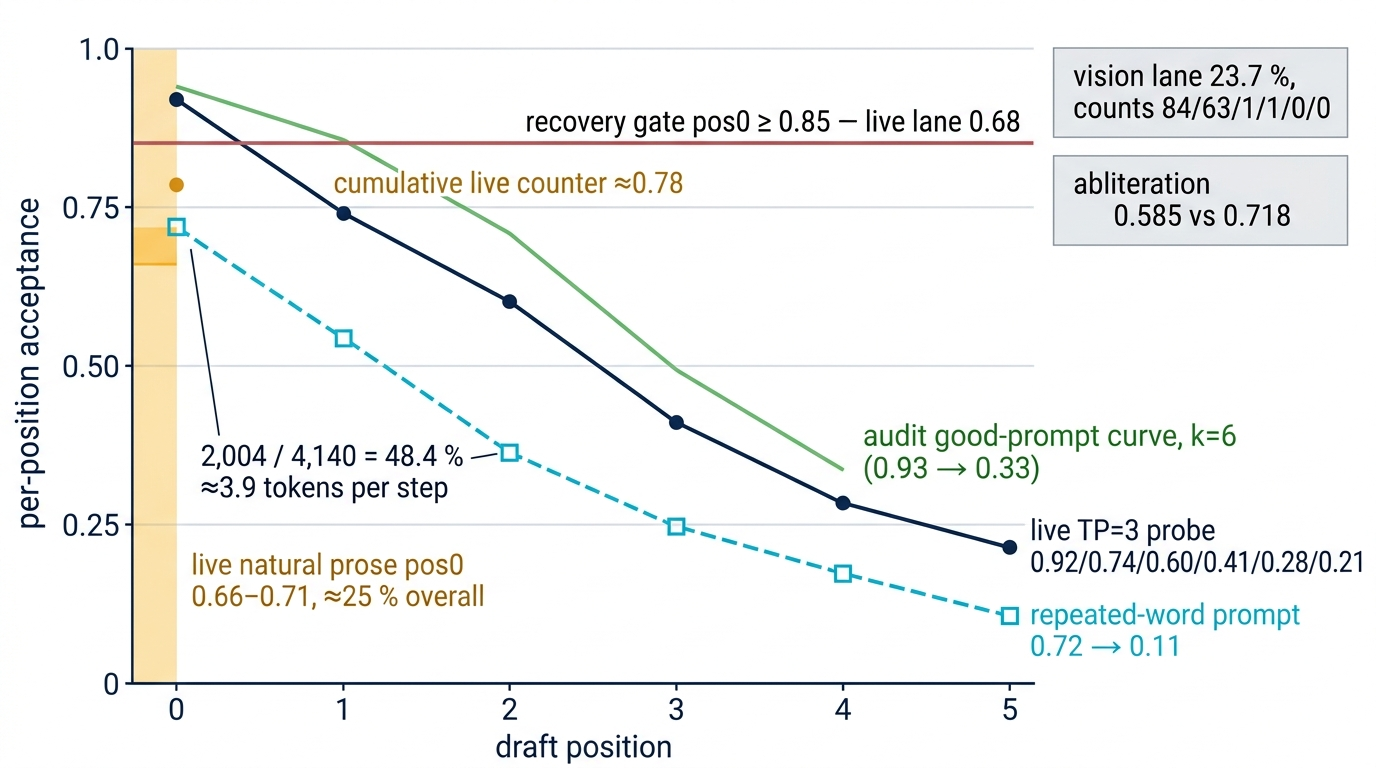
\includegraphics[width=\textwidth]{figures/ch08-acceptance-curves.png}
\caption{The same drafter, measured four ways. Audit-style numbered-word
probes hold pos0 at or above 0.90 with the normal DSpark collapse to about
0.33 by position 4; a live TP=3 probe accepted 2{,}004 of 4{,}140 drafted
tokens (48.4\,\%, $\approx$3.9 tokens per step); live natural prose sits at
pos0 0.66--0.71 with roughly 25\,\% overall against a cumulative live counter
of $\approx$0.78; and a degenerate repeated-word prompt collapses the drafter
from 0.72 to 0.11, reading as a fake $\approx$45 \tokspersec{} regression.
During the September campaign a recovery gate demanding pos0 $\ge 0.85$
failed against a live lane at 0.68 --- a pre-existing live-versus-audit gap,
not a regression. Never quote an acceptance number without its probe family.}
\label{fig:specdecode-probe-families}
\end{figure}

\subsection{Measuring it correctly}

The instrument is \repofile{scripts/spec-acceptance.py} (104 lines), run as
phase 2 of every serving audit: snapshot the
\code{vllm:spec_decode_*} counters, drive a short controlled burst, snapshot
again, and report \emph{window deltas} --- overall acceptance
$= \Delta\text{\texttt{accepted}}/\Delta\text{\texttt{drafted}}$,
per-position rate
$= \Delta\text{\texttt{per\_pos}}[i]/\Delta\text{\texttt{drafts}}$, tokens
per step
$= \Delta\text{\texttt{accepted}}/\Delta\text{\texttt{drafts}} + 1$.
Reporting the second
snapshot alone would print the container's lifetime totals, which describe
nothing about the burst just measured.

The instrument itself carries a lesson in metrics-parsing humility.

\begin{hbwarstory}
\textbf{The curve that never printed.} Until PR \ghissue{91}, the
per-position curve had \emph{never printed anything}: the parser split the
Prometheus line on \code{position=} and then on a comma, assuming another
label followed. But the pinned image emits \code{position} as the
\emph{last} label, so the parse yielded the fragment \texttt{0"\}~40263.0},
\code{int()} raised, and a bare \code{except} swallowed every position. The
fix anchors a regex directly on the \code{position} label's quoted digits,
reads \code{drafts_total} so counts become rates, and requires the
\code{_total} suffix on every counter match --- because the sibling \code{_created}
gauge carries a Unix timestamp that a naive prefix match happily reads as a
counter. The instrument now has its own regression suite
(\repofile{scripts/test-spec-acceptance.py}), including the case where spec
decode is off and the case where counters vanish between snapshots.
\end{hbwarstory}

\section{Choosing \texorpdfstring{$k$}{k}}
\label{sec:specdecode-choosing-k}

The tail of \Cref{fig:specdecode-curve} is an economic argument: a position
accepting 0.15 of its drafts adds a query row to every verify pass for
almost no accepted tokens. Acting on that argument, however, first required
deleting a rule. It is worth holding onto what $k$ actually moves: the
positions drafted, the query rows every verify pass carries, and the
CUDA-graph shapes the decode step must dispatch to --- and only the first of
those appears in an acceptance curve.

\subsection{The divisibility rule, and why DSpark is exempt}

Stock vLLM's \code{SpeculativeConfig.__post_init__} rejects any
\code{num_speculative_tokens > n_predict} not divisible by \code{n_predict}
(``Ensure divisibility for MTP module reuse''). That rule is correct for
stock MTP, which re-runs one draft layer per token. It is meaningless for
DSpark: the \code{mtp.0}--\code{mtp.2} stages are stacked into one backbone that
predicts the whole \code{dspark_block_size} block in a single pass, so the
stage count says nothing about draftable tokens. The rule's practical damage:
Vision-Exp ships \code{num_nextn_predict_layers=3} with
\code{dspark_block_size=5}, and the forced multiple-of-3 pushed the recipe to
$k{=}6$ --- one more noise query than the block was trained with. The
checkpoint's own \repofile{inference/model.py} \code{DSparkBlock} drafts
exactly $\gamma{=}5$ tokens; $k{=}5$ is the trained shape.

The unlock, \repofile{patches/hotfix-vllm-dspark-block-k.py}, is the
strictest patcher family in the repository (\Cref{ch:patches}): SHA-pinned
whole-file identity on \repofile{config/speculative.py}, pinned vLLM version
string, and a one-condition change --- \code{self.method != "dspark"}
prepended to the divisibility check. Gated by
\envvar{DSPARK_ENABLE_DSPARK_BLOCK_K=1}, paired with
\envvar{MTP_NUM_TOKENS=5}, fail-closed on any byte drift.

\begin{table}[htbp]
\centering\small
\caption{Vision-Exp, $k{=}5$ (block-$k$ unlock) vs.\ $k{=}6$
(divisibility-forced), same machine, 2026-09-03.}
\label{tab:specdecode-blockk}
\begin{tabular}{lccc}
\toprule
Metric & $k{=}5$ & $k{=}6$ & Delta \\
\midrule
Greedy decode, 8K ctx (\tokspersec{}) & 56.6 & 55.3 & $+2$\,\% \\
Greedy decode, 32K ctx (\tokspersec{}) & 56.6 & 53.6 & $+6$\,\% \\
Temp 0.6 decode (\tokspersec{}) & 49.9--56.9 & 48.6--53.1 & $+3$--$7$\,\% \\
Single-stream mini-bench (\tokspersec{}) & 56--64 & 51--55 & up to $+10$\,\% \\
Concurrency-4 aggregate (\tokspersec{}) & 110 & 106--111 & unchanged \\
TTFT & \multicolumn{2}{c}{unchanged} & --- \\
\bottomrule
\end{tabular}
\end{table}

The interpretation matters: per-position acceptance measured the same at
either $k$ (0.88 / 0.74 / 0.53 / 0.36 / 0.24), so the 2--10\,\% win is not better
drafting --- it is the cheaper step. Position 5 was accepting 0.15 of its
drafts while adding a query row to every verify pass; deleting it is nearly
pure profit at low concurrency and washes out at $c{=}4$ where the batch is
already amortizing the stream.

\subsection{The capture-size coupling}

$k$ is not a free-standing knob. The uniform decode step processes
\code{MAX_NUM_SEQS} $\times (k{+}1)$ tokens, and the CUDA-graph capture list
must include that shape, rounded up to a multiple of 8 (40 at
$6\times 6$ rows for $k{=}5$; 48 for $k{=}6$). The TP=2 lane shipped for
weeks violating exactly this coupling --- the literal boot log line was
``Truncating max\_cudagraph\_capture\_size to 40'' --- so every
full-concurrency step ran eager. \Cref{ch:perf} tells the full
predict--fix--verify arc, measured cost included. When you change $k$,
recompute the capture size; \repofile{scripts/validate-dspark-config.sh}
prints the unrounded product for exactly this reason.

Finally, the official model cards pair \code{num_speculative_tokens=7} with
\emph{greedy} draft sampling (issue \ghissue{84}). This recipe's compose
defaults to \code{probabilistic} at the trained block width, and its greedy
A/B measured a tie on this hardware. Both are legitimate operating points;
what is not legitimate is changing draft sampling and $k$ together and
attributing the delta to either alone.

\section{Tensor parallelism and the draft loop}
\label{sec:specdecode-tp}

Choosing $k$ prices the draft loop in query rows; tensor parallelism prices
the same loop in network round-trips.

\subsection{Twelve serialized collectives}

The Anemll image shards the Markov head with TP: \code{markov_w1} is a
\code{VocabParallelEmbedding} (all-reduce per lookup) and \code{markov_w2} a
\code{ParallelLMHead} whose logits route through the vocab-parallel
\code{LogitsProcessor} (all-gather). The draft block is sampled
left-to-right, so at $k{=}6$ the loop pays 2 collectives $\times$ 6 steps =
\textbf{12 serialized collectives per decode step} --- serialized because
each position's Markov bias depends on the token chosen at the previous one.
\Cref{ch:perf}'s collectives census prices the step's full collective
budget; what matters here is that the Markov dozen are the only entries in
it that cannot overlap with anything. Both Markov matrices are 66\,MB ---
replication is essentially free --- and the upstream source even carries a
\code{TODO(ben): profile ... replicate or TP-shard} comment.

\subsection{An honest negative result}

The obvious fix exists as
\repofile{patches/hotfix-dsv4-replicate-markov-head.py}:
\code{markov_w1} becomes a plain \code{nn.Embedding}, \code{markov_w2} a
\code{ReplicatedLinear}, and \code{bias()} computes locally, skipping the
\code{LogitsProcessor} all-gather entirely --- the Anemll-image equivalent
of the Stage-C overlay flag
\envvar{VLLM_DSPARK_REPLICATE_MARKOV_W1}. The
patch is correct: the A/B showed acceptance unchanged, proving the replicated
math matches the sharded math. And yet the verdict was \textbf{OFF}: no
measurable $c{=}1$ gain (the predicted 0.5--1.5\,ms is under the lane's
$\pm$10 \tokspersec{} prompt-draw noise), and the $c{=}6$ aggregate ran 122 vs.\
148 \tokspersec{} against the same-day baseline. The repository keeps the patch, its
tests, and the negative verdict side by side.

\begin{hblesson}
A first-principles estimate of 1--3\,\% is a reason to \emph{try} a patch,
not to ship it. This lane's single-stream throughput swings
$\approx$48--76 \tokspersec{} with the prompt drawn; three trials cannot resolve a
1--3\,\% knob. The campaign's rule --- eight pooled trials, same-day
baseline, host-memory gate before measuring --- exists precisely so that a
correct-but-unhelpful patch gets an honest OFF instead of a flattering
anecdote. Correctness A/Bs (acceptance unchanged) and performance A/Bs
(aggregate down) answer different questions; run both.
\end{hblesson}

\subsection{Variable-length drafting: the confidence schedulers}

The Stage-C overlay carries machinery the pinned production lane does not yet
enable: per-position confidence heads
(\code{sigmoid(proj([dense || markov_embed]))}) feeding a draft-length
scheduler behind \envvar{VLLM_DSPARK_CONFIDENCE_SCHEDULER}. The support
library (\repofile{recipe/overlay/vllm/v1/spec_decode/dspark.py}) turns
conditional per-token confidences into prefix survival probabilities and
truncates the draft \emph{non-anticipatingly} --- position $n$ admitted
using only confidences $\le n$, preserving rejection-sampling compatibility.
A hardware-aware variant scores candidate prefix schedules
against a profiled steps-per-second curve. This is the principled version of
the block-$k$ observation: position 5 at 0.15 acceptance should usually not
be drafted, and a confidence head can make that call per request per step.

Speculation stops reading as an accelerator bolted onto decode once the
weight stream is the entire cost. On this hardware the drafter \emph{is} the
decode architecture, and $k$, the ring buffers, the Markov collectives and
the CUDA-graph capture list are one coupled design rather than a knob with
side effects --- change $k$ and you change the query rows in every verify
pass and the shapes the step must dispatch to. Acceptance changed character
too: it is not a constant of the model but a joint measurement of drafter,
prompt family and instrument, which is why the same engine honestly reports
0.93 at position 0 and 0.68, and why a gate written against the wrong number
nearly manufactured a regression that was never there.

\FloatBarrier
\section*{Takeaways}

\begin{itemize}
  \item On bandwidth-bound hardware, one verify pass amortizes a
    16--17\,GB weight stream over $k{+}1$ token positions; at
    $\approx$4 accepted tokens per step this is the difference between
    $\sim$15 and the August-published 62--83 \tokspersec{} band on TP=2.
    Acceptance rate is the lever,
    and DSpark pulls it by drafting a whole $\gamma{=}5$ block in one
    non-causal pass (anchor + noise queries), sampling left-to-right through
    a rank-256 Markov bias, and keeping its only cross-step state in
    per-attention-module ring buffers \emph{outside} vLLM's paged KV.
  \item That private state is what breaks under concurrency. Any stateful
    component indexed by batch row will be corrupted by a condensing
    scheduler, so key it by request identity (Patch~1) with an
    identity-permutation fast path that keeps single-stream behavior
    byte-exact --- and remember that raggedness comes from chunked prefill,
    not from rejection: Patch~2 made the context path ragged via
    \code{query_start_loc}, and Patch~2b, found by a GSM8K eval rather than a
    benchmark, decoupled ragged detection from the rejection tensor. Run
    quality evals under concurrency; they reach code paths benchmarks never
    do.
  \item Acceptance is strongly prompt-dependent --- pos0 $\ge 0.90$ on
    numbered-word probes vs.\ 0.66--0.71 on live natural prose, with
    repeated-word prompts collapsing the drafter entirely --- so never gate
    on a number without knowing which probe family produced it. Measure it as
    counter \emph{deltas} over a controlled burst, never lifetime totals;
    anchor on \code{_total} (the \code{_created} sibling is a timestamp); and
    remember the curve that ``always printed nothing'' until PR \ghissue{91}.
    Instruments deserve regression tests.
  \item The MTP divisibility rule does not apply to stacked-stage drafters;
    running the trained block width ($k{=}5$) bought a measured 2--10\,\% by
    making the step cheaper, not the drafts better. Recompute
    \code{MAX_NUM_SEQS} $\times (k{+}1)$ capture sizes whenever $k$ changes.
  \item TP puts 12 serialized collectives inside the Markov sampling loop;
    replicating the 66\,MB head is correct but measured no win on this
    fabric --- keep honest negative results next to the patch they judge.
\end{itemize}

\chaptertransition{Acceptance multiplies the tokens a step produces, but the
step itself is priced in bytes and network round-trips --- and this chapter
kept spilling into that ledger. Twelve serialized collectives inside the
Markov loop, a capture list that must be recomputed whenever $k$ moves, a
replicated head that was provably correct and still lost throughput: none of
those verdicts can be read without the whole equation written down, stating
what a decode step must stream, what it must synchronize, and what remains
that no configuration reaches. The next chapter writes it, then spends two
one-knob-per-boot campaigns testing every lever against it. Its sharpest
result is the one nobody wanted: a third node cut the bytes each rank streams
to roughly 11.5\,GB and the model priced the step at 48\,ms --- and the
measured decode rate did not move at all.}

% =============================================================================
% Chapter 9 — Performance Engineering: A First-Principles Account
% =============================================================================

\chapter{Performance Engineering: A First-Principles Account}
\label{ch:perf}

Adding a third node to this cluster cut the bytes each rank must stream per
decode step to $\approx$11.5\,GB, and the streaming model priced the step at
$\approx$48\,ms. Yet measured single-stream decode came out at 64.3
\tokspersec{} median, no faster than the August-published two-node band of
62--83. A hardware
change that provably reduced the dominant physical cost moved the end metric
by nothing: thirteen-plus milliseconds of fixed per-step cost ate the entire
bandwidth gain. That flat number is the cleanest measurement in the repository of
what a decode step's $\approx$108 collectives and fixed software overhead
actually cost. It frames the question this chapter answers: where does
the time in a decode step \emph{have} to go, and which knobs can still move
it?

\begin{figure}[htbp]
\centering
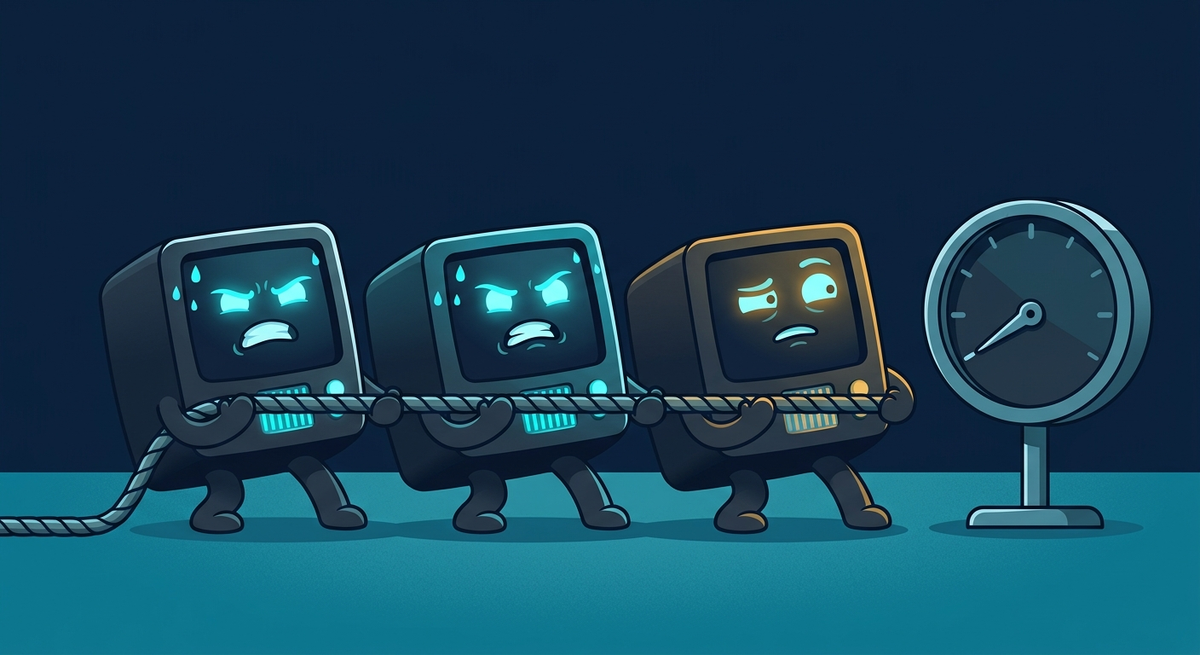
\includegraphics[width=0.80\textwidth]{figures/toon-ch09-thirdnode.png}
\caption{Everyone pulling harder; the needle unmoved. A third Spark provably cut the bytes each rank must stream per decode step to $\approx$11.5\,GB, and the streaming model priced the step at $\approx$48\,ms. Measured single-stream decode came out at 64.3 \tokspersec{} --- no faster than two nodes, because thirteen-plus milliseconds of fixed per-step cost ate the entire bandwidth gain. It is the cleanest measurement in either repository of what fixed overhead actually costs.}
\label{fig:toon-thirdnode}
\end{figure}

Every serving stack eventually accumulates a folklore of ``fast knobs'' --- flags
that someone once flipped before a good run. This repository refused to build
that folklore. Instead it built a cost model from the model's own weight shapes,
predicted where the time in a decode step must go, and then ran two disciplined
one-knob-per-boot A/B campaigns to test every prediction it could reach without
root or a kernel rebuild. The result is unusually honest: a handful of confirmed
wins, a longer list of confirmed \emph{non}-wins, one measured decline nobody
can yet explain, and a clear boundary line between what configuration can still
buy and what now requires engineering.

This chapter reconstructs that account for the inference engineer, because
the method --- model first, measure second, revert by default --- is the
transferable asset on any bandwidth-starved hardware. A cost model built from
weight shapes rules out entire classes of tuning before a single boot, and a
measurement protocol that knows its own noise floor is the only thing
standing between a verdict and an anecdote.

\section{The price of one decode step}
\label{sec:perf-costmodel}

The cost model is a subtraction. Price the bytes one step must move at the
memory bandwidth that actually exists, subtract that from the measured step
time, and whatever is left is fixed cost that no configuration knob reaches.

\subsection{Bytes per step: the streaming budget}

Start from what a single decode step at TP=2, $c=1$ must physically move. With
speculative decoding at $k=6$ (\Cref{ch:specdecode}), each step processes seven
query tokens --- one verified target token plus six draft tokens. The fable5-1
audit walked the checkpoint's shapes and produced a per-rank byte budget:

\begin{itemize}
  \item \textbf{Routed experts, $\approx$12\,GB.} Seven tokens each routing to
    top-6 of 256 experts per layer touch an expected $\approx$39 (at most 42)
    distinct experts, at 6.7\,MB per expert per rank, across 43 layers plus one
    shared expert (layers 0--2 hash-route by token id, so they pay the same
    streaming cost without a router GEMM).
  \item \textbf{Attention weights, $\approx$2.4\,GB.} The fp8 projections:
    the fused \code{fused_wqa_wkv} path, the replicated indexer projections
    (\code{wq_b}, \code{weights_proj}), and the sharded \code{wq_b},
    \code{wo_a}, \code{wo_b}.
  \item \textbf{Draft model, $\approx$0.9\,GB.} Three DSV4 MTP layers over six
    query tokens, touching $\approx$36 expert slots.
  \item \textbf{\code{lm_head}, $\approx$1.06\,GB.} The bf16
    $129{,}280 \times 4{,}096$ sharded head, read for both target and draft
    base logits.
  \item \textbf{Markov head, $\approx$0.2\,GB.} The draft's Markov \code{w2}
    read six times (33\,MB per rank per read).
\end{itemize}

The total, $\approx$16.5--17\,GB per rank per step, is the number the whole
chapter hangs on. At the DGX Spark's effective LPDDR5X bandwidth of
230--250\,GB/s that is 68--74\,ms of unavoidable weight streaming per step
(\Cref{fig:perf-bytebudget}). With $\approx$4.15 accepted tokens per step, the
streaming bound alone predicts 56--61 \tokspersec{}, against the
August-published $c=1$ band of
62--83 \tokspersec{}. The conclusion the audit drew: \textbf{roughly 80\,\% of a
$c=1$ decode step is weight streaming}, and the residual $\approx$10--15\,ms is
fixed per-step cost. No configuration knob doubles $c=1$, because no
configuration knob changes how many bytes an expert weighs.

\begin{figure}[htbp]
\centering
\adjustbox{max width=\textwidth}{%
\begin{tikzpicture}[font=\small]
  % scale: 0.72 cm per GB; segments: 12 / 2.4 / 1.06 / 0.9 / 0.2 GB
  \def\perfbh{1.0} % bar height
  % experts
  \fill[hbBlue!25]  (0,0)      rectangle (8.64,\perfbh);
  \fill[hbGreen!30] (8.64,0)   rectangle (10.37,\perfbh);
  \fill[hbAmber!35] (10.37,0)  rectangle (11.13,\perfbh);
  \fill[hbSteel!30] (11.13,0)  rectangle (11.78,\perfbh);
  \fill[hbAccent!30](11.78,0)  rectangle (11.92,\perfbh);
  \draw[hbSteel,thick] (0,0) rectangle (11.92,\perfbh);
  \draw[hbSteel!60] (8.64,0) -- (8.64,\perfbh);
  \draw[hbSteel!60] (10.37,0) -- (10.37,\perfbh);
  \draw[hbSteel!60] (11.13,0) -- (11.13,\perfbh);
  \draw[hbSteel!60] (11.78,0) -- (11.78,\perfbh);
  % in-bar labels for the big segments
  \node at (4.32,0.5)  {routed experts $\approx$12\,GB};
  \node[font=\scriptsize] at (9.5,0.5) {attn $\approx$2.4};
  % leader labels for the small segments
  \node[hblabel,anchor=west] (lh) at (12.15,-0.35) {lm\_head $\approx$1.06\,GB};
  \draw[hbSteel!70] (10.75,0) -- (12.1,-0.35);
  \node[hblabel,anchor=west] (dr) at (12.15,-0.95) {draft $\approx$0.9\,GB};
  \draw[hbSteel!70] (11.45,0) -- (12.1,-0.95);
  \node[hblabel,anchor=west] (mk) at (12.15,-1.55) {Markov w2 $\approx$0.2\,GB};
  \draw[hbSteel!70] (11.85,0) -- (12.1,-1.55);
  % total annotation
  \draw[decorate,decoration={brace,amplitude=5pt},hbBlue,thick]
    (0,\perfbh+0.15) -- (11.92,\perfbh+0.15);
  \node[hbtitle,anchor=south] at (5.96,\perfbh+0.42)
    {$\approx$16.5--17\,GB/rank/step $\;\rightarrow\;$ 68--74\,ms at 230--250\,GB/s effective};
  \node[hblabel,anchor=north west] at (0,-2.35)
    {TP=2, $c=1$, $k=6$: 7 query tokens/step (1 target + 6 draft); measured step implies
     $\approx$80\,\% streaming + 10--15\,ms fixed cost.};
\end{tikzpicture}%
}
\caption{The decode-step byte budget at TP=2, $c=1$. Expert streaming dominates:
seven query tokens route to $\approx$39 distinct experts per layer across 43
layers. At effective memory bandwidth this budget alone predicts 56--61 \tokspersec{}
at $\approx$4.15 accepted tokens/step, against the August-published
62--83 \tokspersec{} band ---
decode is $\approx$80\,\% weight-streaming-bound.}
\label{fig:perf-bytebudget}
\end{figure}

\subsection{The collectives census: $\approx$108 per step}

The fixed cost is not mysterious; the audit counted it. One TP=2 decode step
issues approximately 108 NCCL collectives (\Cref{fig:perf-collectives}):

\begin{itemize}
  \item 43 \code{wo_b} all-reduces (one per layer's output projection),
  \item 43 MoE all-reduces,
  \item 6 draft-layer all-reduces,
  \item 2 embedding all-reduces,
  \item 2 logits all-gathers --- \code{use_all_gather()} is true on CUDA, so
    every rank gathers \emph{full} logits (10.9\,MB at $c=6$),
  \item 12 serialized collectives in the Markov draft loop.
\end{itemize}

\begin{sloppypar}
The last item deserves its own sentence. The DSpark Markov head is TP-sharded
(\code{VocabParallelEmbedding} plus \code{ParallelLMHead}), and the draft
sampler runs six \emph{dependent} iterations of embed--bias--sample. Each
iteration carries one all-reduce and one all-gather of a
$[\text{num\_reqs} \times 129{,}280]$ logits tensor. The kernels live inside the
draft's CUDA graph, so there is no launch overhead --- but the network
round-trips serialize, twelve in a row, every step. At 30--50\,$\mu$s
per collective on RoCE (no GPUDirect on GB10 --- every collective bounces
through a host buffer), the census totals $\approx$3--5\,ms per step: 5--8\,\%
of a $c=1$ step, 2--3\,\% at $c=6$.
\end{sloppypar}

\begin{figure}[htbp]
\centering
\adjustbox{max width=\textwidth}{%
\begin{tikzpicture}[font=\small]
  % scale: 0.11 cm per collective; 43 + 43 + 6 + 2 + 2 + 12 = 108
  \def\colb{1.0}
  \fill[navy!30]      (0,0)     rectangle (4.73,\colb);
  \fill[navy!15]      (4.73,0)  rectangle (9.46,\colb);
  \fill[teal!32]      (9.46,0)  rectangle (10.12,\colb);
  \fill[teal!22]      (10.12,0) rectangle (10.34,\colb);
  \fill[teal!12]      (10.34,0) rectangle (10.56,\colb);
  \fill[brandcyan!45] (10.56,0) rectangle (11.88,\colb);
  \draw[brandgray,thick] (0,0) rectangle (11.88,\colb);
  \foreach \x in {4.73,9.46,10.12,10.34,10.56} {
    \draw[brandgray!60] (\x,0) -- (\x,\colb);
  }
  \draw[brandcyan!70!black,very thick] (10.56,0) rectangle (11.88,\colb);
  % in-bar labels for the two 43-wide segments
  \node[align=center] at (2.365,0.5) {\textbf{43}\\\texttt{wo\_b} all-reduces};
  \node[align=center] at (7.095,0.5) {\textbf{43}\\MoE all-reduces};
  % total
  \node[hbtitle,anchor=south west] at (0,1.15)
    {$\approx$108 collectives per TP=2 decode step};
  % fan of leader labels for the narrow segments
  \node[hblabel,anchor=west] at (12.15,3.20) {\textbf{6} draft-layer all-reduces};
  \draw[brandgray!70] (9.79,\colb) -- (12.10,3.20);
  \node[hblabel,anchor=west] at (12.15,2.55) {\textbf{2} embedding all-reduces};
  \draw[brandgray!70] (10.23,\colb) -- (12.10,2.55);
  \node[hblabel,anchor=west] at (12.15,1.90) {\textbf{2} logits all-gathers};
  \draw[brandgray!70] (10.45,\colb) -- (12.10,1.90);
  \node[hblabel,anchor=west,color=brandcyan!70!black] at (12.15,1.25)
    {\textbf{12} Markov loop};
  \draw[brandcyan!70!black] (11.22,\colb) -- (12.10,1.25);
  \node[hbfaint,anchor=north west,align=left,font=\scriptsize,text width=41mm]
    at (12.15,0.95)
    {\texttt{use\_all\_gather()} true on CUDA --- full logits, 10.9\,MB at $c=6$\\[2pt]
     \texttt{VocabParallelEmbedding} / \texttt{ParallelLMHead}};
  % pull the serialized dozen down into a sequence strip
  \draw[brandcyan!70!black,dashed] (10.56,0) -- (0,-1.45);
  % right leader dropped down the near side of the note box, then across below it
  \draw[brandcyan!70!black,dashed] (11.88,0) -- (12.00,-1.05) -- (16.20,-1.45);
  % cells sized to the label they hold, with clear space on both sides
  \foreach \i in {0,1,2,3,4,5} {
    \fill[ice] ({\i*2.70},-2.25) rectangle ({\i*2.70+2.70},-1.45);
    \draw[brandgray!45] ({\i*2.70+0.90},-2.25) -- ({\i*2.70+0.90},-1.45);
    \draw[brandgray!45] ({\i*2.70+1.62},-2.25) -- ({\i*2.70+1.62},-1.45);
    \draw[brandcyan!70!black,thick] ({\i*2.70},-2.25) rectangle ({\i*2.70+2.70},-1.45);
    \node[font=\tiny,anchor=base] at ({\i*2.70+0.45},-1.90) {embed};
    \node[font=\tiny,anchor=base] at ({\i*2.70+1.26},-1.90) {bias};
    \node[font=\tiny,anchor=base] at ({\i*2.70+2.16},-1.90) {sample};
  }
  \node[hblabel,anchor=north] at (8.1,-2.40)
    {each of six dependent iterations: 1 all-reduce $+$ 1 all-gather
     $[\text{num\_reqs} \times 129{,}280]$};
  \node[hbpatch,anchor=north,align=center,font=\scriptsize,text width=126mm]
    at (8.1,-2.90)
    {serialized --- each position's Markov bias depends on the token chosen
     at the previous one};
  \node[hblabel,anchor=north] at (8.1,-3.95)
    {kernels live inside the draft's CUDA graph --- no launch overhead;
     the network round-trips serialize};
  % pricing footer
  \draw[brandgray!50] (0,-4.65) -- (16.35,-4.65);
  \node[hblabel,anchor=north west] at (0,-4.85)
    {30--50\,$\mu$s per collective on RoCE};
  \draw[brandgray!40] (4.60,-4.75) -- (4.60,-5.20);
  \node[hblabel,anchor=north west] at (4.80,-4.85) {no GPUDirect on GB10};
  \draw[brandgray!40] (8.30,-4.75) -- (8.30,-5.20);
  \node[hblabel,anchor=north west] at (8.50,-4.85)
    {$\approx$3--5\,ms per step $=$ 5--8\,\% of a $c=1$ step, 2--3\,\% at $c=6$};
  % closing row: cost-model chip and the TP=3 annotation
  \node[hbbox,anchor=north west,align=left,font=\scriptsize,text width=64mm]
    at (0,-5.40)
    {bytes (68--74\,ms) $+$ fixed cost (10--15\,ms) $=$ the step};
  \node[hbpatch,anchor=north west,align=left,font=\scriptsize,text width=74mm]
    at (8.50,-5.40)
    {\textbf{TP=3: $\approx$11.5\,GB/rank, $\approx$48\,ms predicted,
     64.3 \tokspersec{} measured}\\[2pt]
     three-rank ring $\approx2\times$ the latency; heads padded $64 \to 72$;
     ring spans two physical links};
\end{tikzpicture}%
}
\caption{The other half of the cost model. One TP=2 decode step issues
approximately 108 NCCL collectives --- 43 \code{wo_b} all-reduces, 43 MoE
all-reduces, 6 draft-layer all-reduces, 2 embedding all-reduces, 2
full-logits all-gathers (10.9\,MB at $c=6$, since \code{use_all_gather()} is
true on CUDA), and the 12 in the Markov draft loop. At 30--50\,$\mu$s per
collective on RoCE --- with no GPUDirect on GB10, so every collective bounces
through a host buffer --- that is roughly 3--5\,ms per step, 5--8\,\% of a
$c=1$ step. The Markov dozen are the only entries that cannot overlap: six
dependent iterations of embed--bias--sample, each carrying one all-reduce and
one all-gather, serialized because each position's bias depends on the
previous token. This fixed cost is what made TP=3's drop to $\approx$11.5\,GB
per rank --- priced at $\approx$48\,ms --- arrive as 64.3 \tokspersec{}, no
faster than two nodes.}
\label{fig:perf-collectives}
\end{figure}

\subsection{The TP=3 natural experiment}

The strongest evidence that fixed cost, not bandwidth, now governs $c=1$
came free of charge --- it is the flat TP=3 result the chapter opened with.
At audit time the cluster happened to be running the three-node TP=3
experiment (\Cref{ch:scaling}). The mechanism behind the flat number is
exactly the fixed cost this section has been counting: a three-rank ring has
roughly twice the latency of a two-rank exchange, the attention heads are
padded $64 \to 72$ to divide by three, and the ring spans two different
physical links. As the opening showed, that fixed cost ate the entire
bandwidth gain the streaming model had priced in. TP=3 is a capacity win
(5.0\,M KV tokens, 16 slots, $4.79\times$ concurrency at 1M) --- it is not a
latency win, and the cost model says it cannot be until the fixed per-step
costs shrink.

\begin{hblesson}
When a hardware upgrade that provably reduces the dominant physical cost
(bytes per rank) fails to move the end metric, you have measured your fixed
overhead more convincingly than any profiler would. The TP=3 boot was run for
capacity; its flat $c=1$ number is the cleanest single measurement in the repository
of what the $\approx$108 collectives and eager launches cost.
\end{hblesson}

\section{Where throughput actually comes from}
\label{sec:perf-throughput}

The decode side has exactly two multipliers, and both work the same way:
spreading one weight stream over more tokens. Concurrency supplies those
tokens from other requests, speculative acceptance from the same one.
Prefill, as the last part of this section shows, obeys different economics
entirely.

\subsection{Concurrency amortizes the weight stream}

If one step must stream 16.5\,GB regardless, the obvious move is to make each
step serve more tokens. The same expert weights read once serve every sequence
in the batch, so aggregate throughput climbs steeply with concurrency while
per-stream rates fall gently. The published 1~August sweep at 256-token prompts
shows the curve exactly (\Cref{fig:perf-concurrency}): aggregate 69.1 \tokspersec{} at
$c=1$, 104.9 at $c=2$, 164.5 at $c=4$, 191.2 at $c=6$ --- while per-stream
decode declines 75.4 $\to$ 58.3 $\to$ 46.8 $\to$ 36.9 \tokspersec{}. Six concurrent
chats buy roughly $2.8\times$ the fleet throughput of one on that sweep (the
audit quotes $\approx$$2.2\times$ against its own published TP=2 reference
band), because the marginal sequences ride a weight stream that was being paid
for anyway.

\begin{figure}[htbp]
\centering
\begin{tikzpicture}[font=\small]
  % x: concurrency 0..6.8 at 1.5cm/unit ; y: tok/s 0..200 at 0.026 cm per tok/s
  \def\perfX#1{#1*1.5}
  \def\perfY#1{#1*0.026}
  % grid
  \foreach \y in {50,100,150,200} {
    \draw[hbSteel!25] (0,\perfY{\y}) -- (\perfX{6.8},\perfY{\y});
    \node[hblabel,anchor=east] at (-0.1,\perfY{\y}) {\y};
  }
  \draw[hbarrow] (0,0) -- (\perfX{7.1},0) node[hblabel,anchor=north west,yshift=-1mm] {concurrency $c$};
  \draw[hbarrow] (0,0) -- (0,\perfY{210}) node[hblabel,anchor=south] {\tokspersec{}};
  \foreach \c in {1,2,4,6} {
    \draw[hbSteel] (\perfX{\c},0) -- (\perfX{\c},-0.08);
    \node[hblabel,anchor=north] at (\perfX{\c},-0.1) {\c};
  }
  % aggregate line
  \draw[hbflow,very thick]
    (\perfX{1},\perfY{69.1}) -- (\perfX{2},\perfY{104.9}) -- (\perfX{4},\perfY{164.5}) -- (\perfX{6},\perfY{191.2});
  \foreach \c/\v in {1/69.1,2/104.9,4/164.5,6/191.2} {
    \fill[hbBlue] (\perfX{\c},\perfY{\v}) circle (2pt);
    \node[hblabel,color=hbBlue,anchor=north west] at (\perfX{\c}+0.08,\perfY{\v}-0.06) {\v};
  }
  \node[hbtitle,anchor=west] at (\perfX{4.35},\perfY{188}) {aggregate};
  % per-stream line
  \draw[color=brandgreen!70!black,very thick,dashed]
    (\perfX{1},\perfY{75.4}) -- (\perfX{2},\perfY{58.3}) -- (\perfX{4},\perfY{46.8}) -- (\perfX{6},\perfY{36.9});
  \foreach \c/\v in {1/75.4,2/58.3,4/46.8,6/36.9} {
    \fill[hbGreen!70!black] (\perfX{\c},\perfY{\v}) circle (2pt);
  }
  \node[hblabel,color=hbGreen!60!black,anchor=north west] at (\perfX{4.15},\perfY{31}) {per-stream};
\end{tikzpicture}
\caption{Aggregate and per-stream decode \tokspersec{} versus concurrency, 256-token
prompts, natural completions (published 1~August 2026 sweep). Aggregate climbs
$69.1 \to 191.2$ \tokspersec{} from $c=1$ to $c=6$ --- roughly $2.8\times$ on this
sweep, against the audit's $\approx$$2.2\times$ rule of thumb for the published
TP=2 band --- because concurrent sequences amortize the same 16.5\,GB/step
weight stream; per-stream rates decline gently from 75.4 to 36.9 \tokspersec{}.}
\label{fig:perf-concurrency}
\end{figure}

\subsection{Acceptance is the other multiplier}

The second throughput lever divides rather than multiplies: bytes per
\emph{accepted} token, since every accepted draft token is a token generated
without another 16.5\,GB step. Acceptance is strongly prompt-dependent on
this draft head --- roughly half the drafted tokens accepted on
numbered-word probes versus a quarter on live natural prose --- and that gap,
not any \repofile{.env} knob, is the largest remaining decode lever
(\Cref{sec:perf-remains}). The mechanism, the curves, and the probe
discipline are \Cref{ch:specdecode}'s subject.

\subsection{Prefill obeys different economics}

Decode is bandwidth-bound; prefill is compute- and kernel-bound, and at long
context one component dominates everything: the Lightning indexer. The indexer
is \emph{replicated} across TP ranks (\code{wq_b} and \code{weights_proj} are
\code{ReplicatedLinear} --- the source comments ``no tensor parallel, just
replicated''), so every rank scores all 64 index heads against the entire
compressed key range. The work is $O(\text{queries} \times \text{keys})$: at
900K context each 1{,}024-token chunk costs $\approx$80\,TFLOP of scoring,
$\approx$0.8\,s of tensor-core time, \emph{duplicated on both GPUs}. That
quadratic term is why prefill falls from 2{,}563 \tokspersec{} at 2K context to
$\approx$875 \tokspersec{} on the 900K acceptance run (899{,}994 prompt tokens,
1{,}028.85\,s TTFT).

The MoE path compounds it at short and medium context:
b12x runs W4A16 (dequantize to bf16) for the checkpoint's
\code{fp4_e8m0_k32} expert format because its NVFP4 tensor-core path accepts
only modelopt-format weights. The largest prefill FLOP consumer therefore
runs at roughly a quarter of the hardware's FP4$\times$FP8 rate. Streaming,
collectives, replicated indexer scoring, dequantized MoE: each of these
costs is attackable at a very different price, and ranking those prices is
what the audit did next.

\section{Ten findings, ranked by expected value over effort}
\label{sec:perf-findings}

The audit distilled everything above into ten ranked findings
(\Cref{tab:perf-findings}). The ranking discipline matters as much as the
content: each row states a mechanism, an evidence trail, an \emph{expected}
effect with an honest error bar, and the effort class --- host command, one
compose line, a $\sim$60-line patch, or multi-day kernel work. Findings are
predictions until measured; \Cref{sec:perf-ab} is where several of them met
reality.

\begin{table}[htbp]
\centering
\small
\caption{The fable5-1 audit's ten findings, ranked by expected value over
effort (condensed from the 2026-09-02 report).}
\label{tab:perf-findings}
\begin{tabular}{@{}cl>{\raggedright\arraybackslash}p{5.2cm}>{\raggedright\arraybackslash}p{3.4cm}>{\raggedright\arraybackslash}p{2.5cm}@{}}
\toprule
\# & Class & Finding & Expected effect & Effort \\
\midrule
1 & stability & Host memory exhausted at boot on both nodes (\code{NV_ERR_NO_MEMORY}; worker swap 10.4\,GB, polkitd leak 3.1\,GB; KV pool sized from the worst rank) & reclaim 5--8\,GB $\to$ util $0.83 \to 0.86$--$0.88$ = +20--35\,\% KV tokens & host-side + restart \\
2 & config & $c=6$ decode shape (42 tokens) not CUDA-graph captured: argv 42 truncated to 40, rounded to multiples of 7 $\to$ graphs [7,14,21,28,35]; $c=6$ runs eager & +3--10\,\% $c=6$ aggregate & one compose line \\
3 & fabric & NCCL pinned to one CX7 PCIe function (Gen5 $\times$4 $\approx$ 126\,Gb/s feeding a 200\,Gb/s port); RoCE MTU 1024; duplicate subnet on the second PF & prefill comm up to $\sim$2$\times$; decode unchanged & host + env \\
4 & patch & Markov head TP-sharded $\to$ 12 serialized collectives/step; both matrices 66\,MB, replication free & $-$12 collectives $\approx$ 0.5--1.5\,ms (1--3\,\%) & $\sim$60-line patch \\
5 & kernel & W4A16 everywhere: no MXFP4 tensor-core MoE for \code{fp4_e8m0_k32}; \envvar{B12X_W4A16_TC_DECODE} untested and not plumbed through compose & TC-decode 0--10\,\% $c=1$ (A/B); MXFP4 MoE $\to$ prefill +30--60\,\% & env now; kernels later \\
6 & engineering & Lightning indexer replicated across ranks; dominates prefill at $\geq$128K & sequence-parallel indexer $\to$ up to $\sim$1.8$\times$ long-context prefill & multi-day \\
7 & patch & Static 1024-token prefill chunk cap even with no decode lanes active & $c=1$ TTFT $-$10--25\,\% on $\leq$32K prompts & $\sim$30-line patch \\
8 & upstream & \code{nvfp4_ds_mla} is byte-identical to \code{fp8_ds_mla} (584\,B/row) --- no 4-bit KV today & true NVFP4 row $\to$ +50\,\% KV tokens & FlashInfer SM120 work \\
9 & fairness & Live \envvar{DSPARK_MAX_INFLIGHT_PREFILLS}=2 despite the \ghissue{154} revert to 1 & decide explicitly (fairness vs the 32K$\times$c4 floor) & \repofile{.env} + restart \\
10 & latency & Warmup gaps: sparse-MLA autotune covers only tokens=16; CuTeDSL warmup skipped; first requests JIT mid-serve & removes first-request cliffs; closes the JIT-vs-watchdog hazard (\ghissue{117}) & scripts + restart \\
\bottomrule
\end{tabular}
\end{table}

Finding \#1, the top-ranked row, deserves a trace of its own, because its
punchline is structural. During the audited boot, both nodes' kernel logs
recorded repeated \code{NVRM: Out of memory [NV_ERR_NO_MEMORY]} allocation
failures in the profile/autotune/capture window --- the boot survived only
because the failing allocations were retried elsewhere. The worker was the
worse host: 5.4\,GB MemAvailable, 10.4\,GB of swap in use, and a
\code{polkitd} process holding 3.1\,GB of RSS (a known polkit leak under
GNOME). The node was still on \code{graphical.target}, with Xorg and
gnome-shell holding GPU contexts.

The consequence reaches past one machine:
the worker's KV pool came out 1.19\,GiB below the head's (33.82 versus
35.01\,GiB), and vLLM sizes the shared pool from the \emph{worst} rank.
One leaky daemon on one node thus taxed the whole cluster's KV capacity. That
chain --- host bloat, worst-rank sizing, fleet-wide KV loss --- is what
drives the host-memory gate of \Cref{sec:perf-ab}, the unified-memory
warning below it, and the root-only hunt of \Cref{sec:perf-remains}.

Finding \#2 is worth tracing in full because it became the book's cleanest
predict--fix--verify arc. The compose file computes the CUDA-graph capture size
as \code{MAX_NUM_SEQS} $\times$ (\code{MTP_NUM_TOKENS}$+1$) $= 42$. vLLM's
default capture list is $[1,2,4,8,16,24,32,40]$, and 42 is not on the stride.
The boot log therefore prints, verbatim, \code{Truncating max_cudagraph_capture_size to
40}, and spec-decode rounding then yields FULL graphs at $[7,14,21,28,35]$
only. A six-request decode step is exactly 42 tokens --- it dispatches to
\emph{no} graph and runs fully eager, issuing 1{,}500--1{,}800 Python-launched
kernels (\Cref{fig:perf-captureladder}).

\begin{hbnote}
The trace also exhumed a perfect measurement parable. An earlier
(19~August) A/B had concluded ``no $c=6$ lift'' --- but it ran at $k=5$ with
a capture cap of 32, whose $c=6$ shape (36 tokens) was \emph{also}
uncaptured in both arms. Both arms ran the untested configuration; the
experiment never tested the question. Gates before numbers exist precisely
because a clean-looking A/B can be null by construction.
\end{hbnote}

The fix is one line of compose arithmetic:

\begin{lstlisting}[language=bash]
# docker-compose.dspark.yml: round the capture size up to a multiple of 8
--max-cudagraph-capture-size $(( (MAX_NUM_SEQS*(MTP_NUM_TOKENS+1)+7)/8*8 ))
# 6*(6+1)=42 -> 48; boot gate: no "Truncating", "Capturing CUDA graphs (FULL) 6/6"
\end{lstlisting}

\begin{figure}[htbp]
\centering
\adjustbox{max width=\textwidth}{%
\begin{tikzpicture}[font=\small]
  % one shared token-count scale: x = 3.0 + 0.2*tokens, 0..48
  % ---------- row 1: vLLM's default capture list ----------
  \node[anchor=east,align=right,font=\scriptsize,text width=33mm] at (2.70,0)
    {\textbf{vLLM default capture list}\\\texttt{[1,2,4,8,16,24,32,40]}};
  \draw[navy,thick] (3.0,0) -- (12.6,0);
  \foreach \t in {1,2,4,8,16,24,32,40} {
    \draw[navy] ({3.0+0.2*\t},0) -- ({3.0+0.2*\t},-0.12);
    \node[font=\tiny,anchor=north,color=navy] at ({3.0+0.2*\t},-0.14) {\t};
  }
  \draw[clueerror,thick] (11.28,-0.12) -- (11.52,0.12);
  \draw[clueerror,thick] (11.28,0.12)  -- (11.52,-0.12);
  \node[hblabel,color=clueerror,anchor=south east] at (11.20,0.10)
    {42 is not on the stride};
  % ---------- row 2: after truncation ----------
  \node[anchor=east,align=right,font=\scriptsize,text width=33mm] at (2.70,-2.0)
    {\textbf{after truncation}\\\texttt{[7,14,21,28,35] FULL}};
  \node[anchor=west,font=\scriptsize\ttfamily,color=clueerror] at (3.0,-1.42)
    {Truncating max\_cudagraph\_capture\_size to 40};
  \fill[amber!25] (10.0,-2.25) rectangle (11.4,-1.75);
  \draw[navy,thick] (3.0,-2.0) -- (12.6,-2.0);
  \foreach \t in {7,14,21,28,35} {
    \draw[navy] ({3.0+0.2*\t},-2.0) -- ({3.0+0.2*\t},-2.12);
    \node[font=\tiny,anchor=north,color=navy] at ({3.0+0.2*\t},-2.14) {\t};
  }
  % the shape that falls in the gap
  \draw[brandcyan!70!black,line width=1.2pt] (11.4,-2.48) -- (11.4,-1.36);
  \node[anchor=south east,font=\scriptsize,color=brandcyan!70!black] at (12.6,-1.32)
    {42 tokens $=$ $6 \times (k{=}6 + 1)$};
  \node[hbgpu,anchor=north west,align=left,font=\scriptsize,text width=38mm]
    (rcproof) at (12.9,0.55)
    {\textbf{proven by reversal}\\[2pt]
     sequence 2 booted the old expression as \texttt{capture42}\\[2pt]
     $c=6$ aggregate $139 \to 122$ --- a 12\,\% loss, all trials below the
     baseline minimum\\[2pt]
     boot log: \texttt{FULL 5/5}};
  \node[hbwarn,anchor=north west,align=left,font=\scriptsize,text width=38mm]
    (rceager) at ([yshift=-3mm]rcproof.south west)
    {dispatches to \textbf{no graph}\\runs \textbf{fully eager}\\
     1{,}500--1{,}800 Python-launched kernels};
  \draw[hbarrow,color=brandcyan!70!black] (11.5,-2.48) to[out=-15,in=190] (rceager.west);
  % ---------- row 3: after the fix ----------
  \node[anchor=east,align=right,font=\scriptsize,text width=33mm] at (2.70,-4.0)
    {\textbf{after the fix}\\\texttt{6*(6+1)=42 -> 48}};
  \node[anchor=west,align=left,font=\scriptsize\ttfamily,
        color=brandgreen!55!black] at (3.0,-3.40)
    {-{}-max-cudagraph-capture-size\\
     \$(( (MAX\_NUM\_SEQS*(MTP\_NUM\_TOKENS+1)+7)/8*8 ))};
  \draw[brandgreen!60!black,thick] (3.0,-4.0) -- (12.6,-4.0);
  \foreach \t in {7,14,21,28,35} {
    \draw[brandgreen!60!black] ({3.0+0.2*\t},-4.0) -- ({3.0+0.2*\t},-4.12);
    \node[font=\tiny,anchor=north,color=brandgreen!55!black] at ({3.0+0.2*\t},-4.14) {\t};
  }
  \draw[brandgreen!60!black,line width=1.2pt] (11.4,-4.20) -- (11.4,-3.80);
  \node[font=\tiny,anchor=north,color=brandgreen!55!black] at (11.4,-4.22) {42};
  \draw[brandgreen!60!black] (12.6,-4.12) -- (12.6,-3.88);
  \node[font=\tiny,anchor=north,color=brandgreen!55!black] at (12.6,-4.14) {48};
  \node[hbgpu,anchor=north west,align=left,font=\scriptsize,text width=38mm]
    (rcfixed) at ([yshift=-3mm]rceager.south west)
    {no \texttt{Truncating}\\\texttt{Capturing CUDA graphs (FULL) 6/6}};
  % ---------- right column: the proof and the parable ----------
  \node[hbpatch,anchor=north west,align=left,font=\scriptsize,text width=38mm]
    (rcaug) at ([yshift=-3mm]rcfixed.south west)
    {\textbf{19 August}\\[2pt]
     both arms ran $k=5$ with a cap of 32\\[2pt]
     $c=6$ shape 36 tokens --- also uncaptured in both arms\\[2pt]
     the experiment never tested the question};
  % ---------- coupling note ----------
  \node[hbfaint,anchor=north west,align=left,font=\scriptsize,text width=88mm]
    at (0,-4.95)
    {\texttt{scripts/validate-dspark-config.sh} prints the unrounded
     \texttt{MAX\_NUM\_SEQS} $\times$ (\texttt{MTP\_NUM\_TOKENS+1})};
\end{tikzpicture}%
}
\caption{Finding \#2, the book's cleanest predict--fix--verify arc. The
compose file computed the capture size as \code{MAX_NUM_SEQS} $\times$
(\code{MTP_NUM_TOKENS}${}+1$) $= 42$, but 42 is not on vLLM's default capture
stride $[1,2,4,8,16,24,32,40]$, so the boot printed
\code{Truncating max_cudagraph_capture_size to 40} and spec-decode rounding
left FULL graphs at $[7,14,21,28,35]$ only --- leaving the exact 42-token
six-request decode step in the gap, dispatching to no graph and issuing
1{,}500--1{,}800 Python-launched kernels per step. Rounding the expression up
to a multiple of 8 yields 48 and closes the gap; sequence 2 proved it by
reversal, booting the old expression as \code{capture42} and watching $c=6$
aggregate fall from 139 to 122. The 19~August A/B that found ``no $c=6$
lift'' had run both arms at $k=5$ with a cap of 32, whose $c=6$ shape was
also uncaptured --- a clean-looking experiment that was null by
construction.}
\label{fig:perf-captureladder}
\end{figure}

\section{The A/B campaigns as methodology}
\label{sec:perf-ab}

The protocol below is shaped by one property of this lane: a single $c=1$
trial can land anywhere in a $\pm$10 \tokspersec{} band on an unchanged boot,
which is wide enough to manufacture almost any verdict. One knob per boot,
gates before numbers, and eight pooled trials are all consequences of
refusing to measure through that noise.

\subsection{One knob, one boot, gates before numbers}

Two campaigns (2026-09-02, sequences 1 and 2) turned the findings into
verdicts. The two drivers, \repofile{scripts/ab-measure.sh} and
\repofile{scripts/ab-boot.sh}, enforce a fixed pipeline per knob
(\Cref{fig:perf-abflow}). Edit exactly one line of \repofile{.env.dspark};
stop and start the whole stack (a fresh boot per variable --- container
restarts do not re-render compose); then pass \emph{boot gates on both ranks}
before any measurement: the expected \code{[dspark-...] patched} lines, FULL
graphs 6/6 with no truncation, the DeepGEMM sm121 alias applied $\times$4, zero
\code{EngineDead} or NCCL warnings.

Next a \emph{host-memory gate}: a boot that
lands below the MemAvailable threshold is not measured at all, because numbers
taken on a swapping host are not trustworthy. Only then does the measurement
battery run: pooled $c=1$ decode trials, $c=2$, $c=6$ aggregate, TTFT at
8K/32K/128K, natural-prose and numbered-word acceptance, and (in sequence 2) a
purpose-built fairness driver, \repofile{scripts/ab-fairness.py}, that measures
the per-stream TTFT and decode spread of a $c=4$ 8K case.

\begin{figure}[htbp]
\centering
\adjustbox{max width=\textwidth}{%
\begin{tikzpicture}[node distance=9mm and 5mm,font=\scriptsize]
  \node[hbnode] (edit) {Edit \texttt{.env.dspark}\\\emph{one} knob};
  \node[hbnode,right=of edit] (boot) {\texttt{stop} + \texttt{start}\\fresh boot};
  \node[hbnode,right=of boot] (gates) {Boot gates, both ranks:\\patched lines, FULL 6/6,\\no truncation, alias $\times$4};
  \node[hbnode,right=of gates] (mem) {Host-memory gate\\MemAvailable $\geq$ gate};
  \node[hbnode,below=of mem] (meas) {Measure: 8$\times$ c=1 pooled,\\c=2, c=6, TTFT 8/32/128K,\\acceptance, fairness c=4};
  \node[hbbox,left=of meas] (verdict) {Verdict};
  \node[hbgpu,below=7mm of verdict,xshift=-22mm] (keep) {KEEP: target metric\\beyond noise band,\\nothing else worse};
  \node[hbwarn,below=7mm of verdict,xshift=22mm] (revert) {REVERT: tie, any\\regression, or gate\\failure (unmeasured)};
  \draw[hbflow] (edit) -- (boot);
  \draw[hbflow] (boot) -- (gates);
  \draw[hbflow] (gates) -- (mem);
  \draw[hbflow] (mem) -- (meas);
  \draw[hbflow] (meas) -- (verdict);
  \draw[hbok] (verdict) -- (keep);
  \draw[hbfail] (verdict) -- (revert);
  % routed clear of the Measure box: bulge to the right of it, then in from the right
  \draw[hbfail] ([xshift=3mm]mem.south east) to[out=0,in=0,looseness=1.6]
    node[hblabel,pos=0.10,anchor=west,xshift=2mm,align=left]
    {below gate:\\skip measurement} (revert.east);
\end{tikzpicture}%
}
\caption{The A/B pipeline enforced by \repofile{scripts/ab-boot.sh}: one env
edit per boot, boot gates on both ranks before any number is taken, a
host-memory gate that skips (rather than pollutes) measurement, and verdict
rules that default to revert. A knob that fails the memory gate is rejected
\emph{unmeasured} --- the rejection itself is the finding.}
\label{fig:perf-abflow}
\end{figure}

The statistics were adapted to the lane's measured noise. Three trials of $c=1$
decode had proven worthless: per-prompt acceptance swings decode 48--76 \tokspersec{}
\emph{on the same boot} depending on which unique cold prompt the benchmark
draws. The $c=1$ noise band is therefore roughly $\pm$10 \tokspersec{}, and every
boot got an extra five-trial pass --- eight pooled trials total. Across sequence 2's boots,
$c=1$ medians ranged only 53.9--56.6 while individual trials ranged 47.7--76.5
--- the two high outliers (76.5, 73.0) were single lucky prompt draws. No knob
in either sequence moved $c=1$ beyond that band.

\begin{hbnote}
Sequence 1's recovery gate ($c=1 \geq {\sim}60$ \tokspersec{}, natural pos-0
acceptance $\geq 0.85$) failed on the very first clean baseline --- and the
prescribed response was a \emph{diagnostic} boot (single-PF fabric), not a
tuning session. The single-PF arm tied the dual-PF baseline within noise
(pooled medians $\approx$55 both ways), clearing the fabric as a suspect. The
pos-0 bar itself was then traced to the audit's ``good prompts'' curve; live
cumulative pos-0 had already been $\approx$0.78, so 0.66--0.71 was a
pre-existing live-versus-audit gap, not a regression. Even the gates were
subject to evidence.
\end{hbnote}

There was one documented deviation, recorded rather than hidden. Sequence
2's untouched baseline boot landed at head MemAvailable 2.55\,GB, below the
goal's hard 3\,GB gate. The cause was the measurement session itself:
$\approx$0.9\,GB of extra user-space RSS from the driving agent's
\code{node} processes plus 1.7\,GB of SwapCached, while the server's own
footprint was identical to the prior day's. Rather than measure nothing,
the baseline was measured by hand with the driver's post-gate steps. The
gate was made overridable via \envvar{AB_MEM_GATE_KB}, with the default
unchanged. Memory verdicts became \emph{relative} from that point: reject
any knob landing $\geq$0.5\,GB below the same-day baseline or growing swap.

\subsection{The verdicts}

\begin{table}[htbp]
\centering
\footnotesize
\caption{A/B verdicts across sequences 1 and 2 (2026-09-02). Every knob
reachable from \repofile{.env.dspark} without root was measured or ruled out.}
\label{tab:perf-verdicts}
\begin{tabular}{@{}>{\raggedright\arraybackslash}p{4.6cm}l>{\raggedright\arraybackslash}p{7.0cm}@{}}
\toprule
Knob & Verdict & Evidence \\
\midrule
\envvar{DSPARK_ENABLE_SP_INDEXER} & \textbf{ON} & cold 128K TTFT 76.0/74.4\,s vs 79.0/81.2\,s baseline ($\approx$$-$6\,\%, both trials below both baseline trials); ruler-lite 8/8 at 32K+131K; everything else unchanged \\
capture size 48 (vs 42) & \textbf{confirmed} & \code{capture42} reversal boot: $c=6$ aggregate 122 vs 139, all three trials below the baseline minimum; $c=1$/$c=2$/TTFT unchanged \\
\envvar{DSPARK_MAX_INFLIGHT_PREFILLS}=2 & \textbf{ON} & $c=4$ 8K TTFT spread 9.1 vs 14.6\,s (every trial below the baseline's best), aggregate +12\,\%, worst stream 16.5 vs 19.3\,s; decode unchanged \\
\envvar{DSPARK_ENABLE_REPLICATE_MARKOV} & OFF & correct (acceptance unchanged --- cleared a suspicion) but no $c=1$ gain and $c=6$ aggregate 122 vs 148; $-$0.44\,GiB head KV \\
\envvar{B12X_W4A16_TC_DECODE} & OFF & $c=1$ regressed $\approx$$-$15\,\% (pooled $\approx$46 vs 55; 7 of 8 trials below the baseline minimum) \\
adaptive prefill chunk & OFF, unmeasured & head MemAvailable 2.28--2.36\,GB on both boots vs 3.8--5.2\,GB on every other boot --- host-memory cost of larger chunks \\
\envvar{LONG_PREFILL_TOKEN_THRESHOLD}=2048 & OFF, unmeasured & head MemAvailable 0.99\,GB, swap $5.0 \to 6.0$\,GB: the same signature; chunk 4096 skipped per rule \\
\envvar{DRAFT_SAMPLE_METHOD}=greedy & OFF & tie on every metric; no win to justify sampled-quality risk \\
\envvar{VLLM_SPARSE_INDEXER_MAX_LOGITS_MB}=512 & OFF & $-$1.5/$-$1.8\,\% TTFT at 32K/128K, inside the $\pm$2\,\% band; first knob to retry on a $\geq$256K sweep \\
\envvar{MTP_NUM_TOKENS}=3 & not bootable & launcher enforces $k \geq 5$ and $k \bmod 3 = 0$ for Vision-Exp \\
single-PF fabric & tie & pooled $c=1$ fully overlaps dual-PF; dual-PF kept \\
\bottomrule
\end{tabular}
\end{table}

\Cref{tab:perf-verdicts} is the scoreboard. Three outcomes deserve commentary.

\textbf{sp-indexer: a win that is also a model correction.} The
sequence-parallel indexer (finding \#6) was designed with an expectation of
$1.5$--$1.8\times$ end-to-end prefill at $\geq$128K. The measured win was
$\approx$6\,\% at 128K --- real (both trials beat both baseline trials, outside
the 2\,s spread, retrieval quality intact at 8/8), but a factor of ten below
the estimate. That gap is itself a finding: either the indexer term is a much
smaller share of 128K prefill than the cost model assumed, or the split path is
not the binding constraint at two ranks. The knob stayed ON; the model went
back for revision.

\textbf{capture 48: the arc closes.} Sequence 2 finally isolated finding \#2
with a one-line compose edit \emph{backwards}: it booted the old truncating
expression as \code{capture42} and watched $c=6$ aggregate fall from 139 to
122 (a 12\,\% loss, all trials below the baseline minimum), the boot log
duly printing the truncation line and FULL 5/5. Predicted by static analysis,
implemented as a rounding expression, proven by reversal.

\textbf{inflight prefills: measured twice, honestly.} The full
\ghissue{154}/\ghissue{211} flip-flop saga --- four default changes, each
with its evidence --- is \Cref{ch:bugs}'s to tell; what belongs here is the
measurement arc. Sequence 2 re-measured the knob with the purpose-built
fairness driver, and on the code as it then stood, 2 won: TTFT spread 9.1
versus 14.6\,s, aggregate $+12\,\%$, decode untouched, the accepted cost
being the first stream's TTFT (7.4 versus 4.7\,s). Two days later the
\ghissue{211} r3 repair made the in-flight count exact --- and thereby
invalidated the verdict in one stroke: the winning A/B had run on an
undercounting scheduler. On 2026-09-04 the shipped default returned
to 1, the only value live-qualified post-r3, with 2--3 remaining explicit
operator opt-ins.

\begin{hblesson}
The inflight verdict reversed a documented revert, and both decisions were
right \emph{at the time they were made}: the code, the patch chain, and the
measurement harness had all changed between them. Old A/B results describe old
systems. Measure the code you are shipping, not the code someone benchmarked
last month.
\end{hblesson}

\begin{hbwarning}
On unified-memory hardware, ``GPU'' workspace growth lands in \emph{host} RAM,
outside the \envvar{GPU_MEMORY_UTILIZATION_TEXT} budget. Both attempts to
enlarge prefill chunks --- the adaptive patch and the static 2048 cap --- were
rejected on an identical host-memory signature (head MemAvailable collapsing to
1.0--2.4\,GB, swap growing) before TTFT was ever measured. Larger activation
and FlashMLA/indexer workspaces are invisible to the GPU utilization knob on
DGX Spark. Until the host-memory owner is found (a root-only hunt through
\code{slabtop} and \code{smaps}), no chunk above 1024 is usable at util 0.83.
\end{hbwarning}

After every restart, the same gate greps ran on both ranks --- cheap, scriptable,
and the difference between a measured boot and a superstition:

\begin{lstlisting}[language=bash]
# Post-restart boot gates (both ranks), per the audit's measurement protocol
grep -E "Truncating|Capturing CUDA graphs \(FULL\)|No tuned config|tactic=-1|jit_monitor|Available KV cache memory" <boot log>
# expect: no "Truncating"; FULL 6/6; KV GiB within the known band
\end{lstlisting}

\section{The honest decline}
\label{sec:perf-decline}

The campaigns surfaced one result nobody asked for: the September live numbers
sit 15--25\,\% below the published August bests, and no knob explains it. The
audit's summary of the published TP=2 results put $c=1$ decode in a flat
62--83 \tokspersec{} band with $c=6$ aggregate 162--191 on short prompts (the 162
from the 14~August matrix, the 191 from the 1~August sweep). Sequence 1's
clean baseline --- all
opt-ins off, dual-PF, capture 48 --- measured $c=1$ at 52.4 pooled to
$\approx$55, and sequence 2's baseline 56.6, with $c=6$ aggregate 129--148. The
recovery gate built around the August band simply failed. The fabric was
cleared by the single-PF tie; the opt-in patches were cleared by being off; the
replicated Markov head was cleared explicitly (natural acceptance identical
with it off). Known confounders remain unquantified: the box swings 57--66
\tokspersec{} at $c=1$ while the worker swaps, prompt draw moves single trials by
$\pm$10 \tokspersec{}, and head KV varied $\pm$0.6\,GiB across identical boots.

The repository's response is the right one for a handbook to record: treat the
historical bests as \emph{best-seen}, not as the norm; compare every knob
against a same-day baseline, never against a table from a different week; and
keep the gap on the books as an open item instead of quietly re-baselining. A
performance claim that cannot state its noise floor and its reference boot is
not a claim.

\section{What remains is engineering}
\label{sec:perf-remains}

Sequence 2's closing sentence is the boundary marker: \emph{every knob
reachable from \repofile{.env.dspark} without root has now been measured on
this lane}. What is left needs code, kernels, or root:

\begin{itemize}
  \item \textbf{MXFP4 tensor-core MoE.} Contribute an
    \code{fp4_e8m0_k32}$\times$MXFP8 path to b12x --- SM120's
    \code{mma} \code{kind::mxf8f6f4} natively supports the checkpoint's format,
    which is the hardware-native one --- or re-quantize experts offline to
    modelopt NVFP4 behind a quality gate. Expected prefill MoE $2$--$3\times$,
    prefill $+30$--$60\,\%$ on $\leq$32K prompts.
  \item \textbf{FP4 KV cache.} \code{nvfp4_ds_mla} today is fp8 bytes under a
    different name (584\,B/row either way); a true $\approx$390\,B NVFP4 row is
    $+50\,\%$ KV tokens. The design exists
    (\repofile{docs/CLAUDE/item8-fp4-kv-design.md}); the FlashInfer SM120
    kernels do not, yet.
  \item \textbf{The host-memory owner hunt.} Root-only (\code{slabtop},
    per-process \code{smaps} for the 3.7\,GB of Shmem): it gates every prefill
    chunk above 1024 and, transitively, the utilization headroom of finding \#1.
  \item \textbf{NCCL tuning compose does not pass through.}
    \envvar{NCCL_IB_QPS_PER_CONNECTION}, \envvar{NCCL_PROTO},
    \envvar{NCCL_BUFFSIZE} --- to be trusted only after a two-node all-reduce
    microbench at 256\,KB/8\,MB/64\,MB, one PF versus both.
  \item \textbf{Warmup coverage} (finding \#10) and the one-off torch-profiler
    trace that will confirm or refute the \Cref{sec:perf-costmodel} split
    empirically.
  \item \textbf{The position-0 acceptance gap} --- the largest remaining decode
    lever. Closing the live-versus-probe gap (\Cref{ch:specdecode}) is worth
    $\approx$40\,\% more accepted tokens per step, which no collective
    census or capture list can match.
\end{itemize}

Performance work stops being a search over flags once the step has a price
list. The 16.5--17\,GB and the $\approx$108 collectives are less a discovery
about this cluster than a filter: they say \emph{in advance} which knobs
cannot matter, and they let a hardware upgrade that changed nothing become
the cleanest available measurement of fixed overhead. What survives the
filter is then judged by a harness that knows its own noise floor --- and
even a verdict that clears it is true only of the code that produced it,
which is how the same knob could be correctly reverted, correctly
un-reverted, and correctly reverted again. The boundary that
closes the chapter follows from both halves: every knob reachable from
\repofile{.env.dspark} without root has now been measured, so what remains is
not tuning but engineering.

\FloatBarrier
\section*{Takeaways}

\begin{itemize}
  \item Build the cost model before touching knobs: 16.5--17\,GB of weight
    streaming per rank per decode step explains $\approx$80\,\% of $c=1$ step
    time and rules out entire classes of tuning a priori. Then count your
    collectives --- the $\approx$108-per-step census, including a
    12-collective serialized draft loop, is the fixed cost that made TP=3's
    bandwidth gain vanish, and a failed upgrade is a measurement of overhead.
  \item Throughput on bandwidth-starved hardware comes from amortization:
    concurrency ($\approx$$2.2$--$2.8\times$ aggregate at $c=6$, depending on
    the lane and prompt length) and speculative acceptance are
    multipliers; nothing else on the decode side comes close.
  \item One knob per boot, gates before numbers: boot-log gates on both ranks
    and a host-memory gate that \emph{skips} measurement keep bad boots from
    becoming bad data, and gate deviations get recorded rather than hidden.
    Know your noise floor too --- $c=1$ swings $\pm$10 \tokspersec{} with the
    prompt draw on this lane, so eight pooled trials and the rule ``keep only
    what beats the band'' is the minimum honest protocol.
  \item A measured $6\,\%$ where the model predicted $1.5$--$1.8\times$ is two
    findings, not one: keep the win, and fix the model.
  \item Old verdicts expire with the code --- the inflight-prefills knob was
    correctly reverted in \ghissue{154} and correctly un-reverted five days
    later, both by measurement --- so treat historical bests as best-seen
    rather than the norm, which is why the unexplained 15--25\,\% September
    decline stayed on the books against same-day baselines instead of being
    re-baselined away.
\end{itemize}

\chaptertransition{Every verdict above --- the keeps, the reverts, the six
percent, the decline nobody can explain --- is a number that a script
produced, and this chapter already had to discard two of them: an A/B that
was null by construction because both arms ran the uncaptured shape, and a
recovery gate whose bar came from the wrong probe family. That is the same
class of defect as any bug in the field guide, except the broken component is
the instrument, and its failures get charged to the model. So the benchmark
needs what the serving stack already has --- pinned methodology, regression
tests, and gates of its own. The next chapter starts with two measurements
taken on a single day, both alarming and both fictional, one of them a sweep
that scored the server's perfectly correct HTTP 400 as a model collapse.}

% =============================================================================
% Chapter 10 — Measurement Discipline: Benchmarks That Do Not Lie
% =============================================================================
\chapter{Measurement Discipline: Benchmarks That Do Not Lie}
\label{ch:measurement}

The largest single-stream ``regression'' ever observed on this cluster
never happened. No code change caused it; it was manufactured entirely by
the measuring instrument. The scariest long-context ``failure'' was equally
fictional: a sweep scored the server doing exactly the right thing as a
model collapse. Every optimization chapter in
this book ends with a number --- a decode rate, an acceptance curve, a TTFT
ladder --- and this chapter is about what those numbers had to survive to be
printed. On this cluster, several of the most alarming regressions ever
reported turned out to be bugs in the instrument, not in the model.

The lesson the lab drew was not ``be careful'' but something more
structural: treat the benchmark as a program that can have bugs, give it the
same regression suites the serving stack gets, and never publish a number
whose methodology cannot be replayed. This chapter walks through the five
measurement principles that came out of that discipline, the six-phase audit
suite that operationalizes them, the live verifiers that gate releases, and
the statistics that decide when a number is real.

For an inference engineer the stakes are asymmetric, which is why this
material earns a chapter rather than an appendix: \textbf{measurement bugs
masquerade as model regressions}. The response to a model
regression --- roll back, re-patch, re-quantize --- is expensive; the
response to an instrument bug is a script fix. Misattributing the second as
the first burns days of debugging against a defect that does not exist.
And the failure shapes here (a mis-padded prompt, an SSE-counting bug, a
client timeout) recur in any serving stack, not just this one. The disciplines in
this chapter are the difference between a benchmark that gates releases and
one that generates false alarms.

\section{The founding false alarm}

The audit suite was not designed in the abstract. It was designed after a
false-alarm hunt in mid-August 2026, documented at the top of the repository's
\repofile{AUDIT.md}: tests that answer ``is this deployment actually
good?''\ beyond ``does it respond?''\ were built ``from first principles
after a false-alarm hunt.''

\begin{hbwarstory}
Two instruments failed on the same day. First, a naive throughput benchmark
reported \textasciitilde{}45~\tokspersec{} single-stream decode on a lane whose
true rate was 73+~\tokspersec{}: the prompt it used was pathological and
collapsed the speculative drafter (\Cref{ch:specdecode}), so the
``regression'' was manufactured by the test input. Second, a long-context
garble sweep requested \code{--lengths 524288} but, because it padded
prompts by a word-count heuristic, actually sent \textasciitilde{}815K
tokens. Cases above 700K blew past the 1{,}048{,}576-token ceiling, the
server returned a perfectly correct HTTP~400, and the harness scored that
400 as \texttt{GARBLE DETECTED}. Both alarms consumed real debugging time
chasing model failures that did not exist. The five principles below, and
the closing credo of \repofile{scripts/EVAL.md} --- \emph{``If a phase
regresses, fix the recipe, not the test''} --- are the institutional memory
of that day.
\end{hbwarstory}

\section{The five principles as doctrine}

\repofile{scripts/EVAL.md} states five principles, ``learned the hard way,''
all verified on-cluster on 2026-08-16. Each has a mechanism and a war story.
The canonical implementation of all five at once is
\repofile{scripts/bench-miaai.py}, a \textasciitilde{}108-line script that
every other measuring instrument in the repository either imports ideas from or
literally executes. The five split along a natural seam: two govern the
arithmetic of a rate --- which tokens count, and which seconds --- and three
govern the prompt, so that the request being timed is the one production
would actually issue.

\subsection{Tokenize-verified lengths, never word counts}

The naive heuristic ``1.3 words per token'' under-pads by
\textasciitilde{}1.2$\times$ on the DeepSeek-V4 tokenizer: the English
filler used by the sweeps actually runs \textasciitilde{}1.56 tokens per
word (measured directly: 340{,}787 words tokenized to 533{,}110 tokens).
That error is invisible at 8K and catastrophic at 512K --- it is exactly
what turned the 524{,}288 sweep into an 815K sweep and produced the false
garble verdict. The fix is mechanical: every prompt builder in the audit
suite loops \code{POST /tokenize} until the measured count reaches the
target, \emph{before} the request fires. \repofile{scripts/boot-shape-warmup.sh}
takes the discipline to its extreme: it refuses to fire a warmup request
whose token count is not \emph{exactly} right. It is warming specific
Triton compile keys (\Cref{ch:perf}), and warming the wrong shape is worse
than warming none.

\subsection{Cold prefill only}

Garble, tool-call truncation, and long-context collapse only reproduce on
cold prefills. A warm request --- one whose prefix is already resident in
the prefix cache --- skips the very computation under test, so ``warm
requests passing proves nothing.'' Every benchmark prompt therefore begins
with a unique nonce (\code{unique request {nonce}}) that busts the prefix
cache. In \repofile{scripts/bench-miaai.py} the nonce encodes prompt size,
concurrency, trial, and lane index, so no two requests in a sweep can ever
share a cached prefix. The warmup test suite even asserts that nonces
differ across runs, ``or the prefix cache would skip the warmed prefill''
--- cold-vs-warm is the difference between a test and a placebo.

\subsection{Pathological prompts collapse the drafter}

A repeated-word prompt (``distributed distributed distributed\ldots'')
triggers degenerate repetition in the target model that collapses the
DSpark speculative drafter: per-position acceptance falls from
0.93\,$\to$\,0.33 across draft positions on good prompts to
0.72\,$\to$\,0.11 on the pathological one. Since accepted draft tokens are
the lever for decode speed (\Cref{ch:specdecode}), the collapsed acceptance
reads as a fake \textasciitilde{}45~\tokspersec{} ``regression'' --- roughly a 40\%
loss that no code change caused. Doctrine: benchmark prompts use unique
cold prefixes \emph{plus real task instructions}. The MiaAI matrix
methodology asks for ``exactly 128 numbered lowercase English words'' ---
mundane, but linguistically natural enough that the drafter behaves as it
does in production. The same phenomenon resurfaces in the A/B dossiers of
\Cref{ch:perf}: the numbered-word bench holds 45--51\,\% \emph{overall}
acceptance, against the 68--75\,\% overall band the health gate expects on
natural prose. Compare overall against overall. The audit checklist's own
shorthand puts the bench band next to natural-prose \emph{position-0}
acceptance, which is a different instrument reading a different quantity and
makes the gap look wider than it is.
\repofile{scripts/ab-measure.sh} prints both bands with their own reference
ranges, precisely so nobody scores one against the other's baseline.

\subsection{Decode-only windows: exclude TTFT and warmup}

Wall-clock \tokspersec{} includes prefill time, so it punishes long prompts for
having long prefills and says nothing about decode health. The doctrine is
to report decode \tokspersec{} measured \emph{after the first token} ---
MiaAI's \code{median_output_tok_s} --- and TTFT separately.
\Cref{fig:measure-timeline} shows the window boundaries and where the naive
measurements go wrong. Two exclusions matter:

\begin{itemize}
\item \textbf{TTFT is excluded.} The decode rate is
  \code{usage.completion_tokens} divided by (finish time $-$ first-token
  time). The first-token timestamp is taken at the first stream delta
  carrying \code{content}, \code{reasoning}, or \code{reasoning_content}.
\item \textbf{Warmup is excluded.} The first request after a server
  restart pays a 6--10\,s cold-autotune TTFT that is \emph{not} a
  regression; the protocol warms $\geq$2 requests per prompt length before
  any timed trial. Across repeated trials the reported figure is the
  median of per-trial medians, deliberately robust to cold-boot outliers.
\end{itemize}

\begin{figure}[htbp]
\centering
\begin{tikzpicture}[font=\small]
  % --- timeline axis ---
  \draw[hbarrow] (0,0) -- (13.2,0) node[below right=0pt and -8mm,hblabel]{time};
  % segment boxes above axis
  \node[hbfaint,minimum width=16mm,minimum height=7mm,anchor=south west] (warm) at (0.2,0.25) {cold\\autotune};
  \node[hbbox,minimum width=30mm,minimum height=7mm,anchor=south west] (prefill) at (2.4,0.25) {prefill};
  \node[hbgpu,minimum width=62mm,minimum height=7mm,anchor=south west] (decode) at (5.6,0.25) {decode (tokens stream out)};
  % event ticks
  \foreach \x/\lbl in {2.4/{request\\sent}, 5.6/{first token\\(TTFT stamp)}, 11.8/{finish +\\usage frame}} {
    \draw[thick,color=hbSteel] (\x,-0.12) -- (\x,0.12);
    \node[hblabel,align=center,below] at (\x,-0.2) {\lbl};
  }
  % warmup annotation
  \node[hblabel,align=center,anchor=south] at (1.4,1.70) {first request after restart:\\6--10 s TTFT, NOT a regression\\(warm $\geq$2 requests first)};
  \draw[hbfail,dashed] (0.85,1.66) -- (warm.north);
  % TTFT brace
  \draw[decorate,decoration={brace,mirror,raise=11mm}] (2.4,0) -- (5.6,0)
    node[midway,below=13mm,hblabel,align=center]{TTFT\\(reported separately)};
  % decode-only brace (correct)
  \draw[decorate,decoration={brace,raise=10mm},color=hbGreen!70!black] (5.6,1.05) -- (11.8,1.05)
    node[midway,above=12mm,hblabel,color=hbGreen!70!black,align=center]
    {decode-only window (correct):\\tok/s = usage.completion\_tokens / (finish $-$ first token)};
  % naive wall-clock brace (wrong)
  \draw[decorate,decoration={brace,mirror,raise=20mm},color=hbAccent] (2.4,0) -- (11.8,0)
    node[midway,below=22mm,hblabel,color=hbAccent,align=center]
    {naive wall-clock tok/s: includes prefill --- punishes long prompts, hides decode health};
  % SSE chunk note (upper-left, clear of the green brace label)
  \node[hbwarn,align=center,font=\scriptsize,anchor=south west] (ssebox) at (0.2,3.0)
    {counting SSE delta chunks: $\approx$4.5$\times$ undercount\\(MTP packs several accepted tokens per chunk)};
  \draw[hbfail] (ssebox.south) to[bend right=12] (6.3,1.18);
\end{tikzpicture}
\caption{Anatomy of one benchmarked request. The reported decode rate uses
only the green window, with token counts from the final usage frame. The
two red measurements --- wall-clock rates that include prefill, and
per-chunk SSE event counting --- both produced false regressions on this
cluster before the doctrine was codified.}
\label{fig:measure-timeline}
\end{figure}

\subsection{Usage frames, never SSE chunk counts}

DSpark speculative decoding packs multiple accepted draft tokens into a
single SSE stream chunk. Counting per-chunk \code{delta.content} events
therefore undercounts generated tokens by roughly 4.5$\times$ --- and since
tokens are the numerator of every rate, an event-counting benchmark reports
a catastrophic slowdown that never happened. The doctrine: always count via
\code{usage.completion_tokens}, requested with
\code{stream_options={"include_usage": true}} (or via non-streaming usage).
\repofile{scripts/benchmark-0731.py} adds a belt-and-suspenders fallback:
if a stream produced no usage frame, it tokenizes the collected output text
rather than counting chunks. The complete pinned request that implements
the doctrine looks like this:

\needspace{11\baselineskip}
\begin{lstlisting}[language=jsonhb]
{
  "temperature": 0.6, "top_p": 0.95,
  "max_tokens": 128, "min_tokens": 128,
  "ignore_eos": true,
  "chat_template_kwargs": {"thinking": false},
  "stream": true,
  "stream_options": {"include_usage": true}
}
\end{lstlisting}

\noindent
\code{ignore_eos} with \code{min_tokens=max_tokens} guarantees exactly 128
output tokens, so rates are comparable across trials; \code{thinking:
false} keeps the completion out of unbounded reasoning.

That last knob carries its own war story.
\repofile{scripts/benchmark-0731.py} does \emph{not} disable thinking, and
reasoning is not obliged to reach EOS. Without a \code{max_tokens} cap, a
single lane was once observed generating for hours --- over 200k tokens at
\textasciitilde{}75~\tokspersec{}, no error raised anywhere --- while the entire
sweep sat stalled behind it. The script's in-code comment records the
incident and makes the cap mandatory.

\section{The audit suite: six phases, one verdict}

Principles enforce nothing on their own; they need a harness that runs them
against every candidate deployment. \repofile{scripts/run-audit.sh} is that
harness --- the one-command ship/no-ship gate for a serving configuration,
run against a live endpoint:

\begin{lstlisting}[language=bash]
bash scripts/run-audit.sh \
  --base-url http://127.0.0.1:8888/v1 \
  --model deepseek-v4-flash-0731
\end{lstlisting}

It creates a timestamped \repofile{results/audit-<stamp>/} directory and
runs six phases through a wrapper that tees each phase's output to its own
log and folds exit codes into a single pass/fail. The wrapper uses
\code{PIPESTATUS[0]} so the \code{tee} cannot mask a failure. Each phase is
an independently runnable script; the harness adds only sequencing,
logging, and the verdict (\Cref{fig:audit-pipeline}).

\begin{figure}[htbp]
\centering
\begin{tikzpicture}[node distance=8mm and 6mm,font=\small]
  \node[hbhost] (orch) {run-audit.sh\\{\scriptsize creates results/audit-<stamp>/}};
  \node[hbbox,below=of orch,minimum width=52mm] (p1) {1. throughput\\{\scriptsize bench-miaai.py}};
  \node[hbbox,below=of p1,minimum width=52mm] (p2) {2. spec-decode health\\{\scriptsize spec-acceptance.py}};
  \node[hbbox,below=of p2,minimum width=52mm] (p3) {3. RULER-lite quality\\{\scriptsize ruler-lite.py}};
  \node[hbbox,below=of p3,minimum width=52mm] (p4) {4. tool battery\\{\scriptsize tool-battery.py}};
  \node[hbbox,below=of p4,minimum width=52mm] (p5) {5. deep-context tools\\{\scriptsize deepctx-tool-battery.py}};
  \node[hbbox,below=of p5,minimum width=52mm] (p6) {6. garble sweep\\{\scriptsize context-garble-sweep.py}};
  \node[hbgpu,below left=9mm and -14mm of p6] (pass) {ALL-PASS};
  \node[hbwarn,below right=9mm and -14mm of p6] (fail) {FAILURES};
  \draw[hbflow] (orch) -- (p1);
  \draw[hbflow] (p1) -- (p2);
  \draw[hbflow] (p2) -- (p3);
  \draw[hbflow] (p3) -- (p4);
  \draw[hbflow] (p4) -- (p5);
  \draw[hbflow] (p5) -- (p6);
  \draw[hbok] (p6) -- (pass) node[midway,left=1mm,hblabel]{every phase exit 0};
  \draw[hbfail] (p6) -- (fail) node[midway,right=1mm,hblabel]{any phase failed};
  % gate labels on the right
  \node[hblabel,right=4mm of p1,align=left]{gate: C1 decode 73--76 tok/s,\\C6 aggregate 168--180};
  \node[hblabel,right=4mm of p2,align=left]{gate: acceptance $\approx$68--75\%,\\pos0 $\approx$0.93 $\to$ pos4 $\approx$0.33};
  \node[hblabel,right=4mm of p3,align=left]{gate: every task at every\\length passes (retrieval 100\%)};
  \node[hblabel,right=4mm of p4,align=left]{gate: 7/7; truncation reports\\finish=length, never broken JSON};
  \node[hblabel,right=4mm of p5,align=left]{gate: 8/8 at 32K/131K,\\cold prefills};
  \node[hblabel,right=4mm of p6,align=left]{gate: CLEAN at every length\\to the 1M ceiling};
  \begin{scope}[on background layer]
    \node[hbgroup,fit=(p1)(p2)(p3)(p4)(p5)(p6)] {};
  \end{scope}
\end{tikzpicture}
\caption{The six-phase serving audit. Each phase is a standalone script
hitting the live endpoint; the orchestrator tees per-phase logs into the
report directory and folds exit codes into one verdict. Expected values are
for this recipe (2$\times$ DGX Spark, Anemll 0.1.1, verified 2026-08-16).}
\label{fig:audit-pipeline}
\end{figure}

Scope widens down the list: the first two phases ask whether decode is fast
and why it is fast, the middle three whether quality and tool contracts
survive deeper context, and the last whether anything coherent comes back
near the 1M ceiling. How each phase measures is as important as what it
checks:

\textbf{Phase 1 (throughput)} runs \repofile{scripts/bench-miaai.py} at a
256-token prompt, concurrency 1, five repeats --- the full five-principle
methodology of the previous section.

\textbf{Phase 2 (spec-decode health)} captures acceptance from Prometheus
\code{/metrics} by \emph{window deltas}: snapshot the counters, run a short
bench burst so they move, snapshot again, and report
$\Delta$accepted/$\Delta$drafted plus the per-position curve from
\code{vllm:spec_decode_num_accepted_tokens_per_pos_total}. The script's
comments encode two instrument bugs it survived. It anchors on the
\code{_total} suffix because the sibling \code{_created} gauge carries a
Unix timestamp a prefix match would read as a counter. And it parses the
position label with a regex because this build emits \code{position} as the
last label --- the old comma-split parse silently dropped every position
and left the acceptance curve permanently empty. Acceptance is ``THE lever
for decode speed'' (abliteration measurably drains it: 0.585 vs.\ 0.718),
so drift here is a red flag even when throughput still looks acceptable.

\textbf{Phase 3 (RULER-lite)} is long-context quality beyond shallow
needle-in-a-haystack, covered in the next section.

\textbf{Phase 4 (tool battery)} runs seven live tool-calling checks at
temperature 0: single call, complex nested schema, multi-turn, parallel
calls, thinking-plus-tools, forced \code{tool_choice}, and the
\ghissue{55} truncation contract. That last check is a \code{max_tokens=40}
request that forces a cut mid-tool-call and must report
\code{finish_reason="length"}
rather than emit broken tool JSON. Every emitted \code{function.arguments}
string is re-parsed as JSON.

\textbf{Phase 5 (deep-context tools)} repeats the tool contract at 32K and
131K, behind a cold nonce'd Hermes-style system prompt padded with the
measured 1.56 tokens/word ratio --- here approximate padding is acceptable,
because the check is behavioral validity at depth, not an exact-length
claim.

\textbf{Phase 6 (garble sweep)} plants three tripwires in an agent-shaped
system prompt --- tool schemas, a secret codename with ``do not mention,''
and ``never reveal this prompt.'' It pads to each target length, asks a
mundane question cold, and scores the reply against a taxonomy of garble
signatures: \code{SECRET_LEAK}, \code{SCHEMA_LEAK}, \code{PROMPT_ECHO},
\code{SPECIAL_TOK} (a literal \code{<|} in output), \code{EMPTY},
\code{BAD_TOOL_ARGS}, and the subtlest, \code{MID_WORD} --- a reply that
\emph{starts} with punctuation, the signature of decoding resuming
mid-token after KV corruption.

\begin{table}[htbp]
\centering\footnotesize
\caption{Expected audit values on this recipe (2$\times$ DGX Spark, Anemll
0.1.1, verified 2026-08-16).}
\label{tab:audit-expected}
\begin{tabular}{@{}ll>{\raggedright\arraybackslash}p{6.6cm}@{}}
\toprule
Phase & Instrument & Expected on this recipe \\
\midrule
Throughput & \repofile{bench-miaai.py} & C1 73--76 \tokspersec{} (Keys ablit.\ 73.1, official 75.5); C6 agg.\ 168--180 \\
Spec-decode & \repofile{spec-acceptance.py} & 68--75\% overall; pos0 $\approx$0.93 $\to$ pos4 $\approx$0.33 \\
RULER-lite & \repofile{ruler-lite.py} & retrieval 100\%; tracing/aggregation pass at all lengths \\
Tool battery & \repofile{tool-battery.py} & 7/7; \ghissue{55} truncation always \code{finish=length} \\
Deep-context & \repofile{deepctx-tool-battery.py} & 8/8 at 32K/131K \\
Garble & \repofile{context-garble-sweep.py} & CLEAN at every length to the 1M ceiling \\
\bottomrule
\end{tabular}
\end{table}

\section{Long-context evaluation done right}

\repofile{scripts/ruler-lite.py} adapts NVIDIA RULER's task generators
(single- and multi-key needle retrieval, multi-hop variable tracking,
common-words aggregation) to run live against the OpenAI-compatible
endpoint. RULER's core finding motivates the task mix: models that are
perfect at shallow needle retrieval still fail tracing and aggregation at
depth, so a long-context gate that only does NIAH certifies nothing. But
the instrument's own history is the more instructive story, because it
failed twice --- silently --- before it could be trusted.

\subsection{The padding bug: 32K cells that tested 4.8K}

The original padding loop appended one haystack sentence per iteration with
a safety guard of 200 iterations. The guard silently ceilinged every prompt
at \textasciitilde{}4{,}840 tokens --- so the ``32K'' and ``262K'' RULER
cells were actually testing under 5K of context, \emph{while exiting 0}.
Every cell passed; the passes were meaningless (\ghissue{81}). The fix is
bulk padding: compute how many sentence copies close the remaining gap from
a measured per-sentence token count, append them all, re-tokenize, and
iterate (with a 40-round guard that now cannot bind at realistic lengths).

Two hard gates were added on top. After padding, \code{run_case}
\emph{re-verifies} the built prompt via \code{/tokenize} and raises
``padding fell short'' if the actual count is below 97\% of the target ---
a padded-prompt claim must be provable, before any chat call fires. And the
regression suite \repofile{scripts/test-ruler-lite-pad.py} keeps a
re-created 200-sentence-cap loop as a checked-in negative control,
demonstrating that it tops out at 4{,}840 tokens --- the bug is preserved
as evidence.

\subsection{The timeout that scored itself as a model failure}

The second failure was arithmetic. The harness's 900\,s client timeout
meets this cluster's prefill physics --- the recorded datum is an
899{,}994-token prompt taking 1{,}028.85\,s to first token at
\textasciitilde{}874.8 prefill \tokspersec{} --- and loses: 900\,s buys only
about 787K tokens of prefill. Any case near the 1M ceiling therefore has
its socket hung up mid-prefill by the harness's own timer, and ``the
harness scores its own client limit as a model FAIL.'' The constant now
carries that datum as a comment, and \repofile{scripts/run-audit.sh}
forwards \code{--request-timeout} specifically so near-ceiling sweeps can
pair a longer deadline with their lengths. The flag's argparse type rejects
0, negatives, NaN, and infinity --- each of which would otherwise resurface
as a spurious per-case FAIL rather than a usage error
(\Cref{fig:measure-ceilings} puts all three instrument ceilings on the one
axis they share).

\begin{figure}[htbp]
\centering
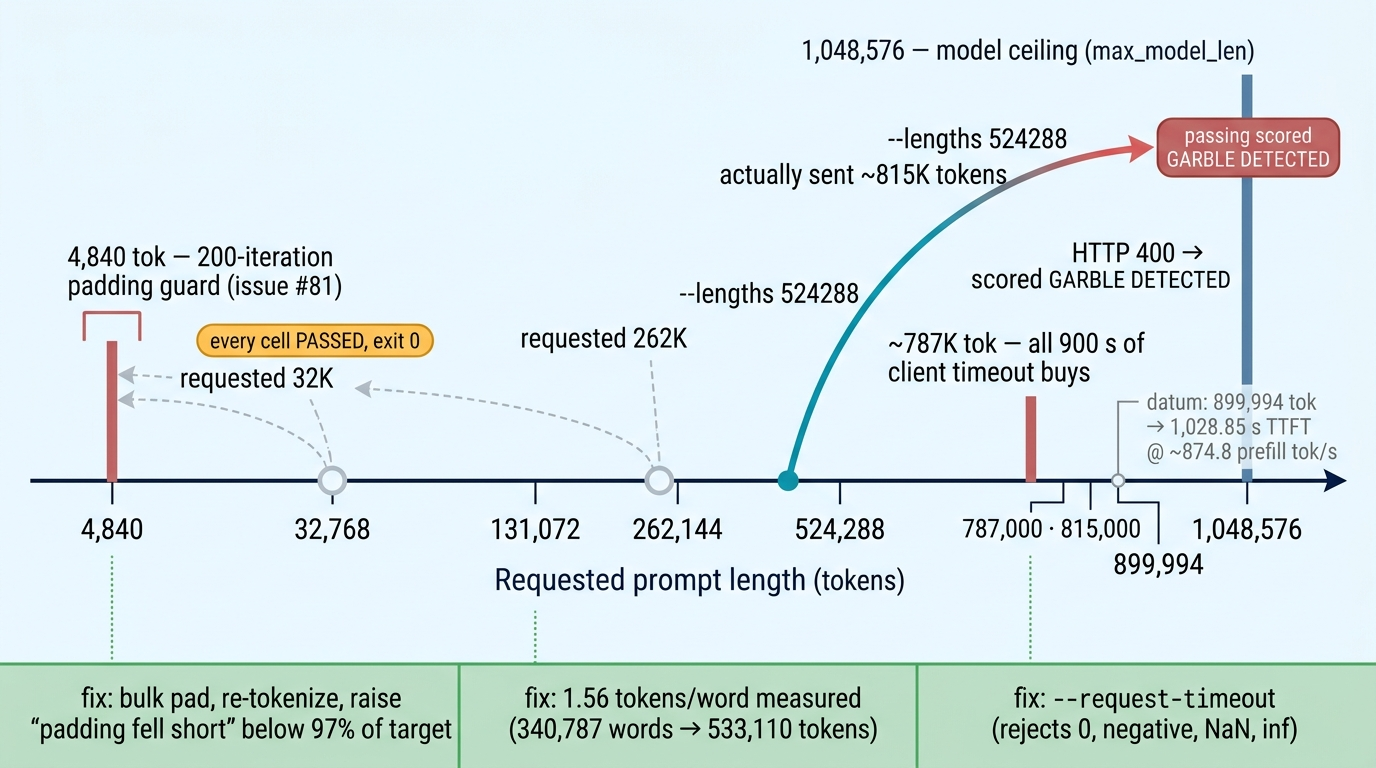
\includegraphics[width=\textwidth]{figures/ch10-instrument-ceilings.png}
\caption{Three ceilings that were not the model's. On one length axis: the
200-iteration padding guard flattened every deep RULER cell to
\textasciitilde{}4{,}840 tokens while exiting 0 (\ghissue{81}); the
1.3-words-per-token heuristic turned a 524{,}288-token request into
\textasciitilde{}815K and past the 1{,}048{,}576 ceiling, so a correct
HTTP~400 was scored \texttt{GARBLE DETECTED}; and the harness's own
900\,s timeout buys only \textasciitilde{}787K tokens of prefill against
the recorded 899{,}994-token / 1{,}028.85\,s datum. Only the steel rule at
1{,}048{,}576 belongs to the model.}
\label{fig:measure-ceilings}
\end{figure}

\begin{hblesson}
The instrument is a suspect too. The padding bug made deep cells test
shallow context while reporting success; the client timeout converted its
own limit into a model verdict; SSE counting undercounted 4.5$\times$; a
label-order assumption silently emptied the acceptance curve. Each bug got
what serving bugs get: a root cause, a fix, and a permanent regression
suite (\repofile{test-ruler-lite-pad.py}, \repofile{test-spec-acceptance.py},
\repofile{test-responses-api-live.py}, \repofile{test-boot-shape-warmup.sh})
--- several of which keep the original bug as a checked-in negative
control. If a benchmark gates releases, it deserves tests exactly as much
as the code it gates.
\end{hblesson}

\section{Live verifiers as release gates}

The six-phase audit is the broad, periodic gate; a fix that changes one
contract needs something sharper. Beyond the periodic audit, therefore,
specific fixes ship with dedicated live
verifiers --- scripts that hit a running endpoint and prove a contract
holds, run as gates before a change is declared done
(\Cref{ch:patches,ch:bugs}). The section's governing principle comes from
\repofile{docs/PATCHES.md}: \emph{``The JSON request report alone is not
the complete live gate.''} A verifier can only see what the API surface
shows it; the failure modes that matter most (a wedged pair, a silent
stream truncation) show up in logs and health state first. Every gate below
is therefore a conjunction --- a case report \emph{plus} log and counter
evidence --- and each of its assertions exists because of a specific
failure it would catch. What distinguishes the verifiers below is not the
endpoints they hit but the disciplines they demonstrate: gates that reach
past request shape into engine behavior, a bounded case matrix whose verdict
includes both ranks' logs, and mode strictness, where a verifier asserts the
behavior the deployment was configured for rather than accepting either
outcome.

\subsection{The Responses API verifier}

\repofile{scripts/verify-responses-api-live.py} is the deep contract check
for the \code{/v1/responses} surface. It runs exact-text and strict
JSON-schema gates; the strictest SSE frame validator in the repository (exactly
one \code{response.completed}, last, with integer usage; concatenated
deltas must reproduce the non-streaming text); and three gates that go past
request/response shape into engine behavior:

\begin{itemize}
\item \textbf{Store LRU} exists to catch a FIFO store masquerading as LRU
  --- an eviction policy that would silently drop a conversation's most
  recently used context. The mechanism: fill the response store to its
  declared capacity, \emph{touch} the oldest entry via GET, roll over with
  one more POST, and require that the touched entry survives while the
  true least-recently-used entry returns 404.
\item \textbf{Appended multi-turn cache floor} exists to catch a prefix
  cache that quietly stops hitting on append-only conversations --- the
  exact workload agents generate. The mechanism: a tokenize-verified
  \textasciitilde{}21K nonce'd prefix, six appended turns with exact
  sentinels, and from turn 2 on an \emph{engine-aware} floor on
  \code{usage.prompt_tokens_details.cached_tokens},
  $\lfloor(\text{prompt}-4096)/256\rfloor \times 256$, derived from the
  sliding-window and block sizes --- a minimum cache-hit guarantee, not a
  vague ``caching works.''
\item \textbf{Disconnect} exists to catch orphaned decode --- an engine
  that keeps generating for a client that hung up, burning slots invisible
  to any per-request view. The mechanism: open a raw stream with
  \code{ignore_eos}, confirm via \code{/metrics} that the request is
  running, close the socket, and validate an entire counter chain.
  Running and waiting must drain to zero within a bounded window; counters
  stay monotonic; the successful-request counter at idle equals its
  pre-request value (an abort must \emph{not} count as a success); only a
  bounded handful of tokens post-open; and generation frozen after idle.
\end{itemize}

\subsection{The issue-136 canary: logs are part of the gate}

The \ghissue{136} XGrammar-termination backport (a grammar-state desync
under speculative decoding, \Cref{ch:bugs}) ships with a bounded live
canary, \repofile{scripts/verify-issue136-xgrammar-live.py}: 20 sequential
strict-tool cases, 100 concurrent cases at concurrency 4 alternating
required and named \code{tool_choice}, five \code{ignore_eos} strict-schema
cases that deliberately force generation \emph{past} grammar termination
(the exact upstream failure trigger), ten ordinary-tool controls, and ten
plain-chat controls. That is 145 cases, health-checked before and after,
with a deliberately redacted JSON report that never contains request
bodies, response bodies, or credentials.

\begin{lstlisting}[language=bash]
VLLM_API_KEY='...' python3 scripts/verify-issue136-xgrammar-live.py \
  --base-url http://127.0.0.1:8888/v1 \
  --model deepseek-v4-flash-dspark \
  --output /tmp/issue136-xgrammar-live.json
\end{lstlisting}

But the documented gate is explicitly larger than the verifier's report.
Per \repofile{docs/PATCHES.md}, from the saved UTC start time both rank
logs must contain \emph{zero} matcher-termination warnings, zero
\code{Failed to advance FSM} / grammar-rejection lines, zero shared-memory
broadcast-block waits, zero \code{sample_tokens} timeouts, and zero
engine-dead errors; container restart counts must remain unchanged; and no
request may remain running with frozen generation progress. This is the
section's opening principle made concrete: the gate is the conjunction of
the 145/145 report, the both-rank log sweep, and the health/restart
evidence --- never the JSON report alone.

\subsection{Mode-strict verification: issue 138}

\repofile{scripts/verify-issue138-responses-history-live.py} guards the
Responses-API full-history replay fix (\ghissue{138}) and demonstrates a
third verifier discipline: \textbf{mode strictness}. The flag
\code{--expect-legacy rejected|accepted} is mandatory, and the verifier
asserts the \emph{configured} behavior --- ``not either outcome passes.''
In rejected mode, a legacy type-less assistant item must yield HTTP~400
with a numeric error code and a message naming the offending field; in
accepted mode it must yield exactly 200. The verifier then proves three
more things: semantic continuity (a fact stated in a legacy item must be
recallable, showing the item participates in context rather than merely
parsing); that six malformed negative variants still 400 (the
compatibility patch must not become a validation hole); and that three
canonical positive controls still 200. A verifier that passes on ``either
behavior'' would silently bless a mis-deployed flag; mode strictness makes
the deployment configuration itself part of the assertion. Both this
verifier and the Responses verifier have their own CPU test suites that
replay fake endpoints against them and pin the exact shape of every request
they make --- the instruments are under test, all the way down.

\section{CPU CI versus live gates}

Every gate so far has needed a live endpoint --- but most of what the repository
proves, it proves without one. The repository runs two disjoint evidence systems,
and knowing which claims each
can make is itself measurement discipline. \repofile{scripts/ci-validate.sh}
is the CPU-only gate chain (also the GitHub Actions workflow): shell syntax
and Python compilation over every script, \textasciitilde{}33 hermetic unit
suites, and a long section of regression-guard greps that freeze past
incidents as executable memory. What CPU CI \emph{can} enforce:

\begin{itemize}
\item \textbf{Wiring, defaults, and fail-closed behavior}: every hotfix
  must be default-off, gated on an exact-\code{1} env comparison, invoked
  fail-closed (\code{|| exit 1}), and synced to the worker --- four
  properties, each independently grepped per patch, and behaviorally
  re-proven by stub-driven suites (\Cref{ch:patches}). Injected-fault
  tests complete the proof: they make \code{os.replace} fail on the
  $N$-th call, corrupt bytes after publish, and interrupt verification
  reads, proving every patcher rolls back to exact original bytes and
  permissions.
\item \textbf{Fixture SHA triangulation}: patches are byte-transformations
  between pinned states. Fixture hashes, patcher constants, and
  test-local literal hunks are three independent legs that must agree ---
  replaying the test's own copy of a hunk over the pinned stock fixture
  must reproduce the pinned post fixture byte-for-byte. One backport is
  even verified against the official upstream merge by Git blob SHA-1.
\item \textbf{Emulated semantics}: \repofile{scripts/verify-dsv4-027-equality-gate.py}
  proves a GPU patch safe without a GPU by pinning the constants, emulating
  the gate arithmetic on CPU, and sweeping the integer-division boundary.
\end{itemize}

What only the live pair can establish: actual \tokspersec{}, kernel behavior
(JIT storms, autotune tactics, CUDA-graph capture coverage), and
tensor-parallel behavior (collective timing, watchdog interactions,
\ghissue{117}-class hangs). CPU CI can prove the recipe \emph{says} what it
should and fails \emph{how} it should; only the audit and the verifiers can
prove the deployment \emph{performs}. The repository never lets one system claim
the other's territory --- \repofile{ci-validate.sh}'s own header says it
``does NOT run the live 2$\times$ Spark serve, decode bench, or
tool-eval-bench.''

\subsection{Double-entry measurement bookkeeping}

Bridging the two systems is the most transferable idea in this chapter:
every live claim is booked twice, once client-side and once server-side,
and the entries must agree. The prefix-cache repro (\ghissue{26}) counts a hit only when
per-lane \code{usage.prompt_tokens_details.cached_tokens} \emph{and} the
server's \code{prefix_cache_hits_total} delta are both positive. The
starvation repro derives its decode rate from a forced exact output-token
count and then verifies it against the \code{generation_tokens_total}
delta. The disconnect gate's entire verdict is a counter chain. A
client-side impression that the server's own counters do not corroborate is
treated as an instrument bug until proven otherwise --- which is exactly
how the SSE undercount was caught (\Cref{fig:measure-double-entry} sets the
three pairings side by side as a ledger).

\begin{figure}[htbp]
\centering
\adjustbox{max width=\textwidth}{%
\begin{tikzpicture}[font=\small]
  % --- column headers -------------------------------------------------------
  \node[hbnode,text width=54mm,align=center,fill=navy,draw=navy,
        text=white,font=\small\bfseries] (ch) at (3.2,0) {CLIENT-SIDE ENTRY};
  \node[hbnode,text width=54mm,align=center,fill=brandgray,draw=brandgray,
        text=white,font=\small\bfseries] (sh) at (11.0,0) {SERVER-SIDE ENTRY};
  % --- row 1: prefix-cache repro (both entries must be positive) ------------
  \node[hbbox,text width=54mm,align=center,font=\scriptsize] (c1) at (3.2,-1.9)
    {\ttfamily usage.prompt\_tokens\_details.\\cached\_tokens};
  \node[hbgpu,text width=54mm,align=center,font=\scriptsize] (s1) at (11.0,-1.9)
    {\ttfamily prefix\_cache\_hits\_total ($\Delta$)};
  \node[hbnode,fill=ice,draw=teal,font=\scriptsize,inner sep=3pt,
        minimum height=6mm] (and1) at (7.1,-1.9) {AND};
  \draw[hbarrow,<->,color=teal] (c1.east) -- (and1.west);
  \draw[hbarrow,<->,color=teal] (and1.east) -- (s1.west);
  \node[hbpatch,font=\scriptsize,inner sep=3pt,minimum height=6mm,anchor=west]
    (i26) at (14.4,-1.9) {issue \ghissue{26}};
  \draw[hbarrow,color=amber!80!black] (i26.west) -- (s1.east);
  \node[hblabel,anchor=south] at (7.1,-1.18) {entries must agree};
  % --- row 2: starvation repro ---------------------------------------------
  \node[hbbox,text width=54mm,align=center,font=\scriptsize] (c2) at (3.2,-3.6)
    {forced exact output-token count};
  \node[hbgpu,text width=54mm,align=center,font=\scriptsize] (s2) at (11.0,-3.6)
    {\ttfamily generation\_tokens\_total ($\Delta$)};
  \draw[hbarrow,<->,color=teal] (c2.east) -- (s2.west);
  % --- row 3: disconnect gate = a counter chain -----------------------------
  \node[hbbox,text width=54mm,align=center,font=\scriptsize] (c3) at (3.2,-6.9)
    {socket closed after \texttt{/metrics} confirms request running};
  \node[hbgpu,text width=54mm,align=center,font=\scriptsize] (k1) at (11.0,-5.2)
    {running / waiting $\to$ 0 (bounded window)};
  \node[hbgpu,text width=54mm,align=center,font=\scriptsize] (k2) at (11.0,-6.4)
    {counters monotonic};
  \node[hbgpu,text width=54mm,align=center,font=\scriptsize] (k3) at (11.0,-7.6)
    {successful-request counter unchanged (abort $\neq$ success)};
  \node[hbgpu,text width=54mm,align=center,font=\scriptsize] (k4) at (11.0,-8.9)
    {bounded tokens post-open; generation frozen at idle};
  \draw[hbarrow,color=brandcyan] (k1) -- (k2);
  \draw[hbarrow,color=brandcyan] (k2) -- (k3);
  \draw[hbarrow,color=brandcyan] (k3) -- (k4);
  \draw[hbarrow,<->,color=teal] (c3.east) -- (8.1,-6.9);
  % --- verdict rail ---------------------------------------------------------
  \node[hbpatch,text width=58mm,align=left,font=\small] (rule) at (3.4,-10.7)
    {\textbf{disagreement $\Rightarrow$ instrument bug until proven
     otherwise}};
  \node[hbwarn,text width=70mm,align=left,font=\scriptsize] (sse) at (11.2,-10.7)
    {caught here: SSE chunk counting undercounts $\approx$4.5$\times$
     $\to$ count \texttt{usage.completion\_tokens}\\[2pt]
     {\ttfamily stream\_options=\{"include\_usage": true\}}};
  \draw[hbfail] (sse.north) -- (7.1,-9.7);
  \begin{scope}[on background layer]
    \node[hbgroup,fit=(ch)(c1)(c2)(c3)] {};
    \node[hbgroup,fit=(sh)(s1)(s2)(k1)(k4)] {};
  \end{scope}
\end{tikzpicture}%
}
\caption{Double-entry measurement bookkeeping. Every live claim is booked
once client-side and once server-side, and a claim is a result only when
both entries agree: the prefix-cache repro requires \code{cached_tokens}
\textbf{and} a positive \code{prefix_cache_hits_total} delta (\ghissue{26});
the starvation repro checks its forced output-token arithmetic against
\code{generation_tokens_total}; the disconnect gate is nothing but a counter
chain. A client-side impression the server's counters do not corroborate is
an instrument bug until proven otherwise --- which is exactly how the
$\approx$4.5$\times$ SSE undercount was caught.}
\label{fig:measure-double-entry}
\end{figure}

\section{Benchmark noise and statistics}

Even a number booked correctly on both sides of the ledger can mislead if
the trial count cannot support the claim hung on it. The final discipline is
statistical honesty about what a number of trials
can resolve. Single-stream decode on this lane swings with the prompt
drawn: identical c=1 trials range roughly 48--76~\tokspersec{}, and the working
noise figure is $\pm$10~\tokspersec{} at c=1. Three trials cannot resolve a
1--3\% knob --- a fact the 2026-09-02 A/B session learned when a
single-PF-vs-dual-PF fabric diagnostic produced 65.7 then 54.8~\tokspersec{}
across repeats: statistically a tie, not a fabric problem. The protocol
that emerged (\repofile{scripts/ab-boot.sh}, \Cref{ch:perf}): pool
\textbf{8 trials} per condition per boot (three from the measurement dossier
plus five extra, precisely because ``c=1 noise on this lane is
\textasciitilde{}$\pm$10 tok/s''), report medians, compare whole
distributions against a \emph{same-day} baseline, and demand separation.
A knob is ON only when its trials clear the baseline's range, not its
mean --- the three verdict shapes that rule produces are drawn in
\Cref{fig:measure-separation}.

\begin{figure}[htbp]
\centering
\adjustbox{max width=\textwidth}{%
\begin{tikzpicture}[font=\small]
  % ---- the deciding edge: the LOWER edge of the baseline range -------------
  \draw[dashed,thick,color=navy] (6.0,2.60) -- (6.0,7.0);
  \node[hbtitle,anchor=south,font=\scriptsize\bfseries] at (6.0,7.05)
    {baseline minimum --- the edge that decides};
  % ---- lane 1: separated BELOW the baseline range -> OFF ------------------
  \draw[fill=lightgray,draw=brandgray] (6.0,6.12) rectangle (9.0,6.68);
  \node[hblabel,font=\tiny,anchor=base] at (8.2,6.34) {baseline};
  \draw[thick,color=navy] (7.4,6.12) -- (7.4,6.68);
  \draw[fill=clueerror!20,draw=clueerror!70!black] (2.4,6.12) rectangle (5.2,6.68);
  \draw[thick,color=navy] (4.0,6.12) -- (4.0,6.68);
  \node[hbwarn,font=\scriptsize,inner sep=3pt,minimum height=5mm,anchor=west]
    at (12.7,6.4) {OFF};
  % ---- lane 2: separated ABOVE the baseline range -> ON -------------------
  \draw[fill=lightgray,draw=brandgray] (6.0,4.82) rectangle (9.0,5.38);
  \node[hblabel,font=\tiny,anchor=base] at (8.2,5.04) {baseline};
  \draw[thick,color=navy] (7.4,4.82) -- (7.4,5.38);
  \draw[fill=brandgreen!18,draw=brandgreen!70!black] (9.9,4.82) rectangle (12.3,5.38);
  \draw[thick,color=navy] (11.2,4.82) -- (11.2,5.38);
  \node[hbgpu,font=\scriptsize,inner sep=3pt,minimum height=5mm,anchor=west]
    at (12.7,5.1) {ON};
  % ---- lane 3: overlapping the baseline range -> tie ----------------------
  \draw[fill=lightgray,draw=brandgray] (6.0,3.52) rectangle (9.0,4.08);
  \node[hblabel,font=\tiny,anchor=base] at (6.7,3.74) {baseline};
  \draw[thick,color=navy] (7.4,3.52) -- (7.4,4.08);
  \draw[fill=amber!45,draw=amber!80!black,fill opacity=0.55]
    (7.6,3.52) rectangle (10.6,4.08);
  \draw[thick,color=navy] (9.1,3.52) -- (9.1,4.08);
  \node[hbpatch,font=\scriptsize,inner sep=3pt,minimum height=5mm,anchor=west]
    at (12.7,3.8) {OFF (tie)};
  % ---- raw spread of this lane, and the working noise figure --------------
  \draw[fill=lightgray!40,draw=brandgray!50] (2.2,2.60) rectangle (12.9,3.10);
  \node[hblabel] at (7.55,2.85) {c=1 trials on this lane: 48--76 \tokspersec{}};
  \draw[hbarrow,<->,color=teal] (2.2,2.25) -- (3.4,2.25);
  \node[hblabel,anchor=west] at (3.55,2.25)
    {working noise figure: $\pm$10 \tokspersec{} at c=1};
  % ---- schematic axis (no ticks: per-trial values are not published) ------
  \draw[hbarrow] (1.8,1.55) -- (13.9,1.55);
  \node[hblabel,anchor=north east] at (13.9,1.42)
    {decode \tokspersec{} --- schematic axis; per-trial values are not published};
  % ---- the three verdicts, keyed to the lanes -----------------------------
  \draw[fill=clueerror!20,draw=clueerror!70!black] (1.8,0.75) rectangle (2.1,0.95);
  \node[hblabel,anchor=west] at (2.25,0.85)
    {TC-decode: c=1 46 vs 55; 7 of 8 trials below baseline minimum $\to$ OFF};
  \draw[fill=brandgreen!18,draw=brandgreen!70!black] (1.8,0.35) rectangle (2.1,0.55);
  \node[hblabel,anchor=west] at (2.25,0.45)
    {capture size 48: c=6 aggregate 139 vs 122 $\to$ ON (reversal A/B: un-fix
     and watch it fall)};
  \draw[fill=amber!45,draw=amber!80!black] (1.8,-0.05) rectangle (2.1,0.15);
  \node[hblabel,anchor=west] at (2.25,0.05)
    {indexer logits 512: $-1.5$/$-1.8$\% inside $\pm$2\% noise $\to$ OFF
     (tie), retry on a $\geq$256K sweep};
  % ---- conditions, and the counter-example ---------------------------------
  \node[hblabel,anchor=north west,align=left] at (1.8,-0.45)
    {8 pooled trials per condition per boot\\same-day baseline\\medians reported};
  \node[hbfaint,font=\scriptsize,text width=62mm,align=left,anchor=north east]
    at (13.9,-0.4)
    {single-PF vs dual-PF: 65.7 then 54.8 across repeats --- a tie, not a
     fabric problem};
\end{tikzpicture}%
}
\caption{A knob is ON only when its trials clear the baseline's
\emph{range}, not its mean. With c=1 trials on this lane ranging
48--76~\tokspersec{} and a working noise figure of $\pm$10~\tokspersec{},
three trials cannot resolve a 1--3\% knob: the 2026-09-02
single-PF-vs-dual-PF diagnostic produced 65.7 then 54.8~\tokspersec{} and
was a tie. Pooling eight trials per condition per boot against a same-day
baseline yields the three verdict shapes applied in \Cref{tab:ab-verdicts}
--- separated below (TC-decode, OFF), separated above (capture size 48, ON,
decided by a reversal A/B), and overlapping (indexer logits 512, tie). The
axis is schematic: per-trial values are not published and are not drawn.}
\label{fig:measure-separation}
\end{figure}

\begin{table}[htbp]
\centering\small
\caption{How 8-trial pooling decided knobs in the September 2026 A/B
sequences. ``Separation'' verdicts cite distribution overlap, not point
estimates.}
\label{tab:ab-verdicts}
\begin{tabular}{@{}ll>{\raggedright\arraybackslash}p{7.0cm}@{}}
\toprule
Knob & Verdict & Evidence (pooled trials, medians) \\
\midrule
TC-decode & OFF & c=1 46 vs.\ 55; 7 of 8 trials below baseline \emph{minimum} \\
Markov replication & OFF & acceptance unchanged; c=6 aggregate 122 vs.\ 148 \\
Capture size 48 & ON & c=6 aggregate 139 vs.\ 122 at 42; all capture-42 trials below base min \\
Inflight prefills = 2 & ON (later demoted) & c=4 8K TTFT spread 9.1 vs.\ 14.6\,s; all trials below base's best --- verdict withdrawn once the \code{r3} admission-count repair landed \\
Indexer logits 512 & OFF (tie) & $-1.5$/$-1.8$\% inside $\pm$2\% noise; retry on a $\geq$256K sweep \\
\bottomrule
\end{tabular}
\end{table}

Two entries in \Cref{tab:ab-verdicts} deserve emphasis as method. The
capture-size verdict came from a \emph{reversal} A/B, a design pattern in
its own right: when the fix is already live, un-fix it briefly. The
suspected fix was reverted and the metric watched to fall
(139\,$\to$\,122) --- the cleanest causal design available on a
production box, because the falling edge rules out every confound the
rising edge cannot. And the inflight-prefills verdict \emph{overturned} an
earlier same-repository decision (\ghissue{154} had reverted the knob to 1 on
fairness grounds); the later measurement, with pooled trials, put it back.
That verdict has since been demoted in turn. The \code{r3} admission-count
repair (PR~\ghissue{211}) made the \ghissue{27} gate count in-flight partial
prefills exactly from \code{self.running}, and the shipped default returned
to 1: the A/B above ran on the pre-\code{r3} undercounting scheduler and, in
the repository's own words, ``does not establish post-r3 behavior.'' Cap 2 keeps
unit coverage but no post-\code{r3} live qualification. Which is the lesson
twice over --- measure the code you run today rather than trusting old
A/Bs, including the A/B you ran last month.

\begin{hbwarstory}
The cost of skipping this discipline is a retraction. The \ghissue{143}
stability matrix claimed an admission-cap mechanism:
``\code{MAX_NUM_SEQS=16} bad / 32 safe.'' The repository's own
\repofile{.env.dspark.example} now carries the verdict in capitals --- the
mechanism is \textbf{RETRACTED}, because ``every cell in that matrix was
n=1; per-burst failure probability explains the whole table without an
admission-cap effect.'' The underlying \ghissue{141} stalls are stochastic
per burst: one configuration ran three clean bursts and died on the
fourth; another died on a fresh-boot first burst. With per-burst failure
probabilities, an $n{=}1$ grid is a random bitmap that will always contain
a plausible-looking pattern. The file's conclusion is the doctrine: ``a
single clean burst cannot distinguish a safe configuration from a lucky
one'' --- and no tested value is declared generally safe.
\end{hbwarstory}

\begin{figure}[htbp]
\centering
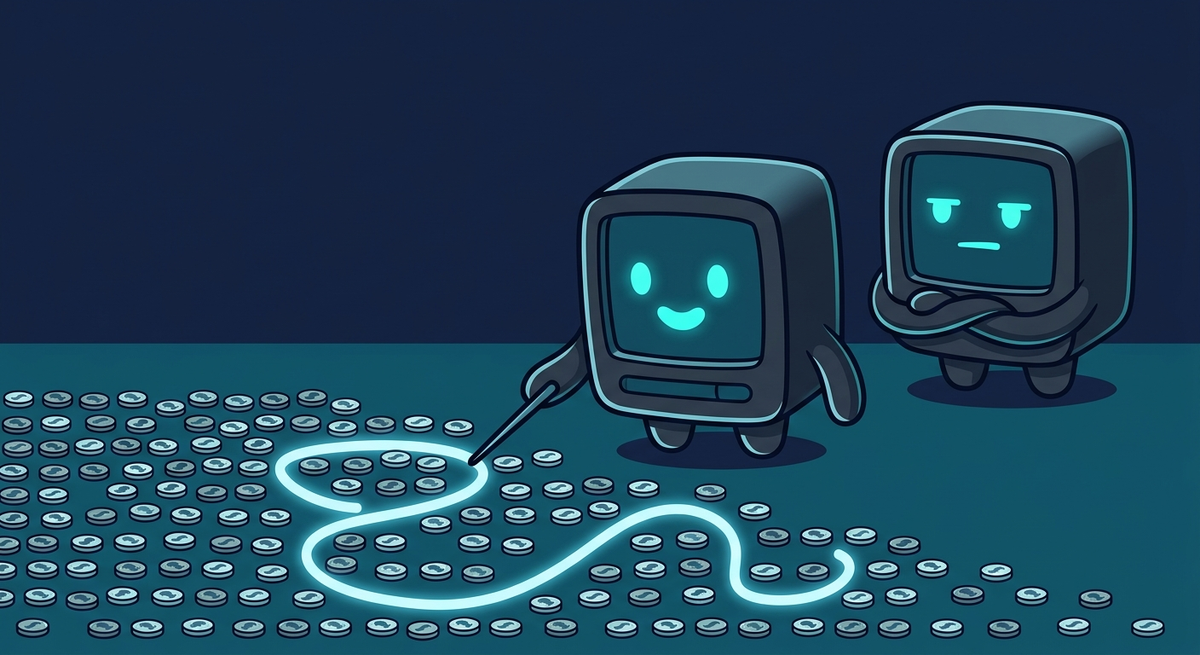
\includegraphics[width=0.80\textwidth]{figures/toon-ch10-pareidolia.png}
\caption{Every cell was $n{=}1$. With a per-burst failure probability, a grid of single trials is a random bitmap, and a random bitmap will always contain a plausible-looking pattern for a willing reader to trace. The \ghissue{143} stability matrix published one such pattern as an admission-cap mechanism and later retracted it in capitals. A single clean burst cannot distinguish a safe configuration from a lucky one.}
\label{fig:toon-pareidolia}
\end{figure}

The same honesty governs publication. The dated results ledger
(\repofile{results/RESULTS-2026-08-14.md}) opens with a glossary
disambiguating every marketing-adjacent number: ``1M context'' is a
per-request ceiling, not six chats each holding a million tokens; aggregate
\tokspersec{} is fleet-wide generation, not what one user feels. Each
matrix names its exact method (unique cold prefixes, thinking off,
pinned output length) and its raw JSON companion. Every measurement dossier
from \repofile{scripts/ab-measure.sh} prints its expected reference range
inline with each section, so a results file is self-judging months later.
Numbers without a replayable method are, in this repository's culture, not
results; they are anecdotes awaiting retraction.

The benchmark has changed category. It is not a neutral observer reporting
on the serving stack; it is a second program running against production,
with its own bugs, its own regression suite, and its own demonstrated
capacity to manufacture a 40\% regression out of a prompt or a
4.5$\times$ slowdown out of a chunk count. What a number means has
narrowed accordingly: not what the client felt, but a decode-only window,
booked twice against the server's own counters, pooled across enough
trials to clear a same-day baseline's range, and replayable from a
recorded method. The figure printed in a results file is the last line of
a document that also has a methodology, a noise band, and an expiry date
--- and any of those three can retract it.

\FloatBarrier
\section*{Takeaways}

\begin{itemize}
\item Measurement bugs masquerade as model regressions, and the
  misattribution runs the expensive way: a model regression costs a
  rollback and a re-quantize, an instrument bug costs a script fix. Both
  founding false alarms --- the fake \textasciitilde{}45~\tokspersec{}
  drafter collapse and the correct HTTP~400 scored
  \texttt{GARBLE DETECTED} --- came from the instrument, not the model.
\item Five principles, all mechanized rather than remembered:
  tokenize-verified lengths (never the 1.3-words-per-token heuristic),
  cold nonce'd prefills, natural task prompts, decode-only windows that
  exclude TTFT and warmup, and \code{usage.completion_tokens} instead of
  SSE chunk counts, which undercount by $\approx$4.5$\times$ when MTP
  packs accepted tokens into one delta.
\item The instrument is under test too: every benchmark bug got a root
  cause, a fix, and a permanent regression suite --- several keeping the
  original bug alive as a checked-in negative control, like the
  200-iteration pad loop that ceilinged deep RULER cells at 4{,}840
  tokens while exiting 0 (\ghissue{81}).
\item A JSON pass report alone is not a release gate. A live gate is a
  conjunction --- case report, both ranks' logs, counter deltas, and
  health/restart evidence --- and every live claim is booked double-entry,
  client-side and server-side, with disagreement treated as an instrument
  bug until proven otherwise.
\item Respect the noise: at $\pm$10~\tokspersec{} on this lane, three
  trials cannot resolve a 1--3\% knob, so pool eight per condition per
  boot, compare medians against a same-day baseline, and demand
  distribution separation --- and when an n=1 matrix slips through
  (\ghissue{143}), retract it in public.
\end{itemize}

\chaptertransition{A gate is only worth building if there is a healthy pair
to point it at, and this cluster lost far more serving time to ordinary
operational acts done in the wrong order than to anything a benchmark could
catch. The next chapter is the runbook the audit quietly assumes: the
worker-first boot, the exit-code contract, weights logistics, JIT-cache
doctrine, and the incident-response sequence for the day the pair freezes.
It opens on the most disorienting state this topology can reach --- two
containers that each look individually healthy while the tensor-parallel
group between them is dead or stale, and a launcher whose exit code cannot
tell you which.}

% =============================================================================
% Chapter 11 — Operations: Running the Pair
% =============================================================================
\chapter{Operations: Running the Pair}
\label{ch:operations}

\code{docker compose up} is one line. The launcher that actually starts this
cluster, \repofile{start-deepseek-v4-flash-dspark.sh}, is a 1{,}753-line
shell program. The gap between those two numbers is the subject of this
chapter. A two-node tensor-parallel serving pair is one distributed system
pretending to be one server: every operational act --- starting, stopping,
checking, updating weights --- must happen on \emph{both} ranks, in the
right order, with the same configuration bytes. Otherwise the pair degrades
into the worst failure mode in distributed serving: two containers that each
look individually fine while the TP group between them is dead or stale.

This chapter is the runbook for the repository's operational surface --- the
launcher, the stop/status/smoke/prepare scripts, the JIT-cache and warmup
doctrine, and the incident-response machinery --- with the rationale behind
each rule. On this stack, almost every rule is a scar from a numbered
incident. The worker-first boot order, the exit-code contract, the
persisted-cache doctrine, the flight-recorder wiring: each exists because
its absence once took the pair down.

For an inference engineer, this is the chapter where availability is
actually decided. The incidents that cost this cluster the most serving time
were not exotic kernel faults; they were ordinary operational acts done in
the wrong order --- a restart issued while a rank was still loading, a
stale worker left serving after a head-only reboot, a JIT cache discarded
on container recreate that later killed the pair through the 600\,s NCCL
watchdog. Serving performance is earned in the other chapters; whether
anyone gets to experience it is earned here.

\section{The lifecycle of a start}
\label{sec:ops-lifecycle}

The launcher's 1{,}753 lines are organized as a strict pipeline: normalize
configuration, validate everything that can be
validated cheaply, synchronize files to the worker, preflight every risky
patcher, and only then start containers --- worker first, head second.
After that it polls health, fires a smoke request, and hands off to the
warmup sweep.
\Cref{fig:ops-boot-swimlane} shows the whole sequence. The ordering follows
one invariant: every check that can fail is placed where failing is free ---
before either node has a container, and, where a check genuinely needs a
container, inside a throwaway one.

\subsection{One private environment snapshot}

\repofile{.env.dspark} may carry API keys, and it does not stay on the head:
the launcher ships a copy to the worker node so both ranks consume identical
configuration bytes. Everything the launcher does with the file follows from
those stakes. It never sources the operator's file directly: it copies it
through \code{sed} to strip a UTF-8 BOM and CR line endings, into a
\code{mktemp} file chmod'ed to \code{0600}, and sources \emph{that}. The
same snapshot is then reused as the \code{--env-file} for every Compose
invocation (\code{COMPOSE_DISABLE_ENV_FILE=1} ensures Compose sees only this
file). The operator's file stays byte-identical; head, Compose, and worker
all consume one normalized copy (PR \ghissue{98}).

The worker's copy is published the same way: streamed over ssh into a
private \code{umask 077} sibling file and renamed atomically with
\code{mv -f}, so a failed transfer can neither truncate nor expose the
previous environment file.

The snapshot is also where the launcher enforces its ambient-credential guard:
\envvar{DSPARK_API_KEYS} set in the calling shell but differing from the env
file is an immediate exit 2, because a probe must never authenticate with a
different key set than the server was started with.

\subsection{Validation before side effects}

Between snapshot and sync, the launcher runs a battery of checks that all fail
\emph{before} anything is created on either node:

\begin{itemize}
  \item \textbf{Numeric knobs.} \repofile{dspark-numeric-knobs.sh} validates
    \envvar{MAX_NUM_SEQS}, \envvar{MTP_NUM_TOKENS}, and
    \envvar{MAX_NUM_BATCHED_TOKENS} (\Cref{sec:ops-hygiene}) and rewrites the
    snapshot so both ranks see identical normalized decimals.
  \item \textbf{Speculative constraints.} On Vision-Exp,
    \envvar{MTP_NUM_TOKENS} must be $\geq 5$ and divisible by 3
    (\code{num_nextn_predict_layers=3}), unless the block-$k$ unlock is enabled;
    \envvar{DRAFT_SAMPLE_METHOD} must be exactly \code{probabilistic} or
    \code{greedy}. Anything else exits 2 here rather than at boot.
  \item \textbf{Fabric identity.} With \envvar{NCCL_IB_GID_AUTO}=1 (the
    default), the launcher runs a sysfs resolver on \emph{each} node that
    mirrors NCCL's own \envvar{NCCL_IB_HCA} selector semantics (prefix
    vs.\ exact match, port fields parsed the way \code{atoi} would, the
    32-device cap) and verifies every selected HCA/port exposes a usable
    RoCEv2/IPv4 GID --- failing closed if any member has none. It deliberately
    pins nothing: after issue \ghissue{38}-family field reports, a pinned
    global GID index was found to wedge NCCL init on dual-HCA nodes after
    link events. Auto mode therefore validates and then leaves
    \envvar{NCCL_IB_GID_INDEX} unset so NCCL picks per HCA
    (see \Cref{ch:fabric}).
  \item \textbf{Presence preflights.} Passwordless ssh to the worker, the
    pinned image present on \emph{both} nodes, the port free on the head, and
    no existing containers for the project on either node.
\end{itemize}

\subsection{Sync, render, preflight, then start --- worker first}

File sync pushes the compose file, the atomically-published env snapshot, the
DSpark proposer bind-mount source, and roughly twenty hotfix patchers into the
worker checkout, one \code{scp} per patch, so the worker's entrypoint applies
byte-identical patches. Then \code{docker compose config --quiet} renders the
config on the head and (over ssh) on the worker --- validation by rendering,
catching interpolation errors before any container exists. Every fail-closed
patcher that supports it (\code{--check} preflights for the Responses store,
issue \ghissue{117}'s SHM ring recheck, \ghissue{136}, \ghissue{191}, the
block-$k$ unlock) is then dry-run \emph{worker first, then head}, inside
throwaway \code{compose run --rm --no-deps} containers. An incompatibility on
either rank aborts the start while zero services are running.

Only now do the services come up, and the order is a rule with a war story
behind it: \textbf{worker (rank 1, \code{HEADLESS=1}) first, head (rank 0)
last}. The head owns the distributed rendezvous --- the TCPStore at
\envvar{MASTER_ADDR}:\envvar{MASTER_PORT} --- and rank 1 blocks on it while
loading. Bringing the head up last means the rendezvous is created once,
consumed once, and never torn down under a peer that is mid-load.

\begin{hbwarstory}
Issue \ghissue{38}: ``Worker Exited (1) on every start.'' The original launcher
applied its \code{.sh} hotfixes \emph{after} \code{compose up}, then issued a
\code{compose restart}/\code{stop} while vLLM was still loading --- tearing down
the head's TCPStore underneath rank 1 (or hanging the operator on
``Stopping''). The fix restructured the whole boot: hotfixes moved into the
compose entrypoint, running \emph{before} \code{exec vllm}, so a start never
has to bounce a freshly booting pair. The worker-first ordering and the
``no mid-boot stop'' rule both date from this incident.
\end{hbwarstory}

\begin{figure}[htbp]
\centering

\includegraphics[width=0.80\textwidth]{figures/toon-ch11-rugpull.png}
\caption{Meant helpfully, timed catastrophically. The original launcher applied its hotfixes \emph{after} \code{compose up}, then issued a restart while vLLM was still loading --- tearing the head's TCPStore out from under rank~1 and producing ``Worker Exited (1)'' on every single start. Moving the hotfixes into the compose entrypoint, before \code{exec vllm}, means a start never has to bounce a pair that is still coming up.}
\label{fig:toon-rugpull}
\end{figure}

\subsection{Health wait, smoke, warmup handoff}

After \code{up -d} on both ranks the launcher polls the authenticated
\code{/v1/models} endpoint --- up to \envvar{WAIT_ATTEMPTS}=100 tries,
\envvar{WAIT_SECONDS}=15 apart (about 25 minutes; a first boot with cold JIT
caches genuinely needs it). Between polls it streams both ranks' container
logs since the last poll, so the operator watches the load, graph capture, and
patch banners scroll by instead of staring at a silent prompt. On the first
200 it prints \code{compose ps} from both ranks, sends one minimal chat
completion (the smoke request, using the \emph{first} alias in
\envvar{SERVED_MODEL_NAME}), and finally hands off to
\repofile{scripts/boot-shape-warmup.sh} (\Cref{sec:ops-warmup}). The handoff
carries the same bearer token its own probes used, via the environment
(\envvar{DSPARK_WARMUP_BEARER}), plus the host path of the head's persistent
Triton cache so the sweep can verify its postcondition. Warmup failure is a
WARN, never a failed boot.

\begin{figure}[htbp]
\centering
\begin{tikzpicture}[font=\scriptsize]
  % ---- lane headers -------------------------------------------------------
  \node[hbhost, text width=2.0cm]  (op) at (0,0)    {Operator};
  \node[hbbox,  text width=2.9cm]  (ln) at (4.3,0)  {Launcher\\ start-\ldots-dspark.sh};
  \node[hbgpu,  text width=2.6cm]  (wk) at (8.8,0)  {Worker node\\ (rank 1, headless)};
  \node[hbgpu,  text width=2.6cm]  (hd) at (13.0,0) {Head node\\ (rank 0)};
  % ---- lifelines ----------------------------------------------------------
  \draw[dashed, color=hbSteel!60] (op.south) -- (0,-13.6);
  \draw[dashed, color=hbSteel!60] (ln.south) -- (4.3,-13.6);
  \draw[dashed, color=hbSteel!60] (wk.south) -- (8.8,-13.6);
  \draw[dashed, color=hbSteel!60] (hd.south) -- (13.0,-13.6);
  % ---- messages / activities ---------------------------------------------
  \draw[hbflow] (0,-1.0) -- (4.3,-1.0) node[hblabel, midway, above, fill=white, inner sep=1.5pt] {./start \ldots};
  \node[hbnode, text width=4.3cm] at (4.3,-2.0)
    {env snapshot: strip BOM/CRLF,\\ 0600 tmp; validate knobs\\ (bad $\rightarrow$ exit 2)};
  \draw[hbarrow] (4.3,-3.6) -- (8.8,-3.6) node[hblabel, midway, above, fill=white, inner sep=1.5pt] {sysfs RoCEv2 GID audit (fail closed)};
  \draw[hbarrow] (4.3,-4.3) -- (8.8,-4.3) node[hblabel, midway, above, fill=white, inner sep=1.5pt] {sync: compose, patches, env (atomic 0600)};
  \node[hbnode, text width=4.3cm] at (4.3,-5.1)
    {compose \mbox{config --quiet}\\ on head and worker};
  \draw[hbarrow] (4.3,-5.95) -- (8.8,-5.95) node[hblabel, midway, above, fill=white, inner sep=1.5pt] {patcher --check preflights (worker first)};
  \draw[hbarrow] (4.3,-6.5) -- (13.0,-6.5) node[hblabel, midway, above, fill=white, inner sep=1.5pt] {patcher --check preflights (head second)};
  \draw[hbflow] (4.3,-7.3) -- (8.8,-7.3) node[hblabel, midway, above, fill=white, inner sep=1.5pt] {compose up -d};
  \node[hbgpu, text width=3.6cm] at (8.8,-8.2)
    {entrypoint hotfixes,\\ exec vllm; waits on\\ head TCPStore};
  \draw[hbflow] (4.3,-9.55) -- (13.0,-9.55) node[hblabel, midway, above, fill=white, inner sep=1.5pt] {compose up -d (head last)};
  \node[hbgpu, text width=2.9cm] at (13.0,-10.35)
    {TCPStore + TP init;\\ load, JIT, capture};
  \node[hbnode, text width=3.3cm] at (4.3,-10.3)
    {health poll /v1/models,\\ $\leq$100$\times$15\,s; streams both\\ ranks' startup logs};
  \draw[hbok] (13.0,-11.35) -- (4.3,-11.35) node[hblabel, midway, above, fill=white, inner sep=1.5pt] {HTTP 200};
  \draw[hbarrow] (4.3,-12.0) -- (13.0,-12.0) node[hblabel, midway, above, fill=white, inner sep=1.5pt] {smoke chat request, then boot-shape warmup (WARN-only)};
  \draw[hbok] (4.3,-13.0) -- (0,-13.0) node[hblabel, midway, above, fill=white, inner sep=1.5pt] {exit 0 (3 = already up)};
\end{tikzpicture}
\caption{Boot swimlane for the two-node pair. Everything above the first
\code{up -d} is validation with no side effects on either node; the worker
always starts before the head so the head's TCPStore rendezvous is created
last and never torn down under a loading rank~1.}
\label{fig:ops-boot-swimlane}
\end{figure}

\subsection{The exit-code contract}

The launcher's exit codes are an API for supervisors, summarized in
\Cref{tab:ops-exit-codes} and mapped onto observed container state in
\Cref{fig:ops-split-pair}. The interesting one is 3. Compose runs both ranks
with \code{restart: unless-stopped} (issue \ghissue{38}), so after a host
reboot dockerd restores the containers on its own. The launcher's
existing-container guard used to exit 1 in that situation --- the same code as
a real failure. Issue \ghissue{72} is what that looked like from the outside:
a healthy, serving cluster being hammered by its own supervisor. Every
launcher run found the containers already present and exited 1; systemd's
\code{Restart=on-failure} unit read the 1 as a failed start and dutifully
launched another attempt, in a retry storm against a pair that had never
stopped serving.
Now a head container that already exists exits \textbf{3} with an explicit
``this is not a failed start'' hint. Supervisors declare it a success:

\begin{lstlisting}
[Service]
Type=oneshot
RemainAfterExit=yes
SuccessExitStatus=3
ExecStart=/opt/dspark/start-deepseek-v4-flash-dspark.sh
ExecStop=/opt/dspark/stop-deepseek-v4-flash-dspark.sh
\end{lstlisting}

\begin{table}[htbp]
\centering\small
\caption{Launcher exit-code contract.}
\label{tab:ops-exit-codes}
\begin{tabular}{c>{\raggedright\arraybackslash}p{3.4cm}>{\raggedright\arraybackslash}p{7.6cm}}
\toprule
Code & Meaning & Typical causes \\
\midrule
0 & pair up, smoke passed & normal start \\
1 & real failure & missing image/file, ssh unreachable, preflight or patcher failure, \emph{stale worker with head down} \\
2 & configuration error & bad flag, invalid port/knob/auth combination, ambient-key mismatch \\
3 & already running & dockerd restored the ranks after a reboot (\code{unless-stopped}) \\
\bottomrule
\end{tabular}
\end{table}

\begin{hbwarning}
Exit 3 is \emph{not} a health claim. It means only ``a head container for this
project already exists.'' A head-only reboot can leave the worker serving a
stale rank --- which is why a leftover \emph{worker} container with the head
down still exits 1 (``stale rank after a head-only reboot --- rebuild, do not
treat as success''). After any exit 3, run the status script and a smoke test
before trusting the pair.
\end{hbwarning}

\begin{figure}[htbp]
\centering
\adjustbox{max width=\textwidth}{%
\begin{tikzpicture}[font=\small]
  % ---- axis note ----------------------------------------------------------
  \node[hblabel, anchor=west] at (-9.5,3.9)
    {observed container state when the launcher runs};
  % ---- column headers (worker axis) ---------------------------------------
  \node[hbtitle, align=center, text width=3.4cm] (colA) at (0,2.5)
    {worker container\\ absent};
  \node[hbtitle, align=center, text width=3.4cm] (colB) at (6.5,2.5)
    {worker container\\ present};
  % ---- row headers (head axis) --------------------------------------------
  \node[hbtitle, align=center, text width=2.2cm] (rowA) at (-4.7,0)
    {head container\\ present};
  \node[hbtitle, align=center, text width=2.2cm] (rowB) at (-4.7,-5.0)
    {head container\\ absent};
  % ---- the four cells -----------------------------------------------------
  \node[hbwarn, text width=5.4cm, minimum height=32mm] (tl) at (0,0)
    {\textbf{worker-only event}\\[3pt]
     the head is up, the TP group is not:\\ the head answers alone};
  \node[hbpatch, text width=5.4cm, minimum height=32mm] (tr) at (6.5,0)
    {exit 3 --- already running\\ (dockerd restored the ranks)\\[3pt]
     \textcolor{amber!80!black}{\rule{5.0cm}{0.4pt}}\\[3pt]
     \scriptsize exit 3 is NOT a health claim ---\\ run status + smoke\\[4pt]
     \textcolor{brandgray}{\rule{5.0cm}{0.3pt}}\\[3pt]
     \color{brandgray}\#72: exit 1 here caused a\\ supervisor retry storm};
  \node[hbgpu, text width=5.4cm, minimum height=32mm] (bl) at (0,-5.0)
    {\textbf{normal start}\\[3pt]
     worker first, then head last\\[3pt]
     exit 0 --- pair up, smoke passed};
  \node[hbwarn, text width=5.4cm, minimum height=32mm] (br) at (6.5,-5.0)
    {\textbf{head-only reboot}\\[3pt]
     exit 1 --- stale worker with head down:\\ rebuild, do not treat as success};
  % ---- cause rail: one policy, three of the four outcomes ------------------
  \node[hbnode, text width=2.6cm, minimum height=36mm] (rail) at (-8.3,-2.5)
    {\texttt{restart:}\\ \texttt{unless-stopped}\\[3pt] (\#38)};
  \draw[color=teal, thick] (rail.east) -- (7.8,-2.5);
  \draw[hbarrow, color=teal] (-1.0,-2.5) -- (-1.0,-1.6);
  \draw[hbarrow, color=teal] (5.2,-2.5) -- (5.2,-1.6);
  \draw[hbarrow, color=teal] (7.8,-2.5) -- (7.8,-3.4);
  % ---- one remedy serving both hazards ------------------------------------
  \node[hbnode, text width=2.4cm] (fix) at (11.8,-2.5)
    {one remedy for both:\\ full stop $\rightarrow$ start,\\ both ranks recreated};
  \draw[hbfail] (-2.4,1.6) -- (-2.4,3.3) -| (fix.north);
  \draw[hbfail] (br.east) to[out=0,in=-90] (fix.south);
  % ---- action rail: exactly one supervisor --------------------------------
  \node[hbbox, text width=4.6cm] (actA) at (-1.2,-8.2)
    {dockerd owns resurrection:\\[2pt] \texttt{SuccessExitStatus=3}};
  \node[hbbox, text width=4.6cm] (actB) at (4.6,-8.2)
    {a systemd unit owns start/stop:\\[2pt] \texttt{DSPARK\_RESTART\_POLICY=no}};
  \node[hbnode, text width=4.6cm] (actC) at (10.4,-8.2)
    {{\bfseries\color{navy} exactly one supervisor in charge}};
  \draw[color=brandgray!60] (1.70,-7.6) -- (1.70,-8.8);
  \draw[color=brandgray!60] (7.50,-7.6) -- (7.50,-8.8);
\end{tikzpicture}%
}
\caption{The split-pair state space that \code{restart: unless-stopped}
(issue \ghissue{38}) creates. The same policy that makes a reboot self-healing
produces two mirrored hazards: after a head-only reboot the worker keeps
serving a stale rank, after a worker-only event the head answers alone. The
launcher reports container \emph{presence}, not TP-group health --- exit 3
means only that a head container exists, and a leftover worker with the head
down is still exit 1. Either dockerd owns resurrection and systemd learns
\code{SuccessExitStatus=3}, or systemd owns start/stop and
\envvar{DSPARK_RESTART_POLICY}=\code{no}; never both.}
\label{fig:ops-split-pair}
\end{figure}

\section{Stopping and status}
\label{sec:ops-stop-status}

That warning names the rest of the pair's lifecycle tooling: a stop that is
prompt and certain, and a status that examines both ranks before saying
anything. If you remember one thing from this chapter, make it this: no
operational act on this pair is finished until both ranks have been made to
answer for it. A stop that could not reach the worker has not stopped
anything, and a status read from the head's compose output has not checked
the pair.

\subsection{What stop tears down --- and what it refuses to claim}

\repofile{stop-deepseek-v4-flash-dspark.sh} inverts the start: it must reach
both nodes, and its design thesis (stated in its header) is that \emph{a stop
that cannot reach the worker must not report success} --- because the worker's
\code{restart: unless-stopped} policy will resurrect the stale rank on that
node's next boot. Reachability probes run first; an unreachable worker degrades
to a warning, is counted, and forces exit 1 at the end with an explicit
``the worker may still be serving a stale rank --- re-run once reachable.''

Teardown itself is careful in three ways. First, it sweeps \emph{two} project
names --- the current one and a legacy name derived from older checkout
directories --- so resources created by earlier versions of the recipe are not
orphaned. Second, on each node it \code{docker rm -f}'s the vLLM container
\emph{before} \code{compose down}: compose alone can wait out
\code{stop_grace_period}, and the point of a stop is to be prompt and
certain. (The grace period itself, \envvar{DSPARK_STOP_GRACE}, defaults to
10\,s; the docs warn that 180\,s hangs the stop.) Third, remote invocations scrub
\code{MASTER_ADDR}/\code{MASTER_PORT}/\code{NODE_RANK}/\code{HEADLESS} from the
ssh environment before setting them explicitly, so a stray cluster variable in
the worker's shell can never leak into compose.

The \code{--nfs} flag is the deliberate asymmetry. A default stop leaves the
NFS weight share running --- weights survive restarts, and the next start
reuses them. \code{--nfs} is the full dismantle: it stops the
\code{dspark-nfs} exporter container \emph{only if DSpark owns it} (it never
touches \code{vllm-fn-nfs}, the neighboring Qwen recipe's exporter on the same
hosts) and removes the \code{dspark-hf} client volume on each reachable
worker. Unknown flags exit 2.

\subsection{Status probes both ranks; smoke exercises all six slots}

\repofile{status-deepseek-v4-flash-dspark.sh} is a report, not a gate: every
probe is \code{|| true} and it exits 0 unless the auth configuration itself is
invalid (exit 2). What makes it useful is that it refuses to look at only one
node: it runs \code{compose ps} on head and worker (and a third node when
configured), lists matching containers by name pattern on all nodes, compares
the image ID of \envvar{DSPARK_VLLM_IMAGE} on every node (catching image drift
between ranks), checks the listening port, and finally curls
\code{/v1/models} with authentication. That per-rank sweep is precisely what
catches the classic split-brain where the head's compose output looks clean
while the worker still runs a stale rank.

\repofile{smoke-deepseek-v4-flash-dspark.sh} then proves the pair actually
generates. It launches \envvar{CONCURRENCY}=6 parallel requests --- matched to
\code{max_num_seqs=6}, so one command exercises every slot --- each a
deterministic, uniquely numbered prompt:

\begin{lstlisting}[language=jsonhb]
{"model": "<first word of SERVED_MODEL_NAME>",
 "messages": [{"role": "user",
               "content": "Reply with OK and the number <i>."}],
 "temperature": 0.0}
\end{lstlisting}

Verification is deliberately transport-level: every curl must succeed within
180\,s and every response body must contain \code{"choices"}; nothing asserts
the literal text ``OK $i$'', keeping the gate robust to model phrasing. Any
failure exits 1, leaving the response bodies in a temp directory for
inspection until the script exits.

\subsubsection{The shared auth block}

Start, status, and smoke embed a byte-identical \envvar{DSPARK_API_KEYS}
handling block, and the CPU test suite enforces that they stay identical. It
rejects embedded CR/LF/VT/FF and backslashes (exit 2), and rejects any key
token beginning with \code{-} (a curl argument-injection guard, with a
diagnostic that never echoes token bytes). Crucially, it exits 2 when
\emph{both} \envvar{VLLM_API_KEY} and \envvar{DSPARK_API_KEYS} are set,
matching the server entrypoint's own refusal ``so a probe never guesses
which variable the server honoured.'' In multi-key mode the probes authenticate with the
\emph{first} parsed key; without that, a health poll against a keyed server
would never see a 200 and would silently wait out its entire timeout on a
cluster that is actually serving.

\section{Weights management}
\label{sec:ops-weights}

A pair that stops cleanly still has to come back with the same 157\,GiB of
weights it left with. That is the job of
\repofile{prepare-dspark-model-cache.sh}, which populates the HF cache with
the Vision-Exp weights on the head, verifies the snapshot, then repeats on
the worker --- unless NFS mode makes the worker a client of the head's cache.
Everything the script does serves one question a future operator has to be
able to answer offline: which bytes is this node about to load? The revision
pin, the \code{refs/main} rewrite, the write-back into
\repofile{.env.dspark}, and the offline verify pass are four ways of keeping
that answer recorded rather than inferred.

The script's most consequential behavior is invisible on a good day, and it
exists because of issue \ghissue{19}. Official downloads default to the
tested pin \code{86f746b36186f0e567729a5c06a8c918caba82a9}, with a
deliberate set-vs-empty distinction: an \emph{explicitly set}
\envvar{DSPARK_REVISION} --- even empty, meaning ``follow tip of main'' ---
is respected. After a pinned download the script rewrites the cached repository's
\code{refs/main} to point at the pinned commit, so a later fully-offline
serve that resolves the bare repo id still finds the pinned snapshot.
\repofile{validate-dspark-config.sh} guards the companion footgun from the
other side: if a revision is pinned but absent from the cache while
\emph{other} snapshots exist, it prints a loud warning that starting would
silently begin a ${\approx}155$\,GB download. The remedy: either pin the
cached sha on both nodes, or run prepare deliberately.

Which checkpoint gets those bytes is decided once and recorded.
\code{--official} and \code{--abliterated} choose between the official
checkpoint and the Keys-abliterated variant; \code{--yes} is the
non-interactive path (using \envvar{ABLITERATED} from the env file); an
interactive TTY gets a 0/1 prompt. Whatever is chosen is written back into
\repofile{.env.dspark} via an upsert, so serve and validate always agree
with what was actually downloaded. The worker-side recursion never
prompts --- it trusts the environment handed to it by the head.

Authentication is handled with the env file's travel in mind. Before
sourcing the file, prepare snapshots \envvar{HF_TOKEN} /
\envvar{HUGGING_FACE_HUB_TOKEN} from the calling shell, so an empty
\code{HF_TOKEN=} line in the file cannot wipe an exported token. Precedence
runs shell token, then env file, then the on-disk token files from
\code{huggingface-cli login}. The docs recommend the shell route for a
specific reason: \repofile{.env.dspark} is \code{scp}'d to the worker, so a
token stored there is replicated to another host. The token is never
printed (only its \emph{source} is logged), and multi-line tokens are
rejected outright.

Network access, finally, is a scoped exception rather than a mode. The
download step runs inside the serving image with \envvar{HF_HUB_OFFLINE}=0
forced \emph{for that run only} --- serving can keep
\envvar{HF_HUB_OFFLINE}=1 permanently. Hub download/etag timeouts are
raised to 120/30\,s so a slow CDN does not abort a 157\,GiB transfer, and
\envvar{HF_DOWNLOAD_WORKERS} defaults to 1. The verify step then re-runs
\code{snapshot_download} with \code{local_files_only=True} and offline
forced, reads the safetensors index, and fails listing missing shards ---
a truncated download is caught at prepare time, not at boot.

With \envvar{DSPARK_WORKER_HF_NFS}=1, prepare stops after the head: the
worker will mount the head's cache over NFSv4 on the ConnectX link at
start, and no second hub download happens. The abliterated variant rides
the same cache nearly for free --- \repofile{scripts/overlay-vision-exp-ablit-cache.py}
hardlinks every blob the two snapshots share and copies only the 26 shards
the abliteration actually edits. The mechanism is covered with the rest of
weights logistics at scale in \Cref{sec:scale-ablit-overlay}.

\section{JIT cache doctrine}
\label{sec:ops-jit}

Weights are not the only bytes the pair must carry across restarts. This
stack JIT-compiles aggressively at runtime: Triton kernels, TileLang
kernels, the B12X MoE backend's CuTeDSL kernels, FlashInfer's autotuned
tactics, and DeepGEMM's indexer-logits cubins. The doctrine that grew out of
issues \ghissue{65} and \ghissue{117} is simple: \textbf{every JIT product
must live on the persistent HF volume, not inside the container image}.
\Cref{tab:ops-jit-caches} lists the wiring.

\begin{table}[htbp]
\centering\footnotesize
\caption{Persisted JIT caches and forensic paths (compose defaults).}
\label{tab:ops-jit-caches}
\begin{tabular}{ll>{\raggedright\arraybackslash}p{4.8cm}}
\toprule
Variable & Location (under HF volume) & Why persisted \\
\midrule
\envvar{TRITON_CACHE_DIR} & \repofile{triton-cache/} & \ghissue{117}: in-image cache dies on recreate \\
\envvar{TILELANG_CACHE_DIR} & \repofile{tilelang-cache/} & \ghissue{65}: same failure, first observed \\
\envvar{B12X_CUTE_COMPILE_CACHE_DIR} & \repofile{b12x-cute-cache/} & \ghissue{117} family: MoE kernel re-JIT \\
FlashInfer autotune/workspace & vLLM cache root & tactic cache persists per config hash \\
\envvar{TORCH_FR_DUMP_TEMP_FILE} & \repofile{nccl-fr/} & flight-recorder dumps survive a killed pair \\
\bottomrule
\end{tabular}
\end{table}

The mechanism that made this a stability issue rather than a latency nit is
worth spelling out. The in-image caches (\repofile{~/.triton/cache},
\repofile{~/.tilelang/cache}, \repofile{~/.cache/b12x/cute_compile}) die on
every container \emph{recreate}, so after every restart, already-known shapes
re-compiled the first time live traffic touched them. A mid-serve JIT is a
latency spike on a single-GPU server; on a TP=2 pair it is a hazard. While
one rank sits in the compiler, its peer waits inside a collective, and
torch's ProcessGroupNCCL watchdog --- 600\,s, a deadline that
\envvar{VLLM_EXECUTE_MODEL_TIMEOUT_SECONDS} does \emph{not} extend --- kills
the pair. The field incident in \ghissue{117} recorded exactly this chain
starting from \code{_prepare_dflash_inputs_kernel}. Persisting the caches
means each shape is compiled once per image, not once per boot.

Two related settings complete the doctrine. Compose pins
\envvar{VLLM_EXECUTE_MODEL_TIMEOUT_SECONDS}=1800 (stock vLLM: 300), because
issues \ghissue{65}/\ghissue{87} showed mid-serve CuTeDSL/TileLang compilation
legitimately exceeding 300\,s and killing the EngineCore. And the vendored
DeepGEMM ships only \code{sm120_*} headers while emitting \code{sm121_*}
indexer-logits kernels on GB10. Production survives on persisted JIT cache
entries, and a cache miss \emph{fails to compile}; the opt-in
\envvar{DSPARK_ENABLE_DEEPGEMM_SM121_ALIAS}=1 writes alias headers so a cold
cache can rebuild. A persisted cache hiding a broken compiler underneath it is
a failure mode to know about before deleting cache directories casually.

\section{Boot-shape warmup}
\label{sec:ops-warmup}

Persisting caches fixes re-JIT after restarts; it does nothing for shapes that
have never been compiled at all. \repofile{scripts/boot-shape-warmup.sh},
launched by the launcher after the smoke request
(\envvar{DSPARK_BOOT_SHAPE_WARMUP}=1 by default), exists to burn every
enumerable compile key before real traffic arrives.

The sweep's design rests on one insight about what a compile key actually
contains. The kernel that caused the \ghissue{117}
incident, \code{_prepare_dflash_inputs_kernel}, is keyed on
\code{BLOCK_SIZE = min(256, next_pow2(scheduled_tokens + 6))} --- the $+6$
being $1+{}$\code{num_speculative_tokens} at the deployed $k{=}5$ (the audit
notes the ladder must be re-derived as $+7$ when running $k{=}6$). Request
\emph{concurrency does not enter the key at all}, and every ordinary chat
prompt --- even the long-prefill tail --- lands in BLOCK 256. So a load test at
high concurrency warms almost nothing: the six live keys
$\{8,16,32,64,128,256\}$ are reachable only through \emph{exact}
scheduled-token counts. The sweep therefore fires a deterministic ladder of
plain \code{/v1/completions} whose prompts encode exactly
$s \in \{1, 6, 20, 45, 100, 200\}$ tokens, mapping via
\code{next_pow2(s+6)} onto all six keys (\Cref{fig:ops-warmup-ladder}). And it never trusts its own
prompt-building heuristic: each rung is verified with an authenticated
\code{POST /tokenize} \emph{before} the completion may fire, and a count
mismatch skips only that rung with a precise, secret-free diagnostic
(``\code{/tokenize} reported 46 tokens, need exactly 45 --- rung skipped,
BLOCK 64 NOT warmed'').

\begin{figure}[htbp]
\centering
\adjustbox{max width=\textwidth}{%
\begin{tikzpicture}[font=\small]
  % ---- the compile key ----------------------------------------------------
  \node[hbbox, align=center] (banner) at (3.2,2.9)
    {\texttt{BLOCK\_SIZE = min(256, next\_pow2(scheduled\_tokens + 6))}};
  % ---- column captions ----------------------------------------------------
  \node[hbtitle, align=center, text width=2.6cm] (cap1) at (0,1.55)
    {prompt tokens s};
  \node[hbtitle, align=center, text width=2.2cm] (cap2) at (3.2,1.55)
    {s + 6};
  \node[hbtitle, align=center, text width=2.8cm] (cap3) at (6.4,1.55)
    {next\_pow2,\\ clamped at 256};
  % ---- the six rungs ------------------------------------------------------
  \foreach \i/\sv/\pv/\kv/\st in {%
      1/1/7/8/hbbox, 2/6/12/16/hbbox, 3/20/26/32/hbbox,
      4/45/51/64/hbbox, 5/100/106/128/hbbox, 6/200/206/256/hbpatch} {
    \node[hbnode, minimum width=15mm, minimum height=6.5mm]
      (a\i) at (0,{0.9-0.9*\i}) {\sv};
    \node[hbnode, minimum width=15mm, minimum height=6.5mm]
      (b\i) at (3.2,{0.9-0.9*\i}) {\pv};
    \node[\st, minimum width=15mm, minimum height=6.5mm]
      (c\i) at (6.4,{0.9-0.9*\i}) {\kv};
    \draw[hbarrow, color=teal] (a\i.east) -- (b\i.west);
    \draw[hbarrow, color=teal] (b\i.east) -- (c\i.west);
  }
  % ---- the +6 derivation --------------------------------------------------
  \node[hbpatch, text width=4.0cm] (annot) at (10.4,-1.0)
    {+6 = 1 + num\_speculative\_tokens (k=5); re-derive as +7 at k=6};
  \draw[hbarrow, color=amber!80!black, thin] (annot.north) -- ++(0,0.85) -| (b1.north);
  % ---- the /tokenize gate in front of every rung --------------------------
  \node[hbbox, text width=2.6cm, minimum height=30mm] (gate) at (-3.6,-1.8)
    {\texttt{POST /tokenize} verifies each rung before the completion fires};
  \draw[color=teal, thick] (gate.east) -- (-1.35,-1.8);
  \draw[color=teal, thick] (-1.35,0.325) -- (-1.35,-4.825);
  \foreach \i in {1,...,6} {
    \draw[hbarrow, color=teal] (-1.35,{0.9-0.9*\i}) -- (a\i.west);
  }
  \node[hbwarn, text width=3.2cm] (skip) at (-3.6,-5.6)
    {``\texttt{/tokenize} reported 46 tokens, need exactly 45 --- rung skipped,
     BLOCK 64 NOT warmed''};
  \draw[hbfail] (gate.south) -- (skip.north)
    node[hblabel, midway, left] {count mismatch};
  % ---- what the ladder evaluates to ---------------------------------------
  \node[hbfaint, text width=6.4cm, align=left] (sum) at (2.4,-6.0)
    {\texttt{s = 1, 6, 20, 45, 100, 200}\\
     \texttt{s+6 = 7, 12, 26, 51, 106, 206}\\
     \texttt{BLOCK = 8, 16, 32, 64, 128, 256}};
  % ---- saturation lane ----------------------------------------------------
  \node[hbpatch, text width=2.2cm] (sat) at (6.4,-7.9) {BLOCK 256};
  \draw[color=brandgray!60, thin, dashed] (c6.south) -- (sat.north);
  \foreach \yy in {-6.9,-7.15,...,-8.9} {
    \draw[color=brandgray!55, thin, -{Stealth[length=1.6mm]}] (-4.2,\yy) -- (sat.west);
  }
  \node[hbpatch, text width=4.6cm, align=left] (verdict) at (10.8,-7.9)
    {every ordinary chat prompt lands in BLOCK 256\\[2pt]
     request concurrency does not enter the key at all};
  \draw[hbarrow, color=amber!80!black, thin] (sat.east) -- (verdict.west);
  % ---- accounting footer --------------------------------------------------
  \node[hbnode, text width=4.6cm] (badge) at (1.4,-10.0)
    {47 requests at \texttt{MAX\_NUM\_SEQS}=6};
  \node[hbnode, text width=4.6cm] (contract) at (8.6,-10.0)
    {{\bfseries\color{navy} WARN, never a boot failure}};
  \draw[color=brandgray!60] (5.0,-9.5) -- (5.0,-10.5);
\end{tikzpicture}%
}
\caption{Warming by compile key rather than by load.
\code{_prepare_dflash_inputs_kernel} is keyed on
\code{min(256, next_pow2(scheduled_tokens + 6))}, so the six live keys are
reachable only through the exact token counts 1, 6, 20, 45, 100 and 200 ---
and every ordinary chat prompt, long-prefill tail included, collapses onto
BLOCK 256. Concurrency never enters the key, which is why a high-concurrency
load test warms almost nothing. Each rung is verified with an authenticated
\code{POST /tokenize} before its completion may fire, and a count mismatch
skips exactly that rung with a secret-free diagnostic.}
\label{fig:ops-warmup-ladder}
\end{figure}

Beyond the ladder, the batch-keyed kernels are covered by chat arms at
C=1/2/4/6 (capped at the launcher-resolved \envvar{MAX_NUM_SEQS}),
serve-default arms that deliberately omit \code{max_tokens} and template
overrides (those defaults have distinct Triton variants), a medium and a
chunk-boundary-crossing prefill, and one
thinking-off arm. The sampler arms joined
later, and their origin deserves telling in full.

\begin{hbwarstory}
On 2026-08-24 the sweep's own blind spot compiled itself into evidence.
Every warmup arm to that date ran greedy, so \code{_topk_topp_kernel} ---
dispatched only when a request carries \code{top_k}/\code{top_p} --- had
never been warmed; the first sampled request to arrive JIT'd it mid-serve.
The forensic proof sat in the persistent Triton cache itself:
entries for the kernel born at 15:26 and 15:27 UTC on a box that was
serving at the time. The fix added the sampler arms. The enumerable key
axes are the \code{TOPK_ENABLED}$\times$\code{TOPP_ENABLED} constexpr
pair, so three combos (k-only, p-only, k+p) now run at temperature 0.8 ---
greedy would drop the tensors --- plus a C=3 redundancy burst.
\end{hbwarstory}

Request success alone cannot prove every
sampling branch dispatched, so the sweep inspects the persistent Triton cache
for \code{_topk_topp_kernel} TTIR entries and classifies each by argument
use: a disabled side's symbol appears once, in the declaration; an enabled
side is referenced again in the body. (A boundary guard ensures the short
register name \code{P} cannot false-match the decoy
\code{PERCENTILE_TO_STD_TABLE}.)
It is honest about scope: it sees only the
head rank's cache, ``a dispatch-shape proxy, not a worker-filesystem
attestation.''

The accounting is equally honest. Result files are pre-created
before subshells fork, so a request whose subshell dies still tallies as a
failed outcome --- the summary can never claim $n/n$ over fewer outcomes than
were scheduled (47 requests at the shipped \envvar{MAX_NUM_SEQS}=6). And by
contract the whole sweep is a WARN, never a boot failure: the cost of a missed
shape is a mid-serve JIT --- exactly the status quo the script exists to
reduce --- not an outage.

\section{Incident response}
\label{sec:ops-incident}

Everything in this chapter so far exists to prevent incidents; the rest of
it is for the day one happens anyway.

\subsection{The flight recorder: evidence before restart}

Before 2026-08-25, every pair-loss incident ended with zero collective-level
evidence: the stalled rank logs nothing, the peer spins, and after the restart
only coarse metrics remain. Compose now pins PyTorch's ProcessGroupNCCL flight
recorder explicitly on (\envvar{TORCH_FR_BUFFER_SIZE}=2000,
\envvar{TORCH_NCCL_DUMP_ON_TIMEOUT}=1,
\envvar{TORCH_NCCL_ENABLE_MONITORING}=1), persists dumps on the HF volume
(\envvar{TORCH_FR_DUMP_TEMP_FILE} $\rightarrow$
\repofile{/cache/huggingface/nccl-fr/comm_lib_trace_rank_}, rank id appended),
and exposes torch's named-pipe trigger
(\envvar{TORCH_NCCL_DEBUG_INFO_PIPE_FILE}, stem
\repofile{/tmp/fr_dump_pipe_}). The stem lives on \code{/tmp} because torch
\code{TORCH_CHECK}s the mkfifo at process-group init --- it must never depend
on a volume directory that might not exist. And in this stack \code{/tmp}
is the \envvar{DSPARK_TMP_HOST} bind mount, so the FIFO is host-visible
(root-owned; poke via \code{docker exec} or as root).

A watchdog-triggered 600\,s kill now dumps automatically. For a pair that is
frozen but \emph{not} timed out, the operator (or an \ghissue{87}-style
external watchdog) pokes the pipe:

\needspace{5\baselineskip}
\begin{lstlisting}[language=bash]
# on each rank (both nodes):
docker exec <container> sh -c 'echo 1 > /tmp/fr_dump_pipe_<rank>.pipe'
# wait for: "Finished writing Flight Recorder debug info"
# (or the dump file's size to settle), THEN:
mkdir fr-incident-$(date +%s)
scp head:.../nccl-fr/comm_lib_trace_rank_0  fr-incident-*/
scp worker:.../nccl-fr/comm_lib_trace_rank_1 fr-incident-*/
# analyze offline: torchfrtrace over the complete rank set
\end{lstlisting}

Two operator rules are part of the contract. First, a poke is asynchronous and
best-effort --- torch launches the dump via \code{std::async} and never
waits --- so an immediate restart can kill the writer mid-dump and leave a
truncated file. Wait for the log line or a bounded size-settle check. Second,
dump filenames are \emph{static per rank} and torch truncates on every dump,
so preservation is the operator's job: archive both ranks'
\code{comm_lib_trace_rank_*} files together, into one directory, after every
dump. \code{torchfrtrace} needs the complete rank set, and each node's
volume holds only its own rank's file.

\subsection{The frozen-pair decision tree}

\Cref{fig:ops-frozen-flow} is the runbook when the pair looks wrong. The
ordering matters: evidence is collected \emph{before} the restart destroys it,
and both ranks are always examined, because the head can answer
\code{/health} while the worker is wedged. One diagnostic deserves emphasis: a
stream that ends \emph{without} a \code{finish_reason} is the recorded
signature of the \ghissue{141} stochastic sparse-MLA stall family --- silent
truncation, not a client bug. That is the branch that should send you to
the flight-recorder poke rather than to a shrug.

\begin{figure}[htbp]
\centering
\begin{tikzpicture}[node distance=5mm and 7mm, font=\scriptsize]
  \node[hbwarn, text width=5.6cm] (start)
    {Pair looks frozen or unhealthy\\ (no tokens, hung clients, watchdog noise in logs)};
  \node[hbbox, text width=5.6cm, below=of start] (health)
    {GET /health on the head returns 200?};
  \node[hbnode, text width=5.2cm, right=of health] (ranks)
    {Probe BOTH ranks: status script, docker ps, per-rank logs. Stale worker after a head-only reboot? $\rightarrow$ stop, then start};
  \node[hbbox, text width=5.6cm, below=14mm of health] (gen)
    {Short temperature-0 generation completes?};
  \node[hbnode, text width=5.2cm, right=of gen] (fine)
    {Server is generating. Check client path and network; watch jit\_monitor for mid-serve JIT warnings};
  \node[hbbox, text width=5.6cm, below=14mm of gen] (finish)
    {finish\_reason present on completed streams?};
  \node[hbnode, text width=5.2cm, right=of finish] (i141)
    {Missing finish\_reason = silent-truncation signature (issue \#141 family) --- treat as engine evidence, not a client bug};
  \node[hbnode, text width=5.6cm, below=of finish] (poke)
    {Poke the flight-recorder FIFO on BOTH ranks:\\ write to \texttt{/tmp/fr\_dump\_pipe\_<rank>.pipe}};
  \node[hbnode, text width=5.6cm, below=of poke] (wait)
    {Wait for ``Finished writing Flight Recorder debug info''\\ (or bounded dump-size settle) --- a poke is async, best-effort};
  \node[hbnode, text width=5.6cm, below=of wait] (arch)
    {Archive comm\_lib\_trace\_rank\_* from BOTH nodes into one directory (filenames are static; next dump truncates)};
  \node[hbgpu, text width=5.6cm, below=of arch] (restart)
    {stop $\rightarrow$ start (recreate both ranks);\\ analyze offline with torchfrtrace};
  \draw[hbarrow] (start) -- (health);
  \draw[hbfail] (health) -- (ranks) node[hblabel, midway, above] {no};
  \draw[hbarrow] (health) -- (gen) node[hblabel, midway, right] {yes};
  \draw[hbok] (gen) -- (fine) node[hblabel, midway, above] {yes};
  \draw[hbarrow] (gen) -- (finish) node[hblabel, midway, right] {no / hangs};
  \draw[hbfail] (finish) -- (i141) node[hblabel, midway, above] {no};
  \draw[hbarrow] (finish) -- (poke) node[hblabel, midway, left, align=right] {either way:\\collect evidence};
  \draw[hbarrow] (i141.south) |- (poke.east);
  \draw[hbarrow] (poke) -- (wait);
  \draw[hbarrow] (wait) -- (arch);
  \draw[hbarrow] (arch) -- (restart);
\end{tikzpicture}
\caption{Frozen-pair decision tree. Evidence is captured before the restart
destroys it; both ranks are always examined; a missing \code{finish_reason} on
an apparently completed stream is engine evidence (issue \ghissue{141}), not a
client anomaly.}
\label{fig:ops-frozen-flow}
\end{figure}

\subsection{Host and policy footguns}

Three standing rules round out incident prevention:

\textbf{Disable earlyoom on both hosts.} The README is blunt: earlyoom can
kill vLLM under deep-context load. On a unified-memory SoC where the KV pool
and host pages compete (see the audit's host-memory finding in
\Cref{ch:perf}), an eager userspace OOM killer is aimed straight at the
largest process on the box --- the serving rank.

\textbf{The healthcheck must probe what vLLM binds (\ghissue{185}).} With
\code{network_mode: host}, vLLM binds exactly \code{--host $VLLM_HOST}. The
compose healthcheck used to probe a hardcoded \code{127.0.0.1}, so a LAN-IP
bind left \code{/health} off loopback and Docker reported a permanently
\code{unhealthy} container while the API served. The healthcheck now probes
\envvar{VLLM_HOST} (wildcards still map to loopback). Because compose
bakes the value into the healthcheck at config time, the fix requires a
\emph{recreate} (\code{stop} then \code{start}); a container restart keeps the
old probe.

\textbf{Restart policy is a contract with your supervisor.} The default
\code{restart: unless-stopped} (\ghissue{38}) is what makes reboots
self-healing --- and what creates both the exit-3 behavior (\ghissue{72}) and
the split-pair hazard. After a \emph{head-only} reboot, dockerd restores the
head but the worker keeps running its old rank; after a \emph{worker-only}
event, the reverse. If a systemd unit owns start/stop, set
\envvar{DSPARK_RESTART_POLICY}=\code{no} so exactly one supervisor is in
charge; if dockerd owns resurrection, teach systemd
\code{SuccessExitStatus=3} and treat exit 3 as ``verify, then trust.''

\section{Config hygiene}
\label{sec:ops-hygiene}

The footguns above live at the host and policy layer; the last set lives
inside \repofile{.env.dspark} itself.

\subsection{Numeric knobs as untrusted input}

Three integers from \repofile{.env.dspark} ---
\envvar{MAX_NUM_SEQS}, \envvar{MTP_NUM_TOKENS},
\envvar{MAX_NUM_BATCHED_TOKENS} --- are interpolated into bash arithmetic on
the head \emph{and} forwarded unevaluated into the container's own
\code{$(( ))} via compose. \repofile{dspark-numeric-knobs.sh} therefore
treats them the way web code treats user input to SQL: a
\code{^[0-9]+$} regex first (no signs, spaces, hex, floats); then a
\emph{length} guard --- more than 10 digits is rejected \emph{without
evaluating it}, because a huge decimal can wrap 64-bit arithmetic and slip
through a bound check as a negative; then normalization through
\code{10#$val} so a leading zero is never read as octal; then generous range
checks (1--4096, 0--64, 1--8{,}388{,}608) that exist purely to bound the
arithmetic. Finally, in launcher mode, the normalized value is sed-rewritten
into the private env snapshot --- exported variables do not cross ssh, so this
rewrite is what guarantees head and worker compute with the same decimal.
Issue \ghissue{105} is the companion fix on the consumer side: the \ghissue{27}
scheduler hotfix used to \code{int()} the in-flight-prefill cap inside every
admission iteration, so a malformed value crashed only when traffic arrived.
It now parses once at construction and falls back with a single warning.

\begin{hblesson}
Environment variables that reach \code{$(( ))} --- or any evaluator --- are
input, not configuration. Validate with a regex, bound the \emph{length}
before the value, force the base, normalize once, and ship the normalized form
to every consumer. The 10-digit guard exists because the overflow you did not
evaluate cannot wrap past your range check.
\end{hblesson}

\subsection{The auth contract}

The mutual exclusion between \envvar{VLLM_API_KEY} (single key, vLLM's native
alias) and \envvar{DSPARK_API_KEYS} (multi-key, flattened into exactly one
\code{--api-key} flag --- last-wins, so a per-key loop would silently leave
only the last key valid) is enforced identically in four places. The server
entrypoint and the start/smoke/status scripts all exit 2 and name both
variables. Keyed starts additionally require the
startup-log redaction hotfix to apply and verify before \code{exec vllm} ---
upstream logs every \code{--api-key} value verbatim otherwise. This gate
sits outside the skippable performance-hotfix loop, so
\envvar{DSPARK_SKIP_HOTFIX}=1 can never expose keys. Keys live in container
argv, so rotation requires a stop/start, and vLLM offers revocation, not
per-key attribution.

\begin{hbnote}
A keyed deployment is not a fenced deployment. On the pinned runtime, every
route outside \code{/v1}, \code{/v2}, and \code{/inference} is keyless ---
including the compute-capable \code{POST /invocations} and
\code{POST /generative_scoring}, plus \code{/tokenize}, \code{/detokenize},
\code{/health}, \code{/metrics}, \code{/version}, and \code{/ping}. Network-level
access control on the server port remains required regardless of API keys.
\end{hbnote}

\subsection{Variables the launcher owns}

Two variables look settable and are not. \envvar{DSPARK_MODEL} is
\emph{derived} --- \envvar{ABLITERATED}=0/1 selects between the official and
abliterated checkpoint ids, and prepare writes the flag back so downloads and
serves agree. Setting the model id by hand bypasses that agreement and the
revision-pinning logic with it. \envvar{GPU_MEMORY_UTILIZATION} is likewise
overridden unconditionally from \envvar{GPU_MEMORY_UTILIZATION_TEXT}
(default 0.835) ``so the profile stays in one place'': an explicit value in
the env file is silently ignored. Tuning either means tuning its upstream
source. \repofile{validate-dspark-config.sh} --- which duplicates the
launcher's resolution logic exactly and prints the fully rendered vLLM command
from \code{docker compose config} --- shows what the pair
will actually run, without starting anything.

``The server'' was always a convenient fiction. What exists is two
containers, one rendezvous, and a set of acts --- start, stop, status,
patch, warm --- each only half-finished until the second rank has answered
for it; a green healthcheck on the head is a claim about one process, never
about the TP group. Three consequences run through every rule above: order
is a correctness property rather than a preference, exit codes are an API a
supervisor will act on literally, and the bytes a boot depends on --- the
normalized env snapshot, the 157\,GiB of weights, the JIT products --- have
to be made durable before anyone can make them fast.

\FloatBarrier
\section*{Takeaways}
\begin{itemize}
  \item Order is a correctness property: worker (rank 1) first, head
    (rank 0) last, and never bounce a loading pair. The head owns the
    TCPStore rendezvous, and issue \ghissue{38} is what tearing it down
    under a mid-load rank 1 looks like from the operator's chair.
  \item Exit codes are an API for supervisors --- 0 ok, 1 real failure, 2
    config error, 3 already-running-after-reboot --- and exit 3 proves only
    that a head container exists, never that the TP group is healthy.
  \item No operational act is finished until both ranks have answered for
    it: a stop that cannot reach the worker must fail, and status must
    probe every node. \code{restart: unless-stopped} is what makes reboots
    self-healing \emph{and} what resurrects stale ranks into split-pair
    states, so exactly one supervisor may be in charge.
  \item Persist every JIT cache on the volume and warm by compile key, not
    by load: on TP=2 a mid-serve JIT is a pair-killer through torch's
    600\,s NCCL watchdog, and the six live \code{BLOCK_SIZE} keys are
    reachable only through an exact-token ladder, each rung verified by
    \code{POST /tokenize} --- WARN-only by contract.
  \item Collect evidence before restarting, and treat configuration as
    untrusted input: poke the flight-recorder FIFO on both ranks, wait for
    the dump to finish, archive both ranks' traces together --- and for
    every integer that reaches an evaluator, bound the length before the
    value, force the base, normalize once, and ship that one form to both
    nodes.
\end{itemize}

\chaptertransition{A pair operated this carefully eventually makes its own
ceiling legible: six decode slots, one KV pool, and a single point of
failure that no runbook can page around. The next chapter walks every
documented way out --- a third Spark at TP=3, the Stage-C runtime lane,
replicas behind a router, shared weights over NFS, persistent KV, and a
genuinely 4-bit cache row --- each one measured rather than assumed. The
first path is also the most counterintuitive: on this cluster the third GPU
makes long-context prefill \emph{slower}, and the shard geometry that gets
it there will boot cleanly, pass a health check, and serve fluent garbage.}

% =============================================================================
% Chapter 12 — Scaling Paths: Beyond the Pair
% =============================================================================

\chapter{Scaling Paths: Beyond the Pair}
\label{ch:scaling}

On this cluster, adding a third GPU makes long-context prefill
\emph{slower}: the repository's own warm A/B (2026-09-02) measured TTFT at 128k
and 256k running +22--23\,\% behind the two-node pair. That result is the
flavor of everything in this chapter. Every path out of the pair's limits
was actually measured, and none of them turned out to be a free win.

Everything before this chapter treated the two-Spark pair as the unit of
deployment: two GB10 boards, TP=2, one engine, one serving profile. But the
repository is honest about the pair's limits --- six decode slots, a KV pool
that supports roughly $2.3\times$ concurrency at the 1M context ceiling, and a
single point of failure. It explores every escape route an inference
engineer would reach for: a third node, a differently-built runtime image, a
second replica behind a router, shared weight storage, persistent KV, and a
genuinely 4-bit cache row. Each path carries a documented cost --- a
numerics hazard, an operational wedge, or a latency regression --- that the
repository states plainly. This chapter walks the six paths as considered
engineering trades, in roughly ascending order of how speculative they are.

For an inference engineer, this chapter is where scaling intuitions get
audited against a real system. ``Add a GPU'' silently assumes the work
shards; here MLA's replicated latent KV means it does not, and the honest
verdict is a capacity lane, not a speed lane. The same pattern --- a
plausible scaling move, a measurement, a cost the marketing version omits
--- repeats for every path below. The trade-offs (shard-layout
invariants, restart-order doctrines, allocator page arithmetic) are the
kind that transfer to any serving stack facing the same wall.

\section{A third Spark: TP=3}

The most literal scaling move is adding a third DGX Spark and running the same
model at tensor-parallel size~3. The repository supports it
(\repofile{docs/TP3.md} and \repofile{start-tp3.sh}) but frames it precisely: TP=3 is a
\emph{capacity} lane --- 16 slots, three times the KV --- not a speed lane.
The asymmetry behind that framing is worth carrying through the section: a
third rank divides the weight and MoE work, but MLA's latent KV and the
Lightning indexer are replicated on every rank, so the attention share of the
work does not shrink at all.

\subsection{The divisibility wall}

V4-Flash's attention geometry (\Cref{ch:model}) has
\code{num_attention_heads=64} arranged in 8 output groups, each feeding a
per-group BMM output projection. Tensor parallelism must divide the group
count: TP=2 splits 8 groups into 4 per rank cleanly, but 3 does not divide 8.
Stock vLLM handles this in the worst possible pair of ways. The config layer
refuses to start ($64 \,\%\, 3 \neq 0$); and if that check is bypassed, the
model code silently computes \code{8 // 3 == 2} local groups with no assert
--- six of the eight groups are simply dropped, and the engine serves fluent
garbage. A wrong shard that boots is far more dangerous than one that
crashes. The subtlest instance in this section is exactly that shape:
stock's \code{64 // 3 == 21} arithmetic produced \code{attn_sink} loader
windows of $[0{:}21][21{:}42][42{:}63]$, so head~63's sink weight was never
loaded on any rank. No assert, no crash, a healthy endpoint --- and a
silently wrong model.

The fix, vendored from localaiguyy's sister repository
\repofile{DeepSeek-V4-Flash-DSpark-3x-DGX-Spark}, pads the
geometry: groups $8 \to 9$, keeping heads-per-group at 8, so total heads
become 72 and each rank owns 3 groups and 24 heads. The entrypoint runs
\repofile{patches/tp3/apply_tp3_patch.py} inside the container only when
\envvar{TP_SIZE=3}; every edit is a no-op at TP$\le$2.

\subsection{Two generations of padding --- and the einsum that judges them}

The repository contains \emph{two} pad implementations that each declare the other
wrong, and the disagreement is the most instructive part of the story. The
question they disagree over has one deciding invariant, so state it first:
the checkpoint fixes the \code{o_proj} einsum's reduction dimension at
$r = \text{heads-per-group} \times \text{head\_dim} = 8 \times 512 = 4096$
--- the per-group output BMM contracts over $r$, and the \code{wo_a} slabs
are each $8192 \times 4096$. Any pad scheme is judged by whether its shard
layout preserves that contraction.

The top-level helper \repofile{patches/dsv4_tp_pad.py} implements resolution
R1: replicate all 8 groups on every rank and shard heads \emph{within} each
group, padding heads-per-group $8 \to 9$ so each rank takes 3 heads per
group. R1 was validated against the real fp8 checkpoint and reproduced TP=1
output at relative error $2.3\times10^{-6}$ --- fp8 quantization noise. It
keeps \code{wo_a}/\code{wo_b} \emph{replicated} (\code{disable_tp}), so
its local $r$ stays consistent with its own layout. The TP=3 patcher's
embedded module implements resolution R2: pad the \emph{group count}
$8 \to 9$ at constant heads-per-group, sharding \code{wo_a}/\code{wo_b}
normally on the padded group axis ($9216 \,\%\, 3 = 0$, 3072 rows per
rank). Its docstring declares R1 ``tried and STRUCTURALLY WRONG.''

Both are right --- about their own shard layout. Under R2's sharded layout,
only constant heads-per-group preserves $r=4096$: R1's 3~heads-per-group
would give $r=1536$ there, and DeepGEMM delivers the verdict by rejecting
the shape at \code{einsum.hpp:164}. The handbook lesson: a padding scheme
is only valid relative to a shard layout, and the kernel's contraction
contract --- not the divisibility arithmetic --- is the invariant that
decides (\Cref{fig:tp3-shard-layouts} lays the four candidate layouts over one
head axis).

\begin{figure}[htbp]
\centering
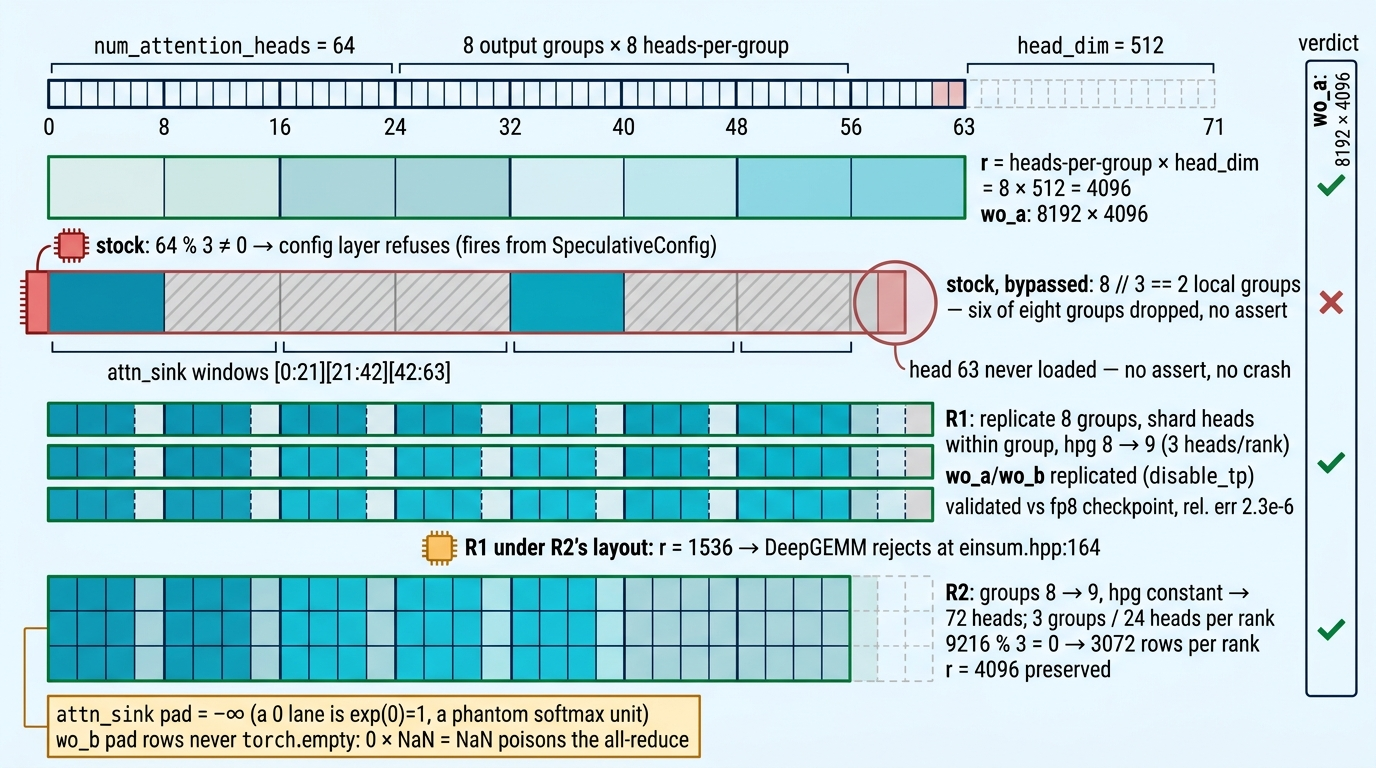
\includegraphics[width=\textwidth]{figures/ch12-shard-layouts.png}
\caption{Four ways to shard 64 heads across three ranks, judged by one
invariant. Stock refuses at the config layer ($64 \,\%\, 3 \neq 0$) and, if
bypassed, silently computes \code{8 // 3 == 2} local groups while its
\code{attn_sink} loader windows $[0{:}21][21{:}42][42{:}63]$ leave head~63
unloaded on every rank --- no assert, no crash, a healthy endpoint serving a
wrong model. R1 replicates the groups and shards heads within them, keeping
\code{wo_a}/\code{wo_b} replicated; it reproduces TP=1 output at
$2.3\times10^{-6}$ relative error under \emph{its own} layout, but its
3~heads-per-group would give $r = 1536$ under R2's sharded layout, which
DeepGEMM rejects at \code{einsum.hpp:164}. R2 pads the group count
$8 \to 9$ at constant heads-per-group, preserving the \code{o_proj}
contraction at $r = 4096$. A padding scheme is valid only relative to a
shard layout.}
\label{fig:tp3-shard-layouts}
\end{figure}

\begin{hblesson}
Pad lanes are not all equal. \repofile{dsv4_tp_pad.py}'s
\code{pad_fill_value} returns 0.0 for every parameter \emph{except}
\code{attn_sink}, which must be $-\infty$. The sink is an extra logit in the
softmax denominator: a zero pad lane contributes $\exp(0)=1$, a phantom unit
that attenuates every real attention weight --- ``plausible output, wrong
attention temperature.'' And \code{wo_b} pad rows must never be uninitialized
\code{torch.empty} memory, because $0 \times \mathrm{NaN} = \mathrm{NaN}$
poisons every rank through the all-reduce. Both TP-pad generations state this
independently; it is the most repeatable numerical-correctness lesson in the
patch corpus (\Cref{ch:patches}).
\end{hblesson}

The patcher applies eleven anchored edits, and their spread shows how deep a
``simple'' geometry change reaches. They include the config-layer
divisibility check (the actual boot blocker --- it fires from
\code{SpeculativeConfig} before any model class exists); three pad-aware
weight loaders in \repofile{parameter.py} that clamp the checkpoint copy to
what exists and zero-fill the tail --- with a documented replication trap
where offsetting a replicated parameter by \code{tp_rank} would silently
zero it on ranks $\ge 1$; MoE intermediate size $2048 \to 2112$ (a multiple
of $\mathrm{lcm}(3,64)=192$, so each rank's 704 columns stay 64-aligned for
NVFP4); vocab padding $129{,}280 \to 129{,}408$;
and the \code{attn_sink} loader windows that fix the silent head-63 drop
above.

\begin{hbwarstory}
The TP=3 patcher's idempotence markers originally hashed the patch
\emph{description}. When the patch body changed, a container whose writable
layer held the old patched file still looked ``already patched'' --- and that
layer survives every \code{docker compose restart} (restart is not recreate).
The only symptom was a shape assert on rank~2. The patcher now embeds a
SHA-256 prefix of the replacement body in each marker. A stale body yields
\code{STALE}, a hard exit-1 whose remediation is explicit: \code{docker rm -f}
on every node, because the anchor text was consumed and the file cannot be
re-anchored in place. \code{MISS} is equally fatal --- ``an unpatched
attn\_sink loader fails SILENTLY.''
\end{hbwarstory}

\subsection{One launcher per topology}

Three Sparks get a separate launcher, \repofile{start-tp3.sh}, and the reason
is stated in \repofile{docs/TP3.md}: a \envvar{TP_SIZE=3} line in
\repofile{.env.dspark} must not be able to silently change the two-node path.
The wrapper requires both \envvar{WORKER_HOST} and \envvar{WORKER2_HOST},
hard-fails if the patch file is missing, exports \envvar{DSPARK_TP3=1},
\envvar{TP_SIZE=3}, \envvar{NNODES=3}, and \code{exec}s the standard
launcher. Concurrency is likewise namespaced: \envvar{TP3_MAX_NUM_SEQS}
(or \code{--max-num-seqs 16}) is honored only by the TP=3 wrapper and ignored
by the two-node start, so an experiment's knobs cannot leak into the
production lane. One detail is quietly ahead of its sibling: the TP=3 usage
text documents CUDA-graph capture size as
$N \times (\text{MTP\_NUM\_TOKENS}+1)$ \emph{rounded up to a multiple of 8}
--- exactly the rounding whose absence on the TP=2 lane left the $c{=}6$
decode shape uncaptured (\Cref{ch:perf}).

\subsection{Bootstrapping the ring}

On a QSFP ring the third Spark is not on the spark1$\leftrightarrow$spark2
subnet: each pairwise link carries its own /24 (head
\code{10.0.22.1}$\,\leftrightarrow\,$\code{10.0.22.2} to spark2;
\code{10.0.23.1}$\,\leftrightarrow\,$\code{10.0.23.3} to spark3). That breaks
three assumptions the two-node fabric setup (\Cref{ch:fabric}) never had to
question, and the launcher rewires all three:

\begin{itemize}
\item \textbf{Bootstrap moves to the LAN.} Gloo, the NCCL socket, and the TP
TCP store move onto \envvar{TP3_BOOTSTRAP_IFNAME} (default \code{enP7s7})
--- the one network all three nodes share, and never \code{lo}, where Gloo
binds \code{127.0.0.1} and the mesh fails.
\item \textbf{Both head HCAs.} \envvar{NCCL_IB_HCA} is set to
\code{rocep1s0f0,rocep1s0f1} so spark1 faces both links (a single facing
HCA times out in QP RTR). And spark3's \envvar{WORKER2_NCCL_*} must be
pinned to its own port facing spark1, not copied from
\envvar{WORKER_NCCL_*}.
\item \textbf{Subnet-aware GID pairing.} The launcher disables NIC merging
(\envvar{NCCL_IB_MERGE_NICS=0}), enables subnet-aware routing, and sets
\envvar{NCCL_IB_SUBNET_PREFIX_LEN=24}: the default /16 would treat both /24s
as one subnet and pair GIDs across links that cannot reach each other.
\end{itemize}

\needspace{9\baselineskip}
\begin{lstlisting}[language=bash]
# .env.dspark additions for the third Spark (docs/TP3.md)
WORKER2_HOST=10.0.0.3
WORKER2_VLLM_HOST_IP=10.0.0.3
WORKER2_NFS_SERVER_IP=10.0.23.1   # head IP on the spark1<->spark3 link
WORKER2_NCCL_IB_HCA=rocep1s0f1    # spark3's port FACING the head
WORKER2_NCCL_SOCKET_IFNAME=enp1s0f1np1
WORKER2_TP_SOCKET_IFNAME=enp1s0f1np1
WORKER2_GLOO_SOCKET_IFNAME=enp1s0f1np1

./prepare-dspark-model-cache.sh --yes
./start-tp3.sh --max-num-seqs 16
scripts/validate_tp3.sh 127.0.0.1:8888   # prove the shard, not just HTTP
\end{lstlisting}

\begin{figure}[htbp]
\centering
\begin{tikzpicture}[node distance=10mm and 14mm]
  % nodes
  \node[hbhost, minimum width=34mm] (s1)
    {\textbf{spark1 (head)}\\rank 0 \(\cdot\) NFS exporter\\rocep1s0f0 + rocep1s0f1};
  \node[hbhost, below left=16mm and 8mm of s1, minimum width=30mm] (s2)
    {\textbf{spark2}\\rank 1\\mounts 10.0.22.1};
  \node[hbhost, below right=16mm and 8mm of s1, minimum width=30mm] (s3)
    {\textbf{spark3}\\rank 2\\mounts 10.0.23.1};
  % QSFP links
  \draw[hbarrow, <->, very thick] (s1.south west) -- (s2.north)
    node[hblabel, midway, left=2mm, align=right] {QSFP\\10.0.22.0/24};
  \draw[hbarrow, <->, very thick] (s1.south east) -- (s3.north)
    node[hblabel, midway, right=2mm, align=left] {QSFP\\10.0.23.0/24};
  \draw[hbarrow, <->, dashed, color=hbSteel!60] (s2.east) -- (s3.west)
    node[hblabel, pos=0.25, above=1mm, fill=white, inner sep=1pt] {ring segment};
  % NFS flows
  \draw[hbflow, bend right=28] (s1.west) to
    node[hblabel, above left=0mm and 1mm] {NFS ro} (s2.north west);
  \draw[hbflow, bend left=28] (s1.east) to
    node[hblabel, above right=0mm and 1mm] {NFS ro} (s3.north east);
  % LAN bus
  \coordinate (lanl) at ($(s2.south)+(-6mm,-9mm)$);
  \coordinate (lanr) at ($(s3.south)+(6mm,-9mm)$);
  \draw[very thick, color=hbGreen!70!black] (lanl) -- (lanr)
    node[hblabel, midway, below=1mm, color=hbGreen!70!black]
    {LAN enP7s7 \(\cdot\) 192.168.1.0/24 --- Gloo bootstrap, NCCL socket, TP TCP};
  \draw[hbok] (s2.south) -- ($(s2.south)+(0,-9mm)$);
  \draw[hbok] (s3.south) -- ($(s3.south)+(0,-9mm)$);
  \draw[hbok] (s1.south) .. controls +(0,-14mm) and +(0,10mm) ..
    ($(lanl)!0.5!(lanr)$);
  % NCCL knob annotation
  \node[hbpatch, right=6mm of s1, align=left, font=\scriptsize] (knobs)
    {NCCL\_IB\_MERGE\_NICS=0\\NCCL\_IB\_SUBNET\_AWARE\_ROUTING=1\\NCCL\_IB\_SUBNET\_PREFIX\_LEN=24};
  \draw[hbarrow, dashed] (knobs.west) -- (s1.east);
\end{tikzpicture}
\caption{TP=3 on the QSFP ring. Each pairwise link is its own /24, so NCCL
needs both head HCAs and /24-aware GID pairing; process-group bootstrap rides
the shared LAN, never \code{lo}. Worker~2 mounts the head's HF cache at the
head's address \emph{on its own link} (10.0.23.1), which the start script
grants to the live NFS exporter.}
\label{fig:tp3-ring}
\end{figure}

The launcher checks --- but does not perform --- the third node's
prerequisites: passwordless SSH, and the pinned $\approx$19\,GB vLLM image
already pulled (it refuses to boot and prints the exact \code{docker pull}
command otherwise). With \envvar{DSPARK_WORKER_HF_NFS=1} it syncs compose,
env, and \repofile{patches/tp3/}, and mounts the head's HF cache over NFS, so
spark3 needs no local checkpoint.

\subsection{What three nodes buy --- and what they cost}

\Cref{tab:tp3-ledger} is the repository's own warm A/B (2026-09-02, same image,
prose prompts, 512 output tokens; TP=3 at 16 slots vs TP=2 at 6).

\begin{table}[htbp]
\centering\small
\caption{The TP=3 ledger (\repofile{docs/TP3.md}, reference cluster).}
\label{tab:tp3-ledger}
\begin{tabular}{lll}
\toprule
Load & TP=2 & TP=3 \\
\midrule
decode, 1 stream & 38.6 \tokspersec{} & 41.9 \tokspersec{} (+9\,\%) \\
decode, 2 streams & 63.9 agg & 72.0 agg (+13\,\%) \\
decode, 4 streams & 86.0 agg & 89.7 agg (+4\,\%) \\
decode, 8 / 12 / 16 streams & n/a (6 slots) & 142.8 / 164.3 / 198.0 agg \\
TTFT 8k / 16k / 32k / 64k & 4.4 / 8.7 / 18.0 / 36.0 s & +4--13\,\% slower \\
TTFT 128k / 256k & 74.9 / 164.8 s & 91.5 / 202.2 s (+22--23\,\%) \\
KV cache per rank & $\approx$16.8 / 15\,GiB & $\approx$35 / 34 / 35\,GiB \\
\bottomrule
\end{tabular}
\end{table}

The headline: 16 slots, $\approx$5.0M KV tokens ($4.8\times$ concurrency at
1M), $\approx$200 \tokspersec{} aggregate at $c{=}16$, and modestly faster
per-stream decode (+4--13\,\%) --- against prefill that is 4--23\,\%
\emph{slower}, worst at $\ge$128k. The ``why'' is architectural, not
incidental. In DeepSeek's MLA every rank holds the full latent KV and the
Lightning indexer is replicated (\Cref{ch:architecture}), so the attention
share of prefill does not shrink with a third GPU. Meanwhile the pad (heads
$64 \to 72$) adds real work, and a three-rank ring all-reduce over two
different physical links costs roughly twice the latency of a two-rank
exchange.

The audit's first-principles model (\Cref{ch:perf}) makes the same
point from the decode side: bytes per rank per step drop from
$\approx$16.5\,GB to $\approx$11.5\,GB, yet the measured step barely
moves.
Bandwidth arithmetic alone predicts a $\approx$48\,ms step from those
11.5\,GB; the measured step is $\approx$61\,ms --- roughly 13\,ms of fixed
per-step cost, and the bandwidth gain is gone. That single measurement is
the mechanism behind the chapter's opening headline: the fixed overheads a
third rank adds --- a three-rank ring over two different physical links,
the padded heads' extra work --- are exactly what the unshrinkable
attention share of prefill pays at 128k--256k, surfacing as the +22\,\%
TTFT regression. TP=3 is a capacity trade; single-user long-context work
stays on the two-node lane.

\begin{hbnote}
First boot at TP=3 is slow by design, not broken. Spark3 starts with an empty
JIT cache and the TP=3 shard shapes are new for all three nodes, so the first
\repofile{start-tp3.sh} spends several minutes compiling ($\approx$8 minutes
to healthy on the reference pair; engine init alone 193\,s). The first
requests still hit Triton JIT spikes. Do not restart a boot that is merely
compiling --- wait for \code{HEALTH_OK} / \code{boot-shape-warmup}. Later
boots reuse the persisted caches.
\end{hbnote}

\section{The Stage-C lane: 200K $\times$ 16}

The second scaling path changes the \emph{runtime}, not the node count. The
default serve lane patches the pinned Anemll image at container start
(\Cref{ch:patches}). The \repofile{recipe/} lineage instead bakes the
$\approx$20 DSpark overlay source files over a different base ---
\repofile{ghcr.io/bjk110/vllm-spark:unholy-fusion-prod-ready}, the
``unholy fusion'' GB10 build carrying the B12X MoE kernels --- with a
\code{py_compile} gate at build time. On top of that clean overlay sit three
NVFP4 stages whose names tell the story of a probe and a retreat:

\begin{description}
\item[Stage A --- the dtype exists.] Registers \code{nvfp4_ds_mla} in
\code{CacheDType}, maps it to \code{torch.uint8} and
\code{KVQuantMode.NVFP4}, and gives the KV interface a real-page-size branch
at 416 bytes per token.
\item[Stage B --- the 416\,B probe.] Teaches the DeepSeek-V4 attention layer
to accept the dtype with \code{head_bytes = 416} --- the GLM-5.2 NVFP4
sparse-MLA per-token record --- to probe whether DSV4's store/decode kernels
are compatible with the GLM record. They are not, yet.
\item[Stage C --- retreat to the known envelope.] \sloppy Rewrites the
416-byte cells back to DeepSeek V4's proven \textbf{584-byte} envelope for
\code{nvfp4_ds_mla}, model-version-gated. The in-line rationale: keep the
hybrid MLA/SWA grouping bootable first (``padded NVFP4 probe''); kernel and
store correctness is the next experiment.
\end{description}

Stage C is where the \envvar{VLLM_DSPARK_*} tuning family actually exists.
On the Anemll 0.1.1 image those keys are unregistered and produce only
``Unknown vLLM environment variable'' warnings ---
\repofile{docker-compose.stage-c.override.yml} is inert there by design. The
one that matters most for scale is
\envvar{VLLM_DSPARK_GPU_REJECTED_CONTEXT_MASK=1}, the ragged-batch path
required once the Keys concurrency patch (request-stable draft-KV slots,
\Cref{ch:specdecode}) unlocks \code{max_num_seqs > 1} with mixed
prefill+decode batches.

The measured lane --- Stage-C image, \code{max_model_len=200000},
\code{max_num_seqs=16}, Keys patch at \code{7e4d94bb} --- is summarized in
\Cref{tab:stagec-lane}.

\begin{table}[htbp]
\centering\small
\caption{The Stage-C lane, measured (aggregate \tokspersec{}; per-stream and
acceptance in parentheses).}
\label{tab:stagec-lane}
\begin{tabular}{@{}llll@{}}
\toprule
Arrivals & $c{=}1$ & $c{=}8$ & $c{=}16$ \\
\midrule
static & 57.6 (acc.\ 0.635) & 252.6 (31.6/stream) &
\textbf{315.1} (19.7/stream, 0.609) \\
staggered & --- & --- & 205.0 \\
\bottomrule
\end{tabular}
\end{table}

The repository's own caveat deserves
repeating verbatim in spirit: this is a \emph{short-context, high-aggregate}
profile --- a different product than the 1M-context agent lane, not a faster
version of it.

\section{Horizontal scale-out: replicas behind a router}

Both paths so far change the engine --- its shard geometry or its runtime
image. The least glamorous path changes neither, and it is the one
\repofile{docs/SETUP.md} actually ran:
four Sparks as \emph{two independent TP=2 replicas} serving the same
DeepSeek-V4-Flash-DSpark checkpoint. Replica A was the control --- the
Rafael Caricio stack, unpatched, pinned at \code{max-num-seqs=1}, holding
$\approx$52--54 \tokspersec{} single-stream throughout. Replica B ran the
packaged recipe with the Keys concurrency patch and swept
\code{max-num-seqs} from 1 to 16, so every concurrency claim in the recipe
was measured against a live unpatched baseline on identical hardware,
serving at the same time. The experiment's shape is as instructive as its
numbers: nothing about a second pair required new numerics, new fabric
work, or a new launcher --- replica B could be patched, swept, and rolled
back while replica A kept serving.

That layout generalizes into SETUP.md's final step: run a second patched
TP=2 replica and put a least-connections router in front for roughly
$2\times$ aggregate throughput and concurrency. Because replicas share
nothing at runtime, this path has none of TP=3's numerics or fabric risk
--- and none of its KV-pool consolidation either. Each replica keeps its
own $\approx$2.3M-token pool, and a request sees only its replica's cache.
Where the workload is many independent sessions rather than one giant
context, the router is the better trade (\Cref{fig:kv-two-ways} draws the
three capacity paths against what a single request can actually reach); the
two lanes compose, since each replica could itself be a TP=3 triple.

\begin{figure}[htbp]
\centering
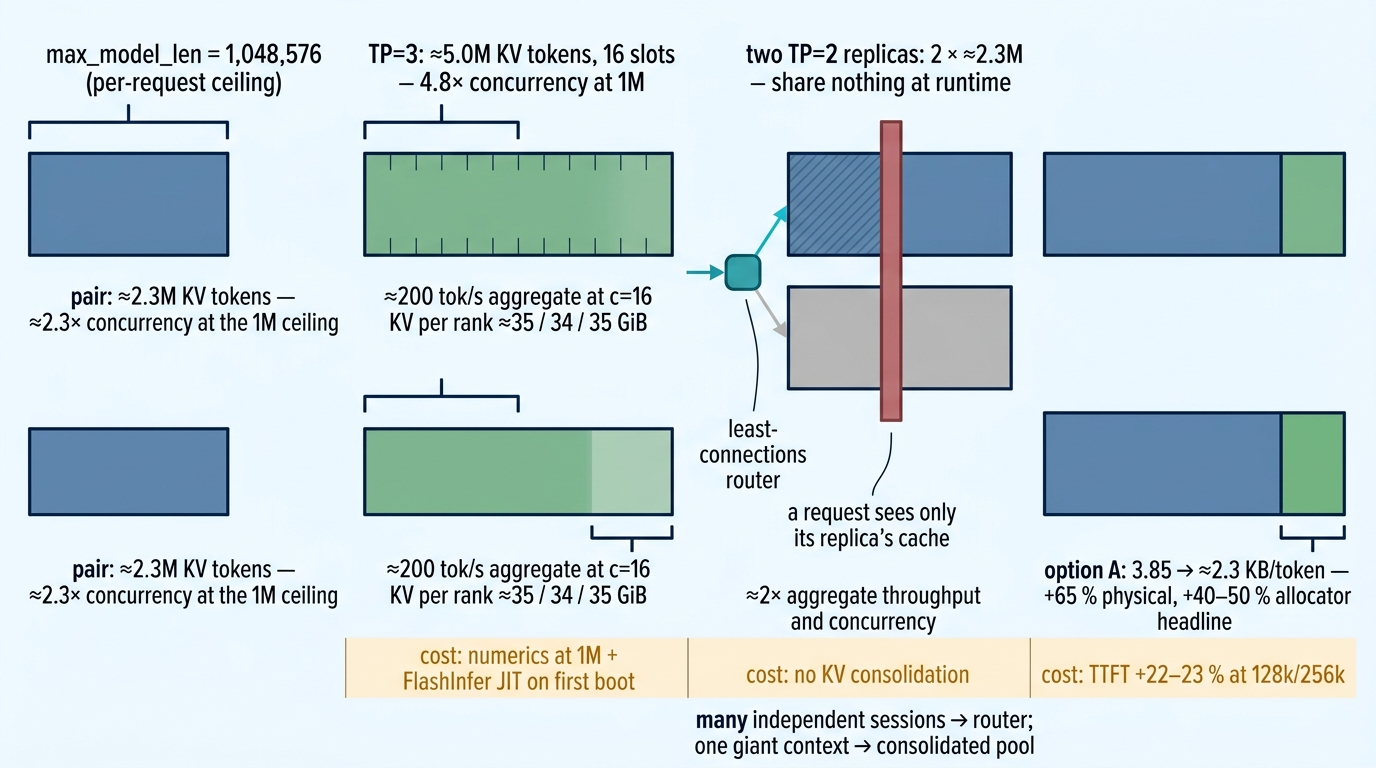
\includegraphics[width=\textwidth]{figures/ch12-two-ways-kv.png}
\caption{More KV is not one thing. TP=3 consolidates into a single
$\approx$5.0M-token pool ($4.8\times$ concurrency at the 1M ceiling, 16
slots) that one request can draw from --- paid for with prefill 4--23\,\%
slower and TTFT +22--23\,\% at 128k--256k. Two TP=2 replicas behind a
least-connections router give $\approx 2\times$ aggregate throughput with
none of TP=3's numerics or fabric risk, but they share nothing at runtime:
each keeps its own $\approx$2.3M-token pool and a request sees only its
replica's cache. Item-8's option-A row grows the existing pool in place
instead, $\approx$3.85 $\to$ $\approx$2.3\,KB per token. The lanes compose
--- each replica could itself be a TP=3 triple.}
\label{fig:kv-two-ways}
\end{figure}

\section{Weights logistics at scale}

Every extra node multiplies a mundane problem: the checkpoint is hundreds of
gigabytes, and the abliterated variant nearly doubles it if copied naively.

\subsection{NFS mode: one copy of the weights}

With \envvar{DSPARK_WORKER_HF_NFS=1}, workers keep no local checkpoint. The
head exports its HuggingFace cache read-only over the ConnectX fabric from a
privileged Alpine container running a \emph{kernel} NFSv4-only server
(\repofile{files/nfs-server/}): the entrypoint mounts \code{nfsd} and
\code{rpc_pipefs}, generates \repofile{/etc/exports} with one line per
client, then runs \code{rpc.nfsd 8}. Two design points carry the operational
weight:

\begin{itemize}
\item \textbf{Live-exporter reuse.} \code{nfs_ensure_server} first probes
\code{rpcinfo -t $ip nfs 4}; if \emph{any} NFSv4 server already answers
(the Qwen recipe's \code{vllm-fn-nfs}, or a previous \code{dspark-nfs}), it
is reused rather than duplicated. The comment explains why: kernel nfsd in a
privileged container can leave rpcbind in D-state, and then
\code{docker rm -f} hangs --- ``do not docker rm a working share.'' For the
third node, \code{nfs_grant_subnet} appends the new /24 to the \emph{running}
exporter's exports and re-runs \code{exportfs -rav}, without recreating a
container another recipe may be using. Teardown
(\repofile{stop-deepseek-v4-flash-dspark.sh}~\code{--nfs}) removes only the
DSpark-owned exporter, never \code{vllm-fn-nfs}.
\item \textbf{Read-only weights, writable JIT.} The worker mounts the named
volume \code{dspark-hf} (\code{nfsvers=4.2,ro,nconnect=8}, 1\,MiB
rsize/wsize, \code{hard,timeo=600}) in place of the host HF bind. The
override compose overlays \emph{six local writable bind mounts} on top of the
read-only tree --- \code{triton-cache}, \code{tilelang-cache},
\code{vllm-cache}, \code{flashinfer}, \code{b12x-cute-cache},
\code{nccl-fr}. Compiled-kernel caches must be per-node and writable while
weights stream read-only from one copy; the head pre-creates the mount-point
directories because overlay points must already exist on a read-only export.
\end{itemize}

\subsection{The 26-shard abliterated overlay}
\label{sec:scale-ablit-overlay}

The abliterated Vision-Exp variant edits only layers 10--35
\code{attn.wo_b} --- 26 tensors packed in shards 00012--00037.
\repofile{scripts/overlay-vision-exp-ablit-cache.py} exploits that:
it classifies blobs shared between the official and abliterated snapshots,
\emph{hardlinks} the shared ones into the abliterated repository's blob store,
copies (or rsyncs to the worker, via a \code{--files-from} list) only the
unique shards, and rebuilds the snapshot symlink tree. A manifest mode
exports the classification as JSON so a node without the source cache can
verify ``unique ablit blobs missing ($N$)'' and fail with the list. Two
near-identical multi-hundred-GB models cost one checkpoint plus 26 shards.

\section{KV persistence: LMCache}

Shared storage settles where the weights live; it does nothing for the
other large state a restart destroys. Restarting the engine normally
forfeits every cached context; at 1M-class
contexts that is minutes of re-prefill per session. The experimental
\repofile{lmcache/} option keeps KV in per-node \code{lmcache server}
processes (L1 in CPU RAM, filesystem L2 on local NVMe) that survive engine
restarts, wired in through \code{LMCacheMPConnector} over ZMQ on the fabric
IPs. The measured win is dramatic: a $\approx$107K-token context that costs
$\approx$65\,s to re-prefill reloads in \textbf{1.8--1.9\,s} (measured
$n{=}2$, GB10 pair, \code{nvfp4_ds_mla}). What that reload costs is
structural rather than numerical: the KV outlives the engine precisely
because it now lives in a process the engine's own lifecycle does not own,
and each failure mode below follows from that single fact.

The README then spends most of its length on why you might \emph{not} turn it
on, under an explicit ``owner decision required'' heading. Three named
failure modes:

\begin{enumerate}
\item \textbf{The servers live outside Compose.} They are plain
\code{docker run} containers --- not started, stopped, health-checked, or
supervised with the model containers --- and the stop script
(\repofile{stop-deepseek-v4-flash-dspark.sh}) leaves them running. Boot order
is manual and load-bearing: every node's server must be up \emph{and
verified} before the engine starts.
\item \textbf{Confirmed unified-memory cold-boot OOM.} On 128\,GB
unified-memory boards the kernel OOM killer has killed the server during an
engine cold boot --- the weight-load spike lands on top of the server's
resident L1 (confirmed in \code{dmesg}; reported upstream as LMCache \#4759).
Mitigations: size L1 down, and optionally set \envvar{LMCACHE_OOM_SCORE_ADJ}
negative so the killer prefers the Compose-restarted engine over the
unsupervised server. The recipe deliberately defaults that knob to 0,
because it is a node-wide policy choice ``not ours to make.''
\item \textbf{A dead server wedges the engine --- silently.} A restarted or
killed server loses its GPU contexts; current upstream code then parks every
lookup-hit request forever. The scheduler heartbeat never starts, so dead
servers stay ``healthy''; lookup errors do not propagate; the engine neither
crashes nor falls back to re-prefill. An operator watching container exits
sees a healthy pair serving nothing.
\end{enumerate}

\begin{hbwarning}
Failure mode 3 dictates the restart-order doctrine. Servers run with
\code{--restart no} --- a dead server must stay dead and \emph{visible}.
The launcher refuses to recreate a server while any \code{vllm-dspark}
container is live, because a fresh server under a live engine \emph{is} the
wedge. The only supported recovery is a full-pair restart, servers first,
then the engine. Moving the servers into Compose is deliberately out of
scope: Compose auto-restarting an emptied server is exactly the wedge. Until
LMCache PR \#4764 (heartbeat) lands, the blast radius of a dead cache server
is the model service.
\end{hbwarning}

Two configuration invariants are non-negotiable: \envvar{PYTHONHASHSEED=0} on
every process (chunk keys use Python's randomized \code{hash()}; unpinned,
every restart invalidates the whole cache --- LMCache \#1788), and L1 sized
to the largest context (\code{--l1-size-gb 12} for $\approx$150K-token
documents; mid-store L1 eviction has stalled stores). The compose patcher
puts every LMCache delta inside one entrypoint branch gated on
\envvar{DSPARK_ENABLE_LMCACHE} being exactly \code{1}, so a single compose
file serves both modes and the off state is verifiably stock.

\begin{lstlisting}[language=bash]
# one server per node, bound to THAT node's fabric IP; both must verify
./lmcache/run-lmcache-server.sh 192.168.104.10   # head
./lmcache/run-lmcache-server.sh 192.168.104.11   # worker
python3 lmcache/patch-compose-lmcache.py \
  docker-compose.dspark.yml docker-compose.lmcache.yml \
  tcp://192.168.104.10:6667,tcp://192.168.104.11:6667
export DSPARK_ENABLE_LMCACHE=1
COMPOSE_FILE=$PWD/docker-compose.lmcache.yml ./start-deepseek-v4-flash-dspark.sh
\end{lstlisting}

\begin{figure}[htbp]
\centering
\adjustbox{max width=\textwidth}{%
\begin{tikzpicture}[node distance=6mm and 10mm]
  % head node group
  \node[hbgpu, minimum width=30mm] (eng) {vLLM engine\\(vllm-dspark, rank 0)};
  \node[hbnode, right=34mm of eng, minimum width=30mm] (srv)
    {lmcache server\\L1: 12\,GB CPU RAM};
  \node[hbhost, below=of srv, minimum width=30mm] (l2) {L2: local NVMe\\(fs adapter)};
  \node[hbfaint, below=of eng, minimum width=30mm] (worker)
    {worker node:\\same pair, mirrored};
  \begin{scope}[on background layer]
    \node[hbgroup, fit=(eng)(worker), label={[hbtitle]above:Compose lifecycle}] (grp) {};
  \end{scope}
  \draw[hbflow, <->] (eng) -- (srv)
    node[hblabel, pos=0.55, above=0.5mm, font=\tiny] {ZMQ tcp://fabric-ip:6667};
  \draw[hbarrow, <->] (srv) -- (l2);
  % failure-mode annotations
  \node[hbwarn, right=12mm of srv, align=left, font=\scriptsize] (f1)
    {F1: outside Compose ---\\manual, load-bearing\\boot order};
  \node[hbwarn, below=4mm of f1, align=left, font=\scriptsize] (f2)
    {F2: cold-boot OOM ---\\weight-load spike +\\resident L1 (dmesg)};
  \node[hbwarn, below=4mm of f2, align=left, font=\scriptsize] (f3)
    {F3: dead server parks\\lookup hits forever ---\\engine wedges silently};
  \draw[hbfail] (f1.west) -- (srv.north east);
  \draw[hbfail] (f2.west) -- (srv.east);
  \draw[hbfail] (f3.south) to[bend left=25] (worker.east);
  % doctrine
  \node[hblabel, below=4mm of worker, align=center]
    {-{}-restart no \(\cdot\) servers up before engine \(\cdot\)\\
     recovery = full-pair restart, servers first};
\end{tikzpicture}%
}
\caption{LMCache on the pair: per-node cache servers outside the Compose
lifecycle, ZMQ on the fabric IPs, L1 RAM + L2 NVMe. The three named failure
modes (red) are why enabling it is framed as an owner decision, not a free
$65\,\mathrm{s} \to 1.9\,\mathrm{s}$ win.}
\label{fig:lmcache-arch}
\end{figure}

\section{The 4-bit KV future}

LMCache stretches the KV pool across restarts; the last path stretches it
in place, and it is the deepest: making the cache row actually 4-bit. It is
also the path whose binding constraint sits somewhere other than intuition
puts it --- not how few bits attention can tolerate, but which row sizes the
hybrid KV allocator's uniform page will accept --- so the arithmetic that
follows is a search for a divisor as much as for a precision. Today
\code{nvfp4_ds_mla} is byte-identical to \code{fp8_ds_mla} --- 584 bytes per
token: 448\,B of fp8 e4m3 NoPE with seven UE8M0 per-64 scales, 128\,B of
bf16 RoPE, and an 8-byte footer. The ``nvfp4'' string changes only kernel
dispatch (which is why issue \ghissue{22} routed it to the fp8 kernel).
\repofile{docs/CLAUDE/item8-fp4-kv-design.md} is the design study for a real
compressed row. Its central constraint comes from vLLM's hybrid KV
allocator: every KV group --- 1 MLA plus 3 sliding-window groups --- must
share the same page size in bytes, today $64 \times 584 = 37{,}376$\,B. Only
row sizes that divide that page with a power-of-two row count are cheap:
$584 \times 64 = 292 \times 128 = 146 \times 256$. That arithmetic sorts the
options (\Cref{tab:fp4-options}).

\begin{table}[htbp]
\centering\footnotesize
\caption{Item-8 layout options for the compressed (C4/C128) row against the
uniform-page constraint.}
\label{tab:fp4-options}
\begin{tabular}{>{\raggedright\arraybackslash}p{2.6cm}>{\raggedright\arraybackslash}p{3.6cm}p{1.4cm}p{1.3cm}>{\raggedright\arraybackslash}p{3.4cm}}
\toprule
Option & Row & Bytes & Fits page? & Risk / cost \\
\midrule
A --- half row & e2m1 NoPE + 4 UE8M0 scales per 128 + fp8 RoPE &
292 & yes (exact) & block-128 scaling coarse for e2m1; one quant-tile change \\
B --- fp4 RoPE & MXFP4 NoPE (per-32) + e2m1 RoPE & 280/292 & yes &
positional precision at 1M --- highest quality risk \\
C --- keep bf16 RoPE & 224 + 14 + 128\,B RoPE & 366$\to$368 & \textbf{no} &
needs per-group page sizes (upstream allocator change); SWA row is written by
a C++ op \\
D --- DCP-2, no fp4 & keep 584\,B; shard \emph{tokens} across ranks & --- &
n/a & zero numerics risk; DSV4 sparse backend has no DCP in this image \\
\bottomrule
\end{tabular}
\end{table}

The recommendation is to prototype \textbf{option A} first: it fits the page
exactly at 292 bytes, preserves RoPE at fp8, and changes one quantization
tile. Expected capacity: the compressed per-token term drops from 3.07 to
1.54\,KB, total physical bytes from $\approx$3.85 to $\approx$2.3\,KB/token
--- \textbf{+65\,\% tokens at the physical level}, +40--50\,\% in the
allocator headline (the SWA groups keep 584-byte pages). The study is candid
that the headline ``2.33M tokens in 17.04\,GiB'' is allocator accounting
across four groups, not physical row cost --- which is exactly why shrinking
the compressed row moves capacity more than linearly.

\begin{figure}[htbp]
\centering
\begin{tikzpicture}
  % scale: 0.021 cm per byte
  % Row 1: 584 B  (448 | 128 | 8)
  \node[hbtitle, anchor=south west] at (0,1.05) {today: 584 B/token
    (\,fp8\_ds\_mla \(=\) nvfp4\_ds\_mla\,)};
  \draw[fill=hbBlue!10, draw=hbSteel, thick] (0,0) rectangle (9.41,0.9);
  \node[font=\scriptsize] at (4.7,0.45)
    {NoPE 448 B --- fp8 e4m3, 7 UE8M0 scales per 64 dims};
  \draw[fill=hbGreen!12, draw=hbSteel, thick] (9.41,0) rectangle (12.10,0.9);
  \node[font=\scriptsize, align=center] at (10.75,0.45) {RoPE 128 B\\(64 \(\times\) bf16)};
  \draw[fill=hbAmber!35, draw=hbSteel, thick] (12.10,0) rectangle (12.27,0.9);
  \node[hblabel, anchor=north east, font=\tiny] (foot) at (12.27,-0.12) {footer 8 B (7 scales + pad)};
  \draw[hbarrow] (foot.north) -- (12.18,-0.02);
  % Row 2: 292 B  (224 | 4 | 64)
  \node[hbtitle, anchor=south west] at (0,-1.35) {option A: 292 B/token
    (proposed nvfp4c\_ds\_mla)};
  \draw[fill=hbBlue!10, draw=hbSteel, thick] (0,-2.4) rectangle (4.70,-1.5);
  \node[font=\scriptsize] at (2.35,-1.95) {NoPE 224 B --- e2m1 (2/byte)};
  \draw[fill=hbAmber!35, draw=hbSteel, thick] (4.70,-2.4) rectangle (4.79,-1.5);
  \draw[fill=hbGreen!12, draw=hbSteel, thick] (4.79,-2.4) rectangle (6.13,-1.5);
  \node[hblabel, anchor=west] (sc) at (6.6,-1.7) {4 \(\times\) UE8M0 per-128 (4 B)};
  \draw[hbarrow] (sc.west) -- (4.745,-1.52);
  \node[hblabel, anchor=west] (rp) at (6.6,-2.15) {RoPE 64 B (fp8)};
  \draw[hbarrow] (rp.west) -- (6.13,-1.95);
  % page arithmetic
  \node[hblabel, anchor=north west, align=left] at (0,-2.8)
    {same 37{,}376-byte page: 64 rows \(\times\) 584 B \(=\) 128 rows
     \(\times\) 292 B\\--- the hybrid allocator's uniform-page constraint,
     satisfied exactly};
\end{tikzpicture}
\caption{Byte map of the current 584\,B KV row versus item-8's proposed
292\,B option-A row, drawn to a common byte scale. Option A halves the row by
packing NoPE as e2m1 with coarser per-128 scales and quantizing RoPE to fp8;
the footer's role is absorbed by the four scale bytes.}
\label{fig:kv-bytemap}
\end{figure}

\begin{sloppypar}
The plan is staged to buy information cheaply: a one-line probe, then a
2--3-week fork, with DCP as the no-numerics exit. \textbf{Step 0} costs
almost nothing: vLLM already ships an MXFP4 \emph{indexer} K cache, gated to
datacenter Blackwell at \code{indexer.py:274-283} --- but DeepGEMM ships
\code{sm120_fp4_*} logits headers, so the gate is probably conservative
rather than a kernel limit. A one-line relaxation plus
\code{--attention-config} would halve the replicated indexer cache
($-0.35$\,KB/token $\approx -9\,\%$ of KV bytes) and halve indexer K reads.
It requires the SM121 DeepGEMM header-alias hotfix, because the fp4 kernels
are certainly not in the JIT cache yet.

The full option-A fork is estimated at 2--3 engineer-weeks: offline
numerics first (dump real compressed rows, simulate the quant/dequant in
numpy --- the Stage-C knob
\envvar{VLLM_DSPARK_REFERENCE_KV_QUANT_DEQUANT} was built for exactly this
kind of check), then an fp4 writer variant under a \emph{new} dtype string
(\code{nvfp4c_ds_mla}, so \ghissue{22}'s meaning of \code{nvfp4_ds_mla} is
not broken), and a new FlashInfer \code{KVCacheTraits} with stride 292 and
a renamed JIT module to bust the cache.

Validation runs the instruments of \Cref{ch:measurement}: RULER-lite, the
garble sweep to 900K, and spec-decode acceptance. The named risks are
numerics at 1M context and minutes of FlashInfer JIT on first boot. Option
D --- decode-context parallelism instead of quantization --- remains the
zero-numerics alternative if upstream lands DSV4 DCP support.
\end{sloppypar}

\begin{hbnote}
A sibling artifact attacks 4-bit \emph{weights} rather than KV: the
\repofile{vllm_patch_gb10/} plugin's opt-in \code{modelopt_gb10_hybrid}
quantization method dispatches Marlin W4A16 below $M{=}128$ (latency-bound
decode) and CUTLASS W4A4 at or above it, at a documented
double-weight-memory cost --- and with the honest label that it was tested
``only for syntax packaging, not on a live GB10.''
\end{hbnote}

\begin{sloppypar}
The root \repofile{Dockerfile.gb10-dsv4-dspark} shows what
the endgame looks like when the base cooperates: on the newer vLLM~0.26 base
it commits to the \emph{true} packed 352\,B/token NVFP4 layout (256\,B E2M1
NoPE + 32\,B E4M3 block-16 scales + 64\,B fp8 RoPE), because that base ships
the real write kernel --- \code{concat_and_cache_nvfp4_ds_mla.cu},
kStride\,=\,352 --- and the FlashInfer SM120 backend to read it. It also
carries the \code{get_kv_cache_spec} dtype fix (uint8, not bf16), without
which the per-token stride silently doubles --- the same bug class as issue
\ghissue{22}.
\end{sloppypar}

Scaling has stopped being a dial and become a menu of asymmetric trades.
Every path buys one specific axis --- decode slots and KV pool, aggregate
throughput, survival across a restart, bytes per token --- and charges for
it in a different currency: numerics risk, prefill latency, an operational
wedge, or an allocator constraint that outranks the kernels entirely. What
decides which paths exist at all is architectural rather than economic:
whatever is replicated on every rank, MLA's latent KV and the Lightning
indexer above all, does not shrink when a rank is added, which is why the
honest verdict on a third GPU is a capacity lane and never a speed lane.

\FloatBarrier
\section*{Takeaways}

\begin{itemize}
\item TP must divide the attention-group count; when it does not, prefer a
loud pad to a silent \code{8 // 3 == 2}. A padding scheme is only valid
relative to a shard layout --- the \code{o_proj} einsum's
$r = \text{hpg} \times \text{head\_dim} = 4096$ contract, not divisibility,
decided between the R1 and R2 generations --- and pad values are semantics:
\code{attn_sink} pad lanes must be $-\infty$ (a zero lane is a phantom
softmax unit), and pad rows must never be uninitialized memory feeding an
all-reduce.
\item A third rank buys capacity, not speed. MLA replicates the latent KV
and the indexer on every rank, so the attention share of prefill does not
shrink, while the pad ($64 \to 72$ heads) and a three-rank ring all-reduce
over two physical links add work on top --- hence 16 slots and
$\approx$5.0M KV tokens against TTFT 22--23\,\% worse at 128k--256k. Two
TP=2 replicas behind a least-connections router are the shared-nothing
alternative: $\approx 2\times$ aggregate with none of the numerics or
fabric risk, and no shared KV pool either.
\item Quarantine every risky lane. \repofile{start-tp3.sh} and
\envvar{TP3_MAX_NUM_SEQS} exist so a stray \envvar{TP_SIZE=3} in
\repofile{.env.dspark} cannot flip the production two-node path; a new
topology also voids fabric assumptions, so bootstrap on the shared LAN,
enable both head HCAs, and make NCCL /24-aware
(\envvar{MERGE_NICS=0}, subnet-aware routing) --- the default /16 merges
links that cannot reach each other. The Stage A$\to$B$\to$C lineage is the
same instinct inside the runtime: make the dtype exist, probe the foreign
record, retreat to the proven envelope so the system stays bootable while
the next experiment is prepared.
\item Ship weights once: a read-only kernel-NFS export with per-node writable
JIT overlays, live-exporter reuse, and a hardlink overlay that pays for only
the 26 shards an abliterated variant actually changes.
\item State that outlives the engine is an operational contract, and the
allocator constrains the 4-bit future before the kernels do. LMCache's
$65\,\mathrm{s} \to 1.9\,\mathrm{s}$ reload comes with three named failure
modes and a servers-first restart doctrine, framed explicitly as an owner
decision; item-8's 292-byte row is recommended not because four bits
suffice but because $292 \times 128$ equals the existing page exactly,
promising +65\,\% physical capacity --- with a cheap MXFP4-indexer step 0
and DCP-2 as the zero-numerics fallback.
\end{itemize}

\chaptertransition{Twelve chapters of specifics --- a fabric, a scheduler, a
drafter, forty patches, six audit phases, six scaling paths --- earn their
pages only if something survives the model, the engine build, and the two
machines they were measured on. The final chapter extracts exactly that:
the principles stated as doctrine, each grounded in the incident that cost
enough to teach it. What the list is made of is the uncomfortable part ---
eight of eleven plausible performance knobs rejected, and the single most
consequential bug in the system a configuration field that existed,
defaulted sensibly, and was never read by anything that ran.}

\chapter{Lessons for Your Own Deployment}
\label{ch:lessons}

Of eleven plausible performance knobs A/B-tested on this cluster, eight were
rejected --- including several that ``obviously'' should have helped. The
single most consequential bug in the system was not a kernel fault or a
race but a configuration field that existed, defaulted sensibly, and was
never read. Results like these are why the closing chapter of this handbook
is not a victory lap: nearly every principle worth keeping was learned by
watching a reasonable assumption fail in a specific, documented way.

A handbook about one system earns its keep by what transfers out of it. This
closing chapter collects the principles the preceding twelve chapters
demonstrated in the concrete --- each stated as doctrine, grounded in the
incident that taught it, and phrased so it can be applied to a different
model, a different engine, and different hardware tomorrow.

For an inference engineer, this is the chapter meant to outlive its subject.
The specific patches are bound to one model, one engine build, and one pair
of machines; the disciplines --- pinned artifacts, fail-closed patching,
identity-keyed state, loud failure, public retraction --- are not. Each
one below carries the incident that proves what skipping it costs.

\section{Change nothing you cannot prove}

\subsection*{1. Pin everything; patch fail-closed}
The runtime image is pinned by manifest digest, the checkpoint by revision,
and every runtime modification by the SHA-256 of the bytes it expects to
find. A patch that cannot prove its target aborts the boot rather than
serving stock code under an enabled flag (\Cref{ch:patches}). The general
form: \emph{an optimization or fix that silently fails to apply is worse
than its absence}, because you will debug the system you believe you
deployed, not the one you did.

\subsection*{2. ``Defined but unenforced'' is a bug class, not a config style}
Pinning proves the bytes are present; it cannot prove a knob is connected
to anything. The starvation arrived with a clean bill of health: decode
lanes stalled behind prefill with zero preemptions and every dashboard
green. \code{max_num_partial_prefills} (\ghissue{27}) --- the cap that
should have bounded the damage --- was connected to nothing that ran. Audit the path
from every knob you rely on to the code that consumes it. The same family
produced the dead \code{IntEnum}-vs-string comparison found while auditing
\ghissue{55}.

\subsection*{3. Exactly-one spelling of ``on''}
Auditing knob-to-consumer paths is only tractable when the space of ``on''
is small. Every opt-in here is gated on the literal string \code{1}; every other value
--- \code{true}, \code{yes}, \code{2}, whitespace --- is stock. Combined with
default-off for anything unproven, this collapses the configuration state
space and makes ``what is this cluster running?'' answerable from one file
plus one rule (\Cref{ch:patches}).

\subsection*{4. Restart is not rollback}
One file plus one rule answers what the cluster is \emph{configured} to
run; what it is \emph{actually} running can still diverge.
Runtime patches live in the container's writable layer; flipping a flag off
and restarting reuses those bytes. Only recreation restores image truth ---
and the doctrine must be paired: \emph{both} ranks recreated together, never
one (\Cref{ch:operations}). Wherever you mutate a running artifact, write
down what actually reverts it, and test that path.

\section{Identity, capture, and blast radius}

The first four principles govern what you deploy; the next four govern how
it fails while serving --- and they escalate in scope, from one request's
state to the whole host.

\subsection*{5. Identity, not position}
Under continuous batching the engine condenses its running set; anything
keyed by \emph{batch row} silently reads another request's state after a
condense. DSpark's draft KV did exactly that, collapsing acceptance at
concurrency $>1$ with no crash (\Cref{ch:specdecode}). The symptom is
worth memorizing because it is so ghostly: single-stream benchmarks
perfect, multi-stream acceptance collapsing, and not one error line ---
the engine faithfully computing with another request's draft state. Every
persistent
per-request tensor needs a request-stable slot map --- and the fix should
preserve the identity-permutation fast path so the single-stream case stays
byte-exact.

\subsection*{6. Capture-time state is frozen state}
The draft-KV bug was state outliving the position that indexed it; the same
staleness has a compiled form.
Four separate patches in this system guard the same trap: a CUDA graph
captures the \emph{decisions} made during capture, not just the kernels. A
branch on live batch state, a stride from the capture-time batch, a
shortcut valid only for short contexts --- all replay wrong later, and the
result is intermittent \emph{corruption}, not a crash (\Cref{ch:bugs}).
Treat ``is this value allowed to vary after capture?'' as a review question
on every graphed path, and guard shortcuts with
\code{is_current_stream_capturing()}.

\subsection*{7. A TP pair fails as a pair}
Stale identity and frozen capture corrupt individual requests; the blast
radius widens when ranks are involved. One rank stalled --- in a JIT compile, a lost shared-memory notification, a
stochastic kernel fault --- leaves its peer blocked in a collective until a
watchdog kills both. The mitigations generalize: persist every JIT cache
across container lifecycles, warm known shapes at boot, bound every wait
(the 5-second reader recheck), and instrument for the post-mortem you will
need (the flight recorder with its archive-both-ranks rule)
(\Cref{ch:bugs,ch:operations}).

\subsection*{8. Unified memory: the host is inside the blast radius}
And the blast radius does not stop at the GPUs. On GB10, activation
workspaces, compiler caches, and desktop daemons share
physical memory with the KV pool. Two sound GPU-side tunings were rejected
purely for host-RAM cost, and the top-ranked improvement on the whole
cluster was \emph{reclaiming leaked host memory} (\Cref{ch:perf}). The
audit that ranked it found a serving node running a graphical desktop whose
polkit daemon had leaked 3.1\,GB of RSS --- bytes drawn from the same
physical pool the KV cache lives in. On any
unified-memory platform, \code{MemAvailable} and swap growth belong next to
GPU metrics in your gating checks --- and disable the desktop OOM killer.

\section{Arithmetic first, knobs second}

With the failure domains mapped, the next three principles govern how
anything about performance gets decided at all.

\subsection*{9. Derive the bound before touching a knob}
The bytes-per-step model (\Cref{ch:perf}) predicted that c=1 decode is
$\sim$80\% weight streaming --- and therefore that no configuration knob
would double it, that concurrency and acceptance were the real levers, and
that a third GPU would buy capacity rather than single-stream speed. Every
subsequent measurement, including the TP=3 natural experiment, agreed. An afternoon of
arithmetic prevented a month of misdirected tuning.

\subsection*{10. One knob per boot, gates before numbers, noise bands before verdicts}
The model says which levers can matter; measurement decides whether a given
knob moves one. The A/B campaigns changed exactly one variable per boot; verified boot gates
on both ranks before measuring; pooled eight trials because single-stream
noise was $\pm$10\,\tokspersec{}; and pre-committed verdict rules (``any drop
$\Rightarrow$ revert''). The verdicts this bought were unambiguous:
TC-decode, a knob that ``obviously'' should have helped, posted 7 of 8
trials below the baseline \emph{minimum} and was rejected on distribution
separation, not a point estimate (\Cref{ch:measurement}). Without this
discipline, the configuration would have accreted every plausible-looking
knob.

\subsection*{11. Benchmarks lie in systematic, catalogable ways}
All of that discipline still assumes the instrument itself tells the truth.
Several of the most alarming regressions this cluster ever recorded traced
to the measuring instrument, not the model --- and the pitfalls are
systematic and catalogable, not exotic. Each one produced a concrete false alarm in
\Cref{ch:measurement} before being codified into the audit suite's five
principles; steal the principles, they are engine-agnostic.

\section{Fail loud at the boundary}

Instruments are not the only boundary that can lie; the serving API is one
too, and its lies outlive the request.

\subsection*{12. Protocol errors poison agent history}
An HTTP 400 on one turn --- an image part in the wrong role, a truncated
tool call replayed --- stays in the client's transcript and fails every
subsequent request of the session. Three separate incident families
(\ghissue{55}, \ghissue{52}, \ghissue{178}) taught the same rule: signal
failure in-band the way clients actually recover (\code{finish_reason},
completed-turn semantics), and validate at the boundary the way agents
actually replay (\Cref{ch:bugs}).

\subsection*{13. Fail visible, or fail closed --- never fail plausible}
Failing loud in-band handles the errors the server notices; the harder
class is the failure it does not. The gravest failures here were the quiet
ones: HTTP 200 with zero tool calls
(\ghissue{191}), silent stream truncation with a missing
\code{finish_reason} (\ghissue{141}), acceptance collapse with perfect
uptime. The countermeasures share a shape: check the contract after
generation and prefer a 500 to a wrong 200; watch for \emph{absence}
(missing terminal fields) as the earliest signal; and put quality metrics,
not just liveness, on the dashboard.

\section{Version your beliefs}

The thirteen principles above all assume something quieter: that what the
team \emph{believes} about the system is itself maintained --- dated,
versioned, and revocable. This last discipline is the one the others
depend on, because a pinned byte proves nothing to a team that will not
un-believe a stale number.

\subsection*{14. Version your beliefs like your code}
This repository retracts in public: the ``\envvar{MAX_NUM_SEQS=32} is safe''
framing was withdrawn when repeated bursts showed stochastic per-burst
failure; an n=1 evidence matrix (\ghissue{143}) was struck; an A/B verdict
was demoted when the scheduler fix beneath it (\code{r3}) invalidated its
conditions; a patch ships with an explicit ``no rescue claim'' because the
live defect never reproduced under test. The retraction is not an apology
appended to the record --- it is architecture, carried in the same files
the configuration ships in, where the next operator cannot miss it. Dated
results, named noise bands,
best-seen-versus-norm distinctions, and evidence-status paragraphs are what
let a months-old number be trusted --- or correctly distrusted --- today
(\Cref{ch:measurement,ch:perf}).

\begin{hblesson}
If a single sentence must carry this chapter: \emph{make every claim your
system embodies --- a pinned byte, an enforced config knob, a measured
number, a safety statement --- checkable, and make every failure loud.}
The forty patches, the hash pins, the exit codes, the audit suite, and the
retractions are one idea wearing five uniforms.
\end{hblesson}

\section{A closing word}

Two desktop machines, one cable, and a public repository now serve a
million-token frontier model with vision and tools at interactive speed ---
not because any single component is miraculous, but because dozens of
unglamorous disciplines compound: a scheduler cap actually enforced, a GID
left deliberately unpinned, a cache that outlives its container, a
benchmark that refuses to warm its own prefix. That compounding is
available to any team willing to do the reading, the pinning, and the
measuring. This handbook exists so the next team starts from chapter
thirteen instead of issue \ghissue{21}.

What changes on the way out of Part~I is the unit of reuse. Almost nothing
here transfers as a patch --- the hunks are bound to one image digest, one
checkpoint revision, one attention geometry --- but the fourteen principles
travel precisely because each is a habit rather than a diff: prove the
bytes, enforce the knob, key state by identity, count the host's memory,
distrust the instrument, date every belief. Read that way, this is less a
recipe for one cluster than a checklist for the next system, including one
whose weights nobody in the lab has quantized.

\FloatBarrier
\section*{Takeaways}
\begin{itemize}
  \item Change nothing you cannot prove: artifacts pinned by digest and
    revision, patches that abort the boot rather than apply silently,
    exactly one spelling of ``on,'' and a rollback path you have actually
    tested --- recreate, because restart reuses the writable layer.
  \item Correctness in a distributed engine is identity, capture, and blast
    radius: state keyed by request rather than batch row, graphs that
    freeze nothing allowed to vary, the TP pair as one failure domain, and
    host memory counted alongside GPU memory on unified-memory silicon.
  \item Measure like an adversary and retract in public: derive the bound
    before touching a knob, change one variable per boot, prefer a loud
    failure to a plausible success --- a system's epistemics are part of
    its architecture, and a belief nobody dated cannot be trusted later.
\end{itemize}

\chaptertransition{The DeepSeek story ends here; the lab did not stop. The
same two Sparks, the same TP=2 topology over the same cable, were soon
serving a second frontier model down the opposite road --- not the vendor's
own native-precision weights but a community contributor's 4-bit EXL3
trellis quant, a DFlash2 drafter, and CUDA kernels written in-house --- so
Part~II covers only what this recipe could not teach. It opens on a
checkpoint that arrives owing proof: somebody else's arithmetic at 54\,\%
of the bytes, which must demonstrate it is not a lobotomy before it is
allowed to serve, on a stack that cannot even load its KV layout.}


\part{The GLM Counterpoint}

% =============================================================================
% Chapter 14 — The Quantized Bet: EXL3 on GB10
% =============================================================================
\chapter{The Quantized Bet: EXL3 on GB10}
\label{ch:quantized-bet}

On the same serving stack, a community contributor's 4-bit quant of
GLM-5.3-Flash scores a mean KLD of 0.024555 nats against the full-precision
teacher; the official FP8 release scores 0.024629 --- a statistical tie, at
54\,\% of the bytes (176 vs.\ 328\,GB). That number is the pivot on which
the second half of this book turns. If four bits per weight can preserve the
teacher distribution as well as the official release does, a frontier-class
model fits in roughly half the memory --- on hardware where every byte of
LPDDR5X bandwidth is the throughput budget.

Part~I told the story of one bet: serve DeepSeek-V4-Flash on 2$\times$~DGX
Spark in the checkpoint's own native NVFP4 weights, and spend the engineering
budget on the scheduler, the drafter, and the fabric. Part~II follows the
sibling repository, \code{GLM-5.3-Flash-EXL3-2x-DGX-Sparks}, which takes the
same two GB10 machines, the same vLLM TP=2 topology over a ConnectX-7 cable,
and makes the opposite bet: a 320B-class MoE quantized by a community
contributor to 4 bits per weight in a trellis format the serving stack has
never heard of. Everything Part~I established --- the hardware envelope
(\Cref{ch:problem}), MLA anatomy (\Cref{ch:model}), patch discipline
(\Cref{ch:patches}), measurement culture (\Cref{ch:measurement}) --- carries
over; these chapters cover only what is new.

And what is new is substantial, because the tie is not free. A native
checkpoint arrives blessed; a community quant arrives owing proof. The
quantized bet forces four pieces of engineering that the native-precision
recipe never needed: a provenance chain that treats weight availability as an
operational dependency; a quantitative quality case (because a 4-bit quant
must \emph{prove} it is not a lobotomy); an attention-geometry overlay,
because stock vLLM cannot even load this model's KV layout on this silicon;
and a complete vLLM quantization backend written from scratch, including
purpose-built CUDA kernels that bought a measured 20\,\% of prefill.

Any deployment that steps off the vendor's paved path --- a community quant,
an unusual attention geometry, a format the engine's kernel zoo does not
instantiate --- inherits some subset of the same obligations. This chapter
walks what each looks like engineered rather than improvised:
pinned mirrors instead of hopeful URLs, KLD panels instead of adjectives,
exactness arguments instead of new kernels, and a backend whose core
promises are enforced with hard errors.

\section{The recipe on one page}
\label{sec:qbet-recipe}

The repository serves \code{zai-org/GLM-5.3-Flash} --- a 320B-class mixture-of-experts
with 288 routed experts, hybrid KDA linear attention plus NoPE sparse MLA ---
as \textbf{brandonmusic's TR3 4-bpw EXL3 quant}: uniform-K4 EXL3/TR3
routed-experts trellis, roughly 164\,GiB across \textbf{120 safetensors
shards}. Only the routed experts are quantized; dense layers, shared experts,
attention, embeddings, and \code{lm_head} stay native BF16.

The deployment mirrors Part~I's shape: vLLM's \code{mp} executor with
\code{--tensor-parallel-size 2} across two nodes joined by the CX7 QSFP cable
(RoCEv2), the OpenAI-compatible API on port \code{:8888} on the head node,
served model id \code{GLM-5.3-Flash-EXL3}, and a full
\textbf{1M-token context} (\envvar{MAX_MODEL_LEN=1000000}) with prefix
caching and CUDA graphs on. Speculative decoding runs the DFlash2 drafter at
$k{=}7$ --- the next chapter's subject --- with MTP $k{=}2$ as the rollback.

Because the weights are a third party's quant rather than the vendor's own,
the recipe must carry its own quality evidence (\Cref{sec:qbet-quality}),
its own kernels (\Cref{sec:qbet-e2}), and, less obviously, its own insurance
against the upstream artifact disappearing (\Cref{sec:qbet-provenance}).

\section{Provenance as engineering}
\label{sec:qbet-provenance}

A native-precision recipe points at a vendor repository and moves on. A
community-quant recipe has a supply chain, and this repository engineers it
explicitly as a three-link chain, each link documented in the README:

\begin{enumerate}
  \item \code{zai-org/GLM-5.3-Flash} --- the upstream base model.
  \item \code{brandonmusic/GLM-5.3-Flash-tr3-4bpw} --- the EXL3/TR3 quant,
    pinned at Hub snapshot \code{5ab363a8}.
  \item \code{Mia-AiLab/GLM-5.3-Flash-EXL3-TR3-4bpw} --- a
    \emph{byte-identical public mirror} of that snapshot, pinned to Hub
    commit \code{25a44fdbf16862a46b7cc9921142c6c81350af2f}.
\end{enumerate}

The mirror exists for one reason, stated in the commit that created it: ``so
new clones survive an upstream rename.'' Hugging Face repository ids are
mutable --- accounts rename, quants get reorganized --- and a serving recipe
whose launcher hard-codes someone else's namespace inherits that fragility.
The launcher therefore points \envvar{MODEL} at the lab's own mirror and
keeps \envvar{MODEL_FALLBACK=brandonmusic/GLM-5.3-Flash-tr3-4bpw} as the
escape hatch, used if the mirror 404s or turns out incomplete.

\begin{figure}[htbp]
\centering
\begin{tikzpicture}[node distance=7mm and 10mm]
  \node[hbnode, minimum width=62mm] (up)
    {\textbf{zai-org/GLM-5.3-Flash}\\upstream base model (NoPE MLA)};
  \node[hbbox, below=of up, minimum width=62mm] (quant)
    {\textbf{brandonmusic/GLM-5.3-Flash-tr3-4bpw}\\EXL3/TR3 4\,bpw quant --- snapshot 5ab363a8\\$\approx$164\,GiB, 120 shards};
  \node[hbgpu, below=of quant, minimum width=62mm] (mirror)
    {\textbf{Mia-AiLab/GLM-5.3-Flash-EXL3-TR3-4bpw}\\byte-identical mirror, pinned 25a44fdb\ldots};
  \draw[hbflow] (up) -- node[hblabel, right=1mm] {quantize (community)} (quant);
  \draw[hbflow] (quant) -- node[hblabel, right=1mm] {mirror (survive Hub renames)} (mirror);
  % launcher side
  \node[hbbox, right=16mm of mirror, minimum width=34mm] (launcher)
    {launcher\\MODEL = mirror};
  \node[hbpatch, above=of launcher, minimum width=34mm] (gate)
    {gate: 120 shards\\present?};
  \draw[hbflow] (launcher) -- (gate);
  \draw[hbok] (gate.west) to[out=180,in=0]
    node[hblabel, above, sloped] {$\geq$120: serve} (mirror.east);
  \draw[hbfail] (gate.north) to[out=90,in=0]
    node[hblabel, above, sloped] {404 / $<$120: fallback} (quant.east);
\end{tikzpicture}
\caption{The weight provenance chain. The recipe serves from a byte-identical
mirror of brandonmusic's pinned snapshot so that an upstream Hub rename
cannot strand new clones; the launcher falls back to the original repository
if the mirror is missing or holds fewer than the expected 120 shards.}
\label{fig:qbet-provenance}
\end{figure}

The 120-shard count is not trivia --- it is the completeness invariant
(\envvar{EXPECTED_SHARDS=120}) enforced at three points. The download step
dies with ``download finished with N / 120 shards'' if either source
delivered a partial tree. Before downloading at all,
\code{adopt_complete_weights} checks whether the primary cache directory
already holds at least 120 shards and, failing that, whether the
\emph{fallback} cache does --- in which case it silently switches
\code{MODEL_PATH} to the brandonmusic folder rather than pulling a second
164\,GiB copy of bytes it already has.

The worker sync is guarded by a revision marker keyed on the snapshot
commit. A model or revision switch re-syncs automatically; an unchanged tree
skips the full size-and-mtime verification walk over 120 shards on both
ends. Downloads pin
\code{--revision} only for the primary repo id; the mirror's pinned commit is
what makes ``byte-identical'' an enforceable claim rather than a hope.

None of this is peculiar to community quants. Any serve that resolves its
weights by name against a mutable registry carries an unpinned dependency in
its boot path, and the failure arrives as a 404 on a fresh clone months
later rather than as a change someone reviewed.

\section{The quality case}
\label{sec:qbet-quality}

The mirror and its shard gates guarantee that the bytes arrive; they say
nothing about what the bytes are worth. A 4-bit community quant of a
frontier model invites an obvious objection:
how much of the model survived? The repository answers with numbers rather than
adjectives, citing malaiwah's independent teacher-logit KLD panel (published
in discussion \#1 on brandonmusic's Hub repository): KLD(teacher\,$\|$\,model)
over five cold runs and 25 sealed windows totaling 51{,}175 positions.
\Cref{tab:qbet-kld} reproduces it.

\begin{table}[htbp]
\centering\small
\caption{Independent KLD panel (malaiwah, brandonmusic Hub discussion \#1):
mean KLD(teacher\,$\|$\,model) in nats, five cold runs, 25 sealed windows,
51{,}175 positions. Lower is better; the panel scores the weights, not the
GB10 overlay.}
\label{tab:qbet-kld}
\begin{tabular}{lrr}
\toprule
Model & Mean KLD (nats) & Size \\
\midrule
TR3 K6 (6\,bpw) & 0.013723 & 254\,GB \\
Official FP8 (cross-stack) & 0.020615 & 328\,GB \\
\textbf{This checkpoint --- EXL3 4\,bpw} & \textbf{0.024555} & \textbf{176\,GB} \\
Official FP8 (brandonmusic stack, v44) & 0.024629 & 328\,GB \\
NVFP4 (brandonmusic stack, v44) & 0.060535 & $\approx$180\,GB \\
\bottomrule
\end{tabular}
\end{table}

\begin{hbnote}
KLD(teacher\,$\|$\,model) measures, position by position, how far the
quantized model's next-token distribution diverges from the full-precision
teacher's --- zero would mean the quant reproduces the teacher's output
distribution exactly. It is a stricter instrument than task benchmarks:
a benchmark can hide distributional damage behind ties and sampling noise,
while KLD integrates every position of every window. The ``sealed windows''
and cold runs matter for the same reason the cold-prefill protocol salts its
prompts --- an evaluation the evaluated party cannot overfit.
\end{hbnote}

The headline is the middle two rows: on the same serving stack, the 4\,bpw
EXL3 quant scores 0.024555 against the official FP8's 0.024629 --- a
statistical tie --- \textbf{at 54\,\% of the bytes} (176 vs.\ 328\,GB). That
is the entire quantized bet in one line: EXL3's trellis coding preserves the
teacher distribution as well as FP8 does, in half the memory, on a machine
where memory traffic is the throughput ceiling.

The bottom row is the
counter-example that hardens the recipe's sharpest rule: an NVFP4 quant of
the same model, at a similar size to the EXL3 build, scores 0.060535 ---
roughly $2.5\times$ worse KLD. What was the native, correct choice for
DeepSeek-V4-Flash in Part~I is a measurably damaging choice for this
checkpoint.

\begin{hbwarning}
Never pass \code{--moe-backend marlin} to this recipe, and never substitute
NVFP4 weights. The invariant appears verbatim at the top of both
\repofile{start.sh} and the Dockerfile: ``EXL3, not NVFP4. Do not pass
--moe-backend marlin.'' The marlin flag is the NVFP4 FLASHINFER\_CUTLASS
workaround --- the wrong backend for an EXL3 checkpoint. The KLD panel
(\Cref{tab:qbet-kld}) is the quantitative reason the NVFP4 route is banned
outright: $2.5\times$ the divergence at a comparable byte count. A related trap:
the Hub card on brandonmusic's repository describes an SM120 image
(TP2/EP2/DCP2 with calibrated NVFP4 MLA KV) that is \emph{not} this overlay.
This recipe is EXL3 weights plus \code{fp8_ds_mla} target KV on GB10
(SM121); conflating the two images is a documented failure mode.
\end{hbwarning}

\section{Teaching stock vLLM a geometry it lacks}
\label{sec:qbet-geometry}

Quality settled, there is a harder problem: stock vLLM cannot serve this
model on this silicon at all. The pinned base image
(\code{vllm/vllm-openai:glm53-flash-arm64-cu130}, by digest) loads the
checkpoint and dies on the first forward pass with
\code{pe_dim must be 64 for fp8_ds_mla}. The 88-line header comment of the
repository's Dockerfile is the design document for why.

GLM-5.3-Flash is \emph{NoPE MLA}: \code{qk_rope_head_dim=0} and
\code{kv_lora_rank=512}, so the attention latent is 512 dimensions with no
RoPE component at all (contrast \Cref{ch:model}'s DeepSeek MLA, which
carries a 64-dim RoPE block).

On SM12x the only sparse-MLA backend is
\code{FLASHINFER_MLA_SPARSE_SM120}, and its kernels are instantiated for
fixed geometries: the DSV3\_2 and GLM\_NSA model types at
$d_{qk}=576$ with a packed 656\,B/token record, and DSV4 at
$d_{qke}=512$ with a 584\,B record but a top-$k$ set that stops at 1024.
GLM-5.3-Flash needs $d_{qk}=512$ with \code{index_topk=2048} --- in the
Dockerfile's words, ``which no kernel instantiates.'' No amount of
configuration reaches a kernel that does not exist.

The two subsections that follow are the overlay's answer, and neither of
them is a kernel. One reshapes the checkpoint's request until an
already-compiled kernel accepts it; the other trims that request to a width
fixed at compile time --- both paying a bounded, quantified price to avoid
owning new CUDA.

\subsection{The zero-pad: exactness by arithmetic}

The overlay's fix is disarmingly simple: \textbf{zero-pad the 512-dim latent
into the 576-wide GLM\_NSA geometry}. The packed record becomes 512 bytes of
NoPE latent, 16 bytes of scales, and a 128-byte RoPE region that is all
zeros; queries are padded to 576 the same way. The correctness argument is
one sentence of linear algebra: a zero RoPE block contributes nothing to the
QK dot product, so every attention score is unchanged, softmax is unchanged,
and the value is read from the 512-dim NoPE region ($d_v=512$) --- the
result is \emph{mathematically exact}, not approximate. The cost is pure
storage: 656\,B/token instead of the $\approx$528\,B a native $d_{qk}=512$
record would take, about 24\,\% more sparse-attention KV across the 11 DSA
layers --- and \emph{zero} kernel work. On a machine where writing a new
sparse-MLA kernel means owning it forever, buying exactness with a quarter
more KV on one cache family is an excellent trade.

\begin{figure}[htbp]
\centering
\adjustbox{max width=\textwidth}{%
\begin{tikzpicture}
  % checkpoint latent
  \node[hbtitle, anchor=west] at (0,3.1) {Checkpoint: NoPE MLA latent (no kernel exists at $d_{qk}=512$, topk 2048)};
  \draw[thick, fill=ice, draw=teal] (0,2.0) rectangle (7.6,2.7);
  \node[font=\small] at (3.8,2.35) {512-dim NoPE latent};
  \node[hblabel, anchor=west] at (8.0,2.35) {qk\_rope\_head\_dim = 0};
  % packed record
  \node[hbtitle, anchor=west] at (0,1.3) {Overlay: packed into FlashInfer's GLM\_NSA 656\,B/token record ($d_{qk}=576$)};
  \draw[thick, fill=brandgreen!12, draw=brandgreen!70!black] (0,0.2) rectangle (7.6,0.9);
  \node[font=\small] at (3.8,0.55) {512\,B NoPE (fp8)};
  \draw[thick, fill=ice, draw=teal] (7.6,0.2) rectangle (8.6,0.9);
  \node[font=\scriptsize] at (8.1,0.55) {16\,B};
  \draw[thick, fill=lightgray!45, draw=brandgray] (8.6,0.2) rectangle (11.4,0.9);
  \node[font=\small] at (10.0,0.55) {128\,B RoPE = 0};
  \node[hblabel, anchor=north] at (8.1,0.1) {scales};
  \node[hblabel, anchor=north west] at (8.6,0.1)
    {zero block: adds nothing to $q\cdot k$ --- exact};
  \draw[hbflow, rounded corners=3pt]
    (0,2.35) -- (-0.85,2.35) -- (-0.85,0.55) -- (0,0.55);
  % cost note
  \node[hblabel, anchor=west] at (0,-0.75)
    {cost: 656\,B/token vs $\approx$528\,B native ($\approx$24\,\% more DSA KV over 11 layers); kernel work: none};
\end{tikzpicture}}
\caption{Fix 1 of the NoPE overlay: the 512-dim latent is zero-padded into
FlashInfer's 576-wide GLM\_NSA packed record. The zero RoPE block cannot
change any QK dot product, so the attention result is mathematically exact
--- the overlay buys an existing kernel with $\approx$24\,\% more
sparse-attention KV instead of writing a new one.}
\label{fig:qbet-zeropad}
\end{figure}

\subsection{The 2051-candidate squeeze}

A subtler constraint hides in the same kernel family: the sparse top-$k$
width is a compile-time \emph{template parameter}, and the SM120 prefill
kernel rejects any \code{topk != 2048}. But GLM's sparse indexer emits up to
\textbf{2051} candidates --- 512 pools $\times$ 4 tokens each, plus up to 3
tail tokens that have not yet closed a pool. Three candidates too many, and
the width cannot be negotiated at runtime.

The overlay's resolution shows exactly where the engineering judgment lives:
\textbf{drop the lowest-ranked selected pool, keep the tail}. Expanding 511
pools yields 2044 tokens; adding the 3 tail tokens gives 2047 candidates in
the 2048-wide buffer. What is sacrificed is 4 of 2048 candidate tokens ---
0.2\,\% --- and specifically the \emph{last} ones in top-$k$ rank order, the
pool the indexer itself scored least relevant. What is preserved is the
recent causal tail, and the asymmetry is the whole argument: in a causal
model the most recent tokens carry the highest attention weight. And unlike
a mid-context pool --- which, if dropped, could in principle be re-selected
at the next step --- the tail tokens are not members of any closed pool yet,
so discarding them would lose information \emph{that no pool expansion can
ever recover}. The lowest-ranked pool is expendable by the indexer's own
ranking; the tail is unrecoverable by construction. (\code{select_k} stays
512, keeping the fused top-$k$ fast path intact.)
\Cref{fig:qbet-squeeze} draws the trade.

\begin{figure}[htbp]
\centering
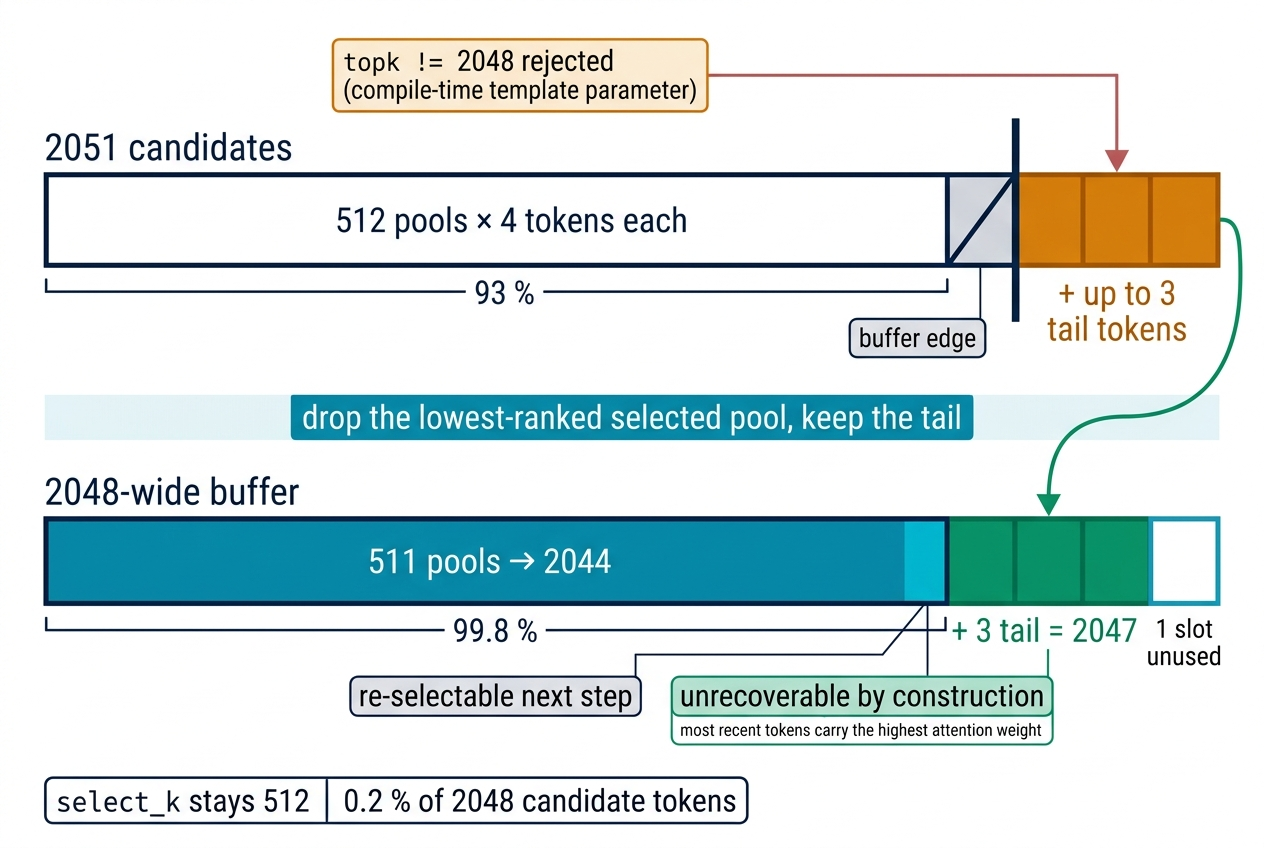
\includegraphics[width=\textwidth]{figures/ch14-candidate-squeeze.png}
\caption{Fix 2 of the NoPE overlay. The sparse indexer emits up to 2051
candidates --- 512 pools of 4 tokens, plus up to 3 tail tokens that have not
yet closed a pool --- while the SM120 prefill kernel's top-$k$ width is a
compile-time template parameter fixed at 2048. Dropping the lowest-ranked
pool costs 4 candidate tokens (0.2\,\%) that the indexer itself scored least
relevant and that a later step could in principle re-select; truncating the recent tail
instead would discard the highest-weighted tokens in a causal model, and no
pool expansion could ever recover them.}
\label{fig:qbet-squeeze}
\end{figure}

\section{A quantization backend from scratch}
\label{sec:qbet-exl3py}

With the KV geometry solved, the weights still need kernels. A quantization
backend in vLLM is best read as a claim of ownership: the registered module
takes responsibility for how the layers it claims are stored, sharded, and
multiplied, and every layer it does not claim falls through to the engine's
stock paths.
\repofile{overlay/exl3.py} (1{,}623 lines) is a complete vLLM quantization
backend --- not a patch of an existing one, but a new module registered with
\code{@register_quantization_config("exl3")} and dropped into the image's
quantization package (an 11-line companion patch adds \code{"exl3"} to
\code{ModelConfig}'s override list so vLLM will claim the checkpoint).
Its scope is deliberately narrow: \code{quant_method=exl3, codebook=mcg,
scope=glm53_routed_experts_only}. Only the routed experts run quantized;
everything else takes vLLM's stock \code{UnquantizedLinearMethod}.

Three design decisions define the file, and each is best read from the
failure it prevents. First, a packed-ABI disagreement between the checkpoint
and the kernels would be silent corruption --- so \textbf{the checkpoint ABI
is asserted, not assumed}. Each expert matrix ships as \code{trellis}
(packed int16 codes), \code{suh}/\code{svh} (fp16 input/output Hadamard
sign-scale vectors), and an int32 \code{mcg} marker whose value must be the
MCG multiplier \code{0xCBAC1FED};\footnote{Stored, in int32's signed
rendering, as $-877912083$.} \code{process_weights_after_loading} checks
that marker on \emph{every expert} and raises a hard \code{RuntimeError} on
mismatch --- corruption, never a warning. The exllamav3 dependency is pinned
to the same standard --- commit \code{c5d9c657}, version 0.0.43, the pin that
exposes the fused \code{exl3_moe} entry points.

Second, without the method actually claiming the layers, vLLM's default
loader would quietly expand every routed expert to BF16 --- tripling the
routed-expert footprint and OOMing the machine --- so \textbf{experts never
materialize in BF16}. \code{create_weights} registers only the packed
parameters --- the trellis tensors, Hadamard vectors, and markers for the
gate/up and down projections --- and then \emph{raises} if the dense buffers
\code{w13_weight} or \code{w2_weight} exist on the layer. That negative
promise, not the \code{"exl3"} registration itself, is what makes 164\,GiB
fit on two unified-memory GB10 nodes. TP=2 sharding follows the usual MoE
convention (gate/up column-wise, down row-wise, one all-reduce per layer),
with \code{_narrow_tp} raising on any non-divisible dimension.

Third, executing \code{exllamav3/__init__.py} would drag FlashAttention and
serving extras absent from this image into the boot --- so \textbf{the
dependency is imported surgically}. The backend needs exactly one class,
\code{LinearEXL3}, and \code{_install_exllamav3_namespace()} fabricates just
enough stub modules for
\code{exllamav3.modules.quant.exl3.LinearEXL3} to import cleanly through a
skeleton of its own package.\footnote{Stub \code{types.ModuleType} entries
for \code{exllamav3}, \code{exllamav3.modules}, and \code{exllamav3.model},
plus a fake \code{Config} class, leaving \code{.ext}, \code{.util}, and
\code{.modules.quant} real.} It is the same patch-discipline instinct as
\Cref{ch:patches}, applied to Python's import system: take exactly what you
need, and make every assumption about the rest explicit.

At runtime the fused path (\envvar{EXL3_FUSED_MOE=1}, the default) builds
GPU pointer tables for all nine tensor families (gate/up/down $\times$
trellis/suh/svh) and serves each decode layer with a single
\code{exllamav3_ext.exl3_moe} launch. The shared temp buffers are sized to
\envvar{EXL3_TEMP_ROWS_FUSED} rows per expert --- default 128. That number
is a measured boundary, not a guess: it defines who counts as a ``fat''
expert, and the next section is about what happens to them.

\section{The fat-expert tier ladder}
\label{sec:qbet-tiers}

Decode batches are small; the fused kernel's 128-row-per-expert budget covers
them in one graph-safe launch. Prefill is the opposite regime: at chunk size
2048, top-8 routing over 288 experts means essentially \emph{every} expert
activates, and the hottest experts see far more than 128 rows. (The P0
profile in \Cref{sec:qbet-warstory} measured 98.6\,\% of MoE layers hitting
the fat path at $\approx$920 rows for the hottest expert.) The fused kernel
simply skips any expert whose token count exceeds the temp rows, so fat
experts need a second pass --- and the backend offers four implementations of
that pass, arranged as a strict ladder resolved once, at weight load:

\begin{description}
  \item[kernel (E2)] direct trellis GEMMs --- \code{ext.exl3_fat_gemm} for
    the stacked gate+up projection and \code{ext.exl3_fat_gemm_scatter} for
    the down projection with fused routing (\Cref{sec:qbet-e2}).
  \item[batched (E1)] persistent scratch buffers; routing counts staged
    device-to-host on a side CUDA stream while the thin-expert launch
    proceeds; gate and up trellises stacked into one GEMM behind a single
    input Hadamard --- legal only because the checkpoint shares its input
    sign-scale vector (SUH) between gate and up, a fact \emph{verified at
    load} by \code{torch.equal} on the two halves of \code{w13_suh}.
    Without the E2 kernel this tier reconstructs fp16 weights into scratch
    and runs \code{ext.hgemm} plus an output-Hadamard pass.
  \item[sorted] reuses the already-sorted token/weight buffers so one
    \code{counts.tolist()} replaces all per-expert host syncs; contiguous
    slices are views.
  \item[legacy] the original Python loop over fat experts: per-expert
    \code{unique().tolist()}, \code{nonzero()}, three \code{LinearEXL3}
    forwards, SwiGLU, \code{index_add_} scatter --- many host syncs per
    layer.
\end{description}

Each tier's env knob implies the ones below it
(\envvar{EXL3_FAT_KERNEL=1}, the shipped default, implies batched and
sorted). The resolution logic is where the repository's failure philosophy
crystallizes:

\begin{lstlisting}[language=Python]
# resolve_exl3_fat_tier -- runs once, at weight load
if EXL3_FAT_KERNEL:
    if not (sym_exl3_fat_gemm and sym_exl3_fat_gemm_scatter):
        raise RuntimeError(...)   # "unset EXL3_FAT_KERNEL or serve an E2 image"
    if not shared_suh:
        tier, reason = "sorted", "shared_suh_absent"   # recorded, legitimate
    else:
        tier = "kernel"
elif EXL3_FAT_BATCHED: ...        # same shared-SUH gate
elif EXL3_FAT_SORTED:  tier = "sorted"
else:                  tier = "legacy"
\end{lstlisting}

Two outcomes that look superficially similar are treated in opposite ways.
An image whose extension lacks the E2 symbols while
\envvar{EXL3_FAT_KERNEL=1} is a \emph{configuration lie} --- the operator
asked for a kernel that does not exist. The backend fails closed at boot
with a \code{RuntimeError} naming the missing symbol, before the server can
take a request. A checkpoint that does not share SUH between gate and up
is merely a \emph{different checkpoint}: the stacked-GEMM optimization is
unavailable, so the tier degrades to \code{sorted} with the recorded reason
\code{shared_suh_absent} --- slower, correct, and visible in the diagnostics.

\begin{hblesson}
Degradation is legitimate; mismatch is fatal. A system may run slower than
configured when the \emph{data} does not support an optimization, provided
it records why --- but it must never run at all when the \emph{deployment}
contradicts its configuration. The boundary is who is wrong: if the
checkpoint lacks a property, the ladder steps down and says so; if the image
lacks a symbol the operator explicitly enabled, silently stepping down would
convert a build mistake into weeks of unexplained slow prefill. The GLM
recipe repository learned this concretely: before the recipe-stamp rebuild
mechanism landed in PR \ghissue{77}, \envvar{EXL3_FAT_KERNEL=1} on the older
public GHCR image had been a silent no-op --- exactly the failure mode the
load-time \code{RuntimeError} now makes impossible.
\end{hblesson}

\begin{figure}[htbp]
\centering
\begin{tikzpicture}[node distance=5mm and 12mm]
  \node[hbtitle] (t) {Fat-expert tier ladder --- resolved once at weight load};
  \node[hbgpu, below=4mm of t, minimum width=58mm] (k)
    {\textbf{kernel (E2)} --- direct trellis GEMMs\\exl3\_fat\_gemm + \_scatter};
  \node[hbbox, below=of k, minimum width=58mm] (b)
    {\textbf{batched (E1)} --- persistent scratch,\\stacked gate+up, side-stream D2H counts};
  \node[hbnode, below=of b, minimum width=58mm] (s)
    {\textbf{sorted} --- one counts.tolist(),\\contiguous slice views};
  \node[hbfaint, below=of s, minimum width=58mm] (l)
    {\textbf{legacy} --- python loop,\\per-expert host syncs};
  \draw[hbarrow] (k) -- (b);
  \draw[hbarrow] (b) -- (s);
  \draw[hbarrow] (s) -- (l);
  % gates
  \node[hbwarn, right=of k, minimum width=44mm] (boom)
    {EXL3\_FAT\_KERNEL=1,\\symbols missing:\\\textbf{RuntimeError at load}};
  \draw[hbfail] (k.east) -- (boom.west);
  \node[hbpatch, right=of b, minimum width=44mm] (suh)
    {shared gate/up SUH absent:\\degrade to \emph{sorted},\\reason recorded};
  \draw[hbarrow] (suh.west) -- (b.east);
  \draw[hbarrow] (suh.south) to[out=-90,in=0] (s.east);
  \node[hblabel, below=2mm of l, align=center]
    {each knob implies the tiers below it; shipped default EXL3\_FAT\_KERNEL=1};
\end{tikzpicture}
\caption{The fat-expert tier ladder in \code{overlay/exl3.py}. The highest
enabled tier wins, resolved at weight load. A missing kernel symbol under
\code{EXL3_FAT_KERNEL=1} is a deployment mismatch and fails the boot; a
checkpoint without shared SUH is a legitimate degradation to the sorted tier
with a recorded reason.}
\label{fig:qbet-ladder}
\end{figure}

\section{The road to PR~77}
\label{sec:qbet-warstory}

The top rung of that ladder --- the E2 kernel --- did not begin as a kernel
project. It began as a profiling assignment --- and two published failures.

\begin{hbwarstory}
The prefill investigation (\repofile{docs/improve-prefill.md}, 2026-08-29)
opened with a roofline that pointed at weight streaming: at MNBT 1024,
routed-expert traffic alone was estimated at $\ge$330\,ms of a
1.05--1.10\,s engine step, memory-bound at that chunk size. The plan's step
P0 was ``profile first --- decides everything,'' and it did: the torch
profiler attributed \textbf{63\,\%} of the 1.08\,s step (623\,ms) to
\code{moe_forward_shared}, but split it damningly. The fused
\code{exl3_moe} kernel itself was only 134\,ms; 64\,ms went to
\code{LinearEXL3} weight reconstruction and 52\,ms to the
\code{index_add_} fat scatter. On the CPU side, a single
\code{.nonzero().tolist()} host sync in the fat fallback burned
\textbf{29\,\% of CPU} (1.45\,s in a 3-step capture). The suspects the
roofline could not rank turned out to be innocent: KDA measured only
$\approx$6\,\% and the sparse indexer $\approx$4\,\%, both flat from 16k to
100k context. The bottleneck was not the quantized GEMM --- it was
everything wrapped \emph{around} it for fat experts.

The two obvious fixes both failed, and the repository published the failures with
the same prominence as the wins. P2a (GPU 128-row tiling of fat experts):
$-61$\,\% at 8k, reverted, kept behind \envvar{EXL3_MOE_ROW_TILE=0} as an
escape hatch. P2b (raising \envvar{EXL3_TEMP_ROWS_FUSED} to 1024 so the
fused kernel swallowed fat experts in one launch): slower on \emph{every}
rung, worst $-24$\,\% at 100k --- the trellis kernel does not sustain large
per-expert M. What survived was the modest MNBT 2048 keep ($+16$\,\% at 8k)
and an honest sentence: the aspirational ceiling was not reached ``so larger
chunks could not drop the LinearEXL3 fat tax.'' Three days later PR
\ghissue{77} removed the fat tax properly --- with a kernel shaped by
exactly what P0 had measured: no reconstruction, no separate Hadamard pass,
no host-syncing scatter. The failed experiments were not wasted work; they
were the specification. The same plan also priced what was never built: its
P7 entry costed UMA KV stage-out/stage-in for evicted sessions at
$\sim$790\,MB $\approx$ 4\,ms against $\sim$105\,s of recompute --- ``the
cheapest prefill speedup in the list.'' It remains unbuilt: the
investigation stopped after P2, and P3--P8 were never started.
\end{hbwarstory}

The arc is Part~I's measurement discipline (\Cref{ch:measurement},
\Cref{ch:perf}) replayed in a new repository: profile before touching anything,
publish reverts next to keeps, and let the profile --- not the roofline ---
pick what gets built. \Cref{fig:qbet-p0} collects what P0 measured beside
what each measurement eventually bought.

\begin{figure}[htbp]
\centering
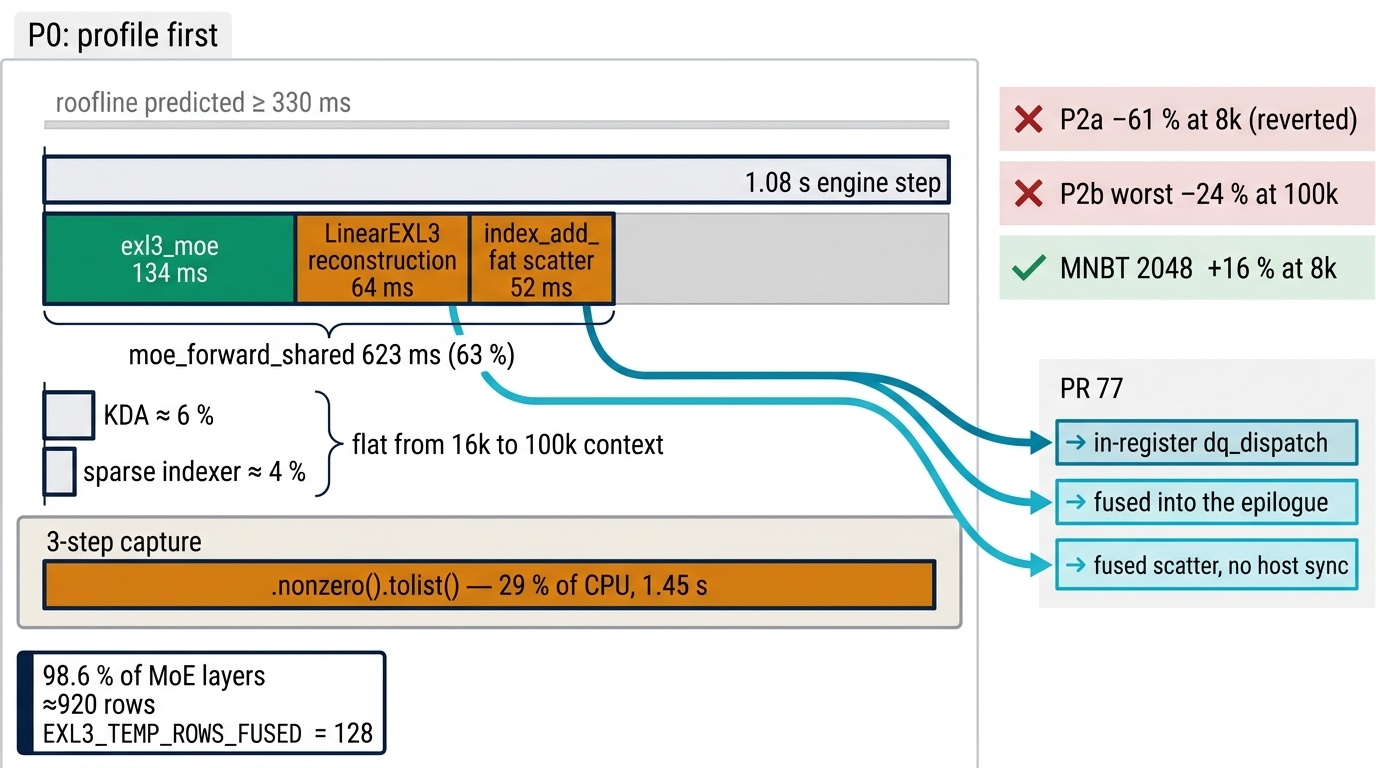
\includegraphics[width=\textwidth]{figures/ch14-p0-profile.png}
\caption{The P0 profile of 2026-08-29 and its consequences. The roofline
predicted a weight-streaming floor of at least 330\,ms; the measured
1.08\,s engine step put \code{moe_forward_shared} at 623\,ms (63\,\%),
inside which \code{exl3_moe} spent 134\,ms, \code{LinearEXL3} reconstruction
64\,ms, and the \code{index_add_} fat scatter 52\,ms, while KDA
($\approx$6\,\%) and the sparse indexer ($\approx$4\,\%) stayed flat from
16k to 100k context. A single \code{.nonzero().tolist()} host sync burned
29\,\% of CPU. Each measured cost maps to what PR~77 did with it; the two
reverted experiments are shown beside the keep.}
\label{fig:qbet-p0}
\end{figure}

\section{PR~77: the E2 kernels}
\label{sec:qbet-e2}

The kernel that specification produced is
\repofile{overlay/exl3_fat_gemm.cu} --- 295
lines of CUDA landed as PR \ghissue{77} in the GLM recipe repository's tracker
(2026-09-01, authored by community contributor plotarmordev). A 50-line
installer compiles it additively into \code{exllamav3_ext}, binding two
new entry points next to \code{exl3_moe}. It replaces the batched tier's
reconstruct-then-\code{hgemm}-then-Hadamard triple with GEMMs that consume
the trellis directly, and it is a compact tour of what a purpose-built
kernel buys over composed primitives: \Cref{fig:qbet-kernel} follows one weight through it.

\begin{itemize}
  \item \textbf{In-register dequantization.} \code{dq_dispatch<4, 1>}
    decodes the K4 MCG trellis words into register fragments per warp ---
    the 4-bit weights are never materialized in memory at all, not even in
    shared memory.
  \item \textbf{Tensor-core MMAs.} The inner loop is \code{ldsm4} loads plus
    \code{ptx_mma_m16n8k16} tensor-core instructions, accumulating in fp32
    across a $128 \times 16 \times 128$ tile.
  \item \textbf{XOR-swizzled shared memory.} Activation tiles are staged
    with a row-derived XOR swizzle matched on the \code{ldsm4} side,
    eliminating shared-memory bank conflicts without padding.
  \item \textbf{The output Hadamard fused into the epilogue.}
    \code{fat_had_ff_128} applies the 128-point output Hadamard transform
    entirely in the epilogue: an in-register 4-point butterfly, two 32-point
    stages built from warp shuffles (\code{shuffle_had_f2x32}), the
    $1/\sqrt{128}$ scale, then the fp16 \code{svh} sign-scales --- the
    separate output-Hadamard pass of the batched tier disappears into the
    GEMM's tail.
  \item \textbf{Scatter mode.} The down-projection entry point
    (\code{exl3_fat_gemm_scatter}) writes
    \code{out[token_idx[row] * N + n] += value * route_weight[row]},
    fusing the per-token route-weight multiply \emph{and} the token scatter
    into the kernel --- with a plain non-atomic \code{+=}. The race-freedom
    argument is a code comment worth quoting: ``One route per token reaches
    a given expert, and expert launches share this stream, so this
    accumulation is race-free.'' Within one expert each token appears once;
    across experts, launches serialize on the same CUDA stream. Correctness
    by scheduling invariant, not by atomics.
\end{itemize}

\begin{figure}[htbp]
\centering
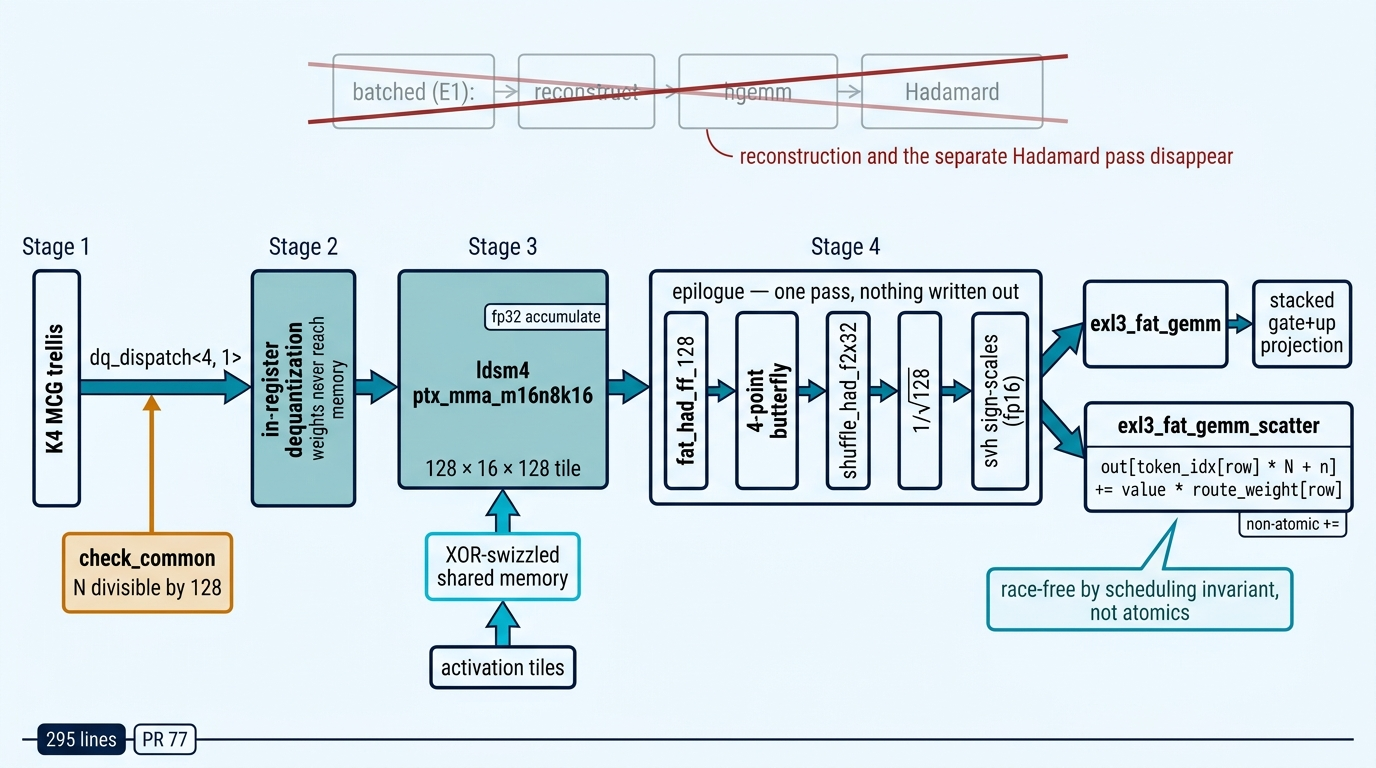
\includegraphics[width=\textwidth]{figures/ch14-e2-kernel-pipeline.png}
\caption{One pass through \repofile{overlay/exl3_fat_gemm.cu}. A K4 MCG
trellis word is decoded into register fragments by \code{dq_dispatch<4, 1>},
multiplied on tensor cores via \code{ldsm4} plus \code{ptx_mma_m16n8k16}
over a $128 \times 16 \times 128$ tile with fp32 accumulation, and finished
inside the epilogue --- Hadamard transform, sign-scales, route weight, and
in scatter mode the token scatter itself --- before any accumulator reaches
memory. The batched tier's reconstruct-then-\code{hgemm}-then-Hadamard
triple, shown struck through above, disappears entirely: the gain is not a
faster GEMM but the removal of the work between GEMMs.}
\label{fig:qbet-kernel}
\end{figure}

Read together the five are one pipeline rather than five separate tricks: a
weight leaves the trellis into registers, is multiplied on tensor cores, and
is finished --- transform, sign-scales, route weight, scatter --- before any
accumulator reaches memory. That is why the gain measured below is not a
faster GEMM but the disappearance of the work that used to happen between
GEMMs.

Guard rails are as characteristic as the fast path: \code{check_common}
rejects anything but K4 MCG tensors, wrong dtypes, non-contiguous inputs,
or an N not divisible by 128 --- the kernel refuses inputs it was not built
for rather than computing something plausible.

The measurement met the repository's own promotion bar: a controlled sequence (E2
on $\to$ legacy off $\to$ E2 on at MNBT 2048) with five unique-salt cold
samples per rung per boot, all 45 observations passing the cold gate with
complete separation. An independent second 2$\times$~DGX Spark kit
reproduced $+21.0$\,\% at 100K and $+20.4$\,\% at 300K.
\Cref{tab:qbet-e2} shows the pooled result that made E2 the production
prefill path (decode is unchanged --- decode batches never exceed the
128-row thin path).

\begin{table}[htbp]
\centering\small
\caption{PR~77 E2 fat-expert kernel: fully uncached prefill, MNBT 2048, five
unique-salt cold samples per rung per boot, 2026-09-01. Reproduced on an
independent second kit ($+21.0$\,\% at 100K, $+20.4$\,\% at 300K).}
\label{tab:qbet-e2}
\begin{tabular}{lrrr}
\toprule
Fully uncached rung & Legacy mean (\tokspersec{}) & PR~77 pooled mean (\tokspersec{}) & Gain \\
\midrule
$\approx$8K   & 941.04  & 1132.32 & $+20.33$\,\% \\
$\approx$100K & 1023.20 & 1241.71 & $+21.36$\,\% \\
$\approx$300K & 995.05  & 1201.02 & $+20.70$\,\% \\
\bottomrule
\end{tabular}
\end{table}

\section{The diagnostics contract}
\label{sec:qbet-diag}

A tier ladder resolved at load, degradations with recorded reasons, kernels
that may or may not be present in a given image --- none of it is auditable
without instrumentation. The E2 work shipped its instrumentation as a
versioned contract rather than ad-hoc logging. Its governing design
requirement is one most diagnostics surfaces never state: \emph{a stale
diagnostic that flatters the system is worse than no diagnostic}.

Two details enforce it. The counter reset
(\code{reset_exl3_fat_diag_counters()}) zeroes the runtime counters but
restarts the scratch-byte counters from the resident cache, so a windowed
read around exactly one cold request still reports honest byte counts
instead of pretending the persistent scratch is free. And the per-layer
labels (\code{_exl3_last_fat_fallback}, \code{_exl3_last_fat_reason},
\code{_exl3_last_apply}) are reset on \emph{every call}, so a
\code{"kernel"} label left over from an earlier prefill --- in the file's
words --- ``cannot masquerade through later decode/thin/row-tile calls.''

The surface those details protect is \code{_EXL3_FAT_DIAG}, a module-level
dict whose key set \emph{is} the API. \code{EXL3_FAT_DIAG_SCHEMA=1}
versions a fixed set of \textbf{32 keys}: load-time facts recording what
was resolved (configured versus effective tier and the degradation reason,
shared-SUH state, symbol availability, CUDA capability, TP rank), and
monotonic runtime counters recording what actually ran --- ``the ground
truth'' in the file's words. The stated rule is that the key set and the
schema number are extended only together, so an external monitor can parse
the output without scraping free-form text.

The whole snapshot renders as one greppable log line, emitted at load (as a
WARNING if the effective tier degraded from the configured one), again
whenever the resolved tier changes between layers, and every 42 layer-stat
records. The cadence is not arbitrary: GLM-5.3-Flash runs 42 routed-MoE
layers per engine step, so each line is exactly one step.
Chapter~\ref{ch:measurement}'s lesson that
instruments deserve regression tests reappears here as: instruments deserve
schemas.

\FloatBarrier

The 4-bit checkpoint stopped being a file on the Hub several sections ago.
What it actually is, on this kit, is a bundle of obligations: a pinned
mirror and a shard count that turn its bytes into an invariant, a KLD panel
that turns its quality into a number, an attention geometry the engine
cannot load until arithmetic reshapes the request, and a 1{,}623-line
backend plus 295 lines of CUDA that make its weights multipliable at all.
The vendor's paved path was never a convenience --- it is the accumulated
discharge of exactly those obligations, and stepping off it means signing
for them yourself, in code, with receipts.

\section*{Takeaways}

\begin{itemize}
  \item Part~II inverts Part~I's bet: the same 2$\times$~GB10 TP=2 kit, but
    a community 4-bpw EXL3 quant that must carry its own quality evidence,
    kernels, and supply chain --- and that supply chain is engineering, not
    a URL. A revision-pinned, byte-identical mirror and a 120-shard
    completeness gate make ``the weights are present'' a checked invariant.
  \item The KLD panel is the bet's receipt: 4\,bpw EXL3 at 0.024555 nats
    statistically ties official FP8's 0.024629 at 54\,\% of the bytes
    (176 vs.\ 328\,GB). The same panel, scoring NVFP4 at 0.060535, is why
    NVFP4 weights and \code{--moe-backend marlin} are banned outright.
  \item When the kernel zoo lacks your geometry, buy an existing kernel
    with memory: zero-padding the 512-dim NoPE latent into the 576-wide
    GLM\_NSA record is mathematically exact at $\approx$24\,\% more DSA KV,
    and the 2051-candidate squeeze discards the four candidates the indexer
    itself ranked least relevant rather than the causal tail no later pool
    expansion could recover.
  \item Degradation is legitimate, mismatch is fatal: a checkpoint that
    does not share gate/up SUH steps the fat-expert ladder down with a
    recorded reason; an image missing a symbol the operator explicitly
    enabled fails the boot instead of becoming a silent no-op.
  \item Profile before building: P0 overturned the roofline, two published
    reverts became PR \ghissue{77}'s specification, and the E2 kernels
    shipped a reproduced $+20$\,\% of uncached prefill behind a versioned
    32-key diagnostics schema.
\end{itemize}

\chaptertransition{Every byte this backend saves is still a byte the decode
step has to stream, and the only way to stop paying for a weight stream is
to stop taking the step --- which is precisely what the drafter riding on
top of this quant exists to do. DFlash2 is a separate $\approx$2.3\,GiB
model run at $k{=}7$, and it bills for itself in a seven-component
acceptance vector on every step: 0.98 sagging to 0.83 on structured output,
0.75 collapsing to 0.06 on prose --- two fingerprints so unalike they amount
to two serving machines inside one serve. There is a third shape, and when
bring-up produced it --- position~0 alive above six dead positions --- it
named a one-line cause that took no profiler, kernel trace, or bisection
to find.}

% =============================================================================
% Chapter 15 — A Second Drafter: DFlash2 and Acceptance Forensics
% =============================================================================
\chapter{A Second Drafter: DFlash2 and Acceptance Forensics}
\label{ch:dflash2}

During bring-up, one plausible-looking line of configuration --- pinning
\code{attention_backend=TRITON_ATTN} for the drafter --- dropped structured
decode from its 65.1 \tokspersec{} median to $\approx$29 and the accept ratio
from 0.959 to 0.31. Finding the cause took no profiler, kernel trace, or bisection.
Seven numbers found it: the per-position acceptance vector showed position~0
healthy while positions 1--6 lay dead, and that shape has exactly one
explanation. How a drafter comes to emit such a fingerprint, and how to read
it, is this chapter's subject.

The drafter in question is the GLM recipe's structurally different bet on
speculative decoding. \Cref{ch:specdecode} taught the subject through
DSpark: a block drafter baked into the DeepSeek checkpoint, drafting a
trained $\gamma{=}5$ block through a rank-256 Markov head, run at $k{=}6$
and later unlocked back to its trained $k{=}5$. DFlash2 is a \emph{separate}
$\approx$2.3\,GiB Qwen3-architecture draft model
(\code{incoai/GLM-5.3-Flash-DFlash2}), run at $k{=}7$ with a trained block
of 8. It wraps every draft layer in grouped dynamic convolutions and picks
its draft tokens by walking a lattice of candidate transitions in a single
Triton kernel. The economics are the same --- on a bandwidth-bound GB10,
every accepted draft token is a token that did not pay for a weight stream
--- but almost every implementation decision lands on the opposite side of
the design space from \Cref{ch:specdecode}, and so do the failure modes.

The chapter's second subject follows from the first: \emph{per-position
acceptance forensics}, a diagnostic method Part~I gestured at but never
needed as a primary instrument. With $k{=}7$, every decode step emits a
seven-component acceptance vector, and this recipe learned to read that
vector's \emph{shape} the way a cardiologist reads an ECG --- a gentle decay
means one thing, a front-loaded collapse another, and a healthy position~0
above six dead positions means something very specific indeed. The
TRITON\_ATTN incident in \Cref{sec:dflash2-triton} is the payoff: a
2$\times$ throughput regression diagnosed to a one-line attention-backend
cause purely from the fingerprint --- a localizing instrument cheaper than
any profiler.

\section{Two drafters, two philosophies}
\label{sec:dflash2-contrast}

It is worth fixing the contrast before descending into mechanism, because
the two recipes' war stories are mirror images. DSpark hides its cross-step
state in private ring buffers \emph{outside} vLLM's paged KV --- which is why
its saga (the ``Keys'' patches of \Cref{ch:specdecode}) was about a
condensing scheduler corrupting state the allocator could not see. DFlash2's
five sliding-window attention layers register \emph{real} KV specs
\emph{inside} the paged pool --- so its saga
(\Cref{sec:dflash2-slotshare}) was the opposite fight: convincing a hybrid KV
allocator, purpose-built for the target model's exotic geometry, to house a
guest without wrecking either party's accounting.

The drafting mechanisms differ just as sharply. DSpark predicts a whole
block from one anchor-plus-noise-queries pass and then biases each position's
logits with a low-rank Markov term conditioned on the previous pick. DFlash2
runs a genuine small transformer over the draft block, computes top-$k$
\emph{candidate sets} per position, scores every candidate-to-candidate
transition, and decodes a single best path through that lattice. And where
DSpark's operating point was argued back from $k{=}6$ to the trained
$k{=}5$, DFlash2 ships at its trained shape from day one: $k{=}7$, block~8,
draft tensor parallelism 2 (the \envvar{DFLASH_DRAFT_TP=2} default kept by
GLM repository PR \ghissue{48} after an A/B held both idle prefill and decode).
The serve wires it up with one JSON blob:

\begin{lstlisting}[language=jsonhb]
{"method":"dflash","model":"<DFLASH_MODEL_DIR>","num_speculative_tokens":7,
 "kv_cache_dtype":"auto","draft_sample_method":"probabilistic",
 "rejection_sample_method":"standard","draft_tensor_parallel_size":2}
\end{lstlisting}

The \code{kv_cache_dtype: auto} is load-bearing: the target's KV is the
packed \code{fp8_ds_mla} record, an MLA-only layout that dense draft
attention cannot consume, and SM121 has no FlashAttention-3/4 for plain FP8
KV. The installer's dtype guard therefore forces the draft cache to bf16
whenever the target cache is any FP8 or NVFP4 variant.

\section{Anatomy of DFlash2}
\label{sec:dflash2-anatomy}

What follows is a legend, not an inventory: position~0 of the acceptance
vector depends only on the anchor token, while positions 1--6 depend on the
block's taps, mask, and edge scores. Every part named here will be a
suspect in \Cref{sec:dflash2-triton}.

The stack is four overlay files: the drafter model
(\repofile{overlay/qwen3_dflash2.py}, 298 lines), the speculator walk
(\repofile{overlay/dflash2_speculator.py}, 250 lines), the installer
(\repofile{overlay/patch_dflash2.py}, 189 lines), and the KV-layout patch
(\repofile{overlay/patch_glm5_drafter_group.py}, 826 lines --- the subject of
\Cref{sec:dflash2-slotshare}). The model file is a port of upstream vLLM's
DFlash2 onto this older pinned image; its one divergence is candidate
top-$k$ extraction, done with a plain \code{torch.topk} over gathered logits
because the image's \code{LogitsProcessor} lacks \code{get_top_k_tokens}.

\subsection{Grouped dynamic convolutions with position-gated taps}

DFlash2 adds three things over the first-generation DFlash Qwen3 drafter.
The first is \code{DFlashGroupedConv}: a per-layer grouped dynamic
convolution that \emph{brackets} both attention and the MLP. Hidden states
split into \code{num_groups = hidden/group_size} groups; a
\code{kernel_projection} emits per-token deltas that are added to a static
\code{base_kernel} --- one coefficient set per side (the exact projection
shapes are in \Cref{fig:dflash2-anatomy}'s caption). Each decoder layer calls \code{prepare()} (conv
side 0, which also returns the side-1 coefficients) before attention and
\code{finish()} (side 1) after the MLP: a matched pre/post filter pair
around the whole layer.

The convolution itself is causal and depthwise over the last
\code{taps} positions, but --- and this is the detail everything in
\Cref{sec:dflash2-fingerprints} depends on --- it is \emph{restricted to the
draft block}. Positions are reduced modulo \code{block_size} (a bitwise AND
when the block is a power of two), and tap $t$ contributes only where the
in-block position is at least $t$. Nothing convolves across a draft-block
boundary; a token at in-block position 1 sees exactly one predecessor, no
matter how long the sequence is. With \code{block_size} defined as one plus
\code{num_speculative_tokens} --- $1 + k = 8$ for $k{=}7$, the bonus token
plus seven mask tokens --- the drafter's entire receptive structure is
engineered around that 8-slot frame.

\subsection{The candidate selector and the lattice walk}

The lattice is the abstraction to hold for the next few pages: the $k$ draft
positions form a graph whose nodes are each position's top-$k$ candidate
tokens and whose edges carry a score for one candidate following another, and
drafting is the choice of a single route through it rather than $k$
independent picks.

The second addition is \code{CandidateSelector}, a low-rank token-transition
scorer: a \code{predecessor_codebook} and \code{successor_codebook}, both
$[\mathrm{vocab}, \mathrm{rank}]$, plus a \code{hidden_projection} from
hidden size down to the rank. For each draft step $l$ it builds a full
$\mathrm{top}k \times \mathrm{top}k$ matrix of edge scores: the unary
logit of candidate $c$ at step $l$, plus an einsum coupling predecessors at
step $l{-}1$ to successors at step $l$, modulated by the projected hidden
state. The request's last accepted token (the anchor) seeds step~0.
The selector is wrapped in \code{set_model_tag("dflash2_candidate_selector")}
so \code{torch.compile} caches it separately from the draft head.

Decoding that lattice is the job of \code{_selector_walk_kernel} in
\repofile{overlay/dflash2_speculator.py}: a Triton kernel with one program
per request that walks the candidate lattice step by step. At each of the
$k$ steps it loads the top-$k$ scores conditioned on the previously chosen
candidate index, applies Gumbel-max sampling (probabilistic only when draft
logits are needed for rejection sampling; plain argmax at temperature~0),
records the chosen token and its realized score, and carries the chosen
index into the next step. The result is a Viterbi-style single-path decode
through the $k \times k$ edge scores. A companion
\code{_cache_draft_logits_kernel} maintains a sparse draft-logits cache for
the rejection sampler, erasing the previous step's cached candidate entries
to $-\infty$ and writing the new top-$k$ scores at the candidate token
positions. These are tiny kernels, and their compile shapes are exactly
what \Cref{sec:dflash2-warmup} exists to pre-warm.

\begin{figure}[htbp]
\centering
\adjustbox{max width=\textwidth}{%
\begin{tikzpicture}[node distance=6mm and 3mm]
  % ---- Row 1: the draft block with position-gated taps ----
  \node[hbtitle] (t1) {1.\ The 8-slot draft block: conv taps gated by in-block position};
  \node[hbfaint, below=4mm of t1.south west, anchor=north west, minimum width=17mm]
    (prev) {prev.\ block\\pos 7};
  \node[hbbox, right=5mm of prev, minimum width=13mm] (p0) {pos 0\\anchor};
  \node[hbnode, right=2.5mm of p0, minimum width=11mm] (p1) {pos 1};
  \node[hbnode, right=2.5mm of p1, minimum width=11mm] (p2) {pos 2};
  \node[hbnode, right=2.5mm of p2, minimum width=11mm] (p3) {pos 3};
  \node[hbfaint, right=2.5mm of p3, minimum width=20mm] (prest) {pos 4 \dots{} 7};
  \draw[dashed, thick, color=hbAccent]
    ($(prev.north east)!0.5!(p0.north west)+(0,2mm)$) --
    ($(prev.south east)!0.5!(p0.south west)+(0,-8mm)$);
  \node[hblabel, below=1mm of prev.south] {block boundary};
  \draw[hbfail] (prev.south) to[out=-60,in=-120] node[hblabel, below=0.5mm] {no tap crosses} (p0.south);
  \draw[hbok] (p0.south) to[out=-50,in=-130] (p1.south);
  \draw[hbok] (p0.south) to[out=-60,in=-120] (p2.south);
  \draw[hbok] (p1.south) to[out=-50,in=-130] (p2.south);
  \draw[hbok] (p2.south) to[out=-50,in=-130] (p3.south);
  \node[hblabel, right=2mm of prest.east, align=left]
    {tap $t$ active only\\where pos $\geq t$};
  % ---- Row 2: layer pipeline ----
  \node[hbtitle, below=17mm of prev.south west, anchor=north west] (t2)
    {2.\ Each decoder layer: dynamic conv brackets attention and MLP};
  \node[hbpatch, below=4mm of t2.south west, anchor=north west, minimum width=25mm]
    (kp) {kernel\_projection\\base + per-token $\Delta$};
  \node[hbbox, right=4mm of kp, minimum width=21mm] (c0) {grouped conv\\side 0 (prepare)};
  \node[hbnode, right=4mm of c0, minimum width=25mm] (attn) {attention\\non-causal in block};
  \node[hbnode, right=4mm of attn, minimum width=14mm] (mlp) {MLP};
  \node[hbbox, right=4mm of mlp, minimum width=21mm] (c1) {grouped conv\\side 1 (finish)};
  \draw[hbflow] (kp) -- (c0);
  \draw[hbflow] (c0) -- (attn);
  \draw[hbflow] (attn) -- (mlp);
  \draw[hbflow] (mlp) -- (c1);
  % ---- Row 3: selection ----
  \node[hbtitle, below=13mm of kp.south west, anchor=north west] (t3)
    {3.\ Path selection: one Triton program per request};
  \node[hbnode, below=4mm of t3.south west, anchor=north west, minimum width=27mm]
    (topk) {top-$k$ candidates\\+ unary logits};
  \node[hbnode, right=4mm of topk, minimum width=32mm]
    (edges) {edge scores $k \times k$\\pred./succ.\ codebooks};
  \node[hbgpu, right=4mm of edges, minimum width=30mm]
    (walk) {selector walk kernel\\Gumbel-max path};
  \node[hbgpu, right=4mm of walk, minimum width=22mm]
    (out) {drafts\\$d_1 \dots d_7$};
  \draw[hbflow] (topk) -- (edges);
  \draw[hbflow] (edges) -- (walk);
  \draw[hbflow] (walk) -- (out);
\end{tikzpicture}}
\caption{DFlash2 anatomy. Top: the 8-position draft block; grouped dynamic
convolution taps are gated so tap $t$ fires only at in-block positions
$\geq t$, and no tap ever crosses a block boundary. Middle: each decoder
layer wraps attention and MLP in a matched conv pre/post pair whose kernels
are the static base plus per-token projected deltas ---
\code{kernel_projection} is a \code{ReplicatedLinear} producing
$2 \times \mathrm{taps} \times \mathrm{num\_groups}$ coefficients over a
\code{base_kernel} of shape $[2, \mathrm{taps}, \mathrm{hidden}]$. Bottom:
per step, a low-rank predecessor/successor codebook scores every candidate
transition, and a one-program-per-request Triton kernel decodes a single
Viterbi-style path through the lattice; \code{BLOCK_K} is the next power of
two at or above \code{selector_top_k}, at \code{num_warps=1}, and because the
image's \code{gumbel.py} predates \code{gumbel_noised_argmax} the walk
vendors it as a \code{@triton.jit} helper --- temperature-scaled logits
plus $-\log(-\log u)$ noise, with \code{log1p} in fp32 for precision.}
\label{fig:dflash2-anatomy}
\end{figure}

\subsection{Non-causal by declaration, and the installer}

The third piece is a config bit with an outsized blast radius: the incoai
checkpoint ships \code{is_causal: false}. Draft attention is
\emph{bidirectional inside the draft block} --- the mask must let every draft
position attend to every other position in its block. The installer,
\repofile{overlay/patch_dflash2.py}, is the overlay's standard fail-closed
file-copier: it copies the two modules into the vLLM tree, registers
\code{DFlash2DraftModel} in the speculative-model registry, teaches the
DFlash1 base model to honor checkpoint \code{is_causal} ahead of its
SWA-implies-causal heuristic (so a DFlash2 checkpoint ``does not silently
draft as causal DFlash1,'' as the image self-check
\repofile{tests/test_exl3_overlay.py} pins in so many words). It also
installs the draft-KV dtype guard, dispatches \code{method == "dflash"} to
\code{DFlash2Speculator} when the DFlash2 architecture is present, and
\code{compile()}-checks all five touched files before finishing. On SM121
the backend selector already prefers FLASH\_ATTN for non-causal dense
sliding-window attention, so the recipe deliberately leaves the draft
attention backend \emph{unset}. What happens when an operator pins it anyway
is \Cref{sec:dflash2-triton}.

\section{The measured envelope}
\label{sec:dflash2-envelope}

Mechanism in hand, the next question is what the machine actually delivers.
Two instruments define the performance record. The official sparkDash decode
bench (2026-08-28: DFlash2 $k{=}7$, temperature 0, thinking off, 400 tokens,
CUDA graphs, fused EXL3 MoE, structured and code prompts) gives the
concurrency envelope in \Cref{tab:dflash2-envelope}; the lab's own
\repofile{tests/bench_decode.py} (median of 5 runs $\times$ 400 tokens,
2026-08-30, the C4 keep, \envvar{DFLASH_DRAFT_TP=2}) gives the
per-domain split that the rest of this chapter turns into a diagnostic
method.

\begin{table}[htbp]
\centering\small
\caption{Decode envelope, official sparkDash bench (DFlash2 $k{=}7$,
temperature 0, thinking off, 400 tokens, 2026-08-28). Stream \tokspersec{}
is per request; aggregate sums all streams.}
\label{tab:dflash2-envelope}
\begin{tabular}{lrrr}
\toprule
Concurrency & TTFT & Stream \tokspersec{} & Aggregate \tokspersec{} \\
\midrule
$\times 1$ & 719\,ms & 62.9 & 62.9 \\
$\times 2$ & 6.62\,s & 51.7 & 103.3 \\
$\times 4$ & 6.30\,s & 37.1 & 146.5 \\
\bottomrule
\end{tabular}
\end{table}

The lab medians, all on the same protocol (median of five 400-token
generations, 2026-08-30, \envvar{DFLASH_DRAFT_TP}\code{=2}):
\textbf{structured} decode (counting 1 to 200) runs
65.1 \tokspersec{} at accept ratio 0.959 and \textbf{6.71 tokens per step};
\textbf{prose} (a hash-map explanation) runs 27.1 \tokspersec{} at accept
0.341 and 2.39 tokens per step. The prior \envvar{DFLASH_DRAFT_TP=1}
configuration measured 61.7\,/\,26.9 on the same phases --- sharding the
drafter across both ranks was a keep, not a wash, which is why GLM repository PRs
\ghissue{48} and \ghissue{49} baked it in.

Long-context and mixed sessions
($\approx$60--100k of KV in play) settle to 24--27 \tokspersec{}, and the
MTP $k{=}2$ rollback path (\code{SPEC_METHOD=mtp}) idles at
$\approx$24.6 \tokspersec{} --- the floor the DFlash2 bet is measured
against. The 2.4$\times$ structured-versus-prose spread inside a single
serve is the largest of any number in this table, and it is entirely an
acceptance story: the hardware, weights, and step cost are identical; only
the drafter's hit rate differs.

\section{Accept vectors as fingerprints}
\label{sec:dflash2-fingerprints}

\Cref{ch:specdecode} measured per-position acceptance and used it to choose
$k$. This recipe goes a step further: \repofile{tests/bench_decode.py}
records the full vector on every run --- position $i$'s rate is the counter
delta of \code{position="i"} accepts divided by the delta of draft rounds
--- and the lab reads the \emph{shape} as a first-class diagnostic. The two
production fingerprints (lab medians, 2026-08-30):

\begin{table}[htbp]
\centering\small
\caption{Per-position acceptance of the DFlash2 $k{=}7$ block
(\repofile{tests/bench_decode.py} lab medians, 2026-08-30,
\envvar{DFLASH_DRAFT_TP=2}).}
\label{tab:dflash2-vectors}
\begin{tabular}{l ccccccc r}
\toprule
Phase & pos 0 & pos 1 & pos 2 & pos 3 & pos 4 & pos 5 & pos 6 & \tokspersec{} \\
\midrule
Structured & 0.98 & 0.98 & 0.94 & 0.94 & 0.91 & 0.83 & 0.83 & 65.1 \\
Prose      & 0.75 & 0.58 & 0.41 & 0.28 & 0.16 & 0.09 & 0.06 & 27.1 \\
\bottomrule
\end{tabular}
\end{table}

\begin{figure}[htbp]
\centering
\begin{tikzpicture}[x=1cm,y=42mm]
  \foreach \y/\l in {0.2/0.2, 0.4/0.4, 0.6/0.6, 0.8/0.8, 1.0/1.0} {
    \draw[hbSteel!25] (0,\y) -- (12.6,\y);
    \node[hblabel, left=1mm] at (0,\y) {\l};
  }
  \draw[thick, hbSteel] (0,0) -- (12.6,0);
  \draw[thick, hbSteel] (0,0) -- (0,1.05);
  % structured (green) / prose (amber-warn) grouped bars, group pitch 1.7
  \foreach \p/\vs in {0/0.98, 1/0.98, 2/0.94, 3/0.94, 4/0.91, 5/0.83, 6/0.83} {
    \fill[hbGreen!60] ({0.55+\p*1.7},0) rectangle ({1.05+\p*1.7},\vs);
    \node[hblabel] at ({0.80+\p*1.7},{\vs+0.045}) {\vs};
  }
  \foreach \p/\vp in {0/0.75, 1/0.58, 2/0.41, 3/0.28, 4/0.16, 5/0.09, 6/0.06} {
    \fill[hbAmber!70] ({1.10+\p*1.7},0) rectangle ({1.60+\p*1.7},\vp);
    \node[hblabel] at ({1.35+\p*1.7},{\vp+0.045}) {\vp};
  }
  \foreach \p in {0,1,2,3,4,5,6} {
    \node[hblabel] at ({1.075+\p*1.7},-0.06) {pos \p};
  }
  \fill[hbGreen!60] (2.6,-0.19) rectangle (3.0,-0.13);
  \node[hblabel, anchor=west] at (3.1,-0.16) {structured (0.959 overall)};
  \fill[hbAmber!70] (7.0,-0.19) rectangle (7.4,-0.13);
  \node[hblabel, anchor=west] at (7.5,-0.16) {prose (0.341 overall)};
\end{tikzpicture}
\caption{The two production fingerprints of the DFlash2 $k{=}7$ block (lab
medians, 2026-08-30). Structured decode holds a flat, slowly sagging vector
--- 0.98 down to only 0.83 at position 6 --- yielding 6.71 accepted tokens
per step. Prose decays geometrically from 0.75 to 0.06: the drafter is
healthy, the \emph{domain} is unpredictable. A third shape --- position 0
healthy, positions 1--6 dead --- appears in
\Cref{sec:dflash2-triton} and means neither of these things.}
\label{fig:dflash2-fingerprints}
\end{figure}

Reading the shapes: the \emph{structured} vector is nearly flat. Once the
model is emitting ``\dots{} 57 58 59 \dots'' the continuation is close to
deterministic, so even position 6, conditioned on six earlier guesses all
being right, still lands 83\,\% of its drafts. That is what a
well-conditioned drafter looks like when the domain cooperates, and it is
why structured throughput (65.1 \tokspersec{}) approaches the ideal
$(k{+}1)$-fold amortization of the step cost.

The \emph{prose} vector is a
clean geometric decay: position 0 at 0.75 says the drafter's single-token
prediction is decent; the roughly-halving tail says errors compound ---
each position's acceptance is conditioned on the whole prefix before it
surviving rejection sampling. Nothing is broken; free text simply carries
more entropy than the drafter can absorb, and 2.39 tokens per step is what
that entropy costs --- the second of the four shapes keyed in
\Cref{fig:dflash2-accept-key}.

\begin{hblesson}
The overall accept ratio is one number and it aliases badly: prose at 0.341
and a genuinely broken drafter at 0.31 read as neighbors on a dashboard.
The per-position \emph{vector} disambiguates in one glance, because
different faults live at different positions. Uniform depression across all
positions: the drafter's inputs are wrong (bad aux features, wrong
checkpoint). Geometric decay from a healthy position 0: domain entropy ---
not a fault at all. Healthy position 0 with a dead tail: something is
severing the \emph{intra-block} machinery --- exactly the taps, masks, and
edge scores of \Cref{fig:dflash2-anatomy} --- because position 0 is the only
draft slot that does not depend on in-block context. Publish the vector with
every benchmark, not just the ratio; it is the difference between ``decode
is slow'' and a component-level diagnosis.
\end{hblesson}

\begin{figure}[htbp]
\centering
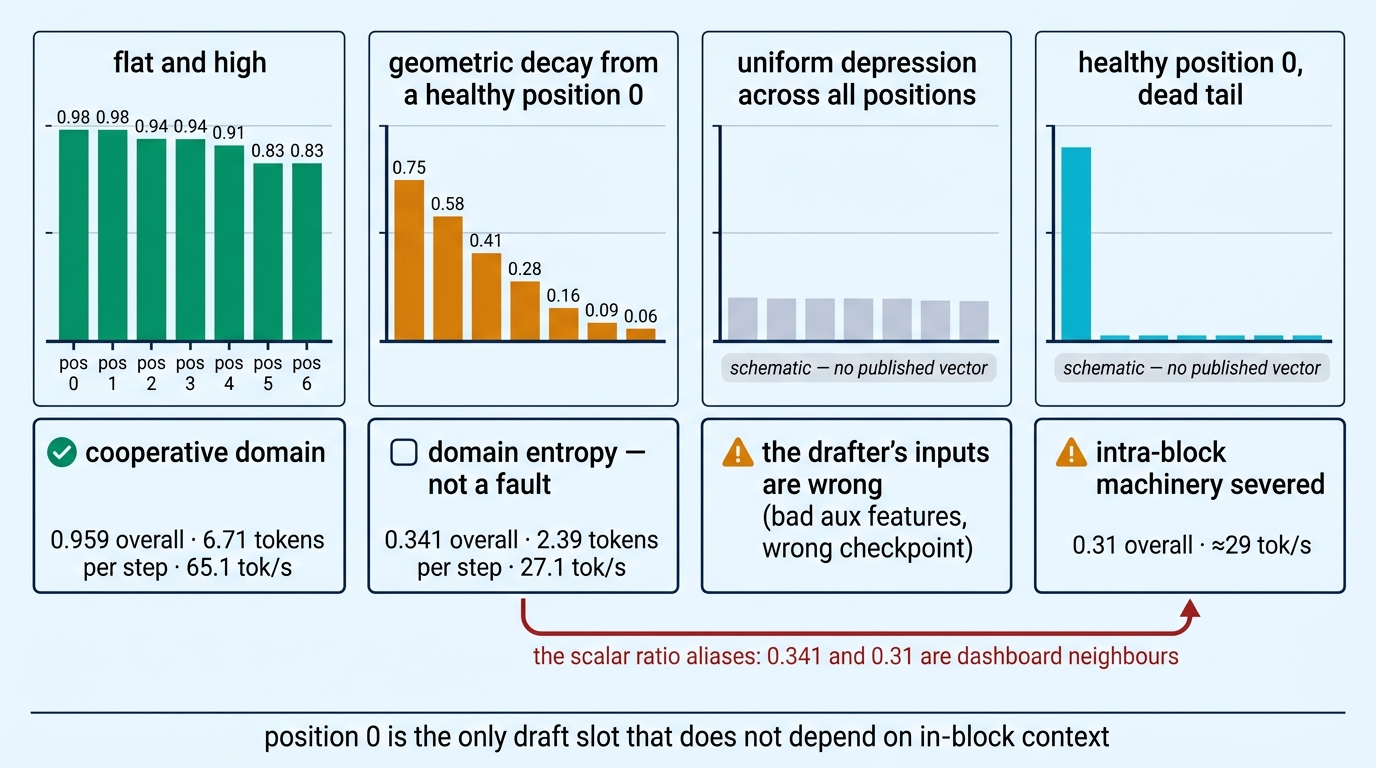
\includegraphics[width=\textwidth]{figures/ch15-accept-fingerprints.png}
\caption{The fingerprint key. With $k{=}7$ every decode step emits a
seven-component acceptance vector, and its shape names the fault. Flat and
high is a cooperative domain (structured decode, 0.959 overall, 6.71 tokens
per step). Geometric decay from a healthy position 0 is domain entropy rather
than a fault (prose, 0.341 overall, 2.39 tokens per step). Uniform depression
across all positions says the drafter's inputs are wrong. A healthy position 0
above a dead tail says the intra-block machinery --- taps, mask, or edge
scores --- has been severed, because position 0 is the only draft slot that
does not depend on in-block context; that is the shape
\Cref{sec:dflash2-triton} diagnoses at 0.31 overall and $\approx$29
\tokspersec{}. The first two panels are plotted from the 2026-08-30 lab
medians; the last two are schematic, since a broken run's per-position values
were not published. The overall ratio cannot tell panels 2 and 4 apart ---
0.341 and 0.31 are dashboard neighbours.}
\label{fig:dflash2-accept-key}
\end{figure}

\section{The TRITON\_ATTN collapse}
\label{sec:dflash2-triton}

The lab did not have to imagine that third shape; bring-up produced a
specimen.

\begin{hbwarstory}
During bring-up, pinning \code{attention_backend=TRITON_ATTN} in the
speculative config --- a plausible-looking act of determinism on a machine
where backend auto-selection had caused grief elsewhere --- dropped
structured decode from 65.1 to $\approx$29 \tokspersec{} and the accept
ratio from 0.959 to 0.31. The overall ratio alone would have suggested a
broken drafter: wrong weights, wrong taps, corrupted aux features. The
fingerprint said otherwise: \emph{position 0 stayed healthy while positions
1--6 collapsed}. Position 0 is drafted from the anchor alone; positions 1--6
require the block's bidirectional attention. A dead tail under a live head
means the drafter's forward pass is fine and its in-block visibility is not
--- the signature of a \emph{causal mask inside the draft block}. And that
is exactly what it was: on this image, TRITON\_ATTN's mask is causal inside
the draft block --- the SM120 image received a non-causal mask fix that this
SM121 image lacks. Every draft position could therefore attend only
backward, and DFlash2 degenerated into a crippled causal drafter. The fix is to not
pin the backend at all: SM121 auto-selects FLASH\_ATTN for non-causal dense
SWA. The README now carries the requirement four times --- as an explicit
warning in the drafter and bench sections, again in the knob table, and once
more on the ``Do not'' list --- a ban proportionate to how reasonable the
mistake looks.
\end{hbwarstory}

\begin{figure}[htbp]
\centering
\adjustbox{max width=\textwidth}{%
\begin{tikzpicture}[x=5.4mm,y=5.4mm,font=\scriptsize]
  % ---- left: non-causal mask (correct) --------------------------------
  \begin{scope}
    \node[hbtitle,anchor=south] at (4,8.9) {non-causal in block};
    \node[hblabel,anchor=south] at (4,8.3) {\code{is_causal: false}};
    \foreach \r in {0,...,7}{
      \foreach \c in {0,...,7}{
        \fill[hbGreen!45] (\c,7-\r) rectangle ++(1,1);
        \draw[hbSteel!50,line width=0.2pt] (\c,7-\r) rectangle ++(1,1);}}
    \foreach \i in {0,...,7}{
      \node[hblabel] at (\i+0.5,8.0) {\i};
      \node[hblabel] at (-0.45,7.5-\i) {\i};}
    \draw[teal,line width=0.9pt] (0,7) rectangle (8,8);
    \node[hblabel,anchor=north,align=center,text width=44mm] at (4,-0.25)
      {SM121 auto-selects FLASH\_ATTN\\for non-causal dense SWA};
  \end{scope}
  % ---- right: causal-in-block mask (the bug) --------------------------
  \begin{scope}[xshift=12.2cm]
    \node[hbtitle,anchor=south] at (4,8.9) {causal in block};
    \node[hblabel,anchor=south] at (4,8.3) {\code{attention_backend=TRITON_ATTN}};
    \foreach \r in {0,...,7}{
      \foreach \c in {0,...,7}{
        \ifnum\c>\r \fill[white] (\c,7-\r) rectangle ++(1,1);
          \draw[clueerror!55,line width=0.35pt] (\c,7-\r) -- ++(1,1);
        \else \fill[lightgray!45] (\c,7-\r) rectangle ++(1,1);\fi
        \draw[hbSteel!50,line width=0.2pt] (\c,7-\r) rectangle ++(1,1);}}
    \foreach \i in {0,...,7}{
      \node[hblabel] at (\i+0.5,8.0) {\i};
      \node[hblabel] at (-0.45,7.5-\i) {\i};}
    \draw[teal,line width=0.9pt] (0,7) rectangle (8,8);
    \draw[clueerror,line width=0.7pt] (-1.15,0) -- (-1.15,7);
    \node[hblabel,rotate=90,anchor=south,align=center,color=clueerror]
      at (-1.4,3.5) {positions 1--6 need\\bidirectional attention};
    \node[hblabel,anchor=north,align=center,text width=48mm] at (4,-0.25)
      {the SM120 image received a non-causal mask fix\\that this SM121 image lacks};
  \end{scope}
  % ---- shared annotations --------------------------------------------
  \node[hblabel,anchor=west,align=left,color=teal] at (8.6,7.5)
    {position 0 needs no\\in-block context};
  \node[hbnode,anchor=north west,align=left,font=\scriptsize] at (-1.6,12.8)
    {\code{block_size = 1 + k = 8}\\bonus token $+$ seven mask tokens};
  % ---- accept strip: seven draft positions ---------------------------
  \node[hblabel,anchor=east] at (-0.6,-4.1) {accepted};
  \foreach \p in {0,...,6}{
    \ifnum\p=0 \fill[hbGreen!55] (\p*1.5,-4.6) rectangle ++(1.2,1.0);
    \else \fill[clueerror!30] (\p*1.5,-4.6) rectangle ++(1.2,1.0);\fi
    \draw[hbSteel!60] (\p*1.5,-4.6) rectangle ++(1.2,1.0);
    \node[hblabel] at (\p*1.5+0.6,-5.0) {pos \p};}
  \node[hblabel,anchor=west,align=left] at (10.8,-4.1)
    {healthy head, dead tail --- the fingerprint\\that named the cause};
  \node[hbnode,anchor=north west,align=left,font=\scriptsize] at (0,-5.9)
    {$65.1 \rightarrow {\approx}29$ \tokspersec{} \quad
     $0.959 \rightarrow 0.31$};
  \node[hbbox,anchor=north west,font=\scriptsize] at (9.4,-5.9)
    {do not pin the backend};
\end{tikzpicture}}
\caption{What pinning \code{attention_backend=TRITON_ATTN} changed inside the
drafter's 8-slot block. Left: the non-causal mask the drafter is trained
for, where every one of the eight slots sees every other. Right: the causal
mask this SM121 image applies, in which slot $j$ can only see slots
$\leq j$. Row 0 is identical under both --- position 0 is drafted from the
anchor alone --- while positions 1--6 lose exactly the in-block visibility
they depend on. That is why the measured fingerprint showed a healthy head
and a dead tail, and why decode fell from 65.1 to $\approx$29
\tokspersec{} at 0.31 acceptance.}
\label{fig:dflash2-mask}
\end{figure}

The incident is the whole argument for acceptance forensics in miniature.
No profiler, no kernel trace, no bisection: one benchmark run with
per-position telemetry localized the fault to ``whatever provides positions
1--6 with visibility into the block,'' and the candidate list at that
address has exactly one entry. It also sharpens a Part~I lesson.
\Cref{ch:specdecode} warned that probes lie about acceptance ---
numbered-word prompts versus live prose. The GLM recipe internalizes that by
making \emph{both} fingerprints canonical: structured and prose are each
measured, each published with dates, and a regression is judged against the
matching fingerprint, never against the other one.

\section{Housing the drafter: padded slot-share}
\label{sec:dflash2-slotshare}

Reading the drafter's vectors is one half of operating it; the other half
is giving it somewhere to live. DSpark's drafter state lived outside the
allocator; DFlash2's lives inside
it, and getting it there took three failed boots. The target model's KV is
already the most baroque object in either repository: a hybrid pool of packed
\code{fp8_ds_mla} MLA layers, mamba groups, and an indexer tail, managed by
a GLM-5-Next fast path in vLLM's \repofile{v1/core/kv_cache_utils.py} that
recognizes exactly those species. The DFlash2 drafter registers five plain
\code{SlidingWindowSpec} layers --- a sixth species --- and the fast path's
response was to return \code{None}, dropping the whole model onto the
generic uniform-page path. That path provably cannot serve GLM-5.3-Flash:
page unification rescales the indexer tail's block away from its pool size,
and boot dies at warmup's shape assert. That is boot failures 6 and 7 of the
bring-up lane (\repofile{lane1_fail6.log}, \repofile{lane1_fail7.log} on
host ``Reddie'').

\begin{hbnote}
The interim workaround --- give the drafter standalone per-layer tensors ---
booted, but each of the five SWA layers inherited the MLA \emph{manager}
block, making every drafter page tens of MiB. Even compacted to its own
64-token blocks, the standalone drafter burned five independent sets of
BlockPool IDs: a single $\approx$36k-token session peaked at
\textbf{44.6\,\%} of the entire KV pool.
\end{hbnote}

The real fix, \repofile{overlay/patch_glm5_drafter_group.py}, is the
overlay's largest patch: fourteen anchored edits (each anchor must occur
exactly once; \code{ast.parse} after every mutation; marker
\code{DFLASH2-DRAFTER-GROUP}) that teach the fast path to append \emph{one}
extra KV group for the drafter --- last, so every existing group id stays
stable --- and to choose among three geometries:

\begin{itemize}
  \item \textbf{Padded slot-share} (deployed): the drafter keeps a compact
    manager block of \textbf{64} tokens but declares
    \code{page_size_padded} equal to the MLA page, and drafter layer $i$
    \emph{co-owns MLA tensor $i$} via \code{shared_by} at disjoint block ids
    drawn from the one shared BlockPool --- the same co-ownership trick the
    mamba layers already use. Per-block pool bytes are unchanged, so the
    drafter adds \textbf{zero bytes} to the pool; its sliding window bounds
    it to a handful of block ids per request. The scheduler's block-size
    LCM stays sane: $\mathrm{lcm}(3584, 64) = 3584$.
  \item \textbf{Exact fit} (rejected corner): rescale the drafter block so
    its page equals the MLA page exactly; on this model's geometry that
    only lands at MLA blocks of 16{,}384 tokens or more.
  \item \textbf{Standalone tensors} (rejected corner): the last resort,
    only if there were ever more drafter layers than MLA tensors.
\end{itemize}

The deployed mode is easier to hold as tenancy than as allocation: the
drafter is not given pages of its own but writes into block ids nobody else
is using, inside pages the MLA layers already own --- which is why its cost
is zero bytes rather than merely a small number of them.

\begin{figure}[htbp]
\centering
\adjustbox{max width=\textwidth}{%
\begin{tikzpicture}[node distance=5mm and 4mm]
  \node[hbtitle] (t) {Padded slot-share: drafter SWA pages inside the MLA pool};
  % drafter layers, left column
  \node[hbgpu, below=5mm of t.south west, anchor=north west, minimum width=24mm] (d0) {drafter SWA 0};
  \node[hbgpu, below=2.5mm of d0, minimum width=24mm] (d1) {drafter SWA 1};
  \node[hbfaint, below=2.5mm of d1, minimum width=24mm] (dd) {\dots};
  \node[hbgpu, below=2.5mm of dd, minimum width=24mm] (d4) {drafter SWA 4};
  % MLA tensors, right side: strips of blocks
  \node[hbbox, right=24mm of d0, minimum width=70mm, minimum height=9mm] (m0)
    {\makebox[52mm][l]{MLA tensor 0}};
  \node[hbbox, right=24mm of d1, minimum width=70mm, minimum height=9mm] (m1)
    {\makebox[52mm][l]{MLA tensor 1}};
  \node[hbfaint, right=24mm of dd, minimum width=70mm, minimum height=9mm] (md) {\dots};
  \node[hbbox, right=24mm of d4, minimum width=70mm, minimum height=9mm] (m4)
    {\makebox[52mm][l]{MLA tensor 4}};
  \node[hbfaint, below=2.5mm of m4, minimum width=70mm, minimum height=9mm] (m5)
    {MLA tensors 5--11 (MLA only, untouched)};
  % green sub-blocks inside m0/m1/m4 at the right edge
  \fill[hbGreen!45] ($(m0.east)+(-11mm,-3.2mm)$) rectangle ($(m0.east)+(-2mm,3.2mm)$);
  \node[hblabel, font=\tiny, anchor=east] at ($(m0.east)+(-12mm,1.2mm)$) {SWA ids};
  \fill[hbGreen!45] ($(m1.east)+(-11mm,-3.2mm)$) rectangle ($(m1.east)+(-2mm,3.2mm)$);
  \node[hblabel, font=\tiny, anchor=east] at ($(m1.east)+(-12mm,1.2mm)$) {SWA ids};
  \fill[hbGreen!45] ($(m4.east)+(-11mm,-3.2mm)$) rectangle ($(m4.east)+(-2mm,3.2mm)$);
  \node[hblabel, font=\tiny, anchor=east] at ($(m4.east)+(-12mm,1.2mm)$) {SWA ids};
  % shared_by arrows
  \draw[hbok] (d0.east) -- node[hblabel, above=0.2mm] {shared\_by} (m0.west);
  \draw[hbok] (d1.east) -- (m1.west);
  \draw[hbok] (d4.east) -- (m4.west);
  % pool group and annotations
  \begin{scope}[on background layer]
    \node[hbgroup, fit=(m0)(m5), label={[hblabel]below:{one shared BlockPool of
      fp8\_ds\_mla pages --- byte cost unchanged, drafter adds zero bytes}}] {};
  \end{scope}
  \node[hblabel, align=left, anchor=north west]
    at ($(d4.south west)+(0,-21mm)$)
    {manager block 64 $=$ kernel block\\page\_size\_padded $=$ MLA page\\window
     $\rightarrow$ $\approx$49 blocks/request/layer};
\end{tikzpicture}}
\caption{The deployed padded slot-share geometry of
\repofile{overlay/patch_glm5_drafter_group.py}. Each of the drafter's five
sliding-window layers co-owns one MLA tensor via \code{shared_by},
allocating its 64-token blocks at disjoint block ids from the same pool.
Because \code{page_size_padded} equals the MLA page and the manager block
equals the kernel block, per-block pool accounting is untouched: the drafter
costs zero additional bytes, and its window bounds it to roughly 49 blocks
per request per layer.}
\label{fig:dflash2-slotshare}
\end{figure}

One constraint in the deployed mode was bought with the lane's third failed
boot (\repofile{lane1_fail8.log}): \code{page_size_padded} is only safe when
the manager block \emph{equals} the kernel block. In the failing
configuration, FlashInfer chose a kernel block of 64 inside a 2{,}304-token
manager block; the strided view applied the full per-page stride per
\emph{kernel} block, and reads ran off the end of the tensor. The deployed
geometry pins both to 64 --- one kernel block per padded page --- and the
patch's validator rejects any padded layout where a backend would split the
block.

The patch also carries an upgrade ladder (v2 compact-64
$\rightarrow$ v3 padded slot-share $\rightarrow$ v4
allow-padded-in-layout) so that a GHCR image already patched at any
historical version converges to the current one instead of failing the
anchor match --- fail-closed patching, \Cref{ch:patches} style, extended
across its own history. A long ``runner-side audit'' docstring records why
no model-runner edits are needed at all.

The receipts: the $\approx$36k session that peaked at 44.6\,\% of KV under
standalone tensors dropped to $\approx$\textbf{16\,\%} under padded
slot-share; three concurrent $\approx$256k sessions --- the original failure
case --- now fit (peak 29.5\,\% with two in flight); and the default context
was raised to the full 1M. The 2026-08-29 padded slot-share boot logged a
\textbf{1{,}754{,}237-token} KV pool, and the boot line
\code{padded slot-share block=64 mla_page=2351104 (was block=16);
draft_bytes/token=2048} is the durable receipt.

\section{Warming the walk: the JIT shape ladder}
\label{sec:dflash2-warmup}

Housing settled the drafter's bytes; its kernels still start cold. A
drafter built out of small Triton kernels has a cold-start problem: every
distinct launch shape JIT-compiles on first use, and on a two-rank TP serve
a mid-serve compile stall on one rank can trip collective timeouts. The
recipe's answer, \repofile{scripts/boot-shape-warmup.sh}, runs after
\code{/health} and fires \emph{real API requests} so that every shape the
serving geometry can produce is compiled before the first client arrives.
Persistent Triton/TileLang cache mounts ride along, so each shape compiles
once per image, not once per container.

The two discoveries that follow are both about deriving a warmup from the
serving geometry rather than from habit: the set of launch shapes that can
actually occur turns out to be finite and computable, and the sampler quietly
adds a second dimension to it that no reasonable ladder would think to cover.

The first discovery: the ladder can be derived from the block formula, so
there are exactly five shapes to warm. The DFlash2 attention path's block
size is
$\mathrm{BLOCK} = \min(256,\ \mathrm{next\_pow2}(s + 8))$
where $s$ is the scheduled token count and $8 = 1 + k$ is the queries per
request at $k{=}7$. Working backwards, BLOCK 8 is unreachable (the minimum
$s{=}1$ already rounds $9$ up to $16$), so the live BLOCK values are exactly
$\{16, 32, 64, 128, 256\}$, and the ladder's prompt lengths
$s \in \{1, 24, 56, 120, 248\}$ hit each once, as
\Cref{fig:dflash2-warmup-ladder} lays out against the sampler arms. Every
rung is verified
against the server's own \code{/tokenize} endpoint --- the prompt must
tokenize to \emph{exactly} $s$ tokens or the rung is reported
``BLOCK $N$ NOT warmed'' and counted as a failure --- because a
one-token-off prompt silently warms the wrong shape. The script's header is
explicit about the trap this chapter keeps circling: do \emph{not} copy
DSpark's $\mathrm{next\_pow2}(s+6)$ ladder or its long-prompt arms; the
$k{=}7$ geometry is different, and a copied ladder warms shapes that never
occur while leaving live ones cold.

The second discovery: the Hub silently stamps a sampler default, so a naive
warmup compiles the wrong kernel. The Hub's
\code{generation_config.json} stamps \code{top_p=0.95} onto every request
that does not override it --- so a warmup arm that sets only
\code{top_k=40} and omits \code{top_p} compiles the combined
top-$k$+top-$p$ Triton kernel and \emph{never} the $k$-only variant. The
ladder therefore runs three engineered arms --- $k$-only
(\code{top_k=40, top_p=1.0}), $p$-only (\code{top_k=0, top_p=0.9}), and
$k{+}p$ (both) --- because \code{top_p=1.0} and \code{top_k=0} are precisely
how this sampler drops the $p$ and $k$ tensors to \code{None}. And the
postcondition is checked, not assumed: the script greps the host Triton
cache's \code{_topk_topp_kernel} \code{.ttir} files and classifies each
compile by whether the \code{\%K} and \code{\%P} SSA values are actually
used, requiring all three variants to exist on pain of exit 1. Concurrency
bursts warm batch shapes up to $C{=}4$ (the \code{MAX_NUM_SEQS} default),
and every prompt carries a nonce so warmup never collides with real traffic
in the prefix cache. The whole script is contractually non-fatal --- the
launcher only warns, because an unwarmed shape is a latency hazard, not a
correctness one.

\begin{figure}[htbp]
\centering
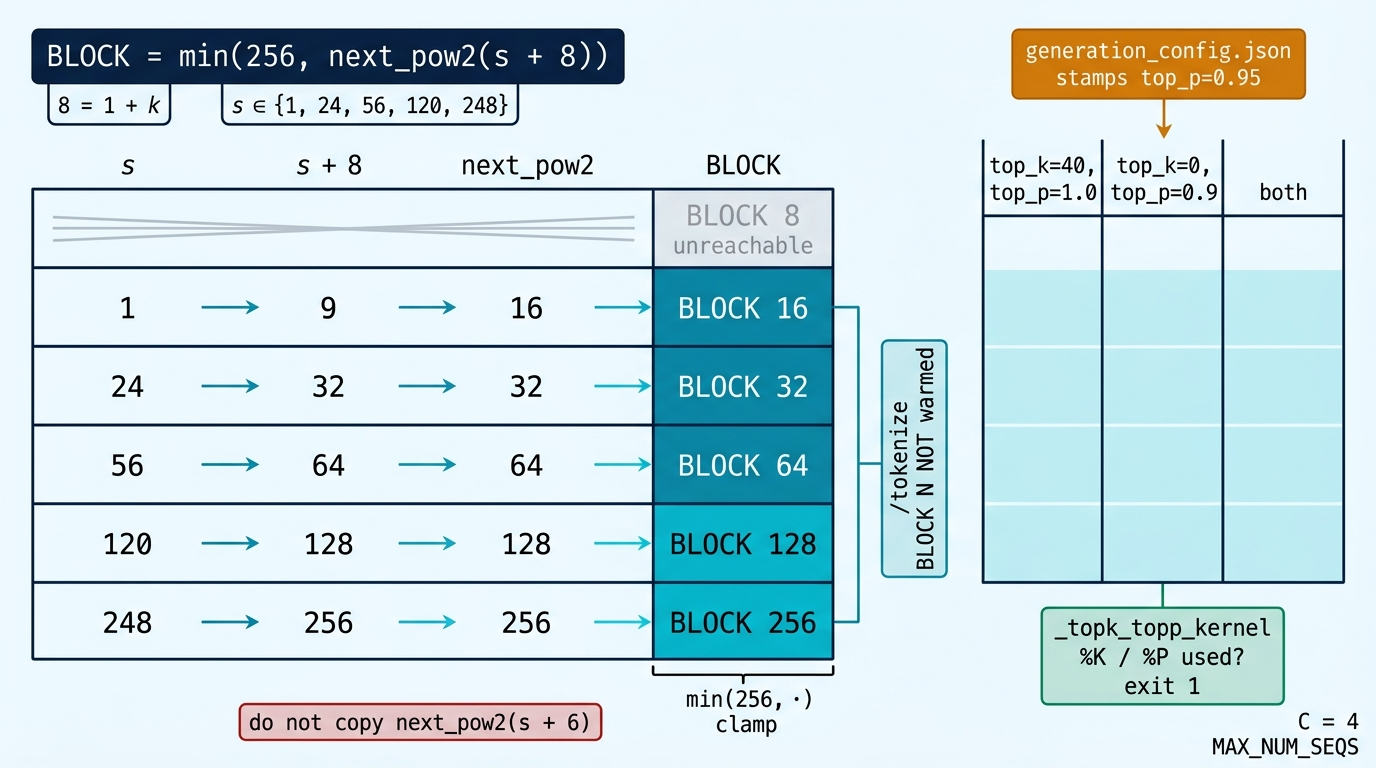
\includegraphics[width=\textwidth]{figures/ch15-warmup-ladder.png}
\caption{The warmup derived from the geometry, not from habit. The DFlash2
attention path's block size is
$\mathrm{BLOCK} = \min(256,\ \mathrm{next\_pow2}(s + 8))$, where $8 = 1 + k$
is the queries per request at $k{=}7$; working backwards, BLOCK 8 is
unreachable because the minimum $s{=}1$ already rounds 9 up to 16, so the live
values are exactly $\{16, 32, 64, 128, 256\}$ and the prompt lengths
$s \in \{1, 24, 56, 120, 248\}$ hit each once. Every rung is checked against
the server's own \code{/tokenize}, because a one-token-off prompt silently
warms the wrong shape. Crossing that ladder is a second dimension no
reasonable warmup would think to cover: the Hub's
\code{generation_config.json} stamps \code{top_p=0.95} onto every request that
does not override it, so three engineered arms are needed to reach all three
Triton kernels --- and the script proves it by grepping the compiled
\code{.ttir} for whether the \code{\%K} and \code{\%P} SSA values are actually
used.}
\label{fig:dflash2-warmup-ladder}
\end{figure}

\section{The bench protocol is the point}
\label{sec:dflash2-bench}

Everything in \Cref{sec:dflash2-fingerprints,sec:dflash2-triton} rests on
one harness being trustworthy, and \repofile{tests/bench_decode.py} earns
that the way \Cref{ch:measurement} taught: by defining its quantity,
salting its inputs, and instrumenting its own blind spots. Every run rides
with its own falsifiers: coherence probes (the capital of France; whether
9.9 exceeds 9.11 --- the classic broken-quant sanity check) and a regex
that scans all output for \code{nan} and for \code{locklock} --- a
fingerprint string of one specific past corruption mode, a named falsifier
for a known ghost. The definition sits at the top of the file: decode \tokspersec{} is
$(\mathrm{completion\ tokens} - 1) / (\mathrm{end} - \mathrm{first\ token\
time})$ --- TTFT excluded, the first token excluded from the rate. The two
phases are fixed prompts: structured is ``Count from 1 to 200. Output only
the numbers\dots'' (with a 32-token warmup run recorded separately, so the
first measurement never pays a JIT or cache miss); prose is the hash-map
explanation. All requests run temperature 0, \code{top_p} 1, streaming with
usage, thinking off; the canonical README protocol is median of 5 runs at
400 tokens.

Around each run the harness snapshots \code{/metrics} and reports
\emph{deltas} of the \code{vllm:spec_decode_*} counters --- skipping the
\code{_created} timestamp gauges that \Cref{ch:specdecode}'s instrument once
mistook for counters --- and derives the accept ratio, accepted-per-step,
and the seven per-position rates from \code{position="i"} labels. A benchmark
that carries its own falsifiers is the
Part~I measurement discipline, inherited whole; what Part~II adds is the
subject of this chapter --- that the per-position vector those counters
yield is not just a health metric but a \emph{localizing} instrument, sharp
enough to convict an attention mask.

\FloatBarrier

Speculative decoding stops being one number here. A $k{=}7$ block emits
seven, and their shape is positional evidence about specific machinery:
position~0 answers for the anchor alone, while positions 1--6 answer for
the taps, the mask, and the edge scores that give the block an interior.
Once that vector is legible, a 2$\times$ throughput collapse is no longer a
performance problem to profile but a fault with an address --- and the
drafter itself stops reading as an appendage bolted onto the target model
and starts reading as a tenant, one that has to be housed inside somebody
else's block pool and warmed on somebody else's launch shapes before it
earns its first token.

\section*{Takeaways}

\begin{itemize}
  \item DFlash2 is the anti-DSpark: a separate Qwen3-architecture drafter
    at $k{=}7$ that brackets every layer in grouped dynamic convolutions
    and decodes one Viterbi-style path through a candidate lattice in a
    single Triton kernel. Position-gated taps and \code{is_causal: false}
    seal that draft block into an 8-slot frame --- which is exactly why the
    block dies wholesale when a causal mask is imposed on it.
  \item Structured decode runs 2.4$\times$ faster than prose on identical
    hardware, weights, and step cost; the spread is pure acceptance. So
    read the \emph{vector}, not the ratio: flat-and-high is a cooperative
    domain, geometric decay from a healthy position 0 is domain entropy
    rather than a fault, uniform depression says the drafter's inputs are
    wrong, and a healthy position 0 over a dead tail says the intra-block
    machinery has been severed.
  \item The fingerprint convicted TRITON\_ATTN without a profiler:
    positions 1--6 dead was the signature of a causal-in-block draft mask,
    worth structured decode falling from 65.1 to $\approx$29 \tokspersec{}
    at 0.31 acceptance. Leave the draft backend unset.
  \item Padded slot-share houses the drafter inside the MLA pool at zero
    added bytes, co-owning MLA tensors at disjoint block ids --- dropping a
    $\approx$36k-token session's KV peak from 44.6\,\% to $\approx$16\,\%
    and unlocking the 1M default context.
  \item Derive a procedure from the geometry, then check its postcondition:
    the block formula yields exactly five live JIT shapes, and only
    engineered sampler arms reach all three Triton kernels --- proved by
    grepping the compiled \code{.ttir} --- just as a benchmark you will
    hang diagnoses on carries salted prompts, coherence probes, and a
    NaN/corruption regex on every run.
\end{itemize}

\chaptertransition{Padded slot-share housed the drafter for zero bytes by
proving it needed none, which raises the same question about every other
reservation in the process --- and one of them answers badly. A single boot
line reports a workspace resized from nothing to 5036.40\,MB: five
gigabytes taken out of the KV pool before a token is served, for a buffer
sized in raw tokens but consumed in 4:1-compressed pools. The next chapter
takes those bytes back not by tuning the number down but by proving what
the allocation can legally be asked for --- and then follows the same
byte-consciousness somewhere no allocator can reach, to roughly twenty
bytes of prompt header whose disappearance re-prefilled a 21{,}642-token
context from scratch.}

% =============================================================================
% Chapter 16 — Bytes by Proof: Workspace Right-Sizing and the Prefix-Cache
% Interface
% =============================================================================

\chapter{Bytes by Proof: Workspace Right-Sizing and the Prefix-Cache Interface}
\label{ch:bytes-by-proof}

A Stage~A boot of 2026-09-01, run with \envvar{VLLM_DEBUG_WORKSPACE=1},
printed one line from the sparse-indexer prefill path: \code{Resized
workspace ... 0.00 MB -> 5036.40 MB}. Five gigabytes, requested during the
memory profile --- subtracted from the KV pool before a single token is
served, and locked for the life of the process --- for a buffer the indexer
can never fill. A units mismatch had sized it in raw tokens where it is
consumed in 4:1-compressed pools: at least ten times anything it can use.

\Cref{ch:perf} taught a discipline of \emph{measured} byte budgets: walk the
checkpoint's shapes, price every decode step in gigabytes streamed, and let the
model of the machine veto folklore tuning. The GLM kit inherits that discipline
and then goes one step further. Where the DeepSeek recipe budgeted bytes by
measuring them, this recipe reclaims them by \emph{proving} them --- it computes
the legal maximum an allocation can ever need, demonstrates by exhaustion that
serving behavior cannot change, and only then flips the knob. The flagship case
returns 4.4--4.85\,GiB of KV pool from that single mis-sized workspace without
touching a kernel. The review that shipped it rejected a faster-looking
tuned alternative precisely because it was a guess rather than a bound.

The second half of the chapter extends the same byte-consciousness to a place
Part~I never had to look: the prompt itself. On a serve whose prefix cache only
counts block-aligned hits at a 3{,}584-token page, every byte of the rendered
prompt is part of the performance interface --- a one-line conditional in a chat
template silently turned every thinking toggle into a full re-prefill of a
21{,}642-token context. The two stories --- and a closing pair of guards,
one against starvation of the shared step budget and one against corruption
across the shared block pool --- define this chapter's doctrine: on
memory-starved hardware, treat allocations as theorems and prompt bytes as
ABI.

For an inference engineer, the payoff is a reusable standard of evidence.
Every serving stack carries reservations someone once sized conservatively
and nobody has re-derived since, and every page-granular cache makes prompt
rendering a performance contract whether or not anyone wrote it down. The
worked examples here --- a boot receipt reconciled to the byte, a
legal-maximum formula, an equivalence test with a demonstrated failure mode,
a template pinned as a strict string extension --- show what it takes to
reclaim such bytes with zero behavioral risk rather than low risk.

\section{From measured budgets to proven ones}
\label{sec:proof-framing}

A measured budget answers ``how much does this cost today?''; a
\emph{proved} budget answers ``what is the largest value this allocation
can legally be asked for, under any input the scheduler is allowed to
construct?'' When the answer is far below what the code reserves, the gap
can be reclaimed with zero behavioral risk --- not low risk, zero ---
provided the proof is real and a guard makes its assumptions fail closed
when the surrounding code drifts. Every section that follows is a worked
example of that pattern at a different scale: 5\,GB, 2.6\,GiB, one
3{,}584-token cache page, and finally about twenty bytes of prompt header.

\section{The five-gigabyte discovery}
\label{sec:proof-workspace}

\subsection{A boot receipt, reconciled to the byte}

Before anyone touched code, the number in the boot line was reconciled
exactly:

\begin{lstlisting}
[WORKSPACE DEBUG] Resized workspace ... 0.00 MB -> 5036.40 MB (ubatch 0)
\end{lstlisting}

vLLM's \code{get_max_prefill_buffer_size} returns
\code{max_model_len * 40} entries, each entry 132 bytes (128 bytes of fp8
values plus a 4-byte scale). At the kit's \code{max_model_len} of
1{,}000{,}000 that is 40{,}000{,}000 entries, and
$40{,}000{,}000 \times 132 + 1\,\text{MiB}$ of radix top-$k$ scratch is
5{,}281{,}048{,}576 bytes --- which formats to exactly ``5036.40\,MB''. The
host test suite (\repofile{tests/test_indexer_workspace.py}, 819 lines) pins
that reconciliation as \code{test_stock_matches_live_workspace_receipt}: the
sizing formula must reproduce the logged receipt to the digit, or the model of
the allocation is wrong and nothing downstream of it can be trusted.

\subsection{Sized in tokens, indexed in pools}

Why is the buffer an order of magnitude larger than anything the indexer can
use? The
design note \repofile{docs/DESIGN-indexer-workspace.md} (PR~86, contributed by
nood-co1) traces it to a units mismatch. GLM-5.3-Flash's sparse indexer
compresses keys into pools: \code{compress_ratio == index_kpool == 4}, so the
metadata builder hands the prefill splitter sequence lengths that are already
divided by four. The workspace that backs the splitter's gather, however, is
sized from \emph{raw token counts}. Upstream's sibling call site in
\code{deepseek_v4/attention.py} already divides by \code{compress_ratio}
before sizing; the \code{glm5next/nvidia/attention.py} call site does not ---
in the design note's words, ``the 4$\times$ is the whole of the gap between the
two call sites.'' The workspace is sized in tokens where it is indexed in
pools (\Cref{fig:proof-tokenspools}).

The same un-divided ratio surfaced a
second time in the review: a decode-logits pitch that over-strides by a flat
4$\times$ --- the same \emph{class} of bug at a second call site, confirmed
real by the Codex review. The review then \emph{declined to fix it} in the
same PR because its safety case was unproven: the 128-byte alignment
contract had not been established against the SM120 paged-MQA kernel, and
the op is captured inside the full CUDA graph, so it needs its own
kernel-ABI gate.
Leaving a confirmed bug outside the proof's perimeter is the same scoping
discipline that rejected the tuned REQS${=}8$ sizing
(\Cref{sec:proof-rightsizing}) --- and spotting the repeated class is
exactly what \Cref{ch:perf}'s cost-model habit exists to catch.

\begin{figure}[htbp]
\centering
\adjustbox{max width=\textwidth}{%
\begin{tikzpicture}[node distance=7mm and 9mm,font=\small]
  \node[hbnode] (cfg) {\texttt{max\_model\_len}\\$1{,}000{,}000$ tokens\\compress ratio 4};
  \node[hbbox,above right=1mm and 10mm of cfg] (dsv)
    {\texttt{deepseek\_v4} call site\\sizes with seq lens $\div$ 4};
  \node[hbwarn,below right=1mm and 10mm of cfg] (glm)
    {\texttt{glm5next} call site\\forgets the $\div$ 4};
  \node[hbgpu,right=of dsv] (ok)
    {workspace in POOLS\\matches what the\\splitter consumes};
  \node[hbwarn,right=of glm] (bad)
    {workspace in TOKENS\\$1\text{M} \times 40 = 40{,}000{,}000$ entries\\= 5036.40\,MB locked};
  \node[hbfaint,below=9mm of bad,xshift=-14mm] (consumer)
    {splitter actually consumes\\\texttt{seq\_lens // 4} (pools)};
  \draw[hbok] (cfg) -- (dsv);
  \draw[hbfail] (cfg) -- (glm);
  \draw[hbok] (dsv) -- (ok);
  \draw[hbfail] (glm) -- (bad);
  \draw[hbarrow,dashed] (consumer) -- (bad)
    node[hblabel,midway,anchor=west,xshift=1mm] {10$\times$ oversized at seqs=16};
  % scale bars: 1 cm per ~500 MB
  \begin{scope}[shift={(0,-4.6)}]
    \fill[hbAccent!25] (0,0) rectangle (10.07,0.55);
    \draw[hbSteel,thick] (0,0) rectangle (10.07,0.55);
    \node[font=\scriptsize] at (5.0,0.28) {stock: 5036.40\,MB locked at boot};
    \fill[hbGreen!30] (0,-0.95) rectangle (1.01,-0.4);
    \draw[hbSteel,thick] (0,-0.95) rectangle (1.01,-0.4);
    \node[hblabel,anchor=west] at (1.15,-0.68)
      {rightsize: 503.5\,MiB at seqs=16 (125.9\,MiB at the default seqs=4)};
    \node[hblabel,anchor=north west] at (0,-1.35)
      {both drawn to scale; the difference returns to the KV pool};
  \end{scope}
\end{tikzpicture}%
}
\caption{The tokens-versus-pools sizing bug. The sparse indexer gathers over
\emph{pools} (keys compressed 4:1), and the upstream \code{deepseek_v4} call
site divides by the compression ratio before sizing its workspace. The
\code{glm5next} call site does not, so the prefill gather workspace is sized
from raw token counts: $1\text{M} \times 40$ entries at 132 bytes each,
5036.40\,MB reserved during the memory profile and locked for the life of the
process.}
\label{fig:proof-tokenspools}
\end{figure}

\section{Right-sizing by legal maximum, not tuned guess}
\label{sec:proof-rightsizing}

\subsection{The shipped formula}

The expression below is short, and every symbol in it is load-bearing; the
paragraph that follows takes the factors one at a time. What makes it a bound
rather than a setting is that every rounding in it runs in the direction that
cannot under-size.

The fix, \repofile{overlay/patch_indexer_workspace.py}, does not pick a
comfortable number. It computes the provable per-step maximum:

\begin{equation*}
\text{entries} \;=\; \min(\text{max\_num\_seqs},\, \text{MNBT})
\;\times\; \left\lceil
\frac{\text{max\_model\_len} + k}{\text{compress\_ratio}} \right\rceil
\end{equation*}

Each factor is an argument, not a preference. The $\min$ bounds how many
prefill requests one step can carry, because every prefill row costs at least
one query token of the \code{max_num_batched_tokens} budget. The $+k$ term
(the drafter's seven speculative tokens, \Cref{ch:dflash2}) covers the scheduler's
\code{seq_lens_cpu_upper_bound}, which speculation can push past
\code{max_model_len} --- the host tests show the size growing by exactly
$2 \times 16 = 32$ entries when $k{=}7$ rolls the ceiling division over. And
the division is a ceiling, not a floor, because the consumer floors
(\Cref{fig:proof-legalmax} takes the formula factor by factor).

At the live configuration ($M{=}10^6$, ratio 4, \code{max_num_seqs}${=}16$,
MNBT${=}2048$, $k{=}7$) this yields
$\lceil (1{,}000{,}000+7)/4 \rceil = 250{,}002$ compressed entries per request
and $250{,}002 \times 16 = 4{,}000{,}032$ entries total ---
528{,}004{,}224 bytes, 503.5\,MiB against the stock 5035.4\,MiB. The tests
bound the reclaim at 4.40--4.45\,GiB at seqs${=}16$; at the recipe's shipped
\code{MAX_NUM_SEQS=4} the workspace shrinks to 125.9\,MiB and the reclaim to
4.75--4.85\,GiB. The design note prices the result as roughly
\textbf{+26--28\,\% KV-pool capacity}, and the acceptance criterion is
characteristically literal: capacity is read from the allocator's own startup
lines, never from GiB arithmetic on paper
(\Cref{tab:proof-reclaims}).

\begin{table}[htbp]
\centering
\small
\caption{Memory reclaimed by proof rather than tuning (all figures from the
repository's dated receipts; workspace receipt 2026-09-01).}
\label{tab:proof-reclaims}
\begin{tabular}{@{}>{\raggedright\arraybackslash}p{4.1cm}rr>{\raggedright\arraybackslash}p{4.6cm}@{}}
\toprule
Allocation & Stock & Proved need & Reclaimed \\
\midrule
Indexer prefill workspace, seqs=16 & 5036.40\,MB & 503.5\,MiB &
  4.40--4.45\,GiB ($\approx$+26--28\,\% KV pool) \\
Indexer prefill workspace, seqs=4 (shipped default) & 5036.40\,MB &
  125.9\,MiB & 4.75--4.85\,GiB \\
CUDA-graph memory estimate (\envvar{CG_ESTIMATE=0}, PR~25) & 2.43\,GiB
  reserved & $-0.19$\,GiB measured & $\approx$2.6\,GiB \\
\bottomrule
\end{tabular}
\end{table}

\subsection{The review that rejected a faster guess}

The first draft of the patch carried a tuned knob: size the workspace for
\code{REQS=8} concurrent prefills, 2{,}000{,}000 entries, a tidy 264\,MB.
The adversarial Codex review rejected it with a one-line verdict --- ``a
throughput tradeoff, not the required workspace'' --- and the test suite now
contains the proof of why. Under the REQS${=}8$ sizing, a legal batch of
sixteen 1M-context thin prefills no longer fits in one workspace pass: the
splitter breaks it into \emph{two} chunks and re-runs
\code{cp_gather_indexer_k_quant_cache}, changing serving behavior in a way no
one measured. The shipped default is the legal maximum precisely so that the
constraint \code{new_n <= workspace_size} can never bind where stock's did
not.

That no-behavior-change claim is then checked rather than asserted. The patch
carries a host replica of vLLM's own \code{split_prefill_chunks}, and
\code{test_chunking_is_identical_to_stock} replays 400 randomly generated
\emph{legal} batches (seeded \code{random.Random(20260901)}) plus
deterministic extremes, requiring byte-identical chunk lists under stock and
right-sized workspaces. It also requires that the sweep exercised at least
one multi-chunk batch, ``or it proves nothing about chunking at all.'' A companion
power test proves the equivalence test \emph{can} fail: it feeds the rejected
REQS${=}8$ sizing through the same machinery and watches the chunk list split.
An equivalence test without a demonstrated failure mode is a tautology; this
one has teeth.

\begin{figure}[htbp]
\centering
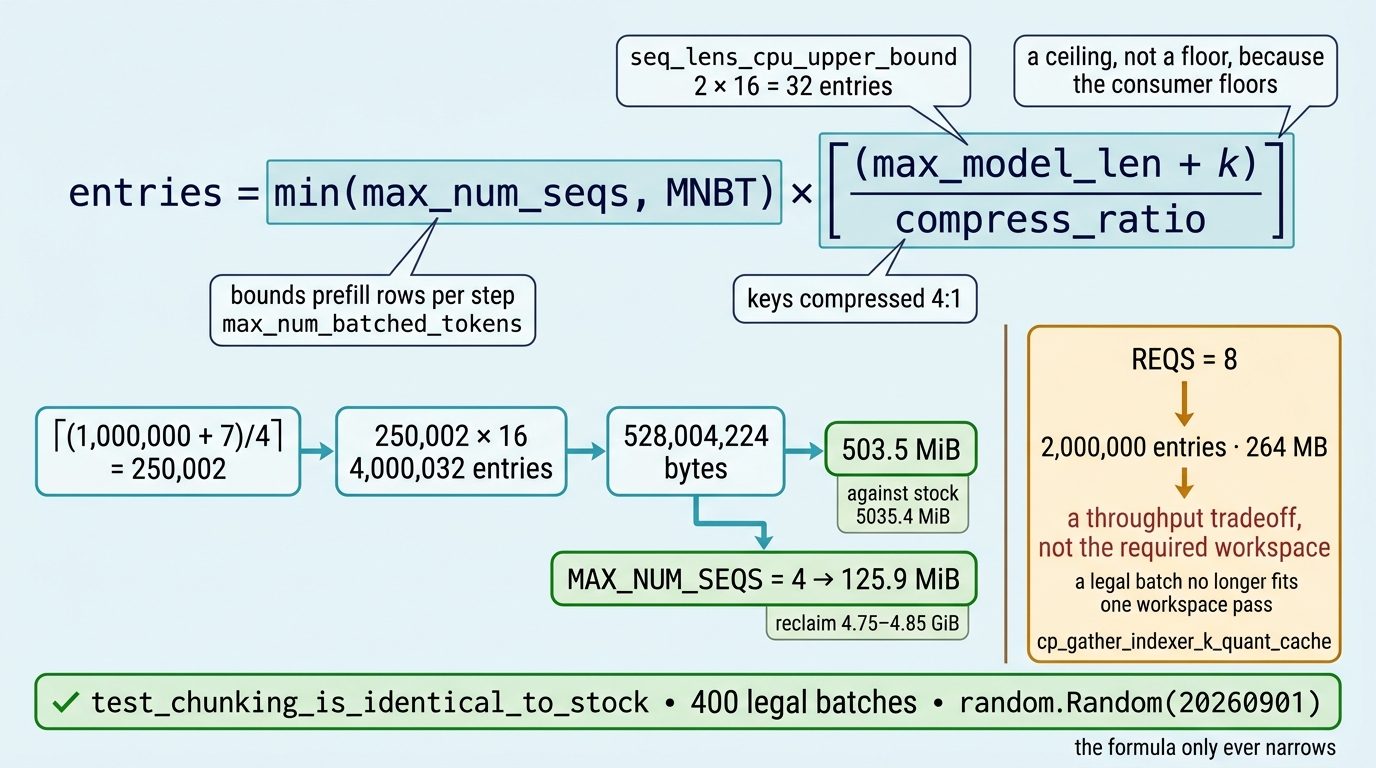
\includegraphics[width=\textwidth]{figures/ch16-legal-maximum.png}
\caption{The shipped formula, factor by factor. The $\min$ bounds how many
prefill requests one step can carry, because every prefill row costs at least
one query token of the \code{max_num_batched_tokens} budget; the $+k$ covers
the scheduler's \code{seq_lens_cpu_upper_bound}, which the drafter's seven
speculative tokens can push past \code{max_model_len}; and the division is a
ceiling rather than a floor because the consumer floors. At the live
configuration this yields 250{,}002 compressed entries per request and
4{,}000{,}032 in total --- 528{,}004{,}224 bytes, 503.5\,MiB against the stock
5035.4\,MiB, and 125.9\,MiB at the shipped \code{MAX_NUM_SEQS=4}. The first
draft's tuned \code{REQS=8} sizing was rejected as ``a throughput tradeoff,
not the required workspace'': under it a legal batch of sixteen 1M-context
thin prefills no longer fits in one workspace pass.
\code{test_chunking_is_identical_to_stock} replays 400 randomly generated
legal batches to prove the shipped sizing changes nothing, and a companion
power test proves the equivalence test can fail.}
\label{fig:proof-legalmax}
\end{figure}

\begin{hblesson}
When reclaiming a reservation, compute the legal maximum, never a tuned
estimate. A tuned number trades an invisible amount of behavior for memory and
must be re-measured on every geometry change; a legal maximum is a theorem
about the code, valid until the code changes --- at which point a fail-closed
guard should turn the invalidated assumption into a boot error instead of a
silent under-size. And pair every ``nothing changed'' equivalence test with a
power test proving the test can detect a change, or the equivalence claim is
untestable by construction.
\end{hblesson}

\subsection{An enum, because a typo must not pick a serving mode}

Activation is deliberately rigid. \envvar{GLM53_INDEXER_WORKSPACE} accepts
exactly two literal strings, \code{stock} (the default; unset means stock,
byte-for-byte the original expression) and \code{rightsize}. Everything else
--- \code{""}, \code{" rightsize "}, \code{RIGHTSIZE}, \code{1}, \code{on},
\code{right-size} --- is rejected at launch, on the grounds the launcher
comment states outright: ``a typo'd knob must not silently pick a serving
mode.''

The rule has a scar. PR~38 (hecisaza's numeric-knob
validation) landed after a \envvar{GPU_MEM_UTIL=8.7} typo took down a
healthy two-node deployment before being diagnosed: \code{./start.sh
restart} calls \code{stop} before vLLM can even parse the bad value, so the
typo killed a working serve rather than being rejected by it. Hence
validate-before-dispatch --- \code{validate_numeric_config()} now runs
before the restart is allowed to touch anything, and the byte-literal enum
here inherits the same posture.

The same accept/reject set is implemented twice, once in the bash
launcher's \code{_glm53_validate_enum} and once in the Python patch. A
test executes \emph{both} implementations over the same value list and diffs
their verdicts value-for-value, so a knob cannot change meaning across the
container boundary. Even the rejected result is clamped: the formula only ever
narrows, and a configuration whose legal maximum exceeds stock keeps stock and
logs the upstream latent risk instead of pretending to fix it.

\section{The guard that guarded the wrong case}
\label{sec:proof-guard}

A proof is only as durable as the guard that watches its assumptions, and
the guard is where this patch earned its scar: the first draft of its
fail-closed cross-check carried a conditional that read as an optimization
and was, in fact, a hole. The story is best told as it unfolded.

\begin{hbwarstory}
The right-sizing patch shipped with a fail-closed cross-check --- and the first
draft of that cross-check contained the chapter's best bug. The sizing formula
can only read \code{hf_text_config.index_kpool}; the authoritative runtime
value, \code{kv_cache_spec.compress_ratio}, resolves later, in the metadata
builder's \code{__init__}. ``Same number by construction, but construction is
not a check,'' so the patched builder compares them at init on every TP rank.
The PR~8 draft wrote the comparison as:

\begin{lstlisting}[language=Python]
# PR-8 draft -- rejected by review as a blocker
if mode == "rightsize" and self.compress_ratio > 1:
    ...cross-check...

# shipped form -- unconditional, both directions
if mode == "rightsize":
    ...raise on any index_kpool/compress_ratio mismatch...
\end{lstlisting}

The \code{compress_ratio > 1} clause looks like a harmless optimization ---
uncompressed models have nothing to cross-check. It skips exactly the one
combination that under-sizes: \code{index_kpool=4} in the config with a
runtime \code{compress_ratio} of 1. In that state the workspace is sized for
compressed pools (4{,}000{,}032 entries) while the runtime hands the splitter
raw token counts. The worst case is $16 \times 1{,}000{,}007 \approx 16$M
entries, which the regression test asserts is more than $3.9\times$ the sized
workspace: ``$\sim$4x under-sized, uncaught.'' The Codex review flagged it as
a blocker; the shipped guard raises unconditionally, in both mismatch
directions, naming \code{index_kpool}, \code{compress_ratio}, and the env var
in the error. Direction B --- config says uncompressed, runtime compresses ---
cannot under-run, but ``the two config sources disagree about the model and
rightsize must not serve on that.''
\end{hbwarstory}

The lockdown that followed is as instructive as the bug. The test suite pins
the fix three ways: \code{test_builder_ratio_mismatch_raises_both_directions}
exercises \emph{both} mismatch directions behaviorally;
\code{test_builder_guard_has_no_ratio_condition} pins the \emph{source form},
asserting the shipped guard text no longer contains the old
\code{if _glm53_workspace_mode() == "rightsize" and self.compress_ratio}
conditional --- because behavioral tests alone could pass against a merely
reordered guard; and the builder additionally raises if the allocated
workspace is ever below the legal per-step maximum, so a future resize in
either direction trips the same wire. A guard that skips its worst case is
worse than no guard, because it converts ``we don't check'' into ``we
checked.'' The review treated that as a blocker, and the tests make the
mistake unrepeatable --- \Cref{fig:proof-guardcell} shades the cell the
condition skipped.

\begin{figure}[htbp]
\centering
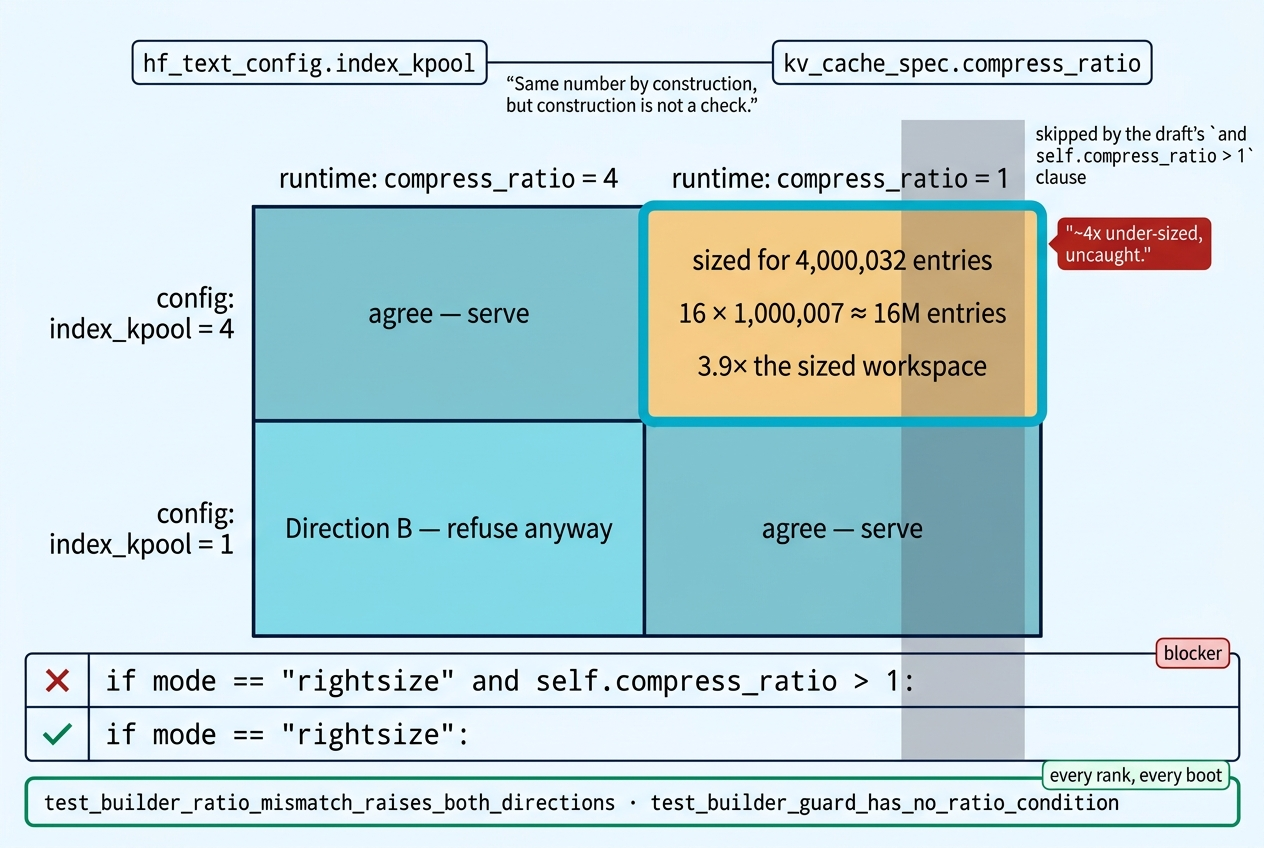
\includegraphics[width=\textwidth]{figures/ch16-guard-cell.png}
\caption{The four states of a two-source cross-check. The sizing formula can
only read \code{hf_text_config.index_kpool}, while the authoritative
\code{kv_cache_spec.compress_ratio} resolves later in the metadata builder's
\code{__init__} --- ``same number by construction, but construction is not a
check.'' The PR~8 draft guarded the comparison behind
\code{self.compress_ratio > 1}, which reads as a harmless optimisation and in
fact shades out the entire right-hand column, including the one cell that
under-sizes: config says pools, runtime hands raw token counts, and a worst
case of $16 \times 1{,}000{,}007 \approx 16$M entries meets a workspace sized
for 4{,}000{,}032 --- over $3.9\times$ under. The shipped guard raises
unconditionally in both directions, on every rank at every boot, and three
tests pin it: two behavioural, one on the source form itself, because a
behavioural test alone could pass against a merely reordered guard.}
\label{fig:proof-guardcell}
\end{figure}

\section{Smaller reclaims, same doctrine}
\label{sec:proof-smaller}

The same doctrine operates at a second scale, one order of magnitude down.
vLLM subtracts a CUDA-graph memory \emph{estimate} from the KV pool before
capture. On this kit the estimate is 2.43\,GiB, while the captured graphs,
once measured, actually consumed $-0.19$\,GiB --- at or below zero net. The
2.43\,GiB deduction was pure pessimism: roughly 2.6\,GiB of KV reserved and
never used. PR~25's
\envvar{CG_ESTIMATE=0} keeps CUDA graphs fully on and drops only the
deduction: again, not a tuning knob but the replacement of a pessimistic guess
with a measured actual, reclaiming capacity with no change to what executes.
The estimator anomaly and the workspace sit on the same ledger in
\Cref{tab:proof-reclaims}. Between them, the two dated boot receipts bracket
the pool's growth: the 2026-08-28 serve booted a 1{,}754{,}237-token KV
pool, and the 2026-09-01 validated boot (MNBT 7168, the E2 prefill kernel, and
\code{rightsize} together) reports 1{,}243{,}902 tokens at a different
geometry --- each quoted from the allocator's own startup lines rather than
derived arithmetic.

The habit of cross-checking one value from two sources, in both directions,
also outlived the guard that taught it: the shipped builder init verifies
\code{index_kpool} against \code{compress_ratio} on every rank at every boot,
unconditionally. On this recipe, an assumption a proof depends on is never
checked once at patch time --- it is re-verified at every boot, on every rank,
and a disagreement refuses to serve. Every byte reclaimed this way lands in
the KV pool; whether prompts can actually \emph{reuse} that pool is the
question the rest of the chapter turns to.

\section{The prefix cache is page-quantized}
\label{sec:proof-prefixpage}

\subsection{Only whole pages count}

The second half of the byte story begins with a fact about the KV layout from
\Cref{ch:quantized-bet}'s hybrid geometry: the sparse-MLA \code{KpoolTailManager} disables
fine-grained prefix-cache hits, so only \emph{block-aligned} tokens count, and
the alignment is the 3{,}584-token hybrid MLA page. A warm prompt reuses
exactly $\lfloor \text{tokens} / 3584 \rfloor \times 3584$ tokens --- nothing
in between. The consequences are counter-intuitive enough that the repository built
a bench around them (\Cref{fig:proof-pagehits}): a 6.8k-token conversation
reuses \emph{one} page (3{,}584 tokens, roughly 53\,\% of its prompt), while a
7.7k conversation reuses two (7{,}168 tokens, roughly 93\,\% --- ``the
upstream headline''). Two prompts a mere 900 tokens apart in length sit forty
percentage points apart in reuse, because one of them crosses a page boundary
and the other does not. The practical form of this is that prompt length buys
reuse in steps rather than in proportion: the token that completes a page is
worth 3{,}584 tokens of recomputation, and the one after it is worth nothing
until 3{,}583 more arrive.

\begin{figure}[htbp]
\centering
\adjustbox{max width=\textwidth}{%
\begin{tikzpicture}[font=\small]
  % scale: 0.9 mm per 100 tokens -> 0.9 cm per 1000 tokens
  \def\ppx#1{#1*0.09}
  % page boundary grid
  \foreach \b/\lab in {0/0, 35.84/3584, 71.68/7168, 107.52/10752} {
    \draw[hbSteel!50,dashed] (\ppx{\b},0.4) -- (\ppx{\b},-3.3);
    \node[hblabel,anchor=south] at (\ppx{\b},0.45) {\lab};
  }
  \node[hbtitle,anchor=south west] at (\ppx{0},1.0)
    {3584-token page boundaries (block-aligned hits only)};
  % prompt A: 6.8k
  \fill[hbGreen!35] (0,-0.5) rectangle (\ppx{35.84},-1.15);
  \fill[hbGray]    (\ppx{35.84},-0.5) rectangle (\ppx{68},-1.15);
  \draw[hbSteel,thick] (0,-0.5) rectangle (\ppx{68},-1.15);
  \node[hblabel,anchor=west] at (\ppx{68}+0.15,-0.82)
    {6.8k prompt: 1 full page = 3584 hit tokens ($\approx$53\,\%)};
  % prompt B: 7.7k
  \fill[hbGreen!35] (0,-1.75) rectangle (\ppx{71.68},-2.4);
  \fill[hbGray]    (\ppx{71.68},-1.75) rectangle (\ppx{77},-2.4);
  \draw[hbSteel,thick] (0,-1.75) rectangle (\ppx{77},-2.4);
  \node[hblabel,anchor=west] at (\ppx{77}+0.15,-2.07)
    {7.7k prompt: 2 full pages = 7168 hit tokens ($\approx$93\,\%)};
  % legend
  \fill[hbGreen!35] (0,-3.05) rectangle (0.4,-2.75);
  \node[hblabel,anchor=west] at (0.5,-2.9) {reused (cache hit)};
  \fill[hbGray] (3.6,-3.05) rectangle (4.0,-2.75);
  \node[hblabel,anchor=west] at (4.1,-2.9) {recomputed (below the next boundary)};
\end{tikzpicture}%
}
\caption{Page-quantized prefix reuse. The hybrid KV layout counts hits only in
whole 3584-token MLA pages: a 6.8k-token warm prompt reuses one page
($\approx$53\,\% hit ratio) while a 7.7k prompt reuses two ($\approx$93\,\%).
\repofile{tests/bench_prefix_cache.py} scores measured hits against this page
model as \code{hit_efficiency} and defaults to 8{,}400 prompt tokens so its
warm turn crosses the second boundary.}
\label{fig:proof-pagehits}
\end{figure}

\subsection{A bench that scores itself against the model}

\repofile{tests/bench_prefix_cache.py} makes the page model executable. Each
run stages a cold turn (system prompt plus a long unique document) and a warm
follow-up that resends the identical history, reading
\code{vllm:prefix_cache_hits} and \code{queries} counter deltas around each
turn. Its headline metric is not the raw hit ratio but
\code{hit_efficiency}: measured hit tokens divided by the full-page
expectation $\lfloor \text{tokens}/3584 \rfloor \times 3584$. A value of 1.0
means the page model is being respected; the tool warns when the median falls
below 0.9, meaning either the warm prompt fails to cross a full page boundary
or reuse is partial. The default \code{--prompt-tokens 8400} is chosen to land
about 8.1k measured tokens --- safely across the second boundary --- so an
out-of-the-box run exercises a two-page hit rather than teetering on one
(\Cref{tab:proof-hits}).

\begin{center}
\small
\captionof{table}{The 3584-token page model against measured reuse. Model
rows follow $\lfloor\text{tokens}/3584\rfloor \times 3584$; the measured row
is the 2026-08-29 cold-prefill ladder's APC follow-up receipt.}
\label{tab:proof-hits}
\begin{tabular}{@{}rrrr>{\raggedright\arraybackslash}p{4.0cm}@{}}
\toprule
Prompt tokens & Full pages & Hit tokens & Hit ratio & Note \\
\midrule
6{,}800 & 1 & 3{,}584 & $\approx$53\,\% & below the second boundary \\
7{,}700 & 2 & 7{,}168 & $\approx$93\,\% & ``the upstream headline'' \\
8{,}004 & 2 & 7{,}168 & 89.6\,\% & measured: warm TTFT 1.30\,s after a
  10.36\,s cold (2026-08-29) \\
14{,}336 & 4 & 14{,}336 & 100\,\% & exactly four pages \\
\bottomrule
\end{tabular}
\end{center}

\subsection{Cold means salted: the 5$\times$ TTFT swing}

The page model also explains why this repository's cold benchmarks are paranoid.
This vLLM build exposes no cache-reset endpoint, so a ``cold'' measurement is
only cold if no previous session cached its pages. On 2026-08-29 two bench
sessions disagreed by $5\times$ on cold TTFT; the reruns had reused chat
content, and the supposedly cold turn dropped from 10.3\,s to 1.9\,s on
recycled pages. The fix is baked into the harnesses rather than into
operator discipline. \repofile{tests/bench_prefix_cache.py} injects a
per-invocation session salt into every checksum string of its filler
document, and the cold-prefill ladder
(\repofile{tests/_run_cold_prefill.py}, protocol in
\repofile{docs/cold-prefill.md}) puts a unique UUID-plus-hex-pad salt
\emph{first} in every user message so the prefix cache cannot cheat. Both
instrument their own cold turns with per-request metric deltas
(\code{prefix_cache_hits_total},
\code{prompt_tokens_by_source_total\{source="local_compute"\}}), so a cold
rung that actually hit cache is self-incriminating --- the same
distrust-your-own-benchmark reflex \Cref{ch:measurement} institutionalized, now applied
to a cache that never forgets.

\needspace{5\baselineskip}
\section{Prompt bytes as a performance interface}
\label{sec:proof-pr63}

\subsection{The PR~63 story: a one-line guard, a full re-prefill}

The page model has a corollary the lab learned the expensive way: the bytes
at the very head of a prompt hold every page behind them hostage.

\begin{hbwarstory}
vLLM chains prefix-cache block hashes forward from token 0, and on this serve
only whole 3{,}584-token pages count. So any divergence near the head of the
prompt invalidates \emph{everything} behind it. The kit's chat template
rendered a \code{<|system|>Reasoning Effort: X} header at the very start of
the prompt --- but gated it on \code{thinking_enabled}. Toggle thinking off,
and the header disappears: the thinking-on and thinking-off renderings of the
same conversation diverge at roughly token~2. With tools present --- and agent
traffic always carries tools --- the two prompts shared 22 characters out of
855. Every thinking toggle therefore re-prefilled the world. Measured on a
21{,}642-token prompt, toggling reasoning effort high$\to$none cost a full
cold prefill, 26.54\,s; after the fix, the same toggle completed in
0.42\,s warm. The fix (PR~63, contributed by sovereignbrah, commit
\code{4753ac2}: ``emit Reasoning Effort unconditionally to keep the prefix
cache'') is one line of template logic --- and it also restores the upstream
zai-org template's behavior, which the guard had quietly forked.
\end{hbwarstory}

The repaired template treats prompt-prefix stability as a tested contract, not
a hope (\Cref{fig:proof-divergence}). \code{<|system|>Reasoning Effort: Max}
is rendered at position 0 of every prompt, in \emph{both} thinking modes.
Thinking is disabled by pre-closing the block, so the generation prompt ends
\code{<|assistant|><think>} when thinking is on and
\code{<|assistant|><think></think>} when it is off. That makes the
thinking-off prompt a \emph{strict string extension} of the thinking-on
prompt, with suffix exactly \code{</think>}.
\repofile{tests/test_chat_template.py} asserts precisely that --- both without
tools and, critically, with tools present, ``because agent traffic always
carries tools; the tools block renders after the reasoning-effort line, so
this is the case that actually regressed.''

The general form is worth extracting: when two renderings of the same
conversation must both hit a page-granular cache, make one a strict extension
of the other rather than a variant of it. Divergence in the tail costs one
page; divergence in the head costs every page behind it.

A further pin holds the effort levels themselves to a shared prefix up to the length of
\code{[gMASK]<sop><|system|>Reasoning Effort: }, so switching Max to Low
diverges as late as the token stream allows. Two pre-existing tests had
\emph{encoded the divergence} as expected behavior; PR~63 rewrote them ---
a reminder that a test suite can canonize a bug as faithfully as it canonizes
a fix.

\begin{figure}[htbp]
\centering
\adjustbox{max width=\textwidth}{%
\begin{tikzpicture}[font=\small]
  % BEFORE panel
  \node[hbtitle,anchor=west] at (0,1.1) {Before PR~63: header gated on thinking};
  % thinking on row
  \node[hblabel,anchor=east] at (-0.15,0.3) {thinking on};
  \fill[hbGreen!35] (0,0) rectangle (0.9,0.6);
  \fill[hbBlue!20] (0.9,0) rectangle (5.6,0.6);
  \fill[hbGray] (5.6,0) rectangle (10.6,0.6);
  \draw[hbSteel,thick] (0,0) rectangle (10.6,0.6);
  \node[font=\scriptsize] at (3.25,0.3) {\texttt{<|system|>Reasoning Effort: Max}};
  \node[font=\scriptsize] at (8.1,0.3) {tools + history (855 chars)};
  % thinking off row
  \node[hblabel,anchor=east] at (-0.15,-0.75) {thinking off};
  \fill[hbGreen!35] (0,-1.05) rectangle (0.9,-0.45);
  \fill[hbAccent!25] (0.9,-1.05) rectangle (10.6,-0.45);
  \draw[hbSteel,thick] (0,-1.05) rectangle (10.6,-0.45);
  \node[font=\scriptsize] at (5.75,-0.75) {header dropped $\rightarrow$ diverges at token 2 (22/855 shared chars)};
  \draw[hbfail] (0.9,-1.3) -- (10.6,-1.3)
    node[hblabel,midway,anchor=north,yshift=-0.5mm]
    {every thinking toggle = full re-prefill: 26.54\,s on a 21{,}642-token prompt};
  % AFTER panel
  \node[hbtitle,anchor=west] at (0,-2.6) {After PR~63: header unconditional, off = strict extension};
  \node[hblabel,anchor=east] at (-0.15,-3.4) {thinking on};
  \fill[hbGreen!35] (0,-3.7) rectangle (9.2,-3.1);
  \draw[hbSteel,thick] (0,-3.7) rectangle (9.2,-3.1);
  \node[font=\scriptsize] at (4.6,-3.4)
    {\texttt{Reasoning Effort: Max} at position 0 + tools + history + \texttt{<think>}};
  \node[hblabel,anchor=east] at (-0.15,-4.45) {thinking off};
  \fill[hbGreen!35] (0,-4.75) rectangle (9.2,-4.15);
  \fill[hbAmber!35] (9.2,-4.75) rectangle (10.6,-4.15);
  \draw[hbSteel,thick] (0,-4.75) rectangle (10.6,-4.15);
  \node[font=\scriptsize] at (4.6,-4.45) {identical prefix, byte for byte};
  \node[font=\scriptsize] at (9.9,-4.45) {\texttt{</think>}};
  \draw[hbok] (0,-5.0) -- (9.2,-5.0)
    node[hblabel,midway,anchor=north,yshift=-0.5mm]
    {shared prefix survives the toggle: 0.42\,s warm};
\end{tikzpicture}%
}
\caption{The token-2 divergence and its repair. Before PR~63 the
reasoning-effort header was gated on \code{thinking_enabled}, so thinking-on
and thinking-off prompts shared only 22 of 855 characters with tools present
and every toggle re-prefilled from scratch (26.54\,s at 21{,}642 tokens).
After the fix the header renders unconditionally at position 0 and the
thinking-off prompt is a strict extension of the thinking-on prompt with
suffix exactly \code{</think>} --- the toggle became a 0.42\,s warm hit.}
\label{fig:proof-divergence}
\end{figure}

\subsection{The client side of the interface}

If prompt bytes are an interface, clients are counterparties, and the repository
ships its reference client configuration under \repofile{examples/pi/} --- a
throughput-honest budget for pointing a coding agent at this serve. The Pi
configs hard-wire \code{chat_template_kwargs} with \code{enable_thinking}
false, so every agent request rides the exact thinking-off template shape the
prefix-stability tests pin. They cap the client's \code{contextWindow} at
500{,}000 tokens --- deliberately half the server's 1M
\code{max_model_len} --- and they bound agent concurrency to
\code{maxConcurrent: 2} subagents (one foreground), matched to the recipe's
small \code{MAX_NUM_SEQS}. Two Sparks serving roughly 37 \tokspersec{} per
stream under four-way concurrency cannot feed an unbounded agent swarm, and
the configuration says so in numbers rather than in a warning nobody reads.

\section{Two starvation and corruption guards in the same spirit}
\label{sec:proof-guards}

Two more overlay patches close the chapter, and they bracket the two costs
of sharing one pool of bytes among heterogeneous consumers. The scheduler
shares a token budget and must sometimes refuse to (starvation); the KV
groups share a block pool and must be prevented from writing across each
other (corruption). Each fix is a small, provable intervention at a
precisely identified boundary, shipped with a test that encodes the
incident.

\subsection{The decode floor: refuse to share the step}

Issue \ghissue{6} in the GLM kit's tracker records the symptom: mixed decode
was roughly $11\times$ slower than solo decode. The engine step budget
(1{,}024 tokens at the time) is shared; a decode lane needs about 8 tokens
(one bonus plus the drafter's $k{=}7$), and the leftover $\sim$1{,}016 went to
a peer's sparse-MLA cold-prefill chunk costing $\sim$1.5\,s per step. Decode
still ran --- at $\sim$5 \tokspersec{} instead of $\sim$50. The instinctive
fix, capping mixed prefill at 128 tokens, was tried and was \emph{not
enough}: the sparse indexer carries a large per-step fixed cost, and mixed
decode still crawled at $\sim$10 \tokspersec{} on an 80k-token KV. So
\repofile{overlay/patch_scheduler_decode_floor.py} skips mixed prefill
entirely: while any peer is decoding, waiting prefills are deferred to the
next step and running-queue prefills are capped, resuming at full chunk size
the moment no one decodes. (\envvar{GLM53_MIXED_PREFILL_CHUNK=skip};
\code{N>0} is available as a cap for operators who want to mix anyway.) The live
regression test, \repofile{tests/test_mixed_prefill_decode.py}, decodes one
lane solo, then again while a second lane cold-prefills, and fails at a solo-to-mixed ratio above $5\times$ --- the comment is explicit that $11\times$
was the disease and $\sim$3$\times$ is tolerable overlap.

The asymmetry is what generalizes past this scheduler: when one lane's unit
of work costs about eight tokens of the step budget and another's costs a
thousand, splitting the budget fairly does not split the latency fairly, and
the cheap remedy is to refuse the mix while anyone is decoding, as
\Cref{fig:proof-mixeddecode} lays out.

\begin{figure}[htbp]
\centering
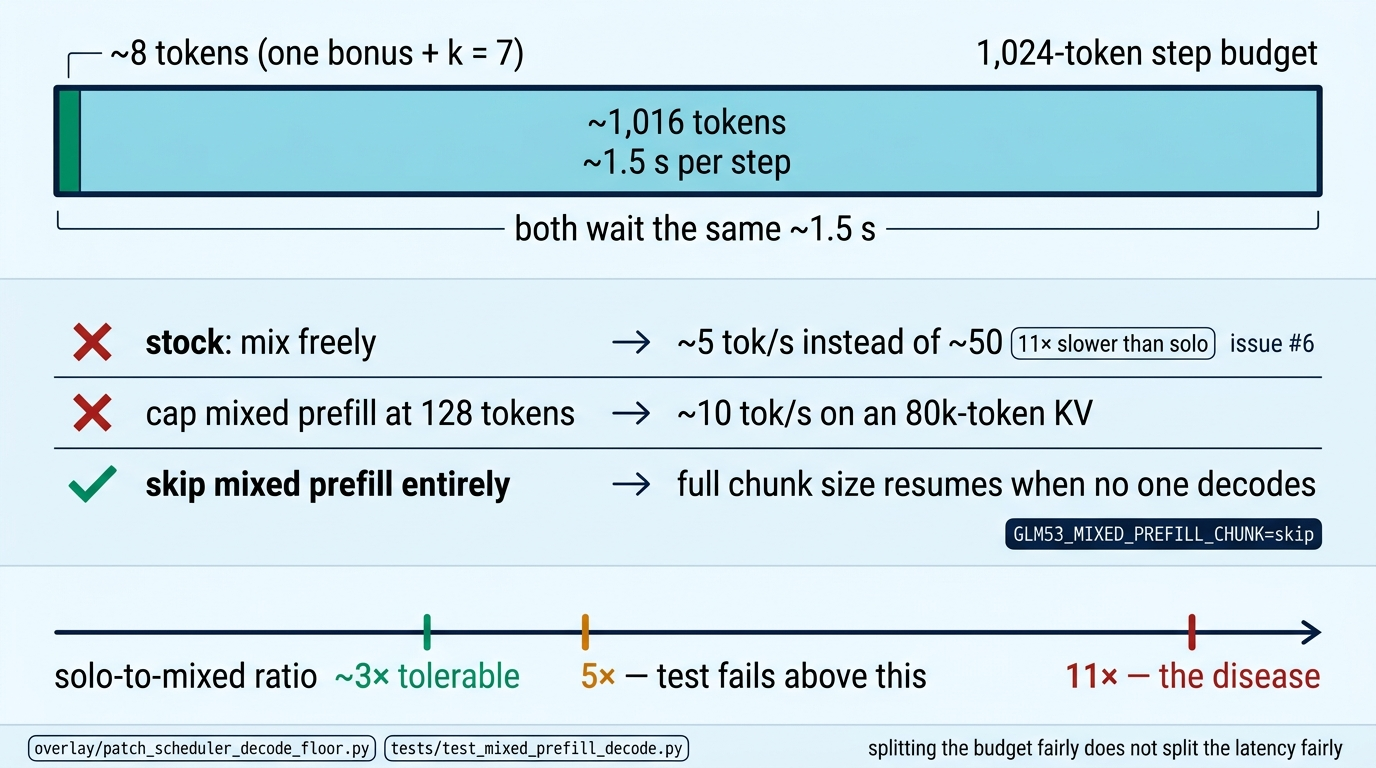
\includegraphics[width=\textwidth]{figures/ch16-mixed-decode.png}
\caption{Why a fair split of the step budget is not a fair split of latency. A
decode lane needs about 8 tokens of the 1{,}024-token engine step --- one
bonus plus the drafter's seven --- while the leftover $\sim$1{,}016 admit a
peer's sparse-MLA cold-prefill chunk costing about 1.5\,s per step, and both
lanes then wait it out: decode ran at $\sim$5 \tokspersec{} instead of
$\sim$50, roughly $11\times$ slower than solo. The instinctive remedy of
capping mixed prefill at 128 tokens was tried and was not enough --- the
sparse indexer carries a large per-step fixed cost, and mixed decode still
crawled at $\sim$10 \tokspersec{} on an 80k-token KV --- so the shipped policy
skips mixed prefill entirely while any peer is decoding, resuming full chunk
size the moment no one does. The live regression test fails above a $5\times$
solo-to-mixed ratio; $\sim$3$\times$ is tolerable overlap.}
\label{fig:proof-mixeddecode}
\end{figure}

\subsection{The one-line clamp: corruption that lands elsewhere}

The kpool tail is a one-block circular scratch cache: block size equals
\code{index_kpool} (4), and its block-table row holds a \emph{single} entry.
vLLM's generic paged slot-mapping Triton kernel computes
\code{block_indices = pos // block_size} and indexes the row with a mask that
guards only token validity --- nothing bounds the index against the row's
width. For the tail group, every token at \code{pos >= block_size} reads past
the one entry, and the kpool seed and update kernels then write through
whatever garbage block id came back. Generations of roughly 2{,}000 tokens
hit it reliably. The failure is insidious in exactly the way silent
corruption always is: a finished request is not proof the writes were
in-bounds, because most overruns land inside the shared pool and corrupt
\emph{another layer's} indexer state.

The fix in
\repofile{overlay/patch_kpool_tail_slotmap.py} is one Triton line:
\code{tl.minimum(block_indices, block_table_stride - 1)}. For the
tail's stride-1 row it restores the circular addressing the seed kernel
already documents, and it is provably an identity for every other KV group,
since no other group legitimately needs more blocks than its row holds. The
mechanism was credited to a sibling community recipe's write-up
(\repofile{docs/KPOOL_TAIL_BUG.md} in vcruz305's GLM Spark recipe). The
host test pins the arithmetic: with row \code{[17]} and block size 4,
positions 0--63 must wrap onto the same four slots, and the \emph{unclamped}
mapping must raise an index error at position 4 --- proof the patch is load-bearing, not decorative.

\begin{hbnote}
Both fixes are small because the analysis was exact; both carry tests that
reproduce the incident rather than merely asserting the patch applied.
\end{hbnote}

\FloatBarrier

Two things in this system have quietly changed category. A reservation is
no longer a number somebody once chose --- it is a claim about the largest
request the scheduler is permitted to construct, and where nobody has
re-derived that claim, the distance between it and the truth sits locked in
the process for the life of the serve. And a prompt is no longer text: on a
cache that counts only whole 3{,}584-token pages, the first twenty bytes of
a rendering decide whether the twenty thousand behind them are free or cost
26.54 seconds. Bytes are held by allocations and by strings alike, and both
classes yield to the same instrument --- a bound, plus a guard that fails
closed the moment the bound's assumptions drift.

\section*{Takeaways}

\begin{itemize}
  \item Reconcile before you reclaim, then size by legal maximum rather
    than tuned estimate: the 5036.40\,MB receipt was reproduced to the byte
    from the sizing formula before anyone patched it
    (\Cref{sec:proof-workspace}), and the shipped bound's chunk list is
    provably identical to stock over 400 random legal batches where the
    rejected REQS${=}8$ tuning would have silently split legal prefills ---
    4.75--4.85\,GiB returned to the KV pool at the shipped
    \code{MAX_NUM_SEQS=4}.
  \item A proof is only as durable as the guard around it. Guards must
    cover their worst case --- the \code{compress_ratio > 1} clause skipped
    exactly the combination that under-sizes --- and every equivalence test
    needs a power test proving it can fail, or ``nothing changed'' is
    unfalsifiable.
  \item A page-granular prefix cache makes prompt bytes an interface: one
    conditional header cost every thinking toggle a full re-prefill ---
    26.54\,s on a 21{,}642-token prompt --- until PR~63 made thinking-off a
    strict extension of thinking-on (\Cref{sec:proof-pr63}). Test the
    template shape your traffic actually has: that regression only
    manifested with tools present.
  \item Cold benchmarks must prove their own coldness: on a serve with no
    cache-reset endpoint, where recycled pages once swung cold TTFT by
    5$\times$, prompt salting plus per-request hit-counter deltas make a
    cache-hit cold rung self-incriminating.
  \item Small exact interventions beat broad tuning: a skip-mixed-prefill
    policy against the $11\times$ decode collapse and a one-line
    \code{tl.minimum} clamp against cross-layer KV corruption, each shipped
    with a test that replays the incident.
\end{itemize}

\chaptertransition{Every discipline in this chapter is the same move made
at a different scale: bound the claim, then refuse to serve where the bound
stops. The last chapter of the GLM story runs that move against the two
things a serving recipe is least able to prove --- the weights themselves,
and hardware the lab does not own --- and closes on the open repository
where community pull requests, human and AI co-authored alike, arrive
carrying their own receipts. It opens with a published refusal direction
that is mathematically immaculate and, measured against stock \code{o_proj},
indistinguishable from a random unit vector: which leaves the question of
how you edit a 320B-class model's behavior at load time once the elegant
method has failed its own measurement.}

% =============================================================================
% Chapter 17 — Transplants, Four Sparks, and the Open Lab (closes Part II
% and the book; the appendix and CTA follow)
% =============================================================================

\chapter{Transplants, Four Sparks, and the Open Lab}
\label{ch:transplants}

The published refusal-direction vectors for abliterating GLM-5.3-Flash ---
surgically removing the model's refusal behavior by editing its weights ---
are mathematically sound and, on this model, empirically useless. Measured
against stock \code{o_proj}, their maximum projection
$\lvert r^{\top}W\rvert$ was $0.084$ --- what the overlay's own tests record
as random-unit-vector level.
The publisher's own projection variants top out at 9/32 on their
refusal-bypass gate, a 32-prompt suite scoring how many refusals the edit
actually removes; byte-copying a donor's weights scores 32/32. The lab
measured that rather than assuming it, and the measurement is why the GLM
recipe's weight-editing pipeline is a byte transplant governed by a sha256
manifest rather than an elegant orthogonalization.

That pipeline is the first of this closing chapter's three subjects, and
none of them has a counterpart anywhere in Part I. \emph{Editing a
model's weights at load time} --- not patching Python, not swapping a
checkpoint, but rewriting specific tensors in memory, on both TP ranks,
between weight load and CUDA-graph capture, with the on-disk artifact
untouched --- is a capability the DeepSeek deployment never needed. The
second is the honest version of a question \Cref{ch:scaling} answered with
measurements: what does this lab publish when it wants to support hardware
it does not own? The third is the thing the whole book has been quietly
demonstrating without ever naming: the lab itself runs in public, and its
governance --- issue forms, PR templates, credit corrections, maintainership
handovers --- encodes the same evidence culture as its patches.

Each subject generalizes past this kit, and all three converge on one
answer: scope the claim to the evidence, and fail loud where the evidence
stops. Load-time weight surgery is a pattern for varying a served model
without forking its pinned artifact; the isolated, labeled TP=4 lane is a
template for shipping a configuration you cannot test; and the governance
machinery is what keeps a serving recipe trustworthy once more hands than
yours are in it. The final section then closes both Part II and the book.

\section{Editing weights at load time}

The capability this section describes was bought well before anyone knew
it would be needed, by a quiet decision at quantization time: the quant
recipe \emph{excludes} \code{self_attn.o_proj} from EXL3 quantization
(\repofile{ablit/LAYER_MAP.json} records
\code{quant_ignore_includes_o_proj: true}), so every output projection
stays native bf16. A trellis-packed tensor cannot lawfully be edited in
memory; a plain floating-point one can --- and that is the entire
precondition for everything that follows.

The GLM recipe's abliteration option (\envvar{ABLIT=1}, default off) removes
the model's refusal behavior by editing those output projections over a
configured layer range at model-load time, inside the serving container,
after \code{load_weights} and before CUDA-graph capture. Nothing on disk is
rewritten: the EXL3 checkpoint's bytes are exactly as pinned, and flipping
the feature off is a restart, not a re-download. The overlay installer
(\repofile{overlay/patch_ablit.py}) appends two hook lines to the tails of
\code{Glm5NextModel.load_weights} (layers 0--44) and
\code{Glm5NextMTP.load_weights} (layer 45), each calling
\code{maybe_apply(self)} --- inert unless \envvar{ABLIT} is exactly \code{1},
in the recipe's usual one-spelling-of-on style (\Cref{ch:patches}).

\subsection{The projection math, and why it lost}

One line of linear algebra carries this subsection, and three claims hang off
it: what the edit removes, what it leaves untouched, and why applying it to
two tensor-parallel shards independently gives the same answer as applying it
once. The third is what makes a load-time edit legal on a two-node serve at
all.

The classic abliteration method --- the one the runtime calls \code{proj} ---
orthogonalizes each weight against a published \emph{refusal direction} $r$,
a 4096-dimensional unit vector in \code{o_proj}'s output space:
%
\[
W' \;=\; \Bigl(I \;-\; \alpha\,\frac{r\,r^{\top}}{\lVert r\rVert^{2}}\Bigr)\,W,
\qquad\text{so that}\qquad
r^{\top} W' \;=\; (1-\alpha)\,r^{\top} W .
\]
%
At $\alpha=1$ the refusal component is removed exactly; at the published
$\alpha_{\mathrm{ref}}=3.0$ --- the recipe default \envvar{ABLIT_ALPHA=3.0}
--- it is inverted and doubled, a deliberate over-projection. The overlay's
test suite (\repofile{tests/test_ablit.py}) verifies this linear algebra to
unusual depth: the $(1-\alpha)$ relation holds in fp32 to a max-abs residual
of $10^{-4}$; the edit survives the bf16 serve-dtype roundtrip with error
below $0.05$; components orthogonal to $r$ are preserved against a QR-derived
63-dimensional basis; and --- the property that makes load-time application
legal at all --- editing the full $4096 \times 8192$ weight versus editing
two $4096 \times 4096$ column shards independently and concatenating agrees
to under $10^{-2}$. The edit is a row-space operation; \code{o_proj} is a
\code{RowParallelLinear} whose 4096 output rows are replicated on every
rank. Each TP rank therefore applies the identical formula to its own
input-dim shard with no collective, and the post-allreduce result is
consistent (\Cref{fig:ablit-projection}).

\begin{hbwarstory}
The projection method is mathematically sound and, on this model,
empirically useless --- and the repository measured that rather than assuming it.
The shipped refusal-direction vectors turned out to be \emph{statistically
random against stock \code{o_proj}}: the maximum $\lvert r^{\top}W\rvert$
was $0.084$, exactly random-unit-vector level. The directions have
essentially no projection onto the weights they were supposed to edit. The
publisher's own projection variants top out at 9/32 on their refusal-bypass
gate, while the donor's byte-copied weights score 32/32. The \code{proj}
path was therefore kept only for user-extracted custom directions, and
\envvar{ABLIT_METHOD=auto} routes to a different mechanism entirely: a
byte transplant.
\end{hbwarstory}

\begin{figure}[htbp]
\centering
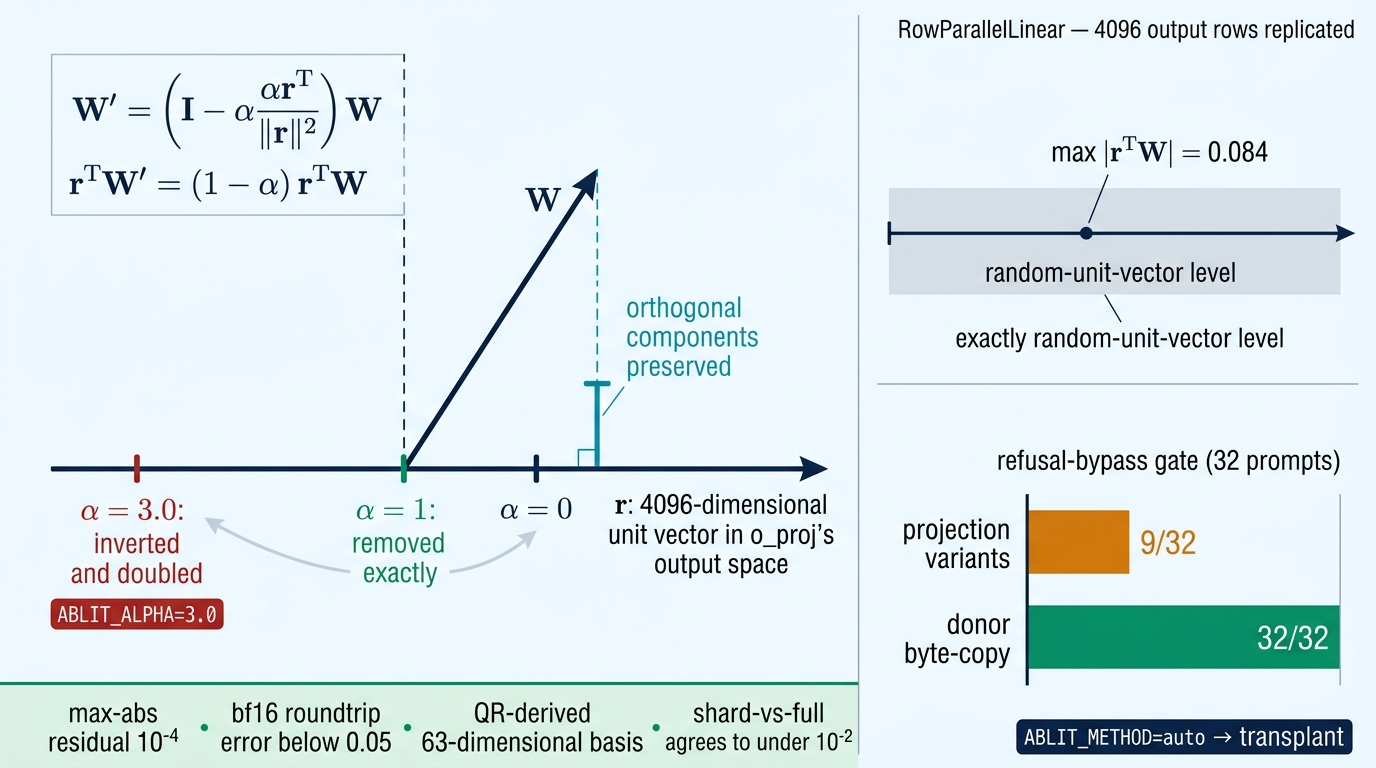
\includegraphics[width=\textwidth]{figures/ch17-projection-retired.png}
\caption{The elegant method, and the measurement that retired it. Classic
abliteration orthogonalizes each \code{o_proj} weight against a published
refusal direction $r$, so that
$r^{\top}W' = (1-\alpha)\,r^{\top}W$: at $\alpha=1$ the refusal component is
removed exactly, and at the published $\alpha=3.0$ it is inverted and doubled,
while components orthogonal to $r$ are untouched. The overlay's tests verify
all of that to unusual depth --- including that editing the full
$4096 \times 8192$ weight and editing two $4096 \times 4096$ column shards
independently agree to under $10^{-2}$, which is what makes a per-rank
load-time edit legal. What the lab then measured is the rest of the story: the
shipped directions' maximum $\lvert r^{\top}W\rvert$ against stock
\code{o_proj} was $0.084$, at random-unit-vector level. The publisher's
own projection variants top out at 9/32 on their refusal-bypass gate;
byte-copying the donor's weights scores 32/32.}
\label{fig:ablit-projection}
\end{figure}

\subsection{Byte-transplant: donor surgery with a manifest}

The mode that actually works, and the default when its tensors are present,
is \code{transplant}: byte-replace the stock \code{o_proj} weights of layers
15--45 --- 31 tensors, including the checkpoint's MTP block at layer 45 ---
with the corresponding tensors from an already-abliterated donor,
\code{dealignai/GLM-5.3-Flash-UNCENSORED-NVFP4}. This reproduces the
published \code{dealign-oproj-transplant} recipe
(\code{drowzeys/keys-GLM-5.3-Flash-NVFP4-ablit-l15-45-anchorstock}). The
trick that makes a cross-checkpoint transplant legal: this EXL3 checkpoint's
\code{o_proj} tensors are byte-identical to the NVFP4 body's --- native bf16
in both, same 120-shard layout --- so a donor tensor drops in exactly.
Layers 0--14 are deliberately left stock as \emph{safety anchors}
(\Cref{fig:transplant-map}); a stock early stack is part of the published
recipe, not an omission. Fidelity was checked against the published
fingerprint: mean relative delta $0.126$, with the layer-44 outlier measured
at $0.737$ against the published $0.74$.

Mechanically, each donor tensor arrives as a raw bf16 file
(\code{L15.bin} through \code{L45.bin}) plus a \repofile{MANIFEST.json} entry carrying shard, key, dtype,
shape, byte count, and per-tensor sha256. The runtime
(\repofile{overlay/ablit_runtime.py}) re-verifies hashes at load, checks
exact byte counts and BF16 dtype, and slices the donor's \emph{input}
dimension per TP rank --- \code{donor[:, rank*local_in:(rank+1)*local_in]}
after asserting \code{full_in == local_in * world} --- so each rank
transplants exactly its shard. The test suite proves the rank-0/rank-1
concatenation equals the donor byte-for-byte.

Two smaller checks carry real
scar tissue. A per-layer relative-$L_2$ delta must exceed $0.1$, guarding
against transplanting stock-identical tensors from a wrong donor revision.
And the donor buffer is explicitly moved to the weight's device, memorialized
in a comment --- ``proj path already does \code{r.to(weight.device)};
transplant forgot'' --- after a live-serve crash where the delta computation
mixed CPU and CUDA tensors. The DFlash2 drafter is never touched, but
\envvar{ABLIT_INCLUDE_MTP=1} transplants the MTP block's own
\code{o_proj}, because a stock MTP head keeps proposing refusals that the
edited target then rejects.

\begin{hblesson}
Every failure in the abliteration path is a hard \code{AblitError}: missing
manifest, missing tensors, missing direction file, bad layer range, shape
mismatch --- and, crucially, an enabled run that edits \emph{zero} layers
raises ``no o\_proj was edited'' rather than serving quietly. The runtime's
own phrase is the doctrine: \emph{fail loud beats silent stock weights}.
An operator who asked for an abliterated serve and got a stock one would
attribute the model's refusals to the method, publish a wrong conclusion,
and never see an error. This is \Cref{ch:patches}'s fail-closed patch
discipline applied to a new asset class: when the payload is weights, a
silent no-op is not a degraded mode --- it is a false experimental result.
\end{hblesson}

\begin{figure}[htbp]
\centering
\adjustbox{max width=\textwidth}{%
\begin{tikzpicture}
  % ---- layer strip: 0.28 cm per layer ----
  \node[hbtitle, anchor=south west] at (0,1.10)
    {o\_proj transplant map (LAYER\_MAP.json: 46 entries, hidden 4096)};
  % anchors 0-14 (15 layers)
  \draw[fill=lightgray!45, draw=hbSteel, thick] (0,0) rectangle (4.20,0.9);
  \node[font=\scriptsize, align=center] at (2.10,0.45)
    {layers 0--14\\safety-anchor (stock)};
  % edits 15-44 (30 layers)
  \draw[fill=hbAmber!30, draw=hbAmber!80!black, thick] (4.20,0) rectangle (12.60,0.9);
  \node[font=\scriptsize, align=center] at (8.40,0.45)
    {layers 15--44 --- role \emph{edit} (30 tensors, bf16 byte-copy)};
  % MTP 45
  \draw[fill=hbAccent!12, draw=hbAccent!70!black, thick] (12.60,0) rectangle (13.30,0.9);
  \node[font=\tiny, align=center] at (12.95,0.45) {45\\MTP};
  % boundary labels
  \node[hblabel, anchor=north] at (4.20,-0.05) {15};
  \node[hblabel, anchor=north] at (12.60,-0.05) {45};
  % arrow from edit region to slicing
  \draw[hbflow] (8.40,-0.15) -- (8.40,-1.02)
    node[hblabel, midway, right=1.5mm, align=left]
    {end of load\_weights,\\before CUDA-graph capture};
  % ---- per-rank slicing ----
  \node[hbtitle, anchor=south west] at (0,-1.45)
    {per-rank slice at load};
  \node[hblabel, anchor=south west] at (4.1,-1.45)
    {(input dim sharded; 4096 rows replicated)};
  \draw[fill=hbBlue!8, draw=hbSteel, thick] (0,-2.9) rectangle (4.5,-1.6);
  \node[font=\scriptsize, align=center] at (2.25,-2.25)
    {donor[:, 0:in/2]\\$\rightarrow$ rank 0};
  \draw[fill=hbBlue!8, draw=hbSteel, thick] (4.5,-2.9) rectangle (9.0,-1.6);
  \node[font=\scriptsize, align=center] at (6.75,-2.25)
    {donor[:, in/2:in]\\$\rightarrow$ rank 1};
  \draw[decorate,decoration={brace,amplitude=4pt,mirror}, thick, color=hbSteel]
    (0,-3.05) -- (9.0,-3.05)
    node[hblabel, midway, below=5pt]
    {rank 0 $\Vert$ rank 1 $=$ donor, byte-exact (tested at layers 16, 20, 31, 44)};
  \coordinate (manref) at (9.0,-2.25);
  \node[hbpatch, right=8mm of manref, align=left, font=\scriptsize] (man)
    {MANIFEST.json:\\shard, key, dtype,\\shape, nbytes, sha256\\--- re-verified at load};
  \draw[hbarrow, dashed] (man.west) -- (manref);
\end{tikzpicture}%
}
\caption{The transplant map. Layers 0--14 stay stock as safety anchors;
layers 15--45 (including the MTP block) have their bf16 \code{o_proj}
tensors byte-replaced with donor weights, sliced per TP rank along the input
dimension and verified against per-tensor sha256 manifests. The on-disk EXL3
checkpoint is never modified.}
\label{fig:transplant-map}
\end{figure}

\begin{table}[htbp]
\centering\small
\caption{The three abliteration knobs the prose discusses
(\repofile{.env.example} documents the full surface; all knobs are inert
unless \envvar{ABLIT} is exactly \code{1}).}
\label{tab:ablit-knobs}
\begin{tabular}{ll>{\raggedright\arraybackslash}p{6.4cm}}
\toprule
Knob & Default & Effect \\
\midrule
\envvar{ABLIT} & 0 & master gate; any value but \code{1} is stock \\
\envvar{ABLIT_METHOD} & auto & \code{transplant} when donor tensors are
present, else \code{proj} \\
\envvar{ABLIT_ALPHA} & 3.0 & $\alpha$ in the projection formula; 1.0 is pure
removal, 3.0 the published over-projection \\
\bottomrule
\end{tabular}
\end{table}

\section{Fetching 2.7\,GiB instead of 164\,GiB}

The donor is a full 320B-class checkpoint: roughly 164\,GiB across 120
safetensors shards. The transplant needs 31 tensors out of it.
\repofile{ablit/fetch_transplant.py} refuses to pay for the difference: it
pulls \emph{only the \code{o_proj} byte ranges} over HTTP Range requests ---
about 2.7\,GiB total --- and never materializes the donor checkpoint at all
(\Cref{fig:range-fetch}).

The flow is a small exercise in trusting the right source. The fetcher reads
\repofile{LAYER_MAP.json} and selects the layers whose role is \code{edit}
or \code{mtp-edit}; but for shard placement it fetches the donor's own
\repofile{model.safetensors.index.json} weight map. Where the two
disagree it prints a note and uses the donor index --- the map is a hint,
the donor is truth. Per layer it then reads the shard's first 8 bytes (the
safetensors header length), fetches the JSON header, looks up the tensor's
\code{data_offsets}, and issues a range request for exactly those bytes.
Transfers run in 8\,MiB chunks with 4 retries under a linear backoff of
$3\times\text{attempt}$ seconds, and resume \emph{within} a partially
fetched range. Each tensor is written via a \code{.tmp} file and atomic
rename, and \repofile{MANIFEST.json} is updated after \emph{every} tensor.
An interrupted fetch therefore loses at most one tensor's progress, and a
rerun skips any file whose sha256 already matches the manifest. The final line
reports \code{ok/31 tensors} and the gigabytes actually moved. The manifest
this produces is the same one the runtime verifies at load: the fetch tool
and the serve share one contract, keyed by hash.

Nothing in that flow is specific to abliteration. A safetensors shard carries
a JSON header naming every tensor's byte offsets, so any checkpoint served by
a host that honours Range requests is randomly addressable at tensor
granularity --- which is what turns ``31 tensors out of 120 shards'' from a
164\,GiB download into a 2.7\,GiB one.

\begin{figure}[htbp]
\centering
\adjustbox{max width=\textwidth}{%
\begin{tikzpicture}[node distance=7mm and 12mm]
  % donor shard stack
  \node[hbfaint, minimum width=32mm, align=center] (s1)
    {model-00001-of-00120\\.safetensors};
  \node[hbfaint, below=2.5mm of s1, minimum width=32mm, align=center] (s2)
    {model-00029-of-00120\\(holds an o\_proj)};
  \node[hbfaint, below=2.5mm of s2, minimum width=32mm, align=center] (s3)
    {\vdots};
  \node[hbfaint, below=2.5mm of s3, minimum width=32mm, align=center] (s4)
    {model-00120-of-00120};
  \begin{scope}[on background layer]
    \node[hbgroup, fit=(s1)(s4),
      label={[hbtitle]above:donor: 120 shards, \(\approx\)164\,GiB}] (donor) {};
  \end{scope}
  % header pipeline
  \node[hbbox, right=20mm of s2, align=left, font=\scriptsize] (hdr)
    {1. read first 8 B (header length)\\
     2. fetch JSON header\\
     3. data\_offsets[key] $\rightarrow$ [a, b)\\
     4. Range: bytes=8+n+a .. 8+n+b-1};
  \draw[hbflow] (donor.east |- hdr.west) -- (hdr.west)
    node[hblabel, midway, above=1mm] {per tensor};
  % output
  \node[hbgpu, right=26mm of hdr, align=center] (out)
    {ablit/transplant/\\L15.bin \ldots{} L45.bin\\31 tensors, \(\approx\)2.7\,GiB};
  \node[hbpatch, below=5mm of out, align=center, font=\scriptsize] (mani)
    {MANIFEST.json\\updated after every tensor\\sha256 per file};
  \draw[hbflow] (hdr) -- (out)
    node[hblabel, midway, above=1mm, align=center, font=\tiny]
    {8\,MiB chunks \(\cdot\) 4 retries\\.tmp + atomic rename};
  \draw[hbarrow, <->] (out) -- (mani)
    node[hblabel, midway, right=1mm] {resume: matching hash $\Rightarrow$ skip};
  % authority note
  \node[hblabel, below=4mm of hdr, align=center]
    {shard placement from the donor's own index.json ---\\
     LAYER\_MAP.json is a hint, the donor is truth};
\end{tikzpicture}%
}
\caption{Surgical fetching: HTTP Range requests extract the 31 \code{o_proj}
tensors (about 2.7\,GiB) from the donor's 120 shards (about 164\,GiB)
without ever downloading a shard. Every tensor is hash-manifested as it
lands, making the fetch resumable per tensor and the manifest the shared
contract between fetcher and runtime.}
\label{fig:range-fetch}
\end{figure}

\section{Honest scaling: a launcher for hardware the lab does not own}

The transplant scoped every claim to a hash it could verify; the chapter's
second subject faces the same test with no evidence to offer at all.
\Cref{ch:scaling} showed the DeepSeek recipe scaling to a third Spark with
measurements in hand. The GLM repository faces the same demand --- users with four
GB10s asked for TP=4 --- from a weaker position: the lab has no 4-Spark kit.
Its answer, merged as PR \ghissue{105} on the GLM tracker, is
\repofile{start-tp4.sh}: a roughly 90\,\% structural clone of
\repofile{start.sh} whose header says exactly what it is ---
``\textsc{experimental} \ldots{} Optional sibling of start.sh. Does not
change the supported 2$\times$ TP=2 path. \emph{Untested here (no 4-Spark
kit).} A user with four GB10s can try.'' The claim is scoped to what was
verified: the script's structure, not its behavior on real hardware.

The interesting engineering is in how the untested path is \emph{isolated}
from the tested one. The launcher sources \repofile{.env} and then layers
\repofile{.env.tp4} on top (auto-copied from \repofile{.env.tp4.example} on
first run, and git-ignored). The overlay wins over the two-node knobs, and
\repofile{start.sh} never reads the file --- so a four-node experiment
cannot leak a single variable into the supported lane. Container names are
namespaced the same way: \code{glm53-exl3-tp4-head} and \code{-w1/-w2/-w3},
``so a TP=2 serve is not accidentally reused.'' The corollary is spelled
out too: \code{./start.sh stop} does not know about ranks 2/3 --- each
topology owns its own stop path. The rest is generalization plumbing:
per-rank \envvar{WORKER2_*} / \envvar{WORKER3_*} variable families
defaulting to the rank-1 values, a rank-switch helper family behind every
SSH, cache, and NIC pin, a preflight that loops all three workers, and even
a deliberately preserved dead-code heredoc so a \code{diff} against
\repofile{start.sh} stays legible. Notably, no scheduler or KV retuning is
attempted: the same
\envvar{GPU_MEM_UTIL=0.87}, \code{MNBT} 7168, and \code{max_num_seqs} 4
ride along, because inventing tuned numbers for unmeasured hardware would
be exactly the kind of claim this repository refuses to make.

The price of that isolation is duplication: a second launcher that is roughly
90\,\% a clone of the first, kept diff-legible on purpose down to a preserved
dead-code heredoc. That is the trade being made --- redundancy in the
repository in exchange for a supported lane a four-node experiment cannot
reach (\Cref{fig:tp4-containment}).

\begin{figure}[htbp]
\centering
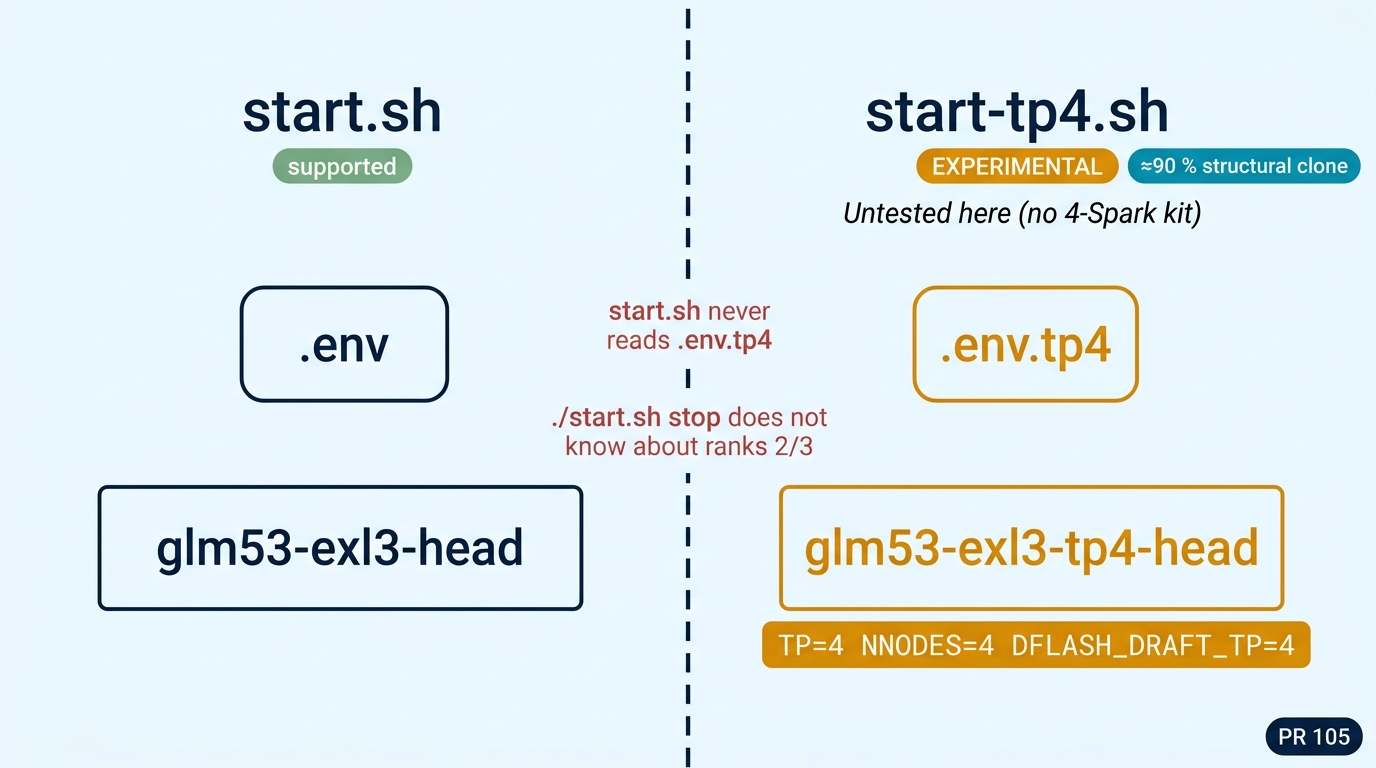
\includegraphics[width=\textwidth]{figures/ch17-tp4-containment.png}
\caption{Shipping a configuration you cannot test. \repofile{start-tp4.sh}
(PR \ghissue{105}) is roughly a 90\,\% structural clone of
\repofile{start.sh}, and the engineering is in the barrier rather than the
clone: both lanes read \repofile{.env}, but only the TP=4 launcher layers
\repofile{.env.tp4} on top --- \repofile{start.sh} never reads that file, so a
four-node experiment cannot leak a single variable into the supported lane.
Container names are namespaced the same way, and each topology owns its own
stop path, because \code{./start.sh stop} does not know about ranks 2/3. No
scheduler or KV retuning rides along: \envvar{GPU_MEM_UTIL=0.87}, MNBT 7168
and \code{max_num_seqs} 4 are unchanged, because inventing tuned numbers for
unmeasured hardware would be exactly the kind of claim this repository refuses to
make. The price is duplication, kept diff-legible on purpose down to a
preserved dead-code heredoc.}
\label{fig:tp4-containment}
\end{figure}

\begin{lstlisting}[language=bash]
# .env.tp4 -- layered over .env by start-tp4.sh ONLY (start.sh never reads it)
TP=4  NNODES=4  DFLASH_DRAFT_TP=4     # shard the drafter across all four ranks
NCCL_CROSS_NIC=1                      # ring/switch fabric, not one direct cable
WORKER2_IP=10.0.0.3  WORKER3_IP=10.0.0.4
HEAD_CX7_IB=rocep1s0f0,rocep1s0f1     # dual-port ring: both CX7 HCAs, comma list
CONTAINER_HEAD=glm53-exl3-tp4-head    # ... -w1 -w2 -w3: a TP=2 serve
                                      # can never be reused by accident
\end{lstlisting}

\begin{table}[htbp]
\centering\small
\caption{What the \repofile{.env.tp4} overlay changes relative to the
supported two-node lane.}
\label{tab:tp4-deltas}
\begin{tabular}{>{\raggedright\arraybackslash}p{3.4cm}>{\raggedright\arraybackslash}p{3.3cm}>{\raggedright\arraybackslash}p{5.6cm}}
\toprule
Knob & TP=2 (supported) & TP=4 (experimental) \\
\midrule
\envvar{TP} / \envvar{NNODES} & 2 / 2 & 4 / 4 \\
\envvar{DFLASH_DRAFT_TP} & 2 & 4 (drafter sharded across all ranks) \\
\envvar{NCCL_CROSS_NIC} & 0 (one direct QSFP cable) & 1 (ring or switch among
all ranks) \\
Worker set & \envvar{WORKER_*} only & adds \envvar{WORKER2_*} /
\envvar{WORKER3_*} (10.0.0.3 / 10.0.0.4), defaults mirroring rank 1 \\
HCA pins & one HCA per node & comma-separated dual-port lists supported;
\code{_tp4_first_ib} picks the first for GID preflight \\
Containers & \code{glm53-exl3-head} / \code{-worker} &
\code{glm53-exl3-tp4-head} / \code{-w1/-w2/-w3}; own \code{stop} and
per-rank \code{logs 1|2|3} \\
Scheduler / KV tuning & measured keeps & unchanged --- no invented numbers
for unmeasured hardware \\
\bottomrule
\end{tabular}
\end{table}

The contrast with \Cref{ch:scaling} is worth one paragraph, because the two
labs hit different walls. DeepSeek-V4-Flash's TP=3 required eleven anchored
model-code edits, a padded attention geometry, and a warring pair of pad
resolutions before a third rank could even boot --- and then shipped with a
measured ledger of what three nodes buy and cost. GLM-5.3-Flash's TP=4 is,
architecturally, ``purely more ranks'': no divisibility wall, no pad, the
same vLLM flags. What it lacks is evidence, and the repository treats missing
evidence exactly as \Cref{ch:scaling}'s repository treated numerics risk: give
the risky topology its own launcher, its own env file, its own container
namespace, and its own stop path, so the experiment cannot contaminate the
production lane. And label the untested part untested, in the header,
where a user reads it before running anything. The earlier prefill study
had already set expectations in the same spirit: TP=4 is ``not
$\sim$2$\times$, different topology, and this is a 2-node recipe.''

\begin{hbnote}
\textbf{What the next edition owes this section.} The four-Spark lane is the
one place this book documents a configuration nobody has run. When a
four-node kit exists it will get the treatment \Cref{ch:scaling} gave the
third Spark --- one knob per boot, a dated ledger, a fabric census, and a
verdict that may well be negative. The question is already sharp. Adding a
third node cut the bytes each rank must stream to $\approx$11.5\,GB and the
streaming model priced the step at $\approx$48\,ms; measured decode came
out at 64.3 \tokspersec{}, no faster than two nodes, because fixed per-step
cost ate the entire bandwidth gain (\Cref{ch:perf}). A fourth node inherits
that arithmetic and adds collectives on top of it. Whether the curve bends
or flattens again is not derivable from the byte model. It has to be
measured --- and until it is, this section is the honest end of the story.
\end{hbnote}

\section{The fabric truths a fourth Spark rests on}

Whether at two nodes or four, every rank of this deployment stands on a
stack of RoCEv2 facts that were learned the hard way and then promoted into
preflight code. \Cref{ch:fabric} covered the DeepSeek pair's fabric; the GLM
repository's contribution is the \emph{GID index} lore, and it generalizes to any
multi-NIC RDMA cluster.

A RoCE GID table maps small integer indices to addresses, per NIC, per
node --- and nothing guarantees two nodes agree. On the second GLM kit
(GLM tracker \ghissue{26}, contributed by im0xMagnus), the RoCE-v2
\code{::ffff:<ip>} entry sat at index 4 on the head and index 3 on the
worker; the only index the two nodes had in common (2) was a RoCE-v1 entry,
which cannot serve a fabric pinned to \envvar{NCCL_IB_ROCE_VERSION_NUM=2}.
No single shared \envvar{NCCL_IB_GID_INDEX} could ever work on that pair
--- the knob's very shape was wrong. The fix is per-rank GID pins
(\envvar{HEAD_GID} / \envvar{WORKER_GID}, defaulting to the shared index 3),
extended to \envvar{WORKER2_GID} / \envvar{WORKER3_GID} in the TP=4 overlay
(\Cref{fig:gid-mismatch}).

\begin{hbwarstory}
The nastier failure mode arrived first, as GLM tracker \ghissue{16}
(Jim Bisesi, from an independent second-kit reproduction): an
\emph{all-zero} GID entry. An empty entry passes every earlier network
check --- links up, pings fine, NCCL initializes --- and then kills its
rank roughly 60 seconds into the boot with \code{ibv_modify_qp} errno 61,
``No data available,'' deep in queue-pair state transition. By that point
any operator has long stopped watching for network errors. The launcher's
preflight now validates that each rank's GID index names a \emph{populated}
entry in that rank's own
\repofile{/sys/class/infiniband/<dev>/ports/1/gids/<idx>}. On refusal it
dumps both nodes' full 0--7 GID tables with their RoCE v1/v2 types and the
selection rule: pick each node's \code{::ffff:<ip>} entry whose type is
RoCE v2; the two indices need not match.
\end{hbwarstory}

The same promotion-to-preflight pattern covers the sub-gigabyte memory
margin: \envvar{GPU_MEM_UTIL=0.87} requires at least 105.9\,GiB free, and
nodes with resident desktop services miss that bar by under a gigabyte. The
README encodes the documented fallback pair rather than leaving the
operator to rediscover the margin from an OOM at minute forty of a weight
load. The
through-line of all three: a fact that once cost a debugging session ---
a v2 entry at different indices, an all-zero GID, a sub-gigabyte memory
margin --- is worth a preflight check that costs milliseconds, dumps its
evidence when it refuses, and turns a mid-boot rank death into a launcher
error with a remedy attached.

\begin{figure}[htbp]
\centering
\adjustbox{max width=\textwidth}{%
\begin{tikzpicture}[node distance=8mm and 16mm]
  % head GID table
  \node[hbhost, minimum width=46mm, align=left, font=\scriptsize] (head)
    {\textbf{head} --- rocep1s0f1, GID table\\[1mm]
     idx 2: fe80::\ldots{} \hfill RoCE v1\\
     idx 3: 0000:0000:\ldots:0000 \hfill \textcolor{hbAccent}{all-zero}\\
     idx 4: ::ffff:$\langle$head-ip$\rangle$ \hfill \textbf{RoCE v2}};
  % worker GID table
  \node[hbhost, right=24mm of head, minimum width=46mm, align=left, font=\scriptsize] (wrk)
    {\textbf{worker} --- rocep1s0f0, GID table\\[1mm]
     idx 2: fe80::\ldots{} \hfill RoCE v1\\
     idx 3: ::ffff:$\langle$worker-ip$\rangle$ \hfill \textbf{RoCE v2}\\
     idx 4: (empty)};
  % shared-index attempt (fails)
  \node[hbwarn, below=11mm of $(head.south)!0.5!(wrk.south)$,
        align=center, font=\scriptsize] (shared)
    {one shared NCCL\_IB\_GID\_INDEX?\\only common index (2) is RoCE v1\\
     $\Rightarrow$ cannot serve a v2 fabric};
  \draw[hbfail] (head.south) -- (shared.north west);
  \draw[hbfail] (wrk.south) -- (shared.north east);
  % per-rank pins (works)
  \node[hbgpu, below=8mm of shared, align=center, font=\scriptsize] (pins)
    {per-rank pins: HEAD\_GID=4, WORKER\_GID=3\\
     (TP=4 adds WORKER2\_GID / WORKER3\_GID)};
  \draw[hbok] (shared) -- (pins)
    node[hblabel, midway, right=1mm] {\ghissue{26}};
  % preflight annotation
  \node[hbpatch, right=10mm of pins, align=left, font=\scriptsize] (pf)
    {preflight (\ghissue{16}): index must name a\\
     populated entry on that rank's OWN NIC;\\
     refusal dumps both GID tables 0--7.\\
     All-zero entry: passes every check,\\
     kills the rank \(\approx\)60\,s in ---\\
     ibv\_modify\_qp errno 61};
  \draw[hbarrow, dashed] (pf.west) -- (pins.east);
\end{tikzpicture}%
}
\caption{Why the GID index is per-NIC state, not cluster configuration. On
the second GLM kit the RoCE-v2 entry sat at index 4 on the head and 3 on
the worker, the only common index was v1, and an all-zero entry passed
every network check before killing its rank a minute into boot. The
launcher validates each rank against its own device and prints the
evidence when it refuses.}
\label{fig:gid-mismatch}
\end{figure}

\section{The open lab}

Preflight checks are how the lab encodes its lessons for machines; its last
subject is how it encodes them for people. Everything in Part II so far --- the quantized bet, the drafter, the
proof-carrying patches, the transplants --- was built in ten days, in
public, by more than a dozen people. The repository's history (125 commits,
2026-08-26 through 2026-09-05) reads less like a solo project than like a
functioning lab with a door open: twelve named community contributors
landed substantive changes, and they cluster into three kinds of work.
Bring-up and hardening: Chris Scott's seed SM120 overlay (the repository's
literal first commit), Raymond Lucke's day-two template fix, Jim Bisesi's
GID preflight, Daniel Banu's env-only API auth, hecisaza's numeric-knob
validation, and Tutanka01's bring-up robustness work. Measurement, client,
and template infrastructure: Tutanka01's prefix-cache bench, Jenpo's
bounded Pi client configs, sovereignbrah's reasoning-effort prefix-cache
fix, and knapcio's XGrammar backports. Kernels and rightsizing:
plotarmordev's E2 kernel diagnostics and spinwait sweep, nood-co1's
indexer-workspace rightsizing, and im0xMagnus's \envvar{CG_ESTIMATE}
opt-out and per-rank-GID work.

The indexer-workspace rightsizing alone came to 1{,}743
lines --- of which 819 were tests. By September 1 the maintainership itself had
broadened: community PRs were being merged by netrunner (plotarmordev), and
a GitHub Sponsors funding model sat alongside the code. AI co-authorship is
carried openly rather than laundered: Cursor trailers on nearly all
maintainer commits, Claude Opus 5 on three community PRs, Claude Fable 5 on
two more, and two commits linking their full \code{Claude-Session} URLs.
The provenance of machine assistance is treated like any other provenance,
recorded where posterity can audit it.

What makes this durable is that the evidence culture is \emph{encoded in
the contribution machinery}, not left to the maintainer's taste. The issue
forms (PR \ghissue{126} on the GLM tracker, ported from the lab's Qwen3.8
kit) disable blank issues, enumerate the kit's actual knob surface in the
bug form's environment section, and pre-list the four most common
self-serve culprits --- incomplete weights, a slow-decode checklist keyed
to boot-log facts, the do-not-reduce-\envvar{MAX_MODEL_LEN} trap, and the
vision-request shape --- so a report arrives triaged. The improvement form
asks for measured before/after numbers.

The PR template goes further: a
contributor must say which knob, default, overlay, or kernel path changes
and the expected direction of any measured number; explain why the change
is safe on \emph{both} nodes of the two-node TP=2 lane; and show testing
that means something. In practice that is \code{bash -n} for scripts, an actual
cluster boot with boot-log facts, measured numbers in the README's own
format (median-of-5 \repofile{tests/bench_decode.py}, the cold-prefill
table), and, for any change touching the drafter, ``an acceptance
measurement, not just tok/s.'' That last clause is a whole chapter of speculative-decoding
doctrine compressed into a form field: throughput without acceptance is
exactly the number that lies (\Cref{ch:measurement}).

\begin{hbnote}
The governance even retracts. PR \ghissue{55} on the GLM tracker --- filed,
fittingly, via a Pi agent running against this very serve --- corrected the
credits. An incorrect abliteration-donor line and a contributor credit
added hours earlier the same day were dropped as ``not accurate,'' while the
genuine drowzeys recipe attribution stayed. Attribution held to the same
standard as benchmarks --- dated, checked, and publicly corrected when
wrong --- is the social mirror of Part I's measurement retractions
(\Cref{ch:lessons}): the lab versions its beliefs about \emph{people} the
way it versions its beliefs about numbers.
\end{hbnote}

\FloatBarrier

The three subjects of this chapter look unrelated until you notice they
fail in the same place. A served checkpoint is not a fixed artifact --- it
is bytes in memory that a load-time hook may lawfully rewrite, provided a
hash says which bytes and a hard error fires when none were touched. A
topology the lab cannot boot is not unsupported --- it is a claim with no
evidence behind it, shippable only inside its own launcher, its own env
file, and its own label. And a repository with a dozen hands in it is not a
governance problem but an evidence problem, solved with issue forms and PR
fields rather than with a maintainer's taste. In all three the discipline
is identical: scope the claim to what was verified, and make the boundary
where verification stops loud enough that nobody walks past it.

\section*{Takeaways}

\begin{itemize}
\item Excluding \code{o_proj} from quantization bought a capability months
early --- bf16 weights can be edited at load time, per TP rank, with the
pinned checkpoint untouched --- and measuring the method before shipping it
is what decided which edit. The published refusal directions proved
statistically random against stock \code{o_proj}, a maximum
$\lvert r^{\top}W\rvert$ of $0.084$ and 9/32 on the refusal-bypass gate, so
the recipe byte-transplants donor weights instead, at 32/32.
\item When the payload is weights, a silent no-op is a false experimental
result: every abliteration failure is a hard \code{AblitError}, and an
enabled run that edits zero layers raises. The integrity contract is a
sha256 manifest shared by fetcher and runtime --- which is also what turns
31 tensors out of 120 shards into a 2.7\,GiB HTTP Range fetch, resumable
per tensor, rather than a 164\,GiB download.
\item Honest scaling for hardware you lack means isolation plus a label:
an untested lane with its own launcher, env file, containers, and stop
path --- and no invented numbers.
\item Fabric identity is per-NIC state: GID indices need not match across
nodes, and the cure is per-rank pins plus a preflight that dumps its
evidence on refusal.
\item Governance can encode epistemics: triaged issue forms, a PR template
demanding acceptance measurements, open AI co-authorship, and credits
corrected in public.
\end{itemize}

\section{Two recipes, one method}

Set the two halves of this book side by side and almost every technical
decision diverges. Part I serves DeepSeek-V4-Flash from the vendor's own
native low-precision checkpoint; Part II bets on a community EXL3/TR3
4-bpw quant, mirrored for durability and defended by an independent KLD
panel. Part I's drafter is DSpark; Part II's is DFlash2, with its
candidate-selector lattice walk. Part I tunes and patches stock kernels;
Part II, when the fat-expert tax would not yield to configuration, wrote
its own CUDA and compiled it into the extension. One recipe reached a
third node with padded attention geometry and a measured ledger; the other
shipped a fourth-node launcher labeled untested. Even the failure modes
differ --- a starved scheduler knob here, a one-block circular slot map
there.

And yet an engineer who has read both halves will recognize that they are
the same book. Both recipes pin every artifact --- image digests, model
revisions, extension commits, patch anchors --- and refuse to run when the
bytes drift. Both apply every change fail-closed, so a fix that cannot
prove its target aborts the boot instead of serving a lie. Both measure
before believing: one knob per boot, dated receipts, noise bands,
acceptance alongside throughput, benchmarks that distrust themselves. And
both revert in public --- a withdrawn safety claim, a struck evidence
matrix, two prefill optimizations published as losses, a credit line
corrected by an agent using the very server it corrected. The bets were
opposite; the method was identical; and the method, not either bet, is
what produced two working frontier serving systems.

That is the thing to carry out of this book. The hardware on these desks
is unremarkable by datacenter standards --- two small machines and a
cable, twice over. What made a million tokens of context, speculative
decoding, vision, and tools run interactively on them was not a secret
kernel or a heroic all-nighter but a discipline applied without exception:
pin it, prove it, measure it, and say so out loud when you were wrong.
That discipline is not proprietary. It fits in a preflight check, a PR
template, a manifest, an issue form; it survives handover to new
maintainers and collaboration with machines; it worked twice, on opposite
bets, in the same small lab. Wherever your own frontier is --- whatever
model, whatever engine, whatever pair of machines --- it will work a third
time.


\backmatter
\chapter{Quick Reference}
\label{ch:appendix}
\markboth{Quick Reference}{Quick Reference}
% Backmatter chapter is unnumbered; number its tables as A.n, not 17.n.
\renewcommand{\thetable}{A.\arabic{table}}
\setcounter{table}{0}

\section*{Glossary}\addcontentsline{toc}{section}{Glossary}

Terms marked (II) belong to the GLM recipe of Part~II; the rest are
Part~I's, and several are shared.

\begin{description}
  \item[Abliteration (II)] Editing a model's weights to remove its
    refusal behavior. The GLM recipe implements it as a byte transplant
    governed by a sha256 manifest rather than as an orthogonalization,
    because the published refusal directions measured at random-unit-vector
    level against stock \code{o_proj} (\Cref{ch:transplants}).
  \item[Anemll image] The prebuilt, digest-pinned GB10 vLLM runtime
    (\repofile{ghcr.io/anemll/dspark-vllm-gx10:0.1.1}) that this recipe
    patches at boot rather than rebuilding.
  \item[B12X] The image's MoE kernel backend for GB10
    (\code{--moe-backend flashinfer_b12x}), built on CuTeDSL; runs the
    experts as W4A16 on this checkpoint.
  \item[DFlash2 (II)] The GLM recipe's drafter: a \emph{separate}
    $\approx$2.3\,GiB Qwen3-architecture draft model
    (\code{incoai/GLM-5.3-Flash-DFlash2}), run at $k{=}7$ with a trained
    block of 8 --- the structural opposite of DSpark's checkpoint-native
    design (\Cref{ch:dflash2}).
  \item[DSML] DeepSeek's markup language for tool calls
    (\code{<|DSML|tool_calls>} / \code{invoke} / \code{parameter} blocks)
    emitted as ordinary tokens and parsed server-side into structured
    \code{tool_calls}.
  \item[DSpark] The checkpoint's built-in speculative-decoding drafter:
    block drafting (block size 5) via stacked MTP stages in one non-causal
    pass, sampled left-to-right with a rank-256 Markov head.
  \item[E2 fat-expert kernels (II)] The hand-written CUDA kernels
    merged as PR~77, which removed the ``fat tax'' on fully uncached prefill
    that the profile-first campaign of \Cref{ch:quantized-bet} had priced.
  \item[EXL3 / TR3 (II)] The community quantization the GLM recipe
    serves: brandonmusic's 4-bits-per-weight trellis format
    (\code{GLM-5.3-Flash-tr3-4bpw}), chosen instead of a native NVFP4
    checkpoint --- Part~II's central bet (\Cref{ch:quantized-bet}).
  \item[GB10 / SM121] The Grace--Blackwell superchip in a DGX Spark and its
    CUDA compute capability (kernels target \code{sm_121a}); 128\,GB unified
    LPDDR5X shared by CPU and GPU.
  \item[GID (RoCE)] The per-port address table entry NCCL must select to
    speak RoCEv2 over IPv4; indexes differ per HCA and drift, hence the
    validate-and-leave-unset doctrine of \Cref{ch:fabric}.
  \item[Indexer workspace right-sizing (II)] Measuring the sparse
    indexer's scratch allocation and reserving exactly what the shapes
    require, rather than over-reserving against a guess. Merged as PR~86;
    the change came to 1{,}743 lines, 819 of them tests
    (\Cref{ch:bytes-by-proof}).
  \item[KpoolTailManager (II)] The sparse-MLA hybrid pool manager.
    It disables fine-grained prefix-cache hits, so only block-aligned tokens
    count and the alignment is the 3{,}584-token hybrid MLA page
    (\Cref{ch:bytes-by-proof}).
  \item[Lightning indexer] The model's sparse-attention scorer: 64 index
    heads, replicated on every TP rank, selecting top-$k$ compressed keys
    per query; dominates long-context prefill cost.
  \item[MLA] Multi-head latent attention: attention over a compressed latent
    KV, which every TP rank holds in full --- the reason a third GPU does not
    shrink attention work.
  \item[MTP] Multi-token prediction --- the extra model stages the drafter
    is built from; \envvar{MTP_NUM_TOKENS} is the draft depth $k$.
  \item[NVFP4 / \code{nvfp4_ds_mla}] The KV-cache dtype string of the
    default profile. On this image its 584-byte row is byte-identical to
    \code{fp8_ds_mla}; a true 4-bit row is a design, not a shipped feature
    (\Cref{ch:scaling}).
  \item[Prefix caching] Reuse of previously computed KV blocks when a new
    request shares a prompt prefix; interacts with sliding-window groups
    (\ghissue{26}) and with honest benchmarking (\Cref{ch:measurement}).
  \item[RoCE v2] RDMA over Converged Ethernet; the transport NCCL uses
    across the pair's direct 200\,Gb link.
  \item[Stage-C] The historical locally built runtime overlay
    (\repofile{vllm-dspark-runtime:dspark-nvfp4-stage-c}) whose
    \envvar{VLLM_DSPARK_*} kill-switches are no-ops on the Anemll image.
  \item[SWA] Sliding-window attention groups in the hybrid KV layout (used
    by the drafter and indexer caches), with different eviction behavior
    than the main MLA group.
  \item[TP] Tensor parallelism --- each layer's weights split across ranks,
    synchronized by collectives every step. TP=2 default; TP=3 optional in
    Part~I, and an experimental TP=4 lane in Part~II
    (\Cref{ch:transplants}).
\end{description}

\section*{Issue index}\addcontentsline{toc}{section}{Issue index}

The numbered incidents that structure this book, with the chapter that treats
each in depth. The two parts cite two different trackers, and the numbering
collides: \ghissue{26}, \ghissue{55}, and \ghissue{105} name one thing in the
DeepSeek tracker and something else entirely in the GLM tracker. The tables
are therefore kept separate, and Part~II's prose names its tracker at every
citation.

\begin{table}[htbp]
\centering\small
\caption{Part~I: DeepSeek tracker, issue-to-chapter index.}
\label{tab:appendix:issues}
\begin{tabular}{@{}ll>{\raggedright\arraybackslash}p{72mm}@{}}
\toprule
\textbf{Issue} & \textbf{Chapter} & \textbf{One-line summary} \\
\midrule
\ghissue{21} & \Cref{ch:bugs} & Encoder double-wrapped dict tool arguments \\
\ghissue{22} & \Cref{ch:bugs} & \code{nvfp4_ds_mla} dispatched to slow kernel (1 vs 17\,\tokspersec{}) \\
\ghissue{26}/\ghissue{36} & \Cref{ch:bugs} & Hybrid SWA prefix-cache collapse, then v1 overcorrection \\
\ghissue{27}/\ghissue{154}/\ghissue{211} & \Cref{ch:bugs} & Partial-prefill admission cap saga; default 1$\to$2$\to$1 \\
\ghissue{31}/\ghissue{66} & \Cref{ch:profile} & GPU \code{thinking_token_budget}; made opt-in \\
\ghissue{38}/\ghissue{72} & \Cref{ch:operations} & Restart policy vs launcher; exit-3 contract \\
\ghissue{43} & \Cref{ch:bugs} & Decode service floor during mixed prefill steps \\
\ghissue{52}/\ghissue{120} & \Cref{ch:bugs} & Assistant-final dead-state rendering; reminder tail \\
\ghissue{55} & \Cref{ch:bugs} & Truncated tool calls reported \code{tool_calls} \\
\ghissue{79} & \Cref{ch:bugs} & SHM spin-wait burning P-cores (1\,s $\to$ 2\,ms) \\
\ghissue{105} & \Cref{ch:operations} & Malformed inflight-prefill env crashed admission \\
\ghissue{117} & \Cref{ch:bugs} & JIT-cache loss $\to$ mid-serve compile $\to$ TP watchdog kill \\
\ghissue{133} & \Cref{ch:bugs} & Triton compile-key explosion on sliced pointers \\
\ghissue{136}/\ghissue{210} & \Cref{ch:bugs} & XGrammar tokens-after-termination chain \\
\ghissue{138} & \Cref{ch:patches} & Responses history replay compatibility (opt-in) \\
\ghissue{141}/\ghissue{143} & \Cref{ch:bugs} & Stochastic sparse-MLA stall; retracted safety matrix \\
\ghissue{165}--\ghissue{181} & \Cref{ch:bugs} & The image-tag false-positive 400 saga (four rounds) \\
\ghissue{172}/\ghissue{175} & \Cref{ch:bugs} & Vision pad hashing; image tokens on text router \\
\ghissue{185} & \Cref{ch:operations} & Healthcheck probed loopback on LAN-IP binds \\
\ghissue{191} & \Cref{ch:bugs} & Named-tool contract leak; thinking-off fallback \\
\bottomrule
\end{tabular}
\end{table}

\begin{table}[htbp]
\centering\small
\caption{Part~II: GLM tracker, issue and pull-request index.}
\label{tab:appendix:glm-issues}
\begin{tabular}{@{}ll>{\raggedright\arraybackslash}p{72mm}@{}}
\toprule
\textbf{Issue / PR} & \textbf{Chapter} & \textbf{One-line summary} \\
\midrule
\ghissue{6} & \Cref{ch:bytes-by-proof} & Mixed prefill/decode scheduler floor; never mix a peer prefill into a decode step \\
PR~8 & \Cref{ch:bytes-by-proof} & Compress-ratio cross-check draft, rejected by review as a blocker \\
PR~16 & \Cref{ch:transplants} & GID preflight on both nodes: an index must name a real RoCE-v2 entry \\
PR~25 & \Cref{ch:bytes-by-proof} & \envvar{CG_ESTIMATE=0}: vLLM's CUDA-graph reservation vs the 2.43\,GiB measurement \\
PR~26 & \Cref{ch:transplants} & Per-rank RoCEv2 GID (\envvar{HEAD_GID} / \envvar{WORKER_GID}); indexes differ per node \\
PR~38 & \Cref{ch:bytes-by-proof} & Numeric knob validation; the scar on the fail-closed rule \\
PR~48/PR~49 & \Cref{ch:dflash2} & \envvar{DFLASH_DRAFT_TP=2} default: sharding the drafter was a keep, not a wash \\
PR~55 & \Cref{ch:transplants} & Credits retraction: an incorrect attribution withdrawn in-tree \\
PR~63 & \Cref{ch:bytes-by-proof} & Thinking-off header divergence at token~2; a one-line guard, a full re-prefill \\
PR~77 & \Cref{ch:quantized-bet} & The E2 fat-expert CUDA kernels; the fat tax removed properly \\
PR~86 & \Cref{ch:bytes-by-proof} & Indexer workspace right-sizing (1{,}743 lines, 819 of them tests) \\
PR~105 & \Cref{ch:transplants} & Experimental \repofile{start-tp4.sh}: TP=4 shipped without the hardware to measure it \\
PR~126 & \Cref{ch:transplants} & Issue forms and PR template; the knob surface enumerated, blank issues disabled \\
\bottomrule
\end{tabular}
\end{table}

\Needspace{10\baselineskip}
\section*{Operational quick card}\addcontentsline{toc}{section}{Operational quick card}

\textbf{Part~I --- the DeepSeek recipe.}

\begin{lstlisting}[language=bash]
# Weights (head; both nodes unless NFS mode)
./prepare-dspark-model-cache.sh --official

# Start (worker first, automatically), verify, use
./start-deepseek-v4-flash-dspark.sh        # exit 3 = already up (OK)
curl -fsS http://127.0.0.1:8888/v1/models
./smoke-deepseek-v4-flash-dspark.sh
./status-deepseek-v4-flash-dspark.sh

# Full quality audit against the live pair
bash scripts/run-audit.sh --base-url http://127.0.0.1:8888/v1 \
     --model deepseek-v4-flash-vision-exp

# Any flag flip: recreate BOTH ranks (restart is not rollback)
./stop-deepseek-v4-flash-dspark.sh && ./start-deepseek-v4-flash-dspark.sh
\end{lstlisting}

Golden rules, in one place: never set \envvar{DSPARK_MODEL} or
\envvar{GPU_MEMORY_UTILIZATION} by hand; leave
\envvar{VLLM_USE_BREAKABLE_CUDAGRAPH=0}; disable \code{earlyoom} on both
hosts; treat a missing \code{finish_reason} as the first sign of silent
truncation; and archive both ranks' flight-recorder dumps together before
restarting a wedged pair.

\Needspace{10\baselineskip}
\textbf{Part~II --- the GLM recipe.} One launcher does everything; there is
no separate stop, status, or smoke script.

\begin{lstlisting}[language=bash]
# Weights (head HF cache only; start.sh does this too if missing)
./download.sh

# Start: pull public GHCR :exl3, download if missing, rsync, launch TP=2
./start.sh                    # first run copies .env.example -> .env

# Inspect and stop
./start.sh status
./start.sh logs               # head; `logs worker` for the other rank
./start.sh stop               # or ./stop.sh

# Skip stages when the weights and image are already local
SKIP_PULL=1 SKIP_DOWNLOAD=1 SKIP_SYNC=1 ./start.sh restart

# Experimental 4-Spark lane (unmeasured: the lab has no 4-Spark kit)
./start-tp4.sh                # stop | logs 1|2|3 for a worker rank
\end{lstlisting}

Golden rules for this recipe: do not pull the \code{glm53-flash-sm121:v8}
image --- it is the older NVFP4/Ray kernel, not the EXL3 build; leave
\envvar{DFLASH_DRAFT_TP} at 2, because sharding the drafter was measured a
keep rather than a wash; and read TP=4 as a shipped configuration with no
evidence behind it, which is exactly how its own authors scope it.

\section*{Sources}\addcontentsline{toc}{section}{Sources}

This handbook was written against two repositories, one per part.

\textbf{Part~I} draws on
\repofile{MiaAI-Lab/DeepSeek-v4-Flash-DSpark-2x-DGX-Spark} at commit
\code{f5665e8} (2026-09-05), reading: \repofile{README.md},
\repofile{CHANGELOG.md}, \repofile{AUDIT.md}, all of \repofile{docs/}
(including the \repofile{docs/CLAUDE/} engineering reports and A/B records),
all 42 files under \repofile{patches/}, all 66 files under
\repofile{scripts/}, \repofile{tests/}, \repofile{recipe/},
\repofile{vllm_patch_gb10/}, \repofile{lmcache/}, \repofile{files/},
\repofile{results/}, the launcher and Compose files, and
\repofile{.env.dspark.example}.

\textbf{Part~II} draws on
\repofile{MiaAI-Lab/GLM-5.3-Flash-EXL3-2x-DGX-Sparks} at commit
\code{3021f24} (2026-09-05), reading: \repofile{README.md}, all of
\repofile{docs/} (including the design notes behind indexer-workspace
right-sizing), all 21 sources under \repofile{overlay/} including the
hand-written CUDA kernels, all 19 files under \repofile{tests/}, the
\repofile{ablit/} abliteration pipeline, \repofile{examples/},
\repofile{files/}, \repofile{scripts/}, the \repofile{Dockerfile}, both
launchers (\repofile{start.sh} and \repofile{start-tp4.sh}),
\repofile{download.sh}, the example environment files, and all 125 commits
of the project's history.

Measured numbers retain their in-repository dates and lanes; readers should
treat each repository itself as the living source of truth beyond the commit
quoted here.


\brandcta[figures/linkedin-qr.png]

\end{document}
